\documentclass[12pt,UTF8,fleqn]{ctexart}
\usepackage{docmute}
\usepackage{ctex,amsmath,amssymb,geometry,fancyhdr,bm,amsfonts,mathtools,extarrows,graphicx,url,enumerate,xcolor,float,multicol,wasysym}
\usepackage{subfigure}
\allowdisplaybreaks[4]
% 加入中文支持
\newcommand\Set[2]{\left\{#1\ \middle\vert\ #2 \right\}}
\newcommand\Lim[0]{\lim\limits_{n\rightarrow\infty}}
\newcommand\LIM[2]{\lim\limits_{#1\rightarrow#2}}
\newcommand\Ser[1]{\sum_{n=#1}^\infty}
\newcommand{\SER}[2]{\sum_{#1=#2}^\infty}
\newcommand{\Int}[4]{\varint\nolimits_{#1}^{#2}#3\mathrm d#4}
\newcommand{\aIInt}[1]{\iint\limits_{#1}}
\newcommand{\IInt}[3]{\iint\limits_{#1}#2\mathrm d#3}
\newcommand{\varIInt}[4]{\iint\limits_{#1}#2\mathrm d#3\mathrm d#4}
\newcommand{\IIInt}[3]{\iiint\limits_{#1}#2\mathrm d#3}
\newcommand{\varIIInt}[5]{\iiint\limits_{#1}#2\mathrm d#3\mathrm d#4\mathrm d#5}
\newcommand{\LInt}[3]{\varint\nolimits_{#1}#2\mathrm d#3}
\newcommand{\LOInt}[3]{\varoint\nolimits_{#1}#2\mathrm d#3}
\newcommand{\LLInt}[4]{\varint\nolimits_{#1}\nolimits^{#2}#3\mathrm d#4}
\newcommand{\BLInt}[2]{\varint\nolimits_{#1}#2}
\newcommand{\varBLInt}[3]{\varint\nolimits_{#1}\nolimits^{#2}#3}
\newcommand{\BLOInt}[2]{\varoint\nolimits_{#1}#2}
\newcommand{\SIInt}[3]{\iint\limits_{#1}#2\mathrm d#3}
\newcommand{\md}[1]{\mathrm d#1}
\newcommand{\BSIInt}[2]{\iint\limits_{#1}#2}
\newcommand{\pp}[2]{\frac{\partial #1}{\partial #2}}
\newcommand{\ppx}[1]{\frac{\partial #1}{\partial x}}
\newcommand{\ppy}[1]{\frac{\partial #1}{\partial y}}
\newcommand{\ppz}[1]{\frac{\partial #1}{\partial z}}
\newcommand{\varppx}[1]{\frac{\partial}{\partial x} #1}
\newcommand{\varppy}[1]{\frac{\partial}{\partial y} #1}
\newcommand{\varppz}[1]{\frac{\partial}{\partial z} #1}
\newcommand{\BSOIInt}[2]{\oiint\limits_{#1}#2}
\newcommand{\me}[0]{\mathrm e}
\newcommand{\m}[0]{\mathrm }
\newcommand{\dd}[2]{\frac{\mathrm d #1}{\mathrm d #2}}
\geometry{a4paper,scale=0.80}
%\pagestyle{fancy}
%\rhead{习题12.1\&12.2\&12.3}
%\lhead{基础习题课讲义}
%\chead{微积分B(2)}

\pagestyle{fancy}             % 选用 fancy style
% 其余同 plain style
\fancyhf{}                    
\fancyhead[L]{基础习题课讲义}
\fancyhead[C]{\leftmark}
\fancyhead[R]{微积分B(2)}
\fancyfoot[C]{~\thepage~}
\renewcommand{\headrulewidth}{0.7pt}
\renewcommand{\footrulewidth}{0pt}
\begin{document}
\documentclass[12pt,UTF8,fleqn]{ctexart}
\usepackage{ctex,amsmath,amssymb,geometry,fancyhdr,bm,amsfonts,mathtools,extarrows,graphicx,url,enumerate,xcolor,float,multicol,wasysym}
\usepackage{subfigure}
\allowdisplaybreaks[4]
% 加入中文支持
\newcommand\Set[2]{\left\{#1\ \middle\vert\ #2 \right\}}
\newcommand\Lim[0]{\lim\limits_{n\rightarrow\infty}}
\newcommand\LIM[2]{\lim\limits_{#1\rightarrow#2}}
\newcommand\Ser[1]{\sum_{n=#1}^\infty}
\newcommand{\SER}[2]{\sum_{#1=#2}^\infty}
\newcommand{\Int}[4]{\varint\nolimits_{#1}^{#2}#3\mathrm d#4}
\newcommand{\aIInt}[1]{\iint\limits_{#1}}
\newcommand{\IInt}[3]{\iint\limits_{#1}#2\mathrm d#3}
\newcommand{\varIInt}[4]{\iint\limits_{#1}#2\mathrm d#3\mathrm d#4}
\newcommand{\IIInt}[3]{\iiint\limits_{#1}#2\mathrm d#3}
\newcommand{\varIIInt}[5]{\iiint\limits_{#1}#2\mathrm d#3\mathrm d#4\mathrm d#5}
\newcommand{\LInt}[3]{\varint\nolimits_{#1}#2\mathrm d#3}
\newcommand{\LOInt}[3]{\varoint\nolimits_{#1}#2\mathrm d#3}
\newcommand{\LLInt}[4]{\varint\nolimits_{#1}\nolimits^{#2}#3\mathrm d#4}
\newcommand{\BLInt}[2]{\varint\nolimits_{#1}#2}
\newcommand{\varBLInt}[3]{\varint\nolimits_{#1}\nolimits^{#2}#3}
\newcommand{\BLOInt}[2]{\varoint\nolimits_{#1}#2}
\newcommand{\SIInt}[3]{\iint\limits_{#1}#2\mathrm d#3}
\newcommand{\md}[1]{\mathrm d#1}
\newcommand{\BSIInt}[2]{\iint\limits_{#1}#2}
\newcommand{\pp}[2]{\frac{\partial #1}{\partial #2}}
\newcommand{\ppx}[1]{\frac{\partial #1}{\partial x}}
\newcommand{\ppy}[1]{\frac{\partial #1}{\partial y}}
\newcommand{\ppz}[1]{\frac{\partial #1}{\partial z}}
\newcommand{\varppx}[1]{\frac{\partial}{\partial x} #1}
\newcommand{\varppy}[1]{\frac{\partial}{\partial y} #1}
\newcommand{\varppz}[1]{\frac{\partial}{\partial z} #1}
\newcommand{\BSOIInt}[2]{\oiint\limits_{#1}#2}
\newcommand{\me}[0]{\mathrm e}
\geometry{a4paper,scale=0.80}
\pagestyle{fancy}
\rhead{向量场的微积分(5)}
\lhead{基础习题课期末复习}
\chead{微积分B(2)}
\begin{document}
\setcounter{section}{13}
\section{保守场、向量场的微分运算}
\subsection{复习计划}
\begin{figure}[H]
\begin{center}
\includegraphics[height=0.5\textheight]{Figures20190614/plan.png}
\end{center}
\end{figure}
\subsection{知识结构}
\begin{figure}[H]
\begin{center}
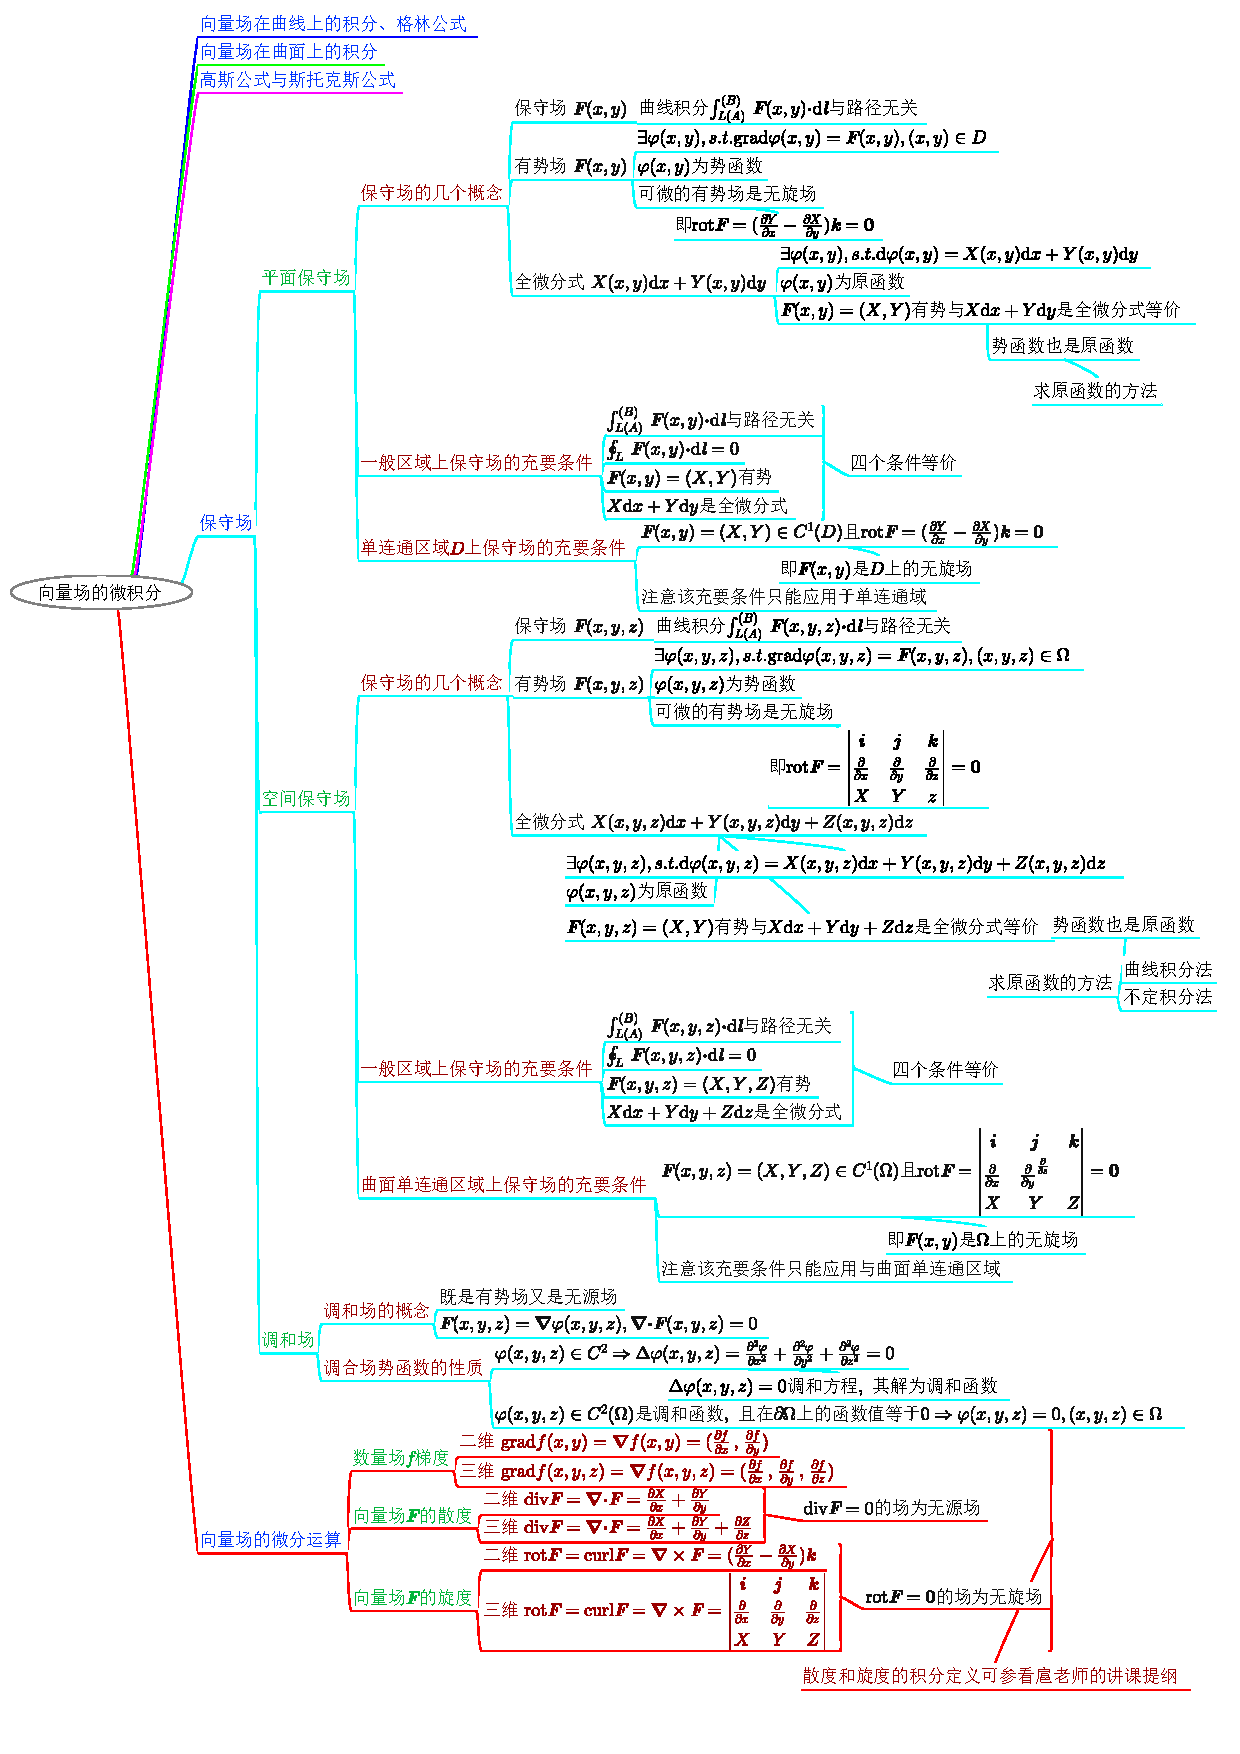
\includegraphics[height=1\textheight]{20190614.pdf}
\end{center}
\end{figure}
\subsection{保守场}

平面保守场的性质如下所示。

\begin{figure}[H]
\begin{center}
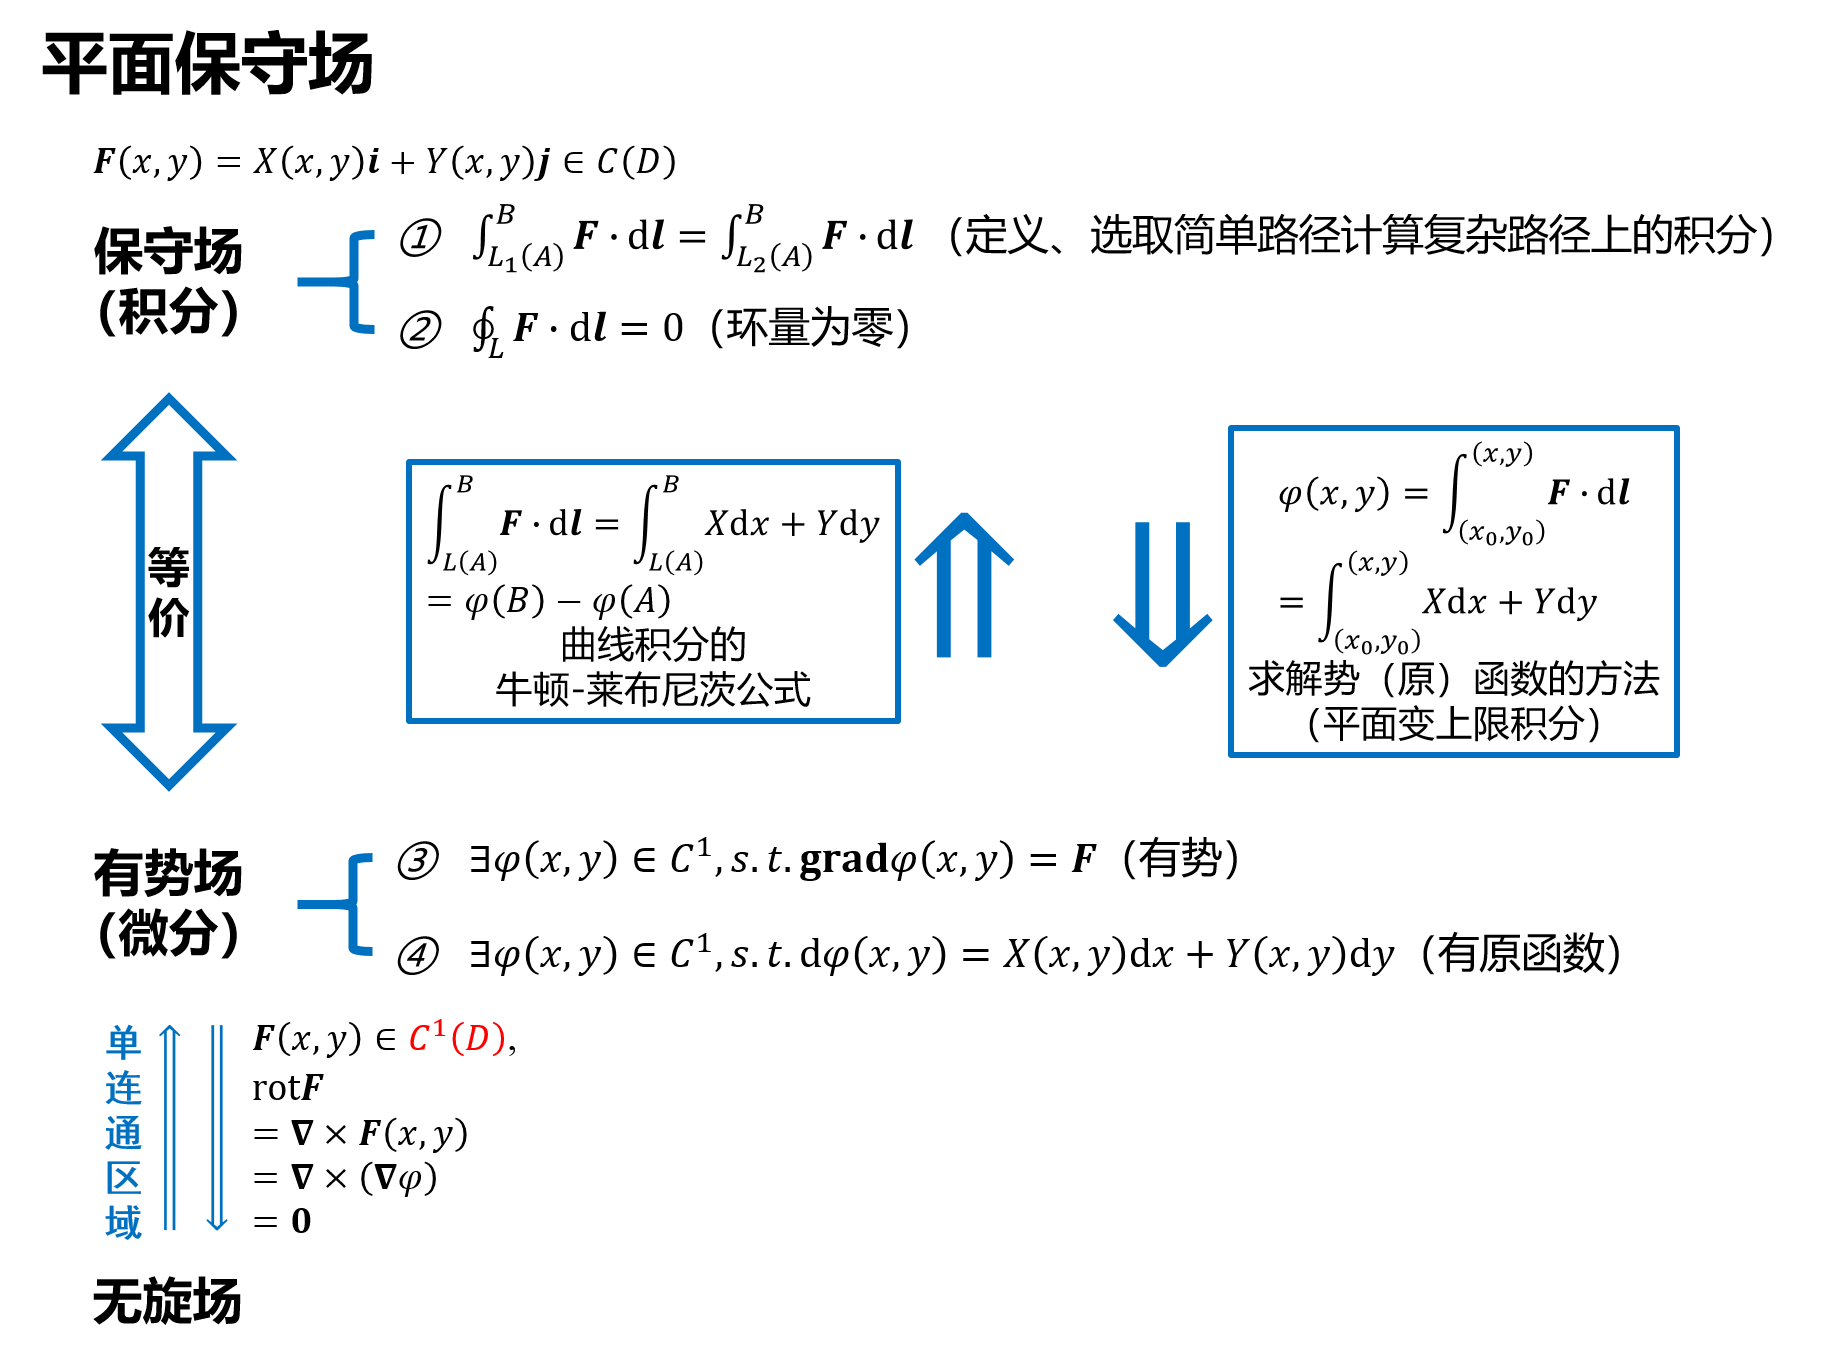
\includegraphics[height=0.54\textheight]{Figures25/PlaneConserv.png}
\end{center}
\end{figure}

\noindent{\bf说明:}
\begin{enumerate}
\item性质\textcircled{1}中的简单路径可选为与坐标轴平行的直线或折线路径. 

\begin{figure}[H]
\begin{center}
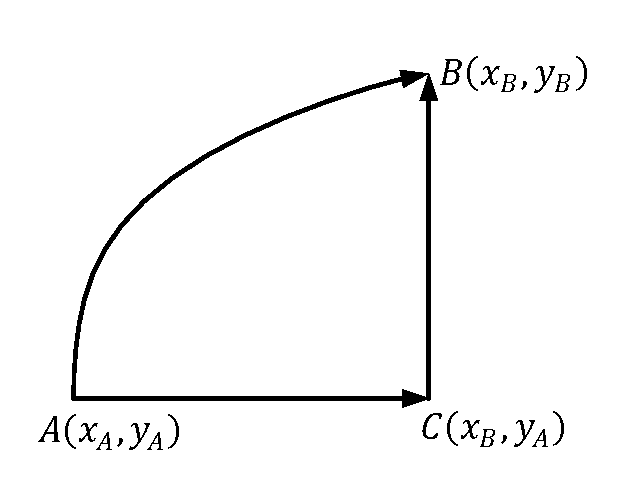
\includegraphics[height=0.25\textheight]{Figures25/Fig13-6-Intro-2.pdf}
\end{center}
\caption{与坐标轴平行的折线路径.}
\label{13-6-Intro}
\end{figure}

在与$x$轴平行的直线路径$AC$上,积分$\varint_{L(A)}^C{\bm F\bm\cdot\md\bm l}=\varint_{L(A)}^C{X(x,y)\md x+Y(x,y)\md y}$的被积表达式$X(x,y)\md x+Y(x,y)\md y$中$\md y=0,y=y_A$,故
\[\varint\nolimits_{L(A)}\nolimits^C{\bm F\bm\cdot\md\bm l}=\varint\nolimits_{(x_A,y_A)}\nolimits^{(x_B,y_A)}{X(x,y)\md x+Y(x,y)\md y}=\Int{x_A}{x_B}{X(x,y_A)}x.\]
在与$y$轴平行的直线路径$CB$上,积分$\varint_{L(C)}^B{\bm F\bm\cdot\md\bm l}=\varint_{L(C)}^B{X(x,y)\md x+Y(x,y)\md y}$的被积表达式$X(x,y)\md x+Y(x,y)\md y$中$\md x=0,x=x_B$,故
\[\varint\nolimits_{L(C)}\nolimits^B{\bm F\bm\cdot\md\bm l}=\varint\nolimits_{(x_B,y_A)}\nolimits^{(x_B,y_B)}{X(x,y)\md x+Y(x,y)\md y}=\Int{y_A}{y_B}{Y(x_B,y)}y.\]
【考察这一点的习题:1.(1)/(2)/(3)/(4),3.(1)/(2). (第一类题目)】
%\begin{figure}[H]
%\centering 
%\subfigure[] { \label{13-6-Intro-1} 
%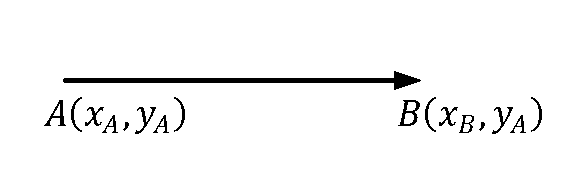
\includegraphics[height=0.1\textheight]{Figures25/Fig13-6-Intro-1.pdf} } 
%\subfigure[] { \label{13-6-Intro-2} 
%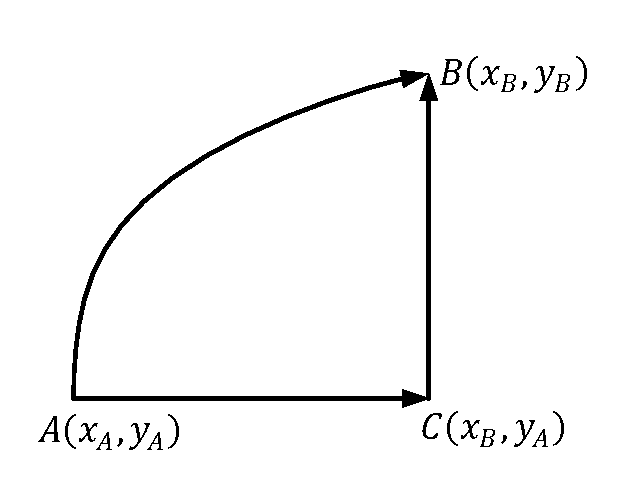
\includegraphics[height=0.3\textheight]{Figures25/Fig13-6-Intro-2.pdf} } 
%\caption{与坐标轴平行的直线或折线路径.} 
%\label{13-6-Intro} 
%\end{figure} 
\item\textcircled{1},\textcircled{2},\textcircled{3},\textcircled{4}相互等价,既是性质定理也是判定定理,知道其中一个即可判定该向量场是保守场,也就可以得到另外三个性质.
\item保守场是有势场,有势场也是保守场,二者是完全等价的概念. 保守场的两个性质从积分角度描述了向量场,有势场的两个性质从微分角度描述了向量场.
\item可通过对势函数这样一个数量场的分析来对向量场进行分析,比如可以用引力势能分析引力场,用重力势能分析重力场,用电势能分析电场力的场,用电势分析电场。
\item势函数与原函数相同.
\item可微的保守场是无旋场(但无旋场不一定是保守场). 

【考察这一点的习题:2. (第二类题目)】
\item平面单连通域上的无旋场是保守场. 常利用平面单连通区域上无旋来判定一个向量场是保守场.

【考察这一点的习题:1.(1)/(2)/(3)/(4),3.(1)/(2). (第一类题目)】

\item可微场才可用旋度算子计算旋度. 如一个向量场不可微,则不可用旋度算子计算旋度,难以用旋度为零来判断该向量场是保守场.

【考察这一点的习题:4. (第三类题目)】

\item求解全微分式的原函数有两种方法,变上限积分法和不定积分法.

【考察这一点的习题:3.(1)/(2). (第四类题目)】
\item空间保守场的性质与平面保守场类似,主要的不同是三维空间中的曲面单连通域(比如球壳是曲面单连通域,圆环体则不是曲面单连通域)上的无旋场是保守场。
\end{enumerate}
\subsection{无源场、无旋场}
\begin{enumerate}
\item无源场$\text{div}\bm F=\bm\nabla\bm\cdot\bm F=0$.

【与无源场有关的题目:5,7,8.(1)/(2),9. (第五类题目)】

\item无旋场$\text{rot}\bm F=\bm\nabla\times\bm F=\bm0$.

【与无旋场有关的题目:6,10.(1)/(2). (第六类题目)】

【综合题目:9. (主要考察通量的概念、高斯公式、无源场)】
\end{enumerate}
\subsection{向量场的微分运算习题分类}
\begin{enumerate}
\item验证三个算子的性质.

【习题13.1中的1., 2., 4.】

\item求梯度、散度、旋度.

【习题13.1中的3., 5., 6.】
\end{enumerate}
\subsection{习题13.6解答}
\begin{enumerate}
\item利用积分域与路线无关的性质计算下列积分:\\
(1)$\BLInt L{(x^3+xy^2)\md x+(y^3+x^2y)\md y}$,其中$L$为从$O(0,0)$经$A(1,1)$到$B(2,0)$的折线;\\
(2)$\BLInt L{(y+1)\tan x\md x-\ln\cos x\md y}$,其中$L$为曲线$x=\cos t,y=2\sin t(0\leqslant t\leqslant\pi)$,顺时针方向;\\
(3)$\BLInt L{(\ln\frac yx-1)\md x+\frac xy\md y}$,其中$L$为由点$A(1,1)$出发到$B(\me,3\me)$的任何一条不与$x$轴以及$y$轴相交的曲线;\\
(4)$\BLInt L{\frac{1+y^2f(xy)}y\md x+\frac x{y^2}[y^2f(xy)-1]\md y}$,其中$L$为由点$A(0,1)$出发到$B(1,2)$的任何一条不与$x$轴相交的曲线,$f$是连续可微的函数.

解:(1)\begin{figure}[H]
\begin{center}
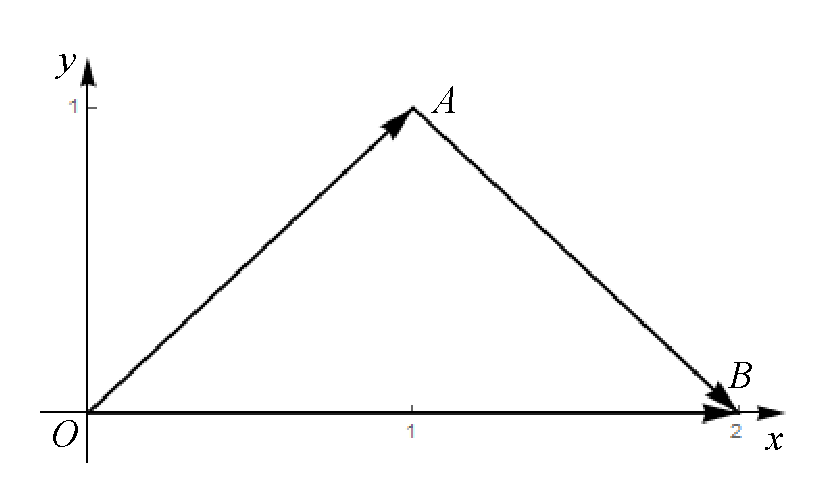
\includegraphics[height=0.2\textheight]{Figures25/Fig13-6-1-1.pdf}
\end{center}
\caption{习题13.6 1.(1)题图示}
\label{13-6-1-1}
\end{figure}

令$\begin{cases}
X(x,y)=x^3+xy^2,\\
Y(x,y)=y^3+x^2y,
\end{cases}$则$\bm F(x,y)=(X,Y)\in C^1(\mathbb R)$, 

$\because\mathbb R$为单连通域,

且$\text{rot}\bm F=(\pp Yx-\pp Xy)\bm k=(2xy-2xy)\bm k=\bm0$,

$\therefore\BLInt L{X\md x+Y\md y}=\varint_{(0,0)}^{(2,0)}{X\md x+Y\md y}=\Int02{x^3}x=\frac14x^4\big|_0^2=4$.

(2)\begin{figure}[H]
\begin{center}
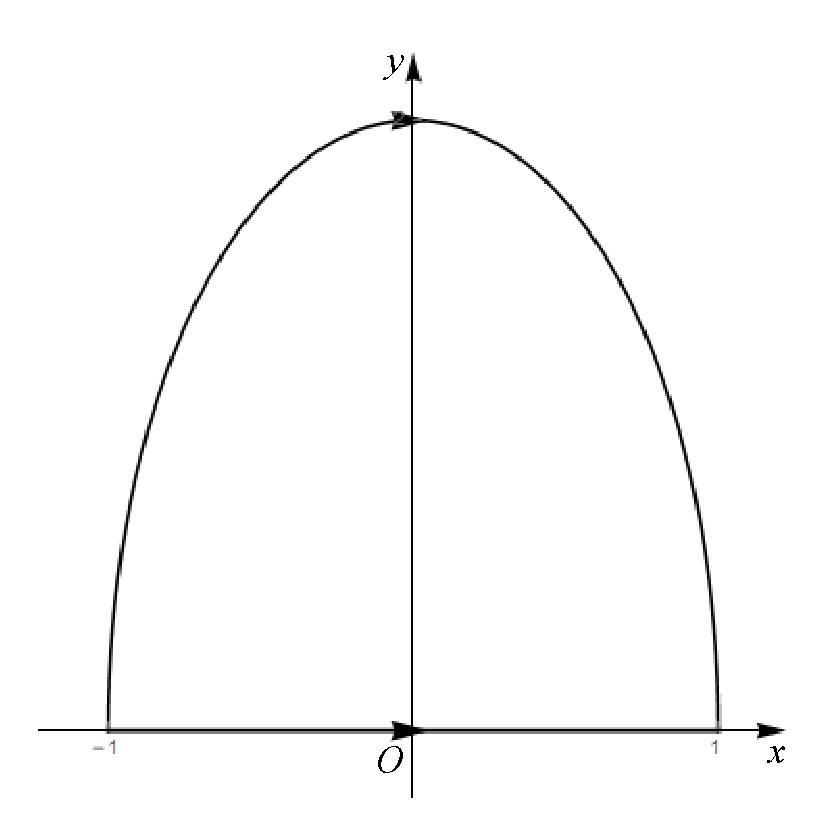
\includegraphics[height=0.3\textheight]{Figures25/Fig13-6-1-2.pdf}
\end{center}
\caption{习题13.6 1.(2)题图示}
\label{13-6-1-2}
\end{figure}

曲线$L:\begin{cases}
x=\cos t,\\
y=2\sin t,
\end{cases}(0\leqslant t\leqslant\pi)$为一椭圆弧$x^2+\frac{y^2}4=1,y\geqslant0$,顺时针的起点为$(-1,0)$终点为$(1,0)$,

设$D=(-\frac\pi2,\frac\pi2)\times(-\infty,\infty)$,则$L\in D$,

令$\begin{cases}
X(x,y)=(y+1)\tan x,\\
Y(x,y)=-\ln\cos x,
\end{cases}$则$\bm F(x,y)=(X,Y)\in C^1(D)$,

$\because D$是单连通区域,

且$\text{rot}\bm F=(\pp Yx-\pp Xy)\bm k=(-\frac{-\sin x}{\cos x}-\tan x)\bm k=\bm0$,

$\therefore\BLInt L{X\md x+Y\md y}=\varint_{(-1,0)}^{(1,0)}{X\md x+Y\md y}=\Int{-1}1{\tan x}x=0$.

(3)
\begin{figure}[H]
\begin{center}
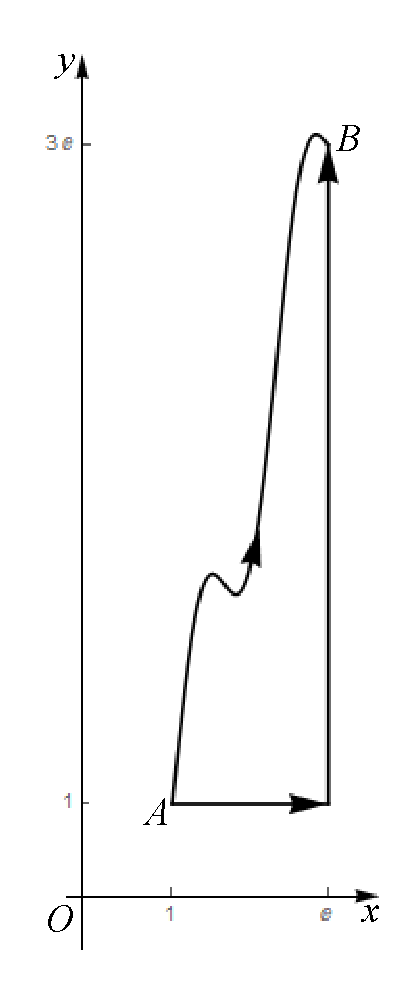
\includegraphics[height=0.5\textheight]{Figures25/Fig13-6-1-3.pdf}
\end{center}
\caption{习题13.6 1.(3)题图示}
\label{13-6-1-3}
\end{figure}

设$D=\Set{(x,y)}{x>0,y>0}$,则$L\in D$,

令$\begin{cases}
X(x,y)=\ln\frac yx-1,\\
Y(x,y)=\frac xy,
\end{cases}$则$\bm F(x,y)=(X,Y)\in C^1(D)$,

$\because D$是单连通域,

且$\text{rot}\bm F=(\pp Yx-\pp Xy)\bm k=(\frac1y-\frac1{\frac yx}\frac1x)\bm k=\bm0$,

$\therefore\BLInt L{X\md x+Y\md y}=\varint_{(1,1)}^{(\me,3\me)}{X\md x+Y\md y}=\varint_{(1,1)}^{(\me,1)}{X\md x+Y\md y}+\varint_{(\me,1)}^{(\me,3\me)}{X\md x+Y\md y}\\
=\Int1\me{(\ln\frac1x-1)}x+\Int1{3\me}{\frac\me y}y=x(-\ln x-1)\big|_1^\me-\Int1\me x{(-\ln x-1)}+\me\ln y\big|_1^{3\me}\\
=\me(-1-1)-1\cdot(0-1)+\Int1\me{x\frac1x}x+\me\ln{3\me}-0=-2\me+1+(\me-1)+\me\ln3+\me=\me\ln3$.

(4)
\begin{figure}[H]
\begin{center}
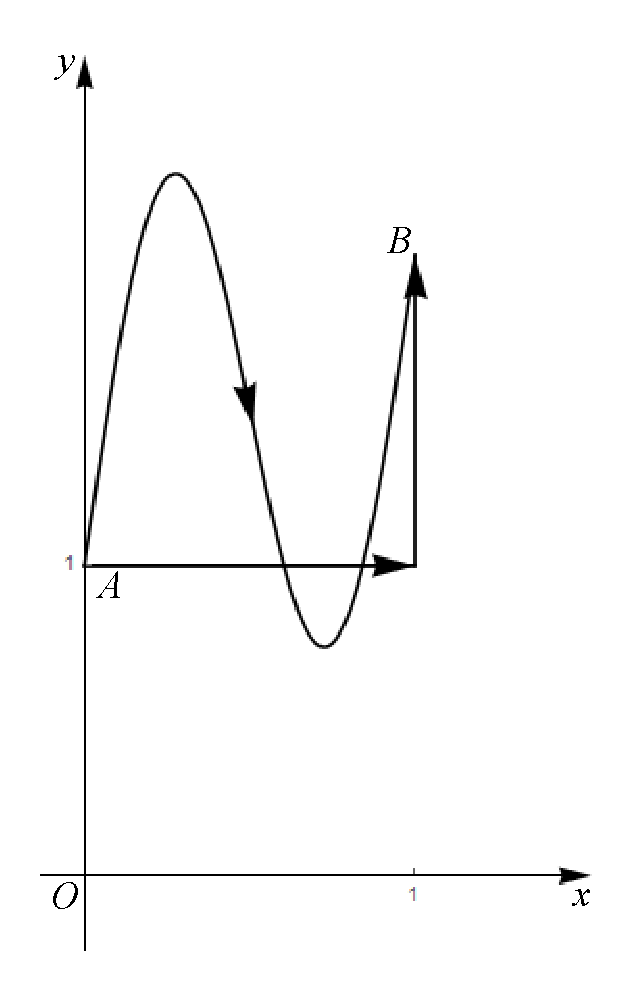
\includegraphics[height=0.5\textheight]{Figures25/Fig13-6-1-4.pdf}
\end{center}
\caption{习题13.6 1.(4)题图示}
\label{13-6-1-4}
\end{figure}

设$D=\Set{(x,y)}{y>0}$,

令$\begin{cases}
X(x,y)=\frac{1+y^2f(xy)}y=\frac1y+yf(xy),\\
Y(x,y)=\frac x{y^2}[y^2f(xy)-1]=xf(xy)-\frac x{y^2},
\end{cases}$则$\bm F(x,y)=(X,Y)\in C^1(D)$,

$\because D$单连通,

且$\text{rot}\bm F=(\pp Yx-\pp Xy)\bm k=\{f(xy)+xf'(xy)y-\frac1{y^2}-[-\frac1{y^2}+f(xy)+yf'(xy)x]\}\bm k=\bm0$,

$\therefore\BLInt L{X\md x+Y\md y}=\varint_{(0,1)}^{(1,2)}{X\md x+Y\md y}=\varint_{(0,1)}^{(1,1)}{X\md x+Y\md y}+\varint_{(1,1)}^{(1,2)}{X\md x+Y\md y}\\
=\Int01{[1+f(x)]}x+\Int12{[f(y)-\frac1{y^2}]}y=\Int01{}x+\Int01{f(x)}x+\Int12{f(y)}y-\Int12{\frac1{y^2}}y\\
=1+\Int02{f(x)}x+\frac1y\big|_1^2=\frac12+\Int02{f(x)}x$.

\item确定$p$的值,使积分$\varint_A^B{(x^4+4xy^p)\md x+(6x^{p-1}y^2-5y^4)\md y}$与路线无关. 当$A=(0,0),B=(1,2)$时,计算积分的值.

\begin{figure}[H]
\begin{center}
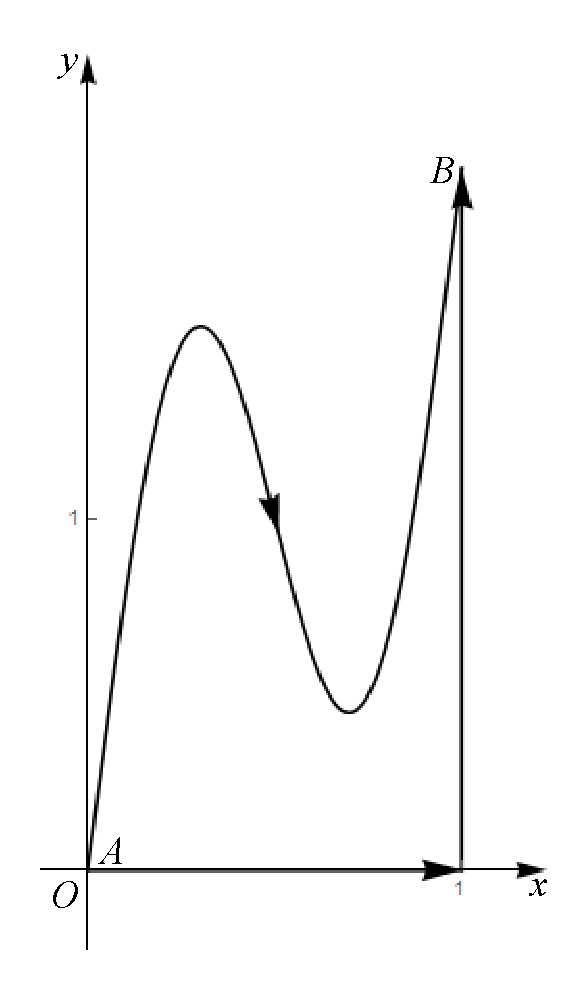
\includegraphics[height=0.5\textheight]{Figures25/Fig13-6-2.pdf}
\end{center}
\caption{习题13.6 2.题图示}
\label{13-6-2}
\end{figure}

解:$\because$积分$\varint_A^B{(x^4+4xy^p)\md x+(6x^{p-1}y^2-5y^4)\md y}$与路线无关,

令$\begin{cases}
X(x,y)=x^4+4xy^p,\\
Y(x,y)=6x^{p-1}y^2-5y^4,
\end{cases}$则$\bm F(x,y)=(X,Y)$是保守场,

$\because\bm F(x,y)\in C^1$,

$\therefore\text{rot}\bm F=(\pp Yx-\pp Xy)\bm k=[6(p-1)x^{p-2}y^2-4pxy^{p-1}]\bm k=\bm0$,

$\therefore p=3$.

$\because A=(0,0),B=(1,2)$,

$\therefore\varint_A^B{X\md x+Y\md y}=\varint_{(0,0)}^{(1,2)}{X\md x+Y\md y}=\varint_{(0,0)}^{(1,0)}{X\md x+Y\md y}+\varint_{(1,0)}^{(1,2)}{X\md x+Y\md y}\\
=\Int01{x^4}x+\Int02{(6y^2-5y^4)}y=\frac15x^5\big|_0^1+(2y^3-y^5)\big|_0^2=\frac15+(2\cdot8-32)=-\frac{79}5$.

\item判定下列微分形式是否为全微分,若是,求出其原函数:\\
(1)$(2x\cos y-y^2\sin x)\md x+(2y\cos x-x^2\sin y)\md y$;\\
(2)$(\me^x\cos y+2xy^2)\md x+(2x^2y-\me^x\sin y)\md y$.

解:(1)令$\begin{cases}
X(x,y)=2x\cos y-y^2\sin x,\\
Y(x,y)=2y\cos x-x^2\sin y,
\end{cases}$则$\bm F(x,y)=(X,Y)\in C^1(\mathbb R)$,

$\because\mathbb R$是单连通区域,

且$\text{rot}\bm F=[\pp Yx-\pp Xy)\bm k=(-2y\sin x-2x\sin y-(-2x\sin y-2y\sin x)]\bm k=\bm0$,

$\therefore X\md x+Y\md y$是全微分式,

方法1:原函数$\varphi(x,y)=\varint_{(0,0)}^{(x,y)}{X(s,t)\md s+Y(s,t)\md t}+C\\
=\varint_{(0,0)}^{(x,0)}{X(s,t)\md s+Y(s,t)\md t}+\varint_{(x,0)}^{(x,y)}{X(s,t)\md s+Y(s,t)\md t}+C\\
=\Int0x{2s}s+\Int0y{(2t\cos x-x^2\sin t)}t+C=s^2\big|_0^x+(t^2\cos x+x^2\cos t)\big|_0^y\\
=x^2+(y^2\cos x-x^2\sin y-x^2)+C=y^2\cos x-x^2\sin y+C$.

方法2:设原函数为$\varphi(x,y)$,

则$\pp{\varphi(x,y)}x=2x\cos y-y^2\sin x$,

$\therefore\varphi(x,y)=x^2\cos y+y^2\cos x+C(y)$,

$\therefore\pp{\varphi(x,y)}y=-x^2\sin y+2y\cos x+C'(y)=2y\cos x-x^2\sin y$,

$\therefore C'(y)=0,\ C(y)=C$,

$\therefore\varphi(x,y)=x^2\cos y+y^2\cos x+C$.

(2)令$\begin{cases}
X(x,y)=\me^x\cos y+2xy^2,\\
Y(x,y)=2x^2y-\me^x\sin y,
\end{cases}$则$\bm F(x,y)=(X,Y)\in C^1(\mathbb R)$,

$\because\mathbb R$是单连通区域,

且$\text{rot}\bm F=(\pp Yx-\pp Xy)\bm k=[4xy-\me^x\sin y-(-\me^x\sin y+4xy)]\bm k=\bm0$,

$\therefore X\md x+Y\md y$是全微分式.

方法1:原函数$\varphi(x,y)=\varint_{(0,0)}^{(x,y)}{X(s,t)\md s+Y(s,t)\md t}+C_1\\
=\varint_{(0,0)}^{(x,0)}{X(s,t)\md s+Y(s,t)\md t}+\varint_{(x,0)}^{(x,y)}{X(s,t)\md s+Y(s,t)\md t}+C_1\\
=\Int0x{\me^s}s+\Int0y{(2x^2t-\me^x\sin t)}t+C_1=\me^s\big|_0^x+(x^2t^2+\me^x\cos t)\big|_0^y+C_1\\
=\me^x-1+(x^2y^2+\me^x\cos y-\me^x)+C_1=x^2y^2+\me^x\cos y+C$.

方法:设原函数为$\varphi(x,y)$,

则$\pp{\varphi(x,y)}x=\me^x\cos y+2xy^2$,

$\therefore\varphi(x,y)=\me^x\cos y+x^2y^2+C(y)$,

$\therefore\pp{\varphi(x,y)}y=-\me^x\sin y+2x^2y+C'(y)=2x^2y-\me^x\sin y$,

$\therefore C'(y)=0,C(y)=C$,

$\therefore\varphi(x,y)=\me^x\cos y+x^2y^2+C$.

\item设$f(u)$连续,$L$为逐段光滑简单闭曲线,求证:
\[
\BLOInt L{f(x^2+y^2)(x\md x+y\md y)}=0.
\]
证明:令$\varphi(x,y)=\frac12\Int0{x^2+y^2}{f(u)}u$,

$\pp\varphi x=f(x^2+y^2)x,\pp\varphi y=f(x^2+y^2)y$,

$\therefore\md\varphi(x,y)=\pp\varphi x\md x+\pp\varphi y\md y=f(x^2+y^2)(x\md x+y\md y)$,

$\therefore\BLOInt L{f(x^2+y^2)(x\md x+y\md y)}=0$.

5.设一元函数$f$有连续的导数,计算$\bm\nabla\bm\cdot(f(r)\bm r)$,其中
\[
\bm r=x\bm i+y\bm j+z\bm k,\ r=\sqrt{x^2+y^2+z^2},
\]
并说明$f$满足什么条件时,$f(r)\bm r$为无源场.

解:$\bm\nabla\bm\cdot(f(r)\bm r)=(\ppx{},\ppy{},\ppz{})\bm\cdot(xf(r),yf(r),zf(r))=\pp{[xf(r)]}x+\pp{[yf(r)]}y+\pp{[zf(r)]}z\\
=f(r)+xf'(r)\frac xr+f(r)+yf'(r)\frac yr+f(r)+zf'(r)\frac zr\\
=3f(r)+f'(r)\frac{x^2+y^2+z^2}r=3f(r)+rf'(r)$.

$\because f(r)\bm r$无源,

$\therefore 3f(r)+rf'(r)=0$,

当$f(r)\not\equiv0$时$\frac{\md f(r)}{f(r)}=-\frac3r\md r$,

$\therefore\ln|f(r)|=-3\ln|r|+C$,

$\therefore f(r)r^3=\pm\me^C$,

$\therefore f(r)r^3=C_0,\ C_0,C$为任意常数,$f(r)\equiv0$也满足该式.

\item设$\bm F=f(r)\bm r$($r$与$\bm r$的意义与上题同),证明$\text{rot}\bm F=\bm0$.

证明:$\text{rot}\bm F=\bm\nabla\times\bm F=\begin{vmatrix}
\bm i&\bm j&\bm k\\
\ppx{}&\ppy{}&\ppz{}\\
xf(r)&yf(r)&zf(r)
\end{vmatrix}\\
=(\ppy{zf(r)}-\ppz{yf(r)},\ppz{xf(r)}-\ppx{zf(r)},\ppx{yf(r)}-\ppy{xf(r)})\\
=(zf'(r)\frac yr-yf'(r)\frac zr,xf'(r)\frac zr-zf'(r)\frac xr,yf'(r)\frac yr-xf'(r)\frac yr)\\
=(0,0,0)=\bm0$.

\item设$f$有连续的二阶导数,计算$\bm\nabla\bm\cdot(\bm\nabla f(r))$,其中$r,\bm r$同题5,并说明$f$满足什么条件时,$\nabla f$为无源场.

解:$\bm\nabla\bm\cdot(\bm\nabla f(r))=\bm\nabla\bm\cdot(f'(r)\frac xr,f'(r)\frac yr,f'(r)\frac zr)=\varppx{[f'(r)\frac xr]}+\varppy{[f'(r)\frac yr]}+\varppz{[f'(r)\frac zr]}\\
=f''(r)\frac xr\cdot\frac xr+f'(r)\frac{r-x\frac xr}{r^2}+f''(r)\frac yr\cdot\frac yr+f'(r)\frac{r-y\frac yr}{r^2}+f''(r)\frac zr\cdot\frac zr+f'(r)\frac{r-z\frac zr}{r^2}\\
=f''(r)\frac{x^2}{r^2}+f'(r)\frac{y^2+z^2}{r^3}+f''(r)\frac{y^2}{r^2}+f'(r)\frac{z^2+x^2}{r^3}+f''(r)\frac{z^2}{r^2}+f'(r)\frac{x^2+y^2}{r^3}\\
=f''(r)\frac{x^2+y^2+z^2}{r^2}+f'(r)\frac{2(x^2+y^2+z^2)}{r^3}=f''(r)+\frac2rf'(r)$.

$\because\nabla f$为无源场,

$\therefore f''(r)+\frac2rf'(r)=0$,

当$f'(r)\not\equiv0$时$\frac{\md f'(r)}{f'(r)}=-\frac2r\md r$,

$\therefore\ln|f'(r)|=-2\ln|r|+C$,

$\therefore f'(r)r^2=\pm\me^C$,

$\therefore f'(r)=\frac{C_0}{r^2}$,$f'(r)\equiv0$也满足该式.

$\therefore f(r)=-\frac{C_0}r+C_2=\frac{C_1}r+C_2$.

\item证明下列向量场为无源场:\\
(1)$\bm v=\bm u_1\times\bm u_2$,其中$\bm u_1,\bm u_2$是无旋场;\\
(2)$\bm v=\frac{\bm r}{r^3}$,其中$r,\bm r$同题5.

证明:(1)$\text{div}\bm v=\bm\nabla\bm\cdot\bm v=\bm\nabla\bm\cdot(\bm u_1\times\bm u_2)=\bm u_2\bm\cdot(\bm\nabla\times\bm u_1)-\bm u_1\bm\cdot(\bm\nabla\times\bm u_2)\\
=\bm u_2\bm\cdot\bm0-\bm u_1\bm\cdot\bm0=0-0=0$.

{\bf注:}该公式的证明见习题13.1中的2题.

(2)$\bm\nabla\bm\cdot\bm v=\bm\nabla\bm\cdot(\frac{\bm r}{r^3})=(\ppx{},\ppy{},\ppz{})\bm\cdot(\frac x{r^3},\frac y{r^3},\frac z{r^3})=\varppx{(\frac x{r^3})}+\varppy{(\frac y{r^3})}+\varppz{(\frac z{r^3})}\\
=\frac{r^3-x3r^3\frac xr}{r^6}+\frac{r^3-y3r^3\frac yr}{r^6}+\frac{r^3-z3r^3\frac zr}{r^6}=\frac{r^2-3x^2}{r^5}+\frac{r^2-3y^2}{r^5}+\frac{r^2-3z^2}{r^5}\\
=\frac{y^2+z^2-2x^2}{r^5}+\frac{z^2+x^2-2y^2}{r^5}+\frac{x^2+y^2-2z^2}{r^5}=0$.

9.求电场$\bm v=\frac{\bm r}{r^3}$穿过包围原点的任意简单光滑闭曲面的电通量,其中$r,\bm r$同题5.

解:设$S$是包围原点的任意简单光滑闭曲面,$S_1$是$S$围成区域中的包围原点的任意简单光滑闭曲面,$S_1,S$外侧为正,记$S,S_1^-$围成的区域为$\Omega$,

则$\BSOIInt S{\bm v\bm\cdot\md\bm S}-\BSOIInt{S_1}{\bm v\bm\cdot\md\bm S}=\BSOIInt S{\bm v\bm\cdot\md\bm S}+\BSOIInt{S_1^-}{\bm v\bm\cdot\md\bm S}=\BSOIInt{S+S_1^-}{\bm v\bm\cdot\md\bm S}$,

$\because\Omega$不包含原点,

$\therefore\bm v\in C^1(\Omega)$且由上述题8(2)可知$\bm\nabla\bm\cdot\bm v=0$,

$\therefore\BSOIInt{S+S_1^-}{\bm v\bm\cdot\md\bm S}=\IIInt\Omega{\bm\nabla\bm\cdot\bm v}V=\IIInt\Omega0V=0$,

$\therefore\BSOIInt S{\bm v\bm\cdot\md\bm S}=\BSOIInt{S_1}{\bm v\bm\cdot\md\bm S}$,

$\therefore\bm v=\frac{\bm r}{r^3}$穿过包围原点的任意简单光滑闭曲面的电通量都相等,故可取一个特殊的曲面计算电通量的值.

不妨取$S_1:r=a,a>0$,记$\Omega_1$是$S_1$围成的区域,

$\therefore\BSOIInt{S_1}{\bm v\bm\cdot\md\bm S}=\BSOIInt{S_1}{\frac{\bm r}{r^3}\bm\cdot\md\bm S}=\BSOIInt{S_1}{\frac{\bm r}{a^3}\bm\cdot\md\bm S}=\frac1{a^3}\BSOIInt{S_1}{\bm r\bm\cdot\md\bm S}=\frac1{a^3}\IIInt{\Omega_1}{\bm\nabla\bm\cdot\bm r}V\\
=\frac1{a^3}\IIInt{\Omega_1}{(\pp xx+\pp yy+\pp zz)}V=\frac1{a^3}\IIInt{\Omega_1}{3}V=\frac3{a^3}\IIInt{\Omega_1}{}V=\frac3{a^3}\frac43\pi a^3=4\pi$.\footnotemark\footnotetext{该题给出了真空中点电荷电场的高斯定理的证明. 真空中位于原点的点电荷$q$产生的电场
\[\bm E=\frac q{4\pi\varepsilon_0}\frac{\bm r}{r^3}=\frac q{4\pi\varepsilon_0}\bm v,\]

故该电场穿过包围该电荷的任意简单光滑闭曲面的电通量
\[\BSOIInt S{\bm E\bm\cdot\md\bm S}=\frac q{4\pi\varepsilon_0}\BSOIInt S{\bm v\bm\cdot\md\bm S}=\frac q{\varepsilon_0}.\]

即真空中的电荷的电场穿过包围该点电荷的任意简单光滑闭曲面的电通量与该电荷的电量成正比.

}

\begin{figure}[H]
\begin{center}
\subfigure[]{\label{13-6-9-1}{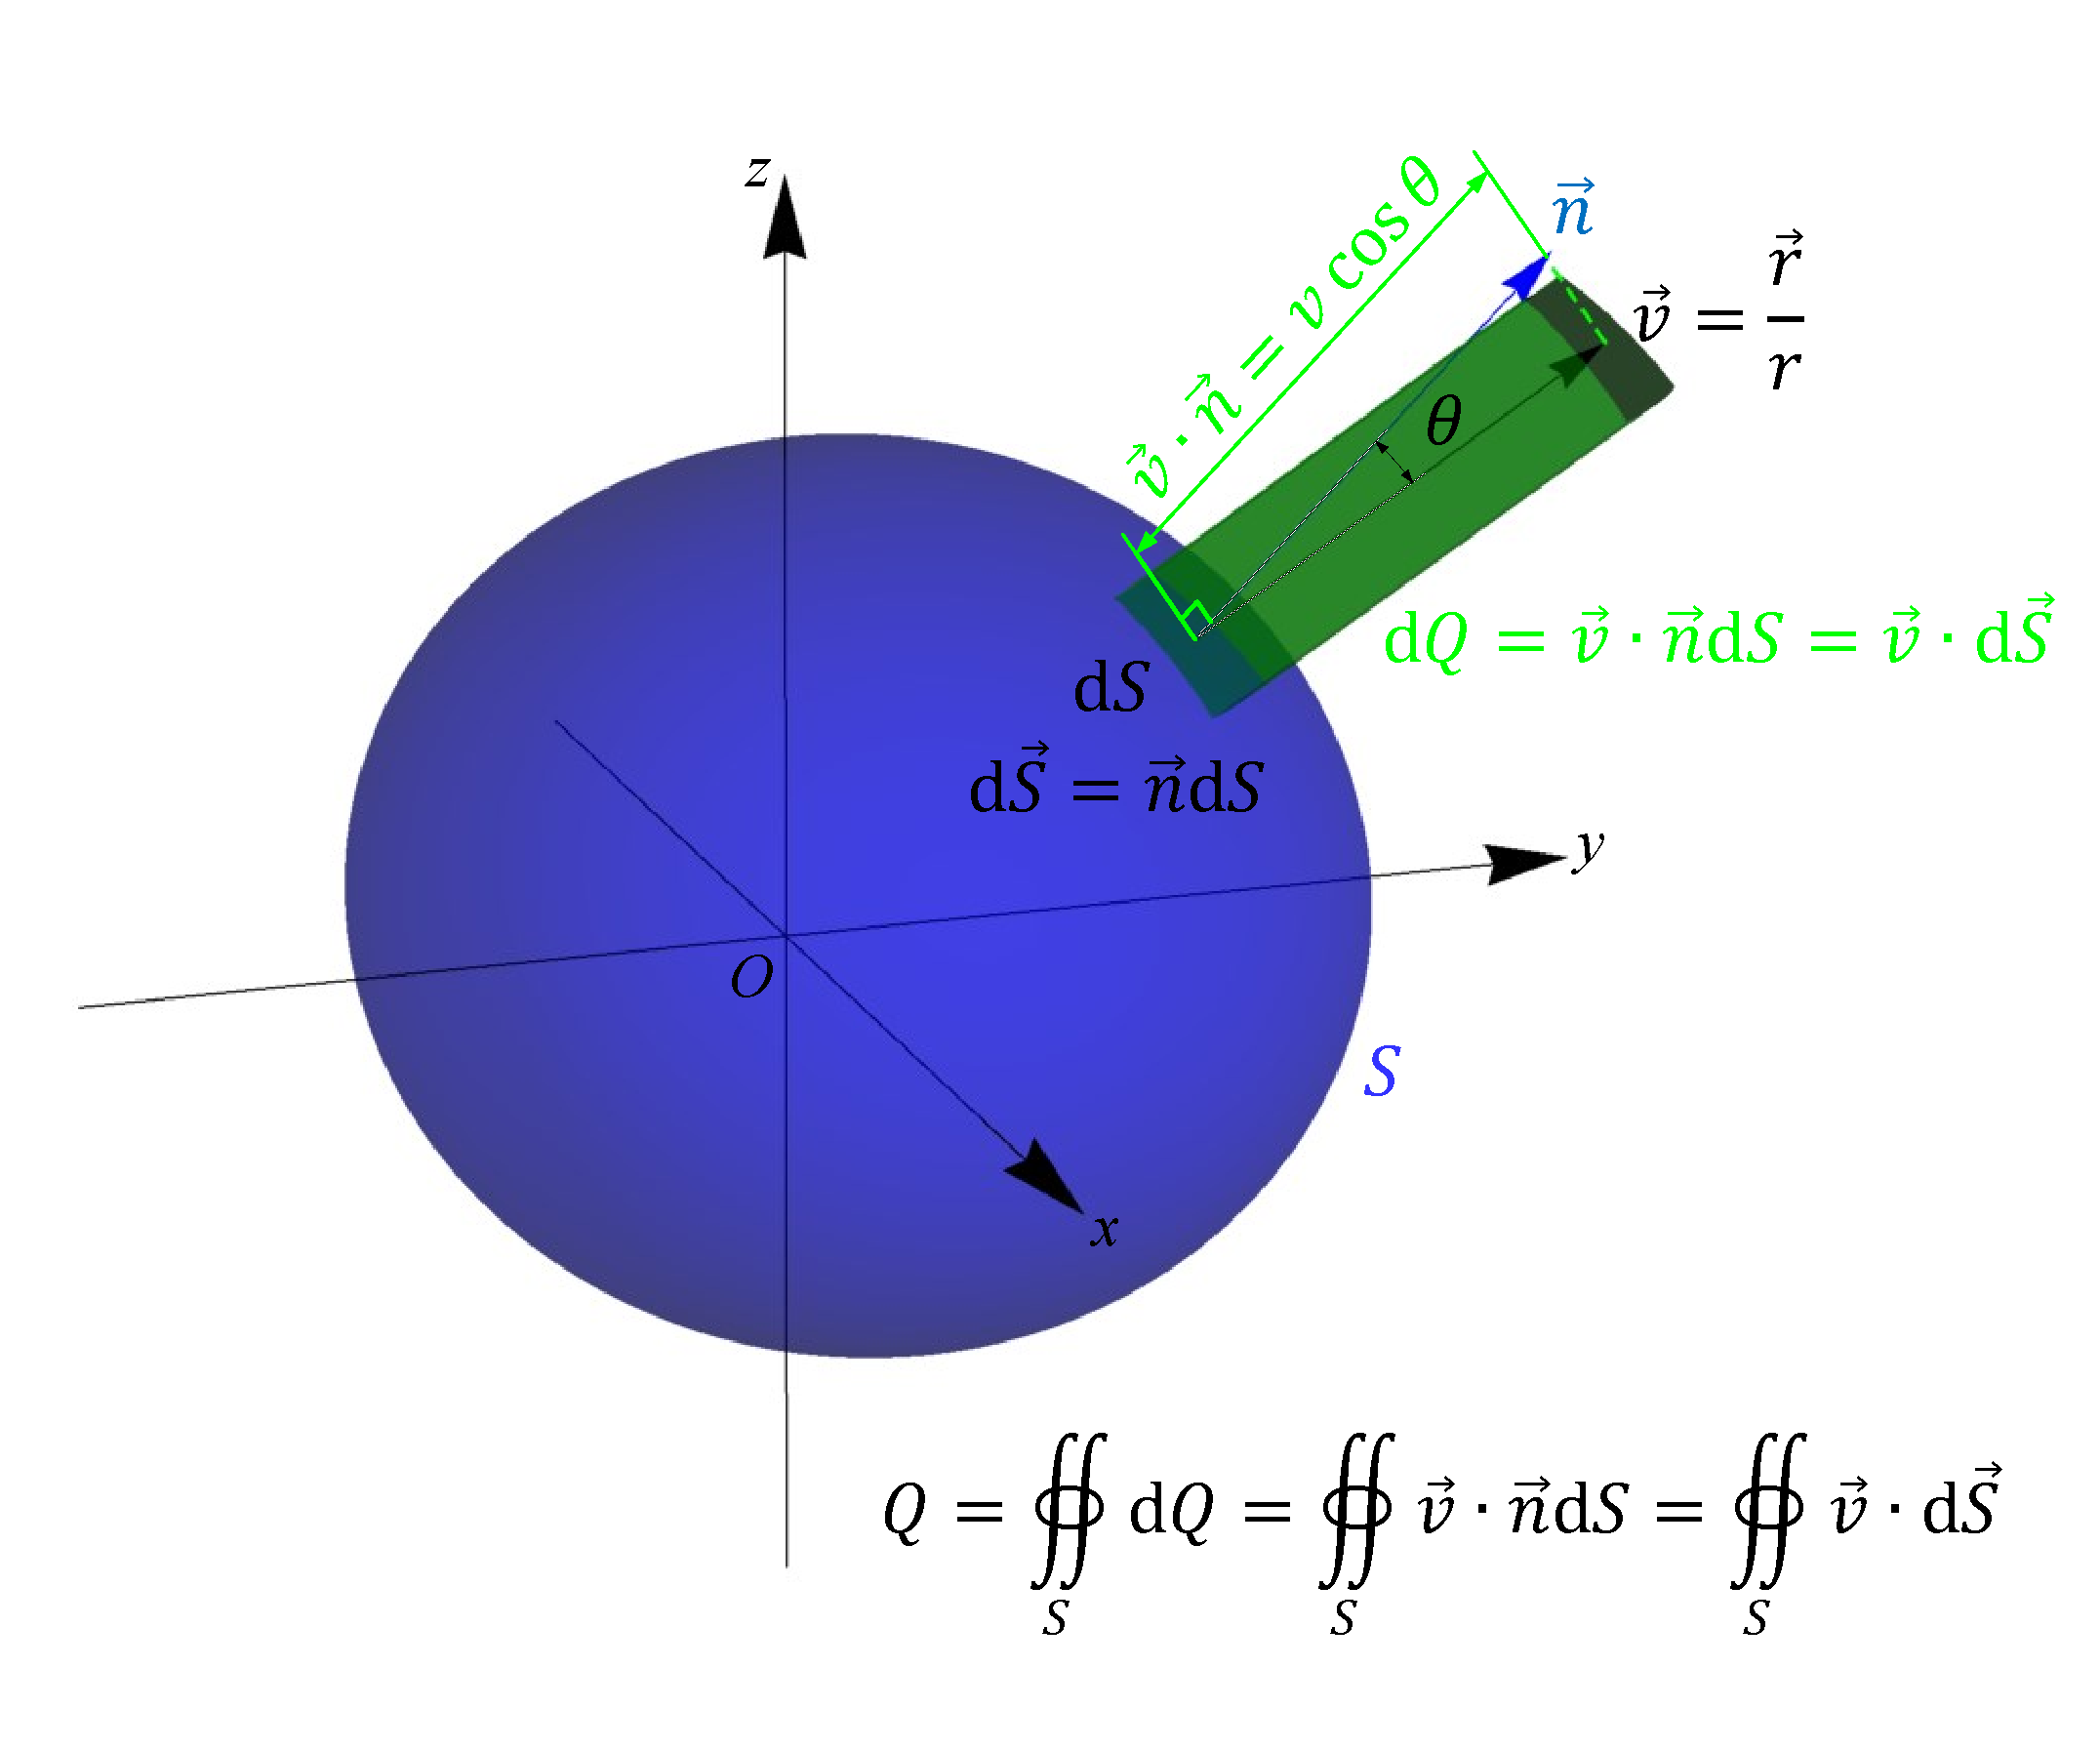
\includegraphics[height=0.58\textheight]{Figures25/Fig13-6-9-1.pdf} }}
\end{center}
\end{figure}
\addtocounter{figure}{-1}
\begin{figure}[H]
\addtocounter{figure}{1}
\begin{center}
\subfigure[]{\label{13-6-9-2} {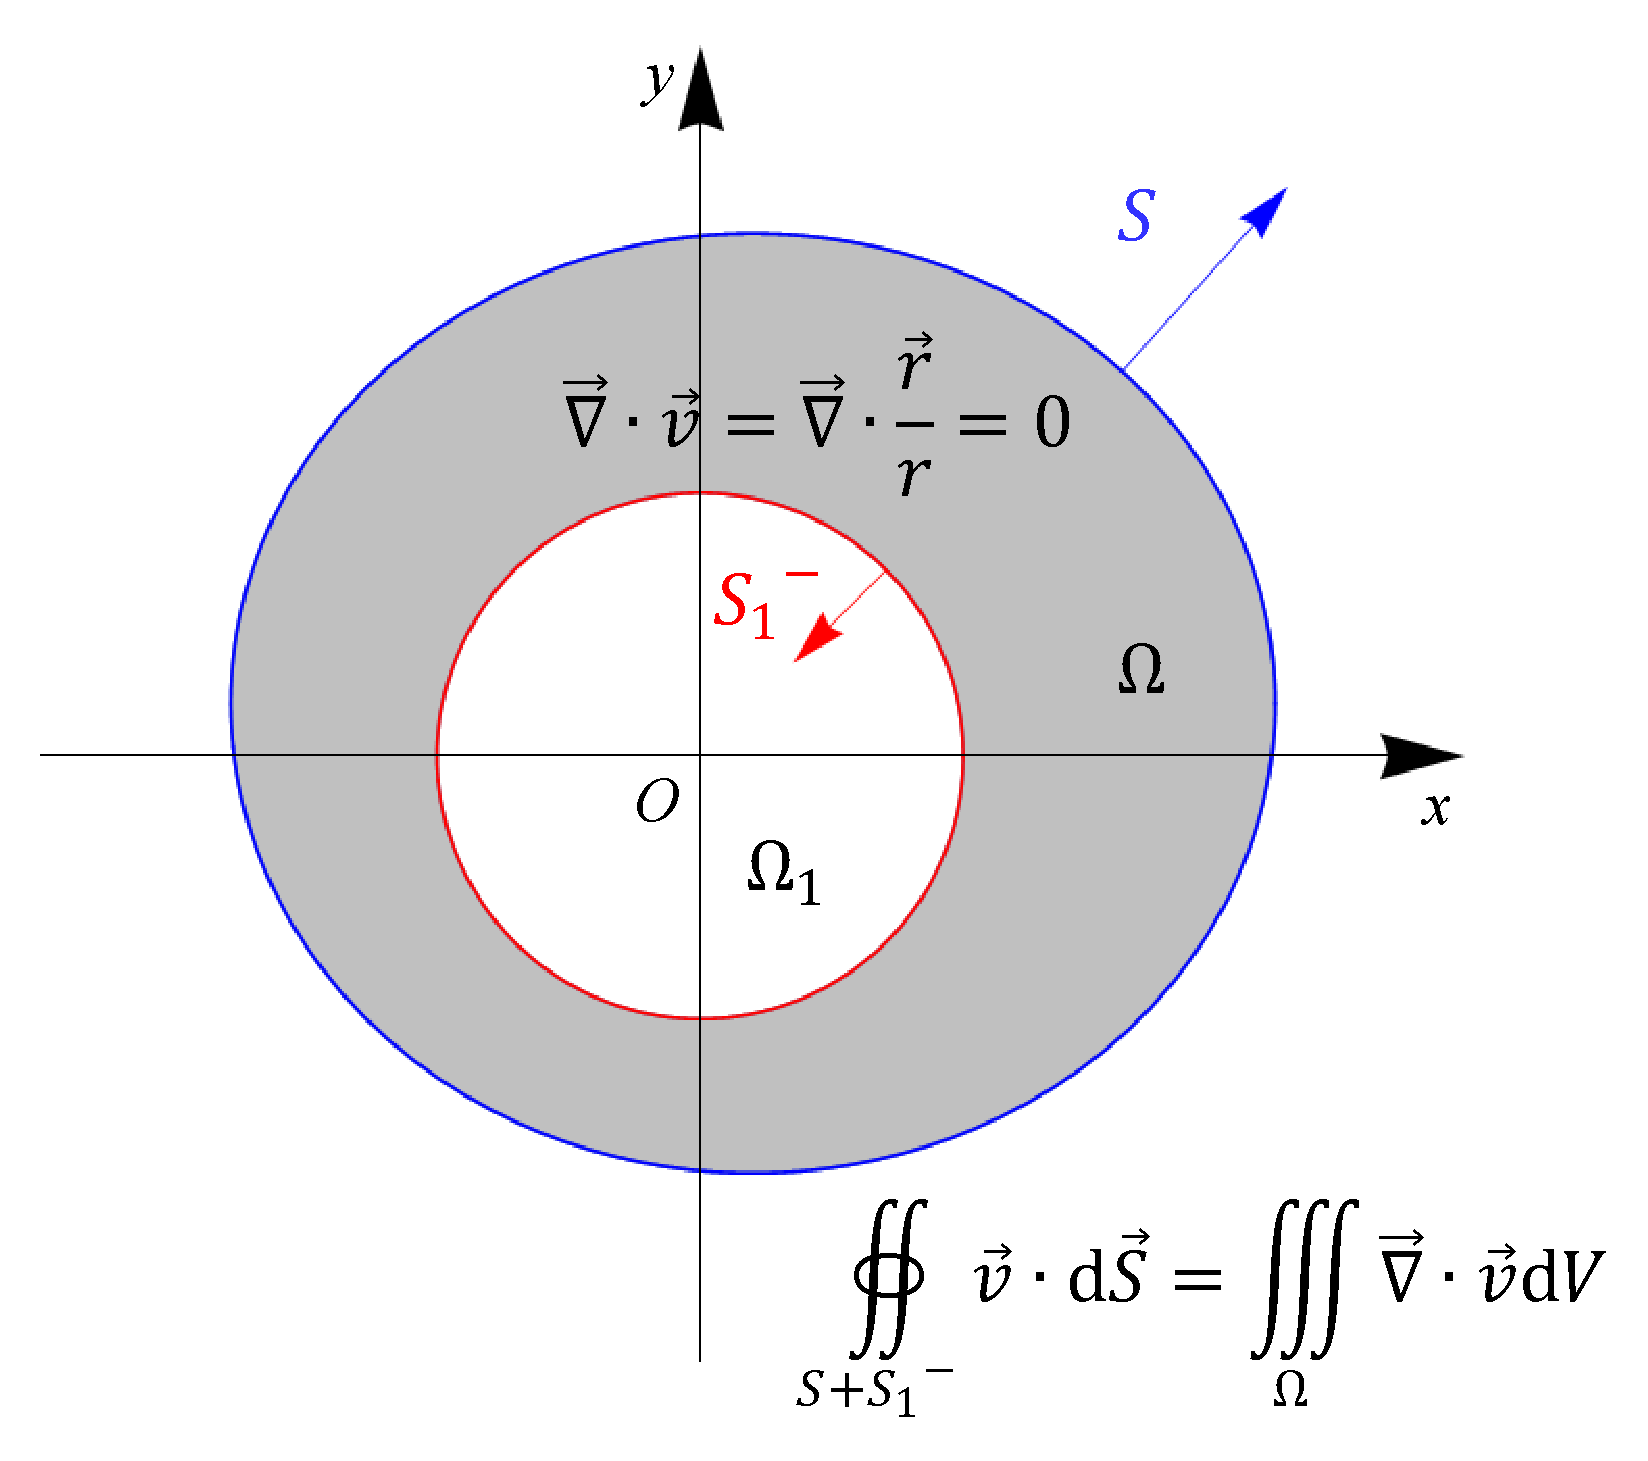
\includegraphics[height=0.6\textheight]{Figures25/Fig13-6-9-2.pdf} }}
\end{center}
\caption{习题13.6 9.题图示}
\label{13-6-9}
\end{figure}

\item证明下列向量场为无旋场:\\
(1)$\bm v=(x-x_0)\bm i+(y-y_0)\bm j+(z-z_0)\bm k$;\\
(2)$\bm v=yz(2x+y+z)\bm i+zx(x+2y+z)\bm j+xy(x+y+2z)\bm k$.

证明:(1)$\text{rot}\bm v=\bm\nabla\times\bm v=\begin{vmatrix}
\bm i&\bm j&\bm k\\
\ppx{}&\ppy{}&\ppz{}\\
x-x_0&y-y_0&z-z_0
\end{vmatrix}\\
=(\ppy{(z-z_0)}-\ppz{(y-y_0)},\ppz{(x-x_0)}-\ppx{(z-z_0)},\ppx{(y-y_0)}-\ppy{(x-x_0)})=(0,0,0)=\bm0$.

(2)$\bm v=(2xyz+y^2z+yz^2)\bm i+(zx^2+2xyz+xz^2)\bm j+(x^2y+xy^2+2xyz)\bm k$,
\[\begin{aligned}
\text{rot}\bm v&=\bm\nabla\times\bm v=\begin{vmatrix}
\bm i&\bm j&\bm k\\
\ppx{}&\ppy{}&\ppz{}\\
2xyz+y^2z+yz^2&zx^2+2xyz+xz^2&x^2y+xy^2+2xyz
\end{vmatrix}\\
&=(\ppy{(x^2y+xy^2+2xyz)}-\ppz{(zx^2+2xyz+xz^2)},\\
&\hspace{3cm}\ppz{(2xyz+y^2z+yz^2)}-\ppx{(x^2y+xy^2+2xyz)},\\
&\hspace{6cm}\ppx{(zx^2+2xyz+xz^2)}-\ppy{(2xyz+y^2z+yz^2)})\\
&=(x^2+2xy+2xz-(x^2+2xy+2zx),\\
&\hspace{3cm}2xy+y^2+2yz-(2xy+y^2+2yz),\\
&\hspace{6cm}2zx+2yz+z^2-(2zx+2yz+z^2))\\
&=\bm0.
\end{aligned}\]
\end{enumerate}
\subsection{习题13.1解答}
\begin{enumerate}
\item验证梯度算子$\bm\nabla$的下列性质,其中$\alpha,\beta$为任意常数,$f,g$为任意可微函数:\\
(1)$\bm\nabla(\alpha f+\beta g)=\alpha\bm\nabla+\beta\bm\nabla g$;\\
(2)$\bm\nabla(fg)=g\bm\nabla f+f\bm\nabla g$;\\
(3)$\bm\nabla(\frac fg)=\frac{g\bm\nabla f-f\bm\nabla g}{g^2}$(在$g$不等于零处成立).

证明:(1)\[\begin{split}
\bm\nabla(\alpha f+\beta g)&=(\pp{}x\bm i+\pp{}y\bm j+\pp{}z\bm k)(\alpha f+\beta g)\\
&=\pp{(\alpha f+\beta g)}x\bm i+\pp{(\alpha f+\beta g)}y\bm j+\pp{(\alpha f+\beta g)}z\bm k\\
&=(\alpha\pp fx+\beta\pp gx)\bm i+(\alpha\pp fy+\beta\pp gy)\bm j+(\alpha\pp fz+\beta\pp gz)\bm k\\
&=\alpha(\pp fx\bm i+\pp fy\bm j+\pp fz\bm k)+\beta(\pp gx\bm i+\pp gy\bm j+\pp gz\bm k)\\
&=\alpha\bm\nabla f+\beta\bm\nabla g.
\end{split}\]
(2)\[\begin{split}
\bm\nabla(fg)&=(\pp{}x\bm i+\pp{}y\bm j+\pp{}z\bm k)(fg)\\
&=\pp{(fg)}x\bm i+\pp{(fg)}y\bm j+\pp{(fg)}z\bm k\\
&=(g\pp fx+f\pp gx)\bm i+(g\pp fy+f\pp gy)\bm j+(g\pp fz+f\pp gz)\bm k\\
&=g(\pp fx\bm i+\pp fy\bm j+\pp fz\bm k)+f(\pp gx\bm i+\pp gy\bm j+\pp gz\bm k)\\
&=g\bm\nabla f+f\bm\nabla g.
\end{split}\]
(3)\[\begin{split}
\bm\nabla(\frac fg)&=(\pp{}x\bm i+\pp{}y\bm j+\pp{}z\bm k)(\frac fg)\\
&=\pp{}x(\frac fg)\bm i+\pp{}y(\frac fg)\bm j+\pp{}z(\frac fg)\bm k\\
&=\frac{g\pp fx-f\pp gx}{g^2}\bm i+\frac{g\pp fy-f\pp gy}{g^2}\bm j+\frac{g\pp fz-f\pp gz}{g^2}\bm k\\
&=\frac{g(\pp fx\bm i+\pp fy\bm j+\pp fz\bm k)-f(\pp gx\bm i+\pp gy\bm j+\pp gz\bm k)}{g^2}\\
&=\frac{g\bm\nabla f-f\bm\nabla g}{g^2}.
\end{split}\]
\item验证散度算子的下列性质(其中$f$为函数,$\bm u,\bm v$是向量场):
\[\bm\nabla\bm\cdot(\bm u\times\bm v)=-\bm u\bm\cdot\bm\nabla\times\bm v+\bm v\bm\cdot\bm\nabla\times\bm u.\]
证明:\[\begin{split}
\bm\nabla\bm\cdot(\bm u\times\bm v)&=(\pp{}x\bm i+\pp{}y\bm j+\pp{}z\bm k)\bm\cdot\begin{vmatrix}
\bm i&\bm j&\bm k\\
u_1(x,y,z)&u_2(x,y,z)&u_3(x,y,z)\\
v_1(x,y,z)&v_2(x,y,z)&v_3(x,y,z)
\end{vmatrix}\\
&=(\pp{}x\bm i+\pp{}y\bm j+\pp{}z\bm k)\bm\cdot[(u_2v_3-u_3v_2)\bm i+(u_3v_1-u_1v_3)\bm j+(u_1v_2-u_2v_2)\bm k]\\
&=\pp{(u_2v_3-u_3v_2)}x+\pp{(u_3v_1-u_1v_3)}y+\pp{(u_1v_2-u_2v_1)}z\\
&=\pp{u_2}xv_3+u_2\pp{v_3}x-\pp{u_3}xv_2-u_3\pp{v_2}x\\
&+\pp{u_3}yv_1+u_3\pp{v_1}y-\pp{u_1}yv_3-u_1\pp{v_3}y\\
&+\pp{u_1}zv_2+u_1\pp{v_2}z-\pp{u_2}zv_1-u_2\pp{v_1}z\\
&=u_1(\pp{v_2}z-\pp{v_3}y)+u_2(\pp{v_3}x-\pp{v_1}z)+u_3(\pp{v_1}y-\pp{v_2}x)\\
&+v_1(\pp{u_3}y-\pp{u_2}z)+v_2(\pp{u_1}z-\pp{u_3}x)+v_3(\pp{u_2}x-\pp{u_1}y)\\
&=-u_1(\pp{v_3}y-\pp{v_2}z)-u_2(\pp{v_1}z-\pp{v_3}x)-u_3(\pp{v_2}x-\pp{v_1}y)\\
&\quad+v_1(\pp{u_3}y-\pp{u_2}z)+v_2(\pp{u_1}z-\pp{u_3}x)+v_3(\pp{u_2}x-\pp{u_1}y)\\
&=-(u_1\bm i+u_2\bm j+u_3\bm k)\bm\cdot[(\pp{v_3}y-\pp{v_2}z)\bm i+(\pp{v_1}z-\pp{v_3}x)\bm j+(\pp{v_3}x-\pp{v_1}y)\bm k]\\
&\quad+(v_1\bm i+v_2\bm j+v_3\bm k)\bm\cdot[(\pp{u_3}y-\pp{u_2}z)\bm i+(\pp{u_1}z-\pp{u_3}x)\bm j+(\pp{u_2}x-\pp{u_1}y)\bm k]\\
&=-(u_1\bm i+u_2\bm j+u_3\bm k)\bm\cdot\begin{vmatrix}
\bm i&\bm j&\bm k\\
\pp{}x&\pp{}y&\pp{}z\\
v_1&v_2&v_3
\end{vmatrix}+(v_1\bm i+v_2\bm j+v_3\bm k)\bm\cdot\begin{vmatrix}
\bm i&\bm j&\bm k\\
\pp{}x&\pp{}y&\pp{}z\\
u_1&u_2&u_3
\end{vmatrix}\\
&=-\bm u\bm\cdot(\bm\nabla\times\bm v)+\bm v\bm\cdot(\bm\nabla\times\bm u)
\end{split}\]
%\[\begin{split}
%&-\bm u\bm\cdot(\bm\nabla\times\bm v)+\bm v\bm\cdot(\bm\nabla\times\bm u)\\
%=&-(u_1\bm i+u_2\bm j+u_3\bm k)\bm\cdot\begin{vmatrix}
%\bm i&\bm j&\bm k\\
%\pp{}x&\pp{}y&\pp{}z\\
%v_1&v_2&v_3
%\end{vmatrix}+(v_1\bm i+v_2\bm j+v_3\bm k)\bm\cdot\begin{vmatrix}
%\bm i&\bm j&\bm k\\
%\pp{}x&\pp{}y&\pp{}z\\
%u_1&u_2&u_3
%\end{vmatrix}\\
%=&-(u_1\bm i+u_2\bm j+u_3\bm k)\bm\cdot[(\pp{v_3}y-\pp{v_2}z)\bm i+(\pp{v_1}z-\pp{v_3}x)\bm j+(\pp{v_3}x-\pp{v_1}y)\bm k]\\
%&+(v_1\bm i+v_2\bm j+v_3\bm k)\bm\cdot[(\pp{u_3}y-\pp{u_2}z)\bm i+(\pp{u_1}z-\pp{u_3}x)\bm j+(\pp{u_2}x-\pp{u_1}y)\bm k]\\
%=&-u_1(\pp{v_3}y-\pp{v_2}z)-u_2(\pp{v_1}z-\pp{v_3}x)-u_3(\pp{v_3}x-\pp{v_1}y)\\
%&+v_1(\pp{u_3}y-\pp{u_2}z)+v_2(\pp{u_1}z-\pp{u_3}x)+v_3(\pp{u_2}x-\pp{u_1}y)
%\end{split}\]
\item设$\bm r=x\bm i+y\bm j+z\bm k,r=\sqrt{x^2+y^2+z^2}$:\\
(1)设$f(u)$为可微函数,求$\bm\nabla f(r)$;\\
(2)设$\bm F=f(r)\bm r$,求证$\bm\nabla\times\bm F\equiv\bm0$. 又问当$f$满足什么条件时,$\bm\nabla\bm\cdot\bm F=0$?

解:(1)\[\begin{split}
\bm\nabla f(r)&=\pp{f(r)}x\bm i+\pp{f(r)}y\bm j+\pp{f(r)}z\bm k\\
&=f'(r)\pp rx\bm i+f'(r)\pp ry\bm j+f'(r)\pp rz\bm k=f'(r)(\pp rx\bm i+\pp ry\bm j+\pp rz\bm k)\\
&=f'(r)(\frac x{\sqrt{x^2+y^2+z^2}}\bm i+\frac y{\sqrt{x^2+y^2+z^2}}\bm j+\frac z{\sqrt{x^2+y^2+z^2}}\bm k)\\
&=\frac{f'(r)}{\sqrt{x^2+y^2+z^2}}(x\bm i+y\bm j+z\bm k)=\frac{f'(r)}r\bm r.
\end{split}\]

(2)

i)证明:
\[\begin{split}
\bm\nabla\times\bm F&=\bm\nabla\times[f(r)\bm r]=\bm\nabla f(r)\times\bm r+f(r)\bm\nabla\times\bm r\\
&=\frac{f'(r)}r\bm r\times\bm r+f(r)\bm\nabla\times\bm r\\
&=0+f(r)\begin{vmatrix}
\bm i&\bm j&\bm k\\
\pp{}x&\pp{}y&\pp{}z\\
x&y&z
\end{vmatrix}\\
&=f(r)[(\pp zy-\pp yz)\bm i+(\pp xz-\pp zx)\bm j+(\pp yx-\pp xy)\bm k]\\
&=f(r)(0\bm i+0\bm j+0\bm k)=0.
\end{split}\]
ii)

$\because$
\[\begin{split}
\bm\nabla\bm\cdot\bm F&=\bm\nabla\bm\cdot[f(r)\bm r]=\bm\nabla f(r)\bm\cdot\bm r+f(r)\bm\nabla\bm\cdot\bm r=\frac{f'(r)}r\bm r\bm\cdot\bm r+f(r)(\pp xx+\pp yy+\pp zz)\\
&=\frac{\md f(r)}{\md r}r+3f(r)=0,
\end{split}\]
$\therefore$当$f(r)\neq0$时,$r\neq0$,
\[\frac{\md f(r)}{f(r)}=-3\frac{\md r}r,\]
$\therefore$
\[
\ln|f(r)|=-3\ln|r|+C_1,
\]
$\therefore$
\[
f(r)=\frac C{r^3},\text{$C$为任意常数}.
\]
\item验证旋度算子的下列基本公式:\\
(1)$\bm\nabla\times(\alpha\bm u+\beta\bm v)=\alpha\bm\nabla\times\bm u+\beta\bm\nabla\times\bm v$;\\
(2)$\bm\nabla\times(\bm\nabla f)=\bm0$;\\
(3)$\bm\nabla\bm\cdot(\bm\nabla\times\bm v)=0$.

证明:(1)\[\begin{split}
\bm\nabla\times(\alpha\bm u+\beta\bm v)&=\bm\nabla\times(\alpha u_1\bm i+\alpha u_2\bm j+\alpha u_3\bm k+\beta v_1\bm i+\beta v_2\bm j+\beta v_3\bm k)\\
&=\bm\nabla\times[(\alpha u_1+\beta v_1)\bm i+(\alpha u_2+\beta v_2)\bm j+(\alpha u_3+\beta v_3)\bm k]\\
&=\pp{(\alpha u_1+\beta v_1)}x+\pp{(\alpha u_2+\beta v_2)}y+\pp{(\alpha u_3+\beta v_3)}z\\
&=\alpha\pp{u_1}x+\beta\pp{v_1}x+\alpha\pp{u_2}y+\beta\pp{v_2}y+\alpha\pp{u_3}z+\beta\pp{v_3}z\\
&=\alpha(\pp{u_1}x+\pp{u_2}y+\pp{u_3}z)+\beta(\pp{v_1}x+\pp{v_2}y+\pp{v_3}z)\\
&=\alpha\bm\nabla\cdot\bm u+\beta\bm\nabla\cdot\bm v.
\end{split}\]
(2)当$f\in C^2$时
\[\begin{split}
\bm\nabla\times(\bm\nabla f)&=\bm\nabla\times(\pp fx\bm i+\pp fy\bm j+\pp fz\bm k)=\begin{vmatrix}
\bm i&\bm j&\bm k\\
\pp{}x&\pp{}y&\pp{}z\\
\pp fx&\pp fy&\pp fz
\end{vmatrix}\\
&=(\frac{\partial^2f}{\partial x\partial z}-\frac{\partial^2f}{\partial z\partial x})\bm i+(\frac{\partial^2f}{\partial z\partial x}-\frac{\partial^2f}{\partial x\partial z})\bm j+(\frac{\partial^2f}{\partial x\partial y}-\frac{\partial^2f}{\partial y\partial x})\bm k\\
&=0\bm i+0\bm j+0\bm k=\bm0.
\end{split}\]
(3)当$\bm v\in C^2$时
\[\begin{split}
\bm\nabla\bm\cdot(\bm\nabla\times\bm v)&=(\pp{}x\bm i+\pp{}y\bm j+\pp{}z\bm k)\bm\cdot\begin{vmatrix}
\bm i&\bm j&\bm k\\
\pp{}x&\pp{}y&\pp{}z\\
v_1(x,y,z)&v_2(x,y,z)&v_3(x,y,z)
\end{vmatrix}\\
&=(\pp{}x\bm i+\pp{}y\bm j+\pp{}z\bm k)\bm\cdot[(\pp{v_3}y-\pp{v_2}z)\bm i+(\pp{v_1}z-\pp{v_3}x)\bm j+(\pp{v_2}x-\pp{v_1}y)\bm k]\\
&=(\frac{\partial^2 v_3}{\partial x\partial y}-\frac{\partial^2 v_2}{\partial x\partial z})+(\frac{\partial^2 v_1}{\partial y\partial  z}-\frac{\partial^2 v_3}{\partial y\partial x})+(\frac{\partial^2 v_2}{\partial z\partial x}-\frac{\partial^2 v_1}{\partial z\partial y})\\
&=(\frac{\partial^2 v_3}{\partial x\partial y}-\frac{\partial^2 v_3}{\partial y\partial x})+(\frac{\partial^2 v_1}{\partial y\partial  z}-\frac{\partial^2 v_1}{\partial z\partial y})+(\frac{\partial^2 v_2}{\partial z\partial x}-\frac{\partial^2 v_2}{\partial x\partial z})\\
&=0.
\end{split}\]
\item求下列向量场的散度:\\
(1)$\bm v=xyz(x\bm i+y\bm j+z\bm k)$;\\
(2)$\bm v=(x\bm i+y\bm j+z\bm k)\times\bm c$;\\
(3)$\bm v=[(x\bm i+y\bm j+z\bm k)\bm\cdot\bm c](x\bm i+y\bm j+z\bm k)$(其中$\bm c$为常值向量).

解:(1)\[\begin{split}
\bm\nabla\bm\cdot\bm v&=\bm\nabla(xyz)\bm\cdot(x\bm i+y\bm j+z\bm k)+xyz\bm\nabla\bm\cdot(x\bm i+y\bm j+z\bm k)\\
&=(yz\bm i+xz\bm j+xy\bm k)\bm\cdot(x\bm i+y\bm j+z\bm k)+xyz(\pp xx+\pp yy+\pp zz)\\
&=xyz+xyz+xyz+3xyz=6xyz.
\end{split}\]
(2)\[\begin{split}
\bm\nabla\bm\cdot\bm v&=\bm c\bm\cdot[\bm\nabla\times(x\bm i+y\bm j+z\bm k)]-(x\bm i+y\bm j+z\bm k)\cdot(\bm\nabla\times\bm c)\\
&=\bm c\bm\cdot\begin{vmatrix}
\bm i&\bm j&\bm k\\
\pp{}x&\pp{}y&\pp{}z\\
x&y&z
\end{vmatrix}-(x\bm i+y\bm j+z\bm k)\bm\cdot\bm0\\
&=\bm c\bm\cdot[(\pp zy-\pp yz)\bm i+(\pp xz-\pp zx)\bm j+(\pp yx-\pp xy)\bm k]-0\\
&=\bm c\bm\cdot\bm0-0=0.
\end{split}\]
(3)记$\bm c=(c_1,c_2,c_3)$
\[\begin{split}
\bm\nabla\bm\cdot\bm v&=[(x\bm i+y\bm j+z\bm k)\bm\cdot\bm c]\bm\nabla\bm\cdot(x\bm i+y\bm j+z\bm k)+(x\bm i+y\bm j+z\bm k)\bm\cdot\bm\nabla[(x\bm i+y\bm j+z\bm k)\bm\cdot\bm c]\\
&=[(x\bm i+y\bm j+z\bm k)\bm\cdot\bm c](\pp xx+\pp yy+\pp zz)+(x\bm i+y\bm j+z\bm k)\bm\cdot\bm\nabla(c_1x+c_2y+c_3z)\\
&=3[(x\bm i+y\bm j+z\bm k)\bm\cdot\bm c]+(x\bm i+y\bm j+z\bm k)\bm\cdot(c_1\bm i+c_2\bm j+c_3\bm k)\\
&=3[(x\bm i+y\bm j+z\bm k)\bm\cdot\bm c]+(x\bm i+y\bm j+z\bm k)\bm\cdot\bm c\\
&=4(x\bm i+y\bm j+z\bm k)\bm\cdot\bm c.
\end{split}\]
\item求下列向量场的旋度:\\
(1)$\bm v=y^2z\bm i+z^2x\bm j+x^2y\bm k$;\\
(2)$\bm v=f(\sqrt{x^2+y^2+z^2})\bm c$(其中$\bm c$)为常值向量.

解:(1)\[\begin{split}
\bm\nabla\times\bm v=\begin{vmatrix}
\bm i&\bm j&\bm k\\
\pp{}x&\pp{}y&\pp{}z\\
y^2z&z^2x&x^2y
\end{vmatrix}=(x^2-2xz)\bm i+(y^2-2xy)\bm j+(z^2-2yz)\bm k.
\end{split}\]
(2)\[\begin{split}
\bm\nabla\times\bm v&=\bm\nabla\times[f(\sqrt{x^2+y^2+z^2})\bm c]\\
&=\bm\nabla f(\sqrt{x^2+y^2+z^2})\times\bm c+f(\sqrt{x^2+y^2+z^2})\bm\nabla\times\bm c\\
&=f'(\sqrt{x^2+y^2+z^2})(\frac x{\sqrt{x^2+y^2+z^2}}\bm i+\frac y{\sqrt{x^2+y^2+z^2}}\bm j+\frac z{\sqrt{x^2+y^2+z^2}}\bm k)\times\bm c+\bm0\\
&=\frac{f'(\sqrt{x^2+y^2+z^2})}{\sqrt{x^2+y^2+z^2}}(x\bm i+y\bm j+z\bm k)\times\bm c.
\end{split}\]
\end{enumerate}
\end{document} 
\documentclass[12pt,UTF8]{ctexart}
\usepackage{ctex,amsmath,amssymb,geometry,fancyhdr,bm,amsfonts
,mathtools,extarrows,graphicx,url,enumerate,color,float,multicol,,subfig} 
\allowdisplaybreaks[4]
% 加入中文支持
\newcommand\Set[2]{\left\{#1\ \middle\vert\ #2 \right\}}
\newcommand\Lim[0]{\lim\limits_{n\rightarrow\infty}}
\newcommand\LIM[2]{\lim\limits_{#1\rightarrow#2}}
\newcommand\Ser[1]{\sum_{n=#1}^\infty}
\newcommand{\SER}[2]{\sum_{#1=#2}^\infty}
\newcommand{\Int}[4]{\int_{#1}^{#2}#3\mathrm d#4}
\geometry{a4paper,scale=0.80}
\pagestyle{fancy}
\rhead{习题10.4\&10.5}
\lhead{基础习题课讲义}
\chead{微积分B(2)}
\begin{document}
\setcounter{section}{14}
\section{多元函数微分学(2)}
\noindent
\subsection{知识结构}
\noindent第10章多元函数微分学
	\begin{enumerate}
		\item[10.4]复合函数微分法
		\begin{enumerate}
			\item[10.4.1]复合函数求导法则
			\item[10.4.2]函数的方向导数和梯度
				\begin{enumerate}
					\item方向导数
					\item梯度(向量)与方向导数的计算
				\end{enumerate}
			\item[10.4.3]雅可比矩阵
		\end{enumerate}
		\item[10.5]隐函数微分法
		\begin{enumerate}
			\item[10.5.1]隐函数的背景和概念
			\item[10.5.2]一个方程确定的隐函数
			\item[10.5.3]方程组确定的隐函数
		\end{enumerate}
%		\item[10.6]二元函数的泰勒公式
%		\begin{enumerate}
%			\item[10.6.1]二元函数的微分中值定理
%			\item[10.6.2]二元函数的泰勒公式
%		\end{enumerate}
	\end{enumerate}
\subsection{隐函数求导两种方法等价性的证明}
\indent设二元函数$z=z(x,y)$由方程$F(x,y,z)=0$确定,$F(x,y,z)$有连续的偏导数,求$z=z(x,y)$关于$x,y$的偏导数有以下两种方法:
\begin{enumerate}
\item[(1)]将方程$F(x,y,z)=0$两边分别对$x,y$求偏导数:
\[\frac{\partial F}{\partial x}+\frac{\partial F}{\partial z}\frac{\partial z}{\partial x}=0,\ \frac{\partial F}{\partial y}+\frac{\partial F}{\partial z}\frac{\partial z}{\partial y}=0,\]
解得
\[\frac{\partial z}{\partial x}=-\frac{F'_x}{F'_z},\ \frac{\partial z}{\partial y}=-\frac{F'_y}{F'_z}.\]
\item[(2)]将方程$F(x,y,z)=0$两边求全微分:
\[\mathrm dF(x,y,z)=F'_x\mathrm dx+F'_y\mathrm dy+F'_z\mathrm dz=0,\]
整理得
\[\mathrm dz=-\frac{F'_x}{F'_z}\mathrm dx-\frac{F'_y}{F'_z}\mathrm dy,\]
则
\[\frac{\partial z}{\partial x}=-\frac{F'_x}{F'_z},\ \frac{\partial z}{\partial y}=-\frac{F'_y}{F'_z}.\]
\end{enumerate}
\par
\indent以上这两种方法是等价的,可做如下证明。因为$z=z(x,y)$是方程$F(x,y,z)=0$确定的隐函数,所以将$z=z(x,y)$代入函数$F=F(x,y,z)$得到一个关于$x,y$的常数函数$f(x,y)=F(x,y,z(x,y))=0$(比如方程$F(x,y,z)=x^2+y^2+z^2-R^2=0$确定隐函数$z(x,y)=\sqrt{R^2-x^2-y^2}$,将$z(x,y)$代入$F(x,y,z)=x^2+y^2+z^2-R^2$得到$f(x,y)=F(x,y,z(x,y))=x^2+y^2+(\sqrt{R^2-x^2-y^2})^2-R^2\equiv0$,为一恒等于$0$的常数函数),该常数函数关于$x,y$的两个偏导数都等于$0$,即
\[\frac{\partial f}{\partial x}=\frac{\partial F}{\partial x}+\frac{\partial F}{\partial z}\frac{\partial z}{\partial z}=0,\ \frac{\partial f}{\partial y}=\frac{\partial F}{\partial y}+\frac{\partial F}{\partial z}\frac{\partial z}{\partial y}=0,\]
可据此求出$\frac{\partial z}{\partial x},\frac{\partial z}{\partial y}$,即方法(1).
\par
\indent因为$f(x,y)=F(x,y,z(x,y))=0$是一个常数函数,所以对该函关于$x,y$求全微分等于0,即
\[
\mathrm df(x,y)=(\frac{\partial F}{\partial x}+\frac{\partial F}{\partial z}\frac{\partial z}{\partial x})\mathrm dx+(\frac{\partial F}{\partial y}+\frac{\partial F}{\partial z}\frac{\partial z}{\partial y})\mathrm dy=0\mathrm dx+0\mathrm dy=0
\]
将该式做如下整理:
\begin{equation}\label{per-diff}
\begin{split}
0=\mathrm df(x,y)&=\frac{\partial F}{\partial x}\mathrm dx+\frac{\partial F}{\partial y}\mathrm dy+(\frac{\partial F}{\partial z}\frac{\partial z}{\partial x}\mathrm dx+\frac{\partial F}{\partial z}\frac{\partial z}{\partial y}\mathrm dy)\\
&=\frac{\partial F}{\partial x}\mathrm dx+\frac{\partial F}{\partial y}\mathrm dy+\frac{\partial F}{\partial z}(\frac{\partial z}{\partial x}\mathrm dx+\frac{\partial z}{\partial y}\mathrm dy)\\
&=\frac{\partial F}{\partial x}\mathrm dx+\frac{\partial F}{\partial y}\mathrm dy+\frac{\partial F}{\partial z}\mathrm dz\\
&=\mathrm dF(x,y,z)
\end{split}\end{equation}
可得到
\[
\mathrm dz=-\frac{F'_x}{F'_z}\mathrm dx-\frac{F'_y}{F'_z}\mathrm dy=\frac{\partial z}{\partial x}\mathrm dx+\frac{\partial z}{\partial y}\mathrm dy,
\]
可据此求出$\frac{\partial z}{\partial x},\frac{\partial z}{\partial y}$,即方法(2). 式~(\ref{per-diff})的推导过程即是全微分形式不变性的证明过程.
\subsection{习题10.4解答}
\begin{enumerate}
\item求下列复合函数的偏导数:\\
(1)$z=xy+xf(u),u=\frac yx$,其中$f$为$C^1$类函数,求$x\frac{\partial z}{\partial x}+y\frac{\partial z}{\partial y}$;\\
(2)$z=f(u,v),u=x,v=\frac xy$,其中$f$为$C^2$类函数,求$\frac{\partial^2z}{\partial y^2}$;\\
(3)$z=xf(\frac yx)+yg(\frac xy)$,其中$f,g$为$C^2$类函数,求$\frac{\partial^2z}{\partial x\partial y}$;\\
(4)$z=\frac y{f(x^2-y^2)}$,其中$f$为可微函数,求$\frac1x\frac{\partial z}{\partial x}+\frac1y\frac{\partial z}{\partial y}$;\\
(5)$u=f(x,xy,xyz)$,其中$f$为可微函数,求$\frac{\partial u}{\partial x},\frac{\partial u}{\partial y},\frac{\partial u}{\partial z}$;\\
(6)$z=\mathrm e^{x-2y},x=\sin t,y=t^3$,求$\frac{\mathrm dz}{\mathrm dt}$.

解:(1)$\because z=xy+xf(u)=xy+xf(\frac yx)$,

$\therefore\frac{\partial z}{\partial x}=y+f(\frac yx)+xf'(\frac yx)(-\frac y{x^2})=y+f(\frac yx)-\frac yxf'(\frac yx),\frac{\partial z}{\partial y}=x+xf'(\frac yx)\frac1x=x+f'(\frac yx)$,

$\therefore x\frac{\partial z}{\partial x}+y\frac{\partial z}{\partial y}=x[y+f(\frac yx)-\frac yxf'(\frac yx)]+y[x+f'(\frac yx)]=2xy+xf(\frac yx)$.

(2)$\frac{\partial z}{\partial y}=\frac{\partial f(u,v)}{\partial u}\frac{\partial u}{\partial y}+\frac{\partial f(u,v)}{\partial v}\frac{\partial v}{\partial y}=\frac{\partial f(u,v)}{\partial v}(-\frac x{y^2})$,

$\frac{\partial^2z}{\partial y^2}=-\frac x{y^2}[\frac{\partial^2f(u,v)}{\partial u\partial v}\frac{\partial u}{\partial y}+\frac{\partial^2f(u,v)}{\partial v^2}\frac{\partial v}{\partial y}]+\frac{\partial f(u,v)}{\partial v}\frac{2x}{y^3}=-\frac x{y^2}[\frac{\partial^2f(u,v)}{\partial v^2}(-\frac x{y^2})]+\frac{\partial f(u,v)}{\partial v}\frac{2x}{y^3}\\
=\frac{x^2}{y^4}\frac{\partial^2f(u,v)}{\partial v^2}+\frac{2x}{y^3}\frac{\partial f(u,v)}{\partial v}$.

(3)$\frac{\partial z}{\partial y}=xf'(\frac yx)\frac1x+g(\frac xy)+yg'(\frac xy)(-\frac x{y^2})=f'(\frac yx)+g(\frac xy)-\frac xyg'(\frac xy)$,

$\frac{\partial^2z}{\partial x\partial y}=f''(\frac yx)(-\frac y{x^2})+g'(\frac xy)\frac 1y-\frac1yg'(\frac xy)-\frac xyg''(\frac xy)\frac1y=-\frac y{x^2}f''(\frac yx)-\frac x{y^2}g''(\frac xy)$.

(4)$\frac{\partial z}{\partial x}=\frac{-yf'(x^2-y^2)2x}{[f(x^2-y^2)]^2}=\frac{-2xyf'(x^2-y^2)}{[f(x^2-y^2)]^2},\frac{\partial z}{\partial y}=\frac{f(x^2-y^2)-yf'(x^2-y^2)(-2y)}{[f(x^2-y^2)]^2}=\frac{f(x^2-y^2)+2y^2f'(x^2-y^2)}{[f(x^2-y^2)]^2}$,

$\frac1x\frac{\partial z}{\partial x}+\frac1y\frac{\partial z}{\partial y}=\frac1x\frac{-2xyf'(x^2-y^2)}{[f(x^2-y^2)]^2}+\frac1y\frac{f(x^2-y^2)+2y^2f'(x^2-y^2)}{[f(x^2-y^2)]^2}=\frac{f(x^2-y^2)}{y[f(x^2-y^2)]^2}=\frac1{yf(x^2-y^2)}$.

(5)$\frac{\partial u}{\partial x}=f'_1+f'_2y+f'_3yz=f'_1+yf'_2+yzf'_3,\frac{\partial u}{\partial y}=xf'_2+xzf'_3,\frac{\partial u}{\partial z}=xyf'_3$.

(6)$\frac{\mathrm dz}{\mathrm dt}=\frac{\partial z}{\partial x}\frac{\mathrm dx}{\mathrm dt}+\frac{\partial z}{\partial y}\frac{\mathrm dy}{\mathrm dt}=\mathrm e^{x-2y}\cos t+\mathrm e^{x-2y}(-2)3t^2=\mathrm e^{x-2y}(\cos t-6t^2)\\
=\mathrm e^{\sin t-2t^3}(\cos t-6t^2)$.

\item已知$z=f(x+y^2)$,其中函数$f$二阶可导,试求$\frac{\partial^2z}{\partial x^2},\frac{\partial^2z}{\partial y^2},\frac{\partial^2z}{\partial x\partial y}$.

解:$\frac{\partial z}{\partial x}=f'(x^2+y^2)2x,\frac{\partial^2z}{\partial x^2}=2f'(x^2+y^2)+2xf''(x^2+y^2)2x\\
=2f'(x^2+y^2)+4x^2f''(x^2+y^2)$,

$\frac{\partial z}{\partial y}=f'(x^2+y^2)2y,\frac{\partial^2z}{\partial y^2}=2f'(x^2+y^2)+2yf''(x^2+y^2)2y=2f'(x^2+y^2)+4y^2f''(x^2+y^2)$,

$\frac{\partial^2z}{\partial x\partial y}=2yf''(x^2+y^2)2x=4xyf''(x^2+y^2)$.

\item设$z=yf(x^2y,\frac yx)$,其中$f$具有连续的二阶偏导数,求$z''_{xx},z''_{xy}$.

解:$z'_x=y[f'_1(x^2y,\frac yx)2xy+f'_2(x^2y,\frac yx)(-\frac y{x^2})]=2xy^2f'_1(x^2y,\frac yx)-\frac{y^2}{x^2}f'_2(x^2y,\frac yx),\\
z''_{xx}=2y^2f'_1+2xy^2[f''_{11}2xy+f''_{12}(-\frac y{x^2})]-(-\frac{2y^2}{x^3})f'_2-\frac{y^2}{x^2}[f''_{21}2xy+f''_{22}(-\frac y{x^2})]\\
=2y^2f'_1+\frac{2y^2}{x^3}f'_2+4x^2y^3f''_{11}-\frac{4y^3}xf''_{12}+\frac{y^3}{x^4}f''_{22}\\
=2y^2f'_1+\frac{2y^2}{x^3}f'_2+4x^2y^3f''_{11}-\frac{4y^3}xf''_{12}+\frac{y^3}{x^4}f''_{22}$,

$z''_{xy}=4xyf'_1+2xy^2[f''_{11}x^2+f''_{12}\frac1x]-\frac{2y}{x^2}f'_2-\frac{y^2}{x^2}[f''_{21}x^2+f''_{22}\frac1x]\\
=4xyf'_1-\frac{2y}{x^2}f'_2+2x^3y^2f''_{11}+y^2f''_{12}-\frac{y^2}{x^3}f''_{22}\\
=4xyf'_1-\frac{2y}{x^2}f'_2+2x^3y^2f''_{11}+y^2f''_{12}-\frac{y^2}{x^3}f''_{22}$.

\item设函数$f,g$有连续导数,令$u=yf(\frac xy)+xg(\frac yx)$,求$x\frac{\partial^2u}{\partial x^2}+y\frac{\partial^2u}{\partial x\partial y}$.

解:{\bf【该做法应加上$f,g$有二阶连续导数的条件:】}

$\frac{\partial u}{\partial x}=yf'(\frac xy)\frac1y+g(\frac yx)+xg'(\frac yx)(-\frac y{x^2})=f'(\frac xy)+g(\frac yx)-\frac yxg'(\frac yx),\\
\frac{\partial^2u}{\partial x^2}=f''(\frac xy)\frac1y+g'(\frac yx)(-\frac y{x^2})-(-\frac y{x^2})g'(\frac yx)-\frac yxg''(\frac yx)(-\frac y{x^2})=\frac1yf''(\frac xy)+\frac{y^2}{x^3}g''(\frac yx)$,

$\frac{\partial^2u}{\partial x\partial y}=\frac{\partial^2u}{\partial y\partial x}=f''(\frac xy)(-\frac x{y^2})+g'(\frac yx)\frac1x-\frac1xg'(\frac yx)-\frac yxg''(\frac yx)\frac1x=-\frac x{y^2}f''(\frac xy)-\frac y{x^2}g''(\frac yx)$,

$\therefore x\frac{\partial^2u}{\partial x^2}+y\frac{\partial^2u}{\partial x\partial y}=x[\frac1yf''(\frac xy)+\frac{y^2}{x^3}g''(\frac yx)]+y[-\frac x{y^2}f''(\frac xy)-\frac y{x^2}g''(\frac yx)]=0$.

{\bf【正确做法:】}$\because f,g$有连续导数,

$\therefore u=yf(\frac xy)+xg(\frac yx))\in C^1(\mathbb R^2\backslash\{(x,y)|x=0\text{或}y=0\})$,

$\therefore$
\[\begin{split}
\frac{\partial u}{\partial x}&=yf'(\frac xy)\frac1y+g(\frac yx)+xg'(\frac yx)(-\frac y{x^2})=g(\frac yx)+f'(\frac xy)-\frac yxg'(\frac yx),\\
\frac{\partial u}{\partial y}&=f(\frac xy)+yf'(\frac xy)(-\frac x{y^2})+xg'(\frac yx)\frac1x=f(\frac xy)-\frac xyf'(\frac xy)+g'(\frac yx),
\end{split}\]
$\therefore$
\[
x\frac{\partial u}{\partial x}+y\frac{\partial u}{\partial y}=xg(\frac yx)+yf(\frac xy)=u\in C^1,
\]
$\therefore$
\[
\frac{\partial}{\partial x}(x\frac{\partial u}{\partial x}+y\frac{\partial u}{\partial y})-\frac{\partial u}{\partial x}=x\frac{\partial^2u}{\partial x^2}+y\frac{\partial^2u}{\partial x\partial y}=0.
\]
\item求$z=\ln(\mathrm e^{-x}+\frac{x^2}y)$在点$(1,1)$处沿$\bm v=(a,b)^T(a\neq0)$的方向导数.

解:$\because\frac{\partial z}{\partial x}=\frac{-\mathrm e^{-x}+\frac{2x}y}{\mathrm e^{-x}+\frac{x^2}y},\frac{\partial z}{\partial y}=\frac{-\frac{x^2}{y^2}}{\mathrm e^{-x}+\frac{x^2}y}$, 

$\therefore\mathrm{grad}z(1,1)=(\frac{\partial z(1,1)}{\partial x},\frac{\partial z(1,1)}{\partial y})=(\frac{-\mathrm e^{-1}+2}{\mathrm e^{-1}+1},\frac{-1}{\mathrm e^{-1}+1})=(\frac{2\mathrm e-1}{\mathrm e+1},-\frac{\mathrm e}{\mathrm e+1})$,

$\because\frac{\partial z}{\partial x},\frac{\partial z}{\partial y}$在点$(1,1)$及其附近存在且在点$(1,1)$处连续,

$\therefore f(x,y)$在点$(1,1)$处可微,

$\therefore\frac{\partial z(1,1)}{\partial\bm v}=\mathrm{grad}z(1,1)\cdot\frac{\bm v}{\|\bm v\|}=(\frac{2\mathrm e-1}{\mathrm e+1},-\frac{\mathrm e}{\mathrm e+1})\cdot\frac1{\sqrt{a^2+b^2}}(a,b)^T=\frac1{\sqrt{a^2+b^2}}(\frac{2a\mathrm e-a-b\mathrm e}{\mathrm e+1})$.

\item已知$f(x,y)=x^2-xy+y^2$.\\
(1)当$\bm v$分别为何向量时,方向导数$\frac{\partial f(1,1)}{\partial\bm v}$会取到最大值、最小值和零值?并求出其最大值和最小值.\\
(2)试求$\mathrm{grad}f(1,1)$,并说明其方向与大小的意义.

解:(1)$\because\frac{\partial f(x,y)}{\partial x}=2x-y,\frac{\partial f(x,y)}{\partial y}=2y-x$,

$\therefore\mathrm{grad}f(1,1)=(\frac{\partial f(1,1)}{\partial x},\frac{\partial f(1,1)}{\partial y})=(1,1)$,

$\because\frac{\partial z}{\partial x},\frac{\partial z}{\partial y}$在点$(1,1)$及其附近存在且在点$(1,1)$处连续,

$\therefore f(x,y)$在点$(1,1)$处可微,

$\therefore\frac{\partial f(1,1)}{\partial\bm v}=\mathrm{grad}f(1,1)\cdot\bm v=\|\mathrm{grad}f(1,1)\|\|\bm v\|\cos\theta=\|\mathrm{grad}f(1,1)\|\cos\theta$,

当$\bm v$与梯度向量的夹角$\theta=0$即$\bm v=\frac1{\sqrt2}(1,1)$时,方向导数$\frac{\partial f(1,1)}{\partial\bm v}$取得最大值$\|\mathrm{grad}f(1,1)\|=\sqrt2$;

当$\bm v$与梯度向量的夹角$\theta=\pi$即$\bm v=-\frac1{\sqrt2}(1,1)$时,方向导数$\frac{\partial f(1,1)}{\partial\bm v}$取得最小值$-\|\mathrm{grad}f(1,1)\|=-\sqrt2$;

当$\bm v$与梯度向量的夹角$\theta=\frac\pi2$即$\bm v=\frac1{\sqrt2}(-1,1)$或$\frac1{\sqrt2}(1,-1)$时,方向导数$\frac{\partial f(1,1)}{\partial\bm v}=0$.

(2)$\mathrm{grad}f(1,1)=(1,1)$,其方向表示方向导数最大的方向,其大小为方向导数的最大值.
\end{enumerate}
\subsection{习题10.5解答}
\begin{enumerate}
\item设$y=y(x),z=z(x)$是由方程$z=xf(x+y)$和$F(x,y,z)=0$所确定的函数,其中$f$和$F$分别具有连续导数和偏导数,求$\frac{\mathrm dz}{\mathrm dx}$.

解:方法1:将$z=xf(x+y),F(x,y,z)=0$两边分别对$x$求导:
\[\begin{split}
&\frac{\mathrm dz}{\mathrm dx}=f(x+y)+xf'(x+y)[1+\frac{\mathrm dy}{\mathrm dx}],\\
&F'_x+F'_y\frac{\mathrm dy}{\mathrm dx}+F'_z\frac{\mathrm dz}{\mathrm dx}=0
\end{split}\]
由该方程组解得
\[
\frac{\mathrm dz}{\mathrm dx}=\frac{[f(x+y)+xf'(x+y)]F'_y-xf'(x+y)F'_x}{F'_y+xf'(x+y)F'_z}.
\]
方法2:将$xf(x+y)-z=0,F(x,y,z)=0$两边求全微分:
\[\begin{split}
&[f(x+y)+xf'(x+y)]\mathrm dx+xf'(x+y)\mathrm dy-\mathrm dz=0,\\
&F'_x\mathrm dx+F'_y\mathrm dy+F'_z\mathrm dz=0,
\end{split}\]
因为$y=y(x),z=z(x)$,将以上方程两边分别除以$\mathrm dx$得
\[\begin{split}
&[f(x+y)+xf'(x+y)]+xf'(x+y)\frac{\mathrm dy}{\mathrm dx}-\frac{\mathrm dz}{\mathrm dx}=0,\\
&F'_x+F'_y\frac{\mathrm dy}{\mathrm dx}+F'_z\frac{\mathrm dz}{\mathrm dx}=0,
\end{split}\]
由该方程组解得
\[
\frac{\mathrm dz}{\mathrm dx}=\frac{(f+xf')F'_y-xf'F'_x}{F'_y+xf'F'_z}.
\]
\item设由方程$F(\frac xz,\frac zy)=0$可以确定隐函数$z=z(x,y)$,求$\frac{\partial z}{\partial x},\frac{\partial z}{\partial y}$.

解:方法1:将$F(\frac xz,\frac zy)=0$两边分别对$x,y$求偏导:
\[\begin{split}
F'_1(\frac1z+\frac{-x}{z^2}\frac{\partial z}{\partial x})+F'_2\frac1y\frac{\partial z}{\partial x}&=0,\\
F'_1\frac{-x}{z^2}\frac{\partial z}{\partial y}+F'_2(\frac1y\frac{\partial z}{\partial y}+\frac{-z}{y^2})&=0,\end{split}\]
$\therefore$
\[\begin{split}
\frac{\partial z}{\partial x}&=\frac{\frac1zF'_1}{\frac x{z^2}F'_1-\frac1yF'_2}=\frac{F'_1}{\frac xzF'_1-\frac zyF'_2},\\
\frac{\partial z}{\partial y}&=\frac{\frac z{y^2}F'_2}{\frac1yF'_2-\frac x{z^2}F'_1}=\frac{\frac{z^2}{y^2}F'_2}{\frac zyF'_2-\frac xzF'_1}.
\end{split}\]

方法2:将方程$F(\frac xz,\frac zy)=0$两边求全微分:
\[
F'_1\frac1z\mathrm dx+F'_2(-\frac z{y^2})\mathrm dy+[F'_1(-\frac x{z^2})+F'_2\frac1y]\mathrm dz=0,
\]
即
\[
\mathrm dz=-\frac{F'_1\frac1z}{F'_1(-\frac x{z^2})+F'_2\frac1y}\mathrm dx-\frac{F'_2(-\frac z{y^2})}{F'_1(-\frac x{z^2})+F'_2\frac1y}\mathrm dy,
\]

$\therefore$
\[\begin{split}
\frac{\partial z}{\partial x}&=\frac{-F'_1\frac1z}{F'_1(-\frac x{z^2})+F'_2\frac1y}=\frac{F'_1}{\frac xzF'_1-\frac zyF'_2},\\
\frac{\partial z}{\partial y}&=\frac{-F'_2(-\frac z{y^2})}{F'_1(-\frac x{z^2})+F'_2\frac1y}=\frac{\frac{z^2}{y^2}F'_2}{\frac zyF'_2-\frac xzF'_1}.
\end{split}\]

\item证明:方程$F(x+\frac zy,y+\frac zx)=0$所确定的隐函数$z=z(x,y)$满足方程
\[
x\frac{\partial z}{\partial x}+y\frac{\partial z}{\partial y}=z-xy.
\]

证明:方法1:

$\because$
\[
\mathrm dF(x+\frac zy,y+\frac zx)=[F'_1+F'_2(-\frac z{x^2})]\mathrm dx+[F'_1(\frac{-z}{y^2})+F'_2]\mathrm dy+(F'_1\frac1y+F'_2\frac1x)\mathrm dz=0,\]
$\therefore$
\[
\mathrm dz=-\frac{F'_1+F'_2(-\frac z{x^2})}{F'_1\frac1y+F'_2\frac1x}\mathrm dx-\frac{F'_1(\frac{-z}{y^2})+F'_2}{F'_1\frac1y+F'_2\frac1x}\mathrm dy,
\]
$\therefore$
\[
\frac{\partial z}{\partial x}=-\frac{F'_1+F'_2(-\frac z{x^2})}{F'_1\frac1y+F'_2\frac1x},\frac{\partial z}{\partial y}=-\frac{F'_1(\frac{-z}{y^2})+F'_2}{F'_1\frac1y+F'_2\frac1x},
\]
$\therefore$
\[\begin{split}
x\frac{\partial z}{\partial x}+y\frac{\partial z}{\partial y}&=-x\frac{F'_1+F'_2(-\frac z{x^2})}{F'_1\frac1y+F'_2\frac1x}-y\frac{F'_1(\frac{-z}{y^2})+F'_2}{F'_1\frac1y+F'_2\frac1x}=-\frac{xF'_1+F'_2(-\frac zx)+F'_1(\frac{-z}y)+yF'_2}{F'_1\frac1y+F'_2\frac1x}\\
&=-\frac{(x-\frac zy)F'_1+(y-\frac zx)F'_2}{F'_1\frac1y+F'_2\frac1x}=-(xy-z)\frac{\frac1yF'_1+\frac1xF'_2}{F'_1\frac1y+F'_2\frac1x}\\
&=z-xy.
\end{split}\]
方法2:将方程$F(x+\frac zy,y+\frac zx)=0$两边分别对$x,y$求偏导:
\[\begin{cases}
F'_1(1+\frac1y\frac{\partial z}{\partial x})+F'_2(\frac{-z}{x^2}+\frac1x\frac{\partial z}{\partial x})=0,\\
F'_1(\frac{-z}{y^2}+\frac1y\frac{\partial z}{\partial y})+F'_2(1+\frac1x\frac{\partial z}{\partial y})=0,
\end{cases}\]
%两式相加得
%\[
%F'_1[1-\frac z{y^2}+\frac1y(\frac{\partial z}{\partial x}+\frac{\partial z}{\partial y})]+F'_2[1-\frac z{x^2}+\frac1x(\frac{\partial z}{\partial x}+\frac{\partial z}{\partial y})]=0
%\]
这是一个关于$F'_1,F'_2$的齐次方程组,要使该方程组有非零解,则必须
\[\begin{vmatrix}
1+\frac1y\frac{\partial z}{\partial x}&\frac{-z}{x^2}+\frac1x\frac{\partial z}{\partial x}\\
\frac{-z}{y^2}+\frac1y\frac{\partial z}{\partial y}&1+\frac1x\frac{\partial z}{\partial y}
\end{vmatrix}=0,
\]
即
\[
(1+\frac1y\frac{\partial z}{\partial x})(1+\frac1x\frac{\partial z}{\partial y})-(\frac{-z}{x^2}+\frac1x\frac{\partial z}{\partial x})(\frac{-z}{y^2}+\frac1y\frac{\partial z}{\partial y})=0,
\]
整理得
\[\begin{split}
&1+\frac1y\frac{\partial z}{\partial x}+\frac1x\frac{\partial z}{\partial y}-\frac{z^2}{x^2y^2}+\frac z{x^2y}\frac{\partial z}{\partial y}+\frac z{xy^2}\frac{\partial z}{\partial x}\\
=&1-\frac{z^2}{x^2y^2}+\frac{xy+z}{xy^2}\frac{\partial z}{\partial x}+\frac{xy+z}{x^2y}\frac{\partial z}{\partial y}\\
=&\frac{(xy+z)(xy-z)}{x^2y^2}+\frac{xy+z}{xy^2}\frac{\partial z}{\partial x}+\frac{xy+z}{x^2y}\frac{\partial z}{\partial y}\\
=&\frac{xy+z}{x^2y^2}[(xy-z)+x\frac{\partial z}{\partial x}+y\frac{\partial z}{\partial y}]\\
=&0,
\end{split}\]

$\therefore xy+z=0$或$x\frac{\partial z}{\partial x}+y\frac{\partial z}{\partial y}=z-xy$,\footnotemark\footnotetext{在修订版中,这里去掉了“且$xy\neq0$”,因为由$F(x+\frac zy,y+\frac zx)=0$可直接得到$xy\neq0$.}

$\because xy+z=0$也满足$x\frac{\partial z}{\partial x}+y\frac{\partial z}{\partial y}=z-xy$,

故$z=z(x,y)$满足方程$x\frac{\partial z}{\partial x}+y\frac{\partial z}{\partial y}=z-xy$.

\item设$z=f(u)$,且$u=u(x,y)$满足$u=\varphi(u)+\int_y^xp(t)\mathrm dt$(其中$f$可导,$\varphi\in C^1$,且$\varphi'(u)\neq1,p\in C$). 求证:$p(y)\frac{\partial z}{\partial x}+p(x)\frac{\partial z}{\partial y}=0$.

证明:\[
\frac{\partial z}{\partial x}=f'(u)\frac{\partial u}{\partial x},\frac{\partial z}{\partial y}=f'(u)\frac{\partial u}{\partial y},
\]
$\because$
\[
u=\varphi(u)+\int_y^xp(t)\mathrm dt=\varphi(u)+\int_0^xp(t)\mathrm dt+\int_y^0p(t)\mathrm dt,
\]
$\therefore$
\[\frac{\partial u}{\partial x}=\varphi'(u)\frac{\partial u}{\partial x}+p(x),\frac{\partial u}{\partial y}=\varphi'(u)\frac{\partial u}{\partial y}-p(y),(*)\]
$\because\varphi'(u)\neq1$,

$\therefore$
\[
\frac{\partial u}{\partial x}=\frac{p(x)}{1-\varphi'(u)},\frac{\partial u}{\partial y}=\frac{-p(y)}{1-\varphi'(u)},
\]
$\therefore$
\[\begin{split}
\frac{\partial z}{\partial x}&=f'(u)\frac{\partial u}{\partial x}=f'(u)\frac{p(x)}{1-\varphi'(u)},\\
\frac{\partial z}{\partial y}&=f'(u)\frac{\partial u}{\partial y}=f'(u)\frac{-p(y)}{1-\varphi'(u)},
\end{split}\]
$\therefore$
\[\begin{split}
&p(y)\frac{\partial z}{\partial x}+p(x)\frac{\partial z}{\partial y}\\
=&p(y)f'(u)\frac{p(x)}{1-\varphi'(u)}+p(x)f'(u)\frac{-p(y)}{1-\varphi'(u)}\\
=&0.
\end{split}\]
\item已知方程$F(x+y,y+z)=1$确定了隐函数$z=z(x,y)$,其中$F$具有连续的二阶偏导数,求$\frac{\partial^2z}{\partial y\partial x}$.

解:方法1:将方程$F(x+y,y+z)=1$两边对$x$求偏导:
\[\begin{split}
F'_1(x+y,y+z)+F'_2(x+y,y+z)\frac{\partial z}{\partial x}=0,
\end{split}\]
得
\[
\frac{\partial z}{\partial x}=-\frac{F'_1(x+y,y+z)}{F'_2(x+y,y+z)},
\]
$\therefore$
\[
\frac{\partial^2z}{\partial y\partial x}=-\frac{[F''_{11}+F''_{12}(1+\frac{\partial z}{\partial y})]F'_2-F'_1[F''_{21}+F''_{22}(1+\frac{\partial z}{\partial y})]}{(F'_2)^2},
\]
方程$F(x+y,y+z)=1$两边对$y$求偏导:
\[\begin{split}
F'_1(x+y,y+z)+F'_2(x+y,y+z)(1+\frac{\partial z}{\partial y})=0,
\end{split}\]
得
\[
1+\frac{\partial z}{\partial y}=-\frac{F'_1(x+y,y+z)}{F'_2(x+y,y+z)},
\]
$\therefore$
\[\begin{split}
\frac{\partial^2z}{\partial y\partial x}&=-\frac{[F''_{11}+F''_{12}(-\frac{F'_1}{F'_2})]F'_2-F'_1[F''_{21}+F''_{22}(-\frac{F'_1}{F'_2})]}{(F'_2)^2}\\
&=-\frac{(F'_2)^2F''_{11}-F'_1F'_2F''_{12}-F'_1F'_2F''_{21}+(F'_1)^2F''_{22}}{(F'_2)^3}\\
&=\frac{-(F'_2)^2F''_{11}+2F'_1F'_2F''_{12}-(F'_1)^2F''_{22}}{(F'_2)^3}.
\end{split}\]
方法2:方程$F(x+y,y+z)=1$两边求全微分:
\[
\mathrm dF(x+y,y+z)=F'_1(x+y,y+z)\mathrm dx+[F'_1(x+y,y+z)+F'_2(x+y,y+z)]\mathrm dy+F'_2(x+y,y+z)\mathrm dz=0,
\]
即
\[\begin{split}
\mathrm dz&=-\frac{F'_1(x+y,y+z)}{F'_2(x+y,y+z)}\mathrm dx-\frac{F'_1(x+y,y+z)+F'_2(x+y,y+z)}{F'_2(x+y,y+z)}\mathrm dz\\
&=-\frac{F'_1(x+y,y+z)}{F'_2(x+y,y+z)}\mathrm dx-[1+\frac{F'_1(x+y,y+z)}{F'_2(x+y,y+z)}]\mathrm dz,
\end{split}\]
$\therefore$
\[
\frac{\partial z}{\partial x}=-\frac{F'_1(x+y,y+z)}{F'_2(x+y,y+z)},
\]
$\therefore$
\[
\frac{\partial^2z}{\partial y\partial x}=-\frac{[F''_{11}+F''_{12}(1+\frac{\partial z}{\partial y})]F'_2-F'_1[F''_{21}+F''_{22}(1+\frac{\partial z}{\partial y})]}{(F'_2)^2},
\]
$\because$
\[
\frac{\partial z}{\partial y}=-1-\frac{F'_1(x+y,y+z)}{F'_2(x+y,y+z)},
\]
$\therefore$
\[\begin{split}
\frac{\partial^2z}{\partial y\partial x}&=-\frac{[F''_{11}+F''_{12}(-\frac{F'_1}{F'_2})]F'_2-F'_1[F''_{21}+F''_{22}(-\frac{F'_1}{F'_2})]}{(F'_2)^2}\\
&=-\frac{(F'_2)^2F''_{11}-F'_1F'_2F''_{12}-F'_1F'_2F''_{21}+(F'_1)^2F''_{22}}{(F'_2)^3}\\
&=\frac{-(F'_2)^2F''_{11}+2F'_1F'_2F''_{12}-(F'_1)^2F''_{22}}{(F'_2)^3}.
\end{split}\]
\item设方程组$\begin{cases}
x^2+y^2+z^2=3x,\\
2x-3y+5z=4,
\end{cases}$确定$y$与$z$是$x$的函数,求$\frac{\mathrm dy}{\mathrm dx},\frac{\mathrm dz}{\mathrm dx}$.

解:方法1:将方程组的两个方程两边分别对$x$求导:

$\begin{cases}
2x+2y\frac{\mathrm dy}{\mathrm dx}+2z\frac{\mathrm dz}{\mathrm dx}=3,\\
2-3\frac{\mathrm dy}{\mathrm dx}+5\frac{\mathrm dz}{\mathrm dx}=0,
\end{cases}$

可解得
$\frac{\mathrm dy}{\mathrm dx}=\frac{\begin{vmatrix}3-2x&2z\\-2&5\end{vmatrix}}{\begin{vmatrix}2y&2z\\-3&5\end{vmatrix}}=\frac{15-10x+4z}{10y+6z},\frac{\mathrm dz}{\mathrm dy}=\frac{\begin{vmatrix}2y&3-2x\\-3&-2\end{vmatrix}}{\begin{vmatrix}2y&2z\\-3&5\end{vmatrix}}=\frac{-4y+9-6x}{10y+6z}$.

方法2:将方程组的两个方程两边分别求全微分:

$\begin{cases}
2\mathrm dx+2y\mathrm dy+2z\mathrm dz=3,\\
2\mathrm dx-3\mathrm dy+5\mathrm dz=0,
\end{cases}$

$\because y$与$z$是$x$的函数

$\therefore\begin{cases}
2x+2y\frac{\mathrm dy}{\mathrm dx}+2z\frac{\mathrm dz}{\mathrm dx}=3,\\
2-3\frac{\mathrm dy}{\mathrm dx}+5\frac{\mathrm dz}{\mathrm dx}=0,
\end{cases}$

可解得
$\frac{\mathrm dy}{\mathrm dx}=\frac{\begin{vmatrix}3-2x&2z\\-2&5\end{vmatrix}}{\begin{vmatrix}2y&2z\\-3&5\end{vmatrix}}=\frac{15-10x+4z}{10y+6z},\frac{\mathrm dz}{\mathrm dy}=\frac{\begin{vmatrix}2y&3-2x\\-3&-2\end{vmatrix}}{\begin{vmatrix}2y&2z\\-3&5\end{vmatrix}}=\frac{-4y+9-6x}{10y+6z}$.
\end{enumerate}
\end{document} 
\documentclass[12pt,UTF8]{ctexart}
\usepackage{ctex,amsmath,amssymb,geometry,fancyhdr,bm,amsfonts,mathtools,extarrows,graphicx,url,enumerate,color,float,multicol} 
\usepackage{subfigure}
\allowdisplaybreaks[4]
% 加入中文支持
\newcommand\Set[2]{\left\{#1\ \middle\vert\ #2 \right\}}
\newcommand\Lim[0]{\lim\limits_{n\rightarrow\infty}}
\newcommand\LIM[2]{\lim\limits_{#1\rightarrow#2}}
\newcommand\Ser[1]{\sum_{n=#1}^\infty}
\newcommand{\SER}[2]{\sum_{#1=#2}^\infty}
\newcommand{\Int}[4]{\int_{#1}^{#2}#3\mathrm d#4}
\geometry{a4paper,scale=0.80}
\pagestyle{fancy}
\rhead{习题10.6\&补充题\&习题11.1\&11.2}
\lhead{基础习题课讲义}
\chead{微积分B(2)}
\begin{document}
\setcounter{section}{15}
\section{泰勒公式、几何应用}
\noindent
\subsection{知识结构}
\noindent第10章多元函数微分学
	\begin{enumerate}
		\item[10.6]二元函数的泰勒公式
		\begin{enumerate}
			\item[10.6.1]二元函数的微分中值定理
			\item[10.6.2]二元函数的泰勒公式
		\end{enumerate}
	\end{enumerate}
第11章多元函数微分学的应用
	\begin{enumerate}
		\item[11.1]向量值函数的导数和积分
		\begin{enumerate}
			\item[11.1.1]向量值函数
			\item[11.1.2]向量值函数的导数
			\item[11.1.3]向量值函数的积分
		\end{enumerate}
		\item[11.2]空间曲面的切平面与法向量
		\begin{enumerate}
			\item[11.2.1]曲面$z=z(x,y)$的切平面
			\item[11.2.2]一般方程下曲面的切平面
			\item[11.2.3]一般方程下空间曲线的切线
			\item[11.2.4]参数方程下曲面的切平面
		\end{enumerate}
	\end{enumerate}
\subsection{习题10.6解答}
\begin{enumerate}
\item写出$f(x,y)=x^y$在点$(1,1)$带佩亚诺余项的三阶泰勒公式,由此计算$1.1^{1.02}$.

解:$f(1,1)=1$,

$\frac{\partial f}{\partial x}=yx^{y-1},\frac{\partial f}{\partial y}=x^y\ln x$,

$\frac{\partial^2f}{\partial x^2}=y(y-1)x^{y-2},\frac{\partial^2f}{\partial x\partial y}=x^{y-1}+yx^{y-1}\ln x,\frac{\partial^2f}{\partial y^2}=x^y(\ln x)^2$,

$\frac{\partial^3f}{\partial x^3}=y(y-1)(y-2)x^{y-3},\frac{\partial^3f}{\partial x\partial y^2}=yx^{y-1}(\ln x)^2,\\
\frac{\partial^3}{\partial y\partial x^2}=(2y-1)x^{y-2}+y(y-1)x^{y-2}\ln x=[(2y-1)+y(y-1)\ln x]x^{y-2},\\
\frac{\partial^3f}{\partial y^3}=x^y(\ln x)^3$,

$\therefore$
\[\begin{split}
&f(x,y)\\
=&f(1,1)+[\frac{\partial f(1,1)}{\partial x}(x-1)+\frac{\partial f(1,1)}{\partial y}(y-1)]\\
&+\frac12[\frac{\partial^2f(1,1)}{\partial x^2}(x-1)^2+2\frac{\partial^2f(1,1)}{\partial x\partial y}(x-1)(y-1)+\frac{\partial^2f(1,1)}{\partial y^2}(y-1)^2]\\
&+\frac16[\frac{\partial^3f(1,1)}{\partial x^3}(x-1)^3+3\frac{\partial^3f(1,1)}{\partial x\partial y^2}(x-1)(y-1)^2+3\frac{\partial^3f(1,1)}{\partial y\partial x^2}(x-1)^2(y-1)\\
&\hspace{7cm}+\frac{\partial^3f(1,1)}{\partial y^3}(y-1)^3]+o[(\sqrt{(x-1)^2+(y-1)^2})^3]\\
=&1+(x-1)+\frac12[2(x-1)(y-1)]+\frac16[3(x-1)^2(y-1)]+o[(\sqrt{(x-1)^2+(y-1)^2})^3]\\
=&x+(x-1)(y-1)+\frac12(x-1)^2(y-1)+o[(\sqrt{(x-1)^2+(y-1)^2})^3]
\end{split}\]

$\therefore1.1^{1.02}=f(1.1,1.02)\approx1+0.1+0.1\times0.02+\frac12\times0.1^2\times0.02=1.1021$.

\item证明当$|x|,|y|$充分小时,有$\frac{\cos x}{\cos y}\approx1-\frac12(x^2-y^2)$.

证明:记$f(x,y)=\frac{\cos x}{\cos y}$,

$f(0,0)=1$,
\begin{flalign*}
&\frac{\partial f}{\partial x}=-\frac{\sin x}{\cos y},\frac{\partial f}{\partial y}=\frac{\cos x\sin y}{\cos^2y},\\
&\frac{\partial^2f}{\partial x^2}=-\frac{\cos x}{\cos y},\frac{\partial^2f}{\partial x\partial y}=-\frac{\sin x\sin y}{\cos^2y},\\
&\frac{\partial^2f}{\partial y^2}=\frac{\cos x\cos y\cos^2y+\cos x\sin y2\cos y\sin y}{\cos^4y}=\frac{\cos x\cos^2y+2\cos x\sin^2y}{\cos^3y},&
\end{flalign*}
$\therefore$
\[\begin{split}
f(x,y)=&f(0,0)+[\frac{\partial f(0,0)}{\partial x}x+\frac{\partial f(0,0)}{\partial y}y]+\frac12[\frac{\partial^2f(0,0)}{\partial x^2}x^2+2\frac{\partial^2f(0,0)}{\partial x\partial y}xy+\frac{\partial^2f(0,0)}{\partial y^2}y^2]\\
&+o[(\sqrt{x^2+y^2})^2]\\
=&1+(0+0)+\frac12(-x^2+0+y^2)+o[(\sqrt{x^2+y^2})^2]\\
=&1-\frac12(x^2-y^2)+o[(\sqrt{x^2+y^2})^2],
\end{split}\]
$\therefore$当$|x|,|y|$充分小时,有$\frac{\cos x}{\cos y}\approx1-\frac12(x^2-y^2)$.

\item写出$f(x,y)=\sqrt{1+y^2}\cos x$在点$(0,1)$的一阶泰勒多项式及拉格朗日余项.

解:$f(0,1)=\sqrt2$,
\begin{flalign*}
&\frac{\partial f}{\partial x}=-\sqrt{1+y^2}\sin x,\frac{\partial f}{\partial y}=\frac{2y\cos x}{2\sqrt{1+y^2}}=\frac{y\cos x}{\sqrt{1+y^2}},\\
&\frac{\partial^2f}{\partial x^2}=-\sqrt{1+y^2}\cos x,\frac{\partial^2f}{\partial x\partial y}=\frac{-2y\sin x}{2\sqrt{1+y^2}}=\frac{-y\sin x}{\sqrt{1+y^2}},\\
&\frac{\partial^2f}{\partial y^2}=\frac{\cos x\sqrt{1+y^2}-y\cos x\frac{2y}{2\sqrt{1+y^2}}}{1+y^2}=\frac{\cos x}{(1+y^2)^{\frac32}},&
\end{flalign*}
$\therefore$
\[\begin{split}
f(x,y)=&f(0,1)+[\frac{\partial f(0,1)}{\partial x}x+\frac{\partial f}{\partial y}(y-1)]\\
&+\frac12[\frac{\partial^2f(\theta x,1+\theta(y-1))}{\partial x^2}x^2+2\frac{\partial^2f(\theta x,1+\theta(y-1))}{\partial x\partial y}x(y-1)\\
&\hspace{7cm}+\frac{\partial^2f(\theta x,1+\theta(y-1))}{\partial y^2}(y-1)^2]\\
=&\sqrt2+\frac{\sqrt2}2(y-1)\\
&+\frac12\Big(-\sqrt{1+[1+\theta(y-1)]^2}\cos(\theta x)x^2-\frac{2[1+\theta(y-1)]\sin\theta x}{\sqrt{1+[1+\theta(y-1)]^2}}x(y-1)\\
&\hspace{7cm}+\frac{\cos\theta x}{\{1+[1+\theta(y-1)]^2\}^{\frac32}}(y-1)^2\Big)\\
=&\sqrt2+\frac{\sqrt2}2(y-1)\\
&+\frac12\Big\{-x^2\sqrt{1+(1+\theta(y-1))^2}\cos\theta x-2x(y-1)\frac{1+\theta(y-1)}{\sqrt{1+(1+\theta(y-1))^2}}\sin\theta x\\
&\hspace{6cm}+(y-1)^2\frac{\cos\theta x}{\{1+(1+\theta(y-1))^2\}^{\frac32}}\Big\},0<\theta<1.
\end{split}\]
\end{enumerate}
\subsection{第10章补充题}
\begin{enumerate}
\item设$f(x,y)$是定义在整个平面上的连续函数,当$x^2+y^2\rightarrow+\infty$时,$f(x,y)\rightarrow+\infty$. 求证存在$(x_0,y_0)$,使
\[
f(x_0,y_0)=\min\Set{f(x,y)}{(x,y)\in\mathbb R^2}.
\]
证明:$\because$当$x^2+y^2\rightarrow+\infty$时,$f(x,y)\rightarrow+\infty$,

$\therefore$对于$f(0,0),\exists N>0,s.t.f(x,y)>f(0,0),x^2+y^2>N^2$,

$\because$在有界闭区域$D=\Set{(x,y)}{x^2+y^2\leq N^2}$内部$f(x,y)$连续,

$\therefore\exists(x_0,y_0)\in D,s.t.f(x_0,y_0)\leq f(x,y),(x,y)\in D$,此时$f(x_0,y_0)\leq f(0,0)$,

$\therefore f(x_0,y_0)\leq f(0,0)<f(x,y),x^2+y^2>N^2$,

$\therefore f(x_0,y_0)\leq f(x,y),(x,y)\in\mathbb R^2$,

$\therefore$存在$(x_0,y_0)$,使$f(x_0,y_0)=\min\Set{f(x,y)}{(x,y)\in\mathbb R^2}$.
\item设$f(x,y)$是定义在整个平面上的连续函数,$f(0,0)=0$,且当$(x,y)\neq(0,0)$时,$f(x,y)>0$,又设对于任意的$(x,y)$和任意实数$c$,都有
\[
f(cx,cy)=c^2f(x,y).
\]
求证存在正数$a,b$,使得对于任意的$(x,y)$,都有
\[
a(x^2+y^2)\leq f(x,y)\leq b(x^2+y^2).
\]
证明:$\because f(x,y)$是定义在整个平面上的连续函数,

$\therefore f(x,y)$在有界闭区域$D=\Set{(x,y)}{0.5<x^2+y^2\leq 1.5}$上连续,

$\because$当$(x,y)\neq(0,0)$时,$f(x,y)>0$,

$\therefore\exists b\geq a>0,s.t.a\leq f(x,y)\leq b,(x,y)\in D$,

$\therefore$当$(x,y)\in D^*=\Set{(x,y)}{x^2+y^2=1}\subset D$时,$a\leq f(x,y)\leq b$,

$\because f(x,y)=f(\sqrt{x^2+y^2}\frac x{\sqrt{x^2+y^2}},\sqrt{x^2+y^2}\frac y{x^2+y^2})=(x^2+y^2)f(\frac x{\sqrt{x^2+y^2}},\frac y{\sqrt{x^2+y^2}})$,

又$\because a\leq f(\frac x{\sqrt{x^2+y^2}},\frac y{\sqrt{x^2+y^2}})\leq b$,

$\therefore a(x^2+y^2)\leq f(x,y)\leq b(x^2+y^2)$.

\item若对于任意实数$t$,函数$f(x,y,z)$满足$f(tx,ty,tz)=t^kf(x,y,z)$,则称$f(x,y,z)$为$k$次齐次函数. 试证$k$次齐次函数$f(x,y,z)$满足方程
\[
x\frac{\partial f}{\partial x}+y\frac{\partial f}{\partial y}+z\frac{\partial f}{\partial z}=kf(x,y,z).
\]
证明:方法1:等式$f(tx,ty,tz)=t^kf(x,y,z)$两边分别对$t$求偏导\footnotemark\footnotetext{这里应是偏导。}得
\[
x\frac{\partial f(tx,ty,tz)}{\partial x}+y\frac{\partial f(tx,ty,tz)}{\partial y}+z\frac{\partial f(tx,ty,tz)}{\partial z}=kt^{k-1}f(x,y,z),
\]
令$t=1$得
\[
x\frac{\partial f}{\partial x}+y\frac{\partial f}{\partial y}+z\frac{\partial f}{\partial z}=kf(x,y,z).
\]

方法2:$\because f(tx,ty,tz)=t^kf(x,y,z)$,

$\therefore$
\begin{subequations}
\begin{align}
\frac{\partial f(x,y,z)}{\partial x}=\frac{\partial}{\partial x}\frac{f(tx,ty,tz)}{t^k}=\frac1{t^k}\frac{\partial f(tx,ty,tz)}{\partial x}t=\frac1{t^{k-1}}\frac{\partial f(tx,ty,tz)}{\partial x},\label{3a}\\
\frac{\partial f(x,y,z)}{\partial y}=\frac{\partial}{\partial y}\frac{f(tx,ty,tz)}{t^k}=\frac1{t^k}\frac{\partial f(tx,ty,tz)}{\partial y}t=\frac1{t^{k-1}}\frac{\partial f(tx,ty,tz)}{\partial y},\label{3b}\\
\frac{\partial f(x,y,z)}{\partial z}=\frac{\partial}{\partial z}\frac{f(tx,ty,tz)}{t^k}=\frac1{t^k}\frac{\partial f(tx,ty,tz)}{\partial z}t=\frac1{t^{k-1}}\frac{\partial f(tx,ty,tz)}{\partial z},\label{3c}
\end{align}
\end{subequations}
方程$f(tx,ty,tz)=t^kf(x,y,z)$两边分别对$t$求导
\[
x\frac{\partial f(tx,ty,tz)}{\partial x}+y\frac{\partial f(tx,ty,tz)}{\partial y}+z\frac{\partial f(tx,ty,tz)}{\partial z}=kt^{k-1}f(x,y,z),
\]
将式~(\ref{3a})-(\ref{3c})代入上式
\[
xt^{k-1}\frac{\partial f(x,y,z)}{\partial x}+yt^{k-1}\frac{\partial f(x,y,z)}{\partial y}+zt^{k-1}\frac{\partial f(x,y,z)}{\partial z}=kt^{k-1}f(x,y,z),
\]
即
\[
x\frac{\partial f}{\partial x}+y\frac{\partial f}{\partial y}+z\frac{\partial f}{\partial z}=kf(x,y,z).
\]
\item设$F$为三元可微函数,$u=u(x,y,z)$是由方程$F(u^2-x^2,u^2-y^2,u^2-z^2)=0$确定的隐函数. 求证
\[
\frac{u'_x}{x}+\frac{u'_y}{y}+\frac{u'_z}{z}=\frac1u.
\]
证明:方程$F(u^2-x^2,u^2-y^2,u^2-z^2)=0$两边分别对$x$求偏导
\[
F'_1(2u\frac{\partial u}{\partial x}-2x)+F'_22u\frac{\partial u}{\partial x}+F'_32u\frac{\partial u}{\partial x}=0
\]
得
\[
\frac{\partial u}{\partial x}=\frac{xF'_1}{u(F'_1+F'_2+F'_3)}
\]
同理
\[\begin{split}
\frac{\partial u}{\partial y}=\frac{yF'_2}{u(F'_1+F'_2+F'_3)},\\
\frac{\partial u}{\partial z}=\frac{zF'_3}{u(F'_1+F'_2+F'_3)},
\end{split}\]
$\therefore$
\[
\frac{u'_x}{x}+\frac{u'_y}{y}+\frac{u'_z}{z}=\frac{F'_1+F'_2+F'_3}{u(F'_1+F'_2+F'_3)}=\frac1u.
\]
\item求方程$\frac{\partial^2z}{\partial x\partial y}=x+y$满足条件$z(x,0)=x,z(0,y)=y^2$的解$z(z,y)$.

解:方法1:$\because\frac{\partial^2z}{\partial x\partial y}=x+y$,

$\therefore\frac{\partial z}{\partial y}=\int_0^x(x+y)\mathrm dx+\varphi_0(y)=\frac{x^2}2+xy+\varphi_0(y)$,

$\because z(0,y)=y^2$,

$\therefore\frac{z(0,y)}{\partial y}=2y=\varphi_0(y)$,

$\therefore z(x,y)=\int_0^y[\frac{x^2}2+xy+2y]\mathrm dy+\psi(x)=\frac12x^2y+\frac12xy^2+y^2+\psi(x)$,

$\because z(x,0)=x=\psi(x)$,

$\therefore z(x,y)=\frac12x^2y+\frac12xy^2+y^2+x$.

方法2:$\because\frac{\partial^2z}{\partial x\partial y}=x+y$,

$\therefore\int\frac{\partial^2z}{\partial x\partial y}\mathrm dx=\int(x+y)\mathrm dx=\frac12x^2+xy+C_1(y)=\frac{\partial z}{\partial y}+C_1(y)$,

$\therefore$可设$\frac{\partial z}{\partial y}=\frac12x^2+xy+C(y)$,其中$C(y)$是与$x$无关的$y$的函数,

$\because z(0,y)=y^2$,

$\therefore\frac{\partial z(0,y)}{\partial y}=2y=C(y)$,

$\therefore\frac{\partial z}{\partial y}=\frac12x^2+xy+2y$,

$\therefore\int\frac{\partial z}{\partial y}\mathrm dy=\int(\frac12x^2+xy+2y)\mathrm dy=\frac12x^2y+\frac12xy^2+y^2+C_3(x)=z(x,y)+C_4(x)$,

$\therefore$可设$z(x,y)=\int(\frac12x^2+xy+2y)\mathrm dy+C^*(x)=\frac12x^2y+\frac12xy^2+y^2+C^*(x)$,其中$C^*(x)$是与$y$无关的$x$的函数,

$\because z(x,0)=x=C^*(x)$,

$\therefore z(x,y)=\frac12x^2y+\frac12xy^2+y^2+x$.

方法3:$\because\frac{\partial^2z}{\partial x\partial y}=x+y$,

$\therefore\int\frac{\partial^2z}{\partial x\partial y}\mathrm dx=\int(x+y)\mathrm dx=\frac12x^2+xy+C_1(y)=\frac{\partial z}{\partial y}+C_2(y)$,

$\therefore$可设$\frac{\partial z}{\partial y}=\frac12x^2+xy+C(y)$,其中$C(y)$是与$x$无关的$y$的函数,

$\therefore\int\frac{\partial z}{\partial y}\mathrm dy=\frac12x^2y+\frac12xy^2+\int C(y)\mathrm dy=z(x,y)+C_3(x)$,

$\therefore$可设$z(x,y)=\frac12x^2y+\frac12xy^2+F(y)+C^*(x)$,其中$F(y)$是$C(y)$的一个与$x$无关的原函数,$C^*(x)$是与$y$无关的$x$的函数,

$\because z(0,y)=y^2,z(x,0)=x$,

$\therefore F(y)+C^*(0)=y^2,F(0)+C^*(x)=x$,

$\therefore F(y)=y^2-C^*(0),C^*(x)=x-F(0)$,且$F(0)+C^*(0)=0$,

$\therefore z(x,y)=\frac12x^2y+\frac12xy^2+y^2+x-[F(0)+C^*(0)]=\frac12x^2y+\frac12xy^2+y^2+x$.
\item设$z=f(x,y)$处处可微,$a,b$不全等于零. 求证满足方程$bz'_x=az'_y$的充分条件是存在一元函数$g(u)$,使得$z=f(x,y)=g(ax+by)$.

证明:$\because$存在一元函数$g(u)$,使得$z=f(x,y)=g(ax+by)$,

$\therefore$对于任意常数$C$,$z$在直线$ax+by=C$上恒等于常数,

$\therefore z=f(x,y)$在直线$ax+by=C$上任意一点处沿该直线方向的方向导数均等于零,\footnotemark\footnotetext{这里之前的版本中是“$\therefore z$在该直线方向的方向导数恒等于零,”,不准确。}

由$a,b$不全为零知直线$ax+by=C$的方向向量可表示为$(-b,a)$,\footnotemark\footnotetext{这里之前的版本中是“该直线的方向向量为$(-b,a)$。}

又$\because z=f(x,y)$处处可微,\footnotemark\footnotetext{这里加上了这句。}

$\therefore z=f(x,y)$在直线$ax+by=C$上的每一点处沿$(-b,a)$方向的方向导数\footnotemark\footnotetext{这里之前的版本中是“$\therefore z$在该直线方向的方向导数,”,不准确。}
\[\frac{\partial z}{\partial\bm l}=\mathrm{grad}z\bm\cdot\frac1{a^2+b^2}(-b,a)=(z'_x,z'_y)\bm\cdot\frac1{a^2+b^2}(-b,a)=\frac1{\sqrt{a^2+b^2}}(-bz'_x+az'_y)=0,\]
$\therefore$在直线$ax+by=C$上的每一点处$bz'_x=az'_y$,由$C$的任意性知$bz'_x=az'_y$处处成立.\footnotemark\footnotetext{这里之前的版本中是“$\therefore bz'_x=az'_y$.”,不准确。}

\item设$D$为包含原点$O(0,0)$的一个圆域. $f(x,y)$在$D$中处处有连续偏导数,并且满足$xf'_x+yf'_y=0$. 求证$f(x,y)$在$D$中恒等于某个常数.

证明:$\because f(x,y)$在$D$中处处有连续偏导数,

$\therefore f(x,y)$在$D$中处处可微,

$\therefore f(x,y)$在点$(x,y)\in D((x,y)\neq(0,0))$处由原点$(0,0)$指向点$(x,y)$方向的方向导数\footnotemark\footnotetext{这里之前的版本中是“$\therefore f(x,y)$在点$(x,y)\in D((x,y)\neq(0,0))$处的方向导数”,表述不很清楚。}
\[\frac{\partial f(x,y)}{\partial\bm v}=\mathrm{grad}f(x,y)\bm\cdot\frac1{\sqrt{x^2+y^2}}(x,y)=\frac1{\sqrt{x^2+y^2}}(f'_x,f'_y)\bm\cdot(x,y)=\frac{xf'_x+yf'_y}{\sqrt{x^2+y^2}}=0,\]
$\therefore f(x,y)$在$D$中由原点出发且不含原点的每一条射线上任一点处沿该射线方向的方向导数均为$0$,\footnotemark\footnotetext{这里在第一版的基础上增加了这句。}

$\therefore f(x,y)$在$D$中由原点出发且不含原点的每一条射线上均为常数,\footnotemark\footnotetext{这里之前的版本中是“$\therefore f(x,y)$在经过原点且不包括原点的直线上恒为常数,”,不准确。}

$\because f(x,y)$在$D$中处处可微,故处处连续,故在原点$(0,0)$处连续,\footnotemark\footnotetext{这里加上了“故在原点$(0,0)$处连续,”。}

$\therefore f(x,y)$在$D$中由原点出发的每一条射线上均等于$f(0,0)$,\footnotemark\footnotetext{这里新加上了这句。}

$\therefore f(x,y)=f(0,0),(x,y)\in D$.
%
%【注意:】如果区域$D$不包含原点,但仍有$f(x,y)$在$D$中处处有连续偏导数,并且满足$xf'_x+yf'_y=0$. 则$f(x,y)$在$D$中不一定恒等于常数,比如函数
%\[f(x,y)=
%\begin{cases}
%\cos(\arccos\frac x{\sqrt{x^2+y^2}}),&y\geqslant0,\\
%\cos(2\pi-\arccos\frac x{\sqrt{x^2+y^2}}),&y<0,
%\end{cases}\]
%该函数在极坐标下的方程是$f(r\cos\theta,r\sin\theta)=\cos\theta$,函数$f(x,y)$在$D$中处处有连续偏导数,且在由原点出发的每一条射线$\theta=C$上均为常数$\cos C$,故满足$xf'_x+yf'_y=0$,但$f(x,y)\not\equiv const$.
%
%\item[7.]设$D$为包含原点$O(0,0)$的一个圆域. $f(x,y)$在$D$中处处有连续偏导数,并且满足$xf'_x+yf'_y=0$. 求证$f(x,y)$在$D$中恒等于某个常数.
%
%证明:$\because f(x,y)$在$D$中处处有连续偏导数,
%
%$\therefore f(x,y)$在$D$中处处可微,
%
%$\therefore f(x,y)$在点$(x,y)\in D((x,y)\neq(0,0))$处由原点$(0,0)$指向点$(x,y)$方向的方向导数
%\[\frac{\partial f(x,y)}{\partial\bm v}=\mathrm{grad}f(x,y)\bm\cdot\frac1{\sqrt{x^2+y^2}}(x,y)=\frac1{\sqrt{x^2+y^2}}(f'_x,f'_y)\bm\cdot(x,y)=\frac{xf'_x+yf'_y}{\sqrt{x^2+y^2}}=0,\]
%$\therefore f(x,y)$在$D$中由原点出发且不含原点的每一条射线上任一点处沿该射线方向的方向导数均为$0$,
%
%$\therefore f(x,y)$在$D$中由原点出发且不含原点的每一条射线上均为常数,
%
%$\because f(x,y)$在$D$中处处可微,故处处连续,故在原点$(0,0)$处连续,
%
%$\therefore f(x,y)$在$D$中由原点出发的每一条射线上均等于$f(0,0)$,
%
%$\therefore f(x,y)=f(0,0),(x,y)\in D$.

【注意:】如果区域$D$不包含原点,但仍有$f(x,y)$在$D$中处处有连续偏导数,并且满足$xf'_x+yf'_y=0$,则$f(x,y)$在$D$中不一定恒等于常数,比如函数
\[f(x,y)=
\begin{cases}
\cos(\arccos\frac x{\sqrt{x^2+y^2}}),&y\geqslant0,\\
\cos(2\pi-\arccos\frac x{\sqrt{x^2+y^2}}),&y<0.
\end{cases}\]
该函数在极坐标下的方程是$f(r\cos\theta,r\sin\theta)=\cos\theta$. 函数$f(x,y)$在$D$中处处有连续偏导数,且在由原点出发的每一条射线$\theta=C$上均为常数$\cos C$,故满足$xf'_x+yf'_y=0$,但$f(x,y)\not\equiv const$. 

函数$f(x,y),(x,y)\in\Set{(x,y)}{0<x^2+y^2\leqslant1}$的图形如图~\ref{costheta}所示.
%\begin{figure}[H]
%\begin{center}
% \subfloat[]{\label{costheta-1}
%{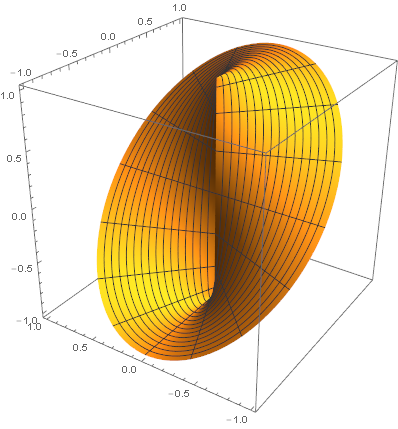
\includegraphics[height=0.3\textheight]{Figures16/COSTHETA-1.png} }}
%	\subfloat[]{\label{costheta-2}
%{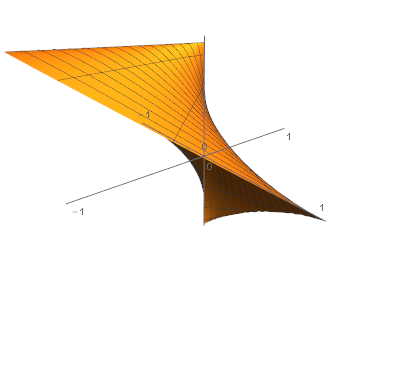
\includegraphics[height=0.3\textheight]{Figures16/COSTHETA-2.png} }}
%\end{center}
%\caption{函数$f(r\cos\theta,r\sin\theta)=\cos\theta,(r,\theta)\in\Set{(r,\theta)}{0<r\leqslant1,0\leqslant\theta\leqslant2\pi}$的图形}
%\label{costheta}
%\end{figure}

\begin{figure}[H]
\begin{center}
\subfigure[]{\label{costheta-1}{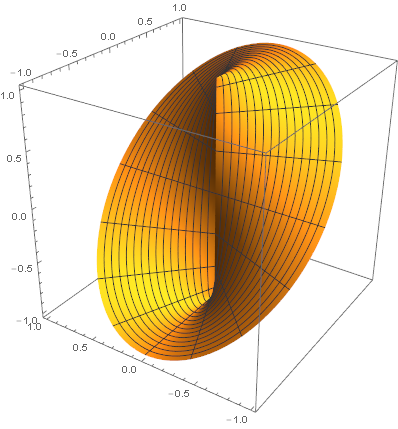
\includegraphics[height=0.3\textheight]{Figures16/COSTHETA-1.png} }}
\subfigure[]{\label{costheta-2}
{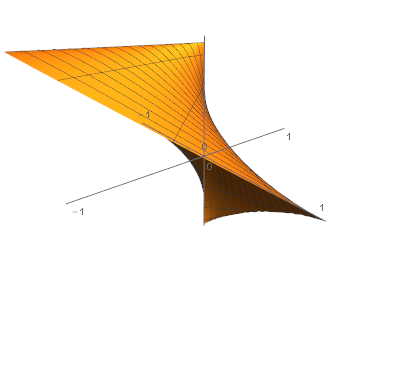
\includegraphics[height=0.3\textheight]{Figures16/COSTHETA-2.png} }}
\end{center}
\caption{函数$f(r\cos\theta,r\sin\theta)=\cos\theta,(r,\theta)\in\Set{(r,\theta)}{0<r\leqslant1,0\leqslant\theta\leqslant2\pi}$的图形}
\label{costheta}
\end{figure}

\end{enumerate}
\subsection{习题11.1解答}
\begin{enumerate}
\item设$\bm u(t),\bm v(t)$是可导的向量值函数,$\lambda(t)$为可导数值函数,求证:\\
(1)$\frac{\mathrm d}{\mathrm dt}(\lambda(t)\bm u(t))=\frac{\mathrm d\lambda(t)}{\mathrm dt}\bm u(t)+\lambda(t)\frac{\mathrm d}{\mathrm dt}\bm u(t)$;\\
(2)$\frac{\mathrm d}{\mathrm dt}(\bm u(t)\bm\cdot\bm v(t))=(\frac{\mathrm d}{\mathrm dt}\bm u(t))\bm\cdot\bm v(t)+\bm u(t)\bm\cdot(\frac{\mathrm d}{\mathrm dt}\bm v(t))$.

证明:(1)设$\bm u(t)=(u_1(t),u_2(t),u_3(t))$,则$\lambda(t)\bm u(t)=(\lambda(t)u_1(t),\lambda(t)u_2(t),\lambda(t)u_3(t))$,
\[\begin{split}
\frac{\mathrm d}{\mathrm dt}(\lambda(t)\bm u(t))&=({\mathrm dt}[\lambda(t)u_1(t)]',[\lambda(t)u_2(t)]',[\lambda(t)u_3(t)]')\\
&=(\lambda'(t)u_1(t)+\lambda(t)u'_1(t),\lambda'(t)u_2(t)+\lambda(t)u'_2(t),\lambda'(t)u_3(t)+\lambda(t)u'_3(t))\\
&=(\lambda'(t)u_1(t),\lambda'(t)u_2(t),\lambda'(t)u_3(t))+(\lambda(t)u'_1(t),\lambda(t)u'_2(t),\lambda(t)u'_3(t))\\
&=\lambda'(t)(u_1(t),u_2(t),u_3(t))+\lambda(t)(u'_1(t),u'_2(t),u'_3(t))\\
&=\frac{\mathrm d\lambda(t)}{\mathrm dt}\bm u(t)+\lambda(t)\frac{\mathrm d}{\mathrm dt}\bm u(t).
\end{split}\]
(2)设$\bm u(t)=(u_1(t),u_2(t),u_3(t)),\bm v(t)=(v_1(t),v_2(t),v_3(t))$,

则$\bm u(t)\bm\cdot\bm v(t)=u_1(t)v_1(t)+u_2(t)v_2(t)+u_3(t)v_3(t)$,
\[\begin{split}
\frac{\mathrm d}{\mathrm dt}(\bm u(t)\bm\cdot\bm v(t))&=\frac{\mathrm d}{\mathrm dt}[u_1(t)v_1(t)+u_2(t)v_2(t)+u_3(t)v_3(t)]\\
&=u'_1(t)v_1(t)+u_1(t)v'_1(t)+u'_2(t)v_2(t)+u_2(t)v'_2(t)+u'_3(t)v_3(t)+u_3(t)v'_3(t)\\
&=u'_1(t)v_1(t)+u'_2(t)v_2(t)+u'_3(t)v_3(t)+u_1(t)v'_1(t)+u_2(t)v'_2(t)+u_3(t)v'_3(t)\\
&=(\frac{\mathrm d}{\mathrm dt}\bm u(t))\bm\cdot\bm v(t)+\bm u(t)\bm\cdot(\frac{\mathrm d}{\mathrm dt}\bm v(t)).
\end{split}\]
\item求下列曲线在指定点的单位切向量:\\
(1)$\bm r(t)=(\mathrm e^{2t},\mathrm e^{-2t},t\mathrm e^{2t}),t=0$;\\
(2)$\bm r(t)=t\bm i+2\sin t\bm j+3\cos t\bm k,t=\frac\pi6$.

解:(1)单位切向量$\bm t=\frac{\bm r'(t)}{|\bm r'(t)|}=\frac{(2\mathrm e^{2t},-2\mathrm e^{-2t},(1+2t)\mathrm e^{2t})}{\|(2\mathrm e^{2t},-2\mathrm e^{-2t},(1+2t)\mathrm e^{2t})\|}\Big|_{t=0}=\frac{(2,-2,1)}{\sqrt{4+4+1}}=(\frac23,-\frac23,\frac13)$.

(2)单位切向量$\bm t=\frac{\bm r'(t)}{|\bm r'(t)|}=\frac{\bm i+2\cos t\bm j-3\sin t\bm k}{\|\bm i+2\cos t\bm j-3\sin t\bm k\|}\Big|_{t=\frac\pi6}=\frac{\bm i+\sqrt3\bm j-\frac32\bm k}{\sqrt{1+3+\frac94}}=\frac25\bm i+\frac{2\sqrt3}5\bm j-\frac35\bm k$.

\item求下列曲线在指定点的切线方程:\\
(1)$\bm r(t)=(1+2t,1+t-t^2,1-t+t^2-t^3),M(1,1,1)$;\\
(2)$\bm r(t)=\sin(\pi t)\bm i+\sqrt t\bm j+\cos(\pi t)\bm k,M(0,1,-1)$.

解:(1)在$M(1,1,1)$点处$t=0$,切向量$\bm t=\bm r'(0)=(2,1-2t,-1+2t-3t^2)_{t=0}=(2,1,-1)$,则切线方程为
\[\frac{x-1}2=y-1=-(z-1).\]
(2)在$M(0,1,-1)$点处$t=1$,切向量$\bm t=\bm r'(1)=\pi\cos(\pi t)\bm i+\frac1{2\sqrt t}\bm j-\pi\sin(\pi t)\bm k\big|_{t=1}=-\pi\bm i+\frac12\bm j$,则切线方程为$\begin{cases}
\frac x{-\pi}=2(y-1),\\
z=-1,
\end{cases}$即$\begin{cases}
x+2\pi y=2\pi,\\
z=-1.
\end{cases}$

\item求下列向量值函数的积分:\\
(1)$\int_0^{\frac\pi4}[\cos(2t)\bm i+\sin(2t)\bm j+t\sin t\bm k]\mathrm dt$;\\
(2)$\int_1^4(\sqrt t\bm i+t\mathrm e^{-t}\bm j+\frac1{t^2}\bm k)\mathrm dt$.

解:(1)$\int_0^{\frac\pi4}[\cos(2t)\bm i+\sin(2t)\bm j+t\sin t\bm k]\mathrm dt=\int_0^{\frac\pi4}\cos(2t)\mathrm dt\bm i+\int_0^{\frac\pi4}\sin(2t)\mathrm dt\bm j+\int_0^{\frac\pi4}t\sin t\mathrm dt\bm k$,

$\because\int_0^{\frac\pi4}\cos(2t)\mathrm dt=\frac12\sin(2t)\big|_0^{\frac\pi4}=\frac12,\ \int_0^{\frac\pi4}\sin(2t)\mathrm dt=-\frac12\cos(2t)\big|_0^{\frac\pi4}=\frac12,\\
\int_0^{\frac\pi4}t\sin t\mathrm dt=-\int_0^{\frac\pi4}t\mathrm d\cos t=-t\cos t\big|_0^{\frac\pi4}+\int_0^{\frac\pi4}\cos t\mathrm dt=-\frac{\sqrt2\pi}{8}+\sin t\big|_0^{\frac\pi4}=-\frac{\sqrt2\pi}{8}+\frac{\sqrt2}2$,

$\therefore\int_0^{\frac\pi4}[\cos(2t)\bm i+\sin(2t)\bm j+t\sin t\bm k]\mathrm dt=\frac12\bm i+\frac12\bm j+(-\frac{\sqrt2\pi}{8}+\frac{\sqrt2}2)\bm k$.

(2)$\int_1^4(\sqrt t\bm i+t\mathrm e^{-t}\bm j+\frac1{t^2}\bm k)\mathrm dt=\int_1^4\sqrt t\mathrm dt\bm i+\int_1^4t\mathrm e^{-t}\mathrm dt\bm j+\int_1^4\frac1{t^2}\mathrm dt\bm k$,

$\because\int_1^4\sqrt t\mathrm dt=\frac1{1+\frac12}t^{\frac12+1}\big|_1^4=\frac{14}3,\int_1^4t\mathrm e^{-t}\mathrm dt=-\int_1^4t\mathrm d\mathrm e^{-t}=-t\mathrm e^{-t}\big|_1^4+\int_1^4\mathrm e^{-t}\mathrm dt\\
=-4\mathrm e^{-4}+\mathrm e^{-1}-\mathrm e^{-t}\big|_1^4=-4\mathrm e^{-4}+\mathrm e^{-1}-\mathrm e^{-4}+\mathrm e^{-1}=-5\mathrm e^{-4}+2\mathrm e^{-1},\\
\int_1^4\frac1{t^2}\mathrm dt=\frac1{-2+1}t^{-2+1}\big|_1^4=-\frac14+1=\frac34$,

$\therefore\int_1^4(\sqrt t\bm i+t\mathrm e^{-t}\bm j+\frac1{t^2}\bm k)\mathrm dt=\frac{14}3\bm i+(-5\mathrm e^{-4}+2\mathrm e^{-1})\bm j+\frac34\bm k$.

\item已知$\bm r'(t),\bm r(0)$,求$\bm r(t)$:\\
(1)$\bm r'(t)=(t^2,4t^3,-t^2),\bm r(0)=(0,1,0)$;\\
(2)$\bm r'(t)=\sin t\bm i-\cos t\bm j+2t\bm k,\bm r(0)=\bm i+\bm j+2\bm k$.

解:(1)方法1:
\[\begin{split}
\bm r(t)&=\int_0^t\bm r'(t)\mathrm dt+\bm C=(\int_0^tt^2\mathrm dt+C_1,\int_0^t4t^3\mathrm dt+C_2,\int_0^t(-t^2)\mathrm dt+C_3)\\
&=(\frac13t^3+C_1,t^4+C_2,-\frac13t^3+C_3),
\end{split}\]
$\therefore\bm r(0)=(C_1,C_2,C_3)=(0,1,0)$,

$\therefore\bm r(t)=(\frac13t^3,t^4+1,-\frac13t^3)$.

方法2:$\because\int t^2\mathrm dt=\frac13t^3+C,\ \int4t^3\mathrm dt=t^4+C,\ \int(-t^2)\mathrm dt=-\frac13t^3+C$,

$\therefore r(t)=\int\bm r'(t)\mathrm dt=(\frac13t^3+C_1,t^4+C_2,-\frac13t^3+C_3)$,

$\because\bm r(0)=(0,1,0)$,

$\therefore C_1=0,\ C_2=1,\ C_3=0$,

$\therefore\bm r(t)=(\frac13t^3,t^4+1,-\frac13t^3)$.

(2)方法1:\[\begin{split}
\bm r(t)=&\int_0^t\bm r'(t)\mathrm dt+\bm C=(\int_0^t\sin t\mathrm dt+C_1)\bm i+(-\int_0^t\cos t\mathrm dt+C_2)\bm j+(\int_0^t2t\mathrm dt+C_3)\bm k\\
=&(-\cos t+C_1)\bm i+(-\sin t+C_2)\bm j+(t^2+C_3)\bm k,
\end{split}\]
$\because\bm r(0)=(-1+C_1)\bm i+C_2\bm j+C_3\bm k=\bm i+\bm j+2\bm k$,

$\therefore C_1=2,C_2=1,C_3=2$,

$\therefore\bm r(t)=(-\cos t+2)\bm i+(-\sin t+1)\bm j+(t^3+2)\bm k$.

方法2:$\because\int\sin t\mathrm dt=-\cos t+C,\ \int(-\cos t)\mathrm dt=-\sin t+C,\ \int2t\mathrm dt=t^2+C$,

$\therefore\bm r(t)=\int\bm r'(t)\mathrm dt=(-\cos t+C_1)\bm i+(-\sin t+C_2)\bm j+(t^2+C_3)\bm k$,

$\because\bm r(0)=\bm i+\bm j+2\bm k$,

$\therefore C_1=2,\ C_2=1,\ C_3=2$,

$\therefore\bm r(t)=(-\cos t+2)\bm i+(-\sin t+1)\bm j+(t^3+2)\bm k$.

\item证明下列等式:\\
(1)$\frac{\mathrm d}{\mathrm dt}(\bm r(t)\times\bm r'(t))=\bm r(t)\times\bm r''(t)$;\\
(2)$\frac{\mathrm d}{\mathrm dt}\|\bm r(t)\|=\frac{\bm r(t)\bm\cdot\bm r'(t)}{\|\bm r(t)\|}(\bm r(t)\neq\bm0)$;\\
(3)$\frac{\mathrm d}{\mathrm dt}[\bm r(t)\bm\cdot(\bm r'(t)\times\bm r''(t))]=\bm r(t)\bm\cdot[\bm r'(t)\times\bm r'''(t)]$.

证明:(1)$\frac{\mathrm d}{\mathrm dt}(\bm r(t)\times\bm r'(t))=\bm r'(t)\times\bm r'(t)+\bm r(t)\times\bm r''(t)=\bm r(t)\times\bm r''(t)$.

(2)$\frac{\mathrm d}{\mathrm dt}\|\bm r(t)\|=\frac{\mathrm d}{\mathrm dt}\sqrt{\bm r(t)\bm\cdot\bm r(t)}=\frac1{2\sqrt{\bm r(t)\bm\cdot\bm r(t)}}\frac{\mathrm d}{\mathrm dt}[\bm r(t)\bm\cdot\bm r(t)]\\
=\frac1{2\sqrt{\bm r(t)\bm\cdot\bm r(t)}}[\bm r'(t)\bm\cdot\bm r(t)+\bm r(t)\bm\cdot\bm r'(t)]=\frac{2\bm r(t)\bm\cdot\bm r'(t)}{2\sqrt{\bm r(t)\bm\cdot\bm r(t)}}=\frac{\bm r(t)\bm\cdot\bm r'(t)}{\|\bm r(t)\|}(\bm r(t)\neq\bm0)$.

(3)$\frac{\mathrm d}{\mathrm dt}[\bm r(t)\bm\cdot(\bm r'(t)\times\bm r''(t))]=\bm r'(t)\bm\cdot(\bm r'(t)\times\bm r''(t))+\bm r(t)\bm\cdot\frac{\mathrm d}{\mathrm dt}(\bm r'(t)\times\bm r''(t))\\
=\bm r(t)\bm\cdot\frac{\mathrm d}{\mathrm dt}(\bm r'(t)\times\bm r''(t))=\bm r(t)\bm\cdot(\bm r''(t)\times\bm r''(t)+\bm r'(t)\times\bm r'''(t))=\bm r(t)\bm\cdot[\bm r'(t)\times\bm r'''(t)]$.

\item求等速圆周运动$\bm r=R\cos(\omega t)\bm i+R\sin(\omega t)\bm j$在$t$时刻的速度与加速度.

解:$t$时刻的速度$\bm v(t)=\bm r'(t)=-R\omega\sin(\omega t)\bm i+R\omega\cos(\omega t)\bm j$,

$t$时刻的加速度$\bm a(t)=\bm v'(t)=-R\omega^2\cos(\omega t)\bm i-R\omega^2\sin(\omega t)\bm j$.

\item已知螺旋线的向量方程为$\bm r=a\cos\theta\bm i+a\sin\theta\bm j+b\theta\bm k(a>0,b>0)$,求在$\theta_0$处的切线方程.

解:在$\theta_0$处的切向量$\bm r'(\theta_0)=-a\sin\theta_0\bm i+a\cos\theta_0\bm j+b\bm k$,切线方程
\[\frac{x-a\cos\theta_0}{-a\sin\theta_0}=\frac{y-a\sin\theta_0}{a\cos\theta_0}=\frac{z-b\theta_0}b.\]

\item设$\bm r=-a\sin\theta\bm i+a\cos\theta\bm j+b\theta\bm k$,求$\frac12\int_0^{2\pi}(\bm r\times\bm r')\mathrm d\theta$.

解:$\bm r'(\theta)=-a\cos\theta\bm i-a\sin\theta\bm j+b\bm k$,

$\bm r(\theta)\times\bm r'(\theta)=\begin{vmatrix}
\bm i&\bm j&\bm k\\
-a\sin\theta&a\cos\theta&b\theta\\
-a\cos\theta&-a\sin\theta&b
\end{vmatrix}=\begin{vmatrix}
a\cos\theta&b\theta\\
-a\sin\theta&b
\end{vmatrix}\bm i+\begin{vmatrix}
b\theta&-a\sin\theta\\
b&-a\cos\theta
\end{vmatrix}\bm j+\begin{vmatrix}
-a\sin\theta&a\cos\theta\\
-a\cos\theta&-a\sin\theta
\end{vmatrix}\bm k\\
=(ab\cos\theta+ab\theta\sin\theta)\bm i-(-ab\sin\theta+ab\theta\cos\theta)\bm j+a^2\bm k$,

$\because\int_0^{2\pi}(ab\cos\theta+ab\theta\sin\theta)\mathrm d\theta=ab\sin\theta\big|_0^{2\pi}-\int_0^{2\pi}ab\theta\mathrm d\cos\theta\\
=-ab\theta\cos\theta\big|_0^{2\pi}+\int_0^{2\pi}ab\cos\theta\mathrm d\theta=-2\pi ab+ab\sin\theta\big|_0^{2\pi}=-2\pi ab,\\
\int_0^{2\pi}-(-ab\sin\theta+ab\theta\cos\theta)\mathrm d\theta=\int_0^{2\pi}(ab\sin\theta-ab\theta\cos\theta)\mathrm d\theta=-ab\cos\theta\big|_0^{2\pi}-ab\int_0^{2\pi}\theta\mathrm d\sin\theta\\
=-ab\theta\sin\theta\big|_0^{2\pi}+ab\int_0^{2\pi}\sin\theta\mathrm d\theta=-ab\cos\theta\big|_0^{2\pi}=0,\\
\int_0^{2\pi}a^2\mathrm d\theta=2\pi a^2$,

$\therefore\frac12\int_0^{2\pi}(\bm r\times\bm r')\mathrm d\theta=-\pi ab\bm i+\pi a^2\bm k$.
\end{enumerate}
\subsection{习题11.2解答}
\begin{enumerate}
\item求下列曲面在指定点的法线方程与切平面的方程:\\
(1)$x^2+y^2+z^2=14$,在点$(1,2,3)$;\\
(2)$z=\frac12x^2-y^2$,在点$(2,-1,1)$;\\
(3)$(2a^2-z^2)x^2-a^2y^2=0$,在点$(a,a,a)$;\\
(4)$\frac{x^2}{a^2}+\frac{y^2}{b^2}+\frac{z^2}{c^2}=1$,在点$(\frac a{\sqrt3},\frac b{\sqrt3},\frac c{\sqrt3})$;\\
(5)$\begin{cases}
x=u\cos v,\\
y=u\sin v,\\
z=av,
\end{cases}$在$(u,v)=(u_0,v_0)$处.

解:(1)法向量$\bm n=(2x,2y,2z)\big|_{(1,2,3)}=2(1,2,3)$,

法线方程$x-1=\frac{y-2}2=\frac{z-3}3$,

切平面方程$(x-1)+2(y-2)+3(z-3)=0$,即$x+2y+3z=14$.

(2)法向量$\bm n=(x,-2y,-1)\big|_{(2,-1,1)}=(2,2,-1)$,

法线方程$\frac{x-2}2=\frac{y+1}2=-(z-1)$,

切平面方程$2(x-2)+2(y+1)-(z-1)=0$,即$2x+2y-z=1$.

(3)法向量$\bm n=(2(2a^2-z^2)x,-2a^2y,-2x^2z)\big|_{(a,a,a)}=2a^3(1,-1,-1)$,

法线方程$x-a=-(y-a)=-(z-a)$,

切平面方程$(x-a)-(y-a)-(z-a)=0$,即$x-y-z=-a$.

(4)法向量$\bm n=(\frac{2x}{a^2},\frac{2y}{b^2},\frac{2z}{c^2})\big|_{(\frac a{\sqrt3},\frac b{\sqrt3},\frac c{\sqrt3})}=\frac2{\sqrt3}(\frac1a,\frac1b,\frac1c)$,

法线方程$a(x-\frac a{\sqrt3})=b(y-\frac b{\sqrt3})=c(z-\frac c{\sqrt3})$,

切平面方程$\frac1a(x-\frac a{\sqrt3})+\frac1b(y-\frac b{\sqrt3})+\frac1c(z-\frac c{\sqrt3})=0$,即$\frac xa+\frac yb+\frac zc=\sqrt3$.

(5)法向量$\bm n=(\cos v,\sin v,0)\times(-u\sin v,u\cos v,a)\big|_{(u_0,v_0)}=\begin{vmatrix}
\bm i&\bm j&\bm k\\
\cos v_0&\sin v_0&0\\
-u_0\sin v_0&u_0\cos v_0&a
\end{vmatrix}\\
=(\begin{vmatrix}
\sin v_0&0\\
u_0\cos v_0&a
\end{vmatrix},\begin{vmatrix}
0&a\\
a&u_0\cos v_0
\end{vmatrix},\begin{vmatrix}
\cos v_0&\sin v_0\\
-u_0\sin v_0&u_0\cos v_0
\end{vmatrix})=(a\sin v_0,-a\cos v_0,u_0)$,

法线方程$\frac{x-u_0\cos v_0}{a\sin v_0}=\frac{y-u_0\sin v_0}{-a\cos v_0}=\frac{z-av_0}{u_0}$,

切平面方程$a\sin v_0(x-u_0\cos v_0)-a\cos v_0(y-u_0\sin v_0)+u_0(z-av_0)=0$,\\
即$ax\sin v_0-ay\cos v_0+zu_0=au_0v_0$.

\item按要求求下列曲面的切平面方程:\\
(1)曲面$x^2+2y^2+3z^2=21$的与平面$x+4y+6z=0$平行的切平面;\\
(2)曲面$z=x^2+y^2$的与直线$\begin{cases}
x+2z=1,\\
y+2z=2
\end{cases}$垂直的切平面;\\
(3)双曲抛物面$\bm r=(u+v,u-v,uv)$在$u=1,v=-1$处的切平面.

解:(1)曲面的法向量$\bm n=(2x,4y,6z)$,平面的法向量$\bm n_1=(1,4,6)$,\\则由$\begin{cases}(2x,4y,6z)=a(1,4,6),\\
x^2+2y^2+3z^2=21
\end{cases}$得曲面上与该平面相切的切平面的切点为$\pm(1,2,2)$,

切平面方程$x-1+4(y-2)+6(z-2)=0$或$x+1+4(y+2)+6(z+2)=0$,即$x+4y+6z=\pm21$.

(2)直线的切向量$\bm t=(1,0,2)\times(0,1,2)=\begin{vmatrix}
\bm i&\bm j&\bm k\\
1&0&2\\
0&1&2\\
\end{vmatrix}=(\begin{vmatrix}
0&2\\
1&2
\end{vmatrix},\begin{vmatrix}
2&1\\
2&0
\end{vmatrix},\begin{vmatrix}
1&0\\
0&1
\end{vmatrix})=(-2,-2,1)$,曲面的法向量$\bm n=(2x,2y,-1)$,曲面上与直线垂直的切平面的法向量$\bm n_0=a\bm t$,\\
由$\begin{cases}
(2x,2y,-1)=a(-2,-2,1),\\
z=x^2+y^2
\end{cases}$可得切点为$(1,1,2)$,

切平面方程$-2(x-1)-2(y-1)+z-2=0$,即$2x+2y-z=2$.

(3)法向量$\bm n=(1,1,v)\times(1,-1,u)\big|_{(1,-1)}=\begin{vmatrix}
\bm i&\bm j&\bm k\\
1&1&-1\\
1&-1&1
\end{vmatrix}=(\begin{vmatrix}
1&-1\\
-1&1
\end{vmatrix},\begin{vmatrix}
-1&1\\
1&1
\end{vmatrix},\begin{vmatrix}
1&1\\
1&-1
\end{vmatrix})\\
=(0,-2,-2)$,切点为$(0,2,-1)$,

切平面的方程$-2(y-2)-2(z+1)=0$,即$y+z=1$.

\item求证:曲面$\sqrt x+\sqrt y+\sqrt z=\sqrt a,a>0$在任意点处的切平面在各坐标轴上的截距之和为$a$.

证明:曲面在任意点$(x_0,y_0,z_0)$处的法向量$\bm n=\frac12(\frac1{\sqrt{x_0}},\frac1{\sqrt{y_0}},\frac1{\sqrt{z_0}})$,\\
切平面方程$\frac1{\sqrt{x_0}}(x-x_0)+\frac1{\sqrt{y_0}}(y-y_0)+\frac1{\sqrt{z_0}}(z-z_0)=0$,即$\frac x{ax_0}+\frac y{ay_0}+\frac z{az_0}=1$,

切平面在$x,y,z$轴上的截距之和
\[\begin{split}
\sqrt{ax_0}+\sqrt{ay_0}+\sqrt{az_0}=\sqrt a(\sqrt{x_0}+\sqrt{y_0}+\sqrt{z_0})=a.
\end{split}\]

\item证明二次曲面$ax^2+by^2+cz^2=1$在点$M_0(x_0,y_0,z_0)$处的切平面方程为
\[
ax_0x+by_0y+cz_0z=1.
\]
证明:曲面在点$M_0(x_0,y_0,z_0)$处的法向量$\bm n=2(ax_0,by_0,cz_0)$,

切平面方程
\[\begin{split}
&ax_0(x-x_0)+by_0(y-y_0)+cz_0(z-z_0)\\
=&ax_0x-ax_0^2+by_0y-by_0^2+cz_0z-cz_0^2\\
=&ax_0x-by_0y-cz_0z-1=0,
\end{split}\]
即\[
ax_0x+by_0y+cz_0z=1.
\]

\item设函数$f$可微,试证曲面$z=yf(\frac xy)$的所有切平面相交于一个公共点.

证明:曲面在点$(x_0,y_0,z_0)$处的法向量$\bm n=(yf'(\frac xy)\frac1y,f(\frac xy)+yf'(\frac xy)(-\frac x{y^2}),-1)\big|_{(x_0,y_0,z_0)}\\
=(f'(\frac{x_0}{y_0}),f(\frac{x_0}{y_0})-\frac{x_0}{y_0}f'(\frac{x_0}{y_0}),-1)$,

切平面的方程
\[\begin{split}
&f'(\frac{x_0}{y_0})(x-x_0)+[f(\frac{x_0}{y_0})-\frac{x_0}{y_0}f'(\frac{x_0}{y_0})](y-y_0)-(z-z_0)\\
=&f'(\frac{x_0}{y_0})x+[f(\frac{x_0}{y_0})-\frac{x_0}{y_0}f'(\frac{x_0}{y_0})]y-z-x_0f'(\frac{x_0}{y_0})-y_0f(\frac{x_0}{y_0})+x_0f'(\frac{x_0}{y_0})+z_0\\
=&f'(\frac{x_0}{y_0})x+[f(\frac{x_0}{y_0})-\frac{x_0}{y_0}f'(\frac{x_0}{y_0})]y-z\\
%=&f'(\frac{x_0}{y_0})(x-\frac{x_0}{y_0}y)+f(\frac{x_0}{y_0})y-z\\
%=&f'(\frac{x_0}{y_0})(x-\frac{x_0}{y_0}y)+\frac{z_0}{y_0}y-z\\
=&0,
\end{split}\]
$\because$无论切点$(x_0,y_0,z_0)$取在何处,点$(x,y,z)=(0,0,0)$始终满足以上方程,

$\therefore$曲面$z=yf(\frac xy)$的所有切平面相交于一个公共点$(0,0,0)$.

\item已知函数$f$可微,证明曲面$f(\frac{x-a}{z-c},\frac{y-b}{z-c})=0$上任意一点处的切平面通过一定点,并求出此点的位置.

证明:曲面上任一点$(x_0,y_0,z_0)$处的法向量
\[
\bm n=(\frac1{z_0-c}f'_1,\frac1{z_0-c}f'_2,-\frac{x_0-a}{(z_0-c)^2}f'_1-\frac{y_0-b}{(z_0-c)^2}f'_2),
\]
切平面方程
\[\begin{split}
&\frac{x-x_0}{z_0-c}f'_1+\frac{y-y_0}{z_0-c}f'_2+[-\frac{x_0-a}{(z_0-c)^2}f'_1-\frac{y_0-b}{(z_0-c)^2}f'_2](z-z_0)\\
=&[\frac{x-x_0}{z_0-c}-\frac{x_0-a}{(z_0-c)^2}(z-z_0)]f'_1+[\frac{y-y_0}{z_0-c}-\frac{y_0-b}{(z_0-c)^2}(z-z_0)]f'_2\\
=&0,
\end{split}\]
其中偏导数均在$(\frac{x_0-a}{z_0-c},\frac{y_0-b}{z_0-c})$处取值,

$\because$无论切点$(x_0,y_0,z_0)$取在何处,$(x,y,z)=(a,b,c)$始终满足以上方程,

$\therefore$曲面$f(\frac{x-a}{z-c},\frac{y-b}{z-c})=0$上任意一点处的切平面通过定点$(a,b,c)$.

\item设曲面$S_1$和$S_2$的方程分别为$F_1(x,y,z)=0,F_2(x,y,z)=0$,其中$F_1$和$F_2$是可微函数,试证$S_1$与$S_2$垂直的充分必要条件是对交线上的任意一点$(x,y,z)$,均有
\[
\frac{\partial F_1}{\partial x}\frac{\partial F_2}{\partial x}+\frac{\partial F_1}{\partial y}\frac{\partial F_2}{\partial y}+\frac{\partial F_1}{\partial z}\frac{\partial F_2}{\partial z}=0.
\]
证明:必要性:$\because S_1$与$S_2$垂直,

$\therefore$交线上的任意一点$(x,y,z)$处两曲面的法向量互相垂直,即
\[
(\frac{\partial F_1}{\partial x},\frac{\partial F_1}{\partial y},\frac{\partial F_1}{\partial z})\bm\cdot(\frac{\partial F_2}{\partial x},\frac{\partial F_2}{\partial y},\frac{\partial F_2}{\partial z})=\frac{\partial F_1}{\partial x}\frac{\partial F_2}{\partial x}+\frac{\partial F_1}{\partial y}\frac{\partial F_2}{\partial y}+\frac{\partial F_1}{\partial z}\frac{\partial F_2}{\partial z}=0;
\]
充分性:$\because$交线上的任意一点$(x,y,z)$处
\[
\frac{\partial F_1}{\partial x}\frac{\partial F_2}{\partial x}+\frac{\partial F_1}{\partial y}\frac{\partial F_2}{\partial y}+\frac{\partial F_1}{\partial z}\frac{\partial F_2}{\partial z}=(\frac{\partial F_1}{\partial x},\frac{\partial F_1}{\partial y},\frac{\partial F_1}{\partial z})\bm\cdot(\frac{\partial F_2}{\partial x},\frac{\partial F_2}{\partial y},\frac{\partial F_2}{\partial z})=0,
\]
$\therefore$交线上的任意一点$(x,y,z)$处曲面$S_1$与$S_2$的法向量互相垂直,

$\therefore S_1$与$S_2$垂直.

\item已知函数$F$可微,若$T$为曲面$S:\ F(x,y,z)=0$在点$M_0(x_0,y_0,z_0)$处的切平面,$l$为$T$上任意一条过$M_0$的直线,求证:在$S$上存在一条曲线,该曲线在$M_0$处的切线恰好为$l$.

证明:方法1:设直线$l$的方程为$\frac{x-x_0}a=\frac{y-y_0}b=\frac{z-z_0}c$,因$l$在$T$上,其方向向量$(a,b,c)$应满足
\[(a,b,c)\bm\cdot\mathrm{grad}F(x_0,y_0,z_0)=aF'_x+bF'_y+cF'_z=0,\]
过直线$l$且与切平面$T$垂直的平面$A$的法向量
\[\begin{split}
\bm n&=(a,b,c)\times\mathrm{grad}F(x_0,y_0,z_0)=
\begin{vmatrix}
\bm i&\bm j&\bm k\\
a&b&c\\
F'_x&F'_y&F'_z
\end{vmatrix}=(\begin{vmatrix}
b&c\\
F'_y&F'_z
\end{vmatrix},\begin{vmatrix}
c&a\\
F'_z&F'_x
\end{vmatrix},\begin{vmatrix}
a&b\\
F'_x&F'_y
\end{vmatrix})\\
&=(bF'_z-cF'_y,cF'_x-aF'_z,aF'_y-bF'_x),
\end{split}\]
曲面$S$与平面$A$的交线在点$M_0$处的切向量
\[\begin{split}
\bm t=&\mathrm{grad}F(x_0,y_0,z_0)\times\bm n=\begin{vmatrix}
\bm i&\bm j&\bm k\\
F'_x&F'_y&F'_z\\
bF'_z-cF'_y&cF'_x-aF'_z&aF'_y-bF'_x
\end{vmatrix}\\
=&(\begin{vmatrix}
F'_y&F'_z\\
cF'_x-aF'_z&aF'_y-bF'_x
\end{vmatrix},\begin{vmatrix}
F'_z&F'_x\\
aF'_y-bF'_x&bF'_z-cF'_y
\end{vmatrix},\begin{vmatrix}
F'_x&F'_y\\
bF'_z-cF'_y&cF'_x-aF'_z
\end{vmatrix})\\
=&[a(F'_y)^2-bF'_xF'_y-cF'_xF'_z+a(F'_z)^2]\bm i-[aF'_xF'_y-b(F'_x)^2-b(F'_z)^2+cF'_yF'_z]\bm j\\
&+[c(F'_x)^2-aF'_xF'_z-bF'_yF'_z+c(F'_y)^2]\bm k\\
=&[a(F'_y)^2-F'_x(bF'_y+cF'_z)+a(F'_z)^2]\bm i-[F'_y(aF'_x+cF'_z)-b(F'_x)^2-b(F'_z)^2]\bm j\\
&+[c(F'_x)^2-F'_z(aF'_x+bF'_y)+c(F'_y)^2]\bm k\\
=&[a(F'_y)^2+a(F'_x)^2+a(F'_z)^2]\bm i-[-(F'_y)^2-b(F'_x)^2-b(F'_z)^2]\bm j+[c(F'_x)^2+c(F'_z)^2+c(F'_y)^2]\bm k\\
=&[(F'_x)^2+(F'_z)^2+(F'_y)^2](a,b,c),
\end{split}\]
$\therefore\bm t\parallel(a,b,c)$,

$\therefore$曲面$S$与平面$A$的交线在点$M_0$处的切线为$l$,即在$S$上存在一条曲线,该曲线在$M_0$处的切线恰好为$l$.

方法2:设直线$l$的方程为$\frac{x-x_0}a=\frac{y-y_0}b=\frac{z-z_0}c$,因$l$在$T$上,其方向向量$(a,b,c)$应满足
\[(a,b,c)\perp\mathrm{grad}F(x_0,y_0,z_0),\]
过直线$l$且与切平面$T$垂直的平面$A$的法向量
\[\begin{split}
\bm n&=(a,b,c)\times\mathrm{grad}F(x_0,y_0,z_0),
\end{split}\]
曲面$S$与平面$A$的交线在点$M_0$处的切向量
\[\begin{split}
\bm t=&[\mathrm{grad}F(x_0,y_0,z_0)\times\bm n]\parallel(a,b,c),
\end{split}\]

$\therefore$曲面$S$与平面$A$的交线在点$M_0$处的切线为$l$,即在$S$上存在一条曲线,该曲线在$M_0$处的切线恰好为$l$.
\end{enumerate}
\end{document} 
\documentclass[12pt,UTF8,fleqn]{ctexart}
\usepackage{ctex,amsmath,amssymb,geometry,fancyhdr,bm,amsfonts,mathtools,extarrows,graphicx,url,enumerate,xcolor,float,multicol,wasysym}
\usepackage{subfigure}
\allowdisplaybreaks[4]
% 加入中文支持
\newcommand\Set[2]{\left\{#1\ \middle\vert\ #2 \right\}}
\newcommand\Lim[0]{\lim\limits_{n\rightarrow\infty}}
\newcommand\LIM[2]{\lim\limits_{#1\rightarrow#2}}
\newcommand\Ser[1]{\sum_{n=#1}^\infty}
\newcommand{\SER}[2]{\sum_{#1=#2}^\infty}
\newcommand{\Int}[4]{\varint\nolimits_{#1}^{#2}#3\mathrm d#4}
\newcommand{\aIInt}[1]{\iint\limits_{#1}}
\newcommand{\IInt}[3]{\iint\limits_{#1}#2\mathrm d#3}
\newcommand{\varIInt}[4]{\iint\limits_{#1}#2\mathrm d#3\mathrm d#4}
\newcommand{\IIInt}[3]{\iiint\limits_{#1}#2\mathrm d#3}
\newcommand{\varIIInt}[5]{\iiint\limits_{#1}#2\mathrm d#3\mathrm d#4\mathrm d#5}
\newcommand{\LInt}[3]{\varint\nolimits_{#1}#2\mathrm d#3}
\newcommand{\LOInt}[3]{\varoint\nolimits_{#1}#2\mathrm d#3}
\newcommand{\LLInt}[4]{\varint\nolimits_{#1}\nolimits^{#2}#3\mathrm d#4}
\newcommand{\BLInt}[2]{\varint\nolimits_{#1}#2}
\newcommand{\varBLInt}[3]{\varint\nolimits_{#1}\nolimits^{#2}#3}
\newcommand{\BLOInt}[2]{\varoint\nolimits_{#1}#2}
\newcommand{\SIInt}[3]{\iint\limits_{#1}#2\mathrm d#3}
\newcommand{\md}[1]{\mathrm d#1}
\newcommand{\BSIInt}[2]{\iint\limits_{#1}#2}
\newcommand{\pp}[2]{\frac{\partial #1}{\partial #2}}
\newcommand{\ppx}[1]{\frac{\partial #1}{\partial x}}
\newcommand{\ppy}[1]{\frac{\partial #1}{\partial y}}
\newcommand{\ppz}[1]{\frac{\partial #1}{\partial z}}
\newcommand{\varppx}[1]{\frac{\partial}{\partial x} #1}
\newcommand{\varppy}[1]{\frac{\partial}{\partial y} #1}
\newcommand{\varppz}[1]{\frac{\partial}{\partial z} #1}
\newcommand{\BSOIInt}[2]{\oiint\limits_{#1}#2}
\newcommand{\me}[0]{\mathrm e}
\geometry{a4paper,scale=0.80}
\pagestyle{fancy}
\rhead{常微分方程(2)}
\lhead{基础习题课期末复习}
\chead{微积分B(2)}
\begin{document}
\setcounter{section}{16}
\section{高阶线性微分方程解的结构}
\subsection{复习计划}
\begin{figure}[H]
\begin{center}
\includegraphics[height=0.5\textheight]{Figures20190615/plan.png}
\end{center}
\end{figure}
\subsection{知识结构}
\begin{figure}[H]
\begin{center}
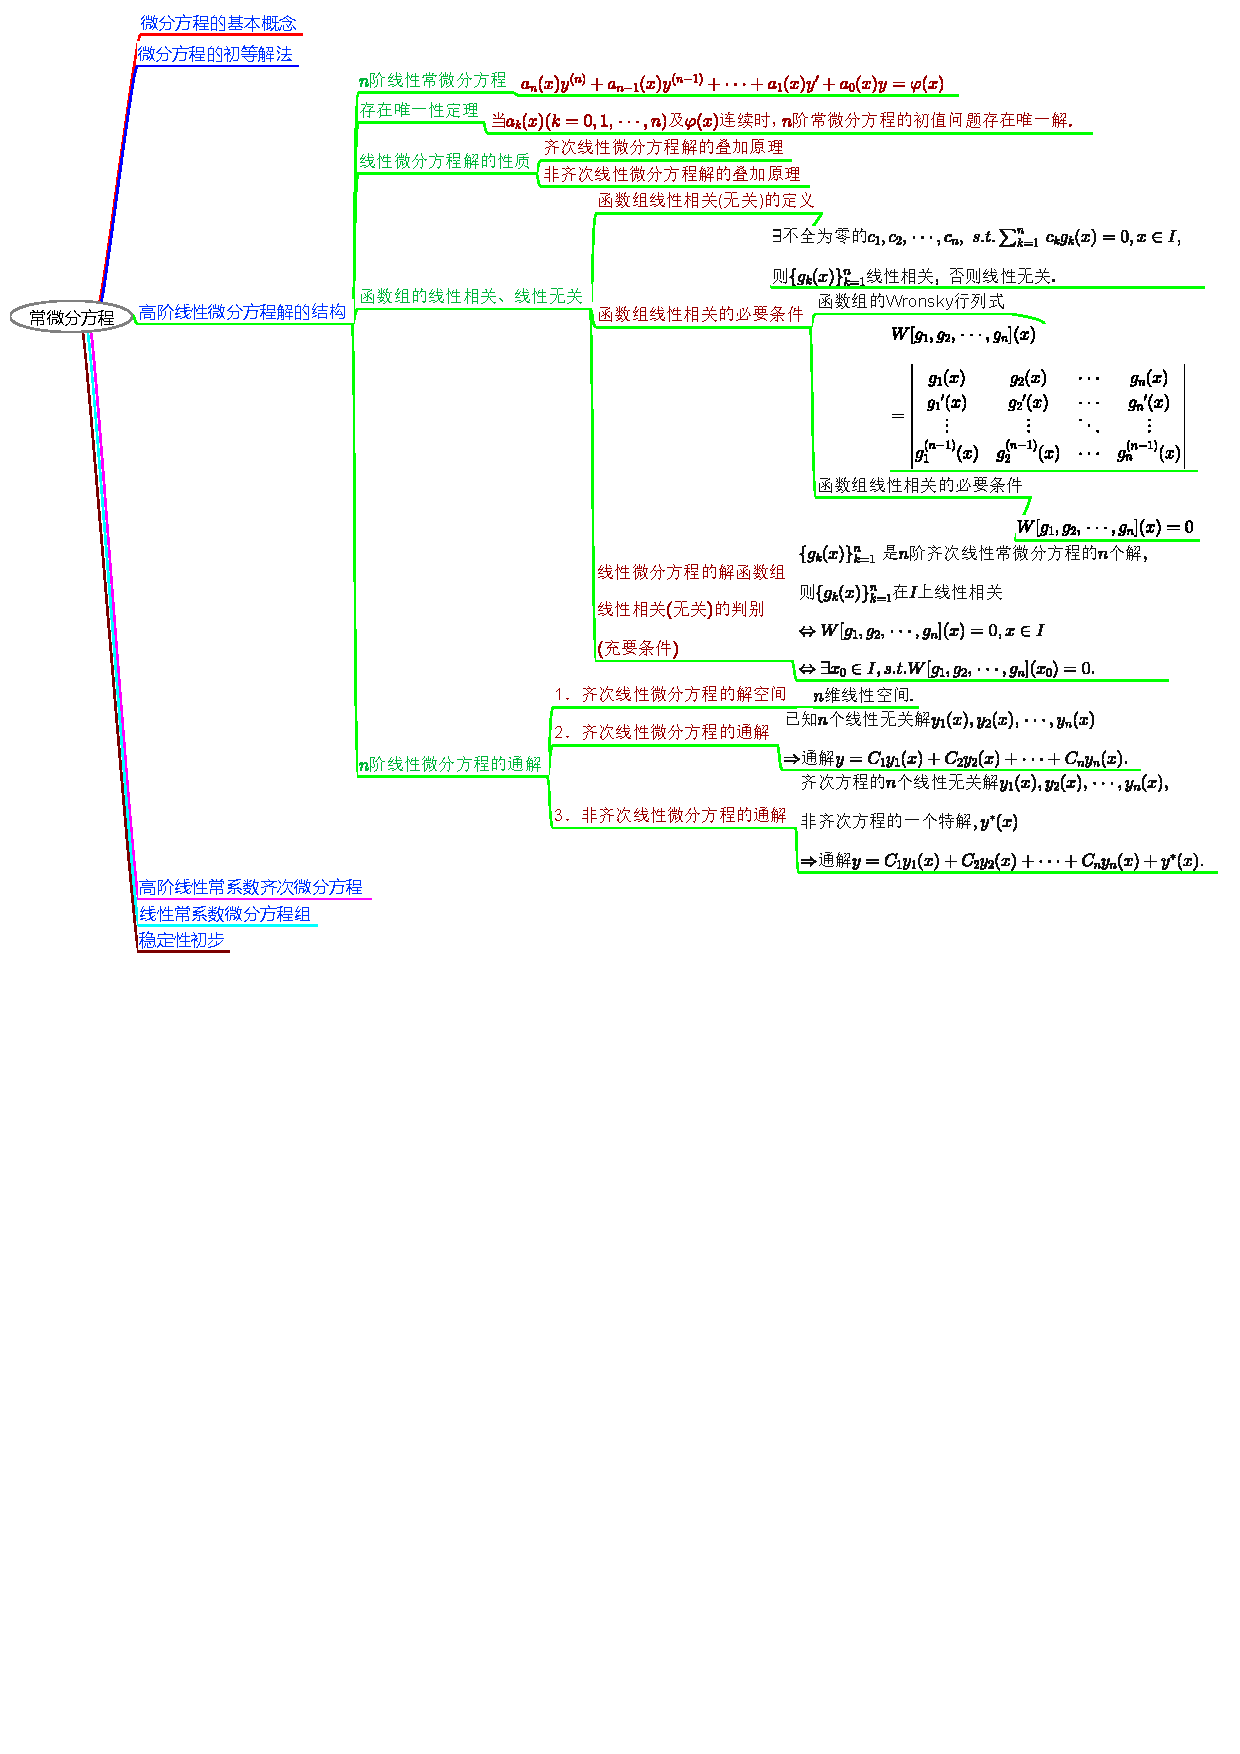
\includegraphics[height=1\textheight]{20190615-1.pdf}
\end{center}
\end{figure}
%\subsection{高阶线性微分方程解的结构}
%\begin{figure}[H]
%\begin{center}
%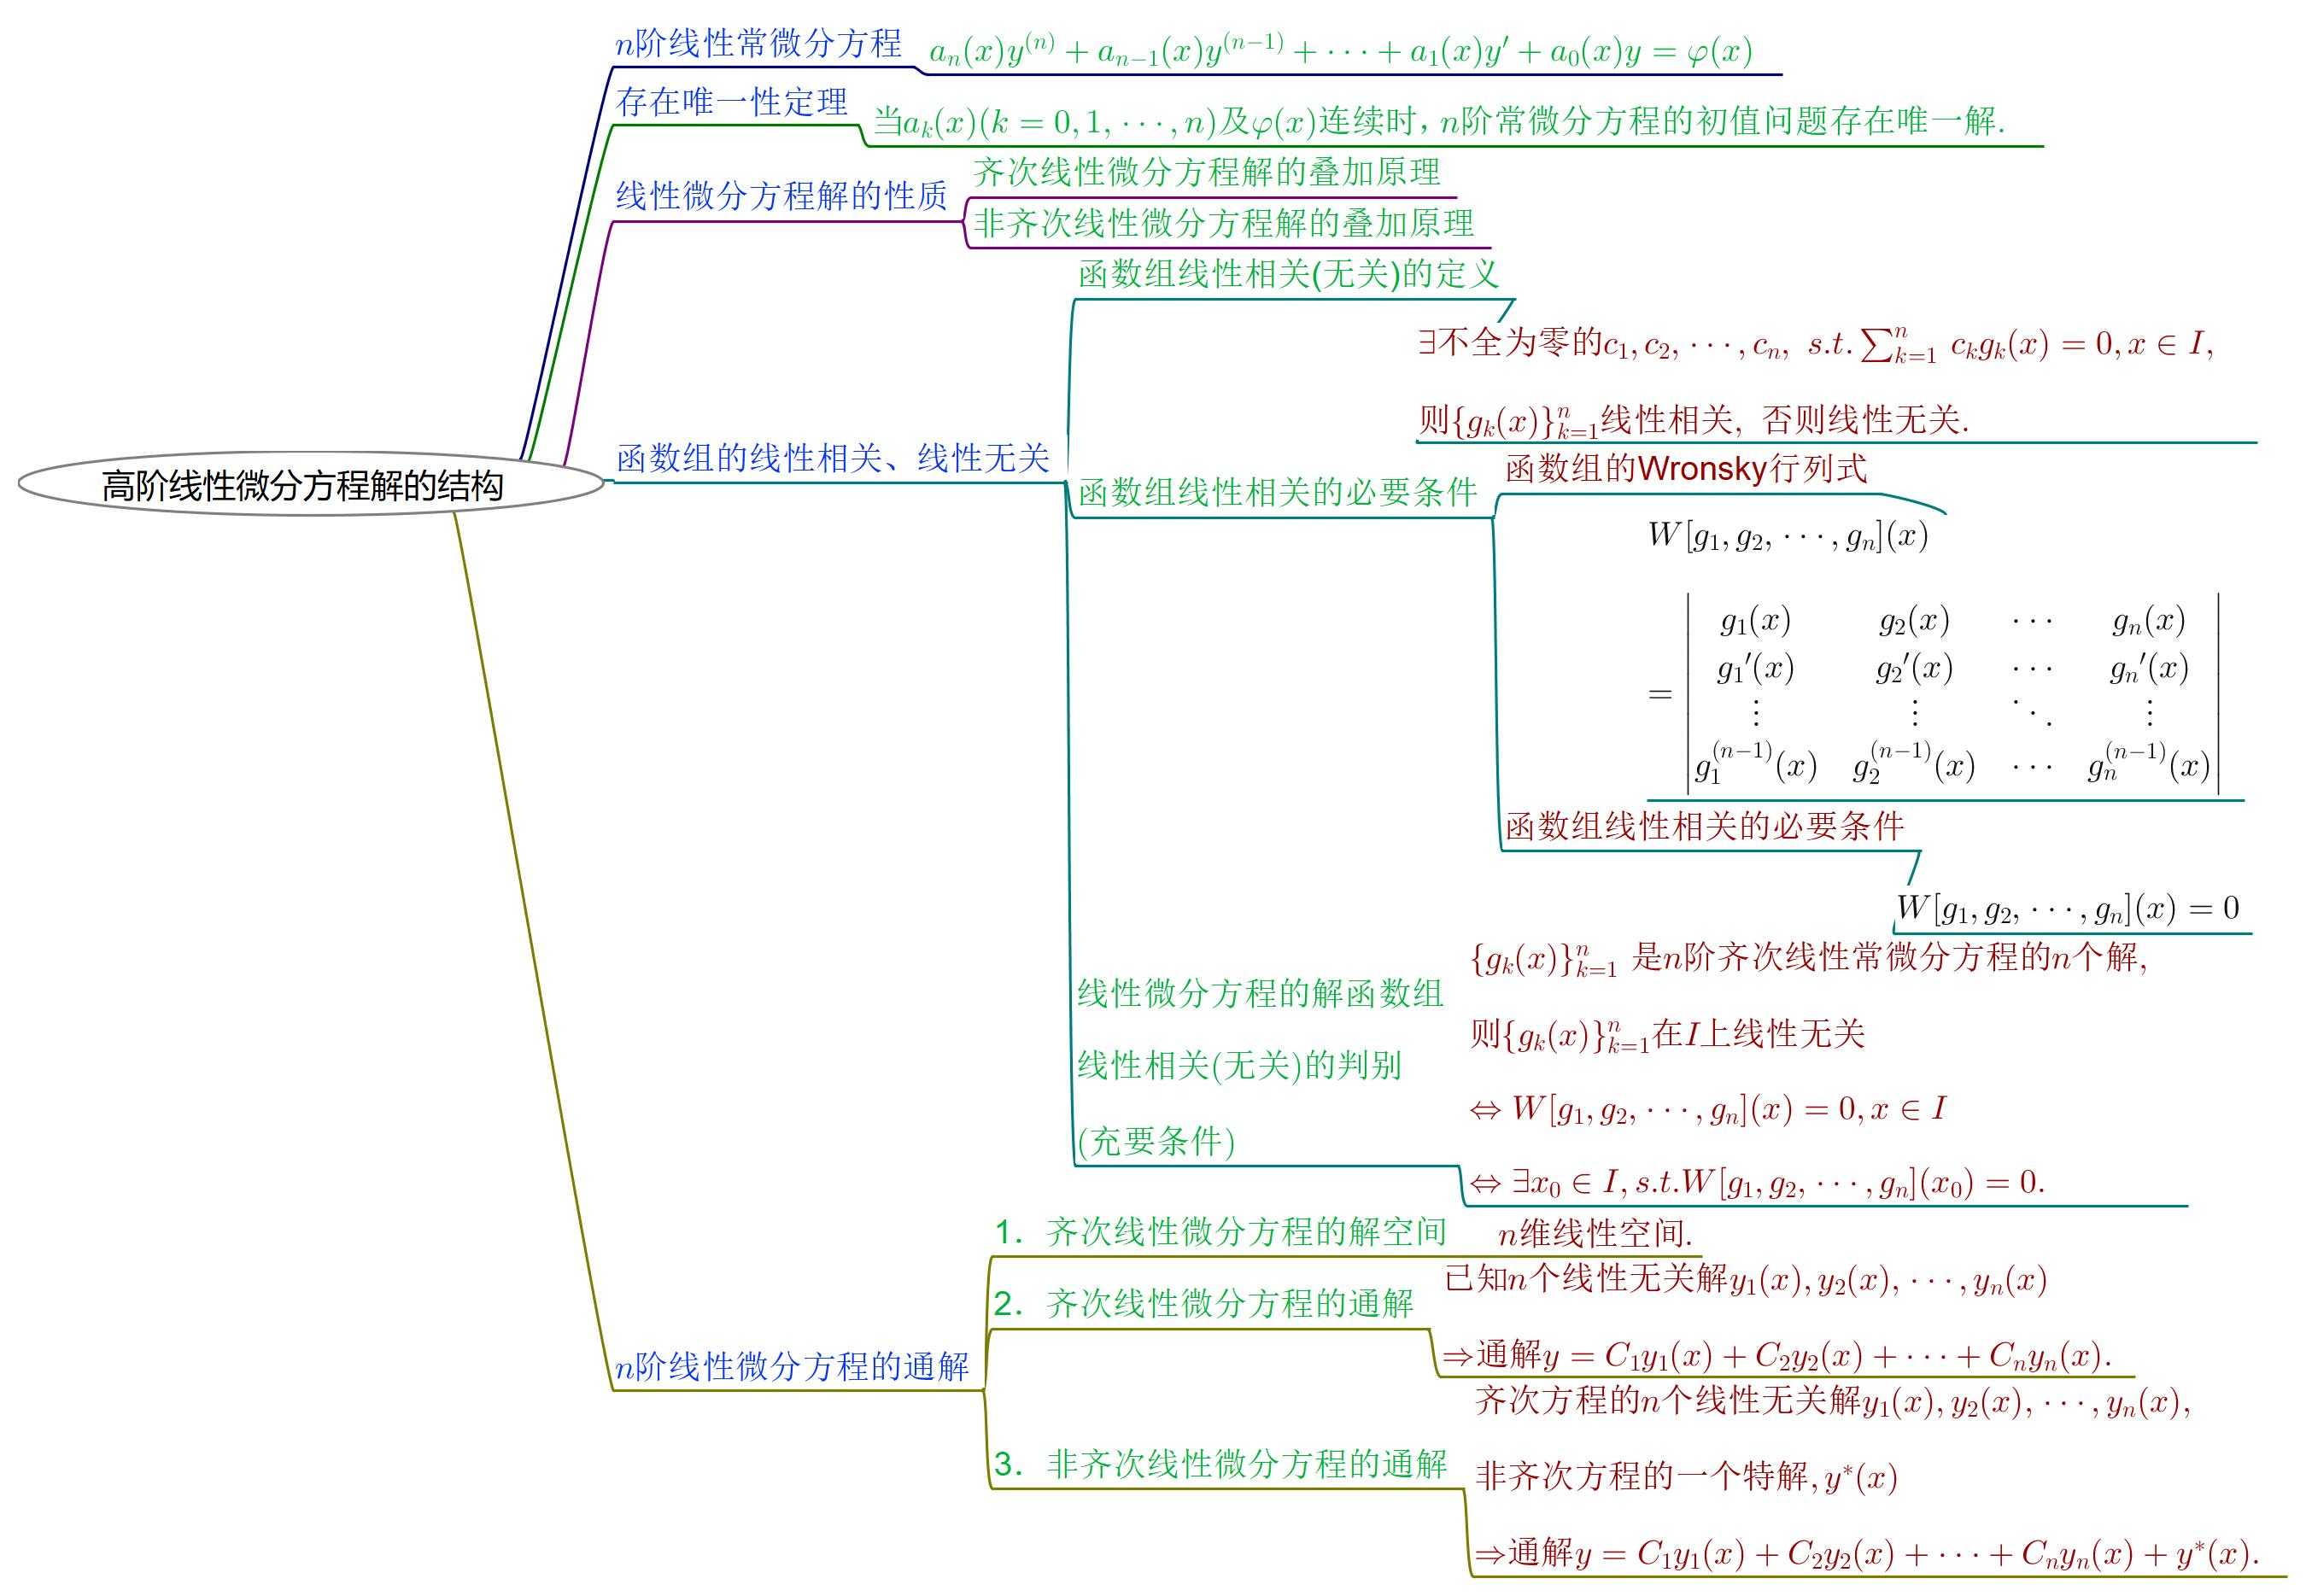
\includegraphics[height=0.5\textheight]{structures-1.jpg}
%\end{center}
%\end{figure}
\subsection{习题分类与解题思路}
\begin{enumerate}
\item判断函数组在定义区间内是否线性相关. 可参考以下思路:
\begin{enumerate}
\item[第一步]计算Wronsky行列式. 若Wronsky行列式不恒等于零,则函数组线性无关.

【如习题14.3中的1.(1)/(2)/(3)/(4)/(5)/(6).】
\item[第二步]若Wronsky行列式恒等于零,则可按照线性相关的定义,判断是否存在不全为零的$c_1,c_2,\cdots,c_n\in\mathbb R$使得$\sum_{i=1}^nc_ng_n(x)=0$,若存在则线性相关,若不存在则线性无关.

若已知函数组是$n$阶线性微分方程的解函数组,则由Wronsky行列式恒等于零,可直接得到该函数组线性相关.
\end{enumerate}
\item考查齐次和非齐次线性方程解的叠加原理. 

【如习题14.3中的3.】
\item考查线性微分方程解的存在唯一性定理.

【如习题14.3中的6.】
\item考查$n$阶线性微分方程的解函数组线性相关(无关)判别的充要条件.

【如习题14.3中的7.】
\item考查$n$阶齐次线性微分方程解的结构. $n$阶齐次线性微分方程的解空间是$n$维线性空间,找到该齐次线性微分方程的$n$个线性无关的解,就可写出该齐次线性微分方程的通解.

【如习题14.3中的2.】
\item考查$n$阶非齐次线性微分方程解的结构. 先确定该非齐次方程对应的齐次方程的$n$个线性无关的解,从而求出齐次方程的通解,加上该非齐次方程的一个特解即可得到该非齐次方程的通解.

【如习题14.3中的8.】
\item其他类型的题目. 利用Wronsky行列式证明$n$阶非齐次线性微分方程有$n+1$个线性无关的解.

【如习题14.3中的9.】
\end{enumerate}
\subsection{习题14.3解答}
\begin{enumerate}
\item判断下列函数组在其定义区间内是否线性相关:\\
\begin{tabular}{ll}
(1)$1,x,x^2,x^3,x^4$;&(2)$\me^{-x},1,\me^x$;\\
(3)$\me^x,x\me^x$;&(4)$\sin x,\cos x$;\\
(5)$\me^x\cos x,\me^x\sin x$;&(6)$\ln x,x\ln x$.
\end{tabular}

解:(1)$W[1,x,x^2,x^3,x^4](x)=\begin{vmatrix}
1&x&x^2&x^3&x^4\\
0&1&2x&3x^2&4x^3\\
0&0&2&6x&12x^2\\
0&0&0&6&24x\\
0&0&0&0&24\\
\end{vmatrix}=1\cdot1\cdot2\cdot6\cdot24\not\equiv0$,

故$1,x,x^2,x^3,x^4$线性无关.

(2)$W[\me^{-x},1,\me^x](x)=\begin{vmatrix}
\me^{-x}&1&\me^x\\
-\me^{-x}&0&\me^x\\
\me^{-x}&0&\me^x
\end{vmatrix}=(-1)^3(-\me^{-x}\me^x-\me^x\me^{-x})=2\not\equiv0$,

故$\me^{-x},1,\me^x$线性无关.

(3)$W[\me^x,x\me^x](x)=\begin{vmatrix}
\me^x&x\me^x\\
\me^x&\me^x(x+1)
\end{vmatrix}=\me^{2x}(x+1)-x\me^{2x}=\me^{2x}\not\equiv0$,

故$\me^x,x\me^x$线性无关.

(4)$W[\sin x,\cos x](x)=\begin{vmatrix}\sin x&\cos x\\\cos x&-\sin x\end{vmatrix}=-1\not\equiv0$,

故$\sin x,\cos x$线性无关.

(5)$W[\me^x\cos x,\me^x\sin x](x)=\begin{vmatrix}
\me^x\cos x&\me^x\sin x\\
\me^x(\cos x-\sin x)&\me^x(\sin x+\cos x)\\
\end{vmatrix}=\me^x(\sin x\cos x+\cos^2x-\sin x\cos x+\sin^2x)=\me^x\not\equiv0$,

故$\me^x\cos x,\me^x\sin x$线性无关.

(6)$W[\ln x,x\ln x](x)=\begin{vmatrix}\ln x&x\ln x\\ \frac1x&\ln x+1\end{vmatrix}=(\ln x+1)\ln x-\ln x=(\ln x)^2\not\equiv0$,

故$\ln x,x\ln x$线性无关.

\item验证$y_1=\me^{x^2}$与$y_2=x\me^{x^2}$都是方程$y''-4xy'+(4x^2-2)y=0$的解,并写出该方程的通解.

解:$y_1=\me^{x^2},y_1'=\me^{x^2}2x,y_1''=2\me^{x^2}+4x^2\me^{x^2}$,

$y_1''-4xy_1'+(4x^2-2)y_1=2\me^{x^2}+4x^2\me^{x^2}-4x\me^{x^2}2x+(4x^2-2)\me^{x^2}=\me^{x^2}(2+4x^2-8x^2+4x^2-2)=0$,

$y_2=x\me^{x^2},y_2'=\me^{x^2}(1+2x^2),y_2''=\me^{x^2}(4x+2x+4x^3)=\me^{x^2}(6x+4x^3)$,

$y_2''-4xy_2'+(4x^2-2)y_2=\me^{x^2}(6x+4x^3)-4x\me^{x^2}(1+2x^2)+(4x^2-2)x\me^{x^2}\\
=\me^{x^2}(6x+4x^3-4x-8x^3+4x^3-2x)=0$,

$\therefore y_1,y_2$都是二阶线性齐次微分方程$y''-4xy'+(4x^2-2)y=0$的解.

$\because W[y_1,y_2](x)=\begin{vmatrix}\me^{x^2}&x\me^{x^2}\\2x\me^{x^2}&\me^{x^2}(1+2x^2)\end{vmatrix}=\me^{2x^2}(1+2x^2)-2x^2\me^{x^2}=\me^{x^2}\not\equiv0$,

$\therefore y_1,y_2$线性无关, 二阶线性齐次微分方程的通解为$y=C_1y_1+C_2y_2=C_1\me^{x^2}+C_2x\me^{x^2}$.

\item验证$y=\frac1x(c_1\me^x+c_2\me^{-x})+\frac12\me^x$($c_1,c_2$是任意常数)是方程$xy''+2y'-xy=\me^x$的通解.

解:$y_1=\frac1x\me^x,y_1'=\frac{\me^x(x-1)}{x^2},y_1''=\frac{\me^x(x-1+1)x^2-\me^x(x-1)2x}{x^4}=\frac{\me^x(x^2-2x+2)}{x^3}$,

$xy_1''+2y_1'-xy_1=x\frac{\me^x(x^2-2x+2)}{x^3}+2\frac{\me^x(x-1)}{x^2}-x\frac1x\me^x=\frac{\me^x(x^2-2x+2+2x-2-x^2)}{x^2}=0$,

$y_2=\frac{\me^{-x}}x,y_2'=\frac{-\me^{-x}x-\me^{-x}}{x^2}=\frac{-\me^{-x}(x+1)}{x^2},y_2''=\frac{\me^{-x}(x+1-1)x^2+\me^{-x}(x+1)2x}{x^4}=\frac{\me^{-x}(x^2+2x+2)}{x^3}$,

$xy_2''+2y_2'-xy_2=x\frac{\me^{-x}(x^2+2x+2)}{x^3}+2\frac{-\me^{-x}(x+1)}{x^2}-x\frac{\me^{-x}}x=\frac{\me^{-x}(x^2+2x+2-2x-2-x^2)}{x^2}=0$,

$y_3=\frac12\me^x,y_3'=\frac12\me^x,y_3''=\frac12\me^x$,

$xy''+2y'-xy=(x+2-x)\frac12\me^x=\me^x$,

$\therefore$根据叠加定理$y=c_1y_1+c_2y_2+y_3=\frac1x(c_1\me^x+c_2\me^{-x})+\frac12\me^x$是方程$xy''+2y'-xy=\me^x$的通解.

%\item已知$y_1(x)=\me^x$是齐次方程$(2x-1)y''-(2x+1)y'+2y=0$的一个解,求该方程的通解.
%
%解:设$y=u(x)\me^x$是方程$(2x-1)y''-(2x+1)y'+2y=0$的解,
%
%$y'=\me^x(u'+u),y''=\me^x(u''+2u'+u)$,
%
%则$(2x-1)y''-(2x+1)y'+2y=(2x-1)\me^x(u''+2u'+u)-(2x+1)\me^x(u'+u)+2u\me^x\\
%=\me^x[(2x-1)u''+(4x-2-2x-1)u']+[(2x-1)(\me^x)''-(2x+1)(\me^x)'+2\me^x]u\\
%=\me^x[(2x-1)u''+(2x-3)u']=0$,
%
%$\therefore(2x-1)u''+(2x-3)u'=0$,
%
%令$p(x)=u'$,则$p'(x)=u''$,
%
%$\therefore(2x-1)p'+(2x-3)p=0$(*),
%
%当$p\not\equiv0$时$\frac{\md p}p=\frac{3-2x}{2x-1}\md x=(-1+\frac2{2x-1})\md x$,
%
%$\therefore\ln|p|=-x+\ln|2x-1|+C$,
%
%$\therefore p=\pm\me^C\me^{-x}(2x-1)$,
%
%$\because p\equiv0$也满足(*)式,
%
%$\therefore p=u'=C\me^{-x}(2x-1)$,
%
%$\therefore u=\int C\me^{-x}(2x-1)\md x=-C\me^{-x}(2x-1)+2C\int\me^{-x}\md x=-C\me^{-x}(2x-1)-2C\me^{-x}+C_1\\
%=C\me^{-x}(-2x+1-2)+C_1=C_2(2x+1)\me^{-x}+C_1$,
%
%$\therefore$原方程的通解为$y=[C_2(2x+1)\me^{-x}+C_1]\me^x=C_1\me^x+C_2(2x+1)$.
%
%\item已知$y_1(x)=\cos x,y_2(x)=\sin x$是齐次方程$y''+y=0$的两个解,求非齐次方程$y''+y=\sec x$的通解.
%
%解:由1.(4)知$y_1(x),y_2(x)$线性无关,故齐次方程$y''+y=0$的通解为\\$y=C_1\cos x+C_2\sin x$,
%
%设非齐次方程$y''+y=\sec x$的解为$y=C_1(x)\cos x+C_2(x)\sin x$,
%
%根据常数变易法$\begin{cases}C_1'(x)\cos x+C_2'(x)\sin x=0,\\-C_1'(x)\sin x+C_2'(x)\cos x=\sec x\end{cases}$, 解得$\begin{cases}
%C_1'(x)=\frac{-\tan x}{\cos^2x+\sin^2x}=-\tan x,\\
%C_2'(x)=\frac1{\cos^2x+\sin^2x}=1,
%\end{cases}$
%
%$\therefore\begin{cases}
%C_1(x)=-\int\tan x\md x=\ln|\cos x|+C_3,\\
%C_2(x)=\int\md x=x+C_4,
%\end{cases}$
%
%$\therefore$非齐次方程$y''+y=\sec x$的通解为$y=(\ln|\cos x|)\cos x+x\sin x+C_3\cos x+C_4\sin x$.

\item[6.]设$y=\varphi(x)$是方程$y''+p(x)y'+q(x)y=0$的一个不恒等于零的解,其中$p(x),q(x)$为$[a,b]$上的连续函数. 求证不存在$x_0\in(a,b)$, 使得$\varphi(x_0)=\varphi'(x_0)=0$.

证明:假设$\exists x_0\in(a,b),s.t.\varphi(x_0)=\varphi'(x_0)=0$,

$\because y\equiv0$也满足$y(x_0)=y'(x_0)=0$,

$\therefore$根据存在唯一性定理$\varphi(x)\equiv0$, 矛盾, 故假设不成立.

$\therefore$不存在$x_0\in(a,b)$, 使得$\varphi(x_0)=\varphi'(x_0)=0$.

\item[7.]设$p(x),q(x),r(x)$是区间$I$上的连续函数,$y_1(x),y_2(x),y_3(x)$是方程\[y'''(x)+p(x)y''(x)+q(x)y'(x)+r(x)y(x)=0\]的三个线性无关解,问是否存在$x_0\in I$,使得$y_1(x_0)=y_2(x_0)=y_3(x_0)=0$, 并说明理由.

解:假设存在$x_0\in I$,使得$y_1(x_0)=y_2(x_0)=y_3(x_0)=0$,

则$W[y_1,y_2,y_3](x_0)=\begin{vmatrix}y_1(x_0)&y_2(x_0)&y_3(x_0)\\ y_1'(x_0)&y_2'(x_0)&y_3'(x_0)\\y_1''(x_0)&y_2''(x_0)&y_3''(x_0)\end{vmatrix}=\begin{vmatrix}0&0&0\\ y_1'(x_0)&y_2'(x_0)&y_3'(x_0)\\y_1''(x_0)&y_2''(x_0)&y_3''(x_0)\end{vmatrix}=0$,

$\therefore$线性微分方程$y'''(x)+p(x)y''(x)+q(x)y'(x)+r(x)y(x)=0$的三个解$y_1(x),y_2(x),y_3(x)$线性相关,与题设矛盾,

$\therefore$不存在$x_0\in I$,使得$y_1(x_0)=y_2(x_0)=y_3(x_0)=0$.

\item[8.]设$y_1(x),y_2(x),y_3(x)$是方程\[y''(x)+p(x)y'(x)+q(x)y(x)=f(x)\]的三个特解,并且$\frac{y_2(x)-y_1(x)}{y_3(x)-y_1(x)}$不为常数. 求证$y(x)=(1-c_1-c_2)y_1(x)+c_1y_2(x)+c_2y_3(x)$是该方程的通解.

证明:$\because y_1(x),y_2(x),y_3(x)$是方程$y''(x)+p(x)y'(x)+q(x)y(x)=f(x)$的三个特解,

$\therefore$根据叠加定理$y_2(x)-y_1(x),\ y_3(x)-y_1(x)$是齐次方程$y''(x)+p(x)y'(x)+q(x)y(x)$的两个解, 

$\because\frac{y_2(x)-y_1(x)}{y_3(x)-y_1(x)}$不为常数,

$\therefore y_2(x)-y_1(x)$与$y_3(x)-y_1(x)$线性无关,

$\therefore$非齐次方程$y''(x)+p(x)y'(x)+q(x)y(x)=f(x)$的通解为
\[\begin{aligned}
y(x)&=c_1[y_2(x)-y_1(x)]+c_2[y_3(x)-y_1(x)]+y_1(x)\\
&=(1-c_1-c_2)y_1(x)+c_1y_2(x)+c_2y_3(x).
\end{aligned}\]
\item[9.]设函数$a_1(x),a_2(x),\cdots,a_n(x)$与$f(x)$连续,其中$f(x)\not\equiv0$,求证微分方程
\[y^{(n)}+a_1(x)y^{(n-1)}+\cdots+a_{n-1}(x)y'+a_n(x)y=f(x)\]
具有$n+1$个线性无关解,并用其$n+1$个线性无关解给出该方程的通解.

证明:设$\bar{y}_1(x),\bar{y}_2(x),\cdots,\bar{y}_n(x)$是齐次方程$y^{(n)}+a_1(x)y^{(n-1)}+\cdots+a_{n-1}(x)y'+a_n(x)y=0$的$n$个线性无关解,$\bar{y}$是非齐次方程$y^{(n)}+a_1(x)y^{(n-1)}+\cdots+a_{n-1}(x)y'+a_n(x)y=f(x)$的一个非零特解, 则$W[\bar y_1,\bar y_2,\cdots,\bar y_n](x)\not\equiv0$,

记$y_k(x)=\bar{y}_k(x)+\bar y(x),(k=1,2,\cdots,n)$, 则$y_k(x)$是非齐次方程的解,

则$W[y_1,y_2,\cdots,y_n,\bar y](x)\\
=W[\bar y_1,\bar y_2,\cdots,\bar y_n,\bar y](x)\\
=\begin{vmatrix}
\bar y_1(x)&\bar y_2(x)&\cdots&\bar y_n(x)&\bar y(x)\\
\bar y_1'(x)&\bar y_2'(x)&\cdots&\bar y_n'(x)&\bar y'(x)\\
\vdots&\vdots&\ddots&\vdots&\vdots\\
\bar y_1^{(n-1)}(x)&\bar y_2^{(n-1)}(x)&\cdots&y_{n}^{(n-1)}&\bar y^{(n-1)}(x)\\
\bar y_1^{(n)}(x)&\bar y_2^{(n)}(x)&\cdots&y_{n}^{(n)}&\bar y^{(n)}(x)
\end{vmatrix}$,

将该行列式的第$n-1$行$\times a_1(x)$,第$n-2$行$\times a_2(x),\cdots,$第$1$行$\times a_n(x)$加到第$n$行,考虑到$\bar y_k,k=1,2,\cdots,n$是齐次方程的解,$\bar y$是非齐次方程的解,得到

上式$=\begin{vmatrix}
\bar y_1(x)&\bar y_2(x)&\cdots&\bar y_n(x)&\bar y(x)\\
\bar y_1'(x)&\bar y_2'(x)&\cdots&\bar y_n'(x)&\bar y'(x)\\
\vdots&\vdots&\ddots&\vdots&\vdots\\
\bar y_1^{(n-1)}(x)&\bar y_2^{(n-1)}(x)&\cdots&y_{n}^{(n-1)}&\bar y^{(n-1)}(x)\\
0&0&\cdots&0&f(x)
\end{vmatrix}=f(x)W[\bar y_1,\bar y_2,\cdots,\bar y_n](x)\not\equiv0$,

$\therefore y_1(x),y_2(x),\cdots,y_n(x),\bar y(x)$线性无关,

故$y^{(n)}+a_1(x)y^{(n-1)}+\cdots+a_{n-1}(x)y'+a_n(x)y=f(x)$有$n+1$个线性无关解,

方程的通解为$y=C_1[y_1(x)-\bar y(x)]+C_2[y_2(x)-\bar y(x)]+\cdots+C_{n}[y_n(x)-\bar y(x)]+\bar y(x)$.
\end{enumerate}
\end{document}
\documentclass[12pt,UTF8]{ctexart}
\usepackage{ctex,amsmath,amssymb,geometry,fancyhdr,bm,amsfonts,mathtools,extarrows,graphicx,url,enumerate,color,float,multicol,subfig,wasysym} 
\allowdisplaybreaks[4]
% 加入中文支持
\newcommand\Set[2]{\left\{#1\ \middle\vert\ #2 \right\}}
\newcommand\Lim[0]{\lim\limits_{n\rightarrow\infty}}
\newcommand\LIM[2]{\lim\limits_{#1\rightarrow#2}}
\newcommand\Ser[1]{\sum_{n=#1}^\infty}
\newcommand{\SER}[2]{\sum_{#1=#2}^\infty}
\newcommand{\Int}[4]{\varint\nolimits_{#1}^{#2}#3\mathrm d#4}
\newcommand{\aIInt}[1]{\iint\limits_{#1}}
\newcommand{\IInt}[3]{\iint\limits_{#1}#2\mathrm d#3}
\newcommand{\varIInt}[4]{\iint\limits_{#1}#2\mathrm d#3\mathrm d#4}
\geometry{a4paper,scale=0.80}
\pagestyle{fancy}
\rhead{习题12.1\&12.2\&12.3}
\lhead{基础习题课讲义}
\chead{微积分B(2)}
\begin{document}
\setcounter{section}{17}
\section{重积分的概念和性质、二重积分的计算}
\subsection{知识结构}
\noindent第12章重积分
	\begin{enumerate}
		\item[12.1]二重积分的概念和性质
			\begin{enumerate}
				\item[12.1.1]引例(二重积分的几何意义)
					\begin{itemize}
						\item曲顶柱体的体积
						\item质量非均匀分布的平板质量
					\end{itemize}
				\item[12.1.2]二重积分的概念
				\item[12.1.3]二重积分的性质
					\begin{itemize}
						\item线性性质
						\item区域可加性
						\item保序性
						\item绝对值函数的可积性
						\item估值定理
						\item积分中值定理
						\item区域对称性
					\end{itemize}
			\end{enumerate}
		\item[12.2]二重积分的计算
			\begin{enumerate}
				\item[12.2.1]用直角坐标计算二重积分
				\item[12.2.2]用极坐标计算二重积分
			\end{enumerate}
		\item[12.3]二重积分的变量代换
	\end{enumerate}
\subsection{习题12.1解答}
\begin{enumerate}
\item利用重积分的几何意义求下列积分值:\\
(1)$\aIInt{D}\sqrt{R^2-x^2-y^2}\mathrm d\sigma,D=\Set{(x,y)}{x^2+y^2\leqslant R^2}$;\\
(2)$\aIInt{D}2\mathrm d\sigma,D=\Set{(x,y)}{x+y\leqslant1,y-x\leqslant1,y\geqslant0}$.

解:(1)$\aIInt{D}\sqrt{R^2-x^2-y^2}\mathrm d\sigma$的大小是曲面$z=\sqrt{R^2-x^2-y^2}$与平面$z=0$围成区域的体积,即等于半径为$a$的半球的体积,故
\[\aIInt{D}\sqrt{R^2-x^2-y^2}\mathrm d\sigma=\frac23\pi R^3.\]
(2)区域$D$的图形如图~\ref{1-2}所示,
\begin{figure}[H]
\begin{center}
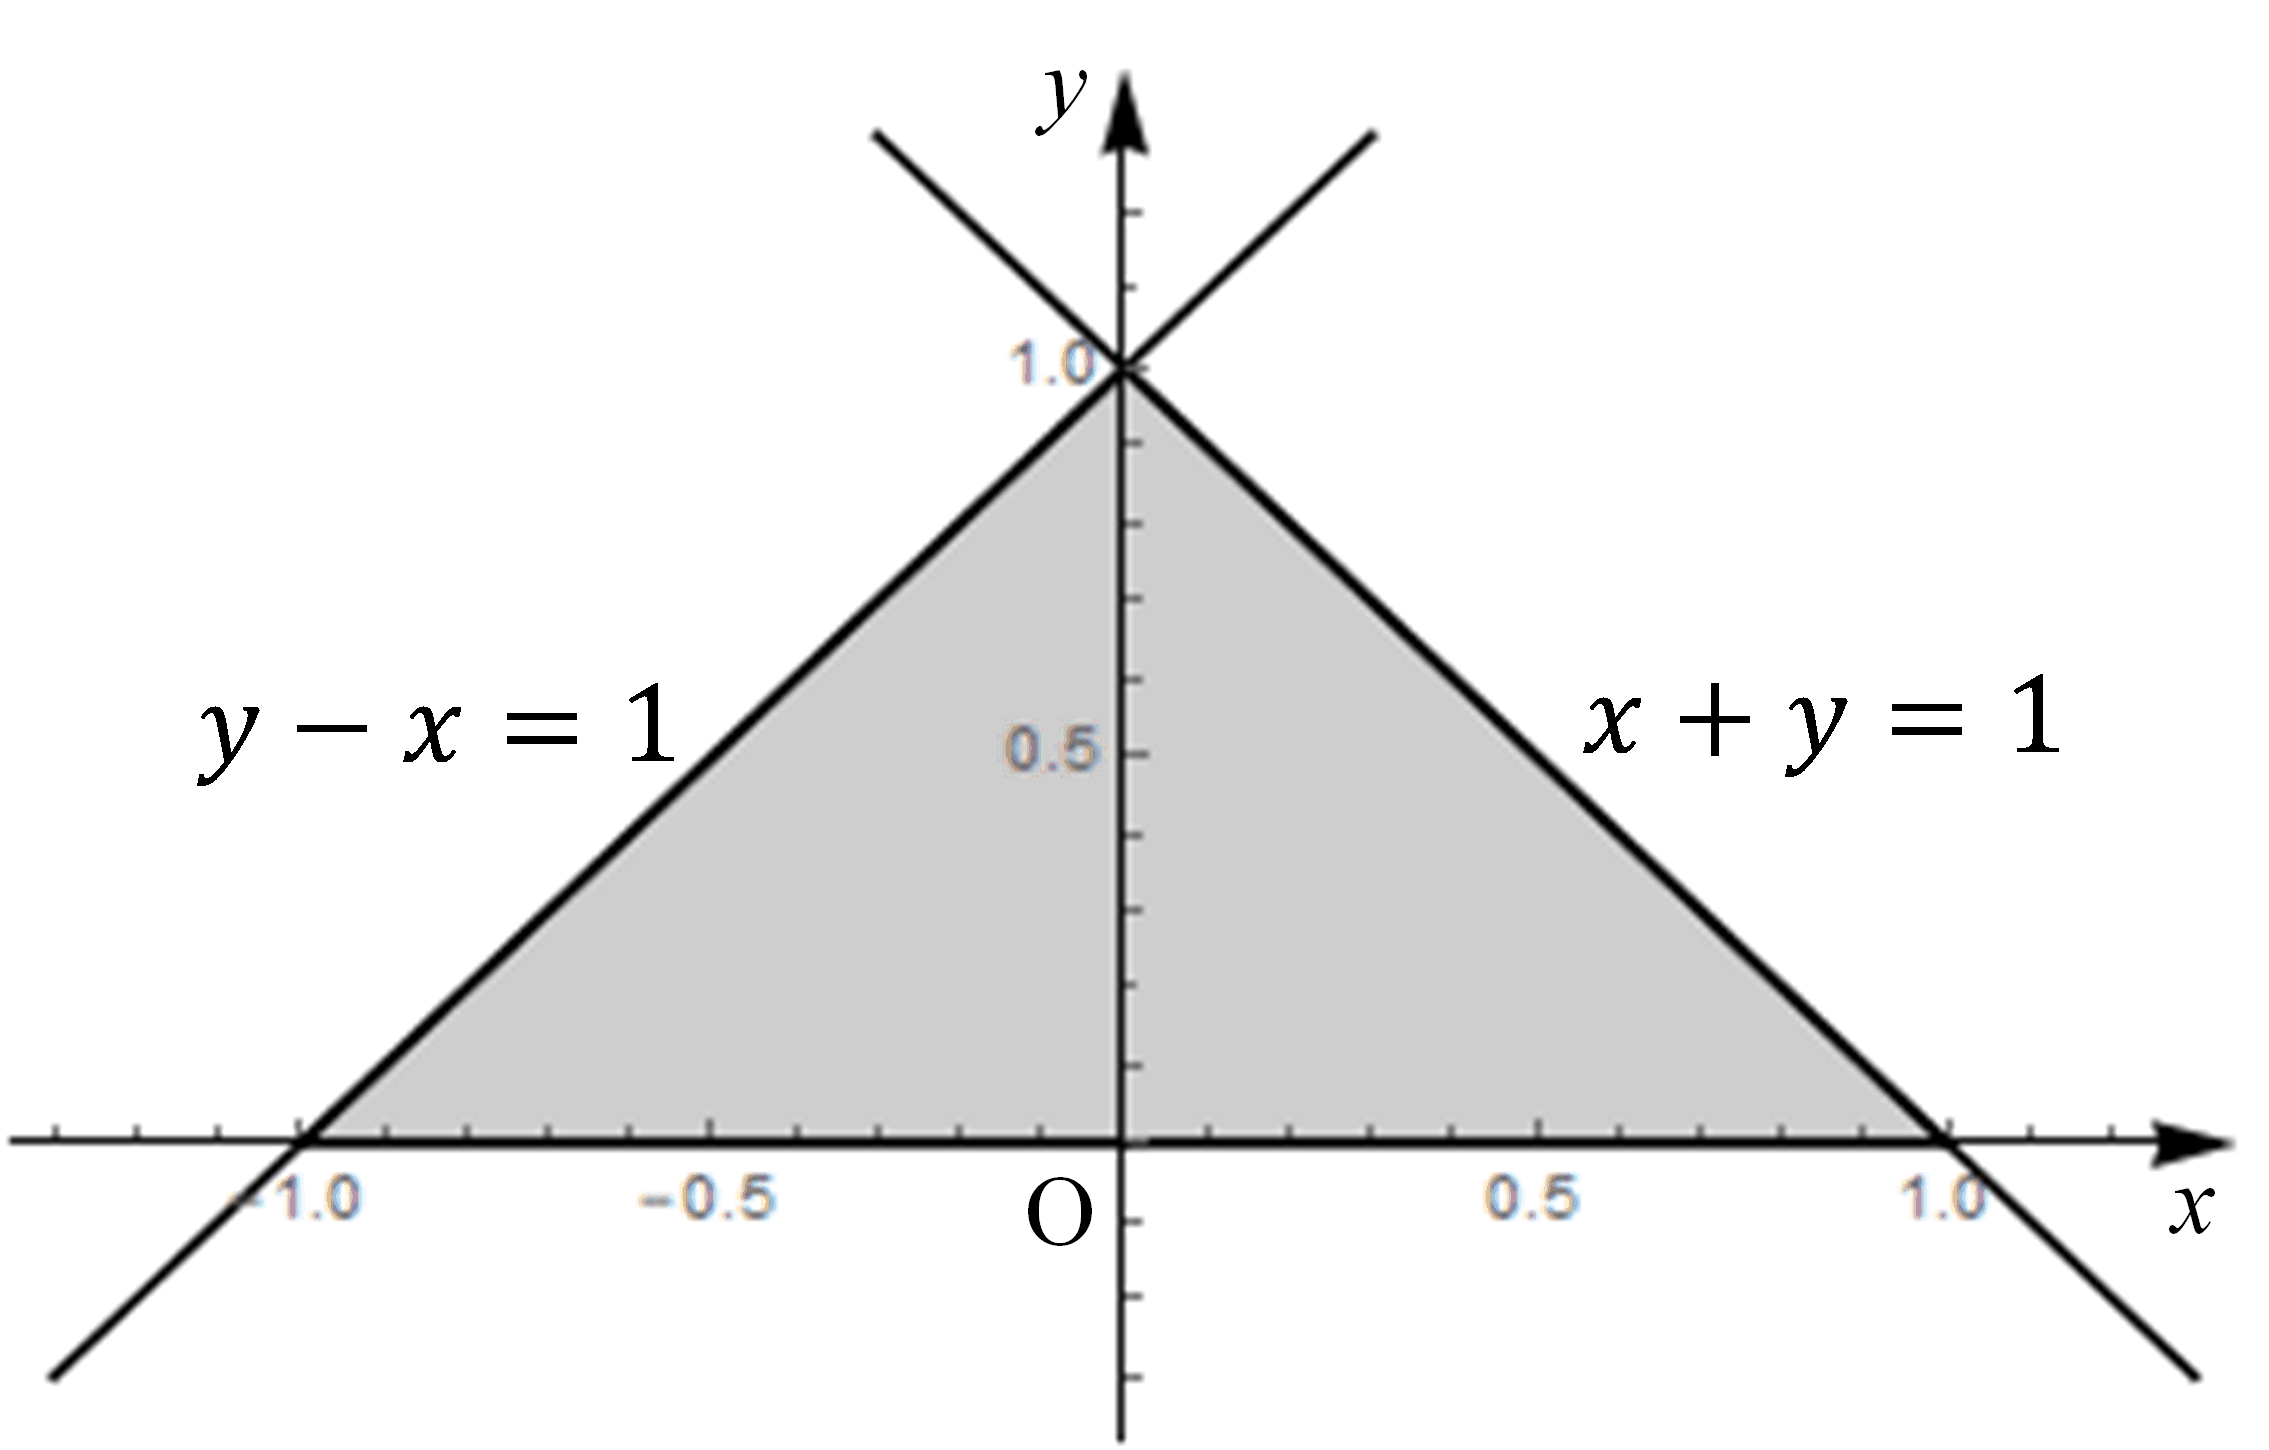
\includegraphics[height=0.2\textheight]{Figures/Fig1-2.png}
\end{center}
\caption{习题12.1 1.(2)题图示}
\label{1-2}
\end{figure}
积分$\aIInt{D}2\mathrm d\sigma$表示以区域$D$为底,高为$2$的棱柱体的体积,故
\[\aIInt{D}2\mathrm d\sigma=2\times(\frac12\times1\times2)=2.\]

\item利用重积分的性质估计下列积分值:\\
(1)$\aIInt{D}(1+y)x\mathrm d\sigma,D=\Set{(x,y)}{x^2+y^2\leqslant1,x\geqslant0,y\geqslant0}$;\\
(2)$\aIInt{D}(x^2+y^2)\mathrm d\sigma,D=\Set{(x,y)}{2x\leqslant x^2+y^2\leqslant4x}$.

解:(1)令$x=r\cos\theta,y=r\sin\theta$,则$D=\Set{(x,y)}{x^2+y^2\leqslant1,x\geqslant0,y\geqslant0}\\
=\Set{(r,\theta)}{0\leqslant r\leqslant1,0\leqslant\theta\leqslant\frac\pi2}$,

$\because$当$0\leqslant r\leqslant1,0\leqslant\theta\leqslant\frac\pi2$时,$0\leqslant\cos\theta\leqslant1,0\leqslant\sin2\theta\leqslant1$,

$\therefore(1+y)x=(1+r\sin\theta)r\cos\theta=r\cos\theta+r^2\sin\theta\cos\theta=r\cos\theta+\frac12r^2\sin2\theta\in[0,\frac32]$,

$\because\aIInt{D}\mathrm d\sigma=\frac\pi4$,

$\therefore0\leqslant\aIInt{D}(1+y)x\mathrm d\sigma\leqslant\frac32\aIInt{D}\mathrm d\sigma=\frac32\cdot\frac\pi4=\frac38\pi$,即$\aIInt{D}(1+y)x\mathrm d\sigma\in[0,\frac38\pi]$.

(2)方法1:$\because 2x\leqslant x^2+y^2\leqslant4x\Leftrightarrow\begin{cases}
x^2+y^2\geqslant2x,\\
x^2+y^2\leqslant4x,
\end{cases}\Leftrightarrow\begin{cases}
(x-1)^2+y^2\geqslant1,\\
(x-2)^2+y^2\leqslant4,
\end{cases}$

$\therefore$区域$D$如图~\ref{2-2}所示,
\begin{figure}[H]
\begin{center}
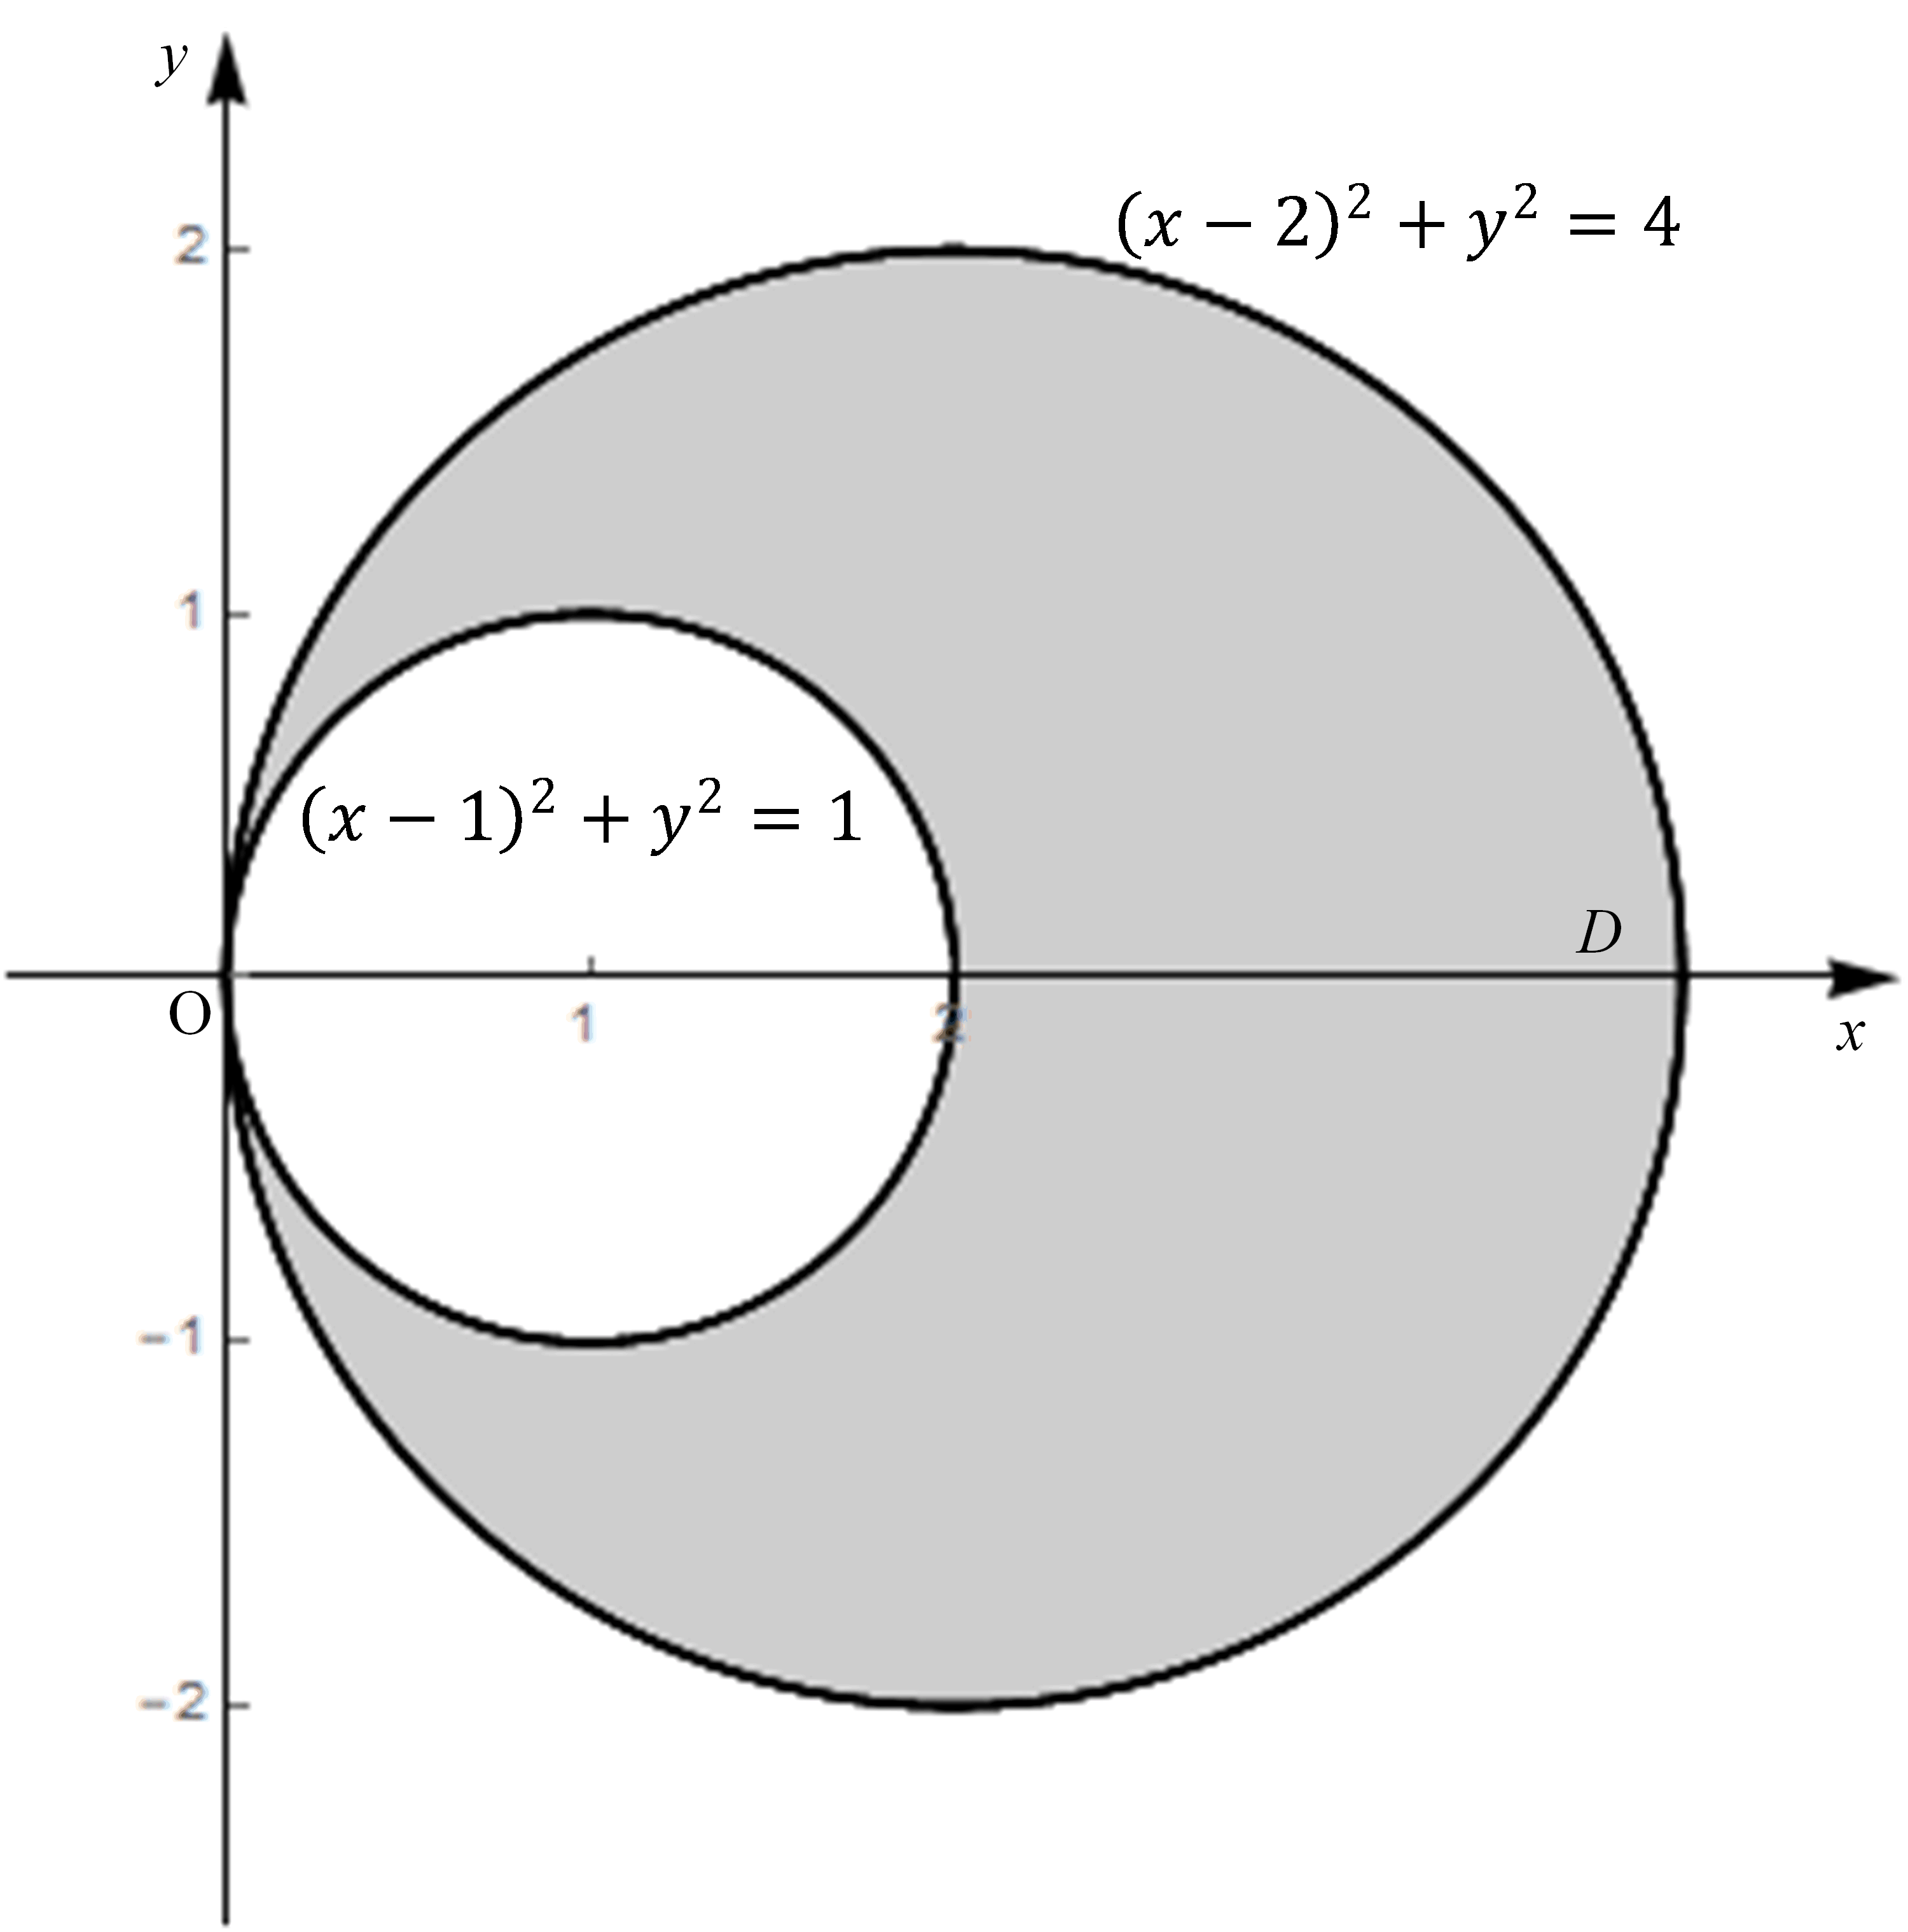
\includegraphics[height=0.3\textheight]{Figures/Fig2-2.png}
\end{center}
\caption{习题12.1 2.(2)题图示}
\label{2-2}
\end{figure}
由图~\ref{2-2}可知$0\leqslant x^2+y^2\leqslant4^2+0^2=16$,

$\because\aIInt{D}\mathrm d\sigma=2^2\pi-1^2\pi=3\pi$,

$\therefore0\leqslant\aIInt{D}(x^2+y^2)\mathrm d\sigma\leqslant16\aIInt{D}\mathrm d\sigma=48\pi$.

方法2:令$x=r\cos\theta,y=r\sin\theta$,则$D=\Set{(x,y)}{2x\leqslant x^2+y^2\leqslant4x}\\
=\Set{(r,\theta)}{2r\cos\theta\leqslant r^2\leqslant4r\cos\theta}=\Set{(r,\theta)}{2\cos\theta\leqslant r\leqslant4\cos\theta,0\leqslant\theta\leqslant2\pi}$,

$\therefore0\leqslant2\cos^2\theta\leqslant r^2\leqslant16\cos^2\theta\leqslant16$,即$0\leqslant x^2+y^2\leqslant4^2+0^2=16$,

$\because\aIInt{D}\mathrm d\sigma=2^2\pi-1^2\pi=3\pi$,

$\therefore0\leqslant\aIInt{D}(x^2+y^2)\mathrm d\sigma\leqslant16\aIInt{D}\mathrm d\sigma=48\pi$.

\item比较下列各组积分值的大小:\\
(1)$\aIInt{D}(x+y)^2\mathrm d\sigma$与$\aIInt{D}(x+y)^3\mathrm d\sigma$,其中$D=\Set{(x,y)}{(x-2)^2+(y-2)^2\leqslant2}$;\\
(2)$\aIInt{D}\ln(x+y)\mathrm d\sigma$与$\aIInt{D}xy\mathrm d\sigma$,其中$D$由直线$x=0,y=0,x+y=\frac12$及$x+y=1$围成.

解:(1)区域$D$的图形如图~\ref{3-1}所示,
\begin{figure}[H]
\begin{center}
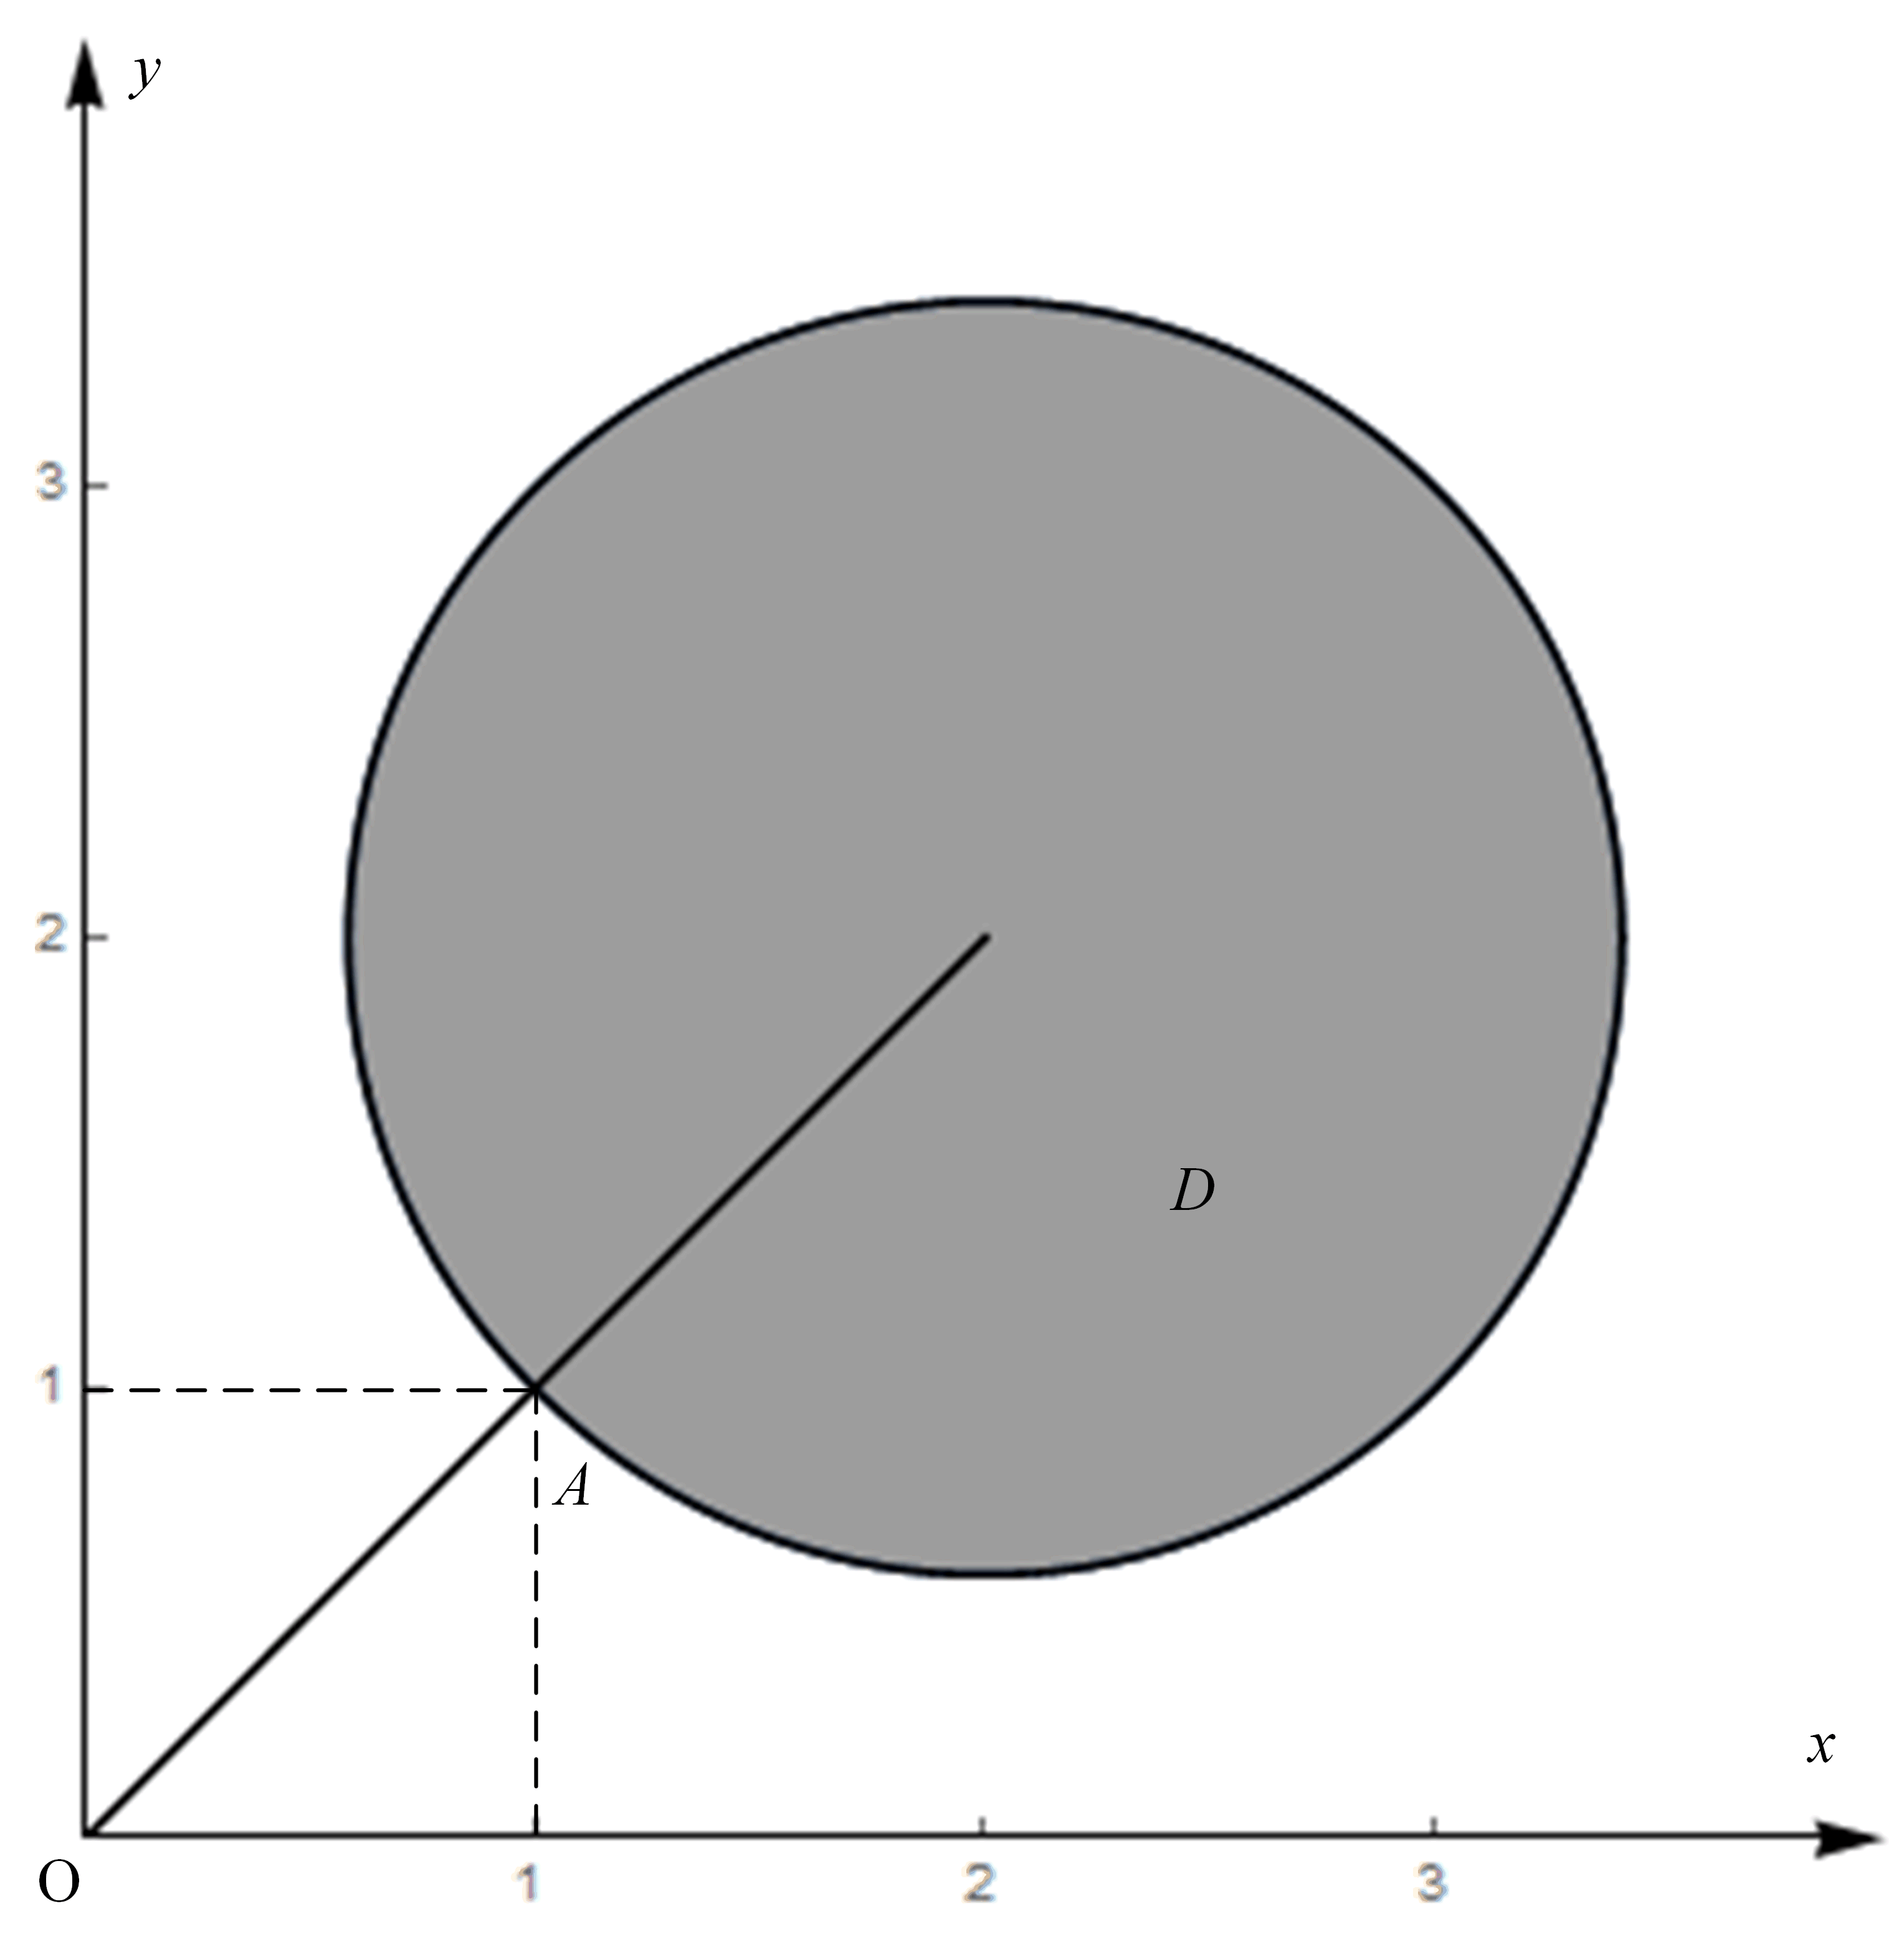
\includegraphics[height=0.3\textheight]{Figures/Fig3-1.png}
\end{center}
\caption{习题12.1 3.(1)题图示}
\label{3-1}
\end{figure}
由图~\ref{3-1}可知在区域$D$上$x+y>1$,则$(x+y)^2<(x+y)^3$,

$\therefore\aIInt{D}(x+y)^2\mathrm d\sigma<\aIInt{D}(x+y)^3\mathrm d\sigma$.

(2)区域$D$的图形如图~\ref{3-2}所示,
\begin{figure}[H]
\begin{center}
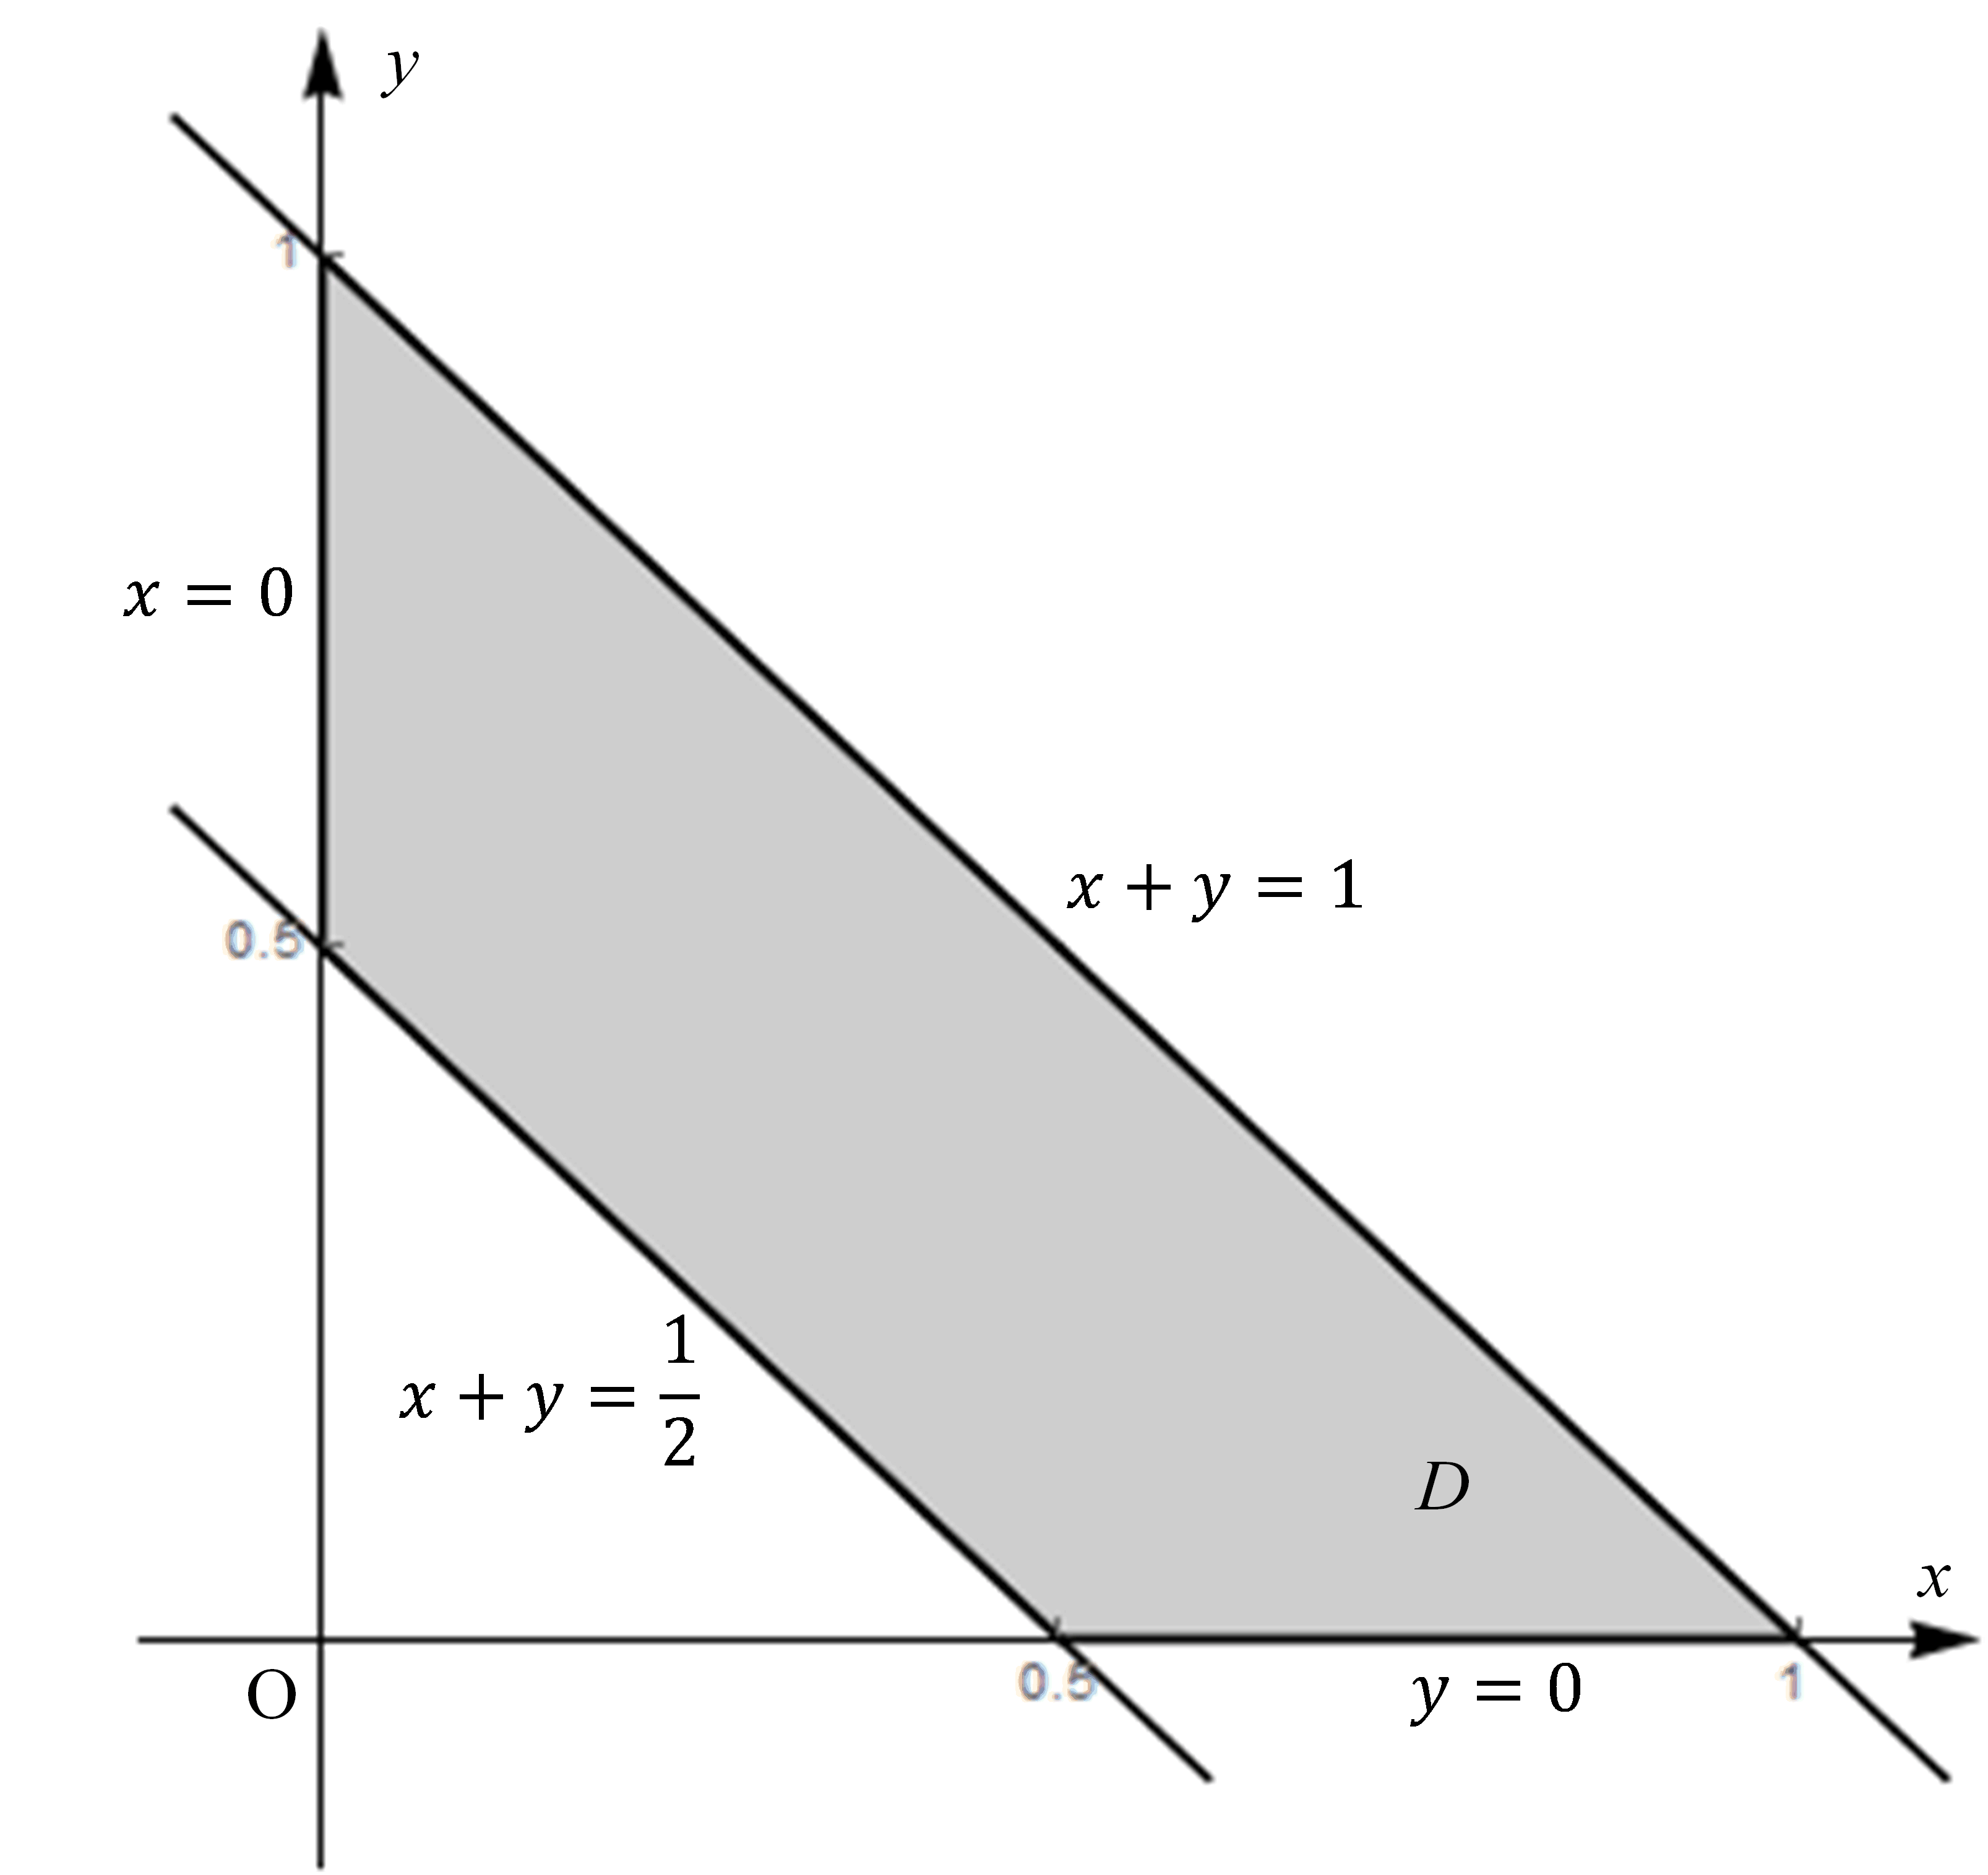
\includegraphics[height=0.3\textheight]{Figures/Fig3-2.png}
\end{center}
\caption{习题12.1 3.(2)题图示}
\label{3-2}
\end{figure}
由图~\ref{3-1}可知在区域$D$上$0<x+y\leqslant1$,则$\ln(x+y)\leqslant0\leqslant xy$,

$\therefore\aIInt{D}\ln(x+y)\mathrm d\sigma<0<\aIInt{D}xy\mathrm d\sigma$.

\item设$D\subset\mathbb R^2$是一有界闭域,$f(x,y)\in C(D)$且非负,试证:若$\aIInt{D}f(x,y)\mathrm d\sigma=0$,则\\
$f(x,y)\equiv0,\forall(x,y)\in D$.

证明:假设$f(x,y)$不恒为$0$,

$\because f(x,y)\in C(D)$且非负,

$\therefore\exists P(x_0,y_0)\in D$满足$f(x_0,y_0)>0$,且存在$P(x_0,y_0)$的一个邻域$N(P,\delta)$使得\\
$f(x,y)>\frac12f(x_0,y_0)>0$,

$\therefore\aIInt{D}f(x,y)\mathrm d\sigma=\aIInt{N(P,\delta)}f(x,y)\mathrm d\sigma+\aIInt{D\setminus N(P,\delta)}f(x,y)\mathrm d\sigma\geqslant\aIInt{N(P,\delta)}f(x,y)\mathrm d\sigma+0>0$,这与$\aIInt{D}f(x,y)\mathrm d\sigma=0$矛盾,

$\therefore$假设不成立,

$\therefore f(x,y)\equiv0,\forall(x,y)\in D$.
\item证明:若$f(x,y)\in C(D),g(x,y)\in R(D)$且不变号,则$\exists(\xi,\eta)\in D$使得
\[
\aIInt{D}f(x,y)g(x,y)\mathrm d\sigma=f(\xi,\eta)\aIInt{D}g(x,y)\mathrm d\sigma.
\]

证明:$\because f(x,y)\in C(D)$,

$\therefore\exists P,Q\in D,s.t.\ f(P)=m,f(Q)=M,\text{且}m\leqslant f(x,y)\leqslant M,\forall (x,y)\in D$,

$\because g(x,y)\in R(D)$且不变号,不妨设$g(x,y)\geqslant 0$,

$\therefore mg(x,y)\leqslant f(x,y)g(x,y)\leqslant Mg(x,y)$,

$\therefore m\aIInt{D}g(x,y)\mathrm d\sigma\leqslant\aIInt{D}f(x,y)g(x,y)\mathrm d\sigma\leqslant M\aIInt{D}g(x,y)\mathrm d\sigma$,

$\therefore$

i)当$\aIInt{D}g(x,y)\mathrm d\sigma=0$时$\aIInt{D}f(x,y)g(x,y)\mathrm d\sigma=0$,故$\aIInt{D}f(x,y)g(x,y)\mathrm d\sigma=f(\xi,\eta)\aIInt{D}g(x,y)\mathrm d\sigma$成立;

ii)当$\aIInt{D}g(x,y)\mathrm d\sigma\neq0$时$m\leqslant\frac{\aIInt{D}f(x,y)g(x,y)\mathrm d\sigma}{\aIInt{D}g(x,y)\mathrm d\sigma}\leqslant M$,由连续函数的介值定理知$\exists(\xi,\eta)\in D$满足
\[f(\xi,\eta)=\frac{\aIInt{D}f(x,y)g(x,y)\mathrm d\sigma}{\aIInt{D}g(x,y)\mathrm d\sigma},\]
即
\[\aIInt{D}f(x,y)g(x,y)\mathrm d\sigma=f(\xi,\eta)\aIInt{D}g(x,y)\mathrm d\sigma.\]
\item利用性质7的结论计算下列积分(其中区域$D$为圆盘$x^2+y^2\leqslant R^2$):\\
\begin{tabular}{ll}
(1)$\aIInt{D}y\sqrt{R^2-x^2}\mathrm d\sigma$;&(2)$\aIInt{D}y^3x^2\mathrm d\sigma$;\\
(3)$\aIInt{D}x^5\sqrt{R^2-y^2}\mathrm d\sigma$;&(4)$\aIInt{D}x^my^n\mathrm d\sigma$.
\end{tabular}

解:(1)因为区域$D$关于$x$轴对称,被积函数$f(x,y)=y\sqrt{R^2-x^2}=-f(x,-y)$关于$y$是奇函数,故$\aIInt{D}y\sqrt{R^2-x^2}\mathrm d\sigma=0$.

(2)因为区域$D$关于$x$轴对称,被积函数$f(x,y)=y^3x^2=-f(x,-y)$关于$y$是奇函数,故$\aIInt{D}y^3x^2\mathrm d\sigma=0$.

(3)因为区域$D$关于$y$轴对称,被积函数$f(x,y)=x^5\sqrt{R^2-y^2}=-f(-x,y)$关于$x$是奇函数,故$\aIInt{D}x^5\sqrt{R^2-y^2}\mathrm d\sigma=0$.

(4)区域$D$关于$x$轴和$y$轴均对称,

i)当$m$与$n$都是偶数时,$f(x,y)=x^my^n=f(-x,y)=f(x,-y)$关于$x$和$y$均是偶函数,故\\
$\aIInt{D}x^my^n\mathrm d\sigma=4\aIInt{D_1}x^my^n\mathrm d\sigma$,其中$D_1=\Set{(x,y)}{x^2+y^2\leqslant R^2,x\geqslant0,y\geqslant0}$;

ii)当$m$与$n$都是奇数时,$f(x,y)=x^my^n=-f(-x,y)$关于$x$是奇函数,$\aIInt{D}x^my^n\mathrm d\sigma=0$;

iii)当$m$是奇数$n$是偶数时,$f(x,y)=x^my^n=-f(-x,y)$关于$x$是奇函数,$\aIInt{D}x^my^n\mathrm d\sigma=0$;

iv)当$m$是偶数$n$是奇数时,$f(x,y)=x^my^n=-f(x,-y)$关于$y$是奇函数,$\aIInt{D}x^my^n\mathrm d\sigma=0$.

综上所述,当$m,n$均为偶数时,$\aIInt{D}x^my^n\mathrm d\sigma=4\aIInt{D_1}x^my^n\mathrm d\sigma$,其中$D_1$为区域$D$落在第一象限的部分;当$m,n$中至少有一个奇数时,$\aIInt{D}x^my^n\mathrm d\sigma=0$.
\end{enumerate}
\subsection{习题12.2解答}
\begin{enumerate}
\item计算下列二重积分:\\
(1)$\aIInt{D}\cos(x+y)\mathrm d\sigma,D$是由$x=0,y=\pi$和$y=x$围成的区域;\\
(2)$\aIInt{D}xy\ln(1+x^2+y^2)\mathrm d\sigma,D$是由$y=x^3,y=1$和$x=-1$围成的区域;\\
(3)$\aIInt{D}\sin(x+y)\mathrm d\sigma$,其中$D$由直线$x=0,y=x,y=\pi$围成;\\
(4)$\aIInt{D}|x^2-y|\mathrm d\sigma,D=\Set{(x,y)}{0\leqslant x,y\leqslant1}$;\\
(5)$\aIInt{D}\frac{x\sin y}y\mathrm d\sigma$,其中$D$由$y=x,y=x^2$围成.

解:(1)方法1:$\aIInt{D}\cos(x+y)\mathrm d\sigma=\Int{0}{\pi}{}{x}\Int{x}{\pi}{\cos(x+y)}{y}=\Int{0}{\pi}{\sin(x+y)\big|_x^\pi}{x}\\
=\Int{0}{\pi}{[\sin(x+\pi)-\sin2x]}{x}=\Int{0}{\pi}{(-\sin x-\sin2x)}{x}=\cos x\big|_0^\pi+\frac12\cos2x\big|_0^\pi\\
=-1-1+\frac12(1-1)=-2$.

方法2:$\aIInt{D}\cos(x+y)\mathrm d\sigma=\Int{0}{\pi}{}{y}\Int{0}{y}{\cos(x+y)}{x}=\Int{0}{\pi}{\sin(x+y)\big|_0^y}{y}\\
=\Int{0}{\pi}{(\sin2y-\sin x)}{y}=-\frac12\cos2y\big|_0^\pi+\cos x\big|_0^\pi=-\frac12(1-1)+(-1-1)=-2$.

(2)区域$D$如图~\ref{12-2-1-2}所示,
\begin{figure}[H]
\begin{center}
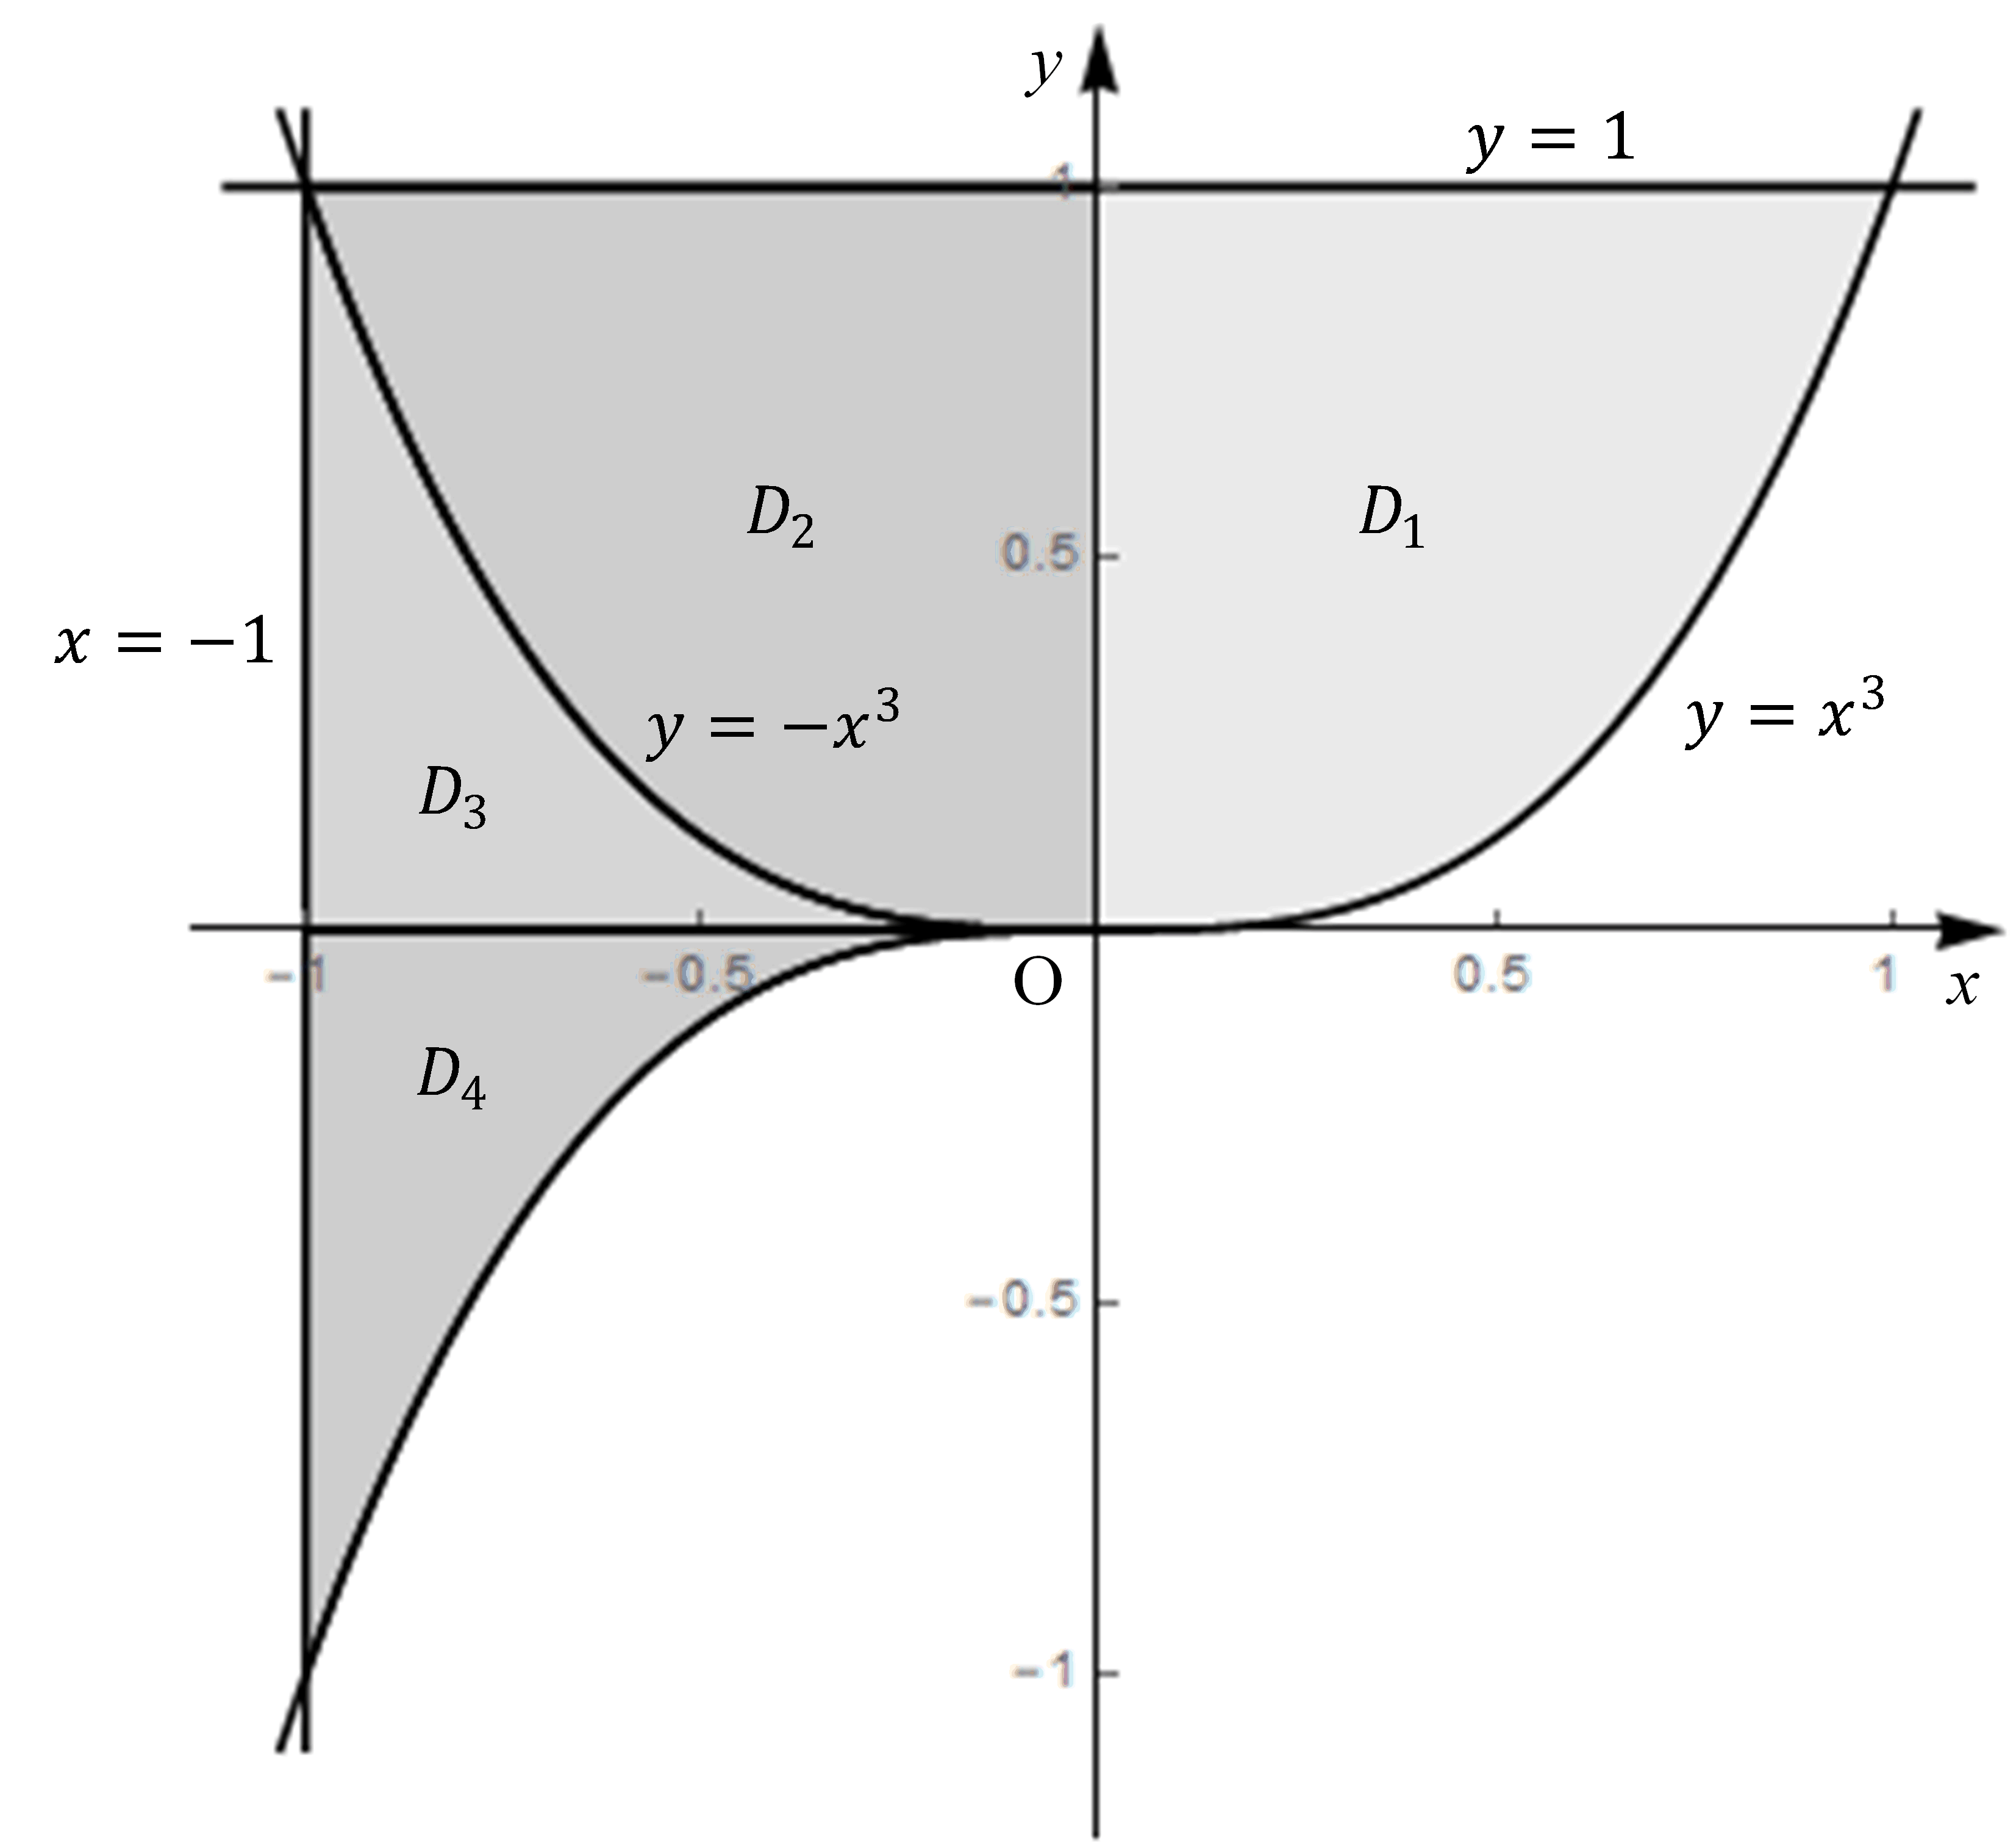
\includegraphics[height=0.3\textheight]{Figures/Fig12-2-1-2.png}
\end{center}
\caption{习题12.2 1.(2)题图示}
\label{12-2-1-2}
\end{figure}
可将区域$D$划分为图中的四个区域,其中$D_1$与$D_2$关于$y$轴对称,$D_3$与$D_4$关于$x$轴对称,被积函数$f(x,y)=xy\ln(1+x^2+y^2)$关于$x$和$y$均为奇函数,

$\therefore\IInt{D_1}xy\ln(1+x^2+y^2)\mathrm d\sigma+\IInt{D_2}xy\ln(1+x^2+y^2)\mathrm d\sigma=0,\\
\aIInt{D_3}xy\ln(1+x^2+y^2)\mathrm d\sigma+\aIInt{D_4}xy\ln(1+x^2+y^2)\mathrm d\sigma=0$,

$\therefore\aIInt{D}xy\ln(1+x^2+y^2)\mathrm d\sigma\\
=\aIInt{D_1}xy\ln(1+x^2+y^2)\mathrm d\sigma+\aIInt{D_2}xy\ln(1+x^2+y^2)\mathrm d\sigma+\aIInt{D_3}xy\ln(1+x^2+y^2)\mathrm d\sigma\\
+\aIInt{D_4}xy\ln(1+x^2+y^2)\mathrm d\sigma=0$.

(3)方法1:$\IInt{D}{\sin(x+y)}{\sigma}=\Int0\pi{}y\Int0y{\sin(x+y)}x=\Int0\pi{-\cos(x+y)\big|_0^y}y\\
=\Int0\pi{(-\cos y+\cos2y)}y=(-\sin y+\frac12\sin2y)\big|_0^\pi=0$.

方法2:$\IInt{D}{\sin(x+y)}{\sigma}=\Int0\pi{}x\Int x\pi{\sin(x+y)}x=\Int0\pi{-\cos(x+y)\big|_x^\pi}x\\
=\Int0\pi{[-\cos(\pi+x)+\cos2x]}x=\Int0\pi{(\cos x+\cos2x)}x=(\sin x+\frac12\sin2x)\big|_0^\pi=0$.

(4)将积分域$D$划分为以下两个区域$D_1=\Set{(x,y)}{0\leqslant x\leqslant1,0\leqslant y\leqslant x^2}$\\
和$D_2=\Set{(x,y)}{0\leqslant x\leqslant1,x^2\leqslant y\leqslant1}$,

则$\aIInt{D}|x^2-y|\mathrm d\sigma=\IInt{D_1}{(x^2-y)}\sigma+\IInt{D_2}{(y-x^2)}\sigma=\Int01{}x\Int0{x^2}{(x^2-y)}y+\Int01{}x\Int{x^2}1{(y-x^2)}y\\
=\Int10{(x^2y-\frac12y^2)\big|_0^{x^2}}x+\Int01{(\frac12y^2-x^2y)\big|_{x^2}^1}x=\Int10{(x^4-\frac12x^4)}x+\Int01{(\frac12-x^2-\frac12x^4+x^4)}x\\
=\Int01{(2x^4-x^4-x^2+\frac12)}x=\Int01{(x^4-x^2+\frac12)}x=(\frac15x^5-\frac13x^3+\frac12x)\big|_0^1=\frac15-\frac13+\frac12=\frac{11}{30}$.

(5)$\aIInt{D}\frac{x\sin y}y\mathrm d\sigma=\Int01{\frac{\sin y}y}y\Int y{\sqrt y}xx=\Int01{\frac{\sin y}y\frac12x^2\big|_y^{\sqrt y}}y=\Int01{\frac{\sin y}y\frac12(y-y^2)}y\\
=\frac12\Int01{(\sin y-y\sin y)}y=\frac12(-\cos y\big|_0^1+y\cos y\big|_0^1-\Int01{\cos y}y)\\
=\frac12(1-\cos1+\cos1-\sin y\big|_0^1)=\frac12(1-\sin 1)$.

注意:该题应先对$x$积分后对$y$积分,因$\frac{\sin y}{y}$无初等原函数,故不能先对$y$积分.

\item计算下列二重积分:\\
(1)$\IInt D{\sin\sqrt{x^2+y^2}}\sigma,D=\Set{(x,y)}{\pi^2\leqslant x^2+y^2\leqslant4\pi^2}$;\\
(2)$\IInt D{\frac1{1+x^2+y^2}}\sigma,D=\Set{(x,y)}{x^2+y^2\leqslant1}$;\\
(3)$\IInt D{\arctan\frac yx}\sigma,D=\Set{(x,y)}{1\leqslant x^2+y^2\leqslant4,x\geq0,y\geq0}$;\\
(4)$\IInt D{|x^2+y^2-4|}\sigma,D=\Set{(x,y)}{x^2+y^2\leqslant16}$.

解:(1)$\IInt D{\sin\sqrt{x^2+y^2}}\sigma=\Int0{2\pi}{}\theta\Int\pi{2\pi}{r\sin r}r=2\pi(-r\cos r\big|_\pi^{2\pi}+\Int\pi{2\pi}{\cos r}r)\\
=2\pi(-2\pi-\pi+\sin r\big|_\pi^{2\pi})=-6\pi^2$.

(2)$\IInt D{\frac1{1+x^2+y^2}}\sigma=\Int0{2\pi}{}\theta\Int01{\frac r{1+r^2}}r=\pi\ln(1+r^2)\big|_0^1=\pi\ln2$.

(3)$\IInt D{\arctan\frac yx}\sigma=\Int0{\frac\pi2}{}\theta\Int12{r\arctan(\frac{r\sin\theta}{r\cos\theta})}r=\Int0{\frac\pi2}{\theta}\theta\Int12{r}r=(\frac12\theta^2\big|_0^{\frac\pi2})(\frac12r^2\big|_1^2)=\frac{3\pi^2}{16}$.

(4)$\IInt D{|x^2+y^2-4|}\sigma=\Int0{2\pi}{}\theta\Int04{|r^2-4|r}r=\Int0{2\pi}{}\theta[\Int02{(4r-r^3)}r+\Int24{(r^3-4r)}r]\\
=2\pi[(2r^2-\frac14r^4)\big|_0^2+(\frac14r^4-2r^2)\big|_2^4]=2\pi(8-4+64-32-4+8)=80\pi$.

\item改变下列累次积分中的积分顺序,并给出相应重积分的积分域的集合表示:\\
\begin{tabular}{ll}
(1)$\Int01{}y\Int0y{f(x,y)}x$;&(2)$\Int{-1}1{}x\Int{-\sqrt{1-x^2}}{\sqrt{1-x^2}}{f(x,y)}y$;\\
(3)$\Int0a{}x\Int{a-x}{\sqrt{a^2-x^2}}{f(x,y)}y$;&(4)$\Int1{\mathrm e}{}x\Int0{\ln x}{f(x,y)}y$.
\end{tabular}

解:(1)积分域$D=\Set{(x,y)}{0\leqslant y\leqslant1,0\leqslant x\leqslant y}=\Set{(x,y)}{0\leqslant x\leqslant1,x\leqslant y\leqslant1}$,

则$\Int01{}y\Int0y{f(x,y)}x=\Int01{}x\Int x1{f(x,y)}y$.

(2)积分域$D=\Set{(x,y)}{-1\leqslant x\leqslant1,-\sqrt{1-x^2}\leqslant y\leqslant\sqrt{1-x^2}}\\
=\Set{(x,y)}{-1\leqslant y\leqslant1,-\sqrt{1-y^2}\leqslant x\leqslant\sqrt{1-y^2}}=\Set{(x,y)}{x^2+y^2\leq1}$,

则$\Int{-1}1{}x\Int{-\sqrt{1-x^2}}{\sqrt{1-x^2}}{f(x,y)}y=\Int{-1}1{}y\Int{-\sqrt{1-y^2}}{\sqrt{1-y^2}}{f(x,y)}x$.

(3)积分域$D=\Set{(x,y)}{0\leqslant x\leqslant a,a-x\leqslant y\leqslant\sqrt{a^2-x^2}}\\
=\Set{(x,y)}{0\leqslant y\leqslant a,a-y\leqslant x\leqslant\sqrt{a^2-y^2}}\\
=\Set{(x,y)}{\text{直线$x+y=a$与圆$x^2+y^2=a^2$在第一象限围成的部分}}$,

则$\Int0a{}x\Int{a-x}{\sqrt{a^2-x^2}}{f(x,y)}y=\Int0a{}y\Int{a-y}{\sqrt{a^2-y^2}}{f(x,y)}x$.

(4)积分域$D=\Set{(x,y)}{1\leqslant x\leqslant\mathrm e,0\leqslant y\leqslant\ln x}=\Set{(x,y)}{0\leqslant y\leqslant1,\mathrm e^y\leqslant x\leqslant\mathrm e}$,

则$\Int1{\mathrm e}{}x\Int0{\ln x}{f(x,y)}y=\Int01{}y\Int{\mathrm e^y}{\mathrm e}{f(x,y)}x$.

\item将下列累次积分交换积分顺序:\\
\begin{tabular}{ll}
(1)$\Int0a{}x\Int x{\sqrt{2ax-x^2}}{f(x,y)}y$;&(2)$\Int{-6}2{}x\Int{\frac14x^2-1}{2-x}{f(x,y)}y$.
\end{tabular}

解:(1)积分域$D=\Set{(x,y)}{0\leqslant x\leqslant a,x\leqslant y\leqslant\sqrt{2ax-x^2}}\\
=\Set{(x,y)}{0\leqslant y\leqslant a,a-\sqrt{a^2-y^2}\leqslant x\leqslant y}$,

则$\Int0a{}x\Int x{\sqrt{2ax-x^2}}{f(x,y)}y=\Int0a{}y\Int{a-\sqrt{a^2-y^2}}y{f(x,y)}x$.

(2)积分域$D=\Set{(x,y)}{-6\leqslant x\leqslant2,\frac14x^2-1\leqslant y\leqslant2-x}\\
=\Set{(x,y)}{0\leqslant y\leqslant8,-2\sqrt{1+y}\leqslant x\leqslant2-y}\cup\Set{(x,y)}{-1\leqslant y\leqslant0,-2\sqrt{1+y}\leqslant x\leqslant2\sqrt{1+y}}$,

则$\Int{-6}2{}x\Int{\frac14x^2-1}{2-x}{f(x,y)}y=\Int08{}y\Int{-2\sqrt{1+y}}{2-y}{f(x,y)}x+\Int{-1}0{}y\Int{-2\sqrt{1+y}}{2\sqrt{1+y}}{f(x,y)}x$.

\item已知函数$f$连续且$f>0$,试求$\IInt D{\frac{af(x)+bf(y)}{f(x)+f(y)}}\sigma$的值,其中$D=\Set{(x,y)}{x^2+y^2\leqslant R^2}$.

解:$\because$积分域$D$关于$y=x$对称,且在关于$y=x$的对称点$(x,y)$和$(x',y')=(y,x)$处\\
$\frac{f(x')}{f(x')+f(y')}=\frac{f(y)}{f(y)+f(x)}$,

$\therefore\varIInt D{\frac{f(x)}{f(x)+f(y)}}xy=\varIInt D{\frac{f(y)}{f(x)+f(y)}}xy=\frac12\varIInt D{\frac{f(x)+f(y)}{f(x)+f(y)}}xy=\frac12\varIInt D{}xy=\frac12\pi R^2$,

$\therefore\varIInt D{\frac{af(x)+bf(y)}{f(x)+f(y)}}xy=a\varIInt D{\frac{f(x)}{f(x)+f(y)}}xy+b\varIInt D{\frac{f(y)}{f(x)+f(y)}}xy=\frac{a+b}2\pi R^2$.

%解:$\because$积分域$D$关于$y=x$对称,且在关于$y=x$的对称点$(x,y)$和$(y,x)$处\\
%$\frac{f(x)}{f(x)+f(y)}=\frac{f(y)}{f(x)+f(y)}$,
%
%$\therefore\IInt D{\frac{f(x)}{f(x)+f(y)}}\sigma=\IInt D{\frac{f(y)}{f(x)+f(y)}}\sigma$,
%
%$\because\IInt D{\frac{f(x)}{f(x)+f(y)}}\sigma+\IInt D{\frac{f(y)}{f(x)+f(y)}}\sigma=\IInt D{\frac{f(x)+f(y)}{f(x)+f(y)}}\sigma=\IInt D{}\sigma=\pi R^2$,
%
%$\therefore\IInt D{\frac{f(x)}{f(x)+f(y)}}\sigma=\IInt D{\frac{f(y)}{f(x)+f(y)}}\sigma=\frac\pi2 R^2$,
%
%$\therefore\IInt D{\frac{af(x)+bf(y)}{f(x)+f(y)}}\sigma=a\IInt D{\frac{f(x)}{f(x)+f(y)}}\sigma+b\IInt D{\frac{f(y)}{f(x)+f(y)}}\sigma=\frac{a+b}2\pi R^2$.
\end{enumerate}
\subsection{习题12.3解答}
\begin{enumerate}
\item求由$xy=a^2,xy=2a^2,y=x,y=2x$围成的第一象限区域的面积.

解:令$\begin{cases}
u=xy,\\
v=\frac yx,
\end{cases}$所求区域$D=\Set{(u,v)}{a^2\leqslant u\leqslant2a^2,1\leqslant v\leqslant2}$,

$\frac{\mathrm D(u,v)}{\mathrm D(x,y)}=\begin{vmatrix}
y&x\\
-\frac y{x^2}&\frac1x
\end{vmatrix}=\frac yx+\frac yx=2v,\ |\frac{\mathrm D(x,y)}{\mathrm D(u,v)}|=\frac1{2v}$,

所求面积$S=\IInt D{}\sigma=\varIInt D{|\frac{\mathrm D(x,y)}{\mathrm D(u,v)}|}uv=\Int{a^2}{2a^2}{}u\Int12{\frac1{2v}}v=a^2\frac12\ln v\big|_1^2=\frac{\ln2}2a^2$.

\item计算$I=\IInt D{\cos(\frac{x-y}{x+y})}\sigma,D$由$x+y=1,x=0,y=0$围成.

解:方法1:$\because$区域$D$关于$y=x$对称,且在关于$y=x$的对称点$(x,y)$和$(y,x)$处$\cos(\frac{x-y}{x+y})=\cos(\frac{y-x}{y+x})$,

$\therefore I=\IInt D{\cos(\frac{x-y}{x+y})}\sigma=2\IInt{D_1}{\cos(\frac{x-y}{x+y})}\sigma$,其中区域$D_1$由$x+y=1,y=0,y=x$围成.

令$\begin{cases}
u=x+y,\\
v=\frac yx,
\end{cases}$则$\begin{cases}
x=\frac u{1+v},\\
y=\frac{uv}{1+v},
\end{cases}$区域$D_1=\Set{(u,v)}{0\leqslant u\leqslant1,0\leqslant v\leqslant1}$,

$\frac{\mathrm D(u,v)}{\mathrm D(x,y)}=\begin{vmatrix}
1&1\\
-\frac y{x^2}&\frac1x
\end{vmatrix}=\frac{x+y}{x^2}=\frac{(1+v)^2}u,\ |\frac{\mathrm D(u,v)}{\mathrm D(x,y)}|=\frac u{(1+v)^2}$,

$\therefore I=2\IInt{D_1}{\cos(\frac{x-y}{x+y})}\sigma=2\varIInt{D_1}{\cos(\frac{1-v}{1+v})\frac u{(1+v)^2}}uv=2\Int01{\cos(\frac{1-v}{1+v})\frac1{(1+v)^2}}v\Int01uu\\
=\Int01{\cos(\frac{1-v}{1+v})\frac1{(1+v)^2}}v=\Int01{\cos(-1+\frac2{1+v})\frac1{(1+v)^2}}v=-\frac12\Int01{\cos(-1+\frac2{1+v})}{(-1+\frac2{1+v})}\\
=-\frac12\sin(-1+\frac2{1+v})\big|_0^1=\frac12\sin1$.

{\bf注}:如图\ref{12-3-2-1}所示.\footnotemark\footnotetext{这是修订版增加的内容.}
\begin{figure}[H]
\begin{center}
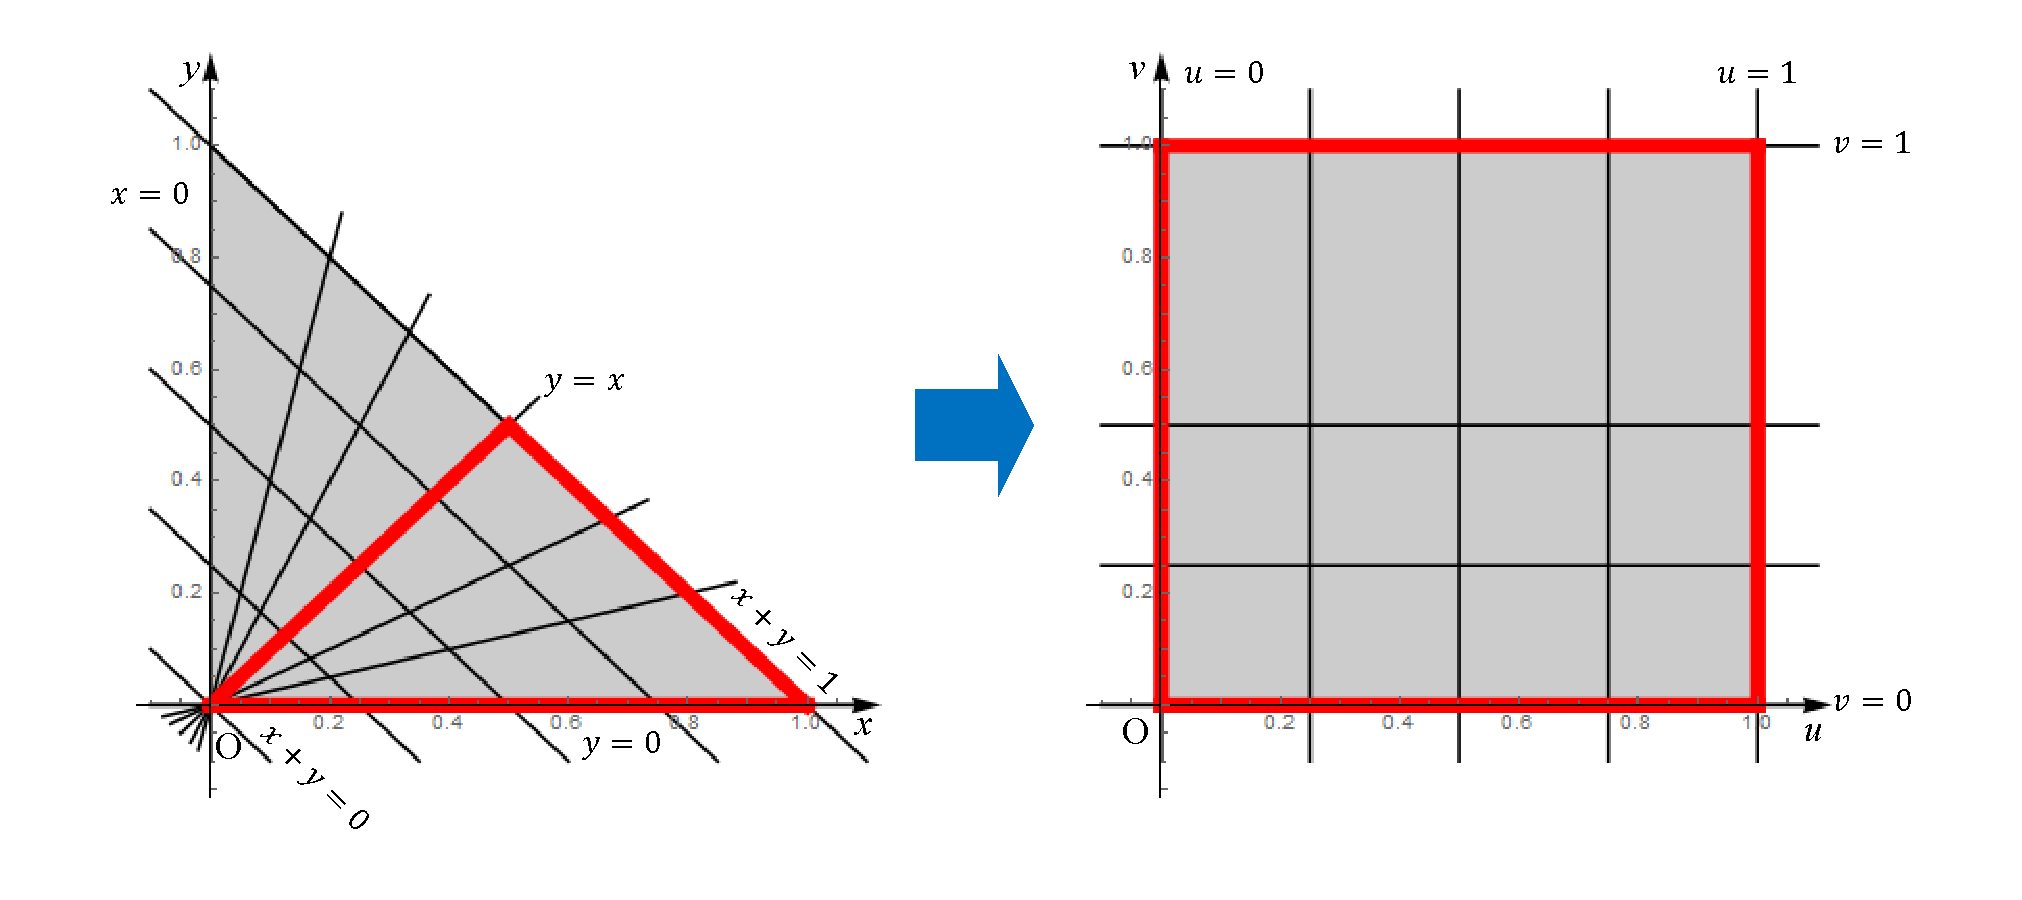
\includegraphics[height=0.3\textheight]{Figures/Fig12-3-2-1.pdf}
\end{center}
\caption{习题12.3 2题方法1图示}
\label{12-3-2-1}
\end{figure}

方法2:令$\begin{cases}
x=r\cos^2\theta,\\
y=r\sin^2\theta,
\end{cases}$则区域$D=\Set{(x,y)}{0\leqslant r\leqslant1,0\leqslant\theta\leqslant\frac\pi2}$,

$\frac{\mathrm D(x,y)}{\mathrm D(u,v)}=\begin{vmatrix}
\cos^2\theta&-2r\cos\theta\sin\theta\\
\sin^2\theta&2r\sin\theta\cos\theta
\end{vmatrix}=2r\sin\theta\cos^3\theta+2r\sin^3\theta\cos\theta=2r\sin\theta\cos\theta=r\sin2\theta$,

$\therefore I=\varIInt D{\cos(\frac{r\cos^2\theta-r\sin^2\theta}{r\cos^2\theta+r\sin^2\theta})|\frac{\mathrm D(x,y)}{\mathrm D(u,v)}|}r\theta=\varIInt D{\cos(\cos2\theta)r\sin2\theta}r\theta=\Int0{\frac\pi2}{\cos(\cos2\theta)\sin2\theta}\theta\Int01rr\\
=-\frac12\Int0{\frac\pi2}{\cos(\cos2\theta)}{\cos2\theta}\Int01rr=-\frac12\sin(\cos2\theta)\big|_0^{\frac\pi2}\frac12r^2\big|_0^1=-\frac12[\sin(-1)-\sin1]\frac12\\
=\frac12\sin1$.

{\bf注}:如图\ref{12-3-2-2}所示.\footnotemark\footnotetext{这是修订版增加的内容.}
\begin{figure}[H]
\begin{center}
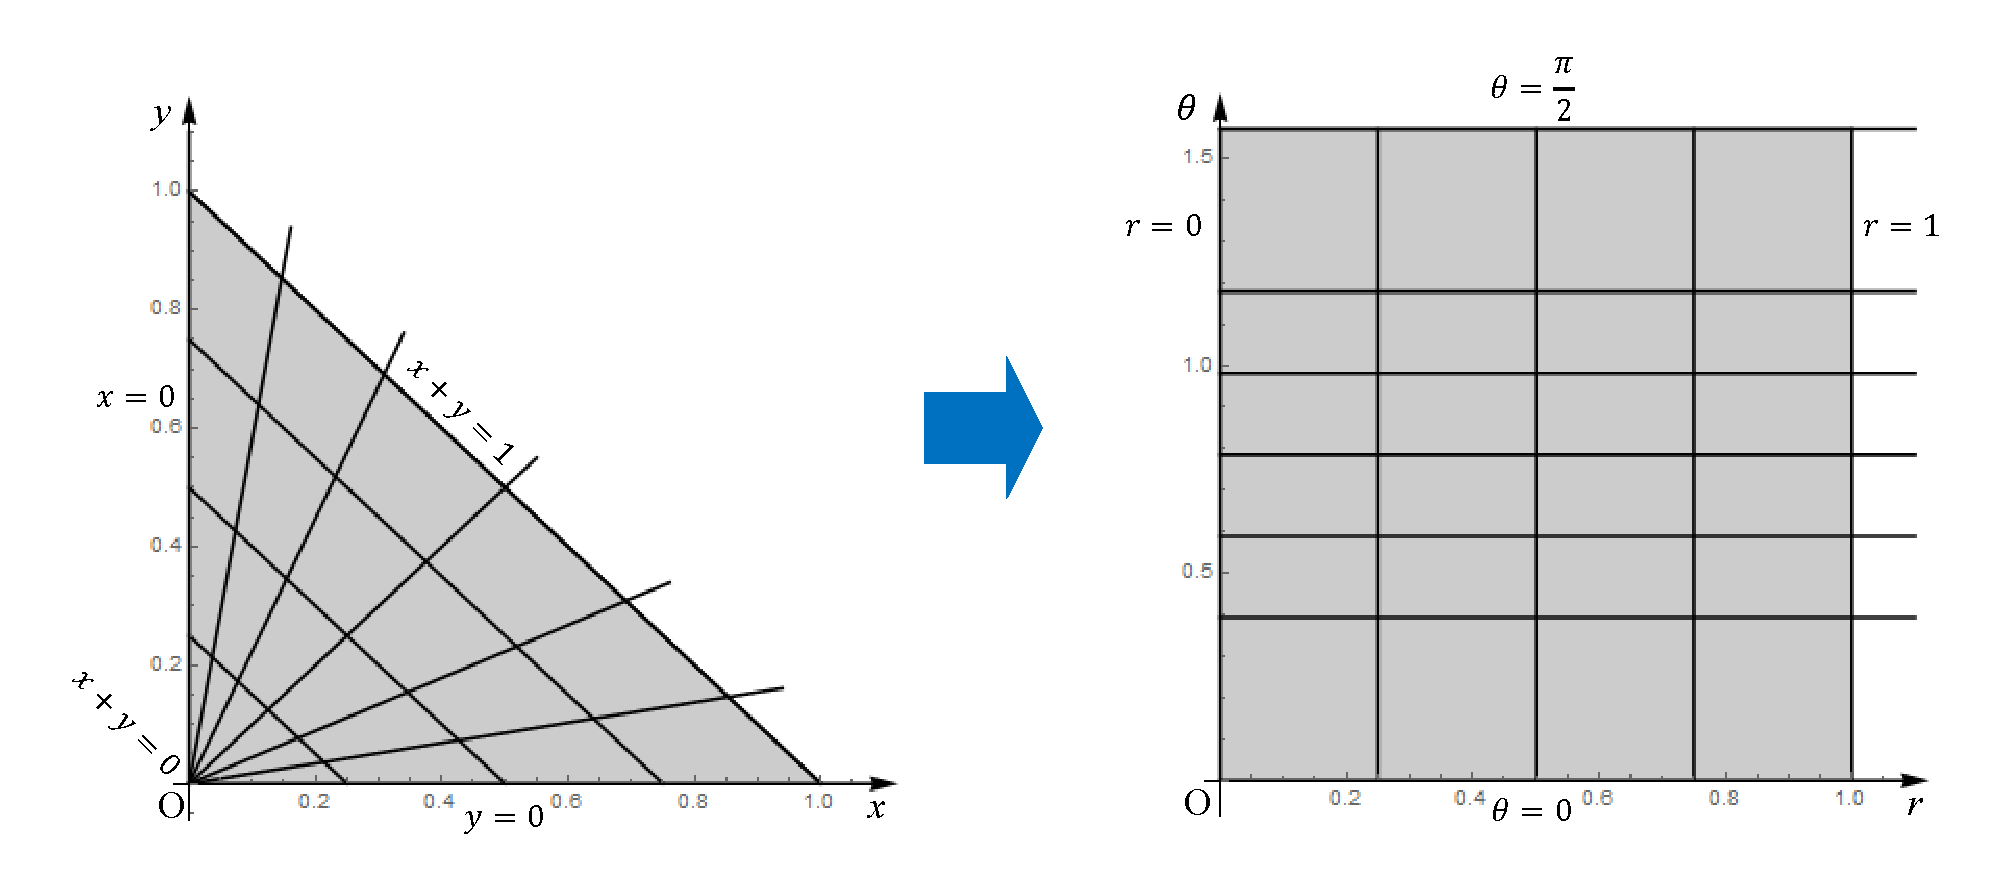
\includegraphics[height=0.3\textheight]{Figures/Fig12-3-2-2.pdf}
\end{center}
\caption{习题12.3 2题方法2图示}
\label{12-3-2-2}
\end{figure}

方法3:令$\begin{cases}
u=x-y,\\
v=x+y,
\end{cases}$则令$\begin{cases}
x=\frac12(u+v),\\
y=\frac12(v-u),
\end{cases}$区域$D=\Set{(u,v)}{0\leqslant v\leqslant1,-v\leqslant u\leqslant v}$,

$\frac{\mathrm D(x,y)}{\mathrm D(u,v)}=\begin{vmatrix}
\frac12&\frac12\\
-\frac12&\frac12
\end{vmatrix}=\frac12$,

$\therefore I=\varIInt D{\cos(\frac uv)|\frac{\mathrm D(x,y)}{\mathrm D(u,v)}|}uv=\frac12\varIInt D{\cos(\frac uv)}uv=\frac12\Int01{}v\Int{-v}v{\cos(\frac uv)}u=\frac12\Int01{}v\Int{-v}v{v\cos(\frac uv)}{\frac uv}\\
=\frac12\Int01{}v[v\sin(\frac uv)]_{-v}^v=\frac12\Int01{[v\sin1-v\sin(-1)]}v=\sin1\Int01vv=\frac12\sin1$.

注意:因为被积函数是$\cos(\frac uv)$,该函数无关于$v$初等原函数,故这种变量代换的方法应先积$u$后积$v$.

{\bf注}:如图\ref{12-3-2-3}所示.\footnotemark\footnotetext{这是修订版增加的内容.}
\begin{figure}[H]
\begin{center}
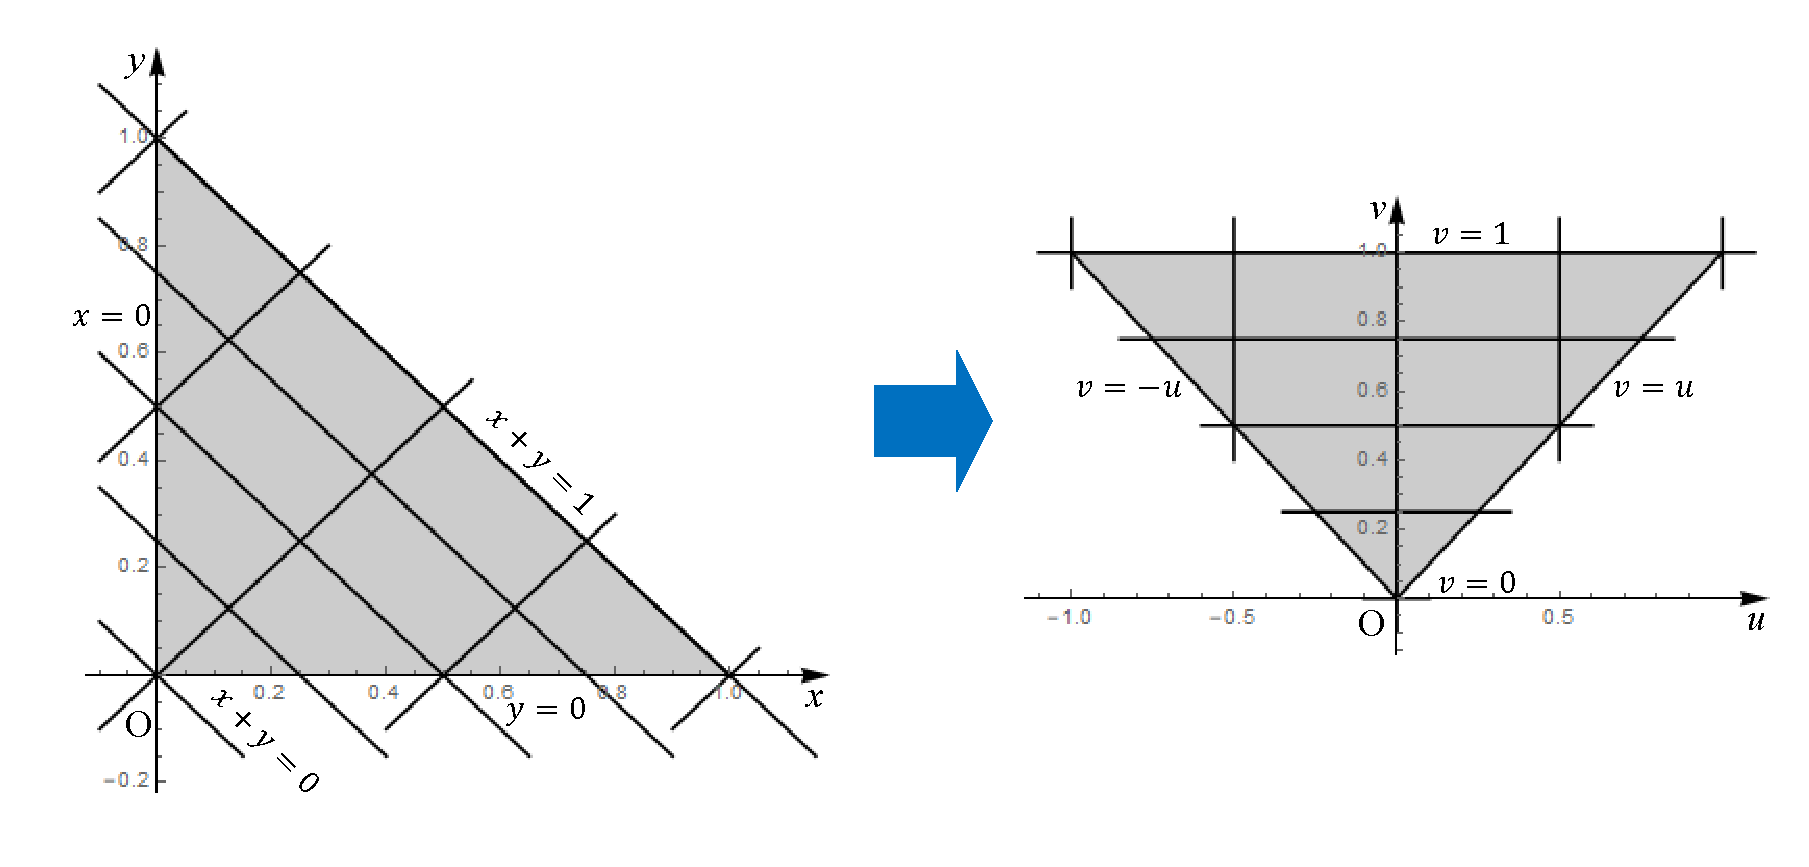
\includegraphics[height=0.3\textheight]{Figures/Fig12-3-2-3.pdf}
\end{center}
\caption{习题12.3 2题方法3图示}
\label{12-3-2-3}
\end{figure}

\item计算$I=\IInt D{(\sqrt x+\sqrt y)}\sigma,D=\Set{(x,y)}{\sqrt x+\sqrt y\leqslant1}$.

解:方法1:令$\begin{cases}
x=r^2\cos^4\theta,\\
y=r^2\sin^4\theta,
\end{cases}$则区域$D=\Set{(r,\theta)}{0\leqslant r\leqslant1,0\leqslant\theta\leqslant\frac\pi2}$,

$\frac{\mathrm D(x,y)}{\mathrm D(r,\theta)}=\begin{vmatrix}
2r\cos^4\theta&-4r^2\cos^3\theta\sin\theta\\
2r\sin^4\theta&4r^2\sin^3\theta\cos\theta
\end{vmatrix}=8r^3\sin^3\theta\cos^3\theta$,

$\therefore I=\IInt D{(\sqrt x+\sqrt y)}\sigma=\varIInt D{r|\frac{\mathrm D(x,y)}{\mathrm D(r,\theta)}|}uv=\varIInt D{8r^4\sin^3\theta\cos^3\theta}uv=\Int01{r^4}r\Int0{\frac\pi2}{2^3\sin^3\theta\cos^3\theta}\theta\\
=\frac15r^5\big|_0^1\frac12\Int0{\frac\pi2}{\sin^32\theta}{2\theta}=\frac1{10}\Int0{\frac\pi2}{\sin^32\theta}{2\theta}=\frac1{10}\Int0\pi{\sin^3\varphi}\varphi=\frac2{10}\Int0{\frac\pi2}{\sin^3\varphi}\varphi=\frac15\frac{2}{3}=\frac2{15}$.

方法2\footnotemark\footnotetext{这是修订版增加的内容.}:令$\begin{cases}
u=\sqrt x,\\
v=\sqrt y,
\end{cases}$则$\begin{cases}
x=u^2,\\
y=v^2,
\end{cases}$区域$D=\Set{(u,v)}{0\leqslant u\leqslant1,0\leqslant v\leqslant1-u}$,

$\frac{\mathrm D(x,y)}{\mathrm D(u,v)}=\begin{vmatrix}
2u&0\\
0&2v
\end{vmatrix}=4uv$,

$\therefore I=\IInt D{(\sqrt x+\sqrt y)}\sigma=\varIInt D{(u+v)|\frac{\mathrm D(x,y)}{\mathrm D(u,v)}|}uv=\varIInt D{(u+v)4uv}uv\\
=4\Int01{}u\Int0{1-u}{(u^2v+uv^2)}v=4\Int01{(\frac12u^2v^2+\frac13uv^3)\big|_0^{1-u}}u\\
=4\Int01{[\frac12u^2(1-u)^2+\frac13u(1-u)^3]}u=4\Int01{(\frac12u^2-u^3+\frac12u^4+\frac13u-u^2+u^3-\frac13u^4)}u\\
=4\Int01{(-\frac12u^2+\frac16u^4+\frac13u)}u=4(-\frac16u^3+\frac1{30}u^5+\frac16u^2)\big|_0^1=\frac2{15}$.

\item在第1象限中,设$D$由$xy=1,xy=2,\frac yx=1$及$\frac yx=4$围成,试证:
\[
\IInt D{f(xy)}\sigma=\ln2\Int12{f(x)}x.
\]
证明:令$\begin{cases}
u=xy,\\
v=\frac yx,
\end{cases}$则区域$D=\Set{(u,v)}{1\leqslant u\leqslant2,1\leqslant v\leqslant4}$,

$\frac{\mathrm D(u,v)}{\mathrm D(x,y)}=\begin{vmatrix}
y&x\\
-\frac y{x^2}&\frac1x
\end{vmatrix}=\frac yx+\frac yx=2v,\ |\frac{\mathrm D(x,y)}{\mathrm D(u,v)}|=\frac1{2v}$,

$\therefore\IInt D{f(xy)}\sigma=\varIInt D{f(u)|\frac{\mathrm D(x,y)}{\mathrm D(u,v)}|}uv=\Int12{f(u)}u\Int14{\frac1{2v}}v=\frac12\ln v\big|_1^4\Int12{f(u)}u\\
=2\ln2\Int12{f(u)}u=\ln2\Int12{f(x)}x.$
\end{enumerate}
\end{document}
\documentclass[12pt,UTF8]{ctexart}
\usepackage{ctex,amsmath,amssymb,geometry,fancyhdr,bm,amsfonts,mathtools,extarrows,graphicx,url,enumerate,color,float,multicol,subfigure,wasysym} 
\allowdisplaybreaks[4]
% 加入中文支持
\newcommand\Set[2]{\left\{#1\ \middle\vert\ #2 \right\}}
\newcommand\Lim[0]{\lim\limits_{n\rightarrow\infty}}
\newcommand\LIM[2]{\lim\limits_{#1\rightarrow#2}}
\newcommand\Ser[1]{\sum_{n=#1}^\infty}
\newcommand{\SER}[2]{\sum_{#1=#2}^\infty}
\newcommand{\Int}[4]{\varint\nolimits_{#1}^{#2}#3\mathrm d#4}
\newcommand{\aIInt}[1]{\iint\limits_{#1}}
\newcommand{\IInt}[3]{\iint\limits_{#1}#2\mathrm d#3}
\newcommand{\varIInt}[4]{\iint\limits_{#1}#2\mathrm d#3\mathrm d#4}
\newcommand{\IIInt}[3]{\iiint\limits_{#1}#2\mathrm d#3}
\newcommand{\varIIInt}[5]{\iiint\limits_{#1}#2\mathrm d#3\mathrm d#4\mathrm d#5}
\geometry{a4paper,scale=0.80}
\pagestyle{fancy}
\rhead{习题12.4}
\lhead{基础习题课讲义}
\chead{微积分B(2)}
\begin{document}
\setcounter{section}{18}
\section{三重积分的计算}
\subsection{知识结构}
\noindent第12章重积分
	\begin{enumerate}
		\item[12.4]三重积分的计算
			\begin{enumerate}
				\item[12.4.1]三重积分在直角坐标系下的计算
				\item[12.4.2]三重积分的变量代换
				\item[12.4.3]用柱坐标计算三重积分
				\item[12.4.4]用球坐标计算三重积分
			\end{enumerate}
	\end{enumerate}
\subsection{习题12.4解答}
\begin{enumerate}
\item求$I=\Int01{}x\Int0x{}y\Int0y{\frac{\sin z}{(1-z)^2}}z$的值.

\begin{figure}[H]
\begin{center}
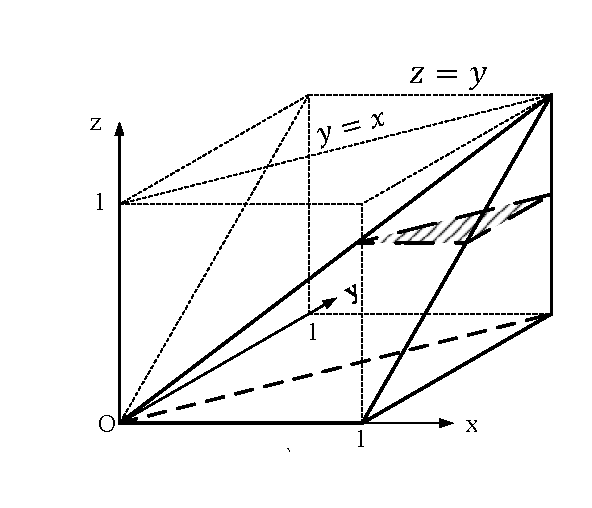
\includegraphics[height=0.4\textheight]{Figures19/Fig12-4-1.pdf}
\end{center}
\caption{习题12.4 1.题图示}
\label{12-4-1}
\end{figure}

解:$I=\Int01{}x\Int0x{}y\Int0y{\frac{\sin z}{(1-z)^2}}z=\Int01{\frac{\sin z}{(1-z)^2}}z\Int z1{}y\Int y1{}x=\Int01{\frac{\sin z}{(1-z)^2}}z\Int z1{(1-y)}y\\
=\Int01{\frac{\sin z}{(1-z)^2}(y-\frac12 y^2)\big|_z^1}z=\Int01{\frac{\sin z}{(1-z)^2}(\frac12-z+\frac12z^2)}z=\frac12\Int01{\frac{\sin z}{(1-z)^2}(1-z)^2}z\\
=\frac12\Int01{\sin z}z=\frac12(-\cos z)\big|_0^1=\frac12(1-\cos1)$.

\item用直角坐标计算三重积分$\varIIInt{\Omega}zxyz$,其中$\Omega$由曲面$x^2+y^2-2z^2=1$,平面$z=1$及$z=2$围成.

\begin{figure}[H]
\begin{center}
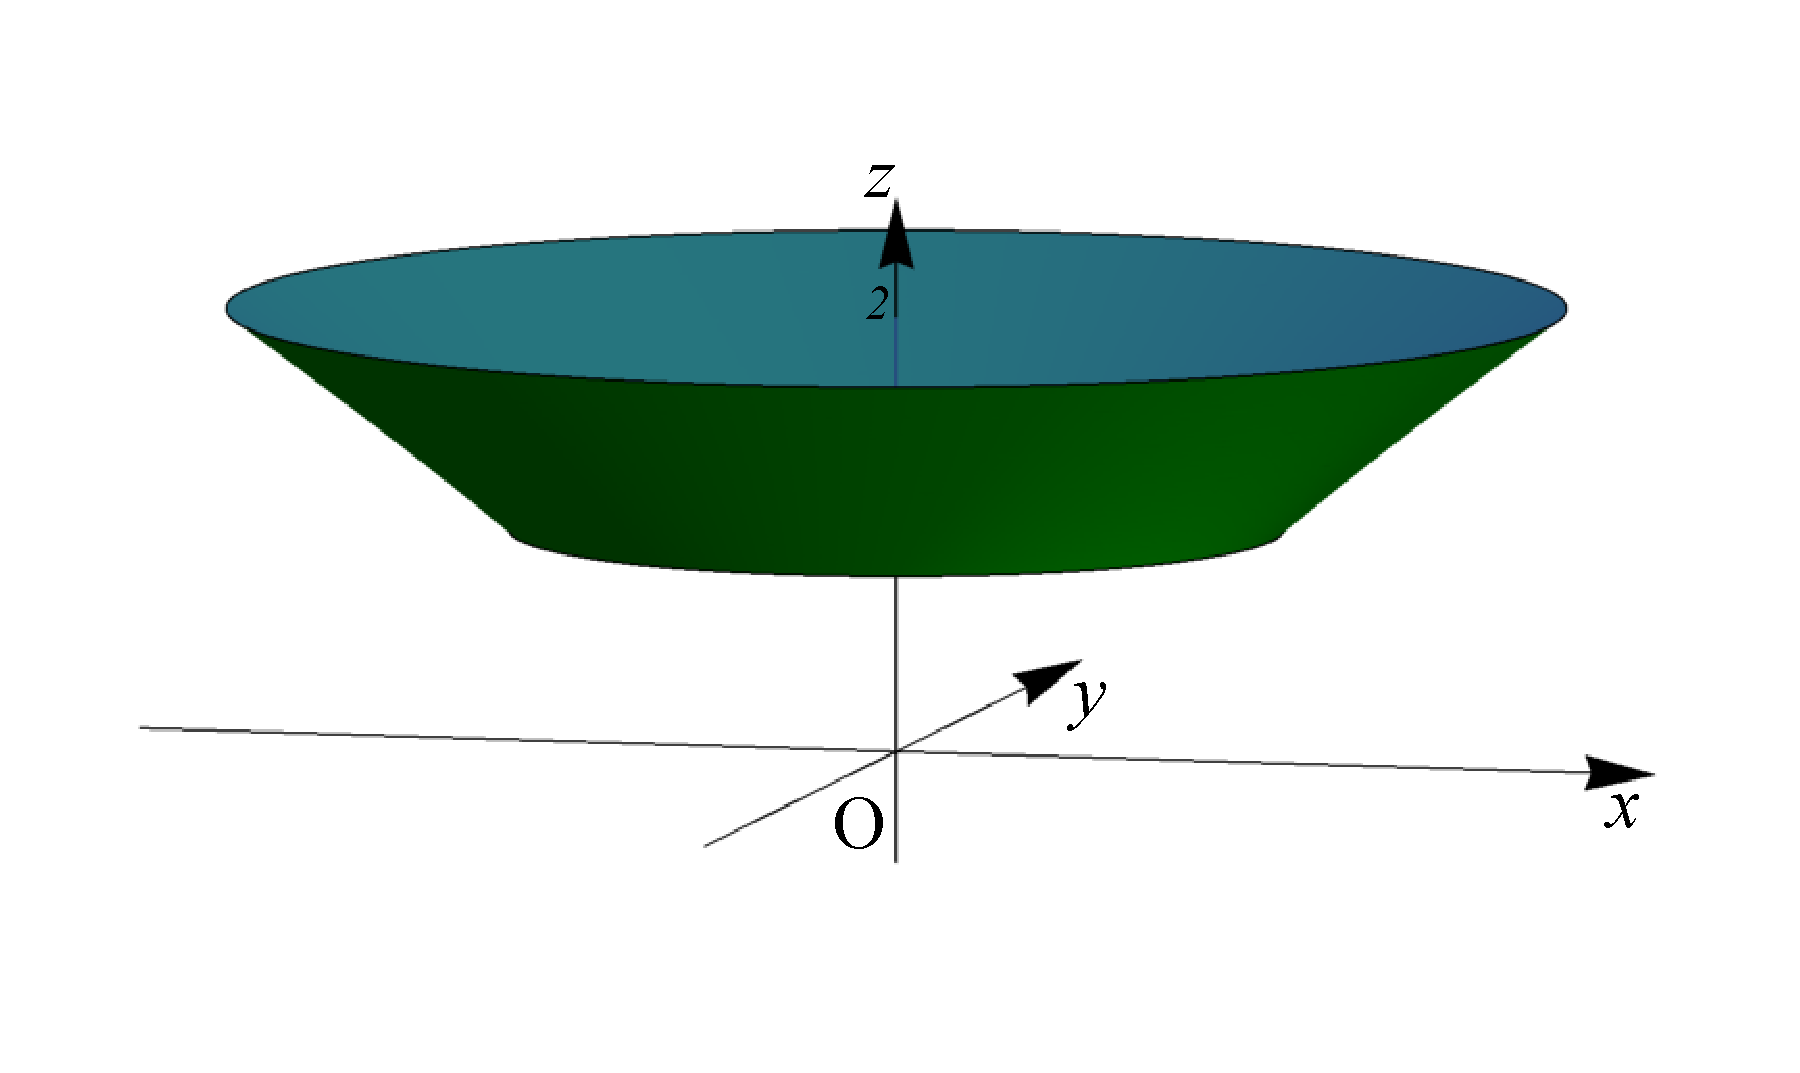
\includegraphics[height=0.4\textheight]{Figures19/Fig12-4-2.pdf}
\end{center}
\caption{习题12.4 2.题图示}
\label{12-4-2}
\end{figure}

解:$\varIIInt{\Omega}zxyz=\Int12zz\varIInt{\Omega_z}{}xy=\Int12{z\pi(1+2z^2)}z=\pi(\frac12z^2+\frac12z^4)\big|_1^2=9\pi$.

\item用柱面坐标计算三重积分$\varIIInt\Omega{\sqrt{y^2+z^2}}xyz$,其中$\Omega$为$y^2+z^2\leqslant x^2,1\leqslant x\leqslant2$.

\begin{figure}[H]
\begin{center}
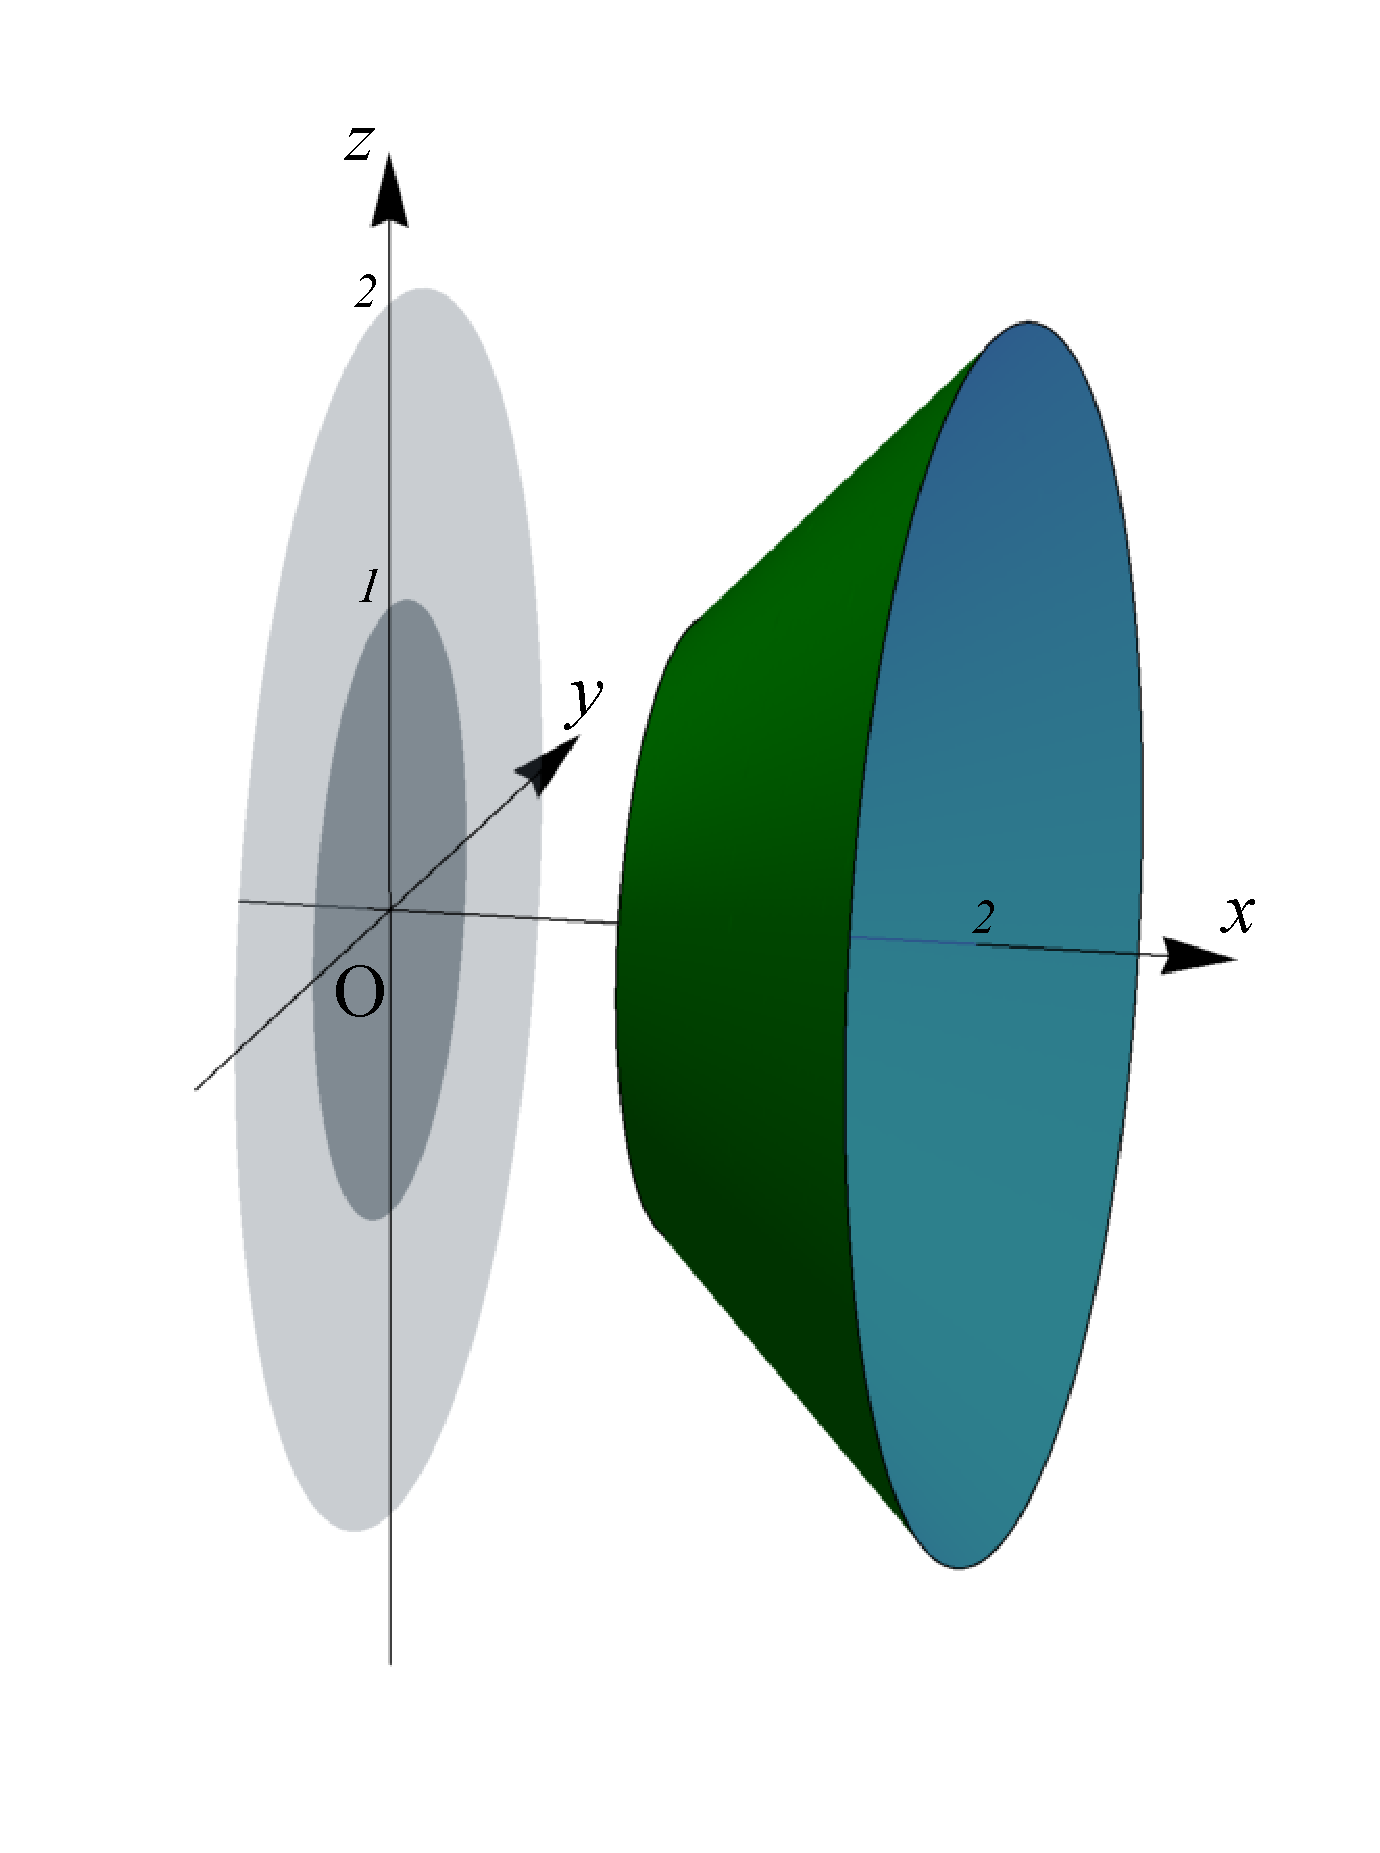
\includegraphics[height=0.4\textheight]{Figures19/Fig12-4-3.pdf}
\end{center}
\caption{习题12.4 3.题图示}
\label{12-4-3}
\end{figure}

解:$\because\Omega=\Set{(x,y)}{y^2+z^2\leqslant x^2,1\leqslant x\leqslant2}=\Set{(x,y)}{y^2+z^2\leqslant1,1\leqslant x\leqslant2}\cup\\
\Set{(x,y)}{1\leqslant y^2+z^2\leqslant x^2,1\leqslant x\leqslant2}=\Omega_1\cup\Omega_2$,

$\therefore\varIIInt\Omega{\sqrt{y^2+z^2}}xyz=\varIIInt{\Omega_1}{\sqrt{y^2+z^2}}xyz+\varIIInt{\Omega_2}{\sqrt{y^2+z^2}}xyz\\
=\Int0{2\pi}{}\theta\Int01{}r\Int12{r\cdot r}x+\Int0{2\pi}{}\theta\Int12{}r\Int r2{r\cdot r}x=2\pi\Int01{r^2}r+2\pi\Int12{r^2(2-r)}r\\
=2\pi\frac13r^3\big|_0^1+2\pi(\frac23r^3-\frac14r^4)\big|_1^2=\frac52\pi$.

\item(1)用球面坐标计算三重积分$\varIIInt\Omega zxyz$,其中$\Omega$由曲面$z=\sqrt{a^2-x^2-y^2}$及$z=\sqrt{x^2+y^2}$围成;\\
(2)设$\Omega$是由曲面$z=\sqrt{x^2+y^2}$与$z=\sqrt{1-x^2-y^2}$围成的空间区域,求$\IIInt\Omega{(x+z)}V$.

\begin{figure}[H]
\begin{center}
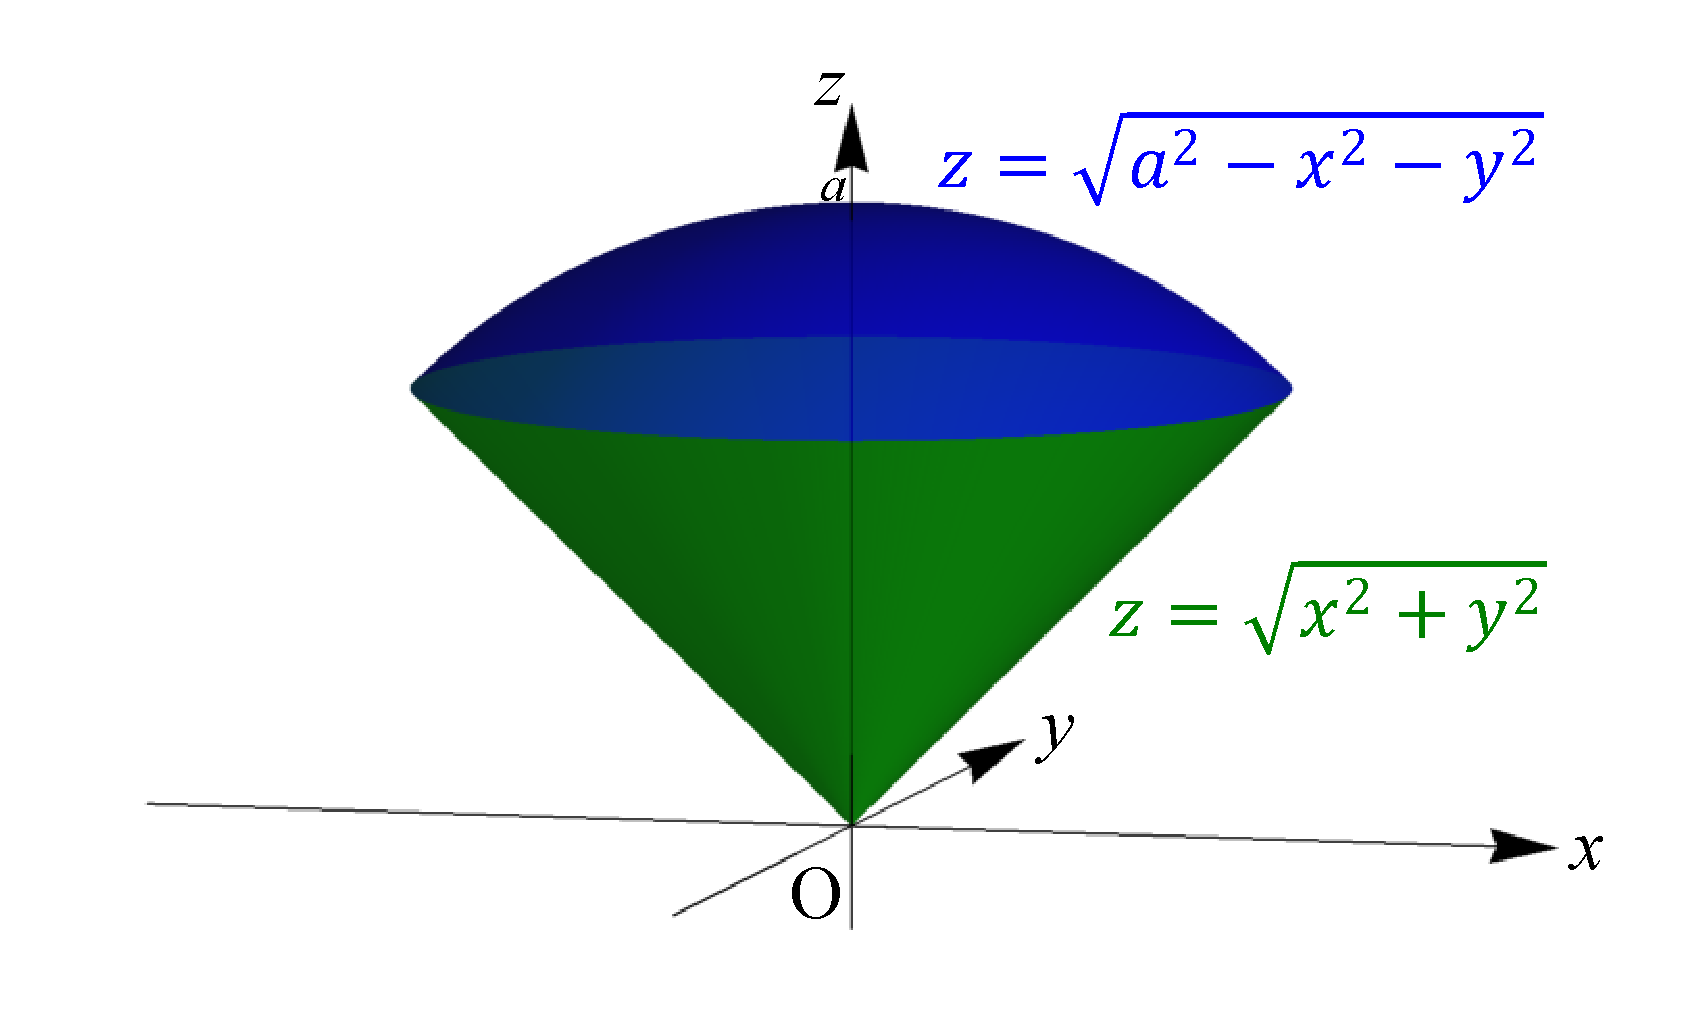
\includegraphics[height=0.4\textheight]{Figures19/Fig12-4-4-1.pdf}
\end{center}
\caption{习题12.4 4.(1)题图示}
\label{12-4-4-1}
\end{figure}

解:(1)$\because$曲面$z=\sqrt{a^2-x^2-y^2}$和$z=\sqrt{x^2+y^2}$的交线所在的投影柱面为$x^2+y^2=\frac{a^2}2$,

$\therefore$交线对应的极角正弦$\sin\varphi_0=\frac{\frac a{\sqrt2}}{a}=\frac1{\sqrt2}$,

$\therefore\varphi_0=\frac\pi4$,

$\therefore\varIIInt\Omega zxyz=\Int0{\frac\pi4}{}\varphi\Int0{2\pi}{}\theta\Int0a{r\cos\varphi r^2\sin\varphi}r=2\pi\Int0{\frac\pi4}{\sin\varphi\cos\varphi}\varphi\Int0a{r^3}r\\
=2\pi\cdot\frac12\sin^2\varphi\big|_0^{\frac\pi4}\cdot\frac14r^4\big|_0^a=\frac\pi8a^4$.

(2)由对称性可知$\IIInt\Omega{x}V=0$,

$\therefore\IIInt\Omega{(x+z)}V=\varIIInt\Omega{z}xyz=\frac\pi8$.

\item设$\Omega$是由曲线$\begin{cases}
x=0,\\
y^2=2z,
\end{cases}$绕$z$轴旋转一周而成的曲面与平面$z=4$围成的空间区域,求$\IIInt\Omega{(x^2+y^2+z)}V$.

\begin{figure}[H]
\begin{center}
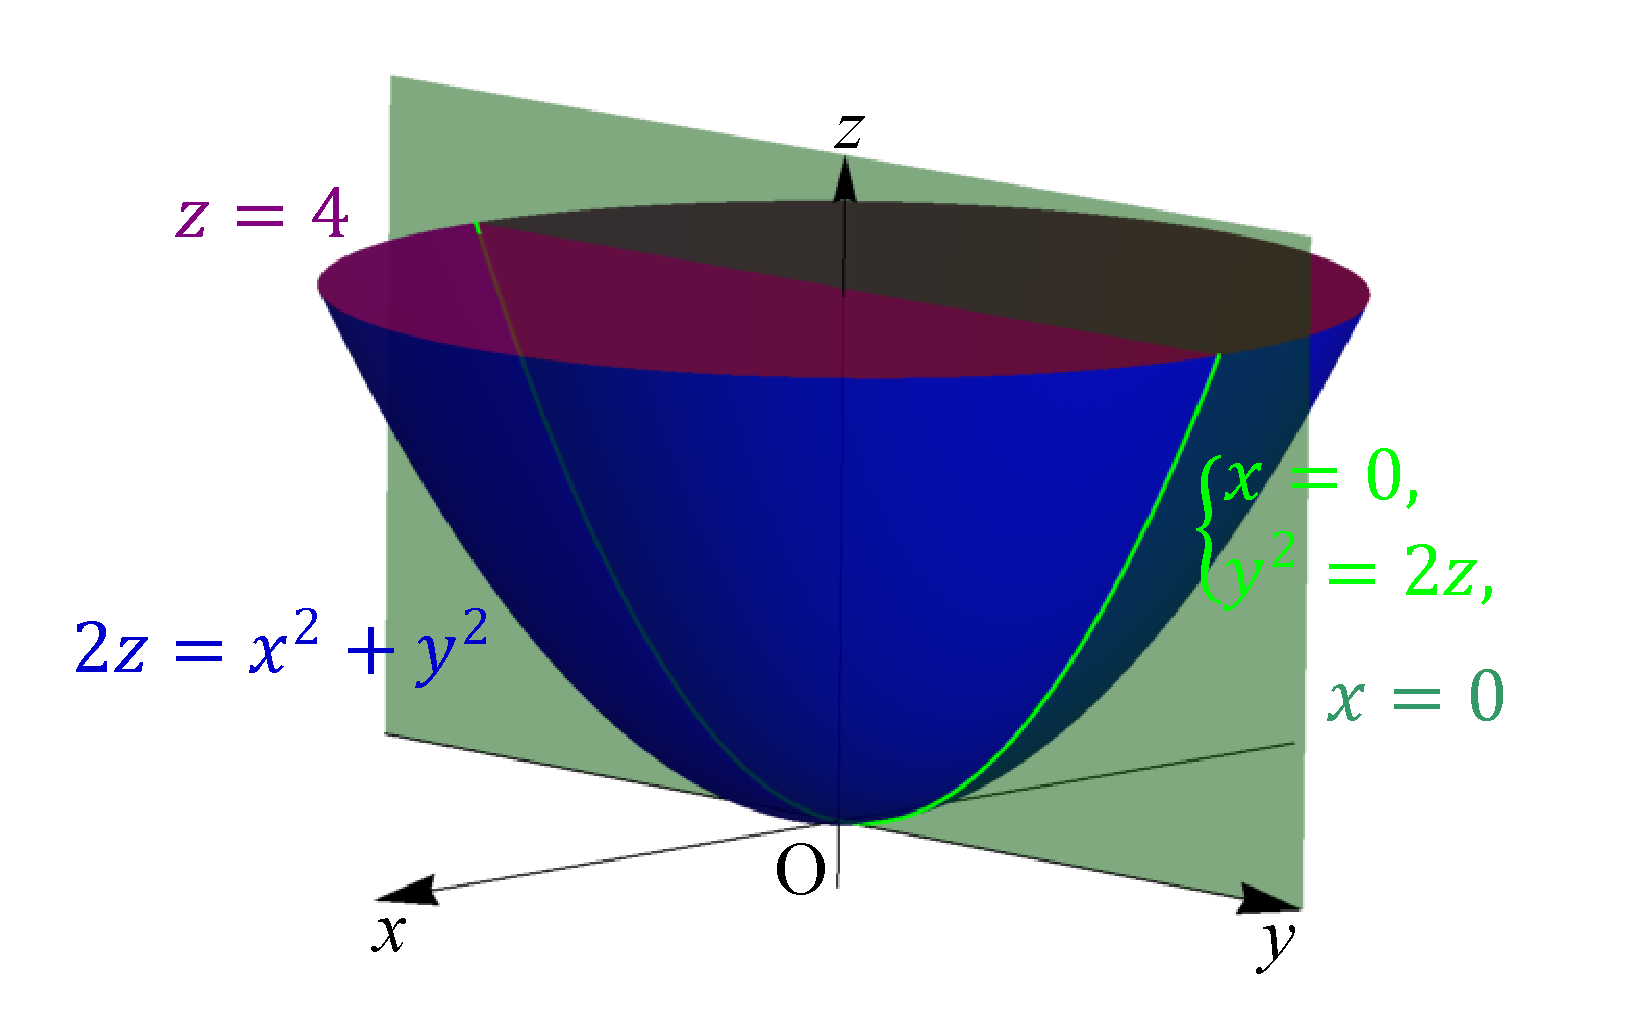
\includegraphics[height=0.4\textheight]{Figures19/Fig12-4-5.pdf}
\end{center}
\caption{习题12.4 5.题图示}
\label{12-4-5}
\end{figure}

解:$\Omega=\Set{(x,y)}{x^2+y^2\leqslant2z,0\leqslant z\leqslant4}$,

$\therefore\IIInt\Omega{(x^2+y^2+z)}V=\Int0{2\pi}{}\theta\Int0{2\sqrt2}{}r\Int{\frac12r^2}4{(r^2+z)r}z=2\pi\Int0{2\sqrt2}{(r^3z+\frac12rz^2)_{\frac12r^2}^4}r\\
=2\pi\Int0{2\sqrt2}{(4r^3+8r-\frac12r^5-\frac18r^5)}r=2\pi(r^4+4r^2-\frac58\cdot\frac16r^6)\big|_0^{2\sqrt2}=\frac{256}3\pi$.

\item在直角坐标、柱坐标和球坐标系下将积分$I=\IIInt\Omega{z^2}V$化为累次积分,并选择其中一种坐标计算,其中$\Omega=\Set{(x,y,z)}{x^2+y^2+z^2\leqslant R^2,x^2+y^2+(z-R)^2\leqslant R^2}$.

\begin{figure}[H]
\begin{center}
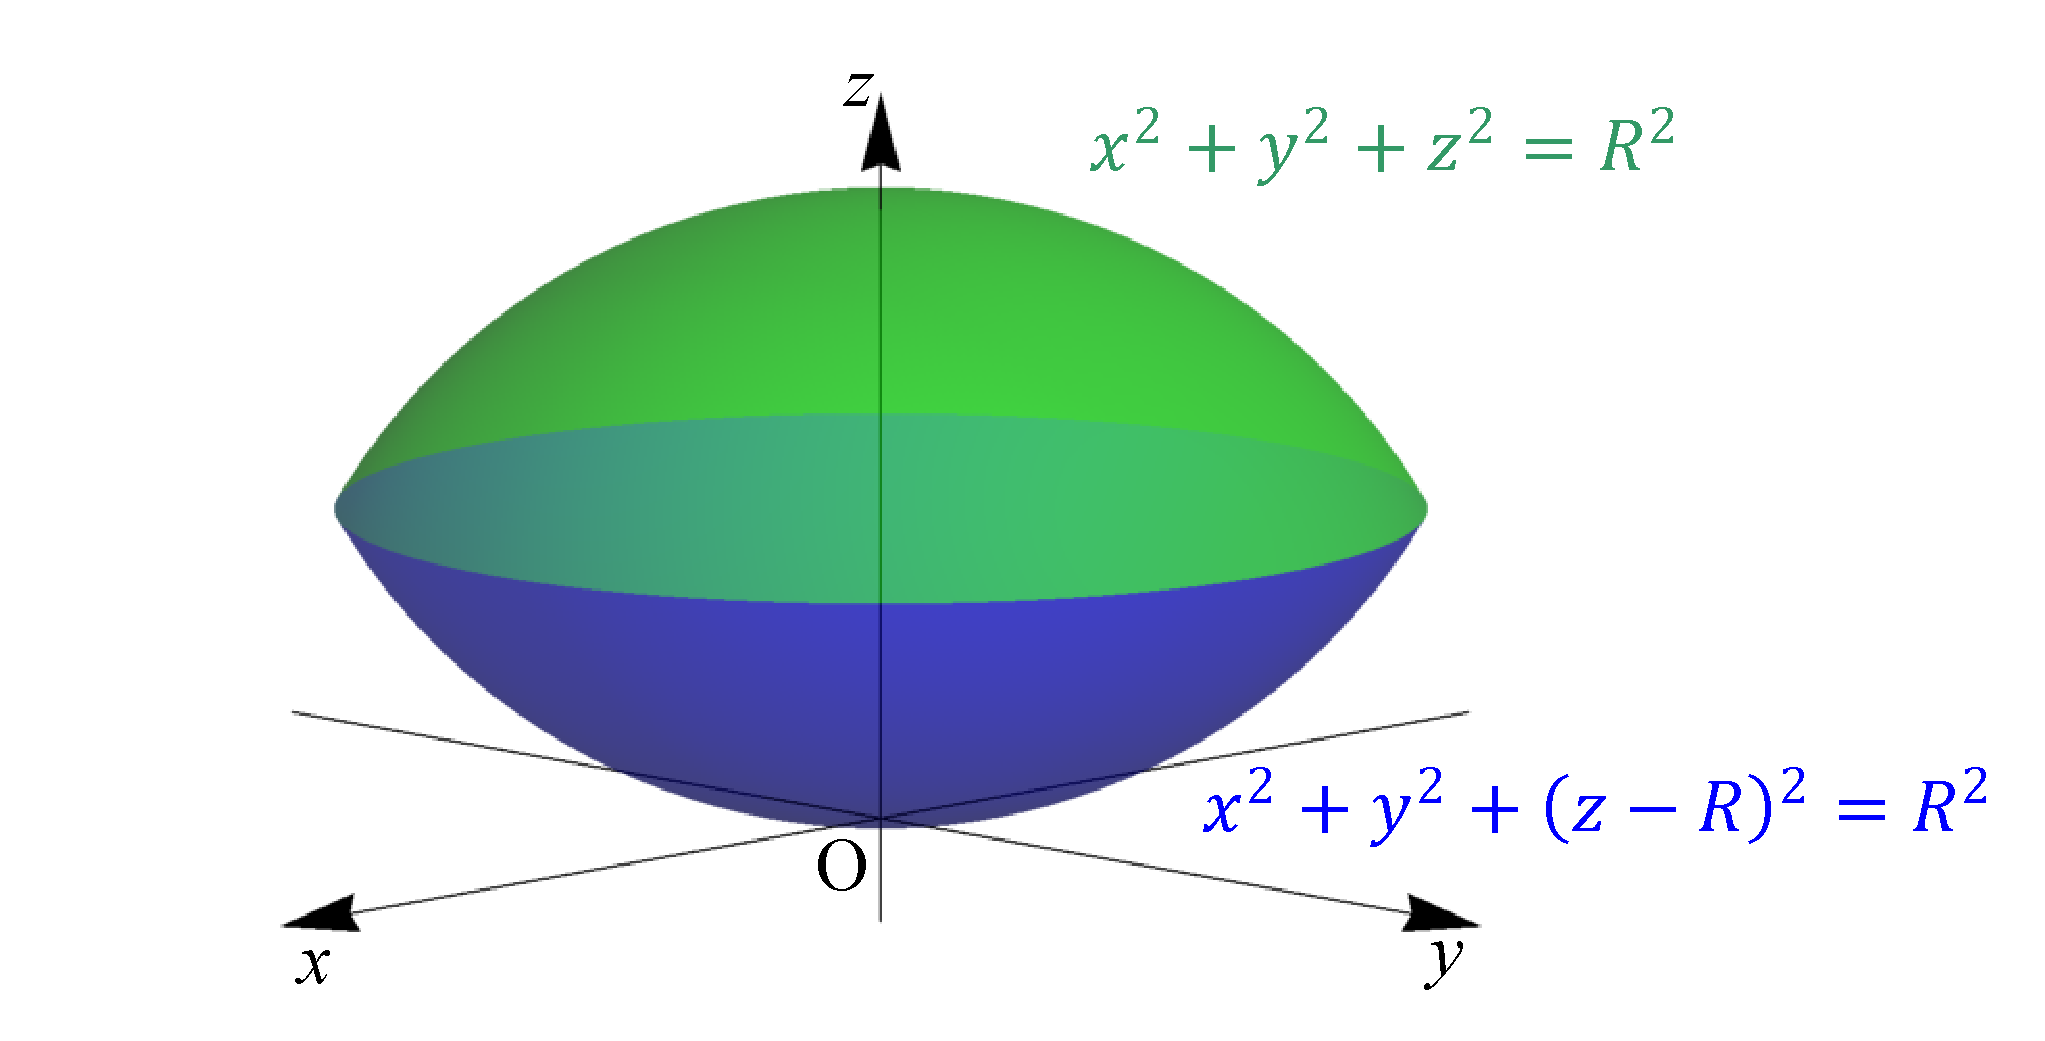
\includegraphics[height=0.4\textheight]{Figures19/Fig12-4-6-1.pdf}
\end{center}
\caption{习题12.4 6.题积分域}
\label{12-4-6}
\end{figure}

解:由$\begin{cases}
x^2+y^2+z^2=R^2,\\
x^2+y^2+(z-R)^2=R^2,
\end{cases}$得交线$\begin{cases}
z=\frac R2,\\
x^2+y^2=\frac34R^2,
\end{cases}$\\
交线对应的极角的正弦$\sin\varphi_0=\frac{\sqrt3}2$,则$\varphi_0=\frac\pi3$.

在直角坐标系下:

\begin{figure}[H]
\begin{center}
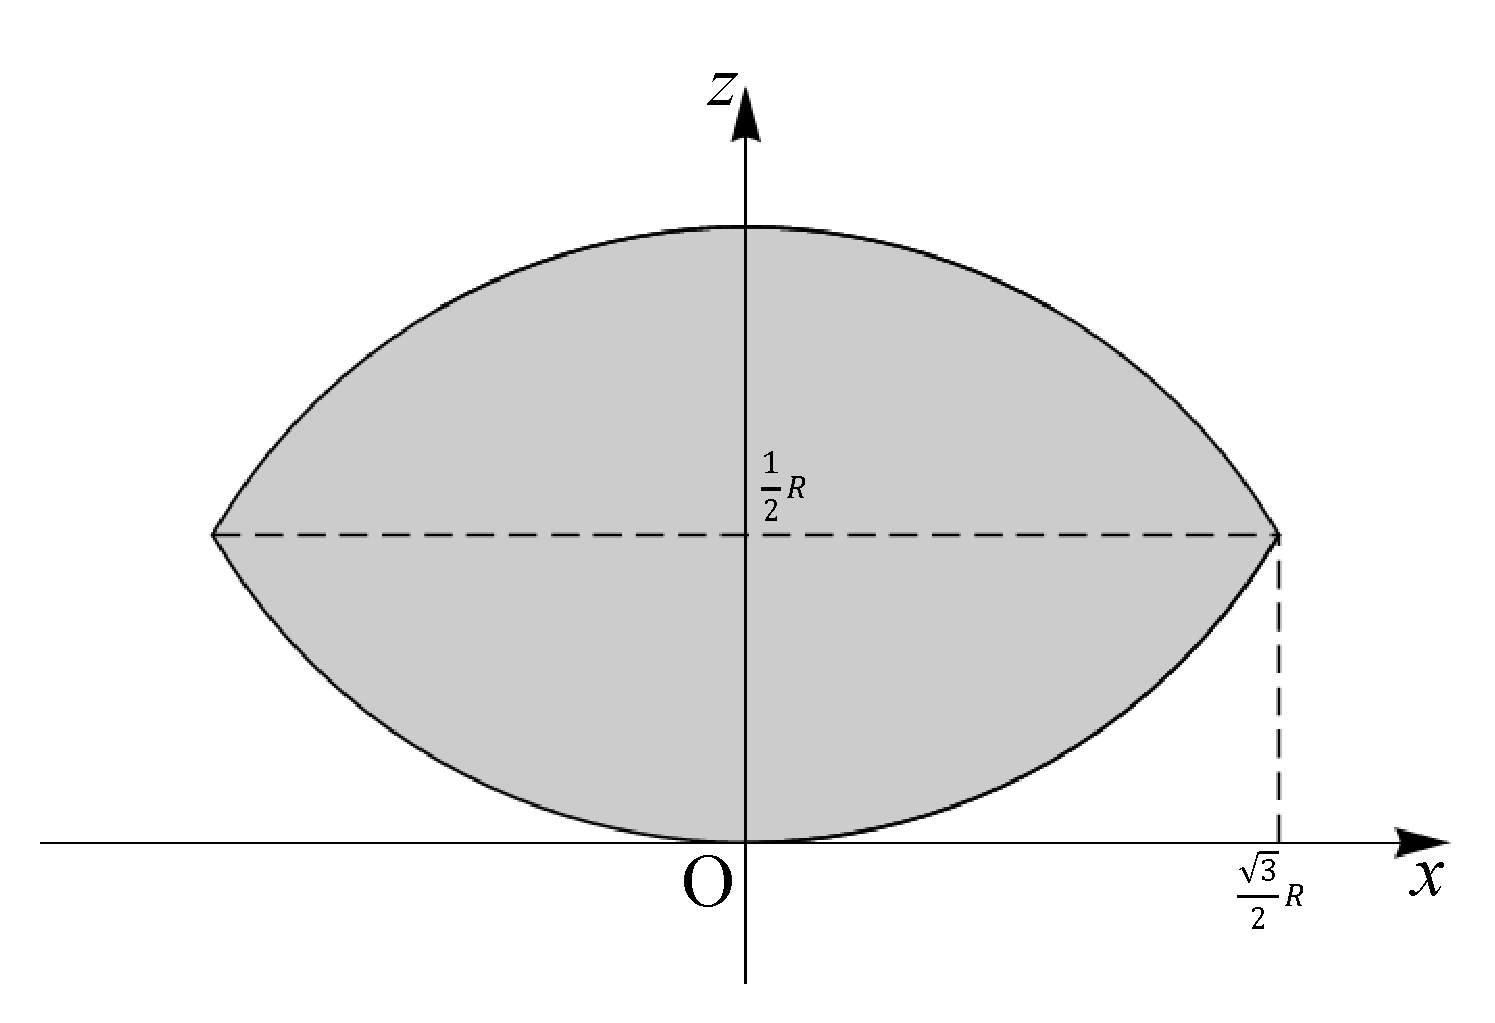
\includegraphics[height=0.4\textheight]{Figures19/Fig12-4-6-2.pdf}
\end{center}
\caption{习题12.4 6.题积分域在$xOz$坐标面上的截面图形(直角坐标系)}
\label{12-4-6-2}
\end{figure}

$I=\IIInt\Omega{z^2}V=\Int0{\frac R2}{z^2}z\varIInt{\Omega_z}{}xy+\Int{\frac R2}R{z^2}z\varIInt{\Omega_z}{}xy\\
=\Int0{\frac R2}{z^2\pi[R^2-(z-R)^2]}z+\Int{\frac R2}R{z^2\pi(R^2-z^2)}z\\
=\pi\Int0{\frac R2}{(2Rz^3-z^4)}z+\pi\Int{\frac R2}R{(R^2z^2-z^4)}z\\
=\pi(\frac12Rz^4-\frac15z^5)\big|_0^{\frac R2}+\pi(\frac13R^2z^3-\frac15z^5)\big|_{\frac R2}^R=\frac{59}{480}\pi R^5$.

或者:

$I=\IIInt\Omega{z^2}V=\Int{-\frac{\sqrt3}2R}{\frac{\sqrt3}2R}{}x\Int{-\sqrt{\frac34R^2-x^2}}{\sqrt{\frac34R^2-x^2}}{}y\Int{R-\sqrt{R^2-x^2-y^2}}{\sqrt{R^2-x^2-y^2}}{z^2}z$.

在柱坐标系下:

$I=\IIInt\Omega{z^2}V=\Int0{2\pi}{}\theta\Int0{\frac{\sqrt3}2R}{}r\Int{R-\sqrt{R^2-r^2}}{\sqrt{R^2-r^2}}{z^2r}z$.

在球坐标系下:
 
\begin{figure}[H]
\begin{center}
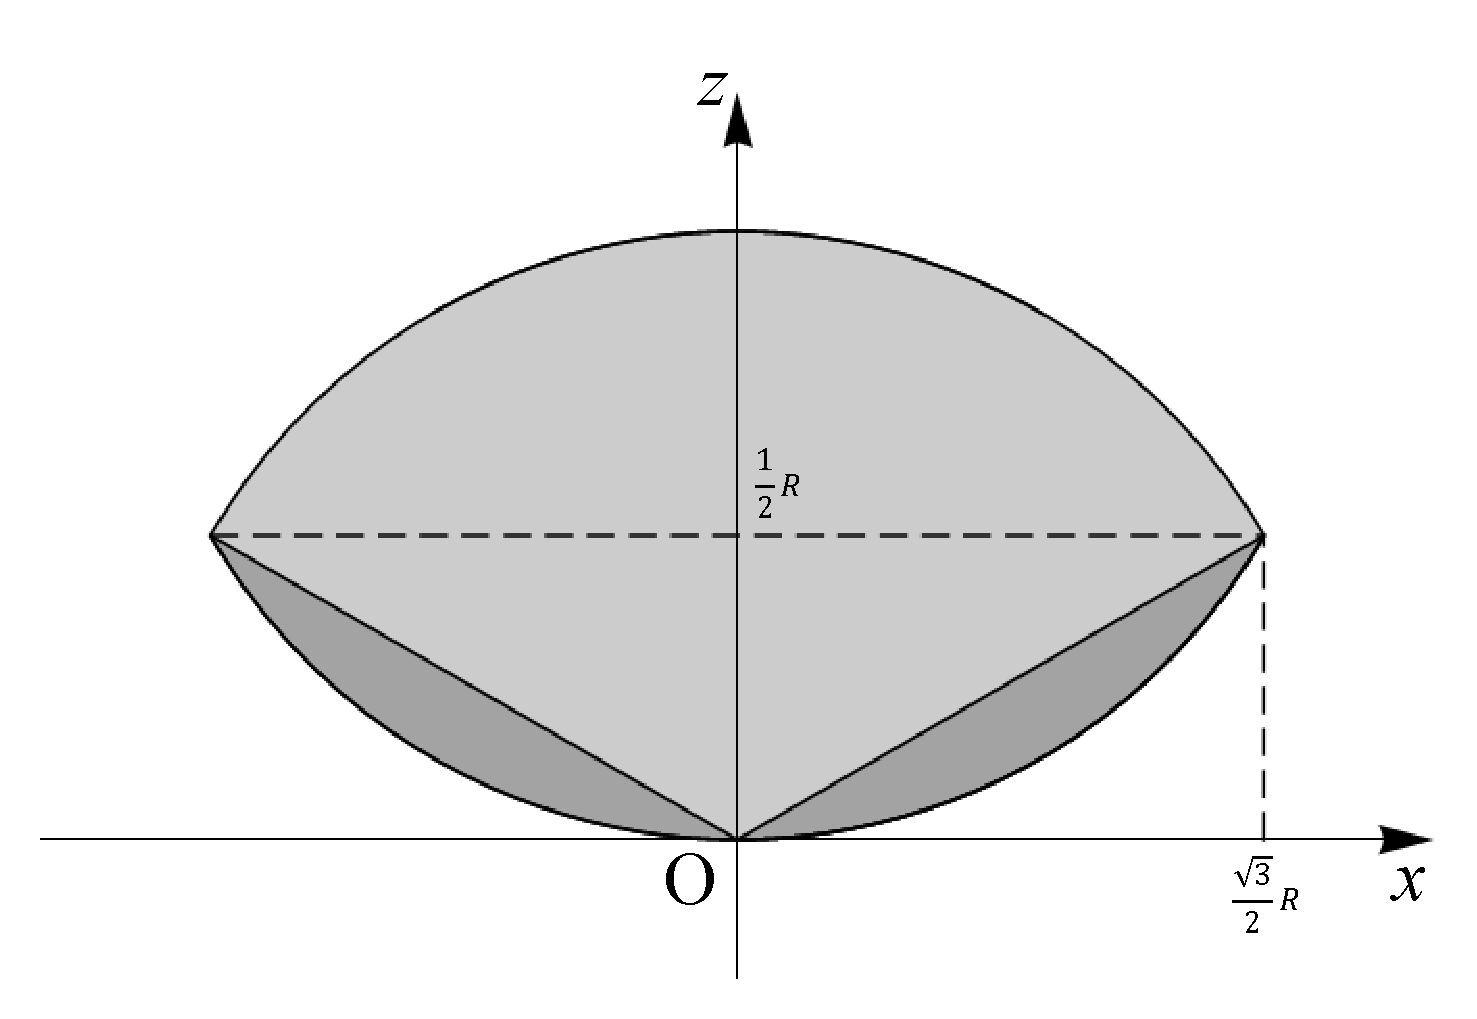
\includegraphics[height=0.4\textheight]{Figures19/Fig12-4-6-3.pdf}
\end{center}
\caption{习题12.4 6.题积分域在$xOz$坐标面上的截面图形(球坐标系)}
\label{12-4-6-3}
\end{figure}

$I=\IIInt\Omega{z^2}V=\Int0{\frac\pi3}{}\varphi\Int0{2\pi}{}\theta\Int0R{r^2\cos^2\varphi r^2\sin\varphi}r+\Int{\frac\pi3}{\frac\pi2}{}\varphi\Int0{2\pi}{}\theta\Int0{2R\cos\varphi}{r^2\cos^2\varphi r^2\sin\varphi}r\\
=2\pi\Int0{\frac\pi3}{\cos^2\varphi\sin\varphi}\varphi\Int0R{r^4}r+2\pi\Int{\frac\pi3}{\frac\pi2}{}\varphi\Int0{2R\cos\varphi}{r^4\cos^2\varphi\sin\varphi}r\\
=2\pi(-\frac13\cos^3\varphi)\big|_0^{\frac\pi3}\frac15r^5\big|_0^R+2\pi\Int{\frac\pi3}{\frac\pi2}{\cos^2\varphi\sin\varphi\frac15r^5\big|_0^{2R\cos\varphi}}\varphi\\
=2\pi(\frac13-\frac13\frac18)\frac15R^5+2\pi\Int{\frac\pi3}{\frac\pi2}{\frac{32}5R^5\cos^7\varphi\sin\varphi}\varphi=2\pi\frac13\cdot\frac78\cdot\frac15-\frac{64\pi}5R^5\frac18\cos^8\varphi\big|_{\frac\pi3}^{\frac\pi2}\\
=\frac{7\pi}{3\times4\times5}-\frac{8\pi}5R^5(0-\frac1{2^8})=\frac{59}{480}\pi R^5$.

\item$\varIIInt\Omega{|z-\sqrt{x^2+y^2}|}xyz$,其中$\Omega$由平面$z=0,z=1$及曲面$x^2+y^2=2$围成.

%\begin{figure}[H]
%\begin{center}
%\subfloat[积分域]{\label{12-4-7-1}
%{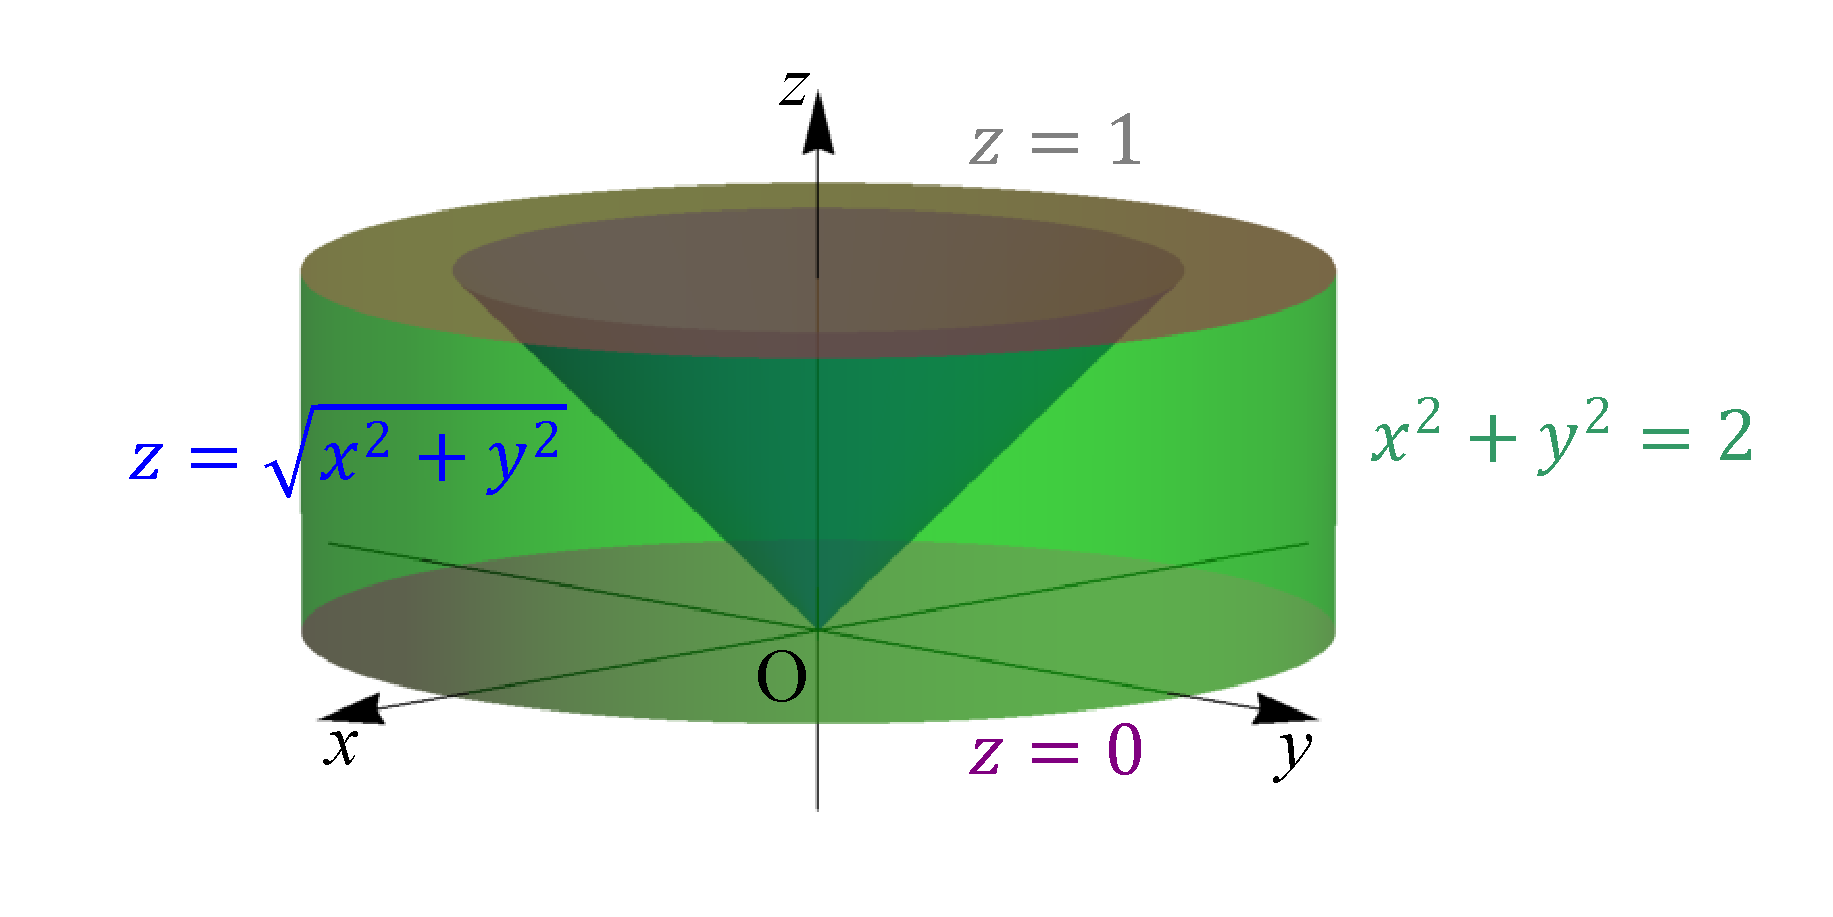
\includegraphics[height=0.3\textheight]{Figures19/Fig12-4-7-1.pdf} }}\\
%\subfloat[积分域在$xOz$坐标面上的截面]{\label{12-4-7-2}
%{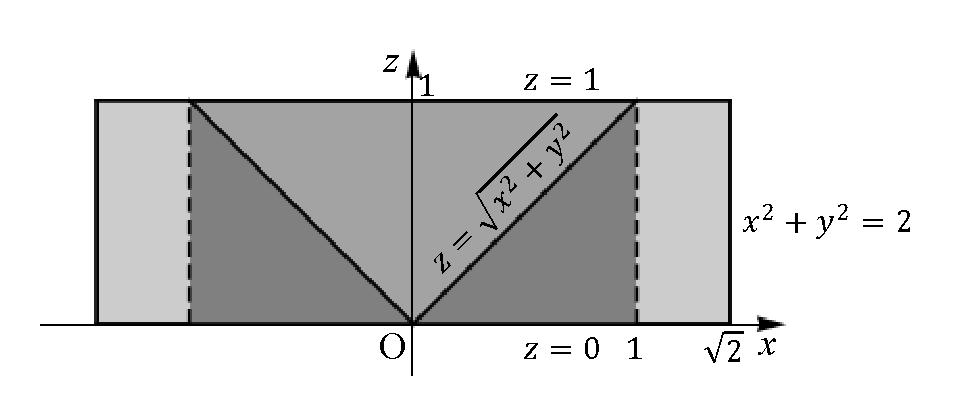
\includegraphics[height=0.3\textheight]{Figures19/Fig12-4-7-2.pdf} }}
%\end{center}
%\caption{习题12.4 7.题图示}
%\label{12-4-7}
%\end{figure}

\begin{figure}[H]
\begin{center}
\subfigure[积分域]{\label{12-4-7-1}
{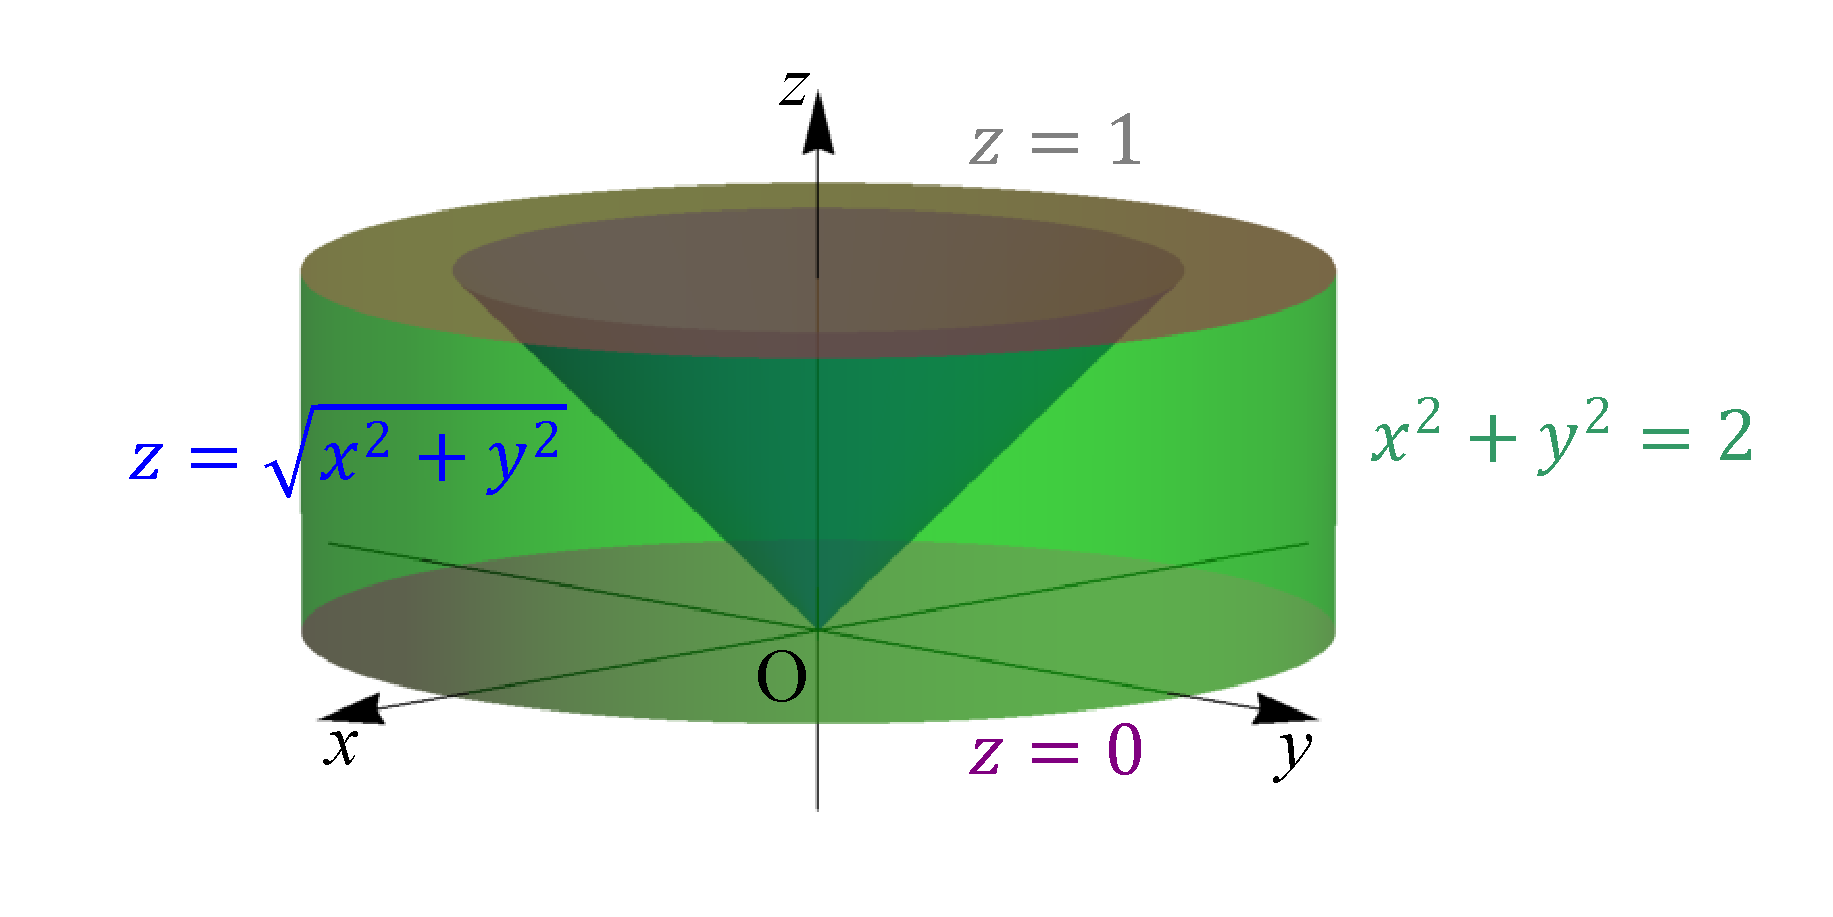
\includegraphics[height=0.3\textheight]{Figures19/Fig12-4-7-1.pdf} }}\\
\subfigure[积分域在$xOz$坐标面上的截面]{\label{12-4-7-2}
{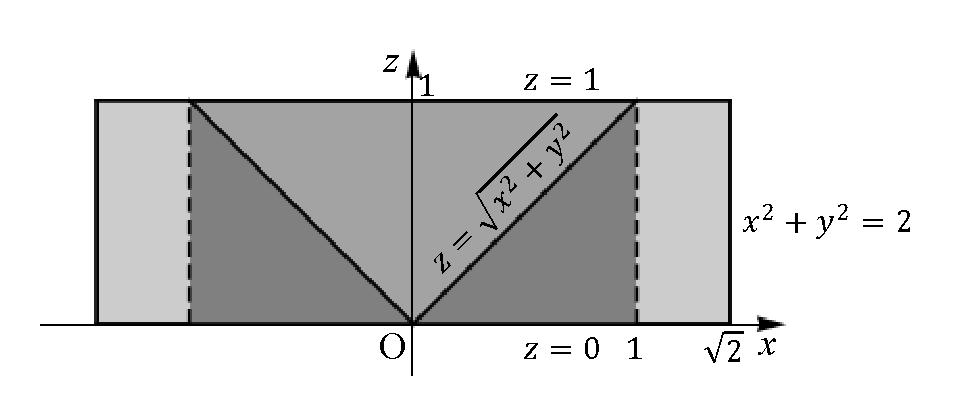
\includegraphics[height=0.3\textheight]{Figures19/Fig12-4-7-2.pdf} }}
\end{center}
\caption{习题12.4 7.题图示}
\label{12-4-7}
\end{figure}

解:$\varIIInt\Omega{|z-\sqrt{x^2+y^2}|}xyz=\Int0{2\pi}{}\theta\Int1{\sqrt2}{}r\Int01{(r-z)r}z+\Int0{2\pi}{}\theta\Int01{}r\Int0{r}{(r-z)r}z+\Int0{2\pi}{}\theta\Int01{}r\Int r1{(z-r)r}z\\
=2\pi\Int1{\sqrt2}{(r^2z-\frac12rz^2)\big|_0^1}r+2\pi\Int01{(r^2z-\frac12rz^2)\big|_0^r}r+2\pi\Int01{(\frac12rz^2-r^2z)\big|_r^1}r\\
=2\pi\Int1{\sqrt2}{(r^2-\frac12r)}r+2\pi\Int01{\frac12r^3}r+2\pi\Int01{(\frac12r-r^2+\frac12r^3)}r\\
=2\pi(\frac13r^3-\frac14r^2)\big|_1^{\sqrt2}+2\pi\frac18r^4\big|_0^1+2\pi(\frac14r^2-\frac13r^3+\frac18r^4)\big|_0^1\\
=2\pi(\frac13\cdot2\sqrt2-\frac14\cdot2-\frac13+\frac14)+2\pi\cdot\frac18+2\pi(\frac14-\frac13+\frac18)=\pi(\frac43\sqrt2-\frac56)$.
%
%注:如图~\ref{12-4-7}所示.
%\begin{figure}[H]
%\begin{center}
%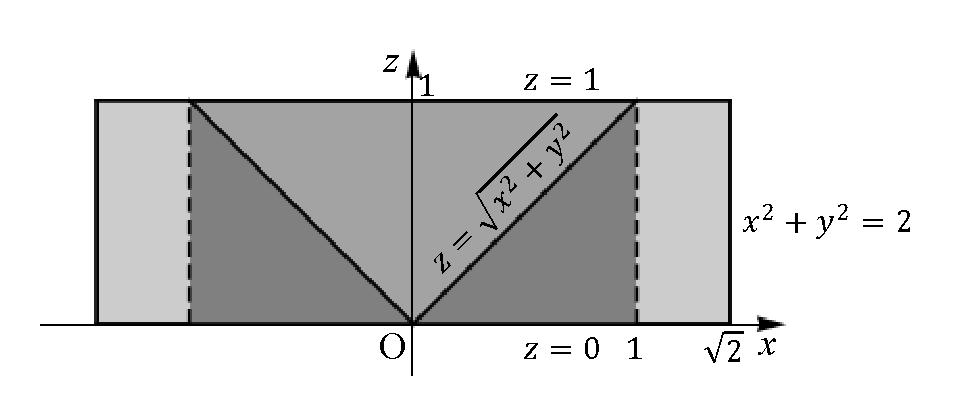
\includegraphics[height=0.2\textheight]{Figures19/Fig12-4-7-2.pdf}
%\end{center}
%\caption{习题12.4 7.题积分域在$xOz$坐标面上的截面}
%\label{12-4-7}
%\end{figure}

\item计算三重积分$\IIInt\Omega{(3x^2+5y^2+7z^2)}V,\Omega:\ x^2+y^2+z^2\leqslant R^2$.

\begin{figure}[H]
\begin{center}
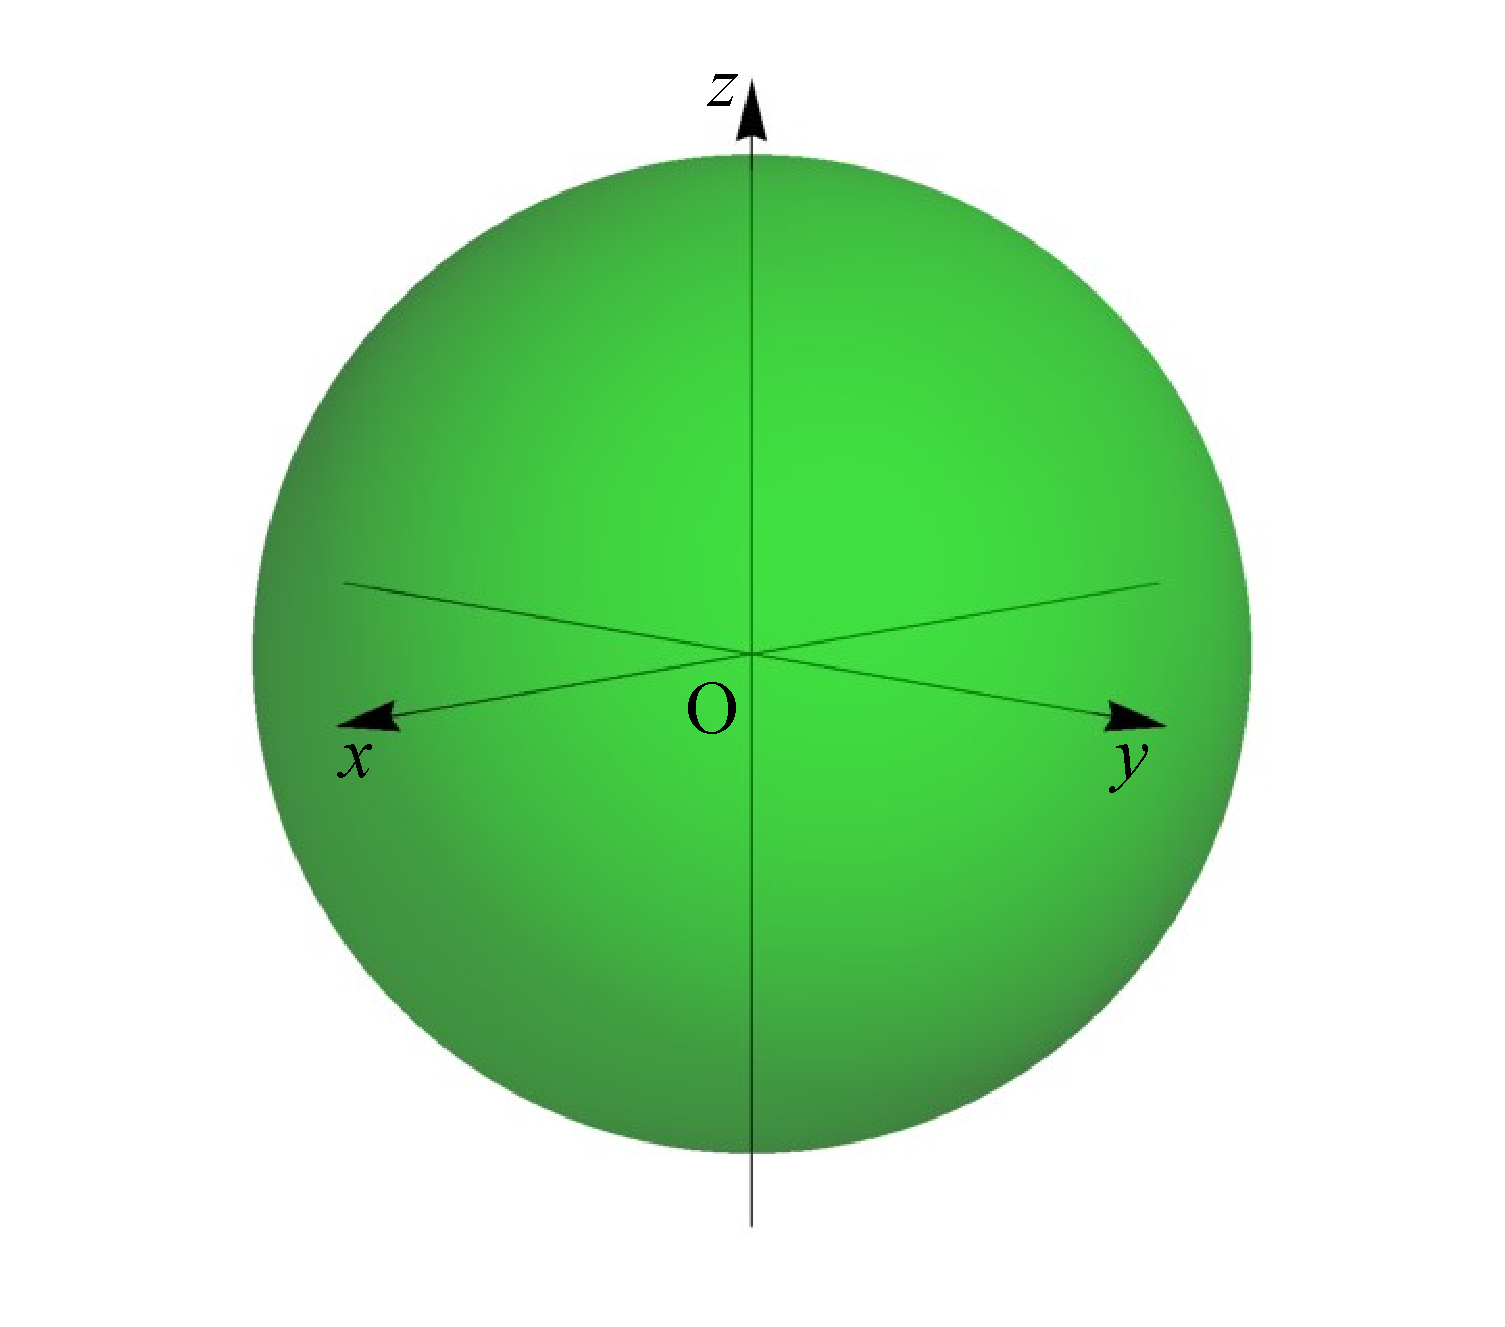
\includegraphics[height=0.4\textheight]{Figures19/Fig12-4-8.pdf}
\end{center}
\caption{习题12.4 8.题积分域}
\label{12-4-8}
\end{figure}

解:$\IIInt\Omega{z^2}V=\Int{-R}R{z^2}z\varIInt{\Omega_z}{}xy=\Int{-R}R{z^2\pi(R^2-z^2)}z=\frac4{15}\pi R^5$,

由对称性可知$\IIInt\Omega{x^2}V=\IIInt\Omega{y^2}V=\IIInt\Omega{z^2}V$,

$\therefore\IIInt\Omega{(3x^2+5y^2+7z^2)}V=(3+5+7)\IIInt\Omega{z^2}V=4\pi R^5$.

\item设$F(t)=\varIIInt\Omega{[z^2+f(x^2+y^2)]}xyz$,其中$f(u)$连续,$\Omega$为$0\leqslant z\leqslant h,x^2+y^2\leqslant t^2$. 试求$\frac{\mathrm dF}{\mathrm dt}\Big|_{t=0}$和$\LIM t0\frac1{t^2}F(t)$.

解:$F(t)=\varIIInt\Omega{[z^2+f(x^2+y^2)]}xyz=\Int0{2\pi}{}\theta\Int0t{}r\Int0h{[z^2+f(r^2)]r}z\\
=2\pi\Int0t{[\frac13rz^3+rf(r)z]\big|_0^h}r=2\pi\Int0t{[\frac13h^3r+hrf(r)]}r$,

$\therefore\frac{\mathrm dF}{\mathrm dt}=2\pi[\frac13h^3t+htf(t)]$,

$\therefore\frac{\mathrm dF}{\mathrm dt}\Big|_{t=0}=0$.

$\therefore\LIM t0\frac1{t^2}F(t)=\LIM t0\frac{\frac{\mathrm dF}{\mathrm dt}}{2t}=\LIM t0\frac{2\pi[\frac13h^3t+htf(t)]}{2t}=\LIM t0\pi[\frac13h^3+hf(t)]=\pi[\frac13h^3+hf(0)]$.

\item设$f(x)$在$[0,1]$上连续,证明:
\[
\Int01{}x\Int x1{}y\Int xy{f(x)f(y)f(z)}z=\frac16(\Int01{f(x)}x)^3.
\]
证明:设$F(u)=\Int0u{f(t)}t$,

$\because f(x)$在$[0,1]$上连续,

$\therefore F'(u)=f(u)$,

方法1:
$\therefore\Int01{}x\Int x1{}y\Int xy{f(x)f(y)f(z)}z=\Int01{f(x)}x\Int x1{f(y)}y\Int xy{f(z)}z\\
=\Int01{f(x)}x\Int x1{f(y)}y[\Int 0y{f(z)}z-\Int0x{f(z)}z]\\
=\Int01{f(x)}x\Int x1{f(y)[F(y)-F(x)]}y\\
=\Int01{f(x)}x\Int x1{[F(y)-F(x)]}{F(y)}\\
=\Int01{f(x)}x\{F(y)[F(y)-F(x)]\big|_x^1-\Int x1{F(y)}{F(y)}\}\\
=\Int01{f(x)}x\{F(1)[F(1)-F(x)]-\frac12[F(y)]^2\big|_x^1\}\\
=\Int01{f(x)}x\{F(1)[F(1)-F(x)]-\frac12[F(1)]^2+\frac12[F(x)]^2\}\\
=\Int01{f(x)}x\{\frac12[F(1)]^2-F(1)F(x)+\frac12[F(x)]^2\}\\
=\Int01{f(x)}x\frac12[F(1)-F(x)]^2=\Int01{\frac12[F(1)-F(x)]^2}{F(x)}\\
=-\frac12\Int01{[F(1)-F(x)]^2}{[F(1)-F(x)]}\\
=-\frac16[F(1)-F(x)]^3\big|_0^1\\
=\frac16[F(1)]^3\\
=\frac16(\Int01{f(x)}x)^3$.

方法2:$\therefore\Int01{}x\Int x1{}y\Int xy{f(x)f(y)f(z)}z\\
=\Int01{f(x)}x\Int x1{f(y)}y\Int xy{f(z)}z\\
=\Int01{f(x)}x\Int x1{f(y)}y[\Int 0y{f(z)}z-\Int0x{f(z)}z]\\
=\Int01{f(x)}x\Int x1{f(y)[F(y)-F(x)]}y\\
=\Int01{f(x)}x\Int x1{[F(y)-F(x)]}{[F(y)-F(x)]}\\
=\Int01{f(x)}x\frac12[F(y)-F(x)]\big|_x^1\\
=\Int01{f(x)}x\frac12[F(1)-F(x)]^2\\
=\Int01{\frac12[F(1)-F(x)]^2}{F(x)}\\
=-\frac12\Int01{[F(1)-F(x)]^2}{[F(1)-F(x)]}\\
=-\frac16[F(1)-F(x)]^3\big|_0^1\\
=\frac16[F(1)]^3\\
=\frac16(\Int01{f(x)}x)^3$.

\item求由$(x^2+y^2)^2=8x^3$围成的区域的面积.

\begin{figure}[H]
\begin{center}
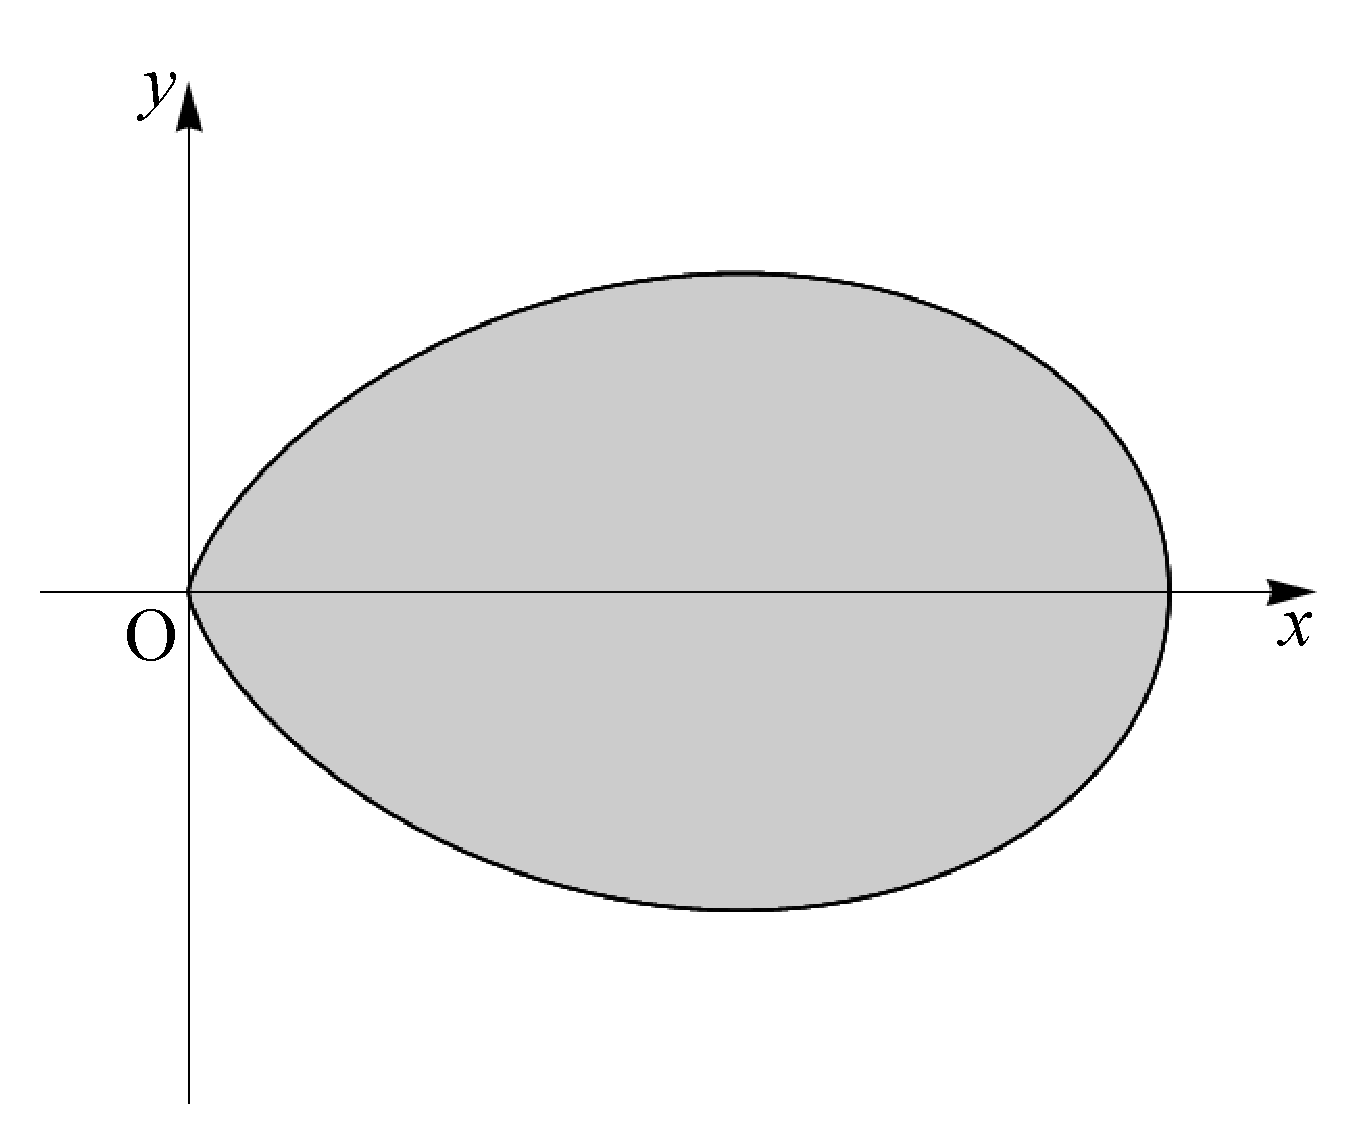
\includegraphics[height=0.4\textheight]{Figures19/Fig12-4-11.pdf}
\end{center}
\caption{习题12.4 11.题积分域}
\label{12-4-11}
\end{figure}

解:$(x^2+y^2)^2=8x^3$在极坐标系中的方程为$r=8\cos^3\theta$,且满足$\cos^3\theta\geqslant0$,即$-\frac\pi2\leqslant\theta\leqslant\frac\pi2$,

$\therefore$该区域用极坐标表示为$D=\Set{(r,\theta)}{0\leqslant r\leqslant8\cos^3\theta,-\frac\pi2\leqslant\theta\leqslant\frac\pi2}$,

$S=\IInt D{}\sigma=\Int{-\frac\pi2}{\frac\pi2}{}\theta\Int0{8\cos^3\theta}rr=\Int{-\frac\pi2}{\frac\pi2}{}\theta\frac12r^2\big|_0^{8\cos^3\theta}=32\Int{-\frac\pi2}{\frac\pi2}{\cos^6\theta}\theta=64\Int0{\frac\pi2}{\cos^6\theta}\theta\\
=64\frac{5\cdot3\cdot1}{6\cdot4\cdot2}\cdot\frac\pi2=10\pi$.

\item求由$r\leqslant a(1+\cos\theta)$与$x^2+y^2\geqslant a^2$确定的平面图形的面积.

\begin{figure}[H]
\begin{center}
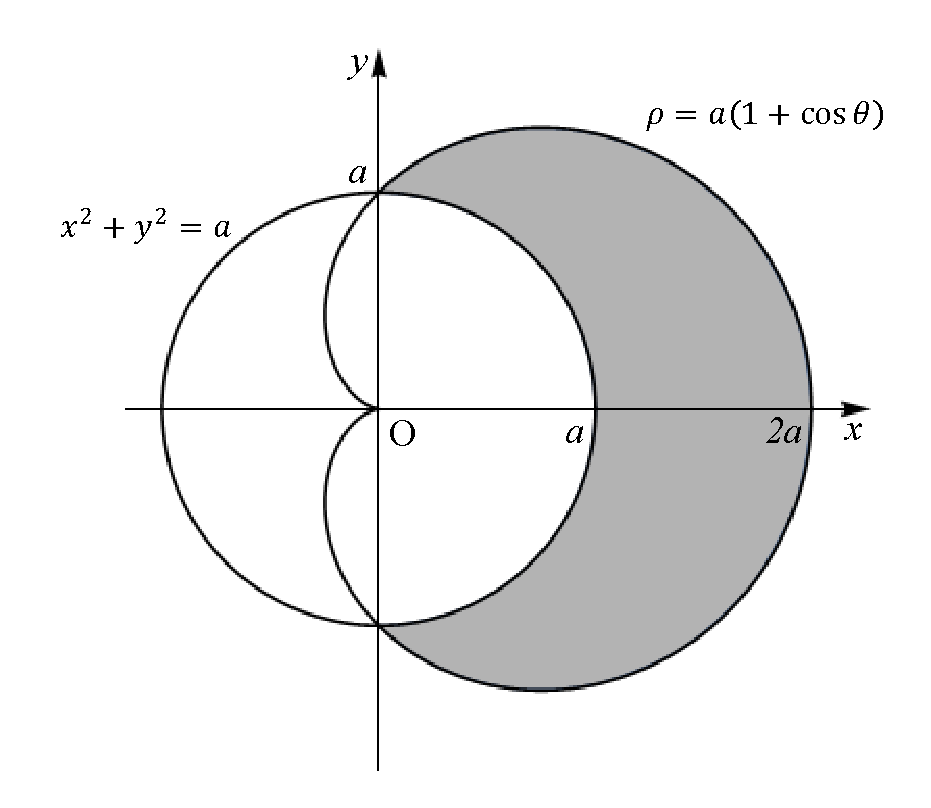
\includegraphics[height=0.4\textheight]{Figures19/Fig12-4-12.pdf}
\end{center}
\caption{习题12.4 12.题图示}
\label{12-4-12}
\end{figure}

解:圆$x^2+y^2=a^2$的极坐标表示为$r=a$,由$\begin{cases}
r=a,\\
r=a(1+\cos\theta),
\end{cases}$得$\theta=\pm\frac\pi2$,

该平面图形可表示为$D=\Set{(r,\theta)}{a\leqslant r\leqslant a(1+\cos\theta),-\frac\pi2\leqslant\theta\leqslant\frac\pi2}$,

$\therefore S=\Int D{}\sigma=\Int{-\frac\pi2}{\frac\pi2}{}\theta\Int a{a(1+\cos\theta)}rr=\Int{-\frac\pi2}{\frac\pi2}{}\theta\frac12r^2\big|_a^{a(1+\cos\theta)}=\frac12a^2\Int{-\frac\pi2}{\frac\pi2}{[(1+\cos\theta)^2-1]}\theta\\
=\frac12a^2\Int{-\frac\pi2}{\frac\pi2}{(2\cos\theta+\cos^2\theta)}\theta=a^2\Int0{\frac\pi2}{(2\cos\theta+\cos^2\theta)}\theta=a^2(2\cdot1+\frac12\cdot\frac\pi2)=(2+\frac\pi4)a^2$.

\item求由抛物面$z=x^2+y^2$与球面$z=\sqrt{6-x^2-y^2}$所围空间图形的体积.

\begin{figure}[H]
\begin{center}
\subfigure[积分域]{\label{12-4-13-1}
{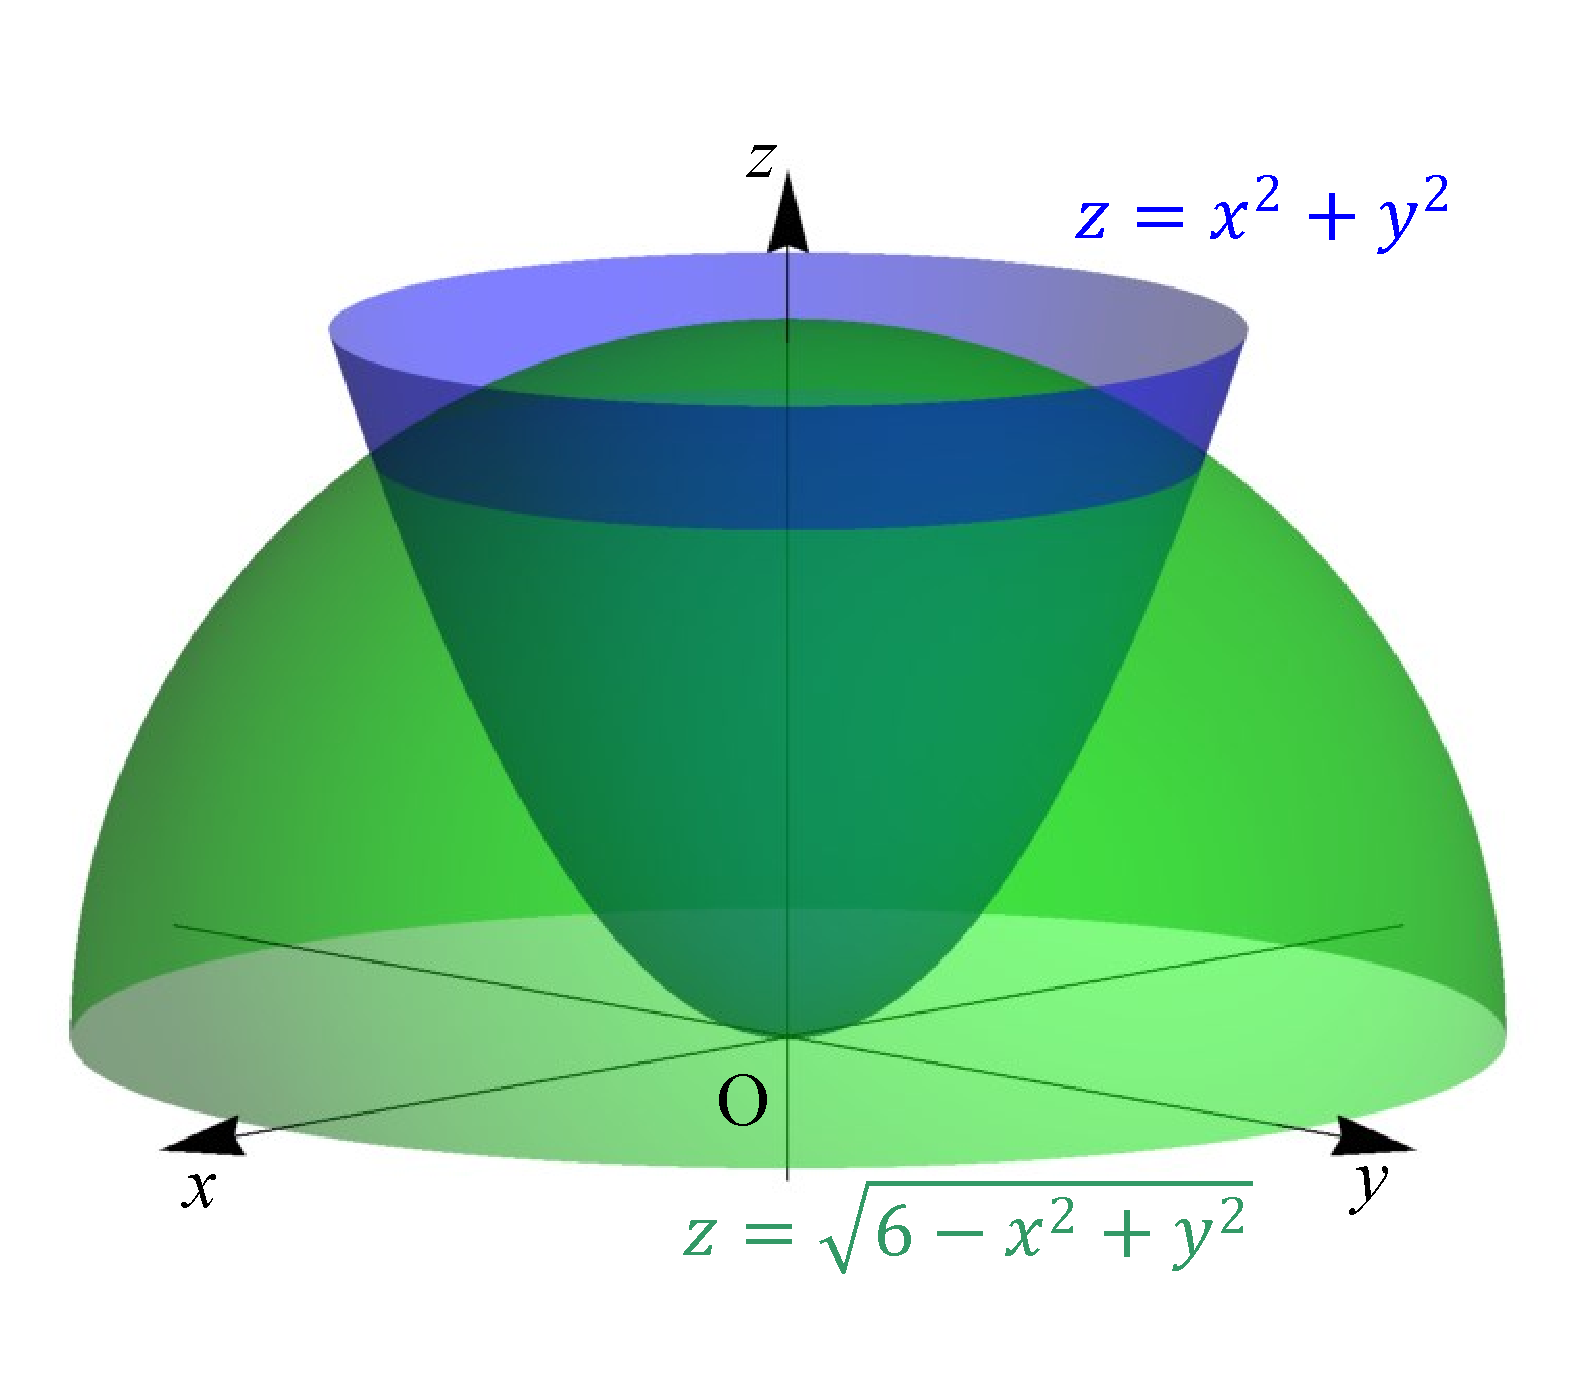
\includegraphics[height=0.4\textheight]{Figures19/Fig12-4-13-2.pdf} }}\\
\subfigure[积分域在$xOz$坐标面上的截面]{\label{12-4-13-2}
{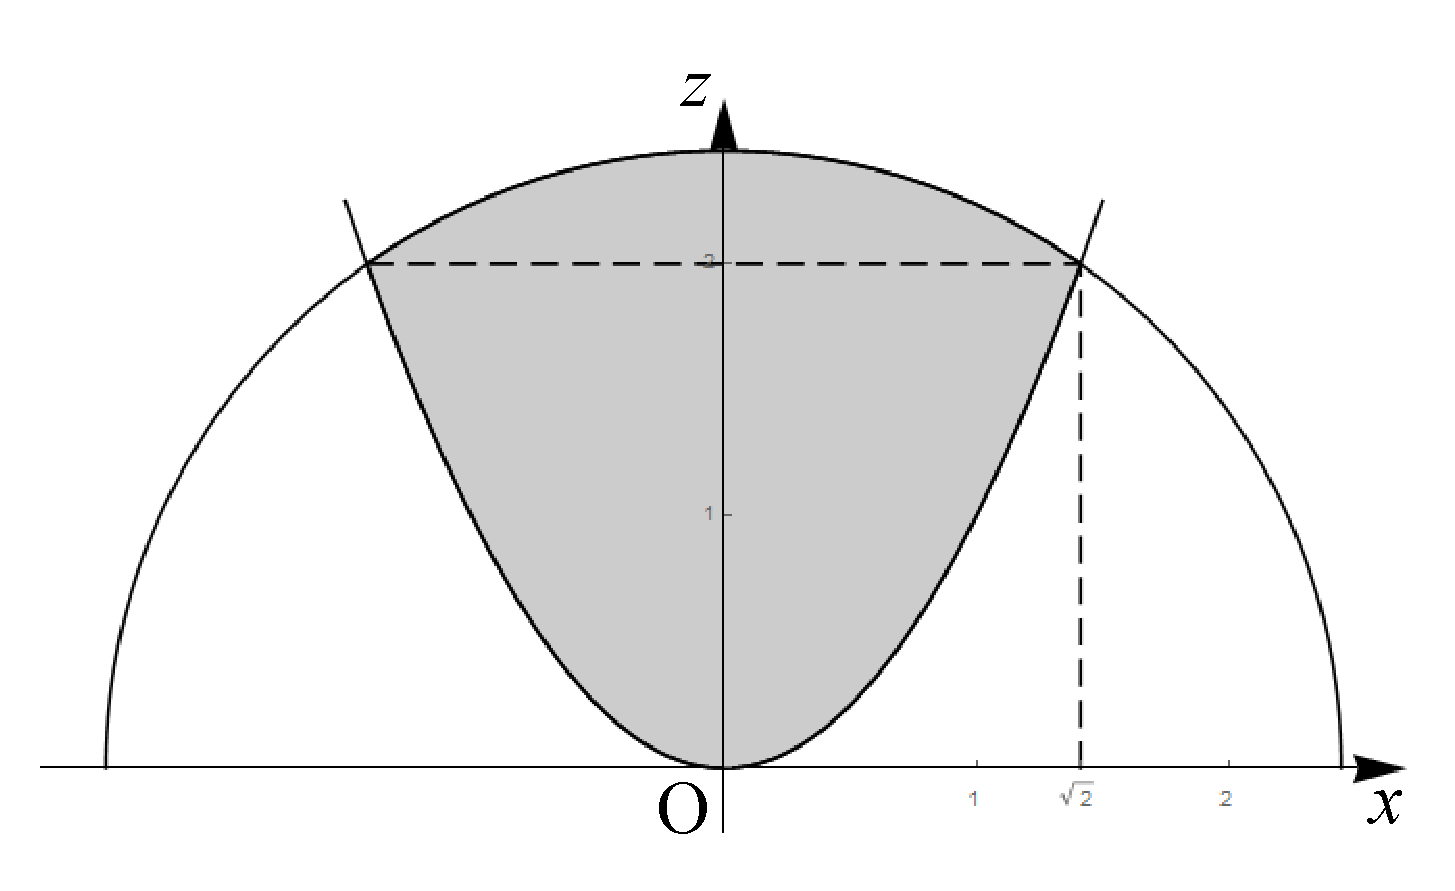
\includegraphics[height=0.3\textheight]{Figures19/Fig12-4-13-1.pdf} }}
\end{center}
\caption{习题12.4 13.题图示}
\label{12-4-13}
\end{figure}

解:由$\begin{cases}
z=x^2+y^2,\\
z=\sqrt{6-x^2-y^2},
\end{cases}$得$\begin{cases}
z=2,\\
x^2+y^2=2,
\end{cases}$该空间图形可表示为\\
$\Omega=\Set{(x,y)}{0\leqslant z\leqslant2,x^2+y^2\leqslant z}\cup\Set{(x,y)}{2\leqslant z\leqslant\sqrt6,x^2+y^2\leqslant6-z^2}$,

$\therefore\IIInt\Omega{}V=\Int02{}z\varIInt{\Omega_z}{}xy+\Int2{\sqrt6}{}z\varIInt{\Omega_z}{}xy=\Int02{\pi z}z+\Int2{\sqrt6}{\pi(6-z^2)}z\\
=\pi\frac12z^2\big|_0^2+\pi(6z-\frac13z^3)\big|_2^{\sqrt6}=2\pi+\pi(6\sqrt6-\frac13\cdot6\sqrt6-12+\frac83)=\pi(4\sqrt6-\frac{22}3)$.
%
%注:如图~\ref{12-4-13}所示.
%\begin{figure}[H]
%\begin{center}
%\includegraphics[height=0.4\textheight]{Figures19/Fig12-4-13.pdf}
%\end{center}
%\caption{习题12.4 13.题积分域在$xOz$平面上的截面图形}
%\label{12-4-13}
%\end{figure}

\item利用三重积分计算曲面所围成的空间区域的体积:\\
(1)$1\leqslant x^2+y^2\leqslant2x,0\leqslant z\leqslant xy$;\\
(2)$x^2+y^2+z^2=a^2,x^2+y^2+z^2=b^2,x^2+y^2=z^2,z\geqslant0,0<a<b$.

解:(1)
\begin{figure}[H]
\begin{center}
\subfigure[积分域]{\label{12-4-14-1-1}
{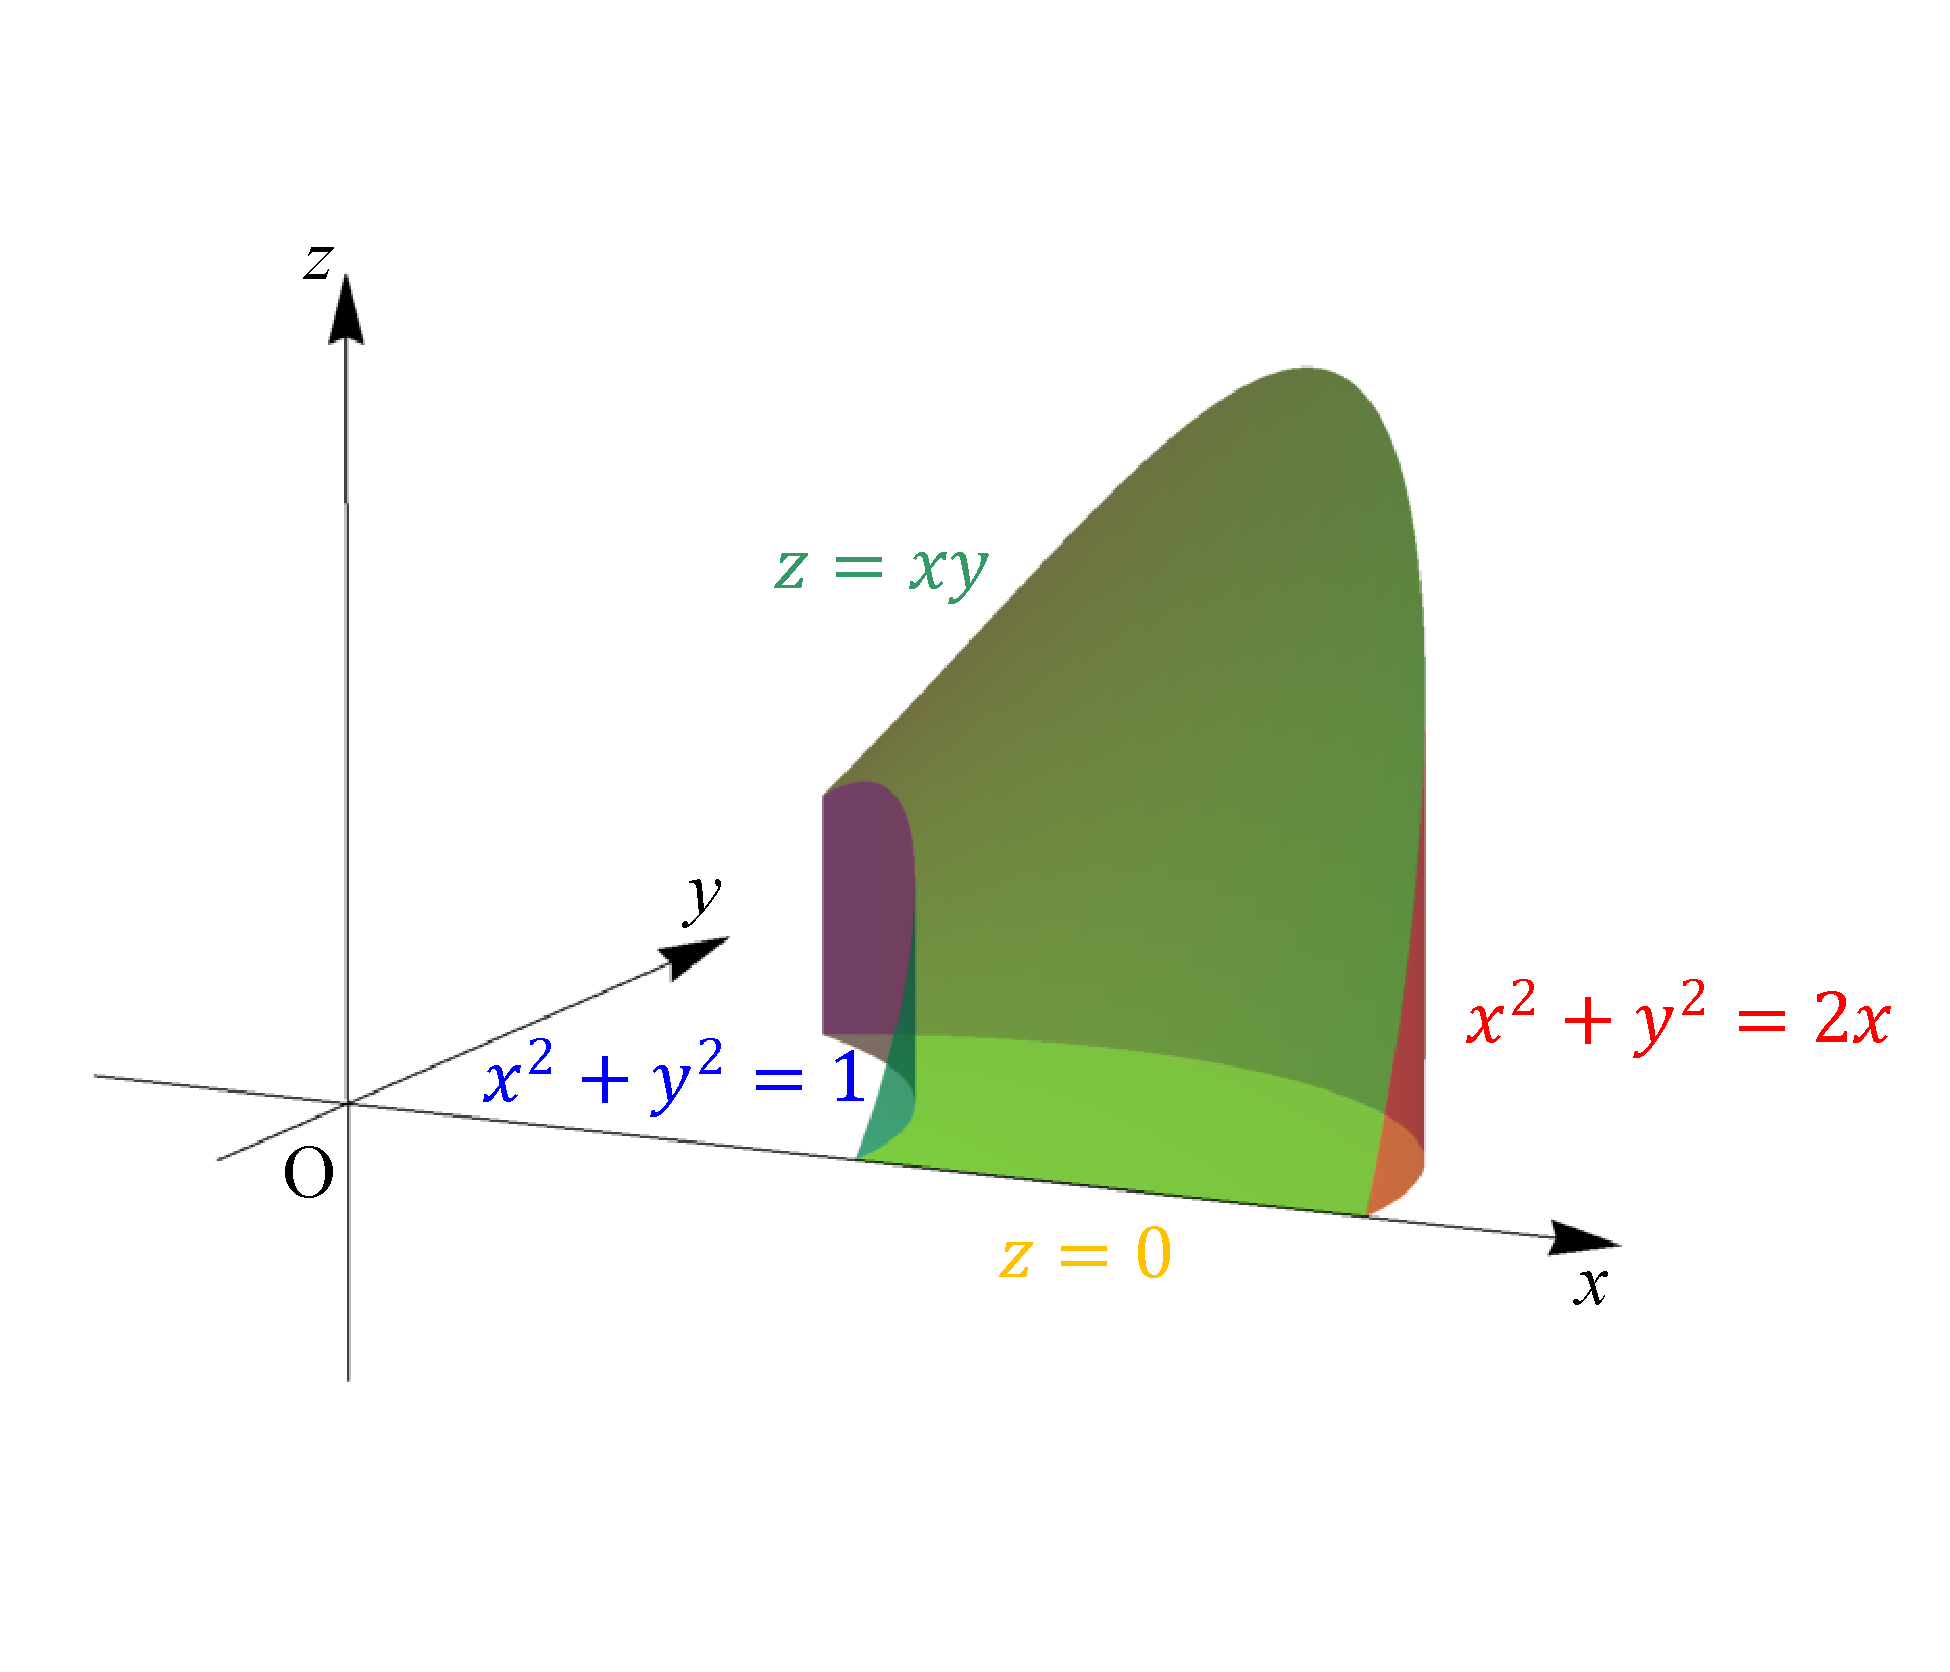
\includegraphics[height=0.5\textheight]{Figures19/Fig12-4-14-1-1.pdf} }}\\
\subfigure[积分域在$xOy$平面上的投影]{\label{12-4-14-1-1}
{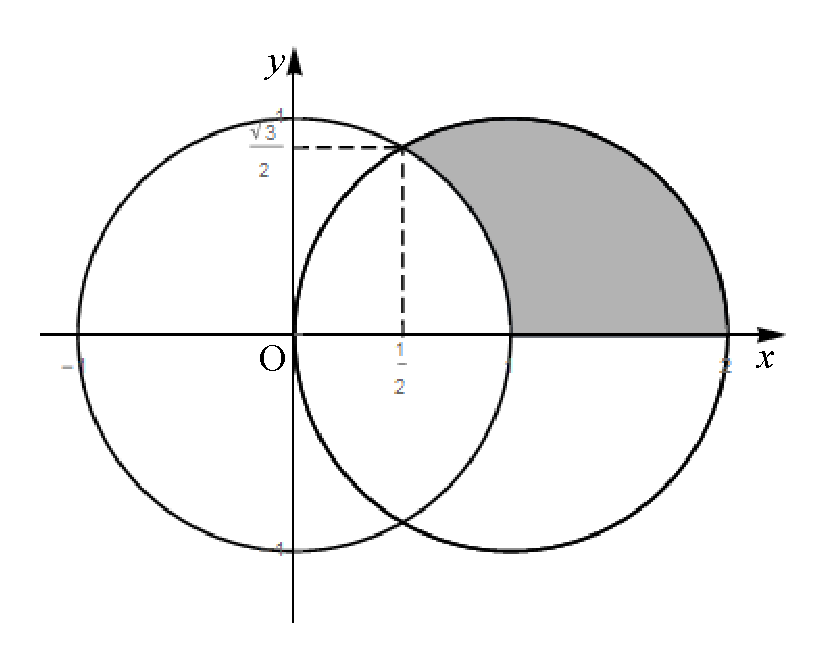
\includegraphics[height=0.4\textheight]{Figures19/Fig12-4-14-1-2.pdf} }}
\end{center}
\caption{习题12.4 14.(1)题图示}
\label{12-4-14-1}
\end{figure}

$\because0\leqslant z\leqslant xy$,

$\therefore xy\geqslant0$,

$\therefore$区域$\Omega=\Set{(x,y)}{1\leqslant x^2+y^2\leqslant2x,0\leqslant z\leqslant xy}$在柱坐标系下可表示为\\
$\Omega=\Set{(r,\theta,z)}{0\leqslant z\leqslant r^2\sin\theta\cos\theta,1\leqslant r\leqslant2\cos\theta,0\leqslant\theta\leqslant\frac\pi3}$,

$\therefore\IIInt\Omega{}V=\Int0{\frac\pi3}{}\theta\Int1{2\cos\theta}{}r\Int0{r^2\sin\theta\cos\theta}{r}z=\Int0{\frac\pi3}{}\theta\Int1{2\cos\theta}{r^3\sin\theta\cos\theta}r\\
=\Int0{\frac\pi3}{\sin\theta\cos\theta\frac14r^4\big|_1^{2\cos\theta}}\theta=\Int0{\frac\pi3}{\sin\theta\cos\theta\frac14\cdot(16\cos^4\theta-1)}\theta\\
=4\Int0{\frac\pi3}{\cos^5\theta\sin\theta}\theta-\frac14\Int0{\frac\pi3}{\sin\theta\cos\theta}\theta=-4\cdot\frac16\cos^6\theta\big|_0^{\frac\pi3}-\frac14\cdot\frac12\sin^2\theta\big|_0^{\frac\pi3}\\
=\frac23(1-\frac1{64})-\frac18\cdot\frac34=\frac9{16}$.
%
%注:如图~\ref{12-4-14-1}所示.
%\begin{figure}[H]
%\begin{center}
%\includegraphics[height=0.4\textheight]{Figures19/Fig12-4-14-1.pdf}
%\end{center}
%\caption{习题12.4 14.(1)题积分域在$xOy$平面上的投影}
%\label{12-4-14-1}
%\end{figure}

(2)
\begin{figure}[H]
\begin{center}
\includegraphics[height=0.4\textheight]{Figures19/Fig12-4-14-2.pdf}
\end{center}
\caption{习题12.4 14.(2)题积分域}
\label{12-4-14-2}
\end{figure}

已知区域$\Omega$在球坐标系下可表示为$\Omega=\Set{(r,\theta,\varphi)}{a\leqslant r\leqslant b,0\leqslant\theta\leqslant2\pi,0\leqslant\varphi\leqslant\frac\pi4}$,

$\therefore\IIInt\Omega{}V=\Int0{2\pi}{}\theta\Int0{\frac\pi4}{}\varphi\Int ab{r^2\sin\varphi}r=\Int0{2\pi}{}\theta\Int0{\frac\pi4}{\frac13r^3\big|_a^b\sin\varphi}\varphi=\frac23\pi(b^3-a^3)\Int0{\frac\pi4}{\sin\varphi}\varphi\\
=\frac23\pi(b^3-a^3)(-\cos\varphi)\big|_0^{\frac\pi4}=\frac23(1-\frac{\sqrt2}2)\pi(b^3-a^3)$.

\item求由平面$a_1x+b_1y+c_1z=\pm h_1,a_2x+b_2y+c_2z=\pm h_2,a_3x+b_3y+c_3z=\pm h_3$所围成平行六面体的体积.

解:令$\begin{cases}
u=a_1x+b_1y+c_1z,\\
v=a_2x+b_2y+c_2z,\\
w=a_3x+b_3y+c_3z,
\end{cases}$不妨设$h_1>0,h_2>0,h_3>0$,则该平行六面体可表示为$\Omega=\Set{(u,v,w)}{-h_1\leqslant u\leqslant h_1,-h_2\leqslant v\leqslant h_2,-h_3\leqslant w\leqslant h_3}$,

$\frac{\mathrm D(u,v,w)}{\mathrm D(x,y,z)}=\begin{vmatrix}
a_1&b_1&c_1\\
a_2&b_2&c_2\\
a_3&b_3&c_3
\end{vmatrix}=\det A$,

当$\det A\neq0$时,\\
$\varIIInt\Omega{}xyz=\varIIInt\Omega{|\frac{\mathrm D(x,y,z)}{\mathrm D(u,v,w)}|}uvw=\varIIInt\Omega{\frac1{|\frac{\mathrm D(u,v,w)}{\mathrm D(x,y,z)}|}}uvw=\varIIInt\Omega{\frac1{|\det A|}}uvw\\
=\frac1{|\det A|}\varIIInt\Omega{}uvw=\frac{2h_1\cdot2h_2\cdot2h_3}{|\det A|}=\frac{8h_1h_2h_3}{|\det A|}$.

\item设$D=\Set{(x,y)}{4\leqslant x^2+y^2\leqslant9}$是一平面圆环,每点的质量密度为$\mu(x,y)=1+x^2+y^2$,试求:\\
(1)$D$在第一象限部分的重心;\\
(2)$D$关于$y$轴的转动惯量.

\begin{figure}[H]
\begin{center}
\includegraphics[height=0.4\textheight]{Figures19/Fig12-4-16.pdf}
\end{center}
\caption{习题12.4 16.题图示}
\label{12-4-16}
\end{figure}

解:(1)$D$在第一象限部分用极坐标表示为$D_1=\Set{(r,\theta)}{2\leqslant r\leqslant3,0\leqslant\theta\leqslant\frac\pi2}$,

$\therefore\bar{x}=\frac{\varIInt{D_1}{x\mu(x,y)}xy}{\varIInt{D_1}{\mu(x,y)}xy}=\frac{\Int0{2\pi}{}\theta\Int23{r\cos\theta(1+r^2)r}r}{\Int0{2\pi}{}\theta\Int23{(1+r^2)r}r}=\frac{\Int0{\frac\pi2}{\cos\theta}\theta\Int23{(r^2+r^4)}r}{\frac\pi2(\frac12r^2+\frac14r^4)\big|_2^3}=\frac{1\cdot(\frac13r^3+\frac15r^5)\big|_2^3}{\frac\pi2(\frac92+\frac{81}4-2-4)}=\frac{9+\frac{243}5-\frac83-\frac{32}5}{\frac\pi2(\frac{99}4-6)}\\
=\frac{5824}{1125\pi}$,

由对称性可知$\bar{y}=\bar{x}$,故$D$在第一象限部分的重心为$(\frac{5824}{1125\pi},\frac{5824}{1125\pi})$.

(2)$D$关于$y$轴的转动惯量\\
$J_y=\varIInt D{x^2\mu(x,y)}xy=\Int0{2\pi}{}\theta\Int23{r^2\cos^2\theta(1+r^2)r}r=\Int0{2\pi}{\cos^2\theta}\theta\Int23{(r^3+r^5)}r\\
=4\Int0{\frac\pi2}{\cos^2\theta}\theta(\frac14r^4+\frac16r^6)\big|_2^3=4\cdot\frac\pi4(\frac14\cdot81+\frac16\cdot729-4-\frac16\cdot64)=\frac{1525}{12}\pi$.

\item设球$x^2+y^2+z^2\leqslant2az$中各点的密度为$\rho=\frac1{\sqrt{x^2+y^2+z^2}}$,求球的质量与质心.

\begin{figure}[H]
\begin{center}
\includegraphics[height=0.4\textheight]{Figures19/Fig12-4-17.pdf}
\end{center}
\caption{习题12.4 17.题图示}
\label{12-4-17}
\end{figure}

解:该球用球坐标表示为$\Omega=\Set{(r,\theta,\varphi)}{0\leqslant r\leqslant2a\cos\varphi,0\leqslant\varphi\leqslant\frac\pi2,0\leqslant\theta\leqslant2\pi}$,

质量$m=\IIInt\Omega\rho V=\Int0{2\pi}{}\theta\Int0{\frac\pi2}{}\varphi\Int0{2a\cos\varphi}{\frac1rr^2\sin\varphi}r=2\pi\Int0{\frac\pi2}{}\varphi(\frac12r^2\sin\varphi)\big|_0^{2a\cos\varphi}\\
=2\pi\Int0{\frac\pi2}{(\frac124a^2\cos^2\varphi\sin\varphi)}\varphi=-4\pi a^2\frac13\cos^3\varphi\big|_0^{\frac\pi2}=\frac43\pi a^2$,

由对称性可知$\bar{x}=\bar{y}=0$,

$M_{xy}=\IIInt\Omega{z\rho}V=\Int0{2\pi}{}\theta\Int0{\frac\pi2}{}\varphi\Int0{2a\cos\varphi}{r\cos\varphi\frac1rr^2\sin\varphi}r=2\pi\Int0{\frac\pi2}{}\varphi\cos\varphi\sin\varphi\frac13r^3\big|_0^{2a\cos\varphi}\\
=2\pi\Int0{\frac\pi2}{\frac83a^3\cos^4\varphi\sin\varphi}\varphi=-\frac{16}3\pi a^3\frac15\cos^5\varphi\big|_0^{\frac\pi2}=\frac{16}{15}\pi a^3$,

$\therefore\bar{z}=\frac{M_{xy}}m=\frac{\frac{16}{15}\pi a^3}{\frac43\pi a^2}=\frac45a$,

故质心为$(0,0,\frac45a)$.

\item设$\Omega$由$z=x^2+y^2$及$z=2x$围成,密度$\rho=y^2$,求它对$z$轴的转动惯量.

\begin{figure}[H]
\begin{center}
\includegraphics[height=0.4\textheight]{Figures19/Fig12-4-18.pdf}
\end{center}
\caption{习题12.4 18.题图示}
\label{12-4-18}
\end{figure}

解:由$\begin{cases}
z=x^2+y^2,\\
z=2x,
\end{cases}$得两曲面的投影柱面$x^2+y^2=2x$,

$\therefore$积分域在柱坐标系下表示为$\Omega=\Set{(r,\theta,z)}{r^2\leqslant z\leqslant 2r\cos\theta,0\leqslant r\leqslant2\cos\theta,-\frac\pi2\leqslant\theta\leqslant\frac\pi2}$,

$\therefore J_z=\varIIInt\Omega{(x^2+y^2)\rho}xyz=\Int{-\frac\pi2}{\frac\pi2}{}\theta\Int0{2\cos\theta}{}r\Int{r^2}{2r\cos\theta}{r^2r^2\sin^2\theta\cdot r}z\\
=\Int{-\frac\pi2}{\frac\pi2}{}\theta\Int0{2\cos\theta}{r^5\sin^2\theta(2r\cos\theta-r^2)}r=\Int{-\frac\pi2}{\frac\pi2}{}\theta\Int0{2\cos\theta}{(2r^6\sin^2\theta\cos\theta-r^7\sin^2\theta)}r\\
=\Int{-\frac\pi2}{\frac\pi2}{(\frac27r^7\sin^2\theta\cos\theta-\frac18r^8\sin^2\theta)\big|_0^{2\cos\theta}}\theta=\Int{-\frac\pi2}{\frac\pi2}{(\frac{2^8}7\cos^8\theta\sin^2\theta-\frac{2^8}8\cos^8\theta\sin^2\theta)}\theta\\
=\frac{2^8}{56}\cdot2\Int0{\frac\pi2}{\cos^8\theta\sin^2\theta}\theta=\frac{64}7\Int0{\frac\pi2}{\cos^8\theta(1-\cos^2\theta)}\theta=\frac{64}7(\Int0{\frac\pi2}{\cos^8\theta}\theta-\Int0{\frac\pi2}{\cos^{10}\theta}\theta)\\
=\frac{64}7(\frac{7\cdot5\cdot3\cdot1}{8\cdot6\cdot4\cdot2}\cdot\frac\pi2-\frac{9\cdot7\cdot5\cdot3\cdot1}{10\cdot8\cdot6\cdot4\cdot2}\cdot\frac\pi2)=\frac{64}7(\frac1{10}\cdot\frac{7\cdot5\cdot3\cdot1}{8\cdot6\cdot4\cdot2})\cdot\frac\pi2=\frac\pi8$.

\item试证曲面$z=x^2+y^2+a(a>0)$上任意点处的切平面与曲面$z=x^2+y^2$所围成的空间区域的体积是一常数.

\begin{figure}[H]
\begin{center}
\subfigure[积分域]{\label{12-4-19-1}
{\includegraphics[height=0.5\textheight]{Figures19/Fig12-4-19-1.pdf} }}\\
\subfigure[积分域在$lOz$平面上的截面图形,$lOz$平面由$Oz$轴与切点确定.]{\label{12-4-19-2}
{\includegraphics[height=0.4\textheight]{Figures19/Fig12-4-19-2.pdf} }}
\end{center}
\caption{习题12.4 19.题图示}
\label{12-4-19}
\end{figure}

证明:设$(x_0,y_0,z_0)$是曲面$z=x^2+y^2+a$上的任意点,则$z_0=x_0^2+y_0^2+a$,曲面在该点的法向量为$\bm n=(2x,2y,-1)\big|_{(x_0,y_0,z_0)}=(2x_0,2y_0,-1)$,

$\therefore$切平面的方程为$2x_0(x-x_0)+2y_0(y-y_0)-(z-z_0)=0$,\\
即$2x_0x+2y_0y-z=2x_0^2+2y_0^2-z_0=2(z_0-a)-z_0=z_0-2a$,

由$\begin{cases}
z=x^2+y^2,\\
2x_0x+2y_0y-z=z_0-2a,
\end{cases}$得切平面与曲面$z=x^2+y^2$的交线所在的投影柱面为$x^2+y^2-2x_0x-2y_0y+z_0-2a=0$,\\
即$(x-x_0)^2+(y-y_0)^2=x_0^2+y_0^2-z_0+2a=z_0-a-z_0+2a=a$,

令$\begin{cases}
x=x_0+r\cos\theta,\\
y=y_0+r\sin\theta,\\
z=z,
\end{cases}\frac{\mathrm D(x,y)}{\mathrm D(r,\theta)}=\begin{vmatrix}
\cos\theta&-r\sin\theta&0\\
\sin\theta&r\cos\theta&0\\
0&0&1
\end{vmatrix}=r$\\
切平面用$r,\theta,z$坐标表示为$2x_0(x_0+r\cos\theta)+2y_0(y_0+r\sin\theta)-z\\
=2x_0r\cos\theta+2y_0r\sin\theta-z+2x_0^2+2y_0^2=z_0-2a$,\\
即$z=2x_0r\cos\theta+2y_0r\sin\theta+2x_0^2+2y_0^2-z_0+2a\\
=2x_0r\cos\theta+2y_0r\sin\theta+2(z_0-a)-z_0+2a=2x_0r\cos\theta+2y_0r\sin\theta+z_0$,

曲面$z=x^2+y^2$用$r,\theta,z$坐标表示为$z=(x_0+r\cos\theta)^2+(y_0+r\sin\theta)^2\\
=r^2+2x_0r\cos\theta+2y_0r\sin\theta+x_0^2+y_0^2=r^2+2x_0r\cos\theta+2y_0r\sin\theta+z_0-a$,

$\therefore$所求空间区域$\Omega=\{(r,\theta,z)\ \vert\ 0\leqslant\theta\leqslant2\pi,0\leqslant r\leqslant\sqrt a,\\
2x_0r\cos\theta+2y_0r\sin\theta+z_0\leqslant z\leqslant r^2+2x_0r\cos\theta+2y_0r\sin\theta+z_0-a \}$,

$\therefore\varIIInt\Omega{}xyz=\varIIInt\Omega{|\frac{\mathrm D(x,y)}{\mathrm D(r,\theta)}|}r\theta z=\Int0{2\pi}{}\theta\Int0{\sqrt a}{}r\Int{r^2+2x_0r\cos\theta+2y_0r\sin\theta+z_0-a}{2x_0r\cos\theta+2y_0r\sin\theta+z_0}{r}z\\
=\Int0{2\pi}{}\theta\Int0{\sqrt a}{r[2x_0r\cos\theta+2y_0r\sin\theta+z_0-(r^2+2x_0r\cos\theta+2y_0r\sin\theta+z_0-a)]}r\\
=\Int0{2\pi}{}\theta\Int0{\sqrt a}{r(a-r^2)}r=2\pi(\frac12ar^2-\frac14r^4)\big|_0^{\sqrt a}=\frac\pi2 a^2$,

故曲面$z=x^2+y^2+a(a>0)$上任意点处的切平面与曲面$z=x^2+y^2$所围成的空间区域的体积是一常数.

%注:如图~\ref{12-4-19}所示.
%\begin{figure}[H]
%\begin{center}
%\includegraphics[height=0.3\textheight]{Figures19/Fig12-4-19-2.pdf}
%\end{center}
%\caption{习题12.4 19.题积分域在$lOz$平面上的截面图形,$lOz$平面由$Oz$轴与切点确定.}
%\label{12-4-19}
%\end{figure}
\end{enumerate}
\end{document} 
\documentclass[12pt,UTF8]{ctexart}
\usepackage{ctex,amsmath,amssymb,geometry,fancyhdr,bm,amsfonts,mathtools,extarrows,graphicx,url,enumerate,color,float,multicol,wasysym}
\usepackage{subfigure}
 
\allowdisplaybreaks[4]
% 加入中文支持
\newcommand\Set[2]{\left\{#1\ \middle\vert\ #2 \right\}}
\newcommand\Lim[0]{\lim\limits_{n\rightarrow\infty}}
\newcommand\LIM[2]{\lim\limits_{#1\rightarrow#2}}
\newcommand\Ser[1]{\sum_{n=#1}^\infty}
\newcommand{\SER}[2]{\sum_{#1=#2}^\infty}
\newcommand{\Int}[4]{\varint\nolimits_{#1}^{#2}#3\mathrm d#4}
\newcommand{\aIInt}[1]{\iint\limits_{#1}}
\newcommand{\IInt}[3]{\iint\limits_{#1}#2\mathrm d#3}
\newcommand{\varIInt}[4]{\iint\limits_{#1}#2\mathrm d#3\mathrm d#4}
\newcommand{\IIInt}[3]{\iiint\limits_{#1}#2\mathrm d#3}
\newcommand{\varIIInt}[5]{\iiint\limits_{#1}#2\mathrm d#3\mathrm d#4\mathrm d#5}
\newcommand{\LInt}[3]{\varint\nolimits_{#1}#2\mathrm d#3}
\newcommand{\SIInt}[3]{\iint\limits_{#1}#2\mathrm d#3}
\geometry{a4paper,scale=0.80}
\pagestyle{fancy}
\rhead{习题12.5\&12.6}
\lhead{基础习题课讲义}
\chead{微积分B(2)}
\begin{document}
\setcounter{section}{19}
\section{第一型曲线和曲面积分}
\subsection{知识结构}
\noindent第12章重积分
	\begin{enumerate}
		\item[12.5]第一型曲线积分
		\item[12.6]曲面面积和曲面积分
			\begin{enumerate}
				\item[12.6.1]曲面面积的求法
					\begin{itemize}
						\item斜面的面积
						\item曲面$z=f(x,y)$的面积的计算公式
						\item参数方程下曲面面积的计算公式
					\end{itemize}
				\item[12.6.2]曲面积分
			\end{enumerate}
	\end{enumerate}
\subsection{习题12.5解答}
\begin{enumerate}
\item求$\LInt{L}{(x+y)}{l}$,其中$L$为以$O(0,0),A(1,0),B(0,1)$为顶点的三角形的边界.

解:$\LInt{L}{(x+y)}{l}=\LInt{OA}{(x+0)}{l}+\LInt{AB}{(x+1-x)}{l}+\LInt{OB}{(0+y)}{l}\\
=\Int01{(x+0)\sqrt{1^2+0^2}}{x}+\Int01{(x+1-x)\sqrt{1^2+(-1)^2}}{x}+\Int01{(0+y)\sqrt{0^2+1^2}}{y}\\
=\frac12+\sqrt2+\frac12=1+\sqrt2$.

{\bf注:}如图~\ref{12-5-1}所示.
\begin{figure}[H]
\begin{center}
\includegraphics[height=0.3\textheight]{Figures20/Fig12-5-1.pdf}
\end{center}
\caption{习题12.5 1.题图示}
\label{12-5-1}
\end{figure}

\item计算$\LInt L{|y|}l$,其中$L$为圆心在坐标原点的右半单位圆周.

解:设$L_1$为圆心在原点的单位圆周在第一象限的部分,极坐标下的方程为$r(\theta)=1,0\leqslant\theta\leqslant\frac\pi2$,

根据对称性可知$\LInt L{|y|}l=2\LInt{L_1}yl=2\Int0{\frac\pi2}{\sin\theta\sqrt{[r(\theta)]^2+[r'(\theta)]^2}}\theta=2\Int0{\frac\pi2}{\sin\theta}\theta=2$.

\item求$\LInt L{y^2}l$,其中$L$为摆线$x=a(t-\sin t),y=a(1-\cos t)(0\leqslant t\leqslant2\pi,a>0)$的一拱.

解:$\LInt L{y^2}l=\Int0{2\pi}{a^2(1-\cos t)^2\sqrt{[x'(t)]^2+[y'(t)]^2}}t\\
=\Int0{2\pi}{a^2(1-\cos t)^2\sqrt{[a(1-\cos t)]^2+[a\sin t]^2}}t=\Int0{2\pi}{a^2(1-\cos t)^2\sqrt{a^2(2-2\cos t)}}t\\
=a^3\Int0{2\pi}{(2\sin^2\frac t2)^2\sqrt{2\cdot2\sin^2\frac t2}}t=8a^3\Int0{2\pi}{\sin^5\frac t2}t=16a^3\Int0\pi{\sin^5u}u=32a^3\Int0{\frac\pi2}{\sin^5u}u\\
=32a^3\frac{4\cdot2}{5\cdot3}=\frac{256}{15}a^3$.

{\bf注:}如图~\ref{12-5-3}所示.
\begin{figure}[H]
\begin{center}
\includegraphics[height=0.2\textheight]{Figures20/Fig12-5-3.pdf}
\end{center}
\caption{习题12.5 3.题图示}
\label{12-5-3}
\end{figure}

\item计算$\LInt L{\sqrt{x^2+y^2}}l$,其中$L$为圆周$x^2+y^2=ax$.

解:$L$在极坐标下的方程为$r(\theta)=a\cos\theta,\frac\pi2\leqslant\theta\leqslant\frac\pi2$,

$\LInt L{\sqrt{x^2+y^2}}l=\Int{-\frac\pi2}{\frac\pi2}{r(\theta)\sqrt{[r(\theta)]^2+[r'(\theta)]^2}}\theta=\Int{-\frac\pi2}{\frac\pi2}{a\cos\theta\sqrt{[a\cos\theta]^2+[-a\sin\theta]^2}}\theta\\
=2a^2\Int0{\frac\pi2}{\cos\theta}\theta=2a^2$.

\item设$L$为椭圆$\frac{x^2}4+\frac{y^2}3=1$,周长为$a$,求$\varoint_L(2xy+3x^2+4y^2)\mathrm dl$.

解:根据对称性可知$\varoint_L2xy\mathrm dl=0$,

$\therefore\varoint_L(2xy+3x^2+4y^2)\mathrm dl=\varoint_L(3x^2+4y^2)\mathrm dl=12\varoint_L(\frac{x^2}4+\frac{y^2}3)\mathrm dl=12\varoint_L\mathrm dl=12a$.

\item设曲线为$\begin{cases}
x=\mathrm e^{-t}\cos t,\\
y=\mathrm e^{-t}\sin t,\\
z=\mathrm e^{-t},
\end{cases}0<t<+\infty$,求曲线的弧长.

解:记该曲线为$L$,其弧长为

$\LInt L{}l=\Int0{+\infty}{\sqrt{[x'(t)]^2+[y'(t)]^2+[z'(t)]^2}}t\\
=\Int0{+\infty}{\sqrt{[-\mathrm e^{-t}(\cos t+\sin t)]^2+[-\mathrm e^{-t}(\sin t-\cos t)]^2+[-\mathrm e^{-t}]^2}}t\\
=\Int0{+\infty}{\mathrm e^{-t}\sqrt{(\cos t+\sin t)^2+(\sin t-\cos t)^2+1}}t=\Int0{+\infty}{\mathrm e^{-t}\sqrt3}t=-\sqrt3\mathrm e^{-t}\big|_0^{+\infty}=\sqrt3$.

{\bf注:}如图~\ref{12-5-6}所示.
\begin{figure}[H]
\begin{center}
\includegraphics[height=0.7\textheight]{Figures20/Fig12-5-6.pdf}
\end{center}
\caption{习题12.5 6.题图示}
\label{12-5-6}
\end{figure}

\item计算$\LInt L{(x^2+y^2+z^2)}l$,其中$L$为螺旋线$x=a\cos t,y=a\sin t,z=bt(0\leqslant t\leqslant2\pi)$的一段.

解:$\LInt L{(x^2+y^2+z^2)}l=\Int0{2\pi}{(a^2\cos^2t+a^2\sin^2t+b^2t^2)\sqrt{[-a\sin t]^2+[a\cos t]^2+b^2}}t\\
=\sqrt{a^2+b^2}\Int0{2\pi}{(a^2+b^2t^2)}t=\sqrt{a^2+b^2}(a^2t+\frac13b^2t^3)\big|_0^{2\pi}=(2\pi a^2+\frac83\pi^3b^2)\sqrt{a^2+b^2}$.

{\bf注:}如图~\ref{12-5-7}所示.
\begin{figure}[H]
\begin{center}
\includegraphics[height=0.7\textheight]{Figures20/Fig12-5-7.pdf}
\end{center}
\caption{习题12.5 7.题图示}
\label{12-5-7}
\end{figure}
\end{enumerate}
\subsection{习题12.6解答}
\begin{enumerate}
\item求锥面$z=\sqrt{x^2+y^2}$在柱面$z^2=2x$内的部分面积.

解:将$z=\sqrt{x^2+y^2}$代入$z^2=2x$得锥面和柱面的交线所在的投影柱面为$x^2+y^2=2x$,记锥面在柱面内的部分为$\Sigma$,$\Sigma$在$xOy$平面内的投影为圆形区域$D=\Set{(x,y)}{x^2+y^2\leqslant2x}$,

$\Sigma$的面积$\SIInt\Sigma{}S=\varIInt{D}{\sqrt{1+(\frac{\partial z}{\partial x})^2+(\frac{\partial z}{\partial y})^2}}xy=\varIInt{D}{\sqrt{1+(\frac x{\sqrt{x^2+y^2}})^2+(\frac y{\sqrt{x^2+y^2}})^2}}xy\\
=\sqrt2\varIInt{D}{}xy=\sqrt2\pi$.

{\bf注:}如图~\ref{12-6-1}所示.
\begin{figure}[H]
\begin{center}
\subfigure[]{\label{12-6-1-1}{\includegraphics[height=0.68\textheight]{Figures20/Fig12-6-1-1.pdf} }}
\end{center}
\end{figure}
\addtocounter{figure}{-1}
\begin{figure}[H]
\addtocounter{figure}{1}
\begin{center}
\subfigure[]{\label{12-6-1-2} {\includegraphics[height=0.70\textheight]{Figures20/Fig12-6-1-2.pdf} }}
\end{center}
\caption{习题12.6 1.题图示}
\label{12-6-1}
\end{figure}

\item求旋转抛物面$2z=x^2+y^2$被圆柱面$x^2+y^2=1$截下部分的面积.

解:记被截部分曲面为$\Sigma$,$\Sigma$在$xOy$平面上的投影域$D=\Set{(x,y)}{x^2+y^2\leqslant1}$,

$\Sigma$的面积$\SIInt\Sigma{}S=\varIInt D{\sqrt{1+(\frac{\partial z}{\partial x})^2+(\frac{\partial z}{\partial y})^2}}xy=\varIInt D{\sqrt{1+(x)^2+(y)^2}}xy=\Int0{2\pi}{}\theta\Int01{\sqrt{1+r^2}\cdot r}r\\
=2\pi\cdot\frac12\Int01{\sqrt{1+r^2}}{(1+r^2)}=\pi\frac{1}{1+\frac12}(1+r^2)^{1+\frac12}\big|_0^1=\frac23\pi(2\sqrt2-1)$.

{\bf注:}如图~\ref{12-6-2}所示.
\begin{figure}[H]
\begin{center}
\subfigure[]{\label{12-6-2-1}{\includegraphics[height=0.68\textheight]{Figures20/Fig12-6-2-1.pdf} }}
\end{center}
\end{figure}
\addtocounter{figure}{-1}
\begin{figure}[H]
\addtocounter{figure}{1}
\begin{center}
\subfigure[]{\label{12-6-2-2} {\includegraphics[height=0.70\textheight]{Figures20/Fig12-6-2-2.pdf} }}
\end{center}
\caption{习题12.6 2.题图示}
\label{12-6-2}
\end{figure}

\item求双曲抛物面$z=xy$被圆柱面$x^2+y^2=a^2$截下部分的面积.

解:记被截部分为$\Sigma$,$\Sigma$在$xOy$平面上的投影域$D=\Set{(x,y)}{x^2+y^2\leqslant a^2}$,

$\Sigma$的面积$\SIInt\Sigma{}S=\varIInt D{\sqrt{1+(\frac{\partial z}{\partial x})^2+(\frac{\partial z}{\partial y})^2}}xy=\varIInt D{\sqrt{1+(y)^2+(x)^2}}xy\\
=\Int0{2\pi}{}\theta\Int0a{\sqrt{1+r^2}\cdot r}r=\pi\frac{1}{1+\frac12}(1+r^2)^{1+\frac12}\big|_0^a=\frac23\pi[(1+a^2)^{\frac32}-1]$.

{\bf注:}如图~\ref{12-6-3-1}所示.
\begin{figure}[H]
\begin{center}
\subfigure[]{\label{12-6-3-0}{\includegraphics[height=0.75\textheight]{Figures20/Fig12-6-3-0.pdf} }}
\end{center}
\end{figure}
\addtocounter{figure}{-1}
\begin{figure}[H]
\addtocounter{figure}{1}
\begin{center}
\subfigure[]{\label{12-6-3-1} {\includegraphics[height=0.70\textheight]{Figures20/Fig12-6-3-1.pdf} }}
\end{center}
\caption{习题12.6 3.题图示}
\label{12-6-3}
\end{figure}
\item计算下列第一型曲面积分:\\
(1)$\SIInt S{(x+z)}S$,$S$是半球面$x^2+y^2+z^2=R^2,x\geqslant0$;\\
(2)$\SIInt S{|y\sqrt z|}S$,其中$S$是曲面$z=x^2+y^2(z\leqslant1)$;\\
(3)$\SIInt S{(ax+by+cz+d)^2}S$,$S$是球面$x^2+y^2+z^2=R^2$.

解:(1)由对称性可知$\SIInt SzS=0$,

又$\because x\geqslant0$,

$\therefore x=\sqrt{R^2-y^2-z^2},(y,z)\in\Set{(y,z)}{y^2+z^2\leqslant R^2}$,

$\therefore\SIInt S{(x+z)}S=\SIInt SxS=\varIInt D{\sqrt{R^2-y^2-z^2}\sqrt{(\frac{\partial x}{\partial x})^2+(\frac{\partial x}{\partial y})^2+(\frac{\partial x}{\partial z})^2}}yz\\
=\varIInt D{\sqrt{R^2-y^2-z^2}\sqrt{(1+(\frac{-y}{\sqrt{R^2-y^2-z^2}})^2+(\frac{-z}{\sqrt{R^2-y^2-z^2}})^2}}yz\\
=\varIInt D{\sqrt{R^2-y^2-z^2}\frac R{\sqrt{R^2-y^2-z^2}}}yz\\
=R\varIInt D{}yz=\pi R^3$.

{\bf注:}如图~\ref{12-6-4-1}所示.
\begin{figure}[H]
\begin{center}
\includegraphics[height=0.75\textheight]{Figures20/Fig12-6-4-1.pdf}
\end{center}
\caption{习题12.6 4.(1)题图示}
\label{12-6-4-1}
\end{figure}

(2)由对称性可知$\SIInt S{|y\sqrt z|}S=2\SIInt{S_1}{y\sqrt z}S$,其中$S_1$是曲面$z=x^2+y^2,z\leqslant1,y\geqslant0$,$S_1$在$xOy$平面上的投影域$D=\Set{(x,y)}{x^2+y^2\leqslant1,y\geqslant0}$,

$\therefore\SIInt S{|y\sqrt z|}S=2\SIInt{S_1}{y\sqrt z}S=2\varIInt D{y\sqrt z\sqrt{1+(\frac{\partial z}{\partial x})^2+(\frac{\partial z}{\partial y})^2}}xy\\
=2\varIInt D{y\sqrt z\sqrt{1+(2x)^2+(2y)^2}}xy=2\Int0\pi{}\theta\Int01{r\sin\theta\cdot r\cdot\sqrt{1+4r^2}\cdot r}r\\
=2\Int0\pi{\sin\theta}\theta\Int01{r^3\sqrt{1+4r^2}}r=4\Int0{\frac\pi2}{\sin\theta}\theta\Int01{r^3\sqrt{1+4r^2}}r=4\Int01{r^3\sqrt{1+4r^2}}r\\
=\frac12\Int01{r^2\sqrt{1+4r^2}}{(1+4r^2)}=\frac18\Int01{(4r^2+1-1)\sqrt{1+4r^2}}{(1+4r^2)}
\\=\frac18\Int01{[(4r^2+1)^{\frac32}-\sqrt{1+4r^2}]}{(1+4r^2)}\\
=\frac18[\frac1{1+\frac32}(1+4r^2)^{\frac52}-\frac1{1+\frac12}(1+4r^2)^{\frac32}]\big|_0^1=\frac18[\frac25\cdot25\sqrt5-\frac23\cdot5\sqrt5-\frac25+\frac23]=\frac{150\sqrt5-50\sqrt5-6+10}{8\cdot15}\\
=\frac{25\sqrt5+1}{30}$.

{\bf注1:}积分法2:$4\Int01{r^3\sqrt{1+4r^2}}r\xlongequal{2r=\tan\alpha}4\Int0{\arctan2}{(\frac12\tan\alpha)^3\sqrt{1+\tan^2\alpha}}{(\frac12\tan\alpha)}\\
=\frac14\Int0{\arctan2}{\tan^3\alpha\sec\alpha\sec^2\alpha}\alpha=\frac14\Int0{\arctan2}{\tan^2\alpha\sec^2\alpha\cdot\tan\alpha\sec\alpha}\alpha\\
=\frac14\Int0{\arctan2}{(\sec^2\alpha-1)\sec^2\alpha}{\sec\alpha}=\frac14\Int0{\arctan2}{(\sec^4\alpha-\sec^2\alpha)}{\sec\alpha}\\
=\frac14(\frac15\sec^5\alpha-\frac13\sec^3\alpha)\big|_0^{\arctan2}=\frac14(\frac15\cdot25\sqrt5-\frac13\cdot5\sqrt5+\frac15-\frac13)\\
=\frac{25\sqrt5+1}{30}$.

积分法3:$4\Int01{r^3\sqrt{1+4r^2}}r=\frac12\Int01{r^2\sqrt{1+4r^2}}{(1+4r^2)}\\
=\frac12\frac1{1+\frac12}\Int01{r^2}{(1+4r^2)^{\frac32}}=\frac13[r^2(1+4r^2)^{\frac32}\big|_0^1-\Int01{(1+4r^2)^{\frac32}}{r^2}]\\
=\frac13[5\sqrt5-\frac14\Int01{(1+4r^2)^{\frac32}}{(1+4r^2)}]=\frac13[5\sqrt5-\frac14\frac1{1+\frac32}(1+4r^2)^{\frac32+1}\big|_0^1]\\
=\frac13(5\sqrt5-\frac1{10}\cdot25\sqrt5+\frac1{10})=\frac{25\sqrt5+1}{30}$.

{\bf注2:}如图~\ref{12-6-4-2}所示.
\begin{figure}[H]
\begin{center}
\subfigure[]{\label{12-6-4-2-1}{\includegraphics[height=0.70\textheight]{Figures20/Fig12-6-4-2-1.pdf} }}
\end{center}
\end{figure}
\addtocounter{figure}{-1}
\begin{figure}[H]
\addtocounter{figure}{1}
\begin{center}
\subfigure[]{\label{12-6-4-2-2} {\includegraphics[height=0.70\textheight]{Figures20/Fig12-6-4-2-2.pdf} }}
\end{center}
\caption{习题12.6 4.(2)题图示}
\label{12-6-4-2}
\end{figure}

(3)根据对称性

$\SIInt S{(ax+by+cz+d)^2}S\\
=\SIInt S{(a^2x^2+b^2y^2+c^2z^2+d^2+2abxy+2acxz+2bcyz+2adx+2bdy+2cdz)}S\\
=(a^2+b^2+c^2)\SIInt S{z^2}S+d^2\SIInt S{}S$,

在球坐标系下$\begin{cases}
x=R\sin\varphi\cos\theta,\\
y=R\sin\varphi\sin\theta,\\
z=R\cos\varphi,
\end{cases}(\varphi,\theta)\in D=\Set{(\varphi,\theta)}{0\leqslant\varphi\leqslant\pi,0\leqslant\theta\leqslant2\pi}$,

$\bm r_\varphi=(R\cos\varphi\cos\theta,R\cos\varphi\sin\theta,-R\sin\varphi),\ \bm r_\theta=(-R\sin\varphi\sin\theta,R\sin\varphi\cos\theta,0)$,

$E=\bm r_\varphi^2=R^2,\ F=\bm r_\varphi\cdot\bm r_\theta=0,\ G=\bm r_\theta^2=R^2\sin^2\varphi$,

$\therefore\SIInt S{(ax+by+cz+d)^2}S\\
=(a^2+b^2+c^2)\SIInt S{z^2}S+d^2\SIInt S{}S\\
=(a^2+b^2+c^2)\varIInt D{(R\cos\varphi)^2\sqrt{EG-F^2}}\varphi\theta+4\pi R^2d^2\\
=(a^2+b^2+c^2)\Int0{2\pi}{}\theta\Int0\pi{(R\cos\varphi)^2\cdot R^2\sin\varphi}\varphi+4\pi R^2d^2\\
=2\pi R^4(a^2+b^2+c^2)(-\frac13\cos^3\varphi)\big|_0^\pi+4\pi R^2d^2\\
=\frac43\pi R^4(a^2+b^2+c^2)+4\pi R^2d^2$.

{\bf注:}如图~\ref{12-6-4-3}所示.
\begin{figure}[H]
\begin{center}
\includegraphics[height=0.70\textheight]{Figures20/Fig12-6-4-3.pdf}
\end{center}
\caption{习题12.6 4.(3)题图示}
\label{12-6-4-3}
\end{figure}
\end{enumerate}
\end{document} 
\documentclass[12pt,UTF8]{ctexart}
\usepackage{ctex,amsmath,amssymb,geometry,fancyhdr,bm,amsfonts,mathtools,extarrows,graphicx,url,enumerate,xcolor,float,multicol,wasysym}
\usepackage{subfigure}
 
\allowdisplaybreaks[4]
% 加入中文支持
\newcommand\Set[2]{\{#1\ |\ #2 \}}
\newcommand\Lim[0]{\lim\limits_{n\rightarrow\infty}}
\newcommand\LIM[2]{\lim\limits_{#1\rightarrow#2}}
\newcommand\Ser[1]{\sum_{n=#1}^\infty}
\newcommand{\SER}[2]{\sum_{#1=#2}^\infty}
\newcommand{\Int}[4]{\varint\nolimits_{#1}^{#2}#3\mathrm d#4}
\newcommand{\aIInt}[1]{\iint\limits_{#1}}
\newcommand{\IInt}[3]{\iint\limits_{#1}#2\mathrm d#3}
\newcommand{\varIInt}[4]{\iint\limits_{#1}#2\mathrm d#3\mathrm d#4}
\newcommand{\IIInt}[3]{\iiint\limits_{#1}#2\mathrm d#3}
\newcommand{\varIIInt}[5]{\iiint\limits_{#1}#2\mathrm d#3\mathrm d#4\mathrm d#5}
\newcommand{\LInt}[3]{\varint\nolimits_{#1}#2\mathrm d#3}
\newcommand{\LOInt}[3]{\varoint\nolimits_{#1}#2\mathrm d#3}
\newcommand{\LLInt}[4]{\varint\nolimits_{#1}\nolimits^{#2}#3\mathrm d#4}
\newcommand{\BLInt}[3]{\varint\nolimits_{#1}\nolimits^{#2}#3}
\newcommand{\BLOInt}[2]{\varoint\nolimits_{#1}#2}
\newcommand{\SIInt}[3]{\iint\limits_{#1}#2\mathrm d#3}
\newcommand{\md}[1]{\mathrm d#1}
\newcommand{\pp}[2]{\frac{\partial #1}{\partial #2}}
\geometry{a4paper,scale=0.80}
\pagestyle{fancy}
\rhead{习题12.7\&第12章补充题\&习题13.1}
\lhead{基础习题课讲义}
\chead{微积分B(2)}
\begin{document}
\setcounter{section}{20}
\section{含参变量的积分、向量场的微分运算}
\subsection{知识结构}
\noindent第12章 重积分
	\begin{enumerate}
		\item[12.7]含参变量的积分
			\begin{enumerate}
				\item[12.7.1]引言
				\item[12.7.2]含参变量的定积分
				\item[12.7.3]含参变量的广义积分
			\end{enumerate}
	\end{enumerate}
\noindent第13章 向量场的微积分
	\begin{enumerate}
		\item[13.1]向量场的微分运算
			\begin{enumerate}
				\item数量场的梯度算子
				\item向量场的散度算子
				\item向量场的旋度算子
			\end{enumerate}
	\end{enumerate}
\subsection{习题12.7解答}
\begin{enumerate}
\item求下列含参变量积分的导数:\\
\begin{tabular}{ll}
(1)$f(x)=\Int0\pi{\sin(xy)}y$;&(2)$f(x)=\Int0x{\sin(xy)}y$;\\
(3)$f(x)=\BLInt01{\frac{x\md y}{\sqrt{1-x^2y^2}}}$;&(4)$f(x)=\Int0x{f(y+x,y-x)}y$.
\end{tabular}

解:(1)$f'(x)=\Int0\pi{\frac\partial{\partial x}\sin(xy)}y=\Int0\pi{y\cos(xy)}y=\frac1x\Int01{y\cos(xy)}{(xy)}=\frac1x\Int0\pi{y}{\sin(xy)}\\
=\frac yx\sin(xy)\big|_0^\pi-\frac1x\Int0\pi{\sin(xy)}y=\frac{\pi\sin(\pi x)}x+\frac1{x^2}\cos(xy)\big|_0^\pi=\frac{\pi\sin(\pi x)}x+\frac{\cos(\pi x)}{x^2}-\frac1{x^2}$.

(2)$f'(x)=\Int0x{\frac\partial{\partial x}\sin(xy)}y+\sin(x\cdot x)\cdot\frac{\md x}{\md x}-\sin(x\cdot0)\cdot\frac{\md 0}{\md x}=\Int0x{y\cos(xy)}y-\sin(x^2)\\
=\frac1x\Int0x{y}{\sin(xy)}+\sin(x^2)=\frac yx\sin(xy)\big|_0^x-\frac1x\Int0x{\sin(xy)}y+\sin(x^2)\\
=\sin(x^2)-\frac1{x^2}\Int0x{\sin(xy)}{(xy)}+\sin(x^2)=2\sin(x^2)+\frac1{x^2}\cos(xy)\big|_0^x\\
=2\sin(x^2)+\frac{\cos(x^2)}{x^2}-\frac1{x^2}$.

(3)方法1:$f'(x)=\Int01{\frac\partial{\partial x}[\frac x{\sqrt{1-x^2y^2}}]}y=\Int01{\frac{\sqrt{1-x^2y^2}-x\frac{-2xy^2}{2\sqrt{1-x^2y^2}}}{1-x^2y^2}}y=\Int01{\frac1{(1-x^2y^2)^{\frac32}}}y\\
=\frac1x\Int01{\frac1{(1-x^2y^2)^{\frac32}}}{(xy)}\xlongequal{xy=\sin\theta}\frac1x\Int0{\arcsin x}{\frac1{\cos^3\theta}}{\sin\theta}=\frac1x\Int0{\arcsin x}{\frac{\cos\theta}{\cos^3\theta}}\theta=\frac1x\Int0{\arcsin x}{\sec^2\theta}\theta\\
=\frac1x\tan\theta\big|_0^{\arcsin x}=\frac1x\frac x{\sqrt{1-x^2}}=\frac 1{\sqrt{1-x^2}}$.

方法2:$\because f(x)=\BLInt01{\frac{x\md y}{\sqrt{1-x^2y^2}}}=\BLInt01{\frac{\md(xy)}{\sqrt{1-x^2y^2}}}=\arcsin(xy)\big|_0^1=\arcsin x$,

$\therefore f'(x)=\frac1{\sqrt{1-x^2}}$.

(4)$f'(x)=\Int0x{\frac\partial{\partial x}f(y+x,y-x)}y+f(x+x,x-x)\frac{\md x}{\md x}-f(0+x,0-x)\frac{\md 0}{\md x}\\
=\Int0x{[f'_1(y+x,y-x)-f'_2(y+x,y-x)]}y+f(2x,0)$.

\item设$f(x)$是$[0,1]$上的连续函数,对$x\in[0,1]$,令$F(x)=\Int0x{f(t)(x-t)^{n-1}}t$,求$F^{(n)}(x)$.

解:$F'(x)=\Int0x{\frac\partial{\partial x}[f(t)(x-t)^{n-1}]}t+f(x)(x-x)^{n-1}\frac{\md x}{\md x}-f(0)(x-0)\frac{\md0}{\md x}\\
=(n-1)\Int0x{f(t)(x-t)^{n-2}}t$,

$F''(x)=(n-1)\Int0x{\frac\partial{\partial x}[f(t)(x-t)^{n-2}]}t+(n-1)f(x)(x-x)^{n-2}\frac{\md x}{\md x}-(n-1)f(0)(x-0)^{n-2}\frac{\md0}{\md x}\\
=(n-1)(n-2)\Int0x{f(t)(x-t)^{n-3}}t$,

$\cdots$

$F^{(n-1)}(x)=(n-1)(n-2)\cdots[n-(n-1)]\Int0x{f(t)(x-t)^{n-(n-1)-1}}t=(n-1)!\Int0x{f(t)}t$,

$F^{(n)}(x)=(n-1)!f(x)$.

\item设$f(y)=\Int01{(x-1)x^y\ln^{-1}x}x$,求$f'(y)$和$\LIM y{+\infty}f(y)$,并证明$f(y)=\ln\frac{2+y}{1+y}(y>-1)$.

证明:$f'(y)=\Int01{\frac\partial{\partial y}[(x-1)x^y\ln^{-1}x]}x=\Int01{(x-1)x^y\ln x\ln^{-1}x}x=\Int01{(x-1)x^y}x\\
=\Int01{(x^{y+1}-x^y)}x=(\frac1{y+2}x^{y+2}-\frac1{y+1}x^{y+1})\big|_0^1=\frac1{y+2}-\frac1{y+1}$,

$\LIM y{+\infty}f(y)=\Int01{\LIM y{+\infty}(x-1)x^y\ln^{-1}x}x=\Int010x=0$,

$\therefore f(y)=\Int{+\infty}y{f'(t)}t=\Int{+\infty}y{(\frac1{t+2}-\frac1{t+1})}t=\ln\frac{t+2}{t+1}\big|_{+\infty}^y=\ln\frac{y+2}{y+1}-\LIM y{+\infty}\ln(1+\frac1{t+1})\\
=\ln\frac{y+2}{y+1}$.
\end{enumerate}
\subsection{第12章补充题解答}
\begin{enumerate}
\item设$f(u)$是连续函数,求证:
\[\Int ab{}{x_1}\Int a{x_1}{}{x_2}\cdots\Int a{x_{n-1}}{f(x_n)}{x_n}=\frac1{(n-1)!}\Int ab{(b-x)^{n-1}f(x)}x.\]

证明:当$n=1$时$\Int ab{f(x_1)}{x_1}=\frac1{(1-1)!}\Int ab{(b-x)^{1-1}f(x)}x$,命题成立,

当$n=2$时$\Int ab{}{x_1}\Int a{x_1}{f(x_2)}{x_2}=\Int ab{}{x_2}\Int{x_2}b{f(x_2)}{x_1}=\Int ab{(b-x_2)f(x_2)}{x_2}\\
=\Int ab{(b-x)f(x)}x$,命题成立,

假设当$n=k$时命题成立,即
\[\Int ab{}{x_1}\Int a{x_1}{}{x_2}\cdots\Int a{x_{k-1}}{f(x_k)}{x_k}=\frac1{(k-1)!}\Int ab{(b-x)^{k-1}f(x)}x.\]
则当$n=k+1$时,令$F(x)=\Int ax{f(x_{k+1})}{x_{k+1}}$
\[\begin{split}
&\Int ab{}{x_1}\Int a{x_1}{}{x_2}\cdots\Int a{x_{k-1}}{}{x_k}\Int a{x_k}{f(x_{k+1})}{x_{k+1}}\\
=&\Int ab{}{x_1}\Int a{x_1}{}{x_2}\cdots\Int a{x_{k-1}}{F(x_k)}{x_k}\\
=&\frac1{(k-1)!}\Int ab{(b-x)^{k-1}F(x)}x\\
=&\frac1{(k-1)!}\Int ab{(b-x)^{k-1}[\Int ax{f(x_{k+1})}{x_{k+1}}]}x\\
=&\frac1{(k-1)!}\Int ab{f(x_{k+1})[\Int {x_{k+1}}b{(b-x)^{k-1}}x]}{x_{k+1}}\\
=&\frac1{(k-1)!}\Int ab{f(x_{k+1})[-\frac1{k-1+1}(b-x)^{k-1+1}\big|_{x_{k+1}}^b]}{x_{k+1}}\\
=&\frac1{(k-1)!}\Int ab{f(x_{k+1})\frac1k(b-x_{k+1})^k}{x_{k+1}}\\
=&\frac1{k!}\Int ab{f(x)(b-x)^k}x,
\end{split}\]
故当$n=k+1$时命题也成立. 证毕.

\item求椭圆$\frac{x^2}{a^2}+\frac{y^2}{b^2}\leqslant1$(质量均匀)绕直线$y=kx$的转动惯量,并说明$k$为何值时转动惯量最大.

解:设$D=\Set{(x,y)}{\frac{x^2}{a^2}+\frac{y^2}{b^2}\leqslant1}$,$\forall(x,y)\in D$到直线$y=kx$的距离为$d=\frac{|kx-y|}{\sqrt{1+k^2}}$,设椭圆的密度为$\mu$,

则已知椭圆绕直线$y=kx$的转动惯量

$J=\varIInt D{d^2\mu}xy=\varIInt D{\frac{(kx-y)^2}{1+k^2}\mu}xy\\
=\frac\mu{1+k^2}\varIInt D{(kar\cos\theta-br\sin\theta)^2\cdot abr}r\theta=\frac{ab\mu}{1+k^2}\Int01{r^3}r\Int0{2\pi}{(ka\cos\theta-b\sin\theta)^2}\theta\\
=\frac{ab\mu}{4(1+k^2)}\Int0{2\pi}{(k^2a^2\cos^2\theta+b^2\sin^2\theta-2kab\sin\theta\cos\theta)}\theta\\
=\frac{ab\mu}{4(1+k^2)}(k^2a^2\Int0{2\pi}{\cos^2\theta}\theta+b^2\Int0{2\pi}{\sin^2\theta}\theta-2ab\Int0{2\pi}{\sin\theta\cos\theta}\theta)\\
=\frac{ab\mu}{4(1+k^2)}(k^2a^24\cdot\frac\pi4+b^24\cdot\frac\pi4-0)=\frac{\pi ab\mu}{4(1+k^2)}(k^2a^2+b^2)=\frac\pi4ab\mu\frac{k^2a^2+b^2}{1+k^2}=\frac\pi4ab\mu(a^2+\frac{b^2-a^2}{1+k^2})$,

i)若$a>b>0$,则$k=\infty$时转动惯量$J$取得最大值;

ii)若$b>a>0$,则$k=0$时转动惯量$J$取得最大值;

iii)若$a=b>0$,则转动惯量$J$恒为常数.

\item设有半径为$R$,高为$H$的正圆锥体(质量均匀),试求:\\
(1)该圆锥体对位于其顶点处质量为$m$的质点的引力;\\
(2)该圆锥体关于它的中心轴的转动惯量.

\begin{figure}[H]
\begin{center}
\includegraphics[height=0.7\textheight]{Figures21/Fig12-C-3.pdf}
\end{center}
\caption{第12章补充题 3.题图示}
\label{12-C-3}
\end{figure}

解:以该圆锥体的顶点为坐标原点,该圆锥体的旋转轴为$z$轴,建立空间直角坐标系,使该圆锥体在$xOy$平面上方,该圆锥体占据的空间区域可表示为$\Omega=\Set{(x,y,z)}{\frac HR\sqrt{x^2+y^2}\leqslant z\leqslant H,x^2+y^2\leqslant R^2}=\Set{(\theta,r,z)}{0\leqslant\theta\leqslant2\pi,0\leqslant r\leqslant R,\frac HRr\leqslant z\leqslant H}$根据对称性可知引力的$x$和$y$分量$F_x=F_y=0$,设该圆锥体的密度为$\rho$,则引力的$z$分量

$F_z=\varIIInt\Omega{\frac{G\rho m}{x^2+y^2+z^2}\frac z{\sqrt{x^2+y^2+z^2}}}xyz=\Int0{2\pi}{}\theta\Int0R{}r\Int{\frac HRr}H{\frac{G\rho m}{r^2+z^2}\frac z{\sqrt{r^2+z^2}}r}z\\
=2\pi G\rho m\Int0R{}r\Int{\frac HRr}H{\frac{rz}{(r^2+z^2)^{\frac32}}}z=2\pi G\rho m\Int0R{\frac12r\frac1{1-\frac32}(r^2+z^2)^{-\frac32+1}\big|_{\frac HRr}^H}r\\
=2\pi G\rho m\Int0R{r(\frac1{\sqrt{r^2+\frac{H^2}{R^2}r^2}}-\frac1{\sqrt{r^2+H^2}})}r=2\pi G\rho m\Int0R{(\frac1{\sqrt{1+\frac{H^2}{R^2}}}-\frac r{\sqrt{r^2+H^2}})}r\\
=2\pi G\rho m(\frac1{\sqrt{1+\frac{H^2}{R^2}}}r-\frac12\cdot\frac1{1-\frac12}\sqrt{r^2+H^2})\big|_0^R=2\pi G\rho m(\frac R{\sqrt{1+\frac{H^2}{R^2}}}-\sqrt{R^2+H^2}+H)\\
=2\pi G\rho m(H+\frac{R^2-R^2-H^2}{\sqrt{R^2+H^2}})=2\pi G\rho m(H-\frac{H^2}{\sqrt{R^2+H^2}})$,

故该圆锥体对位于其顶点处质量为$m$的质点的引力为$(0,0,2\pi G\rho m(H-\frac{H^2}{\sqrt{R^2+H^2}}))$.

(2)该圆锥体关于它的中心轴的转动惯量

$J_z=\varIIInt\Omega{(x^2+y^2)\rho}xyz=\Int0{2\pi}{}\theta\Int0R{}r\Int{\frac HRr}H{r^2\rho\cdot r}z=2\pi\rho\Int0R{r^3(H-\frac HRr)}r\\
=2\pi\rho(\frac14Hr^4-\frac15\frac HRr^5)\big|_0^R=2\pi\rho(\frac14HR^4-\frac15HR^4)=\frac1{10}\pi\rho HR^4$.

\item计算积分$\varIInt D{(x^2+y^2)^{\frac12}}xy$,其中$D=\Set{(x,y)}{0\leqslant x,y\leqslant a}$.

\begin{figure}[H]
\begin{center}
\includegraphics[height=0.3\textheight]{Figures21/Fig12-C-4.pdf}
\end{center}
\caption{第12章补充题 4.题图示}
\label{12-C-4}
\end{figure}

解:设$D_1=\Set{(x,y)}{0\leqslant x\leqslant1,0\leqslant y\leqslant x}=\Set{(r,\theta)}{0\leqslant\theta\leqslant\frac\pi4,0\leqslant r\leqslant\frac a{\cos\theta}}$,根据对称性可知

$\varIInt D{(x^2+y^2)^{\frac12}}xy=2\varIInt{D_1}{(x^2+y^2)^{\frac12}}xy=2\Int0{\frac\pi4}{}\theta\Int0{\frac a{\cos\theta}}{r\cdot r}r=2\Int0{\frac\pi4}{\frac13r^3\big|_0^{\frac a{\cos\theta}}}\theta\\
=2\Int0{2\pi}{\frac13\frac{a^3}{\cos^3\theta}}\theta=\frac23a^3\Int0{\frac\pi4}{\sec^3\theta}\theta=\frac23a^3\Int0{\frac\pi4}{\sec\theta}{\tan\theta}=\frac23a^3(\sec\theta\tan\theta\big|_0^{\frac\pi4}-\Int0{\frac\pi4}{\tan\theta}{\sec\theta})\\
=\frac23a^3(\sqrt2-\Int0{\frac\pi4}{\tan^2\theta\sec\theta}\theta)=\frac23a^3[\sqrt2-\Int0{\frac\pi4}{(\sec^2\theta-1)\sec\theta}\theta]\\
=\frac23a^3[\sqrt2-\Int0{\frac\pi4}{(\sec^3\theta-\sec\theta)}\theta]=\frac23a^3(\sqrt2-\Int0{\frac\pi4}{\sec^3\theta}\theta+\Int0{\frac\pi4}{\sec\theta}\theta)\\
=\frac{\frac23a^3}{\frac23a^3+\frac23a^3}(\frac23\sqrt2a^3+\frac23a^3\Int0{\frac\pi4}{\sec\theta}\theta)=\frac12(\frac23\sqrt2a^3+\frac23a^3\ln|\tan\theta+\sec\theta|\big|_0^{\frac\pi4})\\
=\frac13a^3[\sqrt2+\ln(1+\sqrt2)]$.

\item设$t>0,f(x)$在$[0,1]$上连续,求证$\Int0t{}x\Int0x{}y\Int0y{f(x)f(y)f(z)}z=\frac16(\Int0t{f(s)}s)^3$.

证明:方法1:设$F(x)=\Int0x{f(s)}s$,则
\[\begin{split}
&\Int0t{}x\Int0x{}y\Int0y{f(x)f(y)f(z)}z=\Int0t{f(x)}x\Int0x{f(y)}y\Int0y{f(z)}z\\
=&\Int0t{f(x)}x\Int0x{f(y)}y\Int0y{}{F(z)}=\Int0t{f(x)}x\Int0x{f(y)[F(y)-F(0)]}y\\
=&\Int0t{f(x)}x\Int0x{f(y)F(y)}y=\Int0t{f(x)}x\Int0x{F(y)}{F(y)}\\
=&\Int0t{f(x)\{\frac12[F(x)]^2-[F(0)]^2\}}x=\frac12\Int0t{[F(x)]^2}{F(x)}=\frac16[F(x)]^3\big|_0^t=\frac16[F(t)]^3\\
=&\frac16(\Int0t{f(s)}s)^3.
\end{split}\]
方法2:记$\varphi(y)=(\Int0y{f(z)}z)^2$,则$\varphi'(y)=2f(y)\Int0y{f(z)}z$. 于是

\[\begin{split}
\Int0x{}y\Int0y{f(y)f(z)}z&=\Int0x{}y[f(y)\Int0y{f(z)}z]=\frac12\Int0x{\varphi'y}y=\frac12\Int0x{}{\varphi(y)}=\frac12\varphi(x)\\
&=\frac12(\Int0x{f(s)}s)^2,
\end{split}\]

\[\begin{split}
\Int0t{}x\Int0x{}y\Int0y{f(x)f(y)f(z)}z&=\frac12\Int0t{}x[f(x)(\Int0x{f(s)}s)^2]=\frac16\Int0t{}{(\Int0x{f(s)}s)^3}\\
&=\frac16(\Int0t{f(s)}s)^3.
\end{split}\]

\item计算$\LInt L{(x^{\frac43}+y^{\frac43})}l$,其中$L$为星形线$x^{\frac23}+y^{\frac23}=a^{\frac23}(a>0)$.

\begin{figure}[H]
\begin{center}
\includegraphics[height=0.3\textheight]{Figures21/Fig12-C-6.pdf}
\end{center}
\caption{第12章补充题 6.题图示}
\label{12-C-6}
\end{figure}

解:$L$的参数方程可表示为$\begin{cases}
x=a\cos^3\theta,\\
y=a\sin^3\theta,
\end{cases}0\leqslant\theta\leqslant2\pi$,

$\therefore\LInt L{(x^{\frac43}+y^{\frac43})}l=\Int0{2\pi}{(a^{\frac43}\cos^4\theta+a^{\frac43}\sin^4\theta)\sqrt{[(a\cos^3\theta)']^2+[(a\sin^3\theta)']^2}}\theta\\
=\Int0{2\pi}{(a^{\frac43}\cos^4\theta+a^{\frac43}\sin^4\theta)\sqrt{[-3a\cos^2\theta\sin\theta]^2+[3a\sin^2\theta\cos\theta]^2}}\theta\\
=\Int0{2\pi}{(a^{\frac43}\cos^4\theta+a^{\frac43}\sin^4\theta)\sqrt{9a^2\cos^2\theta\sin^2\theta}}\theta=4\Int0{\frac\pi2}{(a^{\frac43}\cos^4\theta+a^{\frac43}\sin^4\theta)\sqrt{9a^2\cos^2\theta\sin^2\theta}}\theta\\
=4\Int0{\frac\pi2}{(a^{\frac43}\cos^4\theta+a^{\frac43}\sin^4\theta)3a\cos\theta\sin\theta}\theta=12a^{\frac73}\Int0{\frac\pi2}{(\cos^5\theta\sin\theta+\sin^5\theta\cos\theta)}\theta\\
=12a^{\frac73}(\Int0{\frac\pi2}{\cos^5\theta\sin\theta}\theta+\Int0{\frac\pi2}{\sin^5\theta\cos\theta}\theta)=12a^{\frac73}(-\frac16\cos^6\theta\big|_0^{\frac\pi2}+\frac16\sin^6\theta\big|_0^{\frac\pi2})\\
=4a^{\frac73}$.

\item设$f(u)$是连续函数,$D=\Set{(x,y)}{x^2+y^2\leqslant a^2}$. 试求
\[
\varIInt D{\frac{af(x)+bf(y)}{f(x)+f(y)}}xy.
\]
解:$\because$积分域$D$关于$y=x$对称,且在关于$y=x$的对称点$(x,y)$和$(x',y')=(y,x)$处\\
$\frac{f(x')}{f(x')+f(y')}=\frac{f(y)}{f(y)+f(x)}$,

$\therefore\varIInt D{\frac{f(x)}{f(x)+f(y)}}xy=\varIInt D{\frac{f(y)}{f(x)+f(y)}}xy=\frac12\varIInt D{\frac{f(x)+f(y)}{f(x)+f(y)}}xy=\frac12\varIInt D{}xy=\frac12\pi a^2$,

$\therefore\varIInt D{\frac{af(x)+bf(y)}{f(x)+f(y)}}xy=a\varIInt D{\frac{f(x)}{f(x)+f(y)}}xy+b\varIInt D{\frac{f(y)}{f(x)+f(y)}}xy=\frac{a+b}2\pi a^2$.

\item设$D=\Set{(x,y)}{|x|+|y|\leqslant1}$,将$\varIInt D{f(x+y)}xy$化为定积分.

\begin{figure}[H]
\begin{center}
\includegraphics[height=0.3\textheight]{Figures21/Fig12-C-8.pdf}
\end{center}
\caption{第12章补充题 8.题图示}
\label{12-C-8}
\end{figure}

解:方法1:令$\begin{cases}
u=x+y,\\
v=x-y,
\end{cases}$则$D=\Set{(u,v)}{-1\leqslant u\leqslant 1,-1\leqslant v\leqslant 1}$,

$\frac{\mathrm D(u,v)}{\mathrm D(x,y)}=\begin{vmatrix}
1&1\\
1&-1
\end{vmatrix}=-2$,

$\therefore\varIInt D{f(x+y)}xy=\varIInt D{f(u)\frac1{|\frac{\mathrm D(u,v)}{\mathrm D(x,y)}|}}uv=\varIInt D{\frac12f(u)}uv=\frac12\Int{-1}1{}v\Int{-1}1{f(u)}u\\
=\Int{-1}1{f(u)}u$.

方法2:将重积分化为累次积分,有
\[
\varIInt{|x|+|y|\leqslant1}{f(x+y)}xy=\Int{-1}0{}x\Int{-1-x}{1+x}{f(x+y)}y+\Int01{}x\Int{-1+x}{1-x}{f(x+y)}y,
\]
令$x+y=u$,
\[\begin{split}
\text{上式}&=\Int{-1}0{}x\Int{-1}{1+2x}{f(u)}u+\Int01{x}\Int{2x-1}1{f(u)}u\\
&=\Int{-1}1{f(u)}u\Int{\frac{u-1}2}{\frac{u+1}2}{}x=\Int{-1}1{f(u)}u.
\end{split}\]

\item设一元函数$f$连续,$\Omega_t=\Set{(x,y,z)}{x^2+y^2\leqslant t^2,0\leqslant z\leqslant h}$. 令$F(t)=\IIInt{\Omega_t}{[z^2+f(x^2+y^2)]}V$,试求$\frac{\md F}{\md t}$和$\LIM t0\frac{F(t)}{t^2}$.

解:$F(t)=\varIIInt{\Omega_t}{[z^2+f(x^2+y^2)]}xyz=\Int0{2\pi}{}\theta\Int0t{}r\Int0h{[z^2+f(r^2)]r}z\\
=2\pi\Int0t{[\frac13rz^3+rf(r^2)z]\big|_0^h}r=2\pi\Int0t{[\frac13h^3r+hrf(r^2)]}r$,

$\therefore\frac{\mathrm dF}{\mathrm dt}=\frac{2\pi}3h^3t+2\pi htf(t^2)$,

$\therefore\LIM t0\frac1{t^2}F(t)=\LIM t0\frac{\frac{\mathrm dF}{\mathrm dt}}{2t}=\LIM t0\frac{2\pi[\frac13h^3t+htf(t^2)]}{2t}=\LIM t0\pi[\frac13h^3+hf(t^2)]=\frac\pi3h^3+\pi hf(0)$.

\item计算下列积分:\\
(1)$\IIInt\Omega{(ax+by+cz)^2}V$,其中$\Omega=\Set{(x,y,z)}{x^2+y^2+z^2\leqslant R^2}$;\\
(2)$\IIInt\Omega{(\frac{x^2}{a^2}+\frac{y^2}{b^2}+\frac{z^2}{c^2})}V$,其中$\Omega=\Set{(x,y,z)}{\frac{x^2}{a^2}+\frac{y^2}{b^2}+\frac{z^2}{c^2}\leqslant1}$.

解:(1)方法1:由对称性可知

$\IIInt\Omega{(ax+by+cz)^2}V=\IIInt\Omega{(a^2x^2+b^2y^2+c^2z^2+2abxy+2acxz+2bcyz)}V\\
=\IIInt\Omega{(a^2x^2+b^2y^2+c^2z^2)}V=(a^2+b^2+c^2)\IIInt\Omega{z^2}V\\
=(a^2+b^2+c^2)\varIIInt\Omega{r^2\cos^2\varphi\cdot r^2\sin\varphi}\theta\varphi r\\
=(a^2+b^2+c^2)\Int0{2\pi}{}\theta\Int0R{r^4}r\Int0\pi{\cos^2\varphi\sin\varphi}\varphi\\
=\frac25\pi R^5(a^2+b^2+c^2)(-\frac13\cos^3\varphi)\big|_0^\pi=\frac4{15}\pi R^5(a^2+b^2+c^2)$.

方法2:$\IIInt\Omega{(ax+by+cz)^2}V=\IIInt\Omega{(a^2x^2+b^2y^2+c^2z^2+2abxy+2acxz+2bcyz)}V\\
=\IIInt\Omega{(a^2x^2+b^2y^2+c^2z^2)}V=(a^2+b^2+c^2)\IIInt\Omega{z^2}V=\frac13(a^2+b^2+c^2)\IIInt\Omega{(x^2+y^2+z^2)}V\\
=\frac13(a^2+b^2+c^2)\Int0{2\pi}{}\theta\Int0\pi{}\varphi\Int0R{r^2\cdot r^2\sin\varphi}r=\frac23\pi(a^2+b^2+c^2)\Int0\pi{\sin\varphi}\varphi\Int0R{r^4}r\\
=\frac23\pi(a^2+b^2+c^2)(-\cos\varphi)\big|_0^\pi\frac15r^5\big|_0^R=\frac4{15}\pi R^5(a^2+b^2+c^2)$.

(2)令$\begin{cases}
x=au,\\
y=bv,\\
z=cw,
\end{cases}$则$\Omega=\Set{(u,v,w)}{u^2+v^2+w^2\leqslant1}$,

$\frac{\mathrm D(x,y,z)}{\mathrm D(u,v,w)}=\begin{vmatrix}
a&0&0\\
0&b&0\\
0&0&c
\end{vmatrix}=abc$,

$\therefore\IIInt\Omega{(\frac{x^2}{a^2}+\frac{y^2}{b^2}+\frac{z^2}{c^2})}V=\varIIInt\Omega{(u^2+v^2+w^2)|\frac{\mathrm D(u,v,w)}{\mathrm D(x,y,z)}|}uvw=abc\varIIInt\Omega{(u^2+v^2+w^2)}uvw\\
=abc\frac4{15}\pi 1^4(1^2+1^2+1^2)=\frac45\pi abc$.

\end{enumerate}
\subsection{习题13.1解答}
\begin{enumerate}
\item验证梯度算子$\bm\nabla$的下列性质,其中$\alpha,\beta$为任意常数,$f,g$为任意可微函数:\\
(1)$\bm\nabla(\alpha f+\beta g)=\alpha\bm\nabla+\beta\bm\nabla g$;\\
(2)$\bm\nabla(fg)=g\bm\nabla f+f\bm\nabla g$;\\
(3)$\bm\nabla(\frac fg)=\frac{g\bm\nabla f-f\bm\nabla g}{g^2}$(在$g$不等于零处成立).

证明:(1)\[\begin{split}
\bm\nabla(\alpha f+\beta g)&=(\pp{}x\bm i+\pp{}y\bm j+\pp{}z\bm k)(\alpha f+\beta g)\\
&=\pp{(\alpha f+\beta g)}x\bm i+\pp{(\alpha f+\beta g)}y\bm j+\pp{(\alpha f+\beta g)}z\bm k\\
&=(\alpha\pp fx+\beta\pp gx)\bm i+(\alpha\pp fy+\beta\pp gy)\bm j+(\alpha\pp fz+\beta\pp gz)\bm k\\
&=\alpha(\pp fx\bm i+\pp fy\bm j+\pp fz\bm k)+\beta(\pp gx\bm i+\pp gy\bm j+\pp gz\bm k)\\
&=\alpha\bm\nabla f+\beta\bm\nabla g.
\end{split}\]
(2)\[\begin{split}
\bm\nabla(fg)&=(\pp{}x\bm i+\pp{}y\bm j+\pp{}z\bm k)(fg)\\
&=\pp{(fg)}x\bm i+\pp{(fg)}y\bm j+\pp{(fg)}z\bm k\\
&=(g\pp fx+f\pp gx)\bm i+(g\pp fy+f\pp gy)\bm j+(g\pp fz+f\pp gz)\bm k\\
&=g(\pp fx\bm i+\pp fy\bm j+\pp fz\bm k)+f(\pp gx\bm i+\pp gy\bm j+\pp gz\bm k)\\
&=g\bm\nabla f+f\bm\nabla g.
\end{split}\]
(3)\[\begin{split}
\bm\nabla(\frac fg)&=(\pp{}x\bm i+\pp{}y\bm j+\pp{}z\bm k)(\frac fg)\\
&=\pp{}x(\frac fg)\bm i+\pp{}y(\frac fg)\bm j+\pp{}z(\frac fg)\bm k\\
&=\frac{g\pp fx-f\pp gx}{g^2}\bm i+\frac{g\pp fy-f\pp gy}{g^2}\bm j+\frac{g\pp fz-f\pp gz}{g^2}\bm k\\
&=\frac{g(\pp fx\bm i+\pp fy\bm j+\pp fz\bm k)-f(\pp gx\bm i+\pp gy\bm j+\pp gz\bm k)}{g^2}\\
&=\frac{g\bm\nabla f-f\bm\nabla g}{g^2}.
\end{split}\]
\item验证散度算子的下列性质(其中$f$为函数,$\bm u,\bm v$是向量场):
\[\bm\nabla\bm\cdot(\bm u\times\bm v)=-\bm u\bm\cdot\bm\nabla\times\bm v+\bm v\bm\cdot\bm\nabla\times\bm u.\]
证明:\[\begin{split}
\bm\nabla\bm\cdot(\bm u\times\bm v)&=(\pp{}x\bm i+\pp{}y\bm j+\pp{}z\bm k)\bm\cdot\begin{vmatrix}
\bm i&\bm j&\bm k\\
u_1(x,y,z)&u_2(x,y,z)&u_3(x,y,z)\\
v_1(x,y,z)&v_2(x,y,z)&v_3(x,y,z)
\end{vmatrix}\\
&=(\pp{}x\bm i+\pp{}y\bm j+\pp{}z\bm k)\bm\cdot[(u_2v_3-u_3v_2)\bm i+(u_3v_1-u_1v_3)\bm j+(u_1v_2-u_2v_2)\bm k]\\
&=\pp{(u_2v_3-u_3v_2)}x+\pp{(u_3v_1-u_1v_3)}y+\pp{(u_1v_2-u_2v_1)}z\\
&=\pp{u_2}xv_3+u_2\pp{v_3}x-\pp{u_3}xv_2-u_3\pp{v_2}x\\
&+\pp{u_3}yv_1+u_3\pp{v_1}y-\pp{u_1}yv_3-u_1\pp{v_3}y\\
&+\pp{u_1}zv_2+u_1\pp{v_2}z-\pp{u_2}zv_1-u_2\pp{v_1}z\\
&=u_1(\pp{v_2}z-\pp{v_3}y)+u_2(\pp{v_3}x-\pp{v_1}z)+u_3(\pp{v_1}y-\pp{v_2}x)\\
&+v_1(\pp{u_3}y-\pp{u_2}z)+v_2(\pp{u_1}z-\pp{u_3}x)+v_3(\pp{u_2}x-\pp{u_1}y)\\
&=-u_1(\pp{v_3}y-\pp{v_2}z)-u_2(\pp{v_1}z-\pp{v_3}x)-u_3(\pp{v_2}x-\pp{v_1}y)\\
&\quad+v_1(\pp{u_3}y-\pp{u_2}z)+v_2(\pp{u_1}z-\pp{u_3}x)+v_3(\pp{u_2}x-\pp{u_1}y)\\
&=-(u_1\bm i+u_2\bm j+u_3\bm k)\bm\cdot[(\pp{v_3}y-\pp{v_2}z)\bm i+(\pp{v_1}z-\pp{v_3}x)\bm j+(\pp{v_3}x-\pp{v_1}y)\bm k]\\
&\quad+(v_1\bm i+v_2\bm j+v_3\bm k)\bm\cdot[(\pp{u_3}y-\pp{u_2}z)\bm i+(\pp{u_1}z-\pp{u_3}x)\bm j+(\pp{u_2}x-\pp{u_1}y)\bm k]\\
&=-(u_1\bm i+u_2\bm j+u_3\bm k)\bm\cdot\begin{vmatrix}
\bm i&\bm j&\bm k\\
\pp{}x&\pp{}y&\pp{}z\\
v_1&v_2&v_3
\end{vmatrix}+(v_1\bm i+v_2\bm j+v_3\bm k)\bm\cdot\begin{vmatrix}
\bm i&\bm j&\bm k\\
\pp{}x&\pp{}y&\pp{}z\\
u_1&u_2&u_3
\end{vmatrix}\\
&=-\bm u\bm\cdot(\bm\nabla\times\bm v)+\bm v\bm\cdot(\bm\nabla\times\bm u)
\end{split}\]
%\[\begin{split}
%&-\bm u\bm\cdot(\bm\nabla\times\bm v)+\bm v\bm\cdot(\bm\nabla\times\bm u)\\
%=&-(u_1\bm i+u_2\bm j+u_3\bm k)\bm\cdot\begin{vmatrix}
%\bm i&\bm j&\bm k\\
%\pp{}x&\pp{}y&\pp{}z\\
%v_1&v_2&v_3
%\end{vmatrix}+(v_1\bm i+v_2\bm j+v_3\bm k)\bm\cdot\begin{vmatrix}
%\bm i&\bm j&\bm k\\
%\pp{}x&\pp{}y&\pp{}z\\
%u_1&u_2&u_3
%\end{vmatrix}\\
%=&-(u_1\bm i+u_2\bm j+u_3\bm k)\bm\cdot[(\pp{v_3}y-\pp{v_2}z)\bm i+(\pp{v_1}z-\pp{v_3}x)\bm j+(\pp{v_3}x-\pp{v_1}y)\bm k]\\
%&+(v_1\bm i+v_2\bm j+v_3\bm k)\bm\cdot[(\pp{u_3}y-\pp{u_2}z)\bm i+(\pp{u_1}z-\pp{u_3}x)\bm j+(\pp{u_2}x-\pp{u_1}y)\bm k]\\
%=&-u_1(\pp{v_3}y-\pp{v_2}z)-u_2(\pp{v_1}z-\pp{v_3}x)-u_3(\pp{v_3}x-\pp{v_1}y)\\
%&+v_1(\pp{u_3}y-\pp{u_2}z)+v_2(\pp{u_1}z-\pp{u_3}x)+v_3(\pp{u_2}x-\pp{u_1}y)
%\end{split}\]
\item设$\bm r=x\bm i+y\bm j+z\bm k,r=\sqrt{x^2+y^2+z^2}$:\\
(1)设$f(u)$为可微函数,求$\bm\nabla f(r)$;\\
(2)设$\bm F=f(r)\bm r$,求证$\bm\nabla\times\bm F\equiv\bm0$. 又问当$f$满足什么条件时,$\bm\nabla\bm\cdot\bm F=0$?

解:(1)\[\begin{split}
\bm\nabla f(r)&=\pp{f(r)}x\bm i+\pp{f(r)}y\bm j+\pp{f(r)}z\bm k\\
&=f'(r)\pp rx\bm i+f'(r)\pp ry\bm j+f'(r)\pp rz\bm k=f'(r)(\pp rx\bm i+\pp ry\bm j+\pp rz\bm k)\\
&=f'(r)(\frac x{\sqrt{x^2+y^2+z^2}}\bm i+\frac y{\sqrt{x^2+y^2+z^2}}\bm j+\frac z{\sqrt{x^2+y^2+z^2}}\bm k)\\
&=\frac{f'(r)}{\sqrt{x^2+y^2+z^2}}(x\bm i+y\bm j+z\bm k)=\frac{f'(r)}r\bm r.
\end{split}\]

(2)

i)证明:
\[\begin{split}
\bm\nabla\times\bm F&=\bm\nabla\times[f(r)\bm r]=\bm\nabla f(r)\times\bm r+f(r)\bm\nabla\times\bm r\\
&=\frac{f'(r)}r\bm r\times\bm r+f(r)\bm\nabla\times\bm r\\
&=0+f(r)\begin{vmatrix}
\bm i&\bm j&\bm k\\
\pp{}x&\pp{}y&\pp{}z\\
x&y&z
\end{vmatrix}\\
&=f(r)[(\pp zy-\pp yz)\bm i+(\pp xz-\pp zx)\bm j+(\pp yx-\pp xy)\bm k]\\
&=f(r)(0\bm i+0\bm j+0\bm k)=0.
\end{split}\]
ii)

$\because$
\[\begin{split}
\bm\nabla\bm\cdot\bm F&=\bm\nabla\bm\cdot[f(r)\bm r]=\bm\nabla f(r)\bm\cdot\bm r+f(r)\bm\nabla\bm\cdot\bm r=\frac{f'(r)}r\bm r\bm\cdot\bm r+f(r)(\pp xx+\pp yy+\pp zz)\\
&=\frac{\md f(r)}{\md r}r+3f(r)=0,
\end{split}\]
$\therefore$当$f(r)\neq0$时,$r\neq0$,
\[\frac{\md f(r)}{f(r)}=-3\frac{\md r}r,\]
$\therefore$
\[
\ln|f(r)|=-3\ln|r|+C_1,
\]
$\therefore$
\[
f(r)=\frac C{r^3},\text{$C$为任意常数}.
\]
\item验证旋度算子的下列基本公式:\\
(1)$\bm\nabla\times(\alpha\bm u+\beta\bm v)=\alpha\bm\nabla\times\bm u+\beta\bm\nabla\times\bm v$;\\
(2)$\bm\nabla\times(\bm\nabla f)=\bm0$;\\
(3)$\bm\nabla\bm\cdot(\bm\nabla\times\bm v)=0$.

证明:(1)\[\begin{split}
\bm\nabla\times(\alpha\bm u+\beta\bm v)&=\bm\nabla\times(\alpha u_1\bm i+\alpha u_2\bm j+\alpha u_3\bm k+\beta v_1\bm i+\beta v_2\bm j+\beta v_3\bm k)\\
&=\bm\nabla\times[(\alpha u_1+\beta v_1)\bm i+(\alpha u_2+\beta v_2)\bm j+(\alpha u_3+\beta v_3)\bm k]\\
&=\pp{(\alpha u_1+\beta v_1)}x+\pp{(\alpha u_2+\beta v_2)}y+\pp{(\alpha u_3+\beta v_3)}z\\
&=\alpha\pp{u_1}x+\beta\pp{v_1}x+\alpha\pp{u_2}y+\beta\pp{v_2}y+\alpha\pp{u_3}z+\beta\pp{v_3}z\\
&=\alpha(\pp{u_1}x+\pp{u_2}y+\pp{u_3}z)+\beta(\pp{v_1}x+\pp{v_2}y+\pp{v_3}z)\\
&=\alpha\bm\nabla\cdot\bm u+\beta\bm\nabla\cdot\bm v.
\end{split}\]
(2)当$f\in C^2$时
\[\begin{split}
\bm\nabla\times(\bm\nabla f)&=\bm\nabla\times(\pp fx\bm i+\pp fy\bm j+\pp fz\bm k)=\begin{vmatrix}
\bm i&\bm j&\bm k\\
\pp{}x&\pp{}y&\pp{}z\\
\pp fx&\pp fy&\pp fz
\end{vmatrix}\\
&=(\frac{\partial^2f}{\partial x\partial z}-\frac{\partial^2f}{\partial z\partial x})\bm i+(\frac{\partial^2f}{\partial z\partial x}-\frac{\partial^2f}{\partial x\partial z})\bm j+(\frac{\partial^2f}{\partial x\partial y}-\frac{\partial^2f}{\partial y\partial x})\bm k\\
&=0\bm i+0\bm j+0\bm k=\bm0.
\end{split}\]
(3)当$\bm v\in C^2$时
\[\begin{split}
\bm\nabla\bm\cdot(\bm\nabla\times\bm v)&=(\pp{}x\bm i+\pp{}y\bm j+\pp{}z\bm k)\bm\cdot\begin{vmatrix}
\bm i&\bm j&\bm k\\
\pp{}x&\pp{}y&\pp{}z\\
v_1(x,y,z)&v_2(x,y,z)&v_3(x,y,z)
\end{vmatrix}\\
&=(\pp{}x\bm i+\pp{}y\bm j+\pp{}z\bm k)\bm\cdot[(\pp{v_3}y-\pp{v_2}z)\bm i+(\pp{v_1}z-\pp{v_3}x)\bm j+(\pp{v_2}x-\pp{v_1}y)\bm k]\\
&=(\frac{\partial^2 v_3}{\partial x\partial y}-\frac{\partial^2 v_2}{\partial x\partial z})+(\frac{\partial^2 v_1}{\partial y\partial  z}-\frac{\partial^2 v_3}{\partial y\partial x})+(\frac{\partial^2 v_2}{\partial z\partial x}-\frac{\partial^2 v_1}{\partial z\partial y})\\
&=(\frac{\partial^2 v_3}{\partial x\partial y}-\frac{\partial^2 v_3}{\partial y\partial x})+(\frac{\partial^2 v_1}{\partial y\partial  z}-\frac{\partial^2 v_1}{\partial z\partial y})+(\frac{\partial^2 v_2}{\partial z\partial x}-\frac{\partial^2 v_2}{\partial x\partial z})\\
&=0.
\end{split}\]
\item求下列向量场的散度:\\
(1)$\bm v=xyz(x\bm i+y\bm j+z\bm k)$;\\
(2)$\bm v=(x\bm i+y\bm j+z\bm k)\times\bm c$;\\
(3)$\bm v=[(x\bm i+y\bm j+z\bm k)\bm\cdot\bm c](x\bm i+y\bm j+z\bm k)$(其中$\bm c$为常值向量).

解:(1)\[\begin{split}
\bm\nabla\bm\cdot\bm v&=\bm\nabla(xyz)\bm\cdot(x\bm i+y\bm j+z\bm k)+xyz\bm\nabla\bm\cdot(x\bm i+y\bm j+z\bm k)\\
&=(yz\bm i+xz\bm j+xy\bm k)\bm\cdot(x\bm i+y\bm j+z\bm k)+xyz(\pp xx+\pp yy+\pp zz)\\
&=xyz+xyz+xyz+3xyz=6xyz.
\end{split}\]
(2)\[\begin{split}
\bm\nabla\bm\cdot\bm v&=\bm c\bm\cdot[\bm\nabla\times(x\bm i+y\bm j+z\bm k)]-(x\bm i+y\bm j+z\bm k)\cdot(\bm\nabla\times\bm c)\\
&=\bm c\bm\cdot\begin{vmatrix}
\bm i&\bm j&\bm k\\
\pp{}x&\pp{}y&\pp{}z\\
x&y&z
\end{vmatrix}-(x\bm i+y\bm j+z\bm k)\bm\cdot\bm0\\
&=\bm c\bm\cdot[(\pp zy-\pp yz)\bm i+(\pp xz-\pp zx)\bm j+(\pp yx-\pp xy)\bm k]-0\\
&=\bm c\bm\cdot\bm0-0=0.
\end{split}\]
(3)记$\bm c=(c_1,c_2,c_3)$
\[\begin{split}
\bm\nabla\bm\cdot\bm v&=[(x\bm i+y\bm j+z\bm k)\bm\cdot\bm c]\bm\nabla\bm\cdot(x\bm i+y\bm j+z\bm k)+(x\bm i+y\bm j+z\bm k)\bm\cdot\bm\nabla[(x\bm i+y\bm j+z\bm k)\bm\cdot\bm c]\\
&=[(x\bm i+y\bm j+z\bm k)\bm\cdot\bm c](\pp xx+\pp yy+\pp zz)+(x\bm i+y\bm j+z\bm k)\bm\cdot\bm\nabla(c_1x+c_2y+c_3z)\\
&=3[(x\bm i+y\bm j+z\bm k)\bm\cdot\bm c]+(x\bm i+y\bm j+z\bm k)\bm\cdot(c_1\bm i+c_2\bm j+c_3\bm k)\\
&=3[(x\bm i+y\bm j+z\bm k)\bm\cdot\bm c]+(x\bm i+y\bm j+z\bm k)\bm\cdot\bm c\\
&=4[(x\bm i+y\bm j+z\bm k)\bm\cdot\bm c.
\end{split}\]
\item求下列向量场的旋度:\\
(1)$\bm v=y^2z\bm i+z^2x\bm j+x^2y\bm k$;\\
(2)$\bm v=f(\sqrt{x^2+y^2+z^2})\bm c$(其中$\bm c$)为常值向量.

解:(1)\[\begin{split}
\bm\nabla\times\bm v=\begin{vmatrix}
\bm i&\bm j&\bm k\\
\pp{}x&\pp{}y&\pp{}z\\
y^2z&z^2x&x^2y
\end{vmatrix}=(x^2-2xz)\bm i+(y^2-2xy)\bm j+(z^2-2yz)\bm k.
\end{split}\]
(2)\[\begin{split}
\bm\nabla\times\bm v&=\bm\nabla\times[f(\sqrt{x^2+y^2+z^2})\bm c]\\
&=\bm\nabla f(\sqrt{x^2+y^2+z^2})\times\bm c+f(\sqrt{x^2+y^2+z^2})\bm\nabla\times\bm c\\
&=f'(\sqrt{x^2+y^2+z^2})(\frac x{\sqrt{x^2+y^2+z^2}}\bm i+\frac y{\sqrt{x^2+y^2+z^2}}\bm j+\frac z{\sqrt{x^2+y^2+z^2}}\bm k)\times\bm c+\bm0\\
&=\frac{f'(\sqrt{x^2+y^2+z^2})}{\sqrt{x^2+y^2+z^2}}(x\bm i+y\bm j+z\bm k)\times\bm c.
\end{split}\]
\end{enumerate}
\end{document} 
\documentclass[12pt,UTF8]{ctexart}
\usepackage{ctex,amsmath,amssymb,geometry,fancyhdr,bm,amsfonts,mathtools,extarrows,graphicx,url,enumerate,xcolor,float,multicol,wasysym}
\usepackage{subfigure}
 
\allowdisplaybreaks[4]
% 加入中文支持
\newcommand\Set[2]{\left\{#1\ \middle\vert\ #2 \right\}}
\newcommand\Lim[0]{\lim\limits_{n\rightarrow\infty}}
\newcommand\LIM[2]{\lim\limits_{#1\rightarrow#2}}
\newcommand\Ser[1]{\sum_{n=#1}^\infty}
\newcommand{\SER}[2]{\sum_{#1=#2}^\infty}
\newcommand{\Int}[4]{\varint\nolimits_{#1}^{#2}#3\mathrm d#4}
\newcommand{\aIInt}[1]{\iint\limits_{#1}}
\newcommand{\IInt}[3]{\iint\limits_{#1}#2\mathrm d#3}
\newcommand{\varIInt}[4]{\iint\limits_{#1}#2\mathrm d#3\mathrm d#4}
\newcommand{\IIInt}[3]{\iiint\limits_{#1}#2\mathrm d#3}
\newcommand{\varIIInt}[5]{\iiint\limits_{#1}#2\mathrm d#3\mathrm d#4\mathrm d#5}
\newcommand{\LInt}[3]{\varint\nolimits_{#1}#2\mathrm d#3}
\newcommand{\LOInt}[3]{\varoint\nolimits_{#1}#2\mathrm d#3}
\newcommand{\LLInt}[4]{\varint\nolimits_{#1}\nolimits^{#2}#3\mathrm d#4}
\newcommand{\BLInt}[2]{\varint\nolimits_{#1}#2}
\newcommand{\varBLInt}[3]{\varint\nolimits_{#1}\nolimits^{#2}#3}
\newcommand{\BLOInt}[2]{\varoint\nolimits_{#1}#2}
\newcommand{\SIInt}[3]{\iint\limits_{#1}#2\mathrm d#3}
\newcommand{\md}[1]{\mathrm d#1}
\geometry{a4paper,scale=0.80}
\pagestyle{fancy}
\rhead{习题13.2\&13.3}
\lhead{基础习题课讲义}
\chead{微积分B(2)}
\begin{document}
\setcounter{section}{21}
\section{第二型曲线积分、格林公式}
\subsection{知识结构}
\noindent第13章向量场的微积分
	\begin{enumerate}
		\item[13.2]第二型曲线积分
			\begin{enumerate}
				\item[13.2.1]有向曲线
				\item[13.2.2]向量场在有向曲线的积分概念
				\item[13.2.3]第二型曲线积分的计算
			\end{enumerate}
		\item[13.3]格林公式
	\end{enumerate}
\subsection{习题13.2解答}
\begin{enumerate}
\item计算$\BLInt L{(x+y)\mathrm dx-(x-y)\mathrm dy}$,其中$L$为椭圆$\frac{x^2}{a^2}+\frac{y^2}{b^2}=1$的上半周,逆时针方向为正.

解:$\BLInt L{(x+y)\mathrm dx-(x-y)\mathrm dy}=\varBLInt0\pi{(a\cos\theta+b\sin\theta)\mathrm d(a\cos\theta)-(a\cos\theta-b\sin\theta)\mathrm d(b\sin\theta)}\\
=\Int0\pi{(-a^2\sin\theta\cos\theta-ab\sin^2\theta-ab\cos^2\theta+b^2\sin\theta\cos\theta)}\theta\\
=(b^2-a^2)\Int0\pi{\sin\theta\cos\theta}\theta-ab\Int0\pi{}\theta=0-\pi ab=-\pi ab$.

\item计算$\BLInt L{y^2\mathrm dx-x^2\mathrm dy}$,其中$L$为抛物线$y=x^2$自$x=-1$到$x=1$的一段.

解:$\BLInt L{y^2\mathrm dx-x^2\mathrm dy}=\varBLInt{-1}1{(x^2)^2\mathrm dx-x^2\mathrm d(x^2)}=\varBLInt{-1}1{x^4\mathrm dx-2x^3\mathrm dx}=\Int{-1}1{x^4-2x^3}\mathrm dx\\
=(\frac15x^5-\frac24x^4)\big|_{-1}^1=\frac25$.

\item计算$\BLOInt L{\frac{x\mathrm dy-y\mathrm dx}{x^2+y^2}}$,其中$L$为圆周$x^2+y^2=a^2$(逆时针方向为正).

解:$\BLOInt L{\frac{x\mathrm dy-y\mathrm dx}{x^2+y^2}}=\frac1{a^2}\BLOInt L{x\mathrm dy-y\mathrm dx}=\frac1{a^2}\varBLInt0{2\pi}{a\cos\theta\mathrm d(a\sin\theta)-a\sin\theta\mathrm d(a\cos\theta)}\\
=\frac1{a^2}\varBLInt0{2\pi}{a\cos\theta(a\cos\theta)\mathrm d\theta-a\sin\theta(-a\sin\theta)\mathrm d\theta}=\frac1{a^2}\Int0{2\pi}{(a^2\cos^2\theta+a^2\sin\theta)}\theta=2\pi$.

\item计算$\BLOInt L{\frac{y\mathrm dy-x\mathrm dx}{x^2+y^2}}$,其中$L$为圆周$x^2+y^2=a^2$(逆时针方向为正).

解:$\BLOInt L{\frac{y\mathrm dy-x\mathrm dx}{x^2+y^2}}=\frac1{a^2}\BLOInt L{y\mathrm dy-x\mathrm dx}=\frac1{a^2}\varBLInt0{2\pi}{a\sin\theta\mathrm d(a\sin\theta)-a\cos\theta\mathrm d(a\cos\theta)}\\
=\frac1{a^2}\varBLInt0{2\pi}{a\sin\theta(a\cos\theta)\mathrm d\theta-a\cos\theta(-a\sin\theta)\mathrm d\theta}=\frac1{a^2}\Int0{2\pi}{(a^2\sin\theta\cos\theta+a^2\sin\theta\cos\theta)}\theta\\
=\Int0{2\pi}{\sin\theta\cos\theta}\theta=\Int0{2\pi}{\sin\theta}{\sin\theta}=\frac12\sin^2\theta\big|_0^{2\pi}=0$.

\item计算$\BLInt L{\frac{\mathrm dx+\mathrm dy}{|x|+|y|}}$,其中$L$为由$A(0,-1)$到$B(1,0)$再到$C(0,1)$的折线.

\begin{figure}[H]
\begin{center}
\includegraphics[height=0.3\textheight]{Figures22/Fig13-2-5.pdf}
\end{center}
\caption{习题13.2 5.题图示}
\label{13-2-5}
\end{figure}

解:$AB$段的方程为$\frac x1+\frac y{-1}=1$,即$y=x-1,x:0\rightarrow1$,$BC$段的方程为$\frac x1+\frac y1=1$,即$y=1-x,x:1\rightarrow0$,

易知折线$ABC$满足方程$|x|+|y|=1$,

$\therefore\BLInt L{\frac{\mathrm dx+\mathrm dy}{|x|+|y|}}=\BLInt L{\mathrm dx+\mathrm dy}=(\varint\nolimits_{AB}+\BLInt{BC}{)(\mathrm dx+\mathrm dy)}=\BLInt{AB}{\mathrm dx+\mathrm dy}+\BLInt{BC}{\mathrm dx+\mathrm dy}\\
=\varBLInt01{\mathrm dx+d(x-1)}+\varBLInt10{\mathrm dx+\mathrm d(1-x)}=\varBLInt01{\mathrm dx+\mathrm dx}+\varBLInt10{\mathrm dx-\mathrm dx}=2\Int01{}x+0=2$.

\item计算$\BLInt L{(x^2+y^2)\mathrm dx+(x^2-y^2)\mathrm dy}$,其中$L$为$y=1-|1-x|,x\in[0,2]$,曲线正向为$x$增长的方向.

\begin{figure}[H]
\begin{center}
\includegraphics[height=0.2\textheight]{Figures22/Fig13-2-6.pdf}
\end{center}
\caption{习题13.2 6.题图示}
\label{13-2-6}
\end{figure}

解:$y=1-|1-x|=\begin{cases}
x,&0\leqslant x<1,\\
2-x,&1\leqslant x\leqslant2,
\end{cases}$

$\therefore\BLInt L{(x^2+y^2)\mathrm dx+(x^2-y^2)\mathrm dy}\\
=\varBLInt01{(x^2+x^2)\mathrm dx+(x^2-x^2)\mathrm dx}+\varBLInt12{[x^2+(2-x)^2]\mathrm dx+[x^2-(2-x)^2]\mathrm d(2-x)}\\
=\varBLInt01{2x^2\mathrm dx}+\varBLInt12{[x^2+4-4x+x^2]\mathrm dx-[x^2-4+4x-x^2]\mathrm dx}\\
=\frac23x^3\big|_0^1+\varBLInt12{[x^2+4-4x+x^2-x^2+4-4x+x^2]\mathrm dx}\\
=\frac23+\varBLInt12{[2x^2-8x+8]\mathrm dx}\\
=\frac23+(\frac23x^3-4x^2+8x)\big|_1^2=\frac23+\frac23\cdot7-4\cdot3+8=\frac43$.

\item计算$\BLOInt L{xyz\mathrm dz}$,其中$L$为$x^2+y^2+z^2=1,z=y$,由$z$轴正向看去为逆时针方向.

\begin{figure}[H]
\begin{center}
\includegraphics[height=0.7\textheight]{Figures22/Fig13-2-7.pdf}
\end{center}
\caption{习题13.2 7.题图示}
\label{13-2-7}
\end{figure}

解:由$\begin{cases}
x^2+y^2+z^2=1,\\
z=y,
\end{cases}$得$L$所在的投影柱面为$x^2+2y^2=1$,故$L$的方程可表示为$\begin{cases}
x^2+2y^2=1,\\
z=y,
\end{cases}$故可令$L:\begin{cases}
x=\cos\theta,\\
y=\frac1{\sqrt2}\sin\theta,\\
z=\frac1{\sqrt2}\sin\theta,
\end{cases}\theta:0\rightarrow2\pi$,

$\therefore\BLOInt L{xyz\mathrm dz}=\Int0{2\pi}{\cos\theta\frac1{\sqrt2}\sin\theta\cdot\frac1{\sqrt2}\sin\theta}{\frac1{\sqrt2}\sin\theta}=\Int0{2\pi}{\cos\theta\frac1{\sqrt2}\sin\theta\cdot\frac1{\sqrt2}\sin\theta\cdot\frac1{\sqrt2}\cos\theta}\theta\\
=\frac1{2\sqrt2}\Int0{2\pi}{\sin^2\theta\cos^2\theta}\theta=\frac1{2\sqrt2}\cdot4\Int0{\frac\pi2}{\sin^2\theta\cos^2\theta}\theta=\frac1{2\sqrt2}\Int0{\frac\pi2}{\sin^22\theta}\theta\\
=\frac1{2\sqrt2}\cdot\frac12\Int0{\frac\pi2}{\sin^22\theta}{(2\theta)}=\frac1{2\sqrt2}\cdot\frac12\Int0\pi{\sin^2\varphi}{\varphi}=\frac1{2\sqrt2}\Int0{\frac\pi2}{\sin^2\varphi}{\varphi}=\frac1{2\sqrt2}\cdot\frac12\cdot\frac\pi2=\frac\pi{8\sqrt2}$.

\item计算$\BLInt L{\frac{\mathrm dx+\mathrm dy}{|x|+|y|}}$,其中$L$为$|x|+|y|=1$,逆时针方向为正.

\begin{figure}[H]
\begin{center}
\includegraphics[height=0.3\textheight]{Figures22/Fig13-2-8.pdf}
\end{center}
\caption{习题13.2 8.题图示}
\label{13-2-8}
\end{figure}

解:$L$的方程$|x|+|y|=1$等价于$y=\begin{cases}
1-x,&0\leqslant x<1,\\
1+x,&-1\leqslant x<0,\\
-1-x,&-1<x\leqslant0,\\
x-1,&0<x\leqslant1,
\end{cases}$

$\therefore\BLInt L{\frac{\mathrm dx+\mathrm dy}{|x|+|y|}}=\BLInt L{\mathrm dx+\mathrm dy}\\
=\varBLInt01{\mathrm dx+\mathrm d(1-x)}+\varBLInt0{-1}{\mathrm dx+\mathrm d(1+x)}+\varBLInt{-1}0{\mathrm dx+\mathrm d(-1-x)}+\varBLInt01{\mathrm dx+\mathrm d(x-1)}\\
=\varBLInt01{\mathrm dx-\mathrm dx}+\varBLInt0{-1}{\mathrm dx+\mathrm dx}+\varBLInt{-1}0{\mathrm dx-\mathrm dx}+\varBLInt01{\mathrm dx+\mathrm dx}\\
=0+2\varBLInt0{-1}{\mathrm dx}+0+2\varBLInt01{\mathrm dx}=-2+2=0$.

\item计算$\BLOInt L{(y^2-z^2)\md x+(z^2-x^2)\md y+(x^2-y^2)\md z}$,其中$L$为$x^2+y^2+z^2=1$在第一卦限与三个坐标面的交线,方向是$A(1,0,0)\rightarrow B(0,1,0)\rightarrow C(0,0,1)\rightarrow A(1,0,0)$.

\begin{figure}[H]
\begin{center}
\includegraphics[height=0.7\textheight]{Figures22/Fig13-2-9.pdf}
\end{center}
\caption{习题13.2 9.题图示}
\label{13-2-9}
\end{figure}

解:$\BLOInt L{(y^2-z^2)\md x+(z^2-x^2)\md y+(x^2-y^2)\md z}\\
=(\varint\nolimits_{\overset{\frown}{AB}}+\varint\nolimits_{\overset{\frown}{BC}}+\varint\nolimits_{\overset{\frown}{CA}})[(y^2-z^2)\md x+(z^2-x^2)\md y+(x^2-y^2)\md z]\\
=\BLInt{\overset{\frown}{AB}}{(y^2-0^2)\md x+(0^2-x^2)\md y+(x^2-y^2)\md 0}\\
+\BLInt{\overset{\frown}{BC}}{(y^2-z^2)\md 0+(z^2-0^2)\md y+(0^2+y^2)\md z}\\
+\BLInt{\overset{\frown}{CA}}{(0^2-z^2)\md x+(z^2-x^2)\md 0+(x^2-0^2)\md z}\\
=\BLInt{\overset{\frown}{AB}}{y^2\md x-x^2\md y}+\BLInt{\overset{\frown}{BC}}{z^2\md y-y^2\md z}+\BLInt{\overset{\frown}{CA}}{x^2\md z-z^2\md x}\\
\Big(=\varint\limits_{\substack{x^2+y^2=1,z=0\\ x\geqslant0,y\geqslant0}}{y^2\md x-x^2\md y}+\varint\limits_{\substack{y^2+z^2=1,x=0\\ y\geqslant0,z\geqslant0}}{z^2\md y-y^2\md z}+\varint\limits_{\substack{z^2+x^2=1,y=0\\ z\geqslant0,x\geqslant0}}{x^2\md z-z^2\md x}\\
=\footnotemark\footnotetext{这里的依据是轮换对称性,即按照$x\rightarrow y,y\rightarrow z,z\rightarrow x$可将等号左边第一项变换成第二项,因表达式的值与数学符号无关,故第一项和第二项相等. 同理,按照$x\rightarrow y,y\rightarrow z,z\rightarrow x$可将等号左边第三项变成第一项,故第三项和第一项相等. 变换顺序可用图~\ref{13-2-9-footnote}表示.

\begin{figure}[H]
\begin{center}
\includegraphics[height=0.2\textheight]{Figures22/Fig13-2-9-footnote.pdf}
\end{center}
\caption{轮换对称性的变换顺序}
\label{13-2-9-footnote}
\end{figure}

}3\varint\limits_{\substack{x^2+y^2=1,z=0\\ x\geqslant0,y\geqslant0}}{y^2\md x-x^2\md y}\Big)\\
=3\BLInt{\overset{\frown}{AB}}{y^2\md x-x^2\md y}\\
=3\varBLInt0{\frac\pi2}{\sin^2\theta\md\cos\theta-\cos^2\theta\md\sin\theta}=3\varBLInt0{\frac\pi2}{-\sin^2\theta\sin\theta\md\theta-\cos^2\theta\cos\theta\md\theta}\\
=-3\Int0{\frac\pi2}{\sin^3\theta}\theta-3\Int0{\frac\pi2}{\cos^3\theta}\theta=-3\cdot\frac23-3\cdot\frac23=-4$.

\item设平面上的力场$\bm F(x,y)$指向原点,每点处力的大小与该点到原点的距离成正比,比例系数为$k$. 设一单位质量的质点沿曲线$\frac{x^2}{a^2}+\frac{y^2}{b^2}=1$从点$A(a,0)$到$B(0,b)$,求力场$\bm F(x,y)$所做的功.

解:因$\bm F(x,y)$指向原点,故可设$\bm F(x,y)=-\lambda(x,y),\lambda>0$,

$\because$每点处力的大小$|\bm F(x,y)|$与该点到原点的距离成正比,比例系数为$k$,

$\therefore|\bm F(x,y)|=\lambda\sqrt{x^2+y^2}=k\sqrt{x^2+y^2}$,

$\therefore\lambda=k,\bm F(x,y)=-k(x,y)=(-kx,-ky)$,

$\therefore$力场$\bm F(x,y)$所做的功
\[\begin{split}
W&=\textcolor{red}{\LLInt{L(A)}{B}{\bm F(x,y)\bm\cdot}{\bm l}=\varBLInt{L(A)}{B}{(-kx,-ky)\bm\cdot(\mathrm dx,\mathrm dy)}=\varBLInt{L(A)}{B}{-kx\mathrm dx-ky\mathrm dy}}\\
&=\varBLInt0{\frac\pi2}{-ka\cos\theta\mathrm d(a\cos\theta)-kb\sin\theta\mathrm d(b\sin\theta)}\\
&=\varBLInt0{\frac\pi2}{-ka\cos\theta(-a\sin\theta)\mathrm d\theta-kb\sin\theta(b\cos\theta)\mathrm d\theta}\\
&=\Int0{\frac\pi2}{(ka^2\sin\theta\cos\theta-kb^2\sin\theta\cos\theta)}\theta\\
&=k(a^2-b^2)\Int0{\frac\pi2}{\sin\theta\cos\theta}\theta=k(a^2-b^2)\Int0{\frac\pi2}{\sin\theta}{\sin\theta}\\
&=k(a^2-b^2)\frac12\sin^2\theta\big|_0^{\frac\pi2}=\frac12k(a^2-b^2).
\end{split}\]
\item计算$\BLInt L{y\mathrm dx+z\mathrm dy+x\mathrm dx}$,其中$L$是螺旋线$x=a\cos t,y=a\sin t,z=bt(0\leqslant t\leqslant2\pi)$,正向为$t$增加的方向.

解:$\BLInt L{y\mathrm dx+z\mathrm dy+x\mathrm dz}=\varBLInt0{2\pi}{a\sin t\mathrm d(a\cos t)+bt\mathrm d(a\sin t)+a\cos t\mathrm d(bt)}\\
=\varBLInt0{2\pi}{a\sin t(-a\sin t)\mathrm dt+bta\cos t\mathrm dt+ab\cos t\mathrm dt}\\
=-a^2\Int0{2\pi}{\sin^2t}t+ab\Int0{2\pi}{t\cos t}t+ab\Int0{2\pi}{\cos t}t\\
=-4a^2\Int0{\frac\pi2}{\sin^2t}t+ab\Int0{2\pi}{t}{\sin t}+0\\
=-4a^2\cdot\frac12\cdot\frac\pi2+ab(t\sin t\big|_0^{2\pi}-\Int0{2\pi}{\sin t}t)=-\pi a^2+(0-0)=-\pi a^2$.
\end{enumerate}
\subsection{习题13.3解答}
\begin{enumerate}
\item用格林公式计算下列积分:\\
(1)$\BLOInt L{xy^2\md y-x^2y\md x}$,其中$L$为圆周$x^2+y^2=a^2$,逆时针方向;\\
(2)$\BLOInt L{(3x+y)\md y-(x-y)\md x}$,其中$L$为圆周$(x-1)^2+(y-4)^2=9$;\\
(3)$\BLOInt L{(x^2+y^2)\md x+(y^2-x^2)\md y}$,其中$L$是区域$D$的边界正向(逆时针),区域$D$由直线$y=0,x=1,y=x$围成;\\
(4)$\BLOInt L{(2xy-x^2)\md x+(x+y^2)\md y}$,其中$L$是区域$D$的边界正向,区域$D$由曲线$x=y^2,y=x^2$围成;\\
(5)$\BLOInt L{(x+y)\md x+xy\md y}$,其中$L$为椭圆周$\frac{x^2}{a^2}+\frac{y^2}{b^2}=1$,正向;\\
(6)$\BLOInt L{\sqrt{x^2+y^2}\md x+[x+y\ln(x+\sqrt{x^2+y^2})]\md y}$,其中$L$为圆周$(x-2)^2+y^2=1$,逆时针方向;\\
(7)$\BLOInt L{\mathrm e^x[(1-\cos y)\md x-(y-\sin y)\md y]}$,其中$L$为$D=\Set{(x,y)}{0\leqslant x\leqslant\pi,0\leqslant y\leqslant\sin x}$的正向边界.

解:(1)设$D$为以$L$为边界的有界闭域,

$\because\frac{\partial(xy^2)}{\partial x}=y^2,\ \frac{\partial(-x^2y)}{\partial y}=-x^2$均在$D$上连续,

$\therefore\BLOInt L{xy^2\md y-x^2y\md x}=\varIInt D{[\frac{\partial(xy^2)}{\partial x}-\frac{\partial(-x^2y)}{\partial y}]}xy=\varIInt D{(y^2+x^2)}xy=\Int0{2\pi}{}\theta\Int0a{r^2\cdot r}r\\
=2\pi\cdot\frac14r^4\big|_0^a=\frac\pi2a^4$.

(2)设$D$为以$L$为边界的有界闭域,

$\because\frac{\partial(3x+y)}{\partial x}=3,\ \frac{\partial[-(x-y)]}{\partial y}=1$均在$D$上连续,

$\therefore\BLOInt L{(3x+y)\md y-(x-y)\md x}=\IInt D{\{\frac{\partial(3x+y)}{\partial x}-\frac{\partial[-(x-y)]}{\partial y}\}}xy=\IInt D{(3-1)}xy=2\IInt D{}xy\\
=2\pi\cdot9=18\pi$.

(3)$\because\frac{\partial(y^2-x^2)}{\partial x}=-2x,\ \frac{\partial(x^2+y^2)}{\partial y}=2y$均在$D$上连续,

$\therefore\BLOInt L{(x^2+y^2)\md x+(y^2-x^2)\md y}=\varIInt D{[\frac{\partial(y^2-x^2)}{\partial x}-\frac{\partial(x^2+y^2)}{\partial y}]}xy=\varIInt D{(-2x-2y)}xy\\
=\Int01{}x\Int0x{(-2x-2y)}y=\Int01{(-2xy-y^2)\big|_0^x}x=\Int01{-2x^2-x^2}x=-x^3\big|_0^1=-1$.

\begin{figure}[H]
\begin{center}
\includegraphics[height=0.3\textheight]{Figures22/Fig13-3-1-3.pdf}
\end{center}
\caption{习题13.3 1.(3)题图示}
\label{13-3-1-3}
\end{figure}

(4)$\because\frac{\partial(x+y^2)}{\partial x}=1,\ \frac{\partial(2xy-x^2)}{\partial y}=2x$均在$D$上连续,

$\therefore\BLOInt L{(2xy-x^2)\md x+(x+y^2)\md y}=\varIInt D{[\frac{\partial(x+y^2)}{\partial x}-\frac{\partial(2xy-x^2)}{\partial y}]}xy=\varIInt D{(1-2x)}xy\\
=\Int01{}x\Int{x^2}{\sqrt x}{(1-2x)}y=\Int01{(y-2xy)\big|_{x^2}^{\sqrt x}}x=\Int01{(\sqrt x-x^2-2x^{\frac32}+2x^3)}x\\
=(\frac1{1+\frac12}x^{1+\frac12}-\frac13x^3-\frac2{1+\frac32}x^{\frac32+1}+\frac24x^4)\big|_0^1=\frac23-\frac13-\frac45+\frac12=\frac1{30}$.

\begin{figure}[H]
\begin{center}
\includegraphics[height=0.3\textheight]{Figures22/Fig13-3-1-4.pdf}
\end{center}
\caption{习题13.3 1.(4)题图示}
\label{13-3-1-4}
\end{figure}

(5)设$D$为以$L$为边界的有界闭域,

$\because\frac{\partial(xy)}{\partial x}=y,\ \frac{\partial(x+y)}{\partial y}=1$均在$D$上连续,

$\therefore\BLOInt L{(x+y)\md x+xy\md y}=\varIInt D{[\frac{\partial(xy)}{\partial x}-\frac{\partial(x+y)}{\partial y}]}xy=\varIInt D{(y-1)}xy\\
=\Int0{2\pi}{}\theta\Int01{(br\sin\theta-1)\cdot abr}r=ab^2\Int0{2\pi}{\sin\theta}\theta\Int01{r^2}r-ab\Int0{2\pi}{}\theta\Int01rr\\
=0-ab2\pi\cdot\frac12=-\pi ab$.

(6)设$D$为以$L$为边界的有界闭域,

$\because\frac{\partial[x+y\ln(x+\sqrt{x^2+y^2})]}{\partial x}=1+y\frac{1+\frac x{\sqrt{x^2+y^2}}}{x+\sqrt{x^2+y^2}}=1+y\frac{\frac{\sqrt{x^2+y^2}+x}{\sqrt{x^2+y^2}}}{x+\sqrt{x^2+y^2}}=1+\frac y{\sqrt{x^2+y^2}},\ \frac{\partial\sqrt{x^2+y^2}}{\partial y}=\frac y{\sqrt{x^2+y^2}}$均在$D$上连续,

$\therefore\BLOInt L{\sqrt{x^2+y^2}\md x+[x+y\ln(x+\sqrt{x^2+y^2})]\md y}=\varIInt D{\{\frac{\partial[x+y\ln(x+\sqrt{x^2+y^2})]}{\partial x}-\frac{\partial\sqrt{x^2+y^2}}{\partial y}\}}xy\\
=\varIInt D{(1+\frac y{\sqrt{x^2+y^2}}-\frac y{\sqrt{x^2+y^2}})}xy
=\varIInt D{}xy=\pi$.

(7)$\because\frac{\partial[-\mathrm e^x(y-\sin y)]}{\partial x}=-\mathrm e^x(y-\sin y),\ \frac{\partial[\mathrm e^x(1-\cos y)]}{\partial y}=\mathrm e^x\sin y$均在$D$上连续,

$\therefore\BLOInt L{\mathrm e^x[(1-\cos y)\md x-(y-\sin y)\md y]}=\varIInt D{\{\frac{\partial[-\mathrm e^x(y-\sin y)]}{\partial x}-\frac{\partial[\mathrm e^x(1-\cos y)]}{\partial y}\}}xy\\
=\varIInt D{[-\mathrm e^x(y-\sin y)-\mathrm e^x\sin y]}xy=\varIInt D{-\mathrm e^xy}xy=-\Int0\pi{}x\Int0{\sin x}{\mathrm e^xy}y=-\Int0\pi{\mathrm e^x\frac12y^2\big|_0^{\sin x}}x\\
=-\frac12\Int0\pi{\mathrm e^x\sin^2x}x=-\frac12\Int0\pi{\sin^2x}{\mathrm e^x}=-\frac12\mathrm e^x\sin^2x\big|_0^\pi+\frac12\Int0\pi{\mathrm e^x}{\sin^2x}=\frac12\Int0\pi{\mathrm e^x2\sin x\cos x}x\\
=\frac12\Int0\pi{\mathrm e^x\sin2x}x=\frac12\Int0\pi{\sin2x}{\mathrm e^x}=\frac12\mathrm e^x\sin2x\big|_0^\pi-\frac12\Int0\pi{\mathrm e^x}{\sin2x}=-\frac12\Int0\pi{\mathrm e^x2\cos2x}x\\
=-\Int0\pi{\cos2x}{\mathrm e^x}=-\mathrm e^x\cos2x\big|_0^\pi+\Int0\pi{\mathrm e^x}{\cos2x}=-\mathrm e^\pi+1-2\Int0\pi{\mathrm e^x\sin2x}x\\
=\frac12\frac1{\frac12+2}(-\mathrm e^\pi+1)=\frac15(1-\mathrm e^\pi)$.

\begin{figure}[H]
\begin{center}
\includegraphics[height=0.2\textheight]{Figures22/Fig13-3-1-7.pdf}
\end{center}
\caption{习题13.3 1.(7)题图示}
\label{13-3-1-7}
\end{figure}

\item计算$I=\BLOInt L{\frac{(x+y)\mathrm dx-(x-y)\mathrm dy}{x^2+y^2}}$,其中$L$:\\
(1)$D=\Set{(x,y)}{r^2\leqslant x^2+y^2\leqslant R^2}(0<r<R)$;\\
(2)$D=\Set{(x,y)}{\frac{x^2}{a^2}+\frac{y^2}{b^2}}$的正向边界.

解:令$Y(x,y)=-\frac{x-y}{x^2+y^2},X(x,y)=\frac{x+y}{x^2+y^2}$,则\[\begin{split}
\frac{\partial Y(x,y)}{\partial x}&=\frac{-(x^2+y^2)+(x-y)\cdot2x}{(x^2+y^2)^2}=\frac{x^2-y^2-2xy}{(x^2+y^2)^2},\\
\frac{\partial X(x,y)}{\partial y}&=\frac{x^2+y^2-(x+y)\cdot2y}{(x^2+y^2)^2}=\frac{x^2-y^2-2xy}{(x^2+y^2)^2}.
\end{split}\]

(1)$\because\frac{\partial Y(x,y)}{\partial x},\frac{\partial X(x,y)}{\partial y}$在$D=\Set{(x,y)}{r^2\leqslant x^2+y^2\leqslant R^2}(0<r<R)$上连续,

$\therefore$
\[I=\varIInt D{[\frac{\partial Y(x,y)}{\partial x}-\frac{\partial X(x,y)}{\partial y}]}xy=0.\]

\begin{figure}[H]
\begin{center}
\includegraphics[height=0.3\textheight]{Figures22/Fig13-3-2-1.pdf}
\end{center}
\caption{习题13.3 2.(1)题图示}
\label{13-3-2-1}
\end{figure}

(2)取正向圆周$L_1:x^2+y^2=r^2,r<\min\{a,b\}$,记其围成的区域为$D_1$,则$\frac{\partial Y(x,y)}{\partial x},\frac{\partial X(x,y)}{\partial y}$\\
在$L$和$L_{1-}$围成的区域$D^*$内连续,

$\therefore$
\[\BLOInt{L+L_{1-}}{\frac{(x+y)\mathrm dx-(x-y)\mathrm dy}{x^2+y^2}}=\varIInt{D^*}{[\frac{\partial Y(x,y)}{\partial x}-\frac{\partial X(x,y)}{\partial y}]}xy=0,\]

$\therefore$
\[(\varoint\nolimits_L+\BLOInt{L_{1-}}{)\frac{(x+y)\mathrm dx-(x-y)\mathrm dy}{x^2+y^2}}=I+\BLOInt{L_{1-}}{\frac{(x+y)\mathrm dx-(x-y)\mathrm dy}{x^2+y^2}}=0,\]

$\therefore$
\[\begin{split}
I&=-\BLOInt{L_{1-}}{\frac{(x+y)\mathrm dx-(x-y)\mathrm dy}{x^2+y^2}}=\BLOInt{L_{1+}}{\frac{(x+y)\mathrm dx-(x-y)\mathrm dy}{x^2+y^2}}\\
&=\frac1{r^2}\BLOInt{L_{1+}}{(x+y)\mathrm dx-(x-y)\mathrm dy}\\
&=\frac1{r^2}\varIInt{D_1}{[\frac{\partial(-x+y)}{\partial x}-\frac{\partial(x+y)}{\partial y}]}xy\\
&=\frac1{r^2}\varIInt{D_1}{-2}xy=\frac1{r^2}(-2)\pi r^2=-2\pi.
\end{split}\]

\begin{figure}[H]
\begin{center}
\includegraphics[height=0.3\textheight]{Figures22/Fig13-3-2-2.pdf}
\end{center}
\caption{习题13.3 2.(2)题图示}
\label{13-3-2-2}
\end{figure}
\item设$D$为平面区域,$\partial D$为逐段光滑曲线,$(\bar{x},\bar{y})$是$D$的形心,$D$的面积等于$\sigma(D)$. 试证:\\
(1)$\BLInt{\partial D}{x^2\md y}=2\sigma(D)\bar{x}$;\\
(2)$\BLInt{\partial D}{xy\md y}=\sigma(D)\bar{y}$.

解:(1)$\because x^2,0\in C^1(D)$,

$\therefore\BLInt{\partial D}{x^2\md y}=\BLInt{\partial D}{0\md x+x^2\md y}=\varIInt D{[\frac{\partial(x^2)}{\partial x}-\frac{\partial0}{\partial y}]}xy=\varIInt D{2x}xy=2\varIInt Dxxy=2\sigma(D)\bar{x}$.

(2)$\because xy,0\in C^1(D)$,

$\therefore\BLInt{\partial D}{xy\md y}=\BLInt{\partial D}{0\md x+xy\md y}=\varIInt D{[\frac{\partial(xy)}{\partial x}-\frac{\partial 0}{\partial y}]}xy=\varIInt Dyxy=\sigma(D)\bar{y}$.
\item设$D$为平面区域,$\partial D$为逐段光滑曲线,$f\in C^2(\bar{D})$,求证:
\[
\LOInt{\partial D}{\frac{\partial f}{\partial\bm n}}l=\varIInt D{(\frac{\partial^2f}{\partial x^2}+\frac{\partial^2f}{\partial y^2})}xy.
\]

证明:$\because f\in C^2(\bar{D})$,

$\therefore f\in C^1(\bar{D})$,

$\therefore f$在$\bar{D}$上可微,

$\therefore\frac{\partial f}{\partial\bm n}=\text{grad}f(x,y)\bm\cdot\bm n=(\frac{\partial f(x,y)}{\partial x},\frac{\partial f(x,y)}{\partial y})\bm\cdot\bm n$,

$\therefore$
\[\begin{split}
\LOInt{\partial D}{\frac{\partial f}{\partial\bm n}}l&=\color{red}\LOInt{\partial D}{\text{grad}f(x,y)\bm\cdot\bm n}{l}=\LOInt{\partial D}{(\frac{\partial f(x,y)}{\partial x},\frac{\partial f(x,y)}{\partial y})\bm\cdot\bm n}{l}\\
&=\varIInt{D}{[\frac\partial{\partial x}(\frac{\partial f}{\partial x})+\frac\partial{\partial y}(\frac{\partial f}{\partial y})]}{x}{y}\\
&=\varIInt D{(\frac{\partial^2f}{\partial x^2}+\frac{\partial^2f}{\partial y^2})}xy.
\end{split}\]
\end{enumerate}
\end{document}
\documentclass[12pt,UTF8,fleqn]{ctexart}
\usepackage{ctex,amsmath,amssymb,geometry,fancyhdr,bm,amsfonts,mathtools,extarrows,graphicx,url,enumerate,xcolor,float,multicol,wasysym}
\usepackage{subfigure}

\allowdisplaybreaks[4]
% 加入中文支持
\newcommand\Set[2]{\left\{#1\ \middle\vert\ #2 \right\}}
\newcommand\Lim[0]{\lim\limits_{n\rightarrow\infty}}
\newcommand\LIM[2]{\lim\limits_{#1\rightarrow#2}}
\newcommand\Ser[1]{\sum_{n=#1}^\infty}
\newcommand{\SER}[2]{\sum_{#1=#2}^\infty}
\newcommand{\Int}[4]{\varint\nolimits_{#1}^{#2}#3\mathrm d#4}
\newcommand{\aIInt}[1]{\iint\limits_{#1}}
\newcommand{\IInt}[3]{\iint\limits_{#1}#2\mathrm d#3}
\newcommand{\varIInt}[4]{\iint\limits_{#1}#2\mathrm d#3\mathrm d#4}
\newcommand{\IIInt}[3]{\iiint\limits_{#1}#2\mathrm d#3}
\newcommand{\varIIInt}[5]{\iiint\limits_{#1}#2\mathrm d#3\mathrm d#4\mathrm d#5}
\newcommand{\LInt}[3]{\varint\nolimits_{#1}#2\mathrm d#3}
\newcommand{\LOInt}[3]{\varoint\nolimits_{#1}#2\mathrm d#3}
\newcommand{\LLInt}[4]{\varint\nolimits_{#1}\nolimits^{#2}#3\mathrm d#4}
\newcommand{\BLInt}[2]{\varint\nolimits_{#1}#2}
\newcommand{\varBLInt}[3]{\varint\nolimits_{#1}\nolimits^{#2}#3}
\newcommand{\BLOInt}[2]{\varoint\nolimits_{#1}#2}
\newcommand{\SIInt}[3]{\iint\limits_{#1}#2\mathrm d#3}
\newcommand{\md}[1]{\mathrm d#1}
\newcommand{\BSIInt}[2]{\iint\limits_{#1}#2}
\newcommand{\pp}[2]{\frac{\partial #1}{\partial #2}}
\newcommand{\BSOIInt}[2]{\oiint\nolimits_{#1}#2}
\geometry{a4paper,scale=0.80}
\pagestyle{fancy}
\rhead{习题13.4}
\lhead{基础习题课讲义}
\chead{微积分B(2)}
\begin{document}
\setcounter{section}{22}
\section{第二型曲面积分}
\subsection{知识结构}
\noindent第13章向量场的微积分
	\begin{enumerate}
		\item[13.4]向量场的曲面积分
			\begin{enumerate}
				\item[13.4.1]有向曲面
				\item[13.4.2]向量场曲面积分的概念和计算
			\end{enumerate}
	\end{enumerate}
\subsection{第二型曲面积分的计算}
第二型曲面积分$\BSIInt S{\bm F\bm\cdot\md\bm S}$中:
\setlength{\mathindent}{1cm}
\[\bm F(x,y,z)=(X(x,y,z),Y(x,y,z),Z(x,y,z))\in C(S),\text{为空间向量场;}\]
\[\begin{aligned}
\md\bm S=\bm n\md S=(\cos\alpha,\cos\beta,\cos\gamma)\md S&=(\cos\alpha\md S,\cos\beta\md S,\cos\gamma\md S)\\&=(\md y\wedge\md z,\md z\wedge\md x,\md x\wedge\md y),\text{为有向面积元素;}
\end{aligned}\]

\noindent有向曲面$S$可有以下几种形式:
\begin{enumerate}
\item显示方程
\begin{enumerate}
\item$S:z=f(x,y),(x,y)\in D_{xy}$. 此时
\setlength{\mathindent}{0cm}
\[\bm n=\pm(-\pp fx,-\pp fy,1)\frac1{\sqrt{(\pp fx)^2+(\pp fy)^2+1}},\ \md S=\sqrt{(\pp fx)^2+(\pp fy)^2+1}\md x\md y\]
\[\md\bm S=\bm n\md S=\pm(-\pp fx,-\pp fy,1)\md x\md y=(\md y\wedge\md z,\md z\wedge\md x,\md x\wedge\md y).\]
若在曲面$S$的$+z$侧做积分取$+$号,若在曲面$S$的$-z$侧做积分取$-$号.
\setlength{\mathindent}{0cm}
\[\begin{aligned}
\text{故}&\BSIInt S{\bm F\bm\cdot\md\bm S}\\
=&\BSIInt S{X(x,y,z)\md y\wedge\md z+Y(x,y,z)\md z\wedge\md x+Z(x,y,z)\md x\wedge\md y}\\
=&\pm\BSIInt S{[-X(x,y,f(x,y))\pp fx-Y(x,y,f(x,y))\pp fy+Z(x,y,f(x,y))]\md x\md y}
\end{aligned}\]
【利用该公式进行计算的习题:8.(第三类题目)】

注意此时$\md x\wedge\md y=\pm\md x\md y$,在曲面$+z$侧积分,取$+$号,在曲面$-z$侧积分,取$-$号.

【利用这一点进行计算的习题:1,2,3,4,5.(第一类题目) 7,10.(第二类题目)】
\item$S:x=g(y,z),(y,x)\in D_{yz}$. 可进行类似的推导.

注意此时$\md y\wedge\md z=\pm\md y\md z$,在曲面$+x$侧积分,取$+$号,在曲面$-x$侧积分,取$-$号.
\item$S:y=g(z,x),(z,x)\in D_{zx}$. 可进行类似的推导.

注意此时$\md z\wedge\md x=\pm\md z\md x$,在曲面$+y$侧积分,取$+$号,在曲面$-y$侧积分,取$-$号.
\end{enumerate}
\item参数方程
\begin{enumerate}
\item[]$S:\begin{cases}
x=x(u,v),\\
y=y(u,v),\\
z=z(u,v),
\end{cases}(u,v)\in D_{uv}$. 此时
\setlength{\mathindent}{0cm}
\[\bm n=\pm(A,B,C)\frac1{\sqrt{A^2+B^2+C^2}},\ \md S=\sqrt{A^2+B^2+C^2}\md u\md v,\]
\[\md\bm S=\bm n\md S='\pm'(A,B,C)\md S=(\md y\wedge\md z,\md z\wedge\md x,\md x\wedge\md y),\]
\[\text{其中}A=\frac{\mathrm D(y,z)}{\mathrm D(u,v)},\ B=\frac{\mathrm D(z,x)}{\mathrm D(u,v)},\ C=\frac{\mathrm D(x,y)}{\mathrm D(u,v)}.\]
若在曲面的$+x$侧积分,则选取$\pm$号使得$\pm A>0$;若在曲面的下侧积分,则选取$\pm$号使得$\pm A<0$;若在曲面的$+y$侧积分,则选取$\pm$号使得$\pm B>0$;若在曲面的$-y$侧积分,则选取$\pm$号使得$\pm B<0$;若在曲面的$+z$侧积分,则选取$\pm$号使得$\pm C>0$;若在曲面的$-z$侧积分,则选取$\pm$号使得$\pm C<0$.
\setlength{\mathindent}{0cm}
\[\begin{aligned}
\text{故}&\BSIInt S{\bm F\bm\cdot\md\bm S}\\
=&\BSIInt S{X(x,y,z)\md y\wedge\md z+Y(x,y,z)\md z\wedge\md x+Z(x,y,z)\md x\wedge\md y}\\
=&\pm\BSIInt S{[X(x(u,v),y(u,v),z(u,v))A+YB+ZC]\md u\md v}.
\end{aligned}\]
【利用该公式进行计算的习题:9,6.(第五类题目)】

【其他类型的习题:9,11,6.(第四类题目)】
\end{enumerate}
\end{enumerate}
\subsection{习题13.4解答}
\noindent计算下列第二型曲面积分:
\begin{enumerate}
\item$\BSIInt S{(x^2+y^2)\md x\wedge\md y},S$为$x^2+y^2\leqslant1,z=0$的下侧.

解:$\BSIInt S{(x^2+y^2)\md x\wedge\md y}=\BSIInt{x^2+y^2\leqslant1}{(x^2+y^2)(-\md x\md y)}=-\Int0{2\pi}{}\theta\Int01{r^2\cdot r}r=-2\pi\cdot\frac14r^4\big|_0^1\\
=-\frac\pi2$.

\item$\BSIInt S{z\md x\wedge\md y},S$为$x^2+y^2+z^2=R^2$上半部分的下侧.

解:$\BSIInt S{z\md x\wedge\md y}=\BSIInt{x^2+y^2\leqslant R^2}{\sqrt{R^2-x^2-y^2}(-\md x\md y)}=-\Int0{2\pi}{}\theta\Int0R{\sqrt{R^2-r^2}\cdot r}r\\
=-2\pi(-\frac12)\frac1{1+\frac12}(R^2-r^2)^{\frac12+1}\big|_0^R=-\frac23\pi R^3$.

\item$\BSIInt S{xz^2\md x\wedge\md y},S$为$x^2+y^2+z^2=1$第一卦限部分的外侧.

\begin{figure}[H]
\begin{center}
\includegraphics[height=0.5\textheight]{Figures23/Fig13-4-3.pdf}
\end{center}
\caption{习题13.4 3.题图示}
\label{13-4-3}
\end{figure}

解:曲面$S$的方程可以表示为$z=\sqrt{1-x^2-y^2},x^2+y^2\leqslant1,x\geqslant0,y\geqslant0$,

$\therefore\BSIInt S{xz^2\md x\wedge\md y}=\BSIInt{\substack{x^2+y^2\leqslant1,\\ x\geqslant0,y\geqslant0}}{x(1-x^2-y^2)\md x\md y}=\Int0{\frac\pi2}{}\theta\Int01{r\cos\theta(1-r^2)\cdot r}r\\
=\Int0{\frac\pi2}{\cos\theta}\theta\Int01{r^2(1-r^2)}r=1\cdot(\frac13r^2-\frac15r^5)\big|_0^1=\frac2{15}$.

\item$\BSIInt S{z^2\md x\wedge\md y},S$为$z=\sqrt{a^2-x^2-y^2}(a>0)$被圆柱面$x^2+y^2=ax$所截部分的上侧.

\begin{figure}[H]
\begin{center}
\includegraphics[height=0.5\textheight]{Figures23/Fig13-4-4.pdf}
\end{center}
\caption{习题13.4 4.题图示}
\label{13-4-4}
\end{figure}

解:$\BSIInt S{z^2\md x\wedge\md y}=\BSIInt{x^2+y^2\leqslant ax}{(a^2-x^2-y^2)\md x\md y}=\Int{-\frac\pi2}{\frac\pi2}{}\theta\Int0{a\cos\theta}{(a^2-r^2)\cdot r}r\\
=\Int{-\frac\pi2}{\frac\pi2}{(\frac12a^2r^2-\frac14r^4)\big|_0^{a\cos\theta}}\theta=\Int{-\frac\pi2}{\frac\pi2}{(\frac12a^4\cos^2\theta-\frac14a^4\cos^4\theta)}\theta=2\Int0{\frac\pi2}{(\frac12a^4\cos^2\theta-\frac14a^4\cos^4\theta)}\theta\\
=2(\frac12a^4\frac12\cdot\frac\pi2-\frac14a^4\frac34\cdot\frac12\cdot\frac\pi2)=\frac5{32}\pi a^4$.

\item$\BSIInt S{2y\md z\wedge\md x}$,其中$S$为锥面$y=\sqrt{x^2+z^2}$介于$y=1$和$y=2$之间的部分外侧.

\begin{figure}[H]
\begin{center}
\includegraphics[height=0.5\textheight]{Figures23/Fig13-4-5.pdf}
\end{center}
\caption{习题13.4 5.题图示}
\label{13-4-5}
\end{figure}

解:$\BSIInt S{2y\md z\wedge\md x}=\BSIInt{1\leqslant x^2+z^2\leqslant4}{2\sqrt{x^2+z^2}(-\md x\md z)}=-\Int0{2\pi}{}\theta\Int12{2r\cdot r}r=-2\pi\frac23r^3\big|_1^2\\
=-\frac{28}3\pi$.

\item$\BSIInt S{x\md y\wedge\md z+z\md x\wedge\md y},S$为$x^2+y^2=a^2$在第一卦限中介于$z=0,z=h(h>0)$之间的部分,外侧为正.

\begin{figure}[H]
\begin{center}
\includegraphics[height=0.5\textheight]{Figures23/Fig13-4-6.pdf}
\end{center}
\caption{习题13.4 6.题图示}
\label{13-4-6}
\end{figure}

解:方法1:令$\begin{cases}
x=a\cos\theta,\\
y=a\sin\theta,\\
z=z,
\end{cases}(\theta,z)\in D=\Set{(\theta,z)}{0\leqslant\theta\leqslant\frac\pi2,0\leqslant z\leqslant h}$,

则$A=\frac{\mathrm D(y,z)}{\mathrm D(\theta,z)}=\begin{vmatrix}
a\cos\theta&0\\
0&1
\end{vmatrix}=a\cos\theta,\ B=\frac{\mathrm D(z,x)}{\mathrm D(\theta,z)}=\begin{vmatrix}
0&1\\
-a\sin\theta&0
\end{vmatrix}=a\sin\theta,\\
C=\frac{\mathrm D(x,y)}{\mathrm D(\theta,z)}=\begin{vmatrix}
-a\sin\theta&0\\
a\cos\theta&0
\end{vmatrix}=0$,

$\therefore\md\bm S=(A,B,C)\md\theta\md z=(a\cos\theta,a\sin\theta,0)\md\theta\md z=(\md y\wedge\md z,\md z\wedge\md x,\md x\wedge\md y)$,

$\therefore\BSIInt S{x\md y\wedge\md z+z\md x\wedge\md y}=\BSIInt D{a\cos\theta\cdot a\cos\theta\md\theta\md z+z\cdot0}=a^2\Int0{\frac\pi2}{\cos^2\theta}\theta\Int0h{}z=\frac\pi4a^2h$.

方法2:曲面$S$的正向单位法向量可以表示为$\bm n=\frac1a(x,y,0)$,

$\therefore\md\bm S=\bm n\md S=\frac1a(x,y,0)\md S=(\md y\wedge\md z,\md z\wedge\md x,\md x\wedge\md y)$,

$\therefore\BSIInt S{x\md y\wedge\md z+z\md x\wedge\md y}=\BSIInt S{x\cdot\frac1ax\md S+z\cdot0}=\frac1a\BSIInt S{x^2\md S}$,

$\because$曲面$S$关于平面$y=x$对称,

$\therefore$上式$=\frac1a\frac12\BSIInt S{(x^2+y^2)\md S}=\frac1{2a}\BSIInt S{a^2\md S}=\frac{a^2}{2a}\BSIInt S{\md S}=\frac a2\cdot\frac14\cdot2\pi a\cdot h=\frac\pi4a^2h$.

\item$\BSIInt S{z\md x\wedge\md y+\md y\wedge\md z},S$为平面$x+y-z=1$在第五卦限中的部分下侧.

\begin{figure}[H]
\begin{center}
\includegraphics[height=0.5\textheight]{Figures23/Fig13-4-7.pdf}
\end{center}
\caption{习题13.4 7.题图示}
\label{13-4-7}
\end{figure}

解:方法1:$\BSIInt S{z\md x\wedge\md y+\md y\wedge\md z}=\BSIInt S{z\md x\wedge\md y}+\BSIInt S{\md y\wedge\md z}\\
=\BSIInt{D_{xy}}{(x+y-1)(-\md x\md y)}+\varIInt{D_{yz}}{}yz=\BSIInt{D_{xy}}{(1-x-y)\md x\md y}+\varIInt{D_{yz}}{}yz$,

其中$D_{xy}$与$D_{yz}$为$S$在$xOy$平面和$yOz$平面上的投影,$D_{xy}$关于$y=x$对称,

$\therefore$上式$=\varIInt{D_{xy}}{}xy-2\varIInt{D_{xy}}xxy+\varIInt{D_{yz}}{}yz=\frac12-2\Int01xx\Int0{1-x}{}y+\frac12\\
=1-2\Int01{x(1-x)}x=1-2(\frac12x^2-\frac13x^3)\big|_0^1=\frac23$.

方法2:平面$S$的方程可表示为$z=x+y-1,(x,y)\in D=\Set{(x,y)}{0\leqslant x\leqslant1,0\leqslant y\leqslant1-x}$,

$\therefore\md\bm S=-(-\pp zx,-\pp zy,1)\md x\md y=(1,1,-1)\md x\md y=(\md y\wedge\md z,\md z\wedge\md x,\md x\wedge\md y)$,

$\therefore\BSIInt S{z\md x\wedge\md y+\md y\wedge\md z}=\BSIInt D{[(x+y-1)(-\md x\md y)+\md x\md y]}=\varIInt D{(2-x-y)}xy$,

$\because$区域$D$关于$y=x$对称,

$\therefore$上式$=2\varIInt D{}xy-2\varIInt Dxxy=2\cdot\frac12-2\Int01xx\Int0{1-x}{}y=1-2\Int01{x(1-x)}x\\
=1-2(\frac12x^2-\frac13x^3)\big|_0^1=\frac23$.

%方法3:平面$S$的单位法向量为$\bm n=\frac1{\sqrt3}(1,1,-1)$,
%
%$\therefore\md\bm S=\bm n\md S=\frac1{\sqrt3}(1,1,-1)\md S=(\md y\wedge\md z,\md z\wedge\md x,\md x\wedge\md y)$,
%
%$\therefore\BSIInt S{z\md x\wedge\md y+\md y\wedge\md z}=\BSIInt S{-\frac z{\sqrt3}\md S+\frac1{\sqrt3}\md S}=\frac1{\sqrt3}\SIInt S{(1-z)}S$,
%
%平面$S$的方程可表示为$z=x+y-1,(x,y)\in D_{xy}=\Set{(x,y)}{0\leqslant x\leqslant1,0\leqslant y\leqslant1-x}$
%
%$\therefore$上式$=\frac1{\sqrt3}\varIInt{D_{xy}}{[1-(x+y-1)]\sqrt{(\pp zx)^2+(\pp zy)^2+1^2}}xy\\
%=\frac1{\sqrt3}\varIInt{D_{xy}}{[1-(x+y-1)]\sqrt{1^2+1^2+1^2}}xy=\varIInt{D_{xy}}{(2-x-y)}xy$,\\
%$\because D_{xy}$关于$y=x$对称,
%
%$\therefore$上式$=2\varIInt{D_{xy}}{}xy-2\varIInt{D_{xy}}{x}xy=2\cdot\frac12-2\Int01xx\Int0{1-x}{}y=1-2\Int01{x(1-x)}x\\
%=1-2(\frac12x^2-\frac13x^3)\big|_0^1=\frac23$.

\item$\BSIInt S{(y-z)\md y\wedge\md z+(z-x)\md z\wedge\md x+(x-y)\md x\wedge\md y},S$为$y=\sqrt{x^2+z^2},y=h(h>0)$所围区域的表面外侧.

\begin{figure}[H]
\begin{center}
\includegraphics[height=0.5\textheight]{Figures23/Fig13-4-8.pdf}
\end{center}
\caption{习题13.4 8.题图示}
\label{13-4-8}
\end{figure}

解:$S$由锥面$S_1:y=\sqrt{x^2+z^2},x^2+y^2\leqslant h^2$的左侧和平面$S_2:y=h,x^2+y^2\leqslant h^2$的右侧组成,

在锥面$S_1$的左侧$\md\bm S=-(-\pp yx,1,-\pp yz)\md z\md x=(\frac x{\sqrt{x^2+z^2}},-1,\frac z{\sqrt{x^2+z^2}})\md z\md x\\
=(\md y\wedge\md z,\md z\wedge\md x,\md x\wedge\md y)$,

$\therefore\BSIInt{S_1}{(y-z)\md y\wedge\md z+(z-x)\md z\wedge\md x+(x-y)\md x\wedge\md y}\\
=\BSIInt{x^2+z^2\leqslant h^2}{(\sqrt{x^2+z^2}-z)\frac x{\sqrt{x^2+z^2}}\md z\md x-(z-x)\md z\md x+(x-\sqrt{x^2+z^2})\frac z{\sqrt{x^2+z^2}}\md z\md x}\\
=\varIInt{x^2+z^2\leqslant h^2}{(2x-2z)}zx$,

由对称性可知上式$=0$,

在平面$S_2$的右侧$\md\bm S=(-\pp yx,1,-\pp yz)\md z\md x=(0,1,0)\md z\md x=(\md y\wedge\md z,\md z\wedge\md x,\md x\wedge\md y)$,

$\therefore\BSIInt{S_2}{(y-z)\md y\wedge\md z+(z-x)\md z\wedge\md x+(x-y)\md x\wedge\md y}=\varIInt{x^2+z^2\leqslant h^2}{0+(z-x)+0}zx$,

由对称性可知上式$=0$,

$\therefore\BSIInt S{(y-z)\md y\wedge\md z+(z-x)\md z\wedge\md x+(x-y)\md x\wedge\md y}\\
=(\BSIInt{S_1}+\BSIInt{S_2}{)(y-z)\md y\wedge\md z+(z-x)\md z\wedge\md x+(x-y)\md x\wedge\md y}\\
=0+0=0$.

\item$\BSOIInt S{x\md y\wedge\md z+y\md z\wedge\md x+z\md x\wedge\md y},S$为$x^2+y^2+z^2=R^2$的外侧.

解:球面$S$的外向单位法向量为$\bm n=\frac1R(x,y,z)$,

$\therefore\md\bm S=\frac1R(x,y,z)\md S$,

$\therefore\BSOIInt S{x\md y\wedge\md z+y\md z\wedge\md x+z\md x\wedge\md y}=\BSOIInt S{(x\cdot\frac xR+y\cdot\frac yR+z\cdot\frac zR)\md S}=\BSOIInt S{\frac{x^2+y^2+z^2}R\md S}\\
=R\BSOIInt S\md S=4\pi R^3$.

\item$\BSOIInt S{yz\md y\wedge\md z+zx\md z\wedge\md x+xy\md x\wedge\md y},S$为区域$\begin{cases}
x+y+z\leqslant a,a>0\\
x\geqslant0,y\geqslant0,z\geqslant0
\end{cases}$表面的外侧.

\begin{figure}[H]
\begin{center}
\includegraphics[height=0.7\textheight]{Figures23/Fig13-4-10.pdf}
\end{center}
\caption{习题13.4 10.题图示}
\label{13-4-10}
\end{figure}

解:如图~\ref{13-4-10}所示,$S$由四个平面$ABC,\ OBC,\ OCA,\ OAB$组成,

$\therefore\BSOIInt S{yz\md y\wedge\md z+zx\md z\wedge\md x+xy\md x\wedge\md y}\\
=(\BSIInt{OBC}+\BSIInt{OCA}+\BSIInt{OAB}+\BSIInt{ABC})yz\md y\wedge\md z+zx\md z\wedge\md x+xy\md x\wedge\md y$,

$\because$在平面$OBC$的后侧$x=0$,

$\therefore\BSIInt{OBC}yz\md y\wedge\md z+zx\md z\wedge\md x+xy\md x\wedge\md y=\BSIInt{OBC}yz\md y\wedge\md z=-\BSIInt{OBC}yz\md y\md z$,

这里的$OBC$同时表示$yOz$平面上积分域,

同理,$\BSIInt{OCA}yz\md y\wedge\md z+zx\md z\wedge\md x+xy\md x\wedge\md y=\BSIInt{OCA}zx\md z\wedge\md x=-\BSIInt{OCA}zx\md z\md x$,

$\BSIInt{OAB}yz\md y\wedge\md z+zx\md z\wedge\md x+xy\md x\wedge\md y=\BSIInt{OAB}xy\md x\wedge\md y=-\BSIInt{OAB}xy\md x\md y$,

$\because$平面$ABC$的上侧可表示为$x=a-y-z,(y,z)\in OBC$,

$\therefore\BSIInt{ABC}yz\md y\wedge\md z=\BSIInt{OBC}yz\md y\md z$,

同理,$\BSIInt{ABC}zx\md z\wedge\md x=\BSIInt{OCA}zx\md z\md x,\BSIInt{ABC}xy\md x\wedge\md y=\BSIInt{OAB}xy\md x\md y$,

$\therefore\BSIInt{ABC}yz\md y\wedge\md z+zx\md z\wedge\md x+xy\md x\wedge\md y=\BSIInt{ABC}yz\md y\wedge\md z+\BSIInt{ABC}zx\md z\wedge\md x+\BSIInt{ABC}xy\md x\wedge\md y\\
=\BSIInt{ABC}yz\md y\md z+\BSIInt{ABC}zx\md z\md x+\BSIInt{ABC}xy\md x\md y$,

$\therefore\BSOIInt S{yz\md y\wedge\md z+zx\md z\wedge\md x+xy\md x\wedge\md y}=-\BSIInt{OBC}yz\md y\md z-\BSIInt{OCA}zx\md z\md x-\BSIInt{OAB}xy\md x\md y\\
+\BSIInt{ABC}yz\md y\md z+\BSIInt{ABC}zx\md z\md x+\BSIInt{ABC}xy\md x\md y\\
=0$.

\item$\BSOIInt S{\frac x{r^3}\md y\wedge\md z+\frac y{r^3}\md y\wedge\md x+\frac z{r^3}\md x\wedge\md y}$,其中$r=\sqrt{x^2+y^2+z^2},S$为球面$x^2+y^2+z^2=a^2$的外侧.

解:球面$S$的外向单位法向量可表示为$\bm n=\frac1a(x,y,z)$,

$\therefore\md\bm S=\bm n\md S=\frac1a(x,y,z)\md S=(\md y\wedge\md z,\md y\wedge\md z,\md x\wedge\md y)$,

$\therefore\BSOIInt S{\frac x{r^3}\md y\wedge\md z+\frac y{r^3}\md y\wedge\md x+\frac z{r^3}\md x\wedge\md y}=\BSOIInt S{\frac x{r^3}\cdot\frac xa\md S+\frac y{r^3}\cdot\frac ya\md S+\frac z{r^3}\cdot\frac za\md S}=\BSOIInt S{\frac{x^2+y^2+z^2}{ar^3}\md S}\\
=\BSOIInt S{\frac{a^2}{aa^3}\md S}=\frac1{a^2}\BSOIInt S{\md S}=\frac1{a^2}\cdot4\pi a^2=4\pi$.
\end{enumerate}
\end{document}
\documentclass[12pt,UTF8]{ctexart}
\usepackage{ctex,amsmath,amssymb,geometry,fancyhdr,bm,amsfonts,mathtools,extarrows,graphicx,url,enumerate,xcolor,float,multicol,wasysym}
\usepackage{subfigure}

\allowdisplaybreaks[4]
% 加入中文支持
\newcommand\Set[2]{\left\{#1\ \middle\vert\ #2 \right\}}
\newcommand\Lim[0]{\lim\limits_{n\rightarrow\infty}}
\newcommand\LIM[2]{\lim\limits_{#1\rightarrow#2}}
\newcommand\Ser[1]{\sum_{n=#1}^\infty}
\newcommand{\SER}[2]{\sum_{#1=#2}^\infty}
\newcommand{\Int}[4]{\varint\nolimits_{#1}^{#2}#3\mathrm d#4}
\newcommand{\aIInt}[1]{\iint\limits_{#1}}
\newcommand{\IInt}[3]{\iint\limits_{#1}#2\mathrm d#3}
\newcommand{\varIInt}[4]{\iint\limits_{#1}#2\mathrm d#3\mathrm d#4}
\newcommand{\IIInt}[3]{\iiint\limits_{#1}#2\mathrm d#3}
\newcommand{\varIIInt}[5]{\iiint\limits_{#1}#2\mathrm d#3\mathrm d#4\mathrm d#5}
\newcommand{\LInt}[3]{\varint\nolimits_{#1}#2\mathrm d#3}
\newcommand{\LOInt}[3]{\varoint\nolimits_{#1}#2\mathrm d#3}
\newcommand{\LLInt}[4]{\varint\nolimits_{#1}\nolimits^{#2}#3\mathrm d#4}
\newcommand{\BLInt}[2]{\varint\nolimits_{#1}#2}
\newcommand{\varBLInt}[3]{\varint\nolimits_{#1}\nolimits^{#2}#3}
\newcommand{\BLOInt}[2]{\varoint\nolimits_{#1}#2}
\newcommand{\SIInt}[3]{\iint\limits_{#1}#2\mathrm d#3}
\newcommand{\md}[1]{\mathrm d#1}
\newcommand{\BSIInt}[2]{\iint\limits_{#1}#2}
\newcommand{\pp}[2]{\frac{\partial #1}{\partial #2}}
\newcommand{\ppx}[1]{\frac{\partial #1}{\partial x}}
\newcommand{\ppy}[1]{\frac{\partial #1}{\partial y}}
\newcommand{\ppz}[1]{\frac{\partial #1}{\partial z}}
\newcommand{\BSOIInt}[2]{\oiint\limits_{#1}#2}
\geometry{a4paper,scale=0.80}
\pagestyle{fancy}
\rhead{习题13.5}
\lhead{基础习题课讲义}
\chead{微积分B(2)}
\begin{document}
\setcounter{section}{23}
\section{高斯公式与斯托克斯公式}
\subsection{知识结构}
\noindent第13章向量场的微积分
	\begin{enumerate}
		\item[13.5]高斯公式与斯托克斯公式
			\begin{enumerate}
				\item[13.5.1]高斯公式
				\item[13.5.2]斯托克斯公式
			\end{enumerate}
	\end{enumerate}
\subsection{高斯公式与斯托克斯公式}
\begin{enumerate}
\item高斯公式

$\Omega\subset\mathbb R^3,\partial\Omega$逐片光滑,\\
向量场$\bm F(x,y,z)=X(x,y,z)\bm i+Y(x,y,z)\bm j+Z(x,y,z)\bm k\in C^1(\Omega)$,

则
\[\begin{aligned}
\BSOIInt{\partial\Omega}{\bm F\bm\cdot\md\bm S}=\BSOIInt{\partial\Omega}{\bm F\bm\cdot\bm n\md S}&=\BSOIInt{\partial\Omega}{X\md y\wedge\md z+Y\md z\wedge\md x+Z\md x\wedge\md y}\\
&=\varIIInt\Omega{(\pp Xx+\pp Yy+\pp Zz)}xyz\\
&=\varIIInt\Omega{\bm\nabla\cdot\bm F}xyz\footnotemark\\
&=\varIIInt\Omega{\text{div}\bm F}xyz.
\end{aligned}\]\footnotetext{这里的符号$\bm\nabla$可读作nabla.}
【直接代入公式计算的题目:1.(1)/(2)/(3)/(4)/(6). (第一类题目)】

{\bf注意:}
\begin{enumerate}
\item在非封闭曲面上的积分,可添加简单曲面构造封闭区域,利用高斯公式计算.

【利用该点计算的题目:1.(5). (第二类题目)】

\item$\bm F(x,y,z)=X(x,y,z)\bm i+Y(x,y,z)\bm j+Z(x,y,z)\bm k\in C^1(\Omega)$,即$X,Y,Z$有一阶连续偏导数,也即$X,Y,Z$连续可微.

【考察该点的题目:1.(7). (第三类题目)】
\item$\partial\Omega$外侧为正,即在$\partial\Omega$的外侧积分.

【考察该点的题目:1.(2).】

\item$\md y\wedge\md z,\md z\wedge\md x,\md x\wedge\md y$与$X,Y,Z$的对应关系.

【考察该点的题目:1.(4)/(6).】
\item利用奇偶性和对称性可简化计算.

【考察该点的题目:1.(2)(奇偶性),(3)/(4)(轮换对称性).】
\end{enumerate}
\item斯托克斯公式

$\Omega\subset\mathbb R^3,\Sigma\subset\Omega$为逐片光滑的有向曲面,$\partial\Sigma$逐段光滑,

向量场$\bm F(x,y,z)=X(x,y,z)\bm i+Y(x,y,z)\bm j+Z(x,y,z)\bm k\in C^1(\Omega)$,

则
\[\begin{aligned}
\BLOInt{\partial\Sigma}{\bm F\bm\cdot\md\bm l}=\BLOInt{\partial\Sigma}{\bm F\bm\cdot\bm\tau\md l}&=\BLOInt{\partial\Sigma}{X\md x+Y\md y+Z\md z}\\
&=\BSIInt\Sigma{\begin{vmatrix}
\md y\wedge\md z&\md z\wedge\md x&\md x\wedge\md y\\
\ppx{}&\ppy{}&\ppz{}\\
X&Y&Z
\end{vmatrix}}\\
&=\BSIInt\Sigma{(\pp Zy-\pp Yz)\md y\wedge\md z+(\pp Xz-\pp Zx)\md z\wedge\md x+(\pp Yx-\pp Xy)\md x\wedge\md y}\\
&=\BSIInt\Sigma{\begin{vmatrix}
\bm i&\bm j&\bm k\\
\ppx{}&\ppy{}&\ppz{}\\
X&Y&Z
\end{vmatrix}\bm\cdot\md\bm S}=\BSIInt\Sigma{\begin{vmatrix}
\bm i&\bm j&\bm k\\
\ppx{}&\ppy{}&\ppz{}\\
X&Y&Z
\end{vmatrix}\bm\cdot\bm n\md S}\\
&=\BSIInt\Sigma{(\bm\nabla\times\bm F)\bm\cdot\md\bm S}=\BSIInt\Sigma{(\text{rot}\bm F)\bm\cdot\md\bm S}.
\end{aligned}\]
{\bf注意:}
\begin{enumerate}
\item$\Sigma$与$\partial\Sigma$的方向符合右手法则. 在用斯托克斯公式进行计算时,选取的曲面方向应与已知曲线方向满足右手法则.

【如本节习题中2.(1)/(2),3.(1)/(2)的图形所示(图~\ref{13-5-2-1},~\ref{13-5-2-2},~\ref{13-5-3-1},~\ref{13-5-3-2}).】

\item曲面$\Sigma$应尽量简单,便于求面积或便于计算曲面积分. 如本节习题中的2.(1),已知曲线$L$是一个大圆,可直接求出其围成的圆形平面的面积,故$\Sigma$取为$L$围成的圆形平面,根据右手法则,上侧为正. 本节习题中的2.(2)中,已知曲线是一个平面曲线,$\Sigma$可取为该平面曲线围成的平面,根据右手法则,上侧为正.

【第一类习题:2.(1)/(2).】
\item$\bm F(x,y,z)=X(x,y,z)\bm i+Y(x,y,z)\bm j+Z(x,y,z)\bm k\in C^1(\Sigma)$,即$X,Y,Z$有一阶连续偏导数,也即$X,Y,Z$连续可微.

【考察该点的题目:3.(1)/(2). (第二类习题)】

【其他类型的题目:4. (第三类习题)】
\end{enumerate}
\end{enumerate}
\subsection{习题13.5解答}
\begin{enumerate}
\item用高斯公式计算下列曲面积分:\\
(1)$\BSIInt S{x^3\md y\wedge\md z+y^3\md z\wedge\md x+z^3\md x\wedge\md y}$,其中$S$为区域$x^2+y^2\leqslant z,0\leqslant z\leqslant4$的边界外侧;\\
(2)$\BSIInt S{x^2\md y\wedge\md z+y^2\md z\wedge\md x+z^2\md x\wedge\md y}$,其中$S$为$x^2+y^2+z^2=R^2$的内侧;\\
(3)$\BSIInt S{x^2\md y\wedge\md z+y^2\md z\wedge\md x+z^2\md x\wedge\md y}$,其中$S$为正方体$\Omega:\ 0\leqslant x\leqslant1,0\leqslant y\leqslant1,0\leqslant z\leqslant1$的外表面;\\
(4)$\BSIInt S{xz\md x\wedge\md y+xy\md y\wedge\md z+yz\md z\wedge\md x}$,其中$S$为平面$x+y+z=1$与三个坐标面围成的区域边界外侧;\\
(5)$\BSIInt S{x^2\md y\wedge\md z+(z^2-2z)\md x\wedge\md y}$,其中$S$为$z=\sqrt{x^2+y^2}$被平面$z=0$和$z=1$所截部分的外侧;\\
(6)$\BSOIInt S{(x-y)\md x\wedge\md y+(y-z)x\md y\wedge\md z}$,其中$S$为柱面$x^2+y^2=1$与平面$z=1,z=3$所围柱体的边界外侧;\\
(7)$\BSOIInt S{\frac{x\md y\wedge\md z+y\md z\wedge\md x+z\md x\wedge\md y}{(x^2+y^2+z^2)^{\frac32}}}$,其中$S$为椭球面$\frac{x^2}{a^2}+\frac{y^2}{b^2}+\frac{z^2}{c^2}=1$.

解:(1)记$S$围成的区域为$\Omega$,则$x^3,y^3,z^3\in C^1(\Omega)$,

$\therefore\BSIInt S{x^3\md y\wedge\md z+y^3\md z\wedge\md x+z^3\md x\wedge\md y}=\varIIInt\Omega{(\pp{x^3}x+\pp{y^3}y+\pp{z^3}z)}xyz\\
=\varIIInt\Omega{(3x^2+3y^2+3z^2)}xyz=3\Int0{2\pi}{}\theta\Int02{}r\Int{r^2}4{(r^2+z^2)\cdot r}z=6\pi\Int02{(r^3z+\frac13rz^3)\big|_{r^2}^4}r\\
=6\pi\Int02{(4r^3+\frac{64}3r-r^5-\frac13r^7)}r=6\pi(r^4+\frac{32}3r^2-\frac16r^6-\frac13\frac18r^8)\big|_0^2\\
=6\pi(16+\frac{32}3\cdot4-\frac16\cdot64-\frac13\cdot\frac18\cdot2^8)=6\pi(16+\frac{64}3)=(96+128)\pi=224\pi$.

\begin{figure}[H]
\begin{center}
\includegraphics[height=0.5\textheight]{Figures24/Fig13-5-1-1.pdf}
\end{center}
\caption{习题13.5 1.(1)题图示}
\label{13-5-1-1}
\end{figure}

(2)记$\Omega$为$S^-$围成的区域,

$\because x^2,y^2,z^2\in C^1(\Omega)$,

$\therefore\BSIInt S{x^2\md y\wedge\md z+y^2\md z\wedge\md x+z^2\md x\wedge\md y}=-\BSIInt{S^-}{x^2\md y\wedge\md z+y^2\md z\wedge\md x+z^2\md x\wedge\md y}\\
=-\varIIInt\Omega{(\pp{x^2}x+\pp{y^2}y+\pp{z^2}z)}xyz=-\varIIInt\Omega{(2x+2y+2z)}xyz=0$.

\begin{figure}[H]
\begin{center}
\includegraphics[height=0.5\textheight]{Figures24/Fig13-5-1-2.pdf}
\end{center}
\caption{习题13.5 1.(2)题图示}
\label{13-5-1-2}
\end{figure}

(3)$\because x^2,y^2,z^2\in C^1(\Omega)$,

$\therefore\BSIInt S{x^2\md y\wedge\md z+y^2\md z\wedge\md x+z^2\md x\wedge\md y}=\varIIInt\Omega{(\pp{x^2}x+\pp{y^2}y+\pp{z^2}z)}xyz\\
=2\varIIInt\Omega{(x+y+z)}xyz=6\varIIInt\Omega xxyz=6\Int01xx\Int01{}y\Int01{}z=6\Int01xx\Int01{}y\\
=6\Int01xx=3x^2\big|_0^1=3$.

\begin{figure}[H]
\begin{center}
\includegraphics[height=0.5\textheight]{Figures24/Fig13-5-1-3.pdf}
\end{center}
\caption{习题13.5 1.(3)题图示}
\label{13-5-1-3}
\end{figure}

(4)记$S$围成的区域为$\Omega$,则$xz,xy,yz\in C^1(\Omega)$,

$\therefore\BSIInt S{xz\md x\wedge\md z+xy\md y\wedge\md z+yz\md z\wedge\md x}=\varIIInt\Omega{(\pp{xy}x+\pp{yz}y+\pp{xz}z)}xyz=\varIIInt\Omega{(y+z+x)}xyz\\
=3\varIIInt\Omega xxyz=3\Int01xx\Int0{1-x}{}y\Int0{1-x-y}{}z=3\Int01xx\Int0{1-x}{(1-x-y)}y\\
=3\Int01{x(y-xy-\frac12y^2)\big|_0^{1-x}}x=3\Int01{x(1-x-\frac12y)y\big|_0^{1-x}}x\\
=3\Int01{x[1-x-\frac12(1-x)](1-x)}x=3\Int01{x\frac12(1-x)^2}x=\frac32\Int01{x(1-2x+x^2)}x\\
=\frac32\Int01{(x-2x^2+x^3)}x=\frac32(\frac12x^2-\frac23x^3+\frac14x^4)\big|_0^1=\frac32(\frac12-\frac23+\frac14)=\frac32(\frac34-\frac23)=\frac32\cdot\frac1{12}=\frac18$.

\begin{figure}[H]
\begin{center}
\includegraphics[height=0.5\textheight]{Figures24/Fig13-5-1-4.pdf}
\end{center}
\caption{习题13.5 1.(4)题图示}
\label{13-5-1-4}
\end{figure}

(5)取平面$S_1:z=1,x^2+y^2\leqslant1$,上侧为正,记$S$与$S_1$围成的区域为$\Omega$,

$\because x^2,z^2-2z\in C^1(\Omega)$,

$\therefore\BSIInt{S+S_1}{x^2\md y\wedge\md z+(z^2-2z)\md x\wedge\md y}=\varIIInt\Omega{(\pp{x^2}x+\pp0y+\pp{(z^2-2z)}z)}xyz\\
=\varIIInt\Omega{(2x+2z-2)}xyz$,

由对称性可知$\varIIInt\Omega{2x}xyz=0$,

$\therefore$上式$=\varIIInt\Omega{(2z-2)}xyz=\Int01{(2z-2)}z\varIInt{x^2+y^2\leqslant z^2}{}xy=\Int01{(2z-2)\pi z^2}z\\
=2\pi\Int01{(z^3-z^2)}z=2\pi(\frac14z^4-\frac13z^3)\big|_0^1=-\frac16\pi$,

$\because$在$S_1$上$\md\bm S=(-\pp zx,-\pp zy,1)\md x\md y=(0,0,1)\md x\md y=(\md y\wedge\md z,\md z\wedge\md x,\md x\wedge\md y)$,

$\therefore\BSIInt{S_1}{x^2\md y\wedge\md z+(z^2-2z)\md x\wedge\md y}=\varIInt{x^2+y^2\leqslant1}{[x^2\cdot0+(1^2-2\cdot1)]}xy=-\varIInt{x^2+y^2\leqslant1}{}xy=-\pi$,

$\therefore\BSIInt S{x^2\md y\wedge\md z+(z^2-2z)\md x\wedge\md y}=-\frac\pi6-\BSIInt{S_1}{x^2\md y\wedge\md z+(z^2-2z)\md x\wedge\md y}=-\frac\pi6+\pi=\frac56\pi$.

\begin{figure}[H]
\begin{center}
\includegraphics[height=0.5\textheight]{Figures24/Fig13-5-1-5.pdf}
\end{center}
\caption{习题13.5 1.(5)题图示}
\label{13-5-1-5}
\end{figure}

(6)记$S$围成的圆柱体区域为$\Omega$,则$x-y,(y-z)x\in C^1(\Omega)$,

$\therefore\BSOIInt S{(x-y)\md x\wedge\md y+(y-z)x\md y\wedge\md z}=\varIIInt\Omega{[\pp{(y-z)x}x+\pp0y+\pp{(x-y)}z]}xyz\\
=\varIIInt\Omega{(y-z)}xyz$,

由对称性可知$\varIIInt\Omega{y}xyz=0$,

$\therefore$上式$=-\varIIInt\Omega{z}xyz=-\Int13zz\varIInt{x^2+y^2\leqslant1}{}xy=-\pi\Int13zz=-\frac12\pi z^2\big|_1^3=-4\pi$.

\begin{figure}[H]
\begin{center}
\includegraphics[height=0.5\textheight]{Figures24/Fig13-5-1-6.pdf}
\end{center}
\caption{习题13.5 1.(6)题图示}
\label{13-5-1-6}
\end{figure}

(7)取球面$S_1:\ x^2+y^2+z^2=r^2,r<\min\{a,b,c\}$,外侧为正,设$S$与$S_1^-$围成的区域为$\Omega$,$S_1$围成的区域为$\Omega_1$,

则$X=\frac x{(x^2+y^2+z^2)^{\frac32}},\ Y=\frac y{(x^2+y^2+z^2)^{\frac32}},\ Z=\frac z{(x^2+y^2+z^2)^{\frac32}}\in C^1(\Omega)$,
\[\begin{aligned}
\pp Xx=\frac{(x^2+y^2+z^2)^{\frac32}-x\cdot\frac32(x^2+y^2+z^2)^{\frac12}\cdot2x}{(x^2+y^2+z^2)^3}=\frac{y^2+z^2-2x^2}{(x^2+y^2+z^2)^{\frac52}},\\
\pp Yy=\frac{(x^2+y^2+z^2)^{\frac32}-y\cdot\frac32(x^2+y^2+z^2)^{\frac12}\cdot2y}{(x^2+y^2+z^2)^3}=\frac{z^2+x^2-2y^2}{(x^2+y^2+z^2)^{\frac52}},\\
\pp Zz=\frac{(x^2+y^2+z^2)^{\frac32}-z\cdot\frac32(x^2+y^2+z^2)^{\frac12}\cdot2z}{(x^2+y^2+z^2)^3}=\frac{x^2+y^2-2z^2}{(x^2+y^2+z^2)^{\frac52}},
\end{aligned}\]

$\therefore$
\[\begin{aligned}
&\BSOIInt{S+S_1^-}{\pp Xx\md y\wedge\md z+\pp Yy\md z\wedge\md x+\pp Zz\md x\wedge\md y}=\varIIInt\Omega{(\pp Xx+\pp Yy+\pp Zz)}xyz\\
=&\varIIInt\Omega{\frac{y^2+z^2-2x^2+z^2+x^2-2y^2+x^2+y^2-2z^2}{(x^2+y^2+z^2)^{\frac52}}}xyz=\varIIInt\Omega{0}xyz=0,
\end{aligned}\]
$\therefore$
\[\begin{aligned}
&\BSOIInt S{\frac{x\md y\wedge\md z+y\md z\wedge\md x+z\md x\wedge\md y}{(x^2+y^2+z^2)^{\frac32}}}=0-\BSOIInt{S_1^-}{\frac{x\md y\wedge\md z+y\md z\wedge\md x+z\md x\wedge\md y}{(x^2+y^2+z^2)^{\frac32}}}\\
=&\BSOIInt{S_1}{\frac{x\md y\wedge\md z+y\md z\wedge\md x+z\md x\wedge\md y}{(x^2+y^2+z^2)^{\frac32}}}=\BSOIInt{S_1}{\frac{x\md y\wedge\md z+y\md z\wedge\md x+z\md x\wedge\md y}{(r^2)^{\frac32}}}\\=&\frac1{r^3}\BSOIInt{S_1}{x\md y\wedge\md z+y\md z\wedge\md x+z\md x\wedge\md y}=\frac1{r^3}\varIIInt\Omega{(\pp xx+\pp yy+\pp zz)}xyz\\
=&\frac3{r^3}\varIIInt\Omega{}xyz=\frac3{r^3}\frac43\pi r^3=4\pi.
\end{aligned}\]
\begin{figure}[H]
\begin{center}
\includegraphics[height=0.5\textheight]{Figures24/Fig13-5-1-7.pdf}
\end{center}
\caption{习题13.5 1.(7)题图示}
\label{13-5-1-7}
\end{figure}
\item用斯托克斯公式计算下列曲线积分:\\
(1)$\BLOInt L{y\md x+z\md y+x\md z}$,其中$L$是圆周$\begin{cases}
x^2+y^2+z^2=R^2,\\
x+y+z=0,
\end{cases}$从$x$轴正向看去为逆时针方向;\\
(2)$\BLOInt L{(y-x)\md x+(z-y)\md y+(x-z)\md z}$,其中$L$是柱面$x^2+y^2=a^2$与平面$x+z=a(a>0)$的交线,从$x$轴正向看去为逆时针方向.

解:(1)记$\Sigma$是平面$x+y+z=0$上$L$围成的部分,$\Sigma$与$L$的方向符合右手法则,记$\Sigma$的上侧为正,

$\because y,z,x\in C^1$,

$\therefore\BLOInt L{y\md x+z\md y+x\md z}=\BSIInt\Sigma{\begin{vmatrix}
\bm i&\bm j&\bm k\\
\frac\partial{\partial x}&\frac\partial{\partial y}&\frac\partial{\partial z}\\
y&z&x
\end{vmatrix}\bm\cdot\bm n\md S}=\BSIInt\Sigma{(\pp xy-\pp zz,\pp zy-\pp xx,\pp zx-\pp yy)\bm\cdot\bm n\md S}\\
=\BSIInt\Sigma{(0-1,0-1,0-1)\bm\cdot\bm n\md S}=\BSIInt\Sigma{(-1,-1,-1)\bm\cdot\bm n\md S}$,

$\because\Sigma$的单位法向量为$\bm n=(1,1,1)\frac1{\sqrt3}$,

$\therefore\BLOInt L{y\md x+z\md y+x\md z}=\BSIInt\Sigma{(-1,-1,-1)\bm\cdot(1,1,1)\frac1{\sqrt3}\md S}=\frac1{\sqrt3}\BSIInt\Sigma{-3\md S}=-\sqrt3\pi R^2$.

\begin{figure}[H]
\begin{center}
\includegraphics[height=0.5\textheight]{Figures24/Fig13-5-2-1.pdf}
\end{center}
\caption{习题13.5 2.(1)题图示}
\label{13-5-2-1}
\end{figure}

(2)记$\Sigma$是平面$x+z=a$上$L$围成的部分,$\Sigma$的方向与$L$的方向符合右手法则,即$\Sigma$的上侧为正,

$\because y-x,z-y,x-z\in C^1$,

$\therefore\BLOInt L{(y-x)\md x+(z-y)\md y+(x-z)\md z}=\BSIInt\Sigma{\begin{vmatrix}
\bm i&\bm j&\bm k\\
\frac\partial{\partial x}&\frac\partial{\partial y}&\frac\partial{\partial z}\\
y-x&z-y&x-z
\end{vmatrix}\bm\cdot\md\bm S}\\
=\BSIInt\Sigma{(\pp{(x-z)}y-\pp{(z-y)}z,\pp{(y-x)}z-\pp{(x-z)}x,\pp{(z-y)}x-\pp{(y-x)}y)\bm\cdot\md\bm S}=\BSIInt\Sigma{(0-1,0-1,0-1)\bm\cdot\md\bm S}$,

$\because$在$\Sigma:z=a-x,x^2+y^2\leqslant a^2$的上侧\\
$\md\bm S=(-\pp zx,-\pp zy,1)\md x\md y=(1,0,1)\md x\md y=(\md y\wedge\md z,\md z\wedge\md x,\md x\wedge\md y)$,

$\therefore$上式$=\varIInt{x^2+y^2\leqslant a^2}{(0-1,0-1,0-1)\bm\cdot(1,0,1)}xy=-2\varIInt{x^2+y^2\leqslant a^2}{}xy=-2\pi a^2$.

\begin{figure}[H]
\begin{center}
\includegraphics[height=0.5\textheight]{Figures24/Fig13-5-2-2.pdf}
\end{center}
\caption{习题13.5 2.(2)题图示}
\label{13-5-2-2}
\end{figure}
\item计算$I=\BLOInt L{\frac{-y\md x+x\md y}{x^2+y^2}+z\md z}$,其中$L$是:\\
(1)任意一条既不环绕$z$轴,也不与$z$轴相交的简单闭曲线;\\
(2)任意一条环绕$z$轴一圈且不与$z$轴相交的简单闭曲线,从$z$轴正向看去为逆时针方向.

解:(1)取曲面$\Sigma$为曲线$L$围成的逐片光滑有向曲面,$\Sigma$和$L$的方向符合右手法则,$z$轴不穿过$\Sigma$,

则$X=\frac{-y}{x^2+y^2},\ Y=\frac x{x^2+y^2},\ Z=z\in C^1$,

$\therefore$
\[\begin{aligned}
I&=\BLOInt L{X\md x+Y\md y+Z\md z}=\BSIInt\Sigma{\begin{vmatrix}
\bm i&\bm j&\bm k\\
\frac\partial{\partial x}&\frac\partial{\partial y}&\frac\partial{\partial z}\\
X&Y&Z
\end{vmatrix}}\bm\cdot\md\bm S=\BSIInt\Sigma{\begin{vmatrix}
\bm i&\bm j&\bm k\\
\frac\partial{\partial x}&\frac\partial{\partial y}&\frac\partial{\partial z}\\
\frac{-y}{x^2+y^2}&\frac x{x^2+y^2}&z
\end{vmatrix}}\bm\cdot\md\bm S\\
&=\BSIInt\Sigma{(\frac{\partial z}{\partial y}-\frac\partial{\partial z}\frac x{x^2+y^2},\frac\partial{\partial z}\frac{-y}{x^2+y^2}-\frac{\partial z}{\partial x},\frac\partial{\partial x}\frac x{x^2+y^2}-\frac\partial{\partial y}\frac{-y}{x^2+y^2})\bm\cdot\md\bm S}\\
&=\BSIInt\Sigma{(0-0,0-0,\frac{(x^2+y^2)-x\cdot2x}{(x^2+y^2)^2}-\frac{-(x^2+y^2)+y\cdot2y}{(x^2+y^2)^2})\bm\cdot\md\bm S}\\
&=\BSIInt\Sigma{(0,0,0)\bm\cdot\md\bm S}=0.
\end{aligned}\]
\begin{figure}[H]
\begin{center}
\includegraphics[height=0.5\textheight]{Figures24/Fig13-5-3-1.pdf}
\end{center}
\caption{习题13.5 3.(1)题图示}
\label{13-5-3-1}
\end{figure}

(2)设曲面$\Sigma$为曲线$L$围成的逐片光滑有向曲面,$\Sigma$与$L$的方向符合右手法则,即$\Sigma$的上侧为正,此时$z$轴穿过$\Sigma$. 取柱面$x^2+y^2=r^2$与$\Sigma$交于曲线$L_1$,$r$应足够小使得闭合交线$L_1$全部位于$\Sigma$上,设从$z$轴正向看去$L_1$为逆时针方向. 记$\Sigma_1$为$L_1$围成的逐片光滑正向曲面,$\Sigma_2$为$L$与$L_1^-$围成的逐片光滑正向曲面, $\Omega_2=\mathbb R^3\backslash\{(x,y)|x^2+y^2<r^2\}$.

则$X=\frac{-y}{x^2+y^2},\ Y=\frac x{x^2+y^2},\ Z=z\in C^1(\Omega_2)$,

与(1)同理可知$\BLOInt{L+L_1^-}{X\md x+Y\md y+Z\md z}=0$,

$\therefore$
\[\begin{aligned}
I&=0-\BLOInt{L_1^-}{X\md x+Y\md y+Z\md z}=\BLOInt{L_1}{X\md x+Y\md y+Z\md z}\\
&=\BLOInt{L_1}{\frac{-y\md x+x\md y}{x^2+y^2}+z\md z}=\BLOInt{L_1}{\frac{-y\md x+x\md y}{r^2}+z\md z}\\
&=\BSIInt{\Sigma_1}{\begin{vmatrix}
\bm i&\bm j&\bm k\\
\frac\partial{\partial x}&\frac\partial{\partial y}&\frac\partial{\partial z}\\
-\frac y{r^2}&\frac x{r^2}&z
\end{vmatrix}\bm\cdot\md\bm S}=\BSIInt{\Sigma_1}{(\pp zy-\frac\partial{\partial z}\frac x{r^2},\frac\partial{\partial z}(-\frac y{r^2})-\pp zx,\frac\partial{\partial x}\frac x{r^2}-\frac\partial{\partial y}(-\frac y{r^2}))\bm\cdot\md\bm S}\\
&=\BSIInt{\Sigma_1}{(0-0,0-0,\frac 1{r^2}-(-\frac 1{r^2}))\bm\cdot\md\bm S}=\BSIInt{\Sigma_1}{(0,0,\frac 2{r^2})\bm\cdot(\md y\wedge\md z,\md z\wedge\md x,\md x\wedge\md y)}\\
&=\BSIInt{\Sigma_1}{\frac 2{r^2}\md x\wedge\md y}=\frac 2{r^2}\BSIInt{\Sigma_1}{\md x\wedge\md y},
\end{aligned}\]
$\because\Sigma_1$方程可表示为$z=f(x,y),x^2+y^2\leqslant r^2$,且$\Sigma_1$上侧为正,

$\therefore I=\frac 2{r^2}\BSIInt{\Sigma_1}{\md x\wedge\md y}=\frac2{r^2}\varIInt{x^2+y^2\leqslant r^2}{}xy=\frac2{r^2}\pi r^2=2\pi$.
\begin{figure}[H]
\begin{center}
\includegraphics[height=0.7\textheight]{Figures24/Fig13-5-3-2.pdf}
\end{center}
\caption{习题13.5 3.(2)题图示}
\label{13-5-3-2}
\end{figure}
\item证明:
\[
\BLOInt L{\begin{vmatrix}
\md x&\md y&\md z\\
\cos\alpha&\cos\beta&\cos\gamma\\
x&y&z
\end{vmatrix}}=2S,
\]
其中$L$是$\mathbb R^3$中某个平面上的一条简单逐段光滑闭曲线,$\bm n=(\cos\alpha,\cos\beta,\cos\gamma)$是该平面的单位法向量,$L$的方向与$\bm n$的方向服从右手法则,$S$是$L$所围的面积.

证明:\[
\BLOInt L{\begin{vmatrix}
\md x&\md y&\md z\\
\cos\alpha&\cos\beta&\cos\gamma\\
x&y&z
\end{vmatrix}}=\BLOInt L{(z\cos\beta-y\cos\gamma)\md x+(x\cos\gamma-z\cos\alpha)\md y+(y\cos\alpha-x\cos\beta)\md z},
\]


记$\Sigma$是$L$在该平面上围成的部分,$\Sigma$的方向与$\bm n$的方向一致,则$\Sigma$的面积为$S$,$z\cos\beta-y\cos\gamma,x\cos\gamma-z\cos\alpha,y\cos\alpha-x\cos\beta\in C^1(\Sigma)$,

$\therefore$
\[\begin{aligned}
\text{上式}&=\BSIInt\Sigma{\begin{vmatrix}
\bm i&\bm j&\bm k\\
\frac\partial{\partial x}&\frac\partial{\partial y}&\frac\partial{\partial z}\\
z\cos\beta-y\cos\gamma&x\cos\gamma-z\cos\alpha&y\cos\alpha-x\cos\beta
\end{vmatrix}}\\
&=\BSIInt\Sigma{\{[\pp{(y\cos\alpha-x\cos\beta)}x-\pp{(x\cos\gamma-z\cos\alpha)}z]\bm i\\
&\hspace{3cm}+[\pp{(z\cos\beta-y\cos\gamma)}z-\pp{(y\cos\alpha-x\cos\beta)}x]\bm j\\
&\hspace{5cm}+[\pp{(x\cos\beta-z\cos\alpha)}x-\pp{(z\cos\beta-y\cos\gamma)}y]\bm k\}\bm\cdot\bm n\md S}\\
&=\BSIInt\Sigma{\{[\cos\alpha-(-\cos\alpha)]\bm i+[\cos\beta-(-\cos\beta)]\bm j+[\cos\gamma-(-\cos\gamma)]\bm k\}\bm\cdot\bm n\md S}\\
&=\BSIInt\Sigma{(2\cos\alpha\bm i+2\cos\beta\bm j+2\cos\gamma\bm k)\bm\cdot\bm n\md S}\\
&=\BSIInt\Sigma{(2\cos\alpha,2\cos\beta,2\cos\gamma)\bm\cdot(\cos\alpha,\cos\beta,\cos\gamma)\md S}\\
&=\BSIInt\Sigma{(2\cos^2\alpha+2\cos^2\beta+2\cos^2\gamma)\md S}\\
&=2\BSIInt\Sigma{\md S}=2S.
\end{aligned}\]
\end{enumerate}
\end{document}
\documentclass[12pt,UTF8]{ctexart}
\usepackage{ctex,amsmath,amssymb,geometry,fancyhdr,bm,amsfonts,mathtools,extarrows,graphicx,url,enumerate,xcolor,float,multicol,wasysym}
\usepackage{subfigure}

\allowdisplaybreaks[4]
% 加入中文支持
\newcommand\Set[2]{\left\{#1\ \middle\vert\ #2 \right\}}
\newcommand\Lim[0]{\lim\limits_{n\rightarrow\infty}}
\newcommand\LIM[2]{\lim\limits_{#1\rightarrow#2}}
\newcommand\Ser[1]{\sum_{n=#1}^\infty}
\newcommand{\SER}[2]{\sum_{#1=#2}^\infty}
\newcommand{\Int}[4]{\varint\nolimits_{#1}^{#2}#3\mathrm d#4}
\newcommand{\aIInt}[1]{\iint\limits_{#1}}
\newcommand{\IInt}[3]{\iint\limits_{#1}#2\mathrm d#3}
\newcommand{\varIInt}[4]{\iint\limits_{#1}#2\mathrm d#3\mathrm d#4}
\newcommand{\IIInt}[3]{\iiint\limits_{#1}#2\mathrm d#3}
\newcommand{\varIIInt}[5]{\iiint\limits_{#1}#2\mathrm d#3\mathrm d#4\mathrm d#5}
\newcommand{\LInt}[3]{\varint\nolimits_{#1}#2\mathrm d#3}
\newcommand{\LOInt}[3]{\varoint\nolimits_{#1}#2\mathrm d#3}
\newcommand{\LLInt}[4]{\varint\nolimits_{#1}\nolimits^{#2}#3\mathrm d#4}
\newcommand{\BLInt}[2]{\varint\nolimits_{#1}#2}
\newcommand{\varBLInt}[3]{\varint\nolimits_{#1}\nolimits^{#2}#3}
\newcommand{\BLOInt}[2]{\varoint\nolimits_{#1}#2}
\newcommand{\SIInt}[3]{\iint\limits_{#1}#2\mathrm d#3}
\newcommand{\md}[1]{\mathrm d#1}
\newcommand{\BSIInt}[2]{\iint\limits_{#1}#2}
\newcommand{\pp}[2]{\frac{\partial #1}{\partial #2}}
\newcommand{\ppx}[1]{\frac{\partial #1}{\partial x}}
\newcommand{\ppy}[1]{\frac{\partial #1}{\partial y}}
\newcommand{\ppz}[1]{\frac{\partial #1}{\partial z}}
\newcommand{\varppx}[1]{\frac{\partial}{\partial x} #1}
\newcommand{\varppy}[1]{\frac{\partial}{\partial y} #1}
\newcommand{\varppz}[1]{\frac{\partial}{\partial z} #1}
\newcommand{\BSOIInt}[2]{\oiint\limits_{#1}#2}
\newcommand{\me}[0]{\mathrm e}
\geometry{a4paper,scale=0.80}
\pagestyle{fancy}
\rhead{习题13.6}
\lhead{基础习题课讲义}
\chead{微积分B(2)}
\begin{document}
\setcounter{section}{24}
\section{保守场}
\subsection{知识结构}
\noindent第13章向量场的微积分
	\begin{enumerate}
		\item[13.6]保守场
			\begin{enumerate}
				\item[13.6.1]平面保守场
				\item[13.6.2]势函数的计算
				\item[13.6.3]空间保守场
				\item[13.6.4]无源场
				\item[13.6.5]调合场
			\end{enumerate}
	\end{enumerate}
\subsection{本章小结}
这一章的标题是向量场的微积分,研究的对象是向量场。大家在今后的学习过程中会遇到很多的向量场,比如大学物理中的引力场、重力场、电场、磁场。一些数量场,比如温度场、化学反应的浓度场,可以通过求解梯度的方法转化成向量场,这些向量场也都有实用的物理意义。向量场的微积分为我们学习和研究这些向量场提供了一个数学工具。

这一章的内容可以分为四个部分,第一部分是向量场的微分,主要包括三种运算:数量场的梯度运算,得到的是一个向量场;向量场的散度运算,得到的是一个数量场;向量场的旋度运算,得到的也是一个向量场。

第二部分内容是向量场在曲线上的积分。主要是为了解决力在曲线路径上做功的问题。对于一个向量场在平面闭合路径上的积分,利用格林公式将其转化成二重积分可以简化计算。

第三部分的内容是向量场在曲面上的积分,主要是为了解决速度场的穿过曲面的通量(流量)、电场的电通量、磁场的磁通量等与通量有关的计算问题。对于向量场在空间封闭曲面上的积分,可以利用高斯公式将其转化成该向量场的散度在曲面围成区域上的三重积分,以简化计算。对于向量场在空间闭合曲线上的积分,可以利用斯托克斯公式将其转化成该向量场的旋度在曲线围成的曲面上的积分,通过适当选取曲面可以简化计算。

第四部分的内容是保守场。向量场按照是否保守可以分成保守场和非保守场两类,保守场有很多好的性质,如果可以判断一个向量场是保守场,就可以利用这些性质简化分析和计算。
\subsection{保守场}

平面保守场的性质如下所示。

\begin{figure}[H]
\begin{center}
\includegraphics[height=0.54\textheight]{Figures25/PlaneConserv.png}
\end{center}
\end{figure}

\noindent{\bf说明:}
\begin{enumerate}
\item性质\textcircled{1}中的简单路径可选为与坐标轴平行的直线或折线路径. 

\begin{figure}[H]
\begin{center}
\includegraphics[height=0.25\textheight]{Figures25/Fig13-6-Intro-2.pdf}
\end{center}
\caption{与坐标轴平行的折线路径.}
\label{13-6-Intro}
\end{figure}

在与$x$轴平行的直线路径$AC$上,积分$\varint_{L(A)}^C{\bm F\bm\cdot\md\bm l}=\varint_{L(A)}^C{X(x,y)\md x+Y(x,y)\md y}$的被积表达式$X(x,y)\md x+Y(x,y)\md y$中$\md y=0,y=y_A$,故
\[\varint\nolimits_{L(A)}\nolimits^C{\bm F\bm\cdot\md\bm l}=\varint\nolimits_{(x_A,y_A)}\nolimits^{(x_B,y_A)}{X(x,y)\md x+Y(x,y)\md y}=\Int{x_A}{x_B}{X(x,y_A)}x.\]
在与$y$轴平行的直线路径$CB$上,积分$\varint_{L(C)}^B{\bm F\bm\cdot\md\bm l}=\varint_{L(C)}^B{X(x,y)\md x+Y(x,y)\md y}$的被积表达式$X(x,y)\md x+Y(x,y)\md y$中$\md x=0,x=x_B$,故
\[\varint\nolimits_{L(C)}\nolimits^B{\bm F\bm\cdot\md\bm l}=\varint\nolimits_{(x_B,y_A)}\nolimits^{(x_B,y_B)}{X(x,y)\md x+Y(x,y)\md y}=\Int{y_A}{y_B}{Y(x_B,y)}y.\]
【考察这一点的习题:1.(1)/(2)/(3)/(4),3.(1)/(2). (第一类题目)】
%\begin{figure}[H]
%\centering 
%\subfigure[] { \label{13-6-Intro-1} 
%\includegraphics[height=0.1\textheight]{Figures25/Fig13-6-Intro-1.pdf} } 
%\subfigure[] { \label{13-6-Intro-2} 
%\includegraphics[height=0.3\textheight]{Figures25/Fig13-6-Intro-2.pdf} } 
%\caption{与坐标轴平行的直线或折线路径.} 
%\label{13-6-Intro} 
%\end{figure} 
\item\textcircled{1},\textcircled{2},\textcircled{3},\textcircled{4}相互等价,既是性质定理也是判定定理,知道其中一个即可判定该向量场是保守场,也就可以得到另外三个性质.
\item保守场是有势场,有势场也是保守场,二者是完全等价的概念. 保守场的两个性质从积分角度描述了向量场,有势场的两个性质从微分角度描述了向量场.
\item可通过对势函数这样一个数量场的分析来对向量场进行分析,比如可以用引力势能分析引力场,用重力势能分析重力场,用电势能分析电场力的场,用电势分析电场。
\item势函数与原函数相同.
\item可微的保守场是无旋场(但无旋场不一定是保守场). 

【考察这一点的习题:2. (第二类题目)】
\item平面单连通域上的无旋场是保守场. 常利用平面单连通区域上无旋来判定一个向量场是保守场.

【考察这一点的习题:1.(1)/(2)/(3)/(4),3.(1)/(2). (第一类题目)】

\item可微场才可用旋度算子计算旋度. 如一个向量场不可微,则不可用旋度算子计算旋度,难以用旋度为零来判断该向量场是保守场.

【考察这一点的习题:4. (第三类题目)】

\item求解全微分式的原函数有两种方法,变上限积分法和不定积分法.

【考察这一点的习题:3.(1)/(2). (第四类题目)】
\item空间保守场的性质与平面保守场类似,主要的不同是三维空间中的曲面单连通域(比如球壳是曲面单连通域,圆环体则不是曲面单连通域)上的无旋场是保守场。
\end{enumerate}
\subsection{无源场、无旋场}
\begin{enumerate}
\item无源场$\text{div}\bm F=\bm\nabla\bm\cdot\bm F=0$.

【与无源场有关的题目:5,7,8.(1)/(2),9. (第五类题目)】

\item无旋场$\text{rot}\bm F=\bm\nabla\times\bm F=\bm0$.

【与无旋场有关的题目:6,10.(1)/(2). (第六类题目)】

【综合题目:9. (主要考察通量的概念、高斯公式、无源场)】
\end{enumerate}
\subsection{习题13.6解答}
\begin{enumerate}
\item利用积分域与路线无关的性质计算下列积分:\\
(1)$\BLInt L{(x^3+xy^2)\md x+(y^3+x^2y)\md y}$,其中$L$为从$O(0,0)$经$A(1,1)$到$B(2,0)$的折线;\\
(2)$\BLInt L{(y+1)\tan x\md x-\ln\cos x\md y}$,其中$L$为曲线$x=\cos t,y=2\sin t(0\leqslant t\leqslant\pi)$,顺时针方向;\\
(3)$\BLInt L{(\ln\frac yx-1)\md x+\frac xy\md y}$,其中$L$为由点$A(1,1)$出发到$B(\me,3\me)$的任何一条不与$x$轴以及$y$轴相交的曲线;\\
(4)$\BLInt L{\frac{1+y^2f(xy)}y\md x+\frac x{y^2}[y^2f(xy)-1]\md y}$,其中$L$为由点$A(0,1)$出发到$B(1,2)$的任何一条不与$x$轴相交的曲线,$f$是连续可微的函数.

解:(1)\begin{figure}[H]
\begin{center}
\includegraphics[height=0.2\textheight]{Figures25/Fig13-6-1-1.pdf}
\end{center}
\caption{习题13.6 1.(1)题图示}
\label{13-6-1-1}
\end{figure}

令$\begin{cases}
X(x,y)=x^3+xy^2,\\
Y(x,y)=y^3+x^2y,
\end{cases}$则$\bm F(x,y)=(X,Y)\in C^1(\mathbb R)$, 

$\because\mathbb R$为单连通域,

且$\text{rot}\bm F=(\pp Yx-\pp Xy)\bm k=(2xy-2xy)\bm k=\bm0$,

$\therefore\BLInt L{X\md x+Y\md y}=\varint_{(0,0)}^{(2,0)}{X\md x+Y\md y}=\Int02{x^3}x=\frac14x^4\big|_0^2=4$.

(2)\begin{figure}[H]
\begin{center}
\includegraphics[height=0.3\textheight]{Figures25/Fig13-6-1-2.pdf}
\end{center}
\caption{习题13.6 1.(2)题图示}
\label{13-6-1-2}
\end{figure}

曲线$L:\begin{cases}
x=\cos t,\\
y=2\sin t,
\end{cases}(0\leqslant t\leqslant\pi)$为一椭圆弧$x^2+\frac{y^2}4=1,y\geqslant0$,顺时针的起点为$(-1,0)$终点为$(1,0)$,

设$D=(-\frac\pi2,\frac\pi2)\times(-\infty,\infty)$,则$L\in D$,

令$\begin{cases}
X(x,y)=(y+1)\tan x,\\
Y(x,y)=-\ln\cos x,
\end{cases}$则$\bm F(x,y)=(X,Y)\in C^1(D)$,

$\because D$是单连通区域,

且$\text{rot}\bm F=(\pp Yx-\pp Xy)\bm k=(-\frac{-\sin x}{\cos x}-\tan x)\bm k=\bm0$,

$\therefore\BLInt L{X\md x+Y\md y}=\varint_{(-1,0)}^{(1,0)}{X\md x+Y\md y}=\Int{-1}1{\tan x}x=0$.

(3)
\begin{figure}[H]
\begin{center}
\includegraphics[height=0.5\textheight]{Figures25/Fig13-6-1-3.pdf}
\end{center}
\caption{习题13.6 1.(3)题图示}
\label{13-6-1-3}
\end{figure}

设$D=\Set{(x,y)}{x>0,y>0}$,则$L\in D$,

令$\begin{cases}
X(x,y)=\ln\frac yx-1,\\
Y(x,y)=\frac xy,
\end{cases}$则$\bm F(x,y)=(X,Y)\in C^1(D)$,

$\because D$是单连通域,

且$\text{rot}\bm F=(\pp Yx-\pp Xy)\bm k=(\frac1y-\frac1{\frac yx}\frac1x)\bm k=\bm0$,

$\therefore\BLInt L{X\md x+Y\md y}=\varint_{(1,1)}^{(\me,3\me)}{X\md x+Y\md y}=\varint_{(1,1)}^{(\me,1)}{X\md x+Y\md y}+\varint_{(\me,1)}^{(\me,3\me)}{X\md x+Y\md y}\\
=\Int1\me{(\ln\frac1x-1)}x+\Int1{3\me}{\frac\me y}y=x(-\ln x-1)\big|_1^\me-\Int1\me x{(-\ln x-1)}+\me\ln y\big|_1^{3\me}\\
=\me(-1-1)-1\cdot(0-1)+\Int1\me{x\frac1x}x+\me\ln{3\me}-0=-2\me+1+(\me-1)+\me\ln3+\me=\me\ln3$.

(4)
\begin{figure}[H]
\begin{center}
\includegraphics[height=0.5\textheight]{Figures25/Fig13-6-1-4.pdf}
\end{center}
\caption{习题13.6 1.(4)题图示}
\label{13-6-1-4}
\end{figure}

设$D=\Set{(x,y)}{y>0}$,

令$\begin{cases}
X(x,y)=\frac{1+y^2f(xy)}y=\frac1y+yf(xy),\\
Y(x,y)=\frac x{y^2}[y^2f(xy)-1]=xf(xy)-\frac x{y^2},
\end{cases}$则$\bm F(x,y)=(X,Y)\in C^1(D)$,

$\because D$单连通,

且$\text{rot}\bm F=(\pp Yx-\pp Xy)\bm k=\{f(xy)+xf'(xy)y-\frac1{y^2}-[-\frac1{y^2}+f(xy)+yf'(xy)x]\}\bm k=\bm0$,

$\therefore\BLInt L{X\md x+Y\md y}=\varint_{(0,1)}^{(1,2)}{X\md x+Y\md y}=\varint_{(0,1)}^{(1,1)}{X\md x+Y\md y}+\varint_{(1,1)}^{(1,2)}{X\md x+Y\md y}\\
=\Int01{[1+f(x)]}x+\Int12{[f(y)-\frac1{y^2}]}y=\Int01{}x+\Int01{f(x)}x+\Int12{f(y)}y-\Int12{\frac1{y^2}}y\\
=1+\Int02{f(x)}x+\frac1y\big|_1^2=\frac12+\Int02{f(x)}x$.

\item确定$p$的值,使积分$\varint_A^B{(x^4+4xy^p)\md x+(6x^{p-1}y^2-5y^4)\md y}$与路线无关. 当$A=(0,0),B=(1,2)$时,计算积分的值.

\begin{figure}[H]
\begin{center}
\includegraphics[height=0.5\textheight]{Figures25/Fig13-6-2.pdf}
\end{center}
\caption{习题13.6 2.题图示}
\label{13-6-2}
\end{figure}

解:$\because$积分$\varint_A^B{(x^4+4xy^p)\md x+(6x^{p-1}y^2-5y^4)\md y}$与路线无关,

令$\begin{cases}
X(x,y)=x^4+4xy^p,\\
Y(x,y)=6x^{p-1}y^2-5y^4,
\end{cases}$则$\bm F(x,y)=(X,Y)$是保守场,

$\because\bm F(x,y)\in C^1$,

$\therefore\text{rot}\bm F=(\pp Yx-\pp Xy)\bm k=[6(p-1)x^{p-2}y^2-4pxy^{p-1}]\bm k=\bm0$,

$\therefore p=3$.

$\because A=(0,0),B=(1,2)$,

$\therefore\varint_A^B{X\md x+Y\md y}=\varint_{(0,0)}^{(1,2)}{X\md x+Y\md y}=\varint_{(0,0)}^{(1,0)}{X\md x+Y\md y}+\varint_{(1,0)}^{(1,2)}{X\md x+Y\md y}\\
=\Int01{x^4}x+\Int02{(6y^2-5y^4)}y=\frac15x^5\big|_0^1+(2y^3-y^5)\big|_0^2=\frac15+(2\cdot8-32)=-\frac{79}5$.

\item判定下列微分形式是否为全微分,若是,求出其原函数:\\
(1)$(2x\cos y-y^2\sin x)\md x+(2y\cos x-x^2\sin y)\md y$;\\
(2)$(\me^x\cos y+2xy^2)\md x+(2x^2y-\me^x\sin y)\md y$.

解:(1)令$\begin{cases}
X(x,y)=2x\cos y-y^2\sin x,\\
Y(x,y)=2y\cos x-x^2\sin y,
\end{cases}$则$\bm F(x,y)=(X,Y)\in C^1(\mathbb R)$,

$\because\mathbb R$是单连通区域,

且$\text{rot}\bm F=[\pp Yx-\pp Xy)\bm k=(-2y\sin x-2x\sin y-(-2x\sin y-2y\sin x)]\bm k=\bm0$,

$\therefore X\md x+Y\md y$是全微分式,

方法1:原函数$\varphi(x,y)=\varint_{(0,0)}^{(x,y)}{X(s,t)\md s+Y(s,t)\md t}+C\\
=\varint_{(0,0)}^{(x,0)}{X(s,t)\md s+Y(s,t)\md t}+\varint_{(x,0)}^{(x,y)}{X(s,t)\md s+Y(s,t)\md t}+C\\
=\Int0x{2s}s+\Int0y{(2t\cos x-x^2\sin t)}t+C=s^2\big|_0^x+(t^2\cos x+x^2\cos t)\big|_0^y\\
=x^2+(y^2\cos x-x^2\sin y-x^2)+C=y^2\cos x-x^2\sin y+C$.

方法2:设原函数为$\varphi(x,y)$,

则$\pp{\varphi(x,y)}x=2x\cos y-y^2\sin x$,

$\therefore\varphi(x,y)=x^2\cos y+y^2\cos x+C(y)$,

$\therefore\pp{\varphi(x,y)}y=-x^2\sin y+2y\cos x+C'(y)=2y\cos x-x^2\sin y$,

$\therefore C'(y)=0,\ C(y)=C$,

$\therefore\varphi(x,y)=x^2\cos y+y^2\cos x+C$.

(2)令$\begin{cases}
X(x,y)=\me^x\cos y+2xy^2,\\
Y(x,y)=2x^2y-\me^x\sin y,
\end{cases}$则$\bm F(x,y)=(X,Y)\in C^1(\mathbb R)$,

$\because\mathbb R$是单连通区域,

且$\text{rot}\bm F=(\pp Yx-\pp Xy)\bm k=[4xy-\me^x\sin y-(-\me^x\sin y+4xy)]\bm k=\bm0$,

$\therefore X\md x+Y\md y$是全微分式.

方法1:原函数$\varphi(x,y)=\varint_{(0,0)}^{(x,y)}{X(s,t)\md s+Y(s,t)\md t}+C_1\\
=\varint_{(0,0)}^{(x,0)}{X(s,t)\md s+Y(s,t)\md t}+\varint_{(x,0)}^{(x,y)}{X(s,t)\md s+Y(s,t)\md t}+C_1\\
=\Int0x{\me^s}s+\Int0y{(2x^2t-\me^x\sin t)}t+C_1=\me^s\big|_0^x+(x^2t^2+\me^x\cos t)\big|_0^y+C_1\\
=\me^x-1+(x^2y^2+\me^x\cos y-\me^x)+C_1=x^2y^2+\me^x\cos y+C$.

方法:设原函数为$\varphi(x,y)$,

则$\pp{\varphi(x,y)}x=\me^x\cos y+2xy^2$,

$\therefore\varphi(x,y)=\me^x\cos y+x^2y^2+C(y)$,

$\therefore\pp{\varphi(x,y)}y=-\me^x\sin y+2x^2y+C'(y)=2x^2y-\me^x\sin y$,

$\therefore C'(y)=0,C(y)=C$,

$\therefore\varphi(x,y)=\me^x\cos y+x^2y^2+C$.

\item设$f(u)$连续,$L$为逐段光滑简单闭曲线,求证:
\[
\BLOInt L{f(x^2+y^2)(x\md x+y\md y)}=0.
\]
证明:令$\varphi(x,y)=\frac12\Int0{x^2+y^2}{f(u)}u$,

$\pp\varphi x=f(x^2+y^2)x,\pp\varphi y=f(x^2+y^2)y$,

$\therefore\md\varphi(x,y)=\pp\varphi x\md x+\pp\varphi y\md y=f(x^2+y^2)(x\md x+y\md y)$,

$\therefore\BLOInt L{f(x^2+y^2)(x\md x+y\md y)}=0$.

5.设一元函数$f$有连续的导数,计算$\bm\nabla\bm\cdot(f(r)\bm r)$,其中
\[
\bm r=x\bm i+y\bm j+z\bm k,\ r=\sqrt{x^2+y^2+z^2},
\]
并说明$f$满足什么条件时,$f(r)\bm r$为无源场.

解:$\bm\nabla\bm\cdot(f(r)\bm r)=(\ppx{},\ppy{},\ppz{})\bm\cdot(xf(r),yf(r),zf(r))=\pp{[xf(r)]}x+\pp{[yf(r)]}y+\pp{[zf(r)]}z\\
=f(r)+xf'(r)\frac xr+f(r)+yf'(r)\frac yr+f(r)+zf'(r)\frac zr\\
=3f(r)+f'(r)\frac{x^2+y^2+z^2}r=3f(r)+rf'(r)$.

$\because f(r)\bm r$无源,

$\therefore 3f(r)+rf'(r)=0$,

当$f(r)\not\equiv0$时$\frac{\md f(r)}{f(r)}=-\frac3r\md r$,

$\therefore\ln|f(r)|=-3\ln|r|+C$,

$\therefore f(r)r^3=\pm\me^C$,

$\therefore f(r)r^3=C_0,\ C_0,C$为任意常数,$f(r)\equiv0$也满足该式.

\item设$\bm F=f(r)\bm r$($r$与$\bm r$的意义与上题同),证明$\text{rot}\bm F=\bm0$.

证明:$\text{rot}\bm F=\bm\nabla\times\bm F=\begin{vmatrix}
\bm i&\bm j&\bm k\\
\ppx{}&\ppy{}&\ppz{}\\
xf(r)&yf(r)&zf(r)
\end{vmatrix}\\
=(\ppy{zf(r)}-\ppz{yf(r)},\ppz{xf(r)}-\ppx{zf(r)},\ppx{yf(r)}-\ppy{xf(r)})\\
=(zf'(r)\frac yr-yf'(r)\frac zr,xf'(r)\frac zr-zf'(r)\frac xr,yf'(r)\frac yr-xf'(r)\frac yr)\\
=(0,0,0)=\bm0$.

\item设$f$有连续的二阶导数,计算$\bm\nabla\bm\cdot(\bm\nabla f(r))$,其中$r,\bm r$同题5,并说明$f$满足什么条件时,$\nabla f$为无源场.

解:$\bm\nabla\bm\cdot(\bm\nabla f(r))=\bm\nabla\bm\cdot(f'(r)\frac xr,f'(r)\frac yr,f'(r)\frac zr)=\varppx{[f'(r)\frac xr]}+\varppy{[f'(r)\frac yr]}+\varppz{[f'(r)\frac zr]}\\
=f''(r)\frac xr\cdot\frac xr+f'(r)\frac{r-x\frac xr}{r^2}+f''(r)\frac yr\cdot\frac yr+f'(r)\frac{r-y\frac yr}{r^2}+f''(r)\frac zr\cdot\frac zr+f'(r)\frac{r-z\frac zr}{r^2}\\
=f''(r)\frac{x^2}{r^2}+f'(r)\frac{y^2+z^2}{r^3}+f''(r)\frac{y^2}{r^2}+f'(r)\frac{z^2+x^2}{r^3}+f''(r)\frac{z^2}{r^2}+f'(r)\frac{x^2+y^2}{r^3}\\
=f''(r)\frac{x^2+y^2+z^2}{r^2}+f'(r)\frac{2(x^2+y^2+z^2)}{r^3}=f''(r)+\frac2rf'(r)$.

$\because\nabla f$为无源场,

$\therefore f''(r)+\frac2rf'(r)=0$,

当$f'(r)\not\equiv0$时$\frac{\md f'(r)}{f'(r)}=-\frac2r\md r$,

$\therefore\ln|f'(r)|=-2\ln|r|+C$,

$\therefore f'(r)r^2=\pm\me^C$,

$\therefore f'(r)=\frac{C_0}{r^2}$,$f'(r)\equiv0$也满足该式.

$\therefore f(r)=-\frac{C_0}r+C_2=\frac{C_1}r+C_2$.

\item证明下列向量场为无源场:\\
(1)$\bm v=\bm u_1\times\bm u_2$,其中$\bm u_1,\bm u_2$是无旋场;\\
(2)$\bm v=\frac{\bm r}{r^3}$,其中$r,\bm r$同题5.

证明:(1)$\text{div}\bm v=\bm\nabla\bm\cdot\bm v=\bm\nabla\bm\cdot(\bm u_1\times\bm u_2)=\bm u_2\bm\cdot(\bm\nabla\times\bm u_1)-\bm u_1\bm\cdot(\bm\nabla\times\bm u_2)\\
=\bm u_2\bm\cdot\bm0-\bm u_1\bm\cdot\bm0=0-0=0$.

{\bf注:}该公式的证明见习题13.1中的2题.

(2)$\bm\nabla\bm\cdot\bm v=\bm\nabla\bm\cdot(\frac{\bm r}{r^3})=(\ppx{},\ppy{},\ppz{})\bm\cdot(\frac x{r^3},\frac y{r^3},\frac z{r^3})=\varppx{(\frac x{r^3})}+\varppy{(\frac y{r^3})}+\varppz{(\frac z{r^3})}\\
=\frac{r^3-x3r^3\frac xr}{r^6}+\frac{r^3-y3r^3\frac yr}{r^6}+\frac{r^3-z3r^3\frac zr}{r^6}=\frac{r^2-3x^2}{r^5}+\frac{r^2-3y^2}{r^5}+\frac{r^2-3z^2}{r^5}\\
=\frac{y^2+z^2-2x^2}{r^5}+\frac{z^2+x^2-2y^2}{r^5}+\frac{x^2+y^2-2z^2}{r^5}=0$.

9.求电场$\bm v=\frac{\bm r}{r^3}$穿过包围原点的任意简单光滑闭曲面的电通量,其中$r,\bm r$同题5.

解:设$S$是包围原点的任意简单光滑闭曲面,$S_1$是$S$围成区域中的包围原点的任意简单光滑闭曲面,$S_1,S$外侧为正,记$S,S_1^-$围成的区域为$\Omega$,

则$\BSOIInt S{\bm v\bm\cdot\md\bm S}-\BSOIInt{S_1}{\bm v\bm\cdot\md\bm S}=\BSOIInt S{\bm v\bm\cdot\md\bm S}+\BSOIInt{S_1^-}{\bm v\bm\cdot\md\bm S}=\BSOIInt{S+S_1^-}{\bm v\bm\cdot\md\bm S}$,

$\because\Omega$不包含原点,

$\therefore\bm v\in C^1(\Omega)$且由上述题8(2)可知$\bm\nabla\bm\cdot\bm v=0$,

$\therefore\BSOIInt{S+S_1^-}{\bm v\bm\cdot\md\bm S}=\IIInt\Omega{\bm\nabla\bm\cdot\bm v}V=\IIInt\Omega0V=0$,

$\therefore\BSOIInt S{\bm v\bm\cdot\md\bm S}=\BSOIInt{S_1}{\bm v\bm\cdot\md\bm S}$,

$\therefore\bm v=\frac{\bm r}{r^3}$穿过包围原点的任意简单光滑闭曲面的电通量都相等,故可取一个特殊的曲面计算电通量的值.

不妨取$S_1:r=a,a>0$,记$\Omega_1$是$S_1$围成的区域,

$\therefore\BSOIInt{S_1}{\bm v\bm\cdot\md\bm S}=\BSOIInt{S_1}{\frac{\bm r}{r^3}\bm\cdot\md\bm S}=\BSOIInt{S_1}{\frac{\bm r}{a^3}\bm\cdot\md\bm S}=\frac1{a^3}\BSOIInt{S_1}{\bm r\bm\cdot\md\bm S}=\frac1{a^3}\IIInt{\Omega_1}{\bm\nabla\bm\cdot\bm r}V\\
=\frac1{a^3}\IIInt{\Omega_1}{(\pp xx+\pp yy+\pp zz)}V=\frac1{a^3}\IIInt{\Omega_1}{3}V=\frac3{a^3}\IIInt{\Omega_1}{}V=\frac3{a^3}\frac43\pi a^3=4\pi$.\footnotemark\footnotetext{该题给出了真空中点电荷电场的高斯定理的证明. 真空中位于原点的点电荷$q$产生的电场
\[\bm E=\frac q{4\pi\varepsilon_0}\frac{\bm r}{r^3}=\frac q{4\pi\varepsilon_0}\bm v,\]

故该电场穿过包围该电荷的任意简单光滑闭曲面的电通量
\[\BSOIInt S{\bm E\bm\cdot\md\bm S}=\frac q{4\pi\varepsilon_0}\BSOIInt S{\bm v\bm\cdot\md\bm S}=\frac q{\varepsilon_0}.\]

即真空中的电荷的电场穿过包围该点电荷的任意简单光滑闭曲面的电通量与该电荷的电量成正比.

}

\begin{figure}[H]
\begin{center}
\subfigure[]{\label{13-6-9-1}{\includegraphics[height=0.58\textheight]{Figures25/Fig13-6-9-1.pdf} }}
\end{center}
\end{figure}
\addtocounter{figure}{-1}
\begin{figure}[H]
\addtocounter{figure}{1}
\begin{center}
\subfigure[]{\label{13-6-9-2} {\includegraphics[height=0.6\textheight]{Figures25/Fig13-6-9-2.pdf} }}
\end{center}
\caption{习题13.6 9.题图示}
\label{13-6-9}
\end{figure}

\item证明下列向量场为无旋场:\\
(1)$\bm v=(x-x_0)\bm i+(y-y_0)\bm j+(z-z_0)\bm k$;\\
(2)$\bm v=yz(2x+y+z)\bm i+zx(x+2y+z)\bm j+xy(x+y+2z)\bm k$.

证明:(1)$\text{rot}\bm v=\bm\nabla\times\bm v=\begin{vmatrix}
\bm i&\bm j&\bm k\\
\ppx{}&\ppy{}&\ppz{}\\
x-x_0&y-y_0&z-z_0
\end{vmatrix}\\
=(\ppy{(z-z_0)}-\ppz{(y-y_0)},\ppz{(x-x_0)}-\ppx{(z-z_0)},\ppx{(y-y_0)}-\ppy{(x-x_0)})=(0,0,0)=\bm0$.

(2)$\bm v=(2xyz+y^2z+yz^2)\bm i+(zx^2+2xyz+xz^2)\bm j+(x^2y+xy^2+2xyz)\bm k$,
\[\begin{aligned}
\text{rot}\bm v&=\bm\nabla\times\bm v=\begin{vmatrix}
\bm i&\bm j&\bm k\\
\ppx{}&\ppy{}&\ppz{}\\
2xyz+y^2z+yz^2&zx^2+2xyz+xz^2&x^2y+xy^2+2xyz
\end{vmatrix}\\
&=(\ppy{(x^2y+xy^2+2xyz)}-\ppz{(zx^2+2xyz+xz^2)},\\
&\hspace{3cm}\ppz{(2xyz+y^2z+yz^2)}-\ppx{(x^2y+xy^2+2xyz)},\\
&\hspace{6cm}\ppx{(zx^2+2xyz+xz^2)}-\ppy{(2xyz+y^2z+yz^2)})\\
&=(x^2+2xy+2xz-(x^2+2xy+2zx),\\
&\hspace{3cm}2xy+y^2+2yz-(2xy+y^2+2yz),\\
&\hspace{6cm}2zx+2yz+z^2-(2zx+2yz+z^2))\\
&=\bm0.
\end{aligned}\]
\end{enumerate}
\end{document}
\documentclass[12pt,UTF8]{ctexart}
\usepackage{ctex,amsmath,amssymb,geometry,fancyhdr,bm,amsfonts,mathtools,extarrows,graphicx,url,enumerate,xcolor,float,multicol,wasysym}
\usepackage{subfigure}

\allowdisplaybreaks[4]
% 加入中文支持
\newcommand\Set[2]{\left\{#1\ \middle\vert\ #2 \right\}}
\newcommand\Lim[0]{\lim\limits_{n\rightarrow\infty}}
\newcommand\LIM[2]{\lim\limits_{#1\rightarrow#2}}
\newcommand\Ser[1]{\sum_{n=#1}^\infty}
\newcommand{\SER}[2]{\sum_{#1=#2}^\infty}
\newcommand{\Int}[4]{\varint\nolimits_{#1}^{#2}#3\mathrm d#4}
\newcommand{\aIInt}[1]{\iint\limits_{#1}}
\newcommand{\IInt}[3]{\iint\limits_{#1}#2\mathrm d#3}
\newcommand{\varIInt}[4]{\iint\limits_{#1}#2\mathrm d#3\mathrm d#4}
\newcommand{\IIInt}[3]{\iiint\limits_{#1}#2\mathrm d#3}
\newcommand{\varIIInt}[5]{\iiint\limits_{#1}#2\mathrm d#3\mathrm d#4\mathrm d#5}
\newcommand{\LInt}[3]{\varint\nolimits_{#1}#2\mathrm d#3}
\newcommand{\LOInt}[3]{\varoint\nolimits_{#1}#2\mathrm d#3}
\newcommand{\LLInt}[4]{\varint\nolimits_{#1}\nolimits^{#2}#3\mathrm d#4}
\newcommand{\BLInt}[2]{\varint\nolimits_{#1}#2}
\newcommand{\varBLInt}[3]{\varint\nolimits_{#1}\nolimits^{#2}#3}
\newcommand{\BLOInt}[2]{\varoint\nolimits_{#1}#2}
\newcommand{\SIInt}[3]{\iint\limits_{#1}#2\mathrm d#3}
\newcommand{\md}[1]{\mathrm d#1}
\newcommand{\BSIInt}[2]{\iint\limits_{#1}#2}
\newcommand{\pp}[2]{\frac{\partial #1}{\partial #2}}
\newcommand{\ppx}[1]{\frac{\partial #1}{\partial x}}
\newcommand{\ppy}[1]{\frac{\partial #1}{\partial y}}
\newcommand{\ppz}[1]{\frac{\partial #1}{\partial z}}
\newcommand{\varppx}[1]{\frac{\partial}{\partial x} #1}
\newcommand{\varppy}[1]{\frac{\partial}{\partial y} #1}
\newcommand{\varppz}[1]{\frac{\partial}{\partial z} #1}
\newcommand{\BSOIInt}[2]{\oiint\limits_{#1}#2}
\newcommand{\me}[0]{\mathrm e}
\newcommand{\m}[0]{\mathrm }
\geometry{a4paper,scale=0.80}
\pagestyle{fancy}
\rhead{第13章补充题}
\lhead{基础习题课讲义}
\chead{微积分B(2)}
\begin{document}
\def\thesection{25C}
\section{第13章补充题}
\subsection{第13章补充题解答}
\begin{enumerate}
\item设$D$为$y=x,y=4x,xy=1,xy=4$所围成的区域,$F$是一元连续可微函数,$f=F'$. 求证:$\BLOInt{\partial D}{\frac{F(xy)}y}\md y=\ln2\Int14{f(v)}v$.

证明:$\because D$是第一象限内部的区域,$x$轴不穿过$D$,且$F\in C^1$,

$\therefore\frac{F(xy)}y\in C^1(D)$,

$\therefore\BLOInt{\partial D}{\frac{F(xy)}y}\md y=\varIInt D{\varppx{[\frac{F(xy)}y}-\ppy0]}xy=\varIInt D{F'(xy)}xy$,

设$\begin{cases}u=\frac yx,\\v=xy,\end{cases}$则$D=\Set{(u,v)}{1\leqslant u\leqslant 4,1\leqslant v\leqslant 4}$,

$\frac{\m D(u,v)}{\m D(x,y)}=\begin{vmatrix}-\frac y{x^2}&\frac1x\\y&x\end{vmatrix}=-\frac yx-\frac yx=-2u$,

$\therefore\varIInt D{F'(xy)}xy=\varIInt D{f(xy)}xy=\varIInt D{f(v)\frac1{|\frac{\m D(u,v)}{\m D(x,y)}|}}uv=\varIInt D{f(v)\frac1{2u}}uv=\Int14{\frac1{2u}}u\Int14{f(v)}v\\
=\frac12\ln u\big|_1^4\Int14{f(v)}v=\ln2\Int14{f(v)}v$.

\item设$D$是平面上的有界区域,函数$u(x,y)$与$v(x,y)$在$\bar D$上存在二阶连续偏导数. \\
求证:$\BLOInt{\partial D}{\begin{vmatrix}\frac{\partial u}{\partial\bm n}&\frac{\partial v}{\partial\bm n}\\ u&v\end{vmatrix}\md l}=\IInt D{\begin{vmatrix}\Delta u&\Delta v\\ u&v\end{vmatrix}}\sigma$.

证明:$\because u(x,y),v(x,y)\in C^2(D)$,

方法1:$\therefore\pp u{\bm n}=\bm n\bm\cdot\text{grad}u,\pp v{\bm n}=\bm n\bm\cdot\text{grad}v$,

$\therefore\BLOInt{\partial D}{\begin{vmatrix}\bm n\bm\cdot\text{grad}u&\bm n\bm\cdot\text{grad}v\\ u&v\end{vmatrix}\md l}=\BLOInt{\partial D}{[v(\bm n\bm\cdot\text{grad}u)-u(\bm n\bm\cdot\text{grad}v)]\md l}\\
=\BLOInt{\partial D}{(v\text{grad}u-u\text{grad}v)\bm\cdot\bm n\md l}=\BLOInt{\partial D}{(v\pp ux-u\pp vx,v\pp uy-u\pp vy)\bm\cdot\bm n\md l}\\
=\IInt D{[\varppx{(v\pp ux-u\pp vx)}+\varppy{(v\pp uy-u\pp vy)}]}\sigma\\
=\IInt D{[\pp vx\pp ux+v\frac{\partial^2u}{\partial x^2}-\pp ux\pp vx-u\frac{\partial^2v}{\partial x^2}+\pp vy\pp uy+v\frac{\partial^2u}{\partial y^2}-\pp uy\pp vy-u\frac{\partial^2v}{\partial y^2}]}\sigma\\
=\IInt D{(v\frac{\partial^2u}{\partial x^2}-u\frac{\partial^2v}{\partial x^2}+v\frac{\partial^2u}{\partial y^2}-u\frac{\partial^2v}{\partial y^2})}\sigma=\IInt D{[v(\frac{\partial^2u}{\partial x^2}+\frac{\partial^2u}{\partial y^2})-u(\frac{\partial^2v}{\partial x^2}+\frac{\partial^2v}{\partial y^2})]}\sigma\\
=\IInt D{[v\Delta u-u\Delta v]}\sigma=\IInt D{\begin{vmatrix}\Delta u&\Delta v\\ u&v\end{vmatrix}}\sigma$.

方法2:$\therefore\pp u{\bm n}=\bm\nabla u\bm\cdot\bm n,\pp v{\bm n}=\bm\nabla v\bm\cdot\bm n$,

$\therefore\BLOInt{\partial D}{\begin{vmatrix}\frac{\partial u}{\partial\bm n}&\frac{\partial v}{\partial\bm n}\\ u&v\end{vmatrix}\md l}=\BLOInt{\partial D}{(v\pp u{\bm n}-u\pp v{\bm n})\md l}=\BLOInt{\partial D}{(v\bm\nabla u\bm\cdot\bm n-u\bm\nabla v\bm\cdot\bm n)\md l}\\
=\BLOInt{\partial D}{(v\bm\nabla u-u\bm\nabla v)\bm\cdot\bm n\md l}=\IInt D{\bm\nabla\bm\cdot(v\bm\nabla u-u\bm\nabla v)}\sigma\\
=\IInt D{(\bm\nabla v\bm\cdot\bm\nabla u+v\bm\nabla\bm\cdot\bm\nabla u-\bm\nabla u\bm\cdot\bm\nabla v-u\bm\nabla\bm\cdot\bm\nabla v)}\sigma\\
=\IInt D{(v\bm\nabla\bm\cdot\bm\nabla u-u\bm\nabla\bm\cdot\bm\nabla v)}\sigma=\IInt D{(v\Delta u-u\Delta v)}\sigma=\IInt D{\begin{vmatrix}\Delta u&\Delta v\\ u&v\end{vmatrix}}\sigma$.
\item计算$I=\BSOIInt S{\frac{\cos\widehat{\bm r\bm n}}{r^2}\md S}$,其中$S$为任意光滑闭曲面,$\bm n$为$S$的外单位法向量,$M_0(x_0,y_0,z_0)$是$S$内的一个确定点,$\bm r$是连接$M_0(x_0,y_0,z_0)$和$S$上点$M(x,y,z)$的向量,$r$是$\bm r$的长度.

解:$I=\BSOIInt S{\frac{\cos\widehat{\bm r\bm n}}{r^2}\md S}=\BSOIInt S{\frac{\bm r\cdot\bm n}{r^3}\md S}$,

取$S_1:x^2+y^2+z^2=a^2$, 其中$a$足够小,使得$S_1$完全包含在$S$内,$S_1$的外侧为正,设$S$和$S_{1-}$围成的区域为$\Omega$, 设$S_1$围成的区域为$\Omega_1$,

$\because\frac{\bm r}{r^3}=\frac1{r^3}(x-x_0,y-y_0,z-z_0)\in C^1(\Omega),\ r=\sqrt{(x-x_0)^2+(y-y_0)^2+(z-z_0)^2}$,

又$\because\ppx r=\frac{2(x-x_0)}{2\sqrt{(x-x_0)^2+(y-y_0)^2+(z-z_0)^2}}=\frac{x-x_0}r,\ppy r=\frac{y-y_0}r,\ppz=\frac{z-z_0}r$,

$\therefore\BSOIInt S{\frac{\bm r\cdot\bm n}{r^3}\md S}+\BSOIInt{S_{1-}}{\frac{\bm r\cdot\bm n}{r^3}\md S}\\
=\BSOIInt{S+S_{1}-}{\frac1{r^3}(x-x_0,y-y_0,z-z_0)\cdot\bm n\md S}\\
=\varIIInt\Omega{[\varppx{(\frac{x-x_0}{r^3})}+\varppy{(\frac{y-y_0}{r^3})}+\varppz{(\frac{z-z_0}{r^3})}]}xyz\\
=\varIIInt\Omega{[\frac{r^3-(x-x_0)3r^2\frac{x-x_0}r}{r^6}+\frac{r^3-(y-y_0)3r^2\frac{y-y_0}r}{r^6}+\frac{r^3-(z-z_0)3r^2\frac{z-z_0}r}{r^6}]}xyz\\
=\varIIInt\Omega{[\frac{r^2-3(x-x_0)^2}{r^5}+\frac{r^2-3(y-y_0)^2}{r^5}+\frac{r^2-3(z-z_0)^2}{r^5}]}xyz\\
=\varIIInt\Omega{[\frac{(y-y_0)^2+(z-z_0)^2-2(x-x_0)^2}{r^5}+\frac{(z-z_0)^2+(x-x_0)^2-2(y-y_0)^2}{r^5}+\frac{(x-x_0)^2+(y-y_0)^2-2(z-z_0)^2}{r^5}]}xyz\\
=\varIIInt\Omega{0}xyz=0$,

$\therefore I=\BSOIInt S{\frac{\bm r\cdot\bm n}{r^3}\md S}=-\BSOIInt{S_{1-}}{\frac{\bm r\cdot\bm n}{r^3}\md S}=\BSOIInt{S_1}{\frac{\bm r\cdot\bm n}{r^3}\md S}=\BSOIInt{S_1}{\frac{\bm r\cdot\bm n}{a^3}\md S}=\frac1{a^3}\BSOIInt{S_1}{\bm r\cdot\bm n\md S}\\
=\frac1{a^3}\varIIInt{\Omega_1}{\bm\nabla\bm\cdot\bm r}xyz=\frac1{a^3}\varIIInt{\Omega_1}{[\varppx{(x-x_0)}+\ppy{(y-y_0)}+\ppz{(z-z_0)}]}xyz=\frac1{a^3}\varIIInt{\Omega_1}{3}xyz\\
=\frac3{a^3}\frac43\pi a^3=4\pi$.
\item设$\Omega\subset\mathbb R^3$为有界区域,其边界$\partial\Omega$为逐片光滑的闭曲面,$\bm n$是$\partial\Omega$的外单位法向量. 函数$u$和$v$在$\Omega$中有连续偏导数\footnote{这里应是二阶连续偏导数}. 求证:\\
(1)$\BSOIInt{\partial\Omega}{\pp u{\bm n}\md S}=\IIInt\Omega{\Delta u}V$;\\
(2)$\BSOIInt{\partial\Omega}{u\pp u{\bm n}\md S}=\IIInt\Omega{[(\pp ux)^2+(\pp uy)^2+(\pp uz)^2]}V+\IIInt\Omega{u\Delta u}V$;\\
(3)$\BSOIInt{\partial\Omega}{(u\pp v{\bm n}-v\pp u{\bm n})\md S}=\IIInt\Omega{(u\Delta v-v\Delta u)}V$.

证明:(1)$\because u,v\in C^2(\Omega)$,

方法1:$\therefore\BSOIInt{\partial\Omega}{\pp u{\bm n}\md S}=\BSOIInt{\partial\Omega}{\text{grad}u\bm\cdot\bm n\md S}=\BSOIInt{\partial\Omega}{(\ppx u,\ppy u,\ppz u)\bm\cdot\bm n\md S}=\IIInt\Omega{(\frac{\partial^2u}{\partial x^2}+\frac{\partial^2u}{\partial y^2}+\frac{\partial^2u}{\partial z^2})}V\\
=\IIInt\Omega{\Delta u}V$.

方法2:$\therefore\BSOIInt{\partial\Omega}{\pp u{\bm n}\md S}=\BSOIInt{\partial\Omega}{\bm\nabla u\bm\cdot\bm n\md S}=\IIInt\Omega{\bm\nabla\bm\cdot\bm\nabla u}V=\IIInt\Omega{\Delta u}V$.

(2)$\because u,v\in C^2(\Omega)$,

方法1:$\therefore\BSOIInt{\partial\Omega}{u\pp u{\bm n}\md S}=\BSOIInt{\partial\Omega}{u\text{grad}u\bm\cdot\bm n\md S}=\BSOIInt{\partial\Omega}{(u\ppx u,u\ppy u,u\ppz u)\bm\cdot\bm n\md S}\\
=\IIInt\Omega{[\varppx{(u\ppx u)}+\varppy{(u\ppy u)}+\varppz{(u\ppz u)}]}V=\IIInt\Omega{[(\ppx u)^2+u\frac{\partial^2u}{\partial x^2}+(\ppy u)^2+u\frac{\partial^2u}{\partial y^2}+(\ppz u)^2+u\frac{\partial^2u}{\partial z^2}]}V\\
=\IIInt\Omega{[(\ppx u)^2+(\ppy u)^2+(\ppz u)^2]}V+\IIInt\Omega{[u\frac{\partial^2u}{\partial x^2}+u\frac{\partial^2u}{\partial y^2}+u\frac{\partial^2u}{\partial z^2}]}V\\
=\IIInt\Omega{[(\pp ux)^2+(\pp uy)^2+(\pp uz)^2]}V+\IIInt\Omega{u\Delta u}V$.

方法2:$\therefore\BSOIInt{\partial\Omega}{u\pp u{\bm n}\md S}=\BSOIInt{\partial\Omega}{u\bm\nabla u\bm\cdot\bm n\md S}=\IIInt\Omega{\bm\nabla\bm\cdot(u\bm\nabla u)}V\\
=\IIInt\Omega{(\bm\nabla u\bm\cdot\bm\nabla u+u\bm\nabla\bm\cdot\bm\nabla u)}V=\IIInt\Omega{[(\pp ux)^2+(\pp uy)^2+(\pp uz)^2]}V+\IIInt\Omega{u\Delta u}V$.

(3)$\BSOIInt{\partial\Omega}{(u\pp v{\bm n}-v\pp u{\bm n})\md S}=\BSOIInt{\partial\Omega}{(u\text{grad}v\bm\cdot\bm n-v\text{grad}u\bm\cdot\bm n)\md S}=\BSOIInt{\partial\Omega}{(u\text{grad}v-v\text{grad}u)\bm\cdot\bm n\md S}\\
=\BSOIInt{\partial\Omega}{(u\ppx v-v\ppx u,u\ppy v-v\ppy u,u\ppz v-v\ppz u)\bm\cdot\bm n\md S}\\
=\IIInt\Omega{[\varppx{(u\ppx v-v\ppx u)}+\varppy{(u\ppy v-v\ppy u)}+\varppz{(u\ppz v-v\ppz u)}]}V\\
=\IIInt\Omega{[(\ppx u\ppx v+u\frac{\partial^2v}{\partial x^2}-\ppx v\ppx u-v\frac{\partial^2u}{\partial x^2})+(\ppy u\ppy v+u\frac{\partial^2v}{\partial y^2}-\ppy v\ppy u-v\frac{\partial^2u}{\partial y^2})\\
\hspace{3cm}+(\ppz u\ppz v+u\frac{\partial^2v}{\partial z^2}-\ppz v\ppz u-v\frac{\partial^2u}{\partial z^2})]}V\\
=\IIInt\Omega{[(u\frac{\partial^2v}{\partial x^2}-v\frac{\partial^2u}{\partial x^2})+(u\frac{\partial^2v}{\partial y^2}-v\frac{\partial^2u}{\partial y^2})+(u\frac{\partial^2v}{\partial z^2}-v\frac{\partial^2u}{\partial z^2})]}V\\
=\IIInt\Omega{[u(\frac{\partial^2v}{\partial x^2}+\frac{\partial^2v}{\partial y^2}+\frac{\partial^2v}{\partial z^2})-v(\frac{\partial^2u}{\partial x^2}+\frac{\partial^2u}{\partial y^2}+\frac{\partial^2u}{\partial z^2})]}V\\
=\IIInt\Omega{(u\Delta v-v\Delta u)}V$.

方法2:$\therefore\BSOIInt{\partial\Omega}{(u\pp v{\bm n}-v\pp u{\bm n})\md S}=\BSOIInt{\partial\Omega}{(u\bm\nabla v\bm\cdot\bm n-v\bm\nabla u\bm\cdot\bm n)\md S}=\BSOIInt{\partial\Omega}{(u\bm\nabla v-v\bm\nabla u)\bm\cdot\bm n\md S}\\
=\IIInt\Omega{\bm\nabla\bm\cdot(u\bm\nabla v-v\bm\nabla u)}V=\IIInt\Omega{(\bm\nabla u\bm\cdot\bm\nabla v+u\bm\nabla\bm\cdot\bm\nabla v-\bm\nabla v\bm\cdot\bm\nabla u-v\bm\nabla\bm\cdot\bm\nabla u)}V\\
=\IIInt\Omega{(u\bm\nabla\bm\cdot\bm\nabla v-v\bm\nabla\bm\cdot\bm\nabla u)}V=\IIInt\Omega{(u\Delta v-v\Delta u)}V$.

\item设$D$为平面区域,$u(x,y)$在$D$上有二阶连续偏导数. 求证下列命题等价:\\
(1)$u(x,y)$在$D$上是调和函数,即$\Delta u=\frac{\partial^2u}{\partial x^2}+\frac{\partial^2u}{\partial y^2}=0$;\\
(2)对于$D$内任意一条圆周$L$,如果$L$包围的区域完全属于$D$,则有$\BLOInt L{\pp u{\bm n}\md l}=0$.

证明:$(1)\Rightarrow(2)$:

$\because u(x,y)\in C^2(D)$,

$\therefore$对于$D$内任意一条圆周$L$,如果$L$包围的区域$D_L$完全属于$D$,

则$\BLOInt L{\pp u{\bm n}\md l}=\BLOInt L{\bm\nabla u\bm\cdot\bm n\md l}=\IInt{D_L}{\bm\nabla\bm\cdot\bm\nabla u}\sigma=\IInt{D_L}{\Delta u}\sigma=0$.

$(2)\Rightarrow(1)$:

方法1:$\forall(x,y)\in D$取$D$内包围$(x,y)$的圆周$L$,使得$L$包围的区域$D_L$完全属于$D$,

则$\BLOInt L{\pp u{\bm n}\md l}=0$,

$\because u(x,y)\in C^2(D)$,

$\therefore\Delta u\in C(D)$, 且$\IInt{D_L}{\Delta u}\sigma=\IInt{D_L}{\bm\nabla\bm\cdot\bm\nabla u}\sigma=\BLOInt L{\bm\nabla u\bm\cdot\bm n\md l}=\BLOInt L{\pp u{\bm n}\md l}=0$,

根据积分中值定理$\exists(\xi,\eta)\in D_L\subset D,s.t.\IInt{D_L}{\Delta u}\sigma=\Delta u(\xi,\eta)A(D_L)=0$, 其中$A(D_L)$为区域$D_L$的面积,

$\therefore\lim\limits_{D_L\rightarrow(x,y)}\frac{\IInt{D_L}{\Delta u}\sigma}{A(D_L)}=\lim\limits_{(\xi,\eta)\rightarrow(x,y)}\Delta u(\xi,\eta)=\Delta u(x,y)=0$.

方法2:反证. 若$\Delta u=\frac{\partial^2u}{\partial x^2}+\frac{\partial^2u}{\partial y^2}$在$D$上不等于零,则至少存在一点$M_0$使得
\[(\frac{\partial^2u}{\partial x^2}+\frac{\partial^2u}{\partial y^2})\Big|_{M_0}\neq0.\]
不妨设$(\frac{\partial^2u}{\partial x^2}+\frac{\partial^2u}{\partial y^2})\Big|_{M_0}>0$. 由连续性知,存在位于$D$内的、以$M_0$为中心的一个闭圆域$U$, 在$U$上处处有$(\frac{\partial^2u}{\partial x^2}+\frac{\partial^2u}{\partial y^2})>0$, 从而
\[\varIInt U{(\frac{\partial^2u}{\partial x^2}+\frac{\partial^2u}{\partial y^2})}xy>0.\]
用$\partial U$表示$U$的正向边界(这是$D$内的一个圆周),于是由格林公式得到
\[\BLOInt{\partial U}{\pp u{\bm n}\md l}=\varIInt U{(\frac{\partial^2u}{\partial x^2}+\frac{\partial^2u}{\partial y^2})}xy>0.\]

这与假设矛盾.

\item设$\Omega$为光滑曲面$S$围成的有界闭区域,$u$是$\Omega$上的调和函数$(\Delta u=\frac{\partial^2u}{\partial x^2}+\frac{\partial^2u}{\partial y^2}+\frac{\partial^2u}{\partial z^2}\equiv0)$. 求证:
\[\BSOIInt S{[\frac1r\pp u{\bm n}-u\pp{(\frac1r)}{\bm n}]\md S}=-\BSOIInt{S_\delta}{[\frac1r\pp u{\bm n}-u\pp{(\frac1r)}{\bm n}]\md S},\]
其中$M_0(x_0,y_0,z_0)$是$\Omega$内一点,$S_\delta$是以$M_0(x_0,y_0,z_0)$为中心,$\delta$为半径的球面,且$S_\delta\subset\Omega;\ \bm r=(x-x_0)\bm i+(y-y_0)\bm j+(z-z_0)\bm k, r$是$\bm r$的长度;$\bm n$是$S$的外单位法向量、$S_\delta$的内单位法向量.

证明:设$\Omega_1$为$S$内$S_\delta$外的区域,在$\Omega_1$上
\[\frac1r\pp u{\bm n}-u\pp{(\frac1r)}{\bm n}=\frac1r\bm\nabla u\bm\cdot\bm n-u\bm\nabla(\frac1r)\bm\cdot\bm n=[\frac1r\bm\nabla u-u\bm\nabla(\frac1r)]\bm\cdot\bm n,\]
$\therefore$根据高斯公式
\[\begin{aligned}
&\BSOIInt{S+S_\delta}{[\frac1r\bm\nabla u-u\bm\nabla(\frac1r)]\bm\cdot\bm n\md S}\\
=&\IIInt{\Omega_1}{\bm\nabla\bm\cdot[\frac1r\bm\nabla u-u\bm\nabla(\frac1r)]}V\\
=&\IIInt{\Omega_1}{[\bm\nabla(\frac1r)\bm\cdot\bm\nabla u+\frac1r\bm\nabla\bm\cdot\bm\nabla u-\bm\nabla u\bm\cdot\bm\nabla(\frac1r)-u\bm\nabla\bm\cdot\bm\nabla(\frac1r)]}V\\
=&\IIInt{\Omega_1}{[\frac1r\bm\nabla\bm\cdot\bm\nabla u-u\bm\nabla\bm\cdot\bm\nabla(\frac1r)]}V\\
=&\IIInt{\Omega_1}{[\frac1r\Delta u-u\Delta(\frac1r)]}V\\
=&-\IIInt{\Omega_1}{u\Delta(\frac1r)}V,
\end{aligned}\]
$\because\varppx{(\frac1r)}=\frac{-\ppx r}{r^2}=\frac1{r^2}\frac{-2(x-x_0)}{2\sqrt{(x-x_0)^2+(y-y_0)^2+(z-z_0)^2}}=\frac{-(x-x_0)}{r^3},\\
\varppy{(\frac1r)}=\frac{-(y-y_0)}{r^3},\ \varppz{(\frac1r)}=\frac{-(z-z_0)}{r^3}$,\\
$\frac{\partial^2}{\partial x^2}(\frac1r)=\varppx{[\frac{-(x-x_0)}{r^3}]}=\frac{-r^3+(x-x_0)3r^2\ppx r}{r^6}=\varppx{[\frac{-(x-x_0)}{r^3}]}=\frac{-r^3+(x-x_0)3r^2\frac{2(x-x_0)}{2\sqrt{(x-x_0)^2+(y-y_0)^2+(z-z_0)^2}}}{r^6}\\
=\varppx{[\frac{-(x-x_0)}{r^3}]}=\frac{-r^3+(x-x_0)3r^2\frac{(x-x_0)}r}{r^6}=\frac{-r^2+3(x-x_0)^2}{r^5}=\frac{2(x-x_0)^2-(y-y_0)^2-(z-z_0)^2}{r^5}$,\\
$\frac{\partial^2}{\partial y^2}(\frac1r)=\frac{2(y-y_0)^2-(z-z_0)^2-(x-x_0)^2}{r^5},\ \frac{\partial^2}{\partial z^2}(\frac1r)=\frac{2(z-z_0)^2-(x-x_0)^2-(y-y_0)^2}{r^5}$,

$\therefore\Delta(\frac1r)=\frac{\partial^2}{\partial x^2}(\frac1r)+\frac{\partial^2}{\partial y^2}(\frac1r)+\frac{\partial^2}{\partial z^2}(\frac1r)\\
=\frac{2(x-x_0)^2-(y-y_0)^2-(z-z_0)^2}{r^5}+\frac{2(y-y_0)^2-(z-z_0)^2-(x-x_0)^2}{r^5}+\frac{2(z-z_0)^2-(x-x_0)^2-(y-y_0)^2}{r^5}=0$,

$\therefore$
\[\BSOIInt{S+S_\delta}{[\frac1r\bm\nabla u-u\bm\nabla(\frac1r)]\bm\cdot\bm n\md S}=-\IIInt{\Omega_1}{u\Delta(\frac1r)}V=0,\]
$\therefore$
\[\BSOIInt{S+S_\delta}{[\frac1r\pp u{\bm n}-u\pp{(\frac1r)}{\bm n}]\bm\cdot\bm n\md S}=0,\]
$\therefore$
\[\BSOIInt S{[\frac1r\pp u{\bm n}-u\pp{(\frac1r)}{\bm n}]\md S}=-\BSOIInt{S_\delta}{[\frac1r\pp u{\bm n}-u\pp{(\frac1r)}{\bm n}]\md S}.\]
\item设$\Omega\subset\mathbb R^3$为有界区域,其边界$\partial\Omega$逐片光滑,$\bm n$是$S$的外单位法向量. $f$在$\Omega$内调和,在$\partial\Omega$上有连续的偏导数,并且在闭区域$\bar\Omega$上连续. 求证:\\
(1)$\BSOIInt{\partial\Omega}\pp f{\bm n}\md S=0$;\\
(2)$\BSOIInt{\partial\Omega}f\pp f{\bm n}\md S=\IIInt\Omega{\|\bm\nabla f\|^2}V$($\|\bm\nabla f\|$是向量$\bm\nabla f$的长度);\\
(3)若当$(x,y,z)\in\partial\Omega$时,$f(x,y,z)\equiv0$, 求证在$\Omega$内$f(x,y,z)\equiv0$.

证明:(1)$\because f$在$\Omega$内调和,即$\Delta f(x,y,z)=0,(x,y,z)\in\Omega$,

$\therefore\BSOIInt{\partial\Omega}\pp f{\bm n}\md S=\BSOIInt{\partial\Omega}{\bm\nabla f\bm\cdot\bm n\md S}=\IIInt\Omega{\bm\nabla\bm\cdot\bm\nabla f}V=\IIInt\Omega{\Delta f}V=\IIInt\Omega0V=0$.

(2)$\BSOIInt{\partial\Omega}f\pp f{\bm n}\md S=\BSOIInt{\partial\Omega}{f\bm\nabla f\bm\cdot\bm n\md S}=\IIInt\Omega{\bm\nabla\bm\cdot(f\bm\nabla f)}V=\IIInt\Omega{(\bm\nabla f\bm\cdot\bm\nabla f+f\bm\nabla\bm\cdot\bm\nabla f)}V\\
=\IIInt\Omega{(\|\bm\nabla f\|^2+f\Delta f)}V=\IIInt\Omega{\|\bm\nabla f\|^2}V$.

(3)$\because$当$(x,y,z)\in\partial\Omega$时,$f(x,y,z)\equiv0$,

$\therefore\IIInt\Omega{\|\bm\nabla f\|^2}V=\BSOIInt{\partial\Omega}f\pp f{\bm n}\md S=\BSOIInt{\partial\Omega}0\md S=0$,

$\because\|\bm\nabla f\|^2\geqslant0$,

$\therefore\|\bm\nabla f\|^2=0,\ \bm\nabla f=\bm0$,

$\therefore f(x,y,z)=Const,(x,y,z)\in\Omega$,

$\because f$在闭区域$\bar\Omega$上连续,

$\therefore f(x,y,z)=0,(x,y,z)\in\Omega$.
\item设$M_0(x_0,y_0,z_0)$为空间一确定点,$S$是点$M_0$之外的一张逐片光滑曲面. 从点$M_0$出发作射线,假定每一条这样的射线与曲面最多相交于一点,则所有与曲面$S$相交的射线构成一个锥体$\Lambda$. 以点$M_0$为中心,以任意正数$a$为半径做球,并设该球面含于锥体$\Lambda$内部的部分面积为$S_a$. 定义曲面$S$关于点$M_0$的立体角为$\Omega_S=\frac{S_a}{a^2}$.\\
(1)若$S$是以点$M_0$为中心,以任意正数$a$为半径的球面,求$\Omega_S$;\\
(2)令$\bm v=\frac{\bm r}{r^3}$, 求证:$\Omega_S=\IInt S{\bm v\bm\cdot\bm n}S$. 其中$\bm r=\overrightarrow{M_0M},r=\|\bm r\|$.

解:(1)$\Omega_S=\frac{S_a}{a^2}=\frac{4\pi a^2}{a^2}=4\pi$.

(2)证明:记半径为$a$的球面含于锥体$\Lambda$内部的部分为$S_a$, 不妨设$S_a$包含在锥体$\Lambda$的由顶点$M_0$到曲面$S$之间的部分,设$S$和$S_a$与锥体$\Lambda$侧面围成的区域为$\Omega$, 锥体$\Lambda$的侧面在$S$和$S_a$之间的部分记为$S_1$, 易知在$S_1$上$\bm v\bm\cdot\bm n=0$, 其中$\bm n$为区域$\Omega$边界上的外向单位法向量,

$\because\bm v=\frac{\bm r}{r^2}\in C^1(\Omega)$,

$\therefore\BSIInt S{\bm v\bm\cdot\bm n\md S}+\BSIInt{S_a}{\bm v\bm\cdot\bm n\md S}=\BSIInt S{\bm v\bm\cdot\bm n\md S}+\BSIInt{S_a}{\bm v\bm\cdot\bm n\md S}+\BSIInt{S_1}{\bm v\bm\cdot\bm n\md S}\\
=\BSOIInt{S+S_a+S_1}{\bm v\bm\cdot\bm n\md S}=\IIInt\Omega{\bm\nabla\bm\cdot\bm v}V=\IIInt\Omega{[\varppx{(\frac{x-x_0}{r^3})}+\varppy{(\frac{y-y_0}{r^3})}+\varppz{(\frac{z-z_0}{r^3})}]}V\\
=\IIInt\Omega{[\frac{r^3-(x-x_0)3r^2\ppx r}{r^6}+\frac{r^3-(y-y_0)3r^2\ppy r}{r^6}+\frac{r^3-(z-z_0)3r^2\ppz r}{r^6}]}V\\
=\IIInt\Omega{[\frac{r^3-(x-x_0)3r^2\frac{x-x_0}r}{r^6}+\frac{r^3-(y-y_0)3r^2\frac{y-y_0}r}{r^6}+\frac{r^3-(z-z_0)3r^2\frac{z-z_0}r}{r^6}]}V\\
=\IIInt\Omega{[\frac{r^2-3(x-x_0)^2}{r^5}+\frac{r^2-3(y-y_0)^2}{r^5}+\frac{r^2-3(z-z_0)^2}{r^5}]}V\\
=\IIInt\Omega{[\frac{(y-y_0)^2+(z-z_0)^2-2(x-x_0)^2}{r^5}+\frac{(z-z_0)^2+(x-x_0)^2-2(y-y_0)^2}{r^5}+\frac{(x-x_0)^2+(y-y_0)^2-2(z-z_0)^2}{r^5}]}V\\
=\IIInt\Omega0V=0$,

%$\text{div}(\frac{\bm r}{r^3})=\bm\nabla\bm\cdot(\frac{\bm r}{r^3})=\varppx{(\frac{x-x_0}{r^3})}+\varppy{(\frac{y-y_0}{r^3})}+\varppz{(\frac{z-z_0}{r^3})}\\
%=\frac{r^3-(x-x_0)3r^2\ppx r}{r^6}+\frac{r^3-(y-y_0)3r^2\ppy r}{r^6}+\frac{r^3-(z-z_0)3r^2\ppz r}{r^6}\\
%=\frac{r^3-(x-x_0)3r^2\frac{x-x_0}r}{r^6}+\frac{r^3-(y-y_0)3r^2\frac{y-y_0}r}{r^6}+\frac{r^3-(z-z_0)3r^2\frac{z-z_0}r}{r^6}\\
%=\frac{r^2-3(x-x_0)^2}{r^5}+\frac{r^2-3(y-y_0)^2}{r^5}+\frac{r^2-3(z-z_0)^2}{r^5}\\
%=\frac{(y-y_0)^2+(z-z_0)^2-2(x-x_0)^2}{r^5}+\frac{(z-z_0)^2+(x-x_0)^2-2(y-y_0)^2}{r^5}+\frac{(x-x_0)^2+(y-y_0)^2-2(z-z_0)^2}{r^5}\\
%=0$,

$\therefore\BSIInt S{\bm v\bm\cdot\bm n\md S}=-\BSIInt{S_a}{\bm v\bm\cdot\bm n\md S}=-\BSIInt{S_a}{\frac{\bm r}{r^3}\bm\cdot\bm n\md S}=-\BSIInt{S_a}{\frac{\bm r}{a^3}\bm\cdot\bm n\md S}=-\frac1{a^3}\BSIInt{S_a}{\bm r\bm\cdot\bm n\md S}$,

$\because$球面$S_a$上$\bm n=-(\frac xa,\frac ya,\frac za)=-\frac1a\bm r$,

$\therefore\BSIInt S{\bm v\bm\cdot\bm n\md S}=-\frac1{a^3}\BSIInt{S_a}{\bm r\bm\cdot\bm n\md S}=\frac1{a^3}\frac1a\BSIInt{S_a}{\bm r\bm\cdot\bm r\md S}=\frac1{a^3}\frac1a\BSIInt{S_a}{[(x-x_0)^2+(y-y_0)^2+(z-z_0)^2]\md S}\\
=\frac1{a^3}\frac1a\BSIInt{S_a}{a^2\md S}=\frac1{a^2}\BSIInt{S_a}{\md S}=\frac{S_a}{a^2}=\Omega_S$.
\end{enumerate}
\end{document}
\def\thesection{26}
\documentclass[12pt,UTF8]{ctexart}
\usepackage{ctex,amsmath,amssymb,geometry,fancyhdr,bm,amsfonts,mathtools,extarrows,graphicx,url,enumerate,xcolor,float,multicol,wasysym}
\usepackage{subfigure}

\allowdisplaybreaks[4]
% 加入中文支持
\newcommand\Set[2]{\left\{#1\ \middle\vert\ #2 \right\}}
\newcommand\Lim[0]{\lim\limits_{n\rightarrow\infty}}
\newcommand\LIM[2]{\lim\limits_{#1\rightarrow#2}}
\newcommand\Ser[1]{\sum_{n=#1}^\infty}
\newcommand{\SER}[2]{\sum_{#1=#2}^\infty}
\newcommand{\Int}[4]{\varint\nolimits_{#1}^{#2}#3\mathrm d#4}
\newcommand{\aIInt}[1]{\iint\limits_{#1}}
\newcommand{\IInt}[3]{\iint\limits_{#1}#2\mathrm d#3}
\newcommand{\varIInt}[4]{\iint\limits_{#1}#2\mathrm d#3\mathrm d#4}
\newcommand{\IIInt}[3]{\iiint\limits_{#1}#2\mathrm d#3}
\newcommand{\varIIInt}[5]{\iiint\limits_{#1}#2\mathrm d#3\mathrm d#4\mathrm d#5}
\newcommand{\LInt}[3]{\varint\nolimits_{#1}#2\mathrm d#3}
\newcommand{\LOInt}[3]{\varoint\nolimits_{#1}#2\mathrm d#3}
\newcommand{\LLInt}[4]{\varint\nolimits_{#1}\nolimits^{#2}#3\mathrm d#4}
\newcommand{\BLInt}[2]{\varint\nolimits_{#1}#2}
\newcommand{\varBLInt}[3]{\varint\nolimits_{#1}\nolimits^{#2}#3}
\newcommand{\BLOInt}[2]{\varoint\nolimits_{#1}#2}
\newcommand{\SIInt}[3]{\iint\limits_{#1}#2\mathrm d#3}
\newcommand{\md}[1]{\mathrm d#1}
\newcommand{\BSIInt}[2]{\iint\limits_{#1}#2}
\newcommand{\pp}[2]{\frac{\partial #1}{\partial #2}}
\newcommand{\ppx}[1]{\frac{\partial #1}{\partial x}}
\newcommand{\ppy}[1]{\frac{\partial #1}{\partial y}}
\newcommand{\ppz}[1]{\frac{\partial #1}{\partial z}}
\newcommand{\varppx}[1]{\frac{\partial}{\partial x} #1}
\newcommand{\varppy}[1]{\frac{\partial}{\partial y} #1}
\newcommand{\varppz}[1]{\frac{\partial}{\partial z} #1}
\newcommand{\BSOIInt}[2]{\oiint\limits_{#1}#2}
\newcommand{\me}[0]{\mathrm e}
\geometry{a4paper,scale=0.80}
\pagestyle{fancy}
\rhead{习题14.1\&习题14.2}
\lhead{基础习题课讲义}
\chead{微积分B(2)}
\begin{document}
\setcounter{section}{25}
\section{常微分方程的基本概念和初等解法}
\subsection{知识结构}
\noindent第14章 常微分方程
	\begin{enumerate}
		\item[14.1]微分方程的基本概念
			\begin{enumerate}
				\item[14.1.1]某些实际问题的数学模型
				\item[14.1.2]微分方程的基本概念
				\item[14.1.3]微分方程的解与定解问题的提法
				\item[14.1.4]积分曲线
			\end{enumerate}
		\item[14.2]常微分方程的初等解法
			\begin{enumerate}
				\item[14.2.1]分离变量法
				\item[14.2.2]一阶线性微分方程
				\item[14.2.3]全微分方程
				\item[14.2.4]可降阶的高阶微分方程
			\end{enumerate}
	\end{enumerate}
\subsection{常微分方程的初等解法}
\begin{enumerate}
\item常微分方程的初等解法:
\begin{figure}[H]
\begin{center}
\includegraphics[height=0.45\textheight]{Figures26/structures.jpg}
\end{center}
\end{figure}

注意:
\begin{enumerate}
\item对于一阶非齐次线性微分方程可直接代入通解公式进行求解,不需先求对应齐次方程的通解再用常数变易法,即不需自行推导该通解公式.
\item变量代换法是求解常微分方程的常用方法.
\item常数变易法(变动任意常数法)也是求解常微分方程的常用方法.
\end{enumerate}
\end{enumerate}
\subsection{习题分类与解题思路}
\begin{enumerate}
\item分离变量法. 分离变量法是十分基本和常用的方法.

【习题14.2中的1.(1)/(2)/(3)/(4)/(5)/(6).】
\item齐次方程.

【习题14.2中的2.(1)/(2)/(3)/(4)/(5)/(6).】

对称形式的微分方程$X\md x+Y\md y=0$经过变形、可降阶的高阶微分方程经过降阶也可能得到齐次方程,可用齐次方程变量代换的方法求解.

【如习题14.2中的5.(4), 7.(3)/(4).】
\item一阶线性非齐次方程. 一阶线性非齐次方程求解的最好方法就是代入通解公式求解.

【习题14.2中的3.(1)/(2)/(3)/(4)/(5)/(6)/(7)/(8)/(9)/(10).】

一阶线性非齐次微分方程通解公式的积分号中可能会出现绝对值,此时可只考虑$x>0$或$x<0$的情况,或者根据初始条件取$x>0$或$x<0$,把绝对值去掉,在结果中标明$x>0$或$x<0$即可.

【如习题14.2中的3.(3)/(6)/(7), 4.(2), 7.(1).】
\item伯努利方程. 伯努利方程的形式大家要记住,处理的方法是变量代换化成一阶线性非齐次微分方程,然后用一阶线性非齐次微分方程的通解公式进行求解.

【如习题14.2中的4.(1)/(2), 6.(1)/(2)/(3).】
\item全微分方程. 遇到了对称形式的微分方程$X\md x+Y\md y=0$,求解思路如下:
\begin{enumerate}
\item[第一步]首先尝试凑微分法,如能利用凑微分法得到原函数,则可直接求解;

【如习题14.2中的5.(2)/(3), 9.】
\item[第二步]如不能利用凑微分法得到原函数,则判断$X\md x+Y\md y=0$是否为全微分方程. 若定义域为平面单连通域且$\ppx Y=\pp yX$,则$X\md x+Y\md y=0$是全微分方程,可应用曲线积分法或不定积分法求原函数.

【如习题14.2中的5.(1).】
\item[第三步]如定义域为平面单连通域且$\ppx Y\neq\pp yX$,则$X\md x+Y\md y=0$不是全微分方程,这时可尝试其他方法,如转化成非对称形式,以应用分离变量法等.

【如习题14.2中的5.(4).】

积分因子不太好找,除非很明显的情况下,不建议使用积分因子. 与积分因子有关的题目为:

【习题14.2中的9.】
\end{enumerate}
\item可降阶的二阶方程. 可降阶的二阶方程我们只介绍了三种形式,大家要熟记这三种形式,遇到了三种形式之一,直接用对应的方法求解即可. 以下四个题目用三种基本的方法,结合分离变量、齐次方程的变量代换等方法即可求解.

【习题14.2中的7.】
\item应用题. 三个应用题大家可以做一个积累. 注意8.(3)题列微分方程的两种思路,一个是积分的思路,一个是微分的思路.

【习题14.2中的8.(1)/(2)/(3).】
\end{enumerate}
\subsection{习题14.1解答}
\begin{enumerate}
\item检验下列函数是否为所给微分方程的解,若是,请给出当$t=0$时它们满足的初值条件:\\
(1)$y=\sin kt$与$y=\cos kt,y''+k^2y=0$;\\
(2)$y=\me^{\cos t}(\frac1\me+t),y'+y\sin t=\me^{\cos t}$;\\
(3)$x=\ln(\me^t+\me-1),x'=\me^{t-x}$;\\
(4)$y=c\me^{-t}+t-1,y'-t+y=0$.

解:(1)$y=\sin kt,y'=k\cos kt,y''=-k^2\sin kt$满足$y''+k^2y=0$, 

故$y=\sin kt$是方程$y''+k^2y=0$的解, 初始条件为$y(0)=0,y'(0)=k$.

$y=\cos kt,y'=-k\sin kt,y''=-k^2\cos kt$,

故$y=\cos kt$是方程$y''+k^2y=0$的解, 初始条件为$y(0)=1,y'(0)=0,$.

(2)$y=\me^{\cos t}(\frac1\me+t),y'=\me^{\cos t}(-\sin t)(\frac1\me+t)+\me^{\cos t}$满足方程$y'+y\sin t=\me^{\cos t}$,

故$y=\me^{\cos t}(\frac1\me+t)$是方程$y'+y\sin t=\me^{\cos t}$的解, 初始条件为$y(0)=1$.

(3)$x=\ln(\me^t+\me-1),x'=\frac{\me^t}{\me^t+\me-1}$满足方程$x'=\me^{t-x}$, 

故$x=\ln(\me^t+\me-1)$是方程$x'=\me^{t-x}$的解, 初始条件为$x(0)=1$.

(4)$y=c\me^{-t}+t-1,y'=-c\me^{-t}+1$满足方程$y'-t+y=0$, 

故$y=c\me^{-t}+t-1$是方程$y'-t+y=0$的解, 初始条件为$y(0)=c-1$.
\item设弹簧上端固定,下端挂有一个质量为$m$的小球. 若弹簧的弹性系数等于$k$,且小球在运动过程中受到的空气阻力与其运动速度成正比,比例系数为$\mu$. 试列出小球运动的微分方程.

解:设$t$时刻小球离开平衡位置的位移为$x(t)$,向上为正,

根据牛顿第二定律,$mx''(t)=-m\text{g}-\mu x'(t)$,

即$x''(t)+\frac\mu mx'(t)=-\text{g}$.
\item列出下列曲线$y=f(x)$满足的微分方程:\\
(1)通过点$(2,3)$,在曲线上任意一点$P(x,y)$的法线与$x$轴的交点为$Q$,线段$PQ$恰好被$y$轴平分;\\
(2)有一条连接点$A(0,1)$和$B(1,0)$的下凸曲线,在其上任取一点$P(x,y)$,则该曲线与弦$AP$之间的面积等于$x^3$.

解:(1)曲线$y=f(x)$在点$P(x,y)$处的法向量$\bm n=(-y',1)$,

设曲线上点$P(x,y)$处的法线上的任意一点为$(X,Y)$,

则法线方程为$\frac{X-x}{-y'}=\frac{Y-y}1$,

令$Y=0$得$X=x+y'y$,

根据题意$x+x+y'y=0$,

则$y=f(x)$满足的微分方程为$yy'+2x=0,y(2)=3$.

(2)设$(X,Y)$为弦$AP$上的任意一点,弦$AP$的方程为$\frac{Y-1}{X-0}=\frac{y-1}{x-0}$, 即$Y=1+\frac{y-1}xX$,

根据题意$\Int0x{[1+\frac{y-1}xX-y(X)]}X=x^3$,

即$\Int0x{(1+\frac{y-1}xX)}X-\Int0x{y(X)}X=(X+\frac{y-1}x\frac12X^2)\big|_0^x-\Int0x{y(X)}X\\
=x+\frac{y-1}x\frac12x^2-\Int0x{y(X)}X=x+\frac12x(y-1)-\Int0x{y(X)}X=\frac12x+\frac12xy-\Int0x{y(X)}X=x^3$,

两边关于$x$求导得$\frac12+\frac12y+\frac12xy'-y(x)=3x^2$,

即$y=f(x)$满足的微分方程为$xy'-y-6x^2+1=0, y(1)=0$.

【注:】上述微分方程的边界条件$y(0)=1$是自然满足的(当$x=0$时$0y'-y-0+1=0\Rightarrow y=1$), 为了确定微分方程的特解,应选取$y(1)=0$作为边界条件.

$xy'-y-6x^2+1=0\Rightarrow x\md y-y\md x-(6x^2-1)\md x=0$,

方程两边乘以$\frac1{x^2}$得$\frac{x\md y-y\md x}{x^2}-(6-\frac1{x^2})\md x=0$,

$\therefore\md(\frac yx)-\md(6x+\frac1x)=\md(\frac yx-6x-\frac1x)=0$,

$\therefore$方程的解为$\frac yx-6x-\frac1x=C$, 即$y=6x^2+Cx+1$,

$y(0)=1$恒满足上式, 由$y(1)=6+C+1=0$得$C=-7$,

故$y=6x^2-7x+1$.
\end{enumerate}
\subsection{习题14.2解答}
\begin{enumerate}
\item求下列微分方程的通解:\\
(1)$y'=\frac{x^3}{(1+y^2)(1+x^4)}$;\\
(2)$x^2y'+y=0$;\\
(3)$2xy(1+x)y'=1+y^2$;\\
(4)$\frac xy\mathrm dy-\frac1y\mathrm dx=\frac{2+y}{1-y-y^2}\mathrm dx$;\\
(5)$y'\cot x+y=-3$;\\
(6)$y'=\frac{1-x^2}{xy}$.

解:(1)$y'=\frac{x^2}{(1+y^2)(1+x^4)}\Rightarrow(1+y^2)\mathrm dy=\frac{x^3}{1+x^4}\mathrm dx\Rightarrow y+\frac13y^3=\frac14\ln(1+x^4)+C,C\in\mathbb R$.

(2)当$y\not\equiv0$时$\frac1y\mathrm dy=-\frac1{x^2}\mathrm dx$,

$\therefore\ln|y|=\frac1x+C,\ y=\pm\me^C\me^{\frac1x}$,

$\because y\equiv0$也满足原方程,

$\therefore y=C\me^{\frac1x},C\in\mathbb R$.

(3)$2xy(1+x)y'=1+y^2\Rightarrow\frac{2y}{1+y^2}\mathrm dy=\frac1{x(1+x)}\mathrm dx=(\frac1x-\frac1{1+x})\\ 
\Rightarrow\ln(1+y^2)=\ln|x|-\ln|1+x|+C=\ln|\frac x{1+x}|+C\Rightarrow1+y^2=\pm\me^C\frac x{1+x}\\
\Rightarrow1+y^2=C\frac x{1+x},C\neq0$.

(4)$\frac xy\mathrm dy-\frac1y\mathrm dx=\frac{2+y}{1-y-y^2}\mathrm dx\Rightarrow x\mathrm dy=y(\frac1y+\frac{2+y}{1-y-y^2})\mathrm dx=\frac{1-y-y^2+2y+y^2}{1-y-y^2}\mathrm dx=\frac{1+y}{1-y-y^2}\mathrm dx$,

当$y+1\not\equiv0$时$\frac{1-y-y^2}{y+1}\mathrm dy=\frac1x\mathrm dx$,

$\therefore(-y+\frac1{1+y})\mathrm dy=\frac1x\mathrm dx$,

$\therefore -\frac12y^2+\ln|1+y|=\ln|x|+C$,

$\therefore (1+y)\me^{-\frac12y^2}=\pm\me^Cx$,

$\because y\equiv-1$也是原方程的解,

$\therefore(1+y)\me^{-\frac12y^2}=Cx,C\in\mathbb R$.

(5)当$y+3\not\equiv0$时$\frac{\mathrm dy}{3+y}=-\tan x\mathrm dx$,

$\therefore\ln|y+3|=\ln|\cos x|+C$,

$\therefore y+3=\pm\me^C\cos x$,

$\because y\equiv-3$也是原方程的解,

$\therefore y=-3+C\cos x,C\in\mathbb R$.

(6)$y'=\frac{1-x^2}{xy}\Rightarrow y\mathrm dy=\frac{1-x^2}x\mathrm dx=(\frac1x-x)\mathrm dx$,

$\therefore\frac12y^2=\ln|x|-\frac12x^2+C,C\in\mathbb R$.
\item求下列微分方程的通解或特解:\\
(1)$x\frac{\md y}{\md x}=x\me^{\frac yx}+y$;\\
(2)$xy'-y=x\tan\frac yx$;\\
(3)$x\frac{\md y}{\md x}=y(\ln y-\ln x)$;\\
(4)$y'=\frac xy+\frac yx,y(1)=2$;\\
(5)$y'+2x=\sqrt{y+x^2}$;\\
(6)$(x+y\cos\frac yx)\md x-x\cos\frac yx\md y=0,y(1)=0$.

解:(1)$x\frac{\md y}{\md x}=x\me^{\frac yx}+y\Rightarrow\frac{\md y}{\md x}=\me^{\frac yx}+\frac yx$,

令$\frac yx=u, y=xu,y'=u+xu'$,

则$u+xu'=\me^u+u$, 

$\therefore xu'=\me^u$,

$\therefore\me^{-u}\md u=\frac1x\md x$,

$\therefore-\me^{-u}=\ln|x|+C$,

即$-\me^{-\frac yx}=\ln|x|+C,C\in\mathbb R$.

(2)$xy'-y=x\tan\frac yx\Rightarrow y'-\frac yx=\tan\frac yx$,

令$u=\frac yx,y=xu,y'=u+xu'$,

则$u+xu'-u=\tan u$,

$\therefore xu'=\tan u$,

当$\tan u=\tan\frac yx\not\equiv0$时$\cot\md u=\frac1x\md x$,

$\therefore\ln|\sin u|=\ln|x|+C,\sin u=\pm\me^Cx$,

$\because\tan u=\tan\frac yx\equiv=0$即$y\equiv const$也是原方程的解,

$\therefore\sin\frac yx=Cx,C\in\mathbb R$.

(3)$x\frac{\md y}{\md x}=y(\ln y-\ln x)\Rightarrow\frac{\md y}{\md x}=\frac yx\ln\frac yx$,

令$\frac yx=u>0,y=xu,y'=u+xu'$,

则$u+xu'=u\ln u, xu'=u\ln u-u=u(\ln u-1)$,

当$\ln u-1\not\equiv0$时$\frac1{u(\ln u-1)}\md u=\frac1x\md x$,

$\therefore\ln|\ln u-1|=\ln x+C$,

$\therefore\ln u-1=\pm\me^Cx$,

$\because\ln u-1\equiv0$即$u=\frac yx\equiv\me$也是原方程的解,

$\therefore\ln\frac yx-1=Cx,C\in\mathbb R$.

(4)令$u=\frac yx,y=ux,y'=u+xu'$,

则$u+xu'=\frac1u+u,xu'=\frac1u$,

$\therefore u\md u=\frac1x\md x$,

$\therefore\frac12u^2=\ln|x|+C$,

$\therefore\frac12\frac{y^2}{x^2}=\ln|x|+C$,

$\because y(1)=2$,

$\therefore\frac12\frac{2^2}{1^2}=\ln1+C,\ C=2$,

$\therefore\frac12\frac{y^2}{x^2}=\ln x+2$.

(5)$y'+2x=\sqrt{y+x^2}\Rightarrow(y+x^2)'=\sqrt{y+x^2}$,

令$y+x^2=u$, 则$u'=\sqrt u$,

$\therefore\frac{\md u}{\sqrt u}=\md x$,

$\therefore2\sqrt u=x+C$, 即$2\sqrt{y+x^2}=x+C,C\in\mathbb R$.

(6)$(x+y\cos\frac yx)\md x-x\cos\frac yx\md y=0\Rightarrow(1+\frac yx\cos\frac yx)=\cos\frac yx\frac{\md y}{\md x}$,

令$\frac yx=u,y=xu,y'=u+xu'$, 则$(1+u\cos u)=(u+xu')\cos u$,

$\therefore xu'\cos u=1,\cos u\md u=\frac1x\md x$,

$\therefore\sin u=\ln|x|+C$,

$\because y(1)=0$,

$\therefore\sin\frac{y(1)}{1}=\ln1+C,\ C=0$,

$\therefore\sin\frac yx=\ln x$.
\item求解下列微分方程:\\
(1)$y'+2xy=2x\me^{-x^2}$;\\
(2)$xy'+2y=\me^x$;\\
(3)$xy'+y=\cos x$;\\
(4)$\frac{\md y}{\md x}=\frac1{x\cos y+\sin2y}$;\\
(5)$\md x+(xy-\me^{-\frac12y^2})\md y=0$;\\
(6)$y'-\frac yx-x^2=0$;\\
(7)$y\md x-x\md y+x^3\me^{-x^2}\md x=0$;\\
(8)$x\frac{\md y}{\md x}+y=\sin x,y(\pi)=1$;\\
(9)$y'+y\cos x=\sin x\cos x,y(0)=1$;\\
(10)$xy'+(1-x)y=\me^{2x}(0<x<+\infty),\lim\limits_{x\rightarrow0}y(x)=1$.

解:(1)$y=\me^{-\int2x\md x}(\int2x\me^{-x^2}\me^{\int2x\md x}\md x+C)=\me^{-x^2}(\int2x\me^{-x^2}\me^{x^2}\md x+C)\\
=\me^{-x^2}(x^2+C),\ C\in\mathbb R$.

(2)$xy'+2y=\me^x\Rightarrow y'+\frac2xy=\frac1x\me^x$,

$\therefore y=\me^{-\int\frac2x\md x}(\int\frac1x\me^x\me^{\int\frac2x\md x}\md x+C)=\me^{-2\ln|x|}(\int\frac1x\me^x\me^{2\ln|x|}\md x+C)=\frac1{x^2}(\int\frac1x\me^xx^2\md x+C)\\
=\frac1{x^2}(\int x\me^x\md x+C)=\frac1{x^2}(x\me^x-\me^x+C),\ C\in\mathbb R$.

(3)$xy'+y=cos x\Rightarrow y'+\frac1xy=\frac1x\cos x$,

$\therefore y=\me^{-\int\frac1x\md x}(\int\frac1x\cos x\me^{\int\frac1x\md x}\md x+C)=\me^{-\ln|x|}(\int\frac1x\cos x\me^{\ln|x|}\md x+C)\\
=\frac1{|x|}(\int\frac1x|x|\cos x\md x+C)=\frac1x(\int\cos x\md x+C)=\frac1x(\sin x+C),x>0,\ C\in\mathbb R$.

(4)$\frac{\md x}{\md y}=x\cos y+\sin2y\Rightarrow\frac{\md x}{\md y}-(\cos y)x=\sin2y$,

$\therefore x=\me^{-\int(-\cos y)\md y}[\int\sin2y\me^{\int(-\cos y)\md y}\md y+C]=\me^{\sin y}(\int\sin2y\me^{-\sin y}\md y+C)\\
=\me^{\sin y}(\int2\sin y\cos y\me^{-\sin y}\md y+C)=\me^{\sin y}(2\int\sin y\me^{-\sin y}\md\sin y+C)\\
=\me^{\sin y}(-2\int\sin y\md\me^{-\sin y}+C)=\me^{\sin y}(-2\sin y\me^{-\sin y}+2\int\me^{-\sin y}\md\sin y+C)\\
=\me^{\sin y}(-2\sin y\me^{-\sin y}-2\me^{-\sin y}+C)=-2\sin y-2+C\me^{\sin y},\ C\in\mathbb R.$

(5)$\md x+(xy-\me^{-\frac12y^2})\md y=0\Rightarrow\frac{\md x}{\md y}+xy=\me^{-\frac12y^2}$,

$\therefore x=\me^{-\int y\md y}(\int\me^{-\frac12y^2}\me^{\int y\md y}\md y+C)=\me^{-\frac12y^2}(\int\me^{-\frac12y^2}\me^{\frac12y^2}\md y+C)=\me^{-\frac12y^2}(y+C),\ C\in\mathbb R$.

(6)$\because y'-\frac1xy=x^2$,

$\therefore y=\me^{-\int(-\frac1x)\md x}[\int x^2\me^{\int(-\frac1x\md x)}\md x+C]=\me^{\ln|x|}(\int x^2\me^{-\ln|x|}\md x+C)=|x|(\int x^2\frac1{|x|}\md x+C)\\
=|x|(\int x^2\frac1{|x|}\md x+C)=|x|(\int|x|\md x+C)=x(\frac12x^2+C)=\frac12x^3+Cx,x>0,\ C\in\mathbb R$.

(7)$y\md x-x\md y+x^3\me^{-x^2}\md x=0\Rightarrow y-x\frac{\md y}{\md x}+x^3\me^{-x^2}=0\Rightarrow y'-\frac1xy=x^2\me^{-x^2}$,

$\therefore y=\me^{-\int(-\frac1x)\md x}(\int x^2\me^{-x^2}\me^{\int(-\frac1x)\md x}\md x+C)=\me^{\ln|x|}(\int x^2\me^{-x^2}\me^{-\ln|x|}\md x+C)\\
=|x|(\int x^2\me^{-x^2}\frac1{|x|}\md x+C)=x(\int x\me^{-x^2}\md x+C)=x[-\frac12\int\me^{-x^2}\md(-x^2)+C]\\
=x(-\frac12\me^{-x^2}+C)=-\frac12x\me^{-x^2}+Cx,x>0,\ C\in\mathbb R$.

(8)$x\frac{\md y}{\md x}+y=\sin x\Rightarrow y'+\frac1xy=\frac1x\sin x$,

$\therefore y=\me^{-\int\frac1x\md x}(\int\frac1x\sin x\me^{\int\frac1x\md x}\md x+C)=\me^{-\ln|x|}(\int\frac1x\sin x\me^{\ln|x|}\md x+C)\\
=\frac1{|x|}(\int\frac1x\sin x|x|\md x+C)=\frac1x(\int\sin x\md x+C)=\frac1x(-\cos x+C),x>0,\ C\in\mathbb R$.

$\because y(\pi)=\frac1\pi(-\cos\pi+C)=\frac1\pi(1+C)=1$,

$\therefore C=\pi-1$,

$\therefore y=-\frac1x\cos x+\frac{\pi-1}x$.

(9)$y=\me^{-\int\cos x\md x}(\int\sin x\cos x\me^{\int\cos x\md x}\md x+C)=\me^{-\sin x}(\int\sin x\cos x\me^{\sin x}\md x+C)\\
=\me^{-\sin x}(\int\sin x\me^{\sin x}\md\sin x+C)=\me^{-\sin x}(\int\sin x\md\me^{\sin x}+C)\\
=\me^{-\sin x}(\me^{\sin x}\sin x-\int\me^{\sin x}\md\sin x+C)=\me^{-\sin x}(\me^{\sin x}\sin x-\me^{\sin x}+C)\\
=\sin x-1+C\me^{-\sin x}, C\in\mathbb R$.

$\because y(0)=0-1+C=1$,

$\therefore C=2$,

$\therefore y=\sin x-1+2\me^{-\sin x}$.

(10)$xy'+(1-x)y=\me^{2x}\Rightarrow y'+\frac{1-x}xy=\frac1x\me^{2x}$,

$\therefore y=\me^{-\int(\frac1x-1)\md x}[\int\frac1x\me^{2x}\me^{\int(\frac1x-1)\md x}\md x+C]=\me^{-(\ln x-x)}(\int\frac1x\me^{2x}\me^{\ln x-x}\md x+C)\\
=\frac{\me^x}x(\int\frac1x\me^{2x}\frac x{\me^x}\md x+C)=\frac{\me^x}x(\int\me^x\md x+C)=\frac{\me^x(\me^x+C)}x=\frac{\me^{2x}+C\me^x}x,C\in\mathbb R$.

$\because\LIM x0y(x)=\LIM x0\frac{\me^{2x}+C\me^x}x=\LIM x0\frac{2\me^{2x}+C\me^x}1=2+C=1$,

$\therefore C=-1$,

$\therefore y=\frac{\me^{2x}-\me^x}x$.
\item求解下列微分方程:\\
(1)$2yy'+2xy^2=x\me^{-x^2},y(0)=1$;\\
(2)$y'-\frac1xy=-\frac{\cos x}xy^2,y(\pi)=1$.

解:(1)$2yy'+2xy^2=x\me^{-x^2}\Rightarrow y'+xy=\frac x2\me^{-x^2}y^{-1}$,

令$z=y^{1-(-1)}=y^2,z'=2yy'$, 则$z'+2xz=x\me^{-x^2}$,

$\therefore z=\me^{-\int2x\md x}(\int x\me^{-x^2}\me^{\int2x\md x}\md x+C)=\me^{-x^2}(\int x\me^{-x^2}\me^{x^2}\md x+C)=\me^{-x^2}(\frac12x^2+C)$,

$\therefore y^2=\me^{-x^2}(\frac12x^2+C),\ C\in\mathbb R$.

$\because y(\pi)=\frac1\pi(-\cos\pi+C)=\frac1\pi(1+C)=1$,

$\therefore C=\pi-1$,

$\therefore y=-\frac1x\cos x+\frac{\pi-1}x$.

(2)令$z=y^{1-2}=\frac1y,z'=-\frac{y'}{y^2}$,

$\because y'-\frac1xy=-\frac{\cos x}xy^2\Rightarrow \frac{y'}{y^2}-\frac1x\frac1y=-\frac{\cos x}x$,

$\therefore -z'-\frac1xz=-\frac{\cos x}x$, 即$z'+\frac1xz=\frac{\cos  x}x$,

$\therefore z=\me^{-\int\frac1x\md x}(\int\frac{\cos x}x\me^{\int\frac1x\md x}\md x+C)=\me^{-\ln|x|}(\int\frac{\cos x}x\me^{\ln|x|}\md x+C)=\frac1{|x|}(\int\frac{\cos x}x|x|\md x+C)=\frac1x(\int\cos x\md x+C)=\frac1x(\sin x+C),x>0$,

$\therefore\frac1y=\frac1x(\sin x+C),x>0,\ C\in\mathbb R$.

$\because y(0)=0-1+C=1$,

$\therefore C=2$,

$\therefore y=\sin x-1+2\me^{-\sin x}$.
\item求解下列微分方程:\\
(1)$(1+x)\md y+(y+x^2+x^3)\md x=0$;\\
(2)$(x\cos y+\cos x)\frac{\md y}{\md x}-y\sin x+\sin y=0$;\\
(3)$(\ln y-\frac yx)\md x+(\frac xy-\ln x)\md y=0$;\\
(4)$(x+y)\md x+(y-x)\md y=0$;\\
(5)已知连续可微函数$f(x)$满足$f(0)=-\frac12$,并能使积分$\int_L[\me^{-x}+f(x)]y\md x-f(x)\md y$与路径无关,试求出函数$f(x)$,并计算$\int_{(0,0)}^{(1,1)}[\me^{-x}+f(x)]y\md x-f(x)\md y$.

解:(1)方法1(曲线积分法):令$X(x,y)=y+x^2+x^3,Y(x,y)=1+x$,

$\because X,Y\in C^1(\mathbb R^2)$且$\ppx{Y}=1,\ppy{X}=1$,

$\therefore(1+x)\md y+(y+x^2+x^3)\md x=0$是全微分方程,

$\because\int_{(0,0)}^{(x,y)}(1+x)\md y+(y+x^2+x^3)\md x=\Int0x{(x^2+x^3)}x+\Int0y{(1+x)}y=\frac13x^2+\frac14x^4+(1+x)y$,

$\therefore$原方程的解为$\frac13x^2+\frac14x^4+(1+x)y=C,\ C\in\mathbb R$.

方法2(不定积分法):令$X(x,y)=y+x^2+x^3,Y(x,y)=1+x$,

$\because X,Y\in C^1(\mathbb R^2)$且$\ppx{Y}=1,\ppy{X}=1$,

$\therefore(1+x)\md y+(y+x^2+x^3)\md x=0$是全微分方程,

设$(1+x)\md y+(y+x^2+x^3)\md x$的原函数为$\varphi(x,y)$,

$\because\ppx{\varphi(x,y)}=X=y+x^2+x^3$,

$\therefore\varphi(x,y)=yx+\frac13x^3+\frac14x^4+C(y)$,

$\therefore\ppy{\varphi(x,y)}=x+C'(y)$,

又$\because\ppy{\varphi(x,y)}=Y=1+x$,

$\therefore C'(y)=1,C(y)=y$,

$\therefore\varphi=\frac13x^3+\frac14x^4+(1+x)y$,

$\therefore$原方程的解为$\frac13x^2+\frac14x^4+(1+x)y=C,\ C\in\mathbb R$.

(2)$(x\cos y+\cos x)\frac{\md y}{\md x}-y\sin x+\sin y=0\Rightarrow(x\cos y+\cos x)\md y+(-y\sin x+\sin y)\md x=0$,

$\because\md(x\sin y+y\cos x)=(x\cos y+\cos x)\md y+(-y\sin x+\sin y)\md x$,

$\therefore$原方程的解为$x\sin y+y\cos x=C,\ C\in\mathbb R$.

【注:】这里用了凑微分法,凑原函数的思路是:

由$(x\cos y+\cos x)\md y+(-y\sin x+\sin y)\md x=0$,\\将$x\cos y+\cos x$对$y$求积分得$x\sin y+y\cos x$,\\将$(-y\sin x+\sin y)$对$x$求积分得$y\cos x+x\sin y$,\\两个原函数相同,\\故$x\sin y+y\cos x$是原微分式的原函数,可直接写出微分方程的解.

(3)$\because\md(x\ln y-y\ln x)=(\ln y-\frac yx)\md x+(\frac xy-\ln x)\md y$,

$\therefore$原方程的解为$x\ln y-y\ln x=C,\ C\in\mathbb R$.

【注:】这里仍然使用了凑微分法,凑原函数的思路是:

由$(\ln y-\frac yx)\md x+(\frac xy-\ln x)\md y=0$,\\将$\ln y-\frac yx$对$x$求积分得$x\ln y-y\ln x$,\\将$\frac xy-\ln x$对$y$求积分得$x\ln y-y\ln x$,\\两式相同,\\故$x\ln y-y\ln x$是原微分式的原函数,可直接 写出微分方程的解.

(4)$(x+y)\md x+(y-x)\md y=0\Rightarrow1+\frac yx+(\frac yx-1)y'=0$,

令$u=\frac yx,y=xu,y'=u+xu'$, 则$1+u+(u-1)(u+xu')=1+u^2+x(u-1)u'=0$,

$\therefore\frac{(u-1)\md u}{1+u^2}=-\frac{\md x}x$,

$\therefore\frac12\ln(1+u^2)-\arctan u=-\ln|x|+C$, 即$\ln(1+\frac{y^2}{x^2})-2\arctan\frac yx=-\ln x^2+C,\ C\in\mathbb R$.

(5)$\because\int_L[\me^{-x}+f(x)]y\md x-f(x)\md y$与路径无关,

$\therefore\ppx{[\me^{-x}+f(x)]y}=\me^{-x}+f(x)=\ppy{[-f(x)]}=-f'(x)$, 即$f'(x)+f(x)=-\me^{-x}$,

$\therefore f(x)=\me^{-\int\md x}[\int(-\me^{-x})\me^{\int\md x}\md x+C]=\me^{-x}(-\int\me^{-x}\me^x\md x+C)=\me^{-x}(-\int\md x+C)\\
=\me^{-x}(-x+C),\ C\in\mathbb R$.

$\because f(0)=0+C=-\frac12$,

$\therefore f(x)=\me^{-x}(-x-\frac12)$.

$\therefore\int_{(0,0)}^{(1,1)}[\me^{-x}+f(x)]y\md x-f(x)\md y=\Int010x+\Int01{[-f(1)]}y=0-f(1)=\frac32\me^{-1}$.
\item求解下列伯努利方程:\\
(1)$xy'+y=xy^3$;\\
(2)$xy'-4y=x^2\sqrt y$;\\
(3)$xy'-y=y^2\ln x$.

解:(1)$xy'+y=xy^3\Rightarrow y'+\frac1xy=y^3\Rightarrow y'y^{-3}+\frac1xy^{-2}=1$,

令$z=y^{1-3}=y^{-2},z'=-2y^{-3}y'$, 则$-\frac12z'+\frac1xz=1$, 即$z'-\frac2xz=-2$,

$\therefore z=\me^{-\int(-\frac2x)\md x}[\int(-2)\me^{\int(-\frac2x)\md x}\md x+C]=\me^{2\ln|x|}(-\int2\me^{-2\ln|x|}\md x+C)\\
=x^2(-\int2\frac1{x^2}\md x+C)=x^2(\frac2x+C)=2x+Cx^2$,

$\therefore\frac1{y^2}=2x+Cx^2,\ C\in\mathbb R$.

(2)$xy'-4y=x^2\sqrt y\Rightarrow y'-\frac4xy=x\sqrt y\Rightarrow\frac{y'}{\sqrt y}-\frac4x\sqrt y=x$,

令$z=y^{1-\frac12}=\sqrt y,z'=\frac{y'}{2\sqrt y}$,

$\therefore2z'-\frac4xz=x$, 即$z'-\frac2xz=\frac12x$,

$\therefore z=\me^{-\int(-\frac2x)\md x}[\int\frac x2\me^{\int(-\frac2x)\md x}\md x+C]=\me^{2\ln|x|}(\int\frac x2\me^{-2\ln|x|}\md x+C)=x^2(\int\frac x2\frac1{x^2}\md x+C)\\
=x^2(\frac12\ln|x|+C)$,

$\therefore\sqrt y=x^2(\frac12\ln|x|+C),\ C\in\mathbb R$.

(3)$xy'-y=y^2\ln x\Rightarrow y'-\frac1xy=\frac{\ln x}xy^2\Rightarrow\frac{y'}{y^2}-\frac1x\frac1y=\frac{\ln x}x$,

令$z=y^{1-2}=\frac1y,z'=-\frac{y'}{y^2}$,则$-z-\frac1xz=\frac{\ln x}x, z+\frac1xz=-\frac{\ln x}x$,

$\therefore z=\me^{-\int\frac1x\md x}[\int(-\frac{\ln x}x)\me^{\int\frac1x\md x}\md x+C]=\me^{-\ln x}(-\int\frac{\ln x}x\me^{\ln x}\md x+C)\\
=\frac1{x}(-\int\frac{\ln x}xx\md x+C)=\frac1x(-\int\ln x\md x+C)=\frac1x(-x\ln x+\int x\md\ln x+C)\\
=\frac1x(-x\ln x+\int x\frac1x\md x+C)=\frac1x(-x\ln x+x+C)$,

$\therefore y=\frac x{-x\ln x+x+C},\ C\in\mathbb R$.

\item求解下列二阶方程:\\
(1)$(1-x^2)y''-xy'=0,y(0)=0,y'(0)=1$;\\
(2)$y''=2yy',y(0)=1,y'(0)=2$;\\
(3)$2yy''=(y')^2+y^2,y(0)=1,y'(0)=-1$;\\
(4)$xy''-y'\ln y'+y'\ln x=0,y(1)=2,y'(1)=\me^2$.

解:(1)令$p(x)=y'$, 则$p'(x)=y'',\ (1-x^2)p'-xp=0$,

当$p\not\equiv0$时$\frac{\md p}p=\frac{x\md x}{1-x^2}=\frac12(\frac1{1-x}-\frac1{1+x})\md x$,

$\therefore\ln|p|=\frac12(-\ln|1-x|-\ln|1+x|)+C=-\frac12\ln|1-x^2|+C$,

$\therefore p=\pm\me^C\frac1{|1-x^2|}$,

$\because y'(0)=p(0)=\pm\me^C=1$,

$\therefore y'=p=\frac1{\sqrt{1-x^2}}$,

$\therefore y=\arcsin x+C$,

$\because y(0)=C=0$,

$\therefore y=\arcsin x$.

(2)令$y'=p(y)$,则$y''=p'(y)y'=pp'$,

$\therefore pp'=2yp$,

$\because y'(0)=2\neq0$,

$\therefore y'=p\not\equiv0$,

$\therefore p'=2y,\ p=y^2+C$,

$\because y(0)=1,y'(0)=2$,

$\therefore p(1)=y'(0)=2$, 即$2=1^2+C$,

$\therefore C=1$,

$\therefore p=y^2+1=y',\ \frac{\md y}{1+y^2}=\md x$,

$\therefore\arctan y=x+C, y=\tan(x+C)$,

由$y(0)=\tan C=1$得$C=\frac\pi4+k\pi,k\in\mathbb Z$,

$\therefore y=\tan(x+\frac\pi4+k\pi),k\in\mathbb Z$.

(3)令$y'=p(y)$,则$y''=p'(y)y'=p'p$,

$\therefore 2ypp'=p^2+y^2\Rightarrow 2\frac ypp'=(\frac py)^2+1$,

令$u(y)=\frac{p(y)}y$,则$p(y)=u(y)y,p'(y)=u'y+u$,

$\therefore2up'=2u(u'y+u)=u^2+1\Rightarrow 2uu'y=1-u^2$,

当$1-u^2\not\equiv0$时,$\frac{2u}{1-u^2}\mathrm du=\frac{\md y}y$,

$\therefore-\ln|1-u^2|=\ln|y|+C$,

$\therefore\frac1{1-u^2}=\pm\me^Cy(*)$,

$\because y(0)=1,y'(0)=-1$,

$\therefore u(1)=\frac{p(1)}1=\frac{y'(0)}{y(0)}=-1$,不满足$(*)$式,

$\therefore1-u^2\equiv0,u\equiv-1$,

$\therefore\frac py=\frac{y'}y=-1$,

$\therefore$当$y\neq0$时$\frac{\md y}{y}=-\md x$,

$\therefore\ln|y|=-x+C_1,y=\pm\me^{C_1}\me^{-x}$,

$\because y(0)=1=\pm\me^{C_1}$,

$\therefore y=\me^{-x}$.

%(3)令$p(y)=y'$, 则$y''=p'(y)y'=pp'$,
%
%$\therefore2ypp'=p^2+y^2$,
%
%$\because y(0)=1$,
%
%$\therefore y\not\equiv0$
%
%$\therefore2\frac pyp'=(\frac py)^2+1$,
%
%令$u(y)=\frac{p(y)}y$, 则$p(y)=u(y)y,p'(y)=u+yu'$,
%
%$\therefore2u(u+yu')=u^2+1, 2uu'y=1-u^2$,
%
%当$1-u^2\not\equiv0$时$\frac{2u\md u}{1-u^2}=\frac{\md y}y$,
%
%$\therefore -\ln|1-u^2|=\ln|y|+C$,
%
%$\therefore\frac1{1-u^2}=\pm\me^Cy$(*),
%
%$\because y(0)=1,y'(0)=-1$,
%
%$\therefore u(1)=\frac{p(1)}{1}=\frac{y'(0)}{y(0)}=-1$不满足(*)式,
%
%$\therefore1-u^2\equiv0,u=-1$,
%
%$\therefore p(y)=u(y)y=-y=y'$,
%
%$\therefore -\md x=\frac{\md y}y$,
%
%$\therefore -x+C=\ln|y|$,
%
%$\therefore y=\pm\me^C\me^{-x}$,
%
%$\because y(0)=\pm\me^C=1$,
%
%$\therefore y=\me^{-x}$.

(4)令$p(x)=y'$, 则$p'(x)=y''$,

$\therefore xp'-p\ln p+p\ln x=0,\ p'=\frac px\ln\frac px$,

令$u(x)=\frac{p(x)}x>0$, 则$p=ux,p'=u+xu'$,

$\therefore u+xu'=u\ln u, xu'=u\ln u-u$(*),

当$\ln u-1\not\equiv0$时$\frac{\md u}{u(\ln u-1)}=\frac{\md x}x$,

$\therefore\ln|\ln u-1|=\ln|x|+C$,

$\therefore\ln u-1=\pm\me^Cx$,

$\because\ln u-1\equiv0$即$u\equiv\me$也满足(*),

$\therefore\ln u-1=Cx,\ C\in\mathbb R$.

$\because y(1)=2,y'(1)=e^2$,

$\therefore u(1)=\frac{y'(1)}{1}=\me^2$,

$\therefore\ln\me^2-1=C=1$,

$\therefore\ln u-1=x, u=\me^{1+x}=\frac{y'}x$,

$\therefore y'=x\me^{1+x}$,

$\therefore y=\int x\me^{1+x}\md x=x\me^{1+x}-\int\me^{1+x}\md x=x\me^{1+x}-\me^{1+x}+C$,

$\because y(1)=\me^2-\me^2+C=C=2$,

$\therefore y=x\me^{1+x}-\me^{1+x}+2$.

\item应用题:\\
(1)已知曲线上任意一点横坐标与该点处法线同$x$轴交点横坐标之乘积等于该点纵坐标的平方,求此曲线的方程;\\
(2)若以初速度$v_0$竖直向上抛出质量等于$m$的物体,假定空气对物体的阻力与速度成正比,比例系数为$k$,求物体到达最高点所需的时间;\\
(3)现有$0.3\text{kg/L}$的食盐水溶液,以$2\text{L/min}$的速度将其连续注入盛有$10L$纯水的容器中,溶液在容器中经过稀释后又以同样的速度流出. 问经过$5\text{min}$后,容器中有多少食盐.

解:(1)设此曲线的方程为$y=f(x)$, 法向量$\bm n=(-f'(x),1)$,

设法线上任意一点的坐标为$(X,Y)$, 则曲线$y=f(x)$上任意一点$(x,y)$处的法线方程为$\frac{X-x}{-f'(x)}=\frac{Y-y}1$,

令$Y=0$得$\frac{X-x}{-f'(x)}=-y$, 即$X=x+f'(x)y$,

根据题意$x[x+f'(x)y]=y^2$, 即$x^2+xy\frac{\md y}{\md x}=y^2$,

$\therefore1+\frac yxy'=\frac{y^2}{x^2}$,

令$u=\frac yx$, 则$y=ux,y'=u+xu', 1+u(u+xu')=u^2$,

$\therefore 1+xuu'=0, u\md u=-\frac{\md x}x$, 

$\therefore\frac12u^2=-\ln|x|+C$,

$\therefore$曲线方程为$\frac{y^2}{x^2}=\ln(x^2)+C,\ C\in\mathbb R$.

(2)考虑物体从抛出直到上升到最高点的阶段,

设物体的位移与时间的关系为$y=y(t)$, 初始速度$y'(0)=v_0$, 向上为正,

根据牛顿第二定律
\[my''(t)=-mg-ky'(t),\text{即}y''+\frac kmy'=-g,\]

令$p(t)=y'$, 则$y''=p'$,

$\therefore p'+\frac kmp=-g$,

$\therefore p=\me^{-\int\frac km\md t}[\int(-g)\me^{\int\frac km\md t}\md t+C]=\me^{-\frac kmt}(-g\int\me^{\frac kmt}\md t+C)=\me^{-\frac kmt}(-g\frac mk\me^{\frac kmt}+C)$,

$\because y'(0)=-g\frac mk+C=v_0$,

$\therefore C=v_0+\frac{mg}k$,

$\therefore v(t)=\me^{-\frac kmt}(-g\frac mk\me^{\frac kmt}+v_0+\frac{mg}k)=(v_0+\frac{mg}k)\me^{-\frac kmt}-\frac{mg}k$,

令$v(t)=0$得$\me^{\frac kmt}=\frac{v_0+\frac{mg}k}{\frac{mg}k}, t=\frac mk\ln(1+\frac{kv_0}{mg})$,

$\therefore$物体到达最高点所需的时间为$\frac mk\ln(1+\frac{kv_0}{mg})$.

(3)方法1(积分的思路):假设注入容器后,食盐水溶液与容器中的溶液经过极短的时间即均匀混合,即混合的时间可忽略,

设$t$时刻容器中的食盐质量为$m(t)(\text{kg})$, 则$m(0)=0$,

容器中补充食盐的速度为$0.3(\text{kg/L})\times2(\text{L/min})=0.6(\text{kg/min})$,

从初始直到时刻$t$,注入容器的食盐总质量为$0.6t(\text{kg})$,

时刻$t$,容器中食盐的浓度为$\frac{m(t)}{10}(\text{kg/L})$,

时刻$t$,容器中食盐流出的速度为$\frac{m(t)}{10}\times2=\frac{m(t)}5(\text{kg/min})$,

从初始直到时刻$t$,流出容器的食盐总质量为$\Int0t{\frac{m(s)}5}s(\text{kg})$,

根据质量守恒
\[0.6t-\Int0t{\frac{m(s)}5}s=m(t),\]
两边求关于$t$的导数得
\[0.6-\frac15m(t)=m'(t),\text{即}m'+0.2m=0.6,\]
$\therefore m=\me^{-\int0.2\md t}(\int0.6\me^{\int0.2\md t}\md t+C)=\me^{-0.2t}(0.6\int\me^{0.2t}+C)=\me^{-0.2t}(3\me^{0.2t}+C)$,

$\because m(0)=3+C=0$,

$\therefore C=-3$,

$\therefore m(t)=\me^{-0.2t}(3\me^{0.2t}-3)$,

经过$5\text{min}$后,容器中的食盐量$m(5)=\me^{-1}(3\me^1-3)=3-\frac3\me(\text{kg})$.

方法2(微分的思路):假设注入容器后,食盐水溶液与容器中的溶液经过极短的时间即均匀混合,即混合的时间可忽略,

设$t$时刻容器中的食盐质量为$m(t)(\text{kg})$, 则$m(0)=0$,

容器中补充食盐的速度为$0.3(\text{kg/L})\times2(\text{L/min})=0.6(\text{kg/min})$,

时刻$t$,容器中食盐的浓度为$\frac{m(t)}{10}(\text{kg/L})$,

时刻$t$,容器中食盐流出的速度为$\frac{m(t)}{10}\times2=\frac{m(t)}5(\text{kg/min})$,

容器中补充食盐的速度减去流出食盐的速度应等于容器中食盐质量的变化率,即
\[0.6-\frac15m(t)=m'(t),\text{即}m'+0.2m=0.6,\]
$\therefore m=\me^{-\int0.2\md t}(\int0.6\me^{\int0.2\md t}\md t+C)=\me^{-0.2t}(0.6\int\me^{0.2t}+C)=\me^{-0.2t}(3\me^{0.2t}+C)$,

$\because m(0)=3+C=0$,

$\therefore C=-3$,

$\therefore m(t)=\me^{-0.2t}(3\me^{0.2t}-3)$,

经过$5\text{min}$后,容器中的食盐量$m(5)=\me^{-1}(3\me^1-3)=3-\frac3\me(\text{kg})$.
\item求证:$\mu(x)=\exp(\int_{x_0}^xp(x)\md x)$是一阶线性方程$y'+p(x)y=q(x)$的一个积分因子.

证明:$y'+p(x)y=q(x)\Rightarrow\md y+[p(x)y-q(x)]\md x=0$,

$\because\mu'(x)=\exp(\int_{x_0}^xp(x)\md x)p(x)=\mu(x)p(x)$,

$\therefore\md[\mu(x)y-\int_{x_0}^x\mu(x)q(x)\md x]=\mu(x)\md y+[\mu(x)p(x)y-\mu(x)q(x)]\md x$,

$\therefore\mu(x)\md y+[\mu(x)p(x)y-\mu(x)q(x)]\md x=0$是一个全微分方程, $\mu(x)$是微分方程$dy+[p(x)y-q(x)]\md x=0$的一个积分因子,

$\therefore\mu(x)=\exp(\int_{x_0}^xp(x)\md x)$是一阶线性方程$y'+p(x)y=q(x)$的一个积分因子.

【注:】\begin{enumerate}
\item原函数可由凑微分法得到,具体做法是:

将$\mu(x)\md y+[\mu(x)p(x)-\mu(x)q(x)]\md x$中的$\mu(x)p(x)-\mu(x)q(x)$对$x$求积分得$\mu(x)y-\int_{x_0}^x\mu(x)q(x)\md x$, \\
将$\mu(x)$对$y$求积分得$\mu(x)y$, 因$\int_{x_0}^x\mu(x)q(x)\md x$与$y$无关, 故对$y$求积分得到的原函数也可取为$\mu(x)y-\int_{x_0}^x\mu(x)q(x)\md x$. \\
两个原函数相同, 因此该微分形式是全微分式, $\mu(x)y-\int_{x_0}^x\mu(x)q(x)\md x$是它的一个原函数.
\item原方程的解为$\mu(x)y-\int_{x_0}^x\mu(x)q(x)\md x=C$, 即
\[y=\frac1{\mu(x)}[\Int{x_0}x{\mu(x)q(x)}x+C]=\me^{-\Int{x_0}x{p(x)}x}[\Int{x_0}x{q(x)\me^{\Int{x_0}x{p(x)}x}}x+C]\]
此即一阶线性微分方程的通解公式.

\item题目中应给定$p(x),q(x)$连续的条件.
\end{enumerate}
\end{enumerate}
\end{document}
\def\thesection{27}
\documentclass[12pt,UTF8]{ctexart}
\usepackage{ctex,amsmath,amssymb,geometry,fancyhdr,bm,amsfonts,mathtools,extarrows,graphicx,url,enumerate,xcolor,float,multicol,wasysym}
\usepackage{subfigure}

\allowdisplaybreaks[4]
% 加入中文支持
\newcommand\Set[2]{\left\{#1\ \middle\vert\ #2 \right\}}
\newcommand\Lim[0]{\lim\limits_{n\rightarrow\infty}}
\newcommand\LIM[2]{\lim\limits_{#1\rightarrow#2}}
\newcommand\Ser[1]{\sum_{n=#1}^\infty}
\newcommand{\SER}[2]{\sum_{#1=#2}^\infty}
\newcommand{\Int}[4]{\varint\nolimits_{#1}^{#2}#3\mathrm d#4}
\newcommand{\aIInt}[1]{\iint\limits_{#1}}
\newcommand{\IInt}[3]{\iint\limits_{#1}#2\mathrm d#3}
\newcommand{\varIInt}[4]{\iint\limits_{#1}#2\mathrm d#3\mathrm d#4}
\newcommand{\IIInt}[3]{\iiint\limits_{#1}#2\mathrm d#3}
\newcommand{\varIIInt}[5]{\iiint\limits_{#1}#2\mathrm d#3\mathrm d#4\mathrm d#5}
\newcommand{\LInt}[3]{\varint\nolimits_{#1}#2\mathrm d#3}
\newcommand{\LOInt}[3]{\varoint\nolimits_{#1}#2\mathrm d#3}
\newcommand{\LLInt}[4]{\varint\nolimits_{#1}\nolimits^{#2}#3\mathrm d#4}
\newcommand{\BLInt}[2]{\varint\nolimits_{#1}#2}
\newcommand{\varBLInt}[3]{\varint\nolimits_{#1}\nolimits^{#2}#3}
\newcommand{\BLOInt}[2]{\varoint\nolimits_{#1}#2}
\newcommand{\SIInt}[3]{\iint\limits_{#1}#2\mathrm d#3}
\newcommand{\md}[1]{\mathrm d#1}
\newcommand{\BSIInt}[2]{\iint\limits_{#1}#2}
\newcommand{\pp}[2]{\frac{\partial #1}{\partial #2}}
\newcommand{\ppx}[1]{\frac{\partial #1}{\partial x}}
\newcommand{\ppy}[1]{\frac{\partial #1}{\partial y}}
\newcommand{\ppz}[1]{\frac{\partial #1}{\partial z}}
\newcommand{\varppx}[1]{\frac{\partial}{\partial x} #1}
\newcommand{\varppy}[1]{\frac{\partial}{\partial y} #1}
\newcommand{\varppz}[1]{\frac{\partial}{\partial z} #1}
\newcommand{\BSOIInt}[2]{\oiint\limits_{#1}#2}
\newcommand{\me}[0]{\mathrm e}
\newcommand{\m}[0]{\mathrm }
\geometry{a4paper,scale=0.80}
\pagestyle{fancy}
\rhead{习题14.3\&习题14.4}
\lhead{基础习题课讲义}
\chead{微积分B(2)}
\begin{document}
\setcounter{section}{26}
\section{高阶线性微分方程}
\subsection{知识结构}
\noindent第14章 常微分方程
	\begin{enumerate}
		\item[14.3]高阶线性微分方程解的结构
			\begin{enumerate}
				\item[14.3.1]高阶线性微分方程
				\item[14.3.2]二阶线性常微分方程的常数变易法
			\end{enumerate}
		\item[14.4]高阶线性常系数微分方程
			\begin{enumerate}
				\item[14.4.1]齐次方程
				\item[14.4.2]非齐次方程的解
				\item[14.4.3]欧拉方程
				\item[14.4.4]微分方程的应用:振动问题
			\end{enumerate}
	\end{enumerate}
\subsection{高阶线性微分方程解的结构}
\begin{figure}[H]
\begin{center}
\includegraphics[height=0.5\textheight]{Figures27/Structures.jpg}
\end{center}
\end{figure}
\subsection{高阶线性常系数微分方程}
\begin{figure}[H]
\begin{center}
\includegraphics[height=1\textheight]{Figures27/Structures-2.pdf}
\end{center}
\end{figure}
\noindent【注意:】
\begin{enumerate}
\item求解二阶常系数非齐次线性微分方程首先判断自由项$f(x)$是否符合待定系数法可处理的两种形式之一,如符合,则采用待定系数法求解,如不符合则采用常数变易法求解.
\item已求得或已知二阶线性非齐次微分方程对应的齐次微分方程的通解$y=C_1y_1(x)+C_2y_2(x)$,利用常数变易法求非齐次方程的特解时,设特解为$y=C_1(x)y_1(x)+C_2(x)y_2(x)$之后,可直接求解线性方程组$\begin{cases}C_1'y_1+C_1'y_2=0,\\ C_1'y_1'+C_2'y_2'=f(x),\end{cases}$得到$C_1'(x)$和$C_2'(x)$,不需重新推导该方重组,直接代入该方程组求解即可.
\end{enumerate}
\subsection{习题分类与解题思路}
\subsubsection{高阶线性微分方程解的结构}
\begin{enumerate}
\item判断函数组在定义区间内是否线性相关. 可参考以下思路:
\begin{enumerate}
\item[第一步]计算Wronsky行列式. 若Wronsky行列式不恒等于零,则函数组线性无关.

【如习题14.3中的1.(1)/(2)/(3)/(4)/(5)/(6).】
\item[第二步]若Wronsky行列式恒等于零,则可按照线性相关的定义,判断是否存在不全为零的$c_1,c_2,\cdots,c_n\in\mathbb R$使得$\sum_{i=1}^nc_ng_n(x)=0$,若存在则线性相关,若不存在则线性无关.

若已知函数组是$n$阶线性微分方程的解函数组,则由Wronsky行列式恒等于零,可直接得到该函数组线性相关.
\end{enumerate}
\item考查齐次和非齐次线性方程解的叠加原理. 

【如习题14.3中的3.】
\item考查线性微分方程解的存在唯一性定理.

【如习题14.3中的6.】
\item考查$n$阶线性微分方程的解函数组线性相关(无关)判别的充要条件.

【如习题14.3中的7.】
\item考查$n$阶齐次线性微分方程解的结构. $n$阶齐次线性微分方程的解空间是$n$维线性空间,找到该齐次线性微分方程的$n$个线性无关的解,就可写出该齐次线性微分方程的通解.

【如习题14.3中的2.】
\item考查$n$阶非齐次线性微分方程解的结构. 先确定该非齐次方程对应的齐次方程的$n$个线性无关的解,从而求出齐次方程的通解,加上该非齐次方程的一个特解即可得到该非齐次方程的通解.

【如习题14.3中的8.】
\item其他类型的题目. 利用Wronsky行列式证明$n$阶非齐次线性微分方程有$n+1$个线性无关的解.

【如习题14.3中的9.】
\end{enumerate}
\subsubsection{高阶线性常系数微分方程}
\begin{enumerate}
\item求解齐次方程的通解. 利用特征法,要熟记三种特征根对应的通解形式. 求解思路为:
\begin{enumerate}
\item[第一步]列出特征方程,求出特征根.
\item[第二步]根据特征根写出齐次方程的通解.

注意二阶方程和二阶以上的方程不同特征根对应的齐次方程的通解的不同形式:
\begin{enumerate}
\item二阶方程:
\begin{itemize}
\item$\lambda_1\neq\lambda_2$是两个不等实特征根$\Rightarrow$通解$y=C_1\me^{\lambda_1x}+C_2\me^{\lambda_2x}$;
\item$\lambda_1=\lambda2$是一个二重根$\Rightarrow$通解$y=C_1\me^{\lambda_1x}+C_2x\me^{\lambda_2x}$;
\item$\lambda_{1,2}=\alpha\pm\beta\m i$为一对共轭复根$\Rightarrow$通解$y=\me^{\alpha x}(C_1\cos\beta x+C_2\sin\beta x)$.
\end{itemize}
\item二阶以上的方程:
\begin{itemize}
\item$\lambda$是特征方程的单重根$\Rightarrow y=\me^{\lambda x}$是一个特解;
\item$\lambda$是特征方程的$k$重根$\Rightarrow \me^{\lambda x},x\me^{\lambda x},\cdots,x^{k-1}\me^{\lambda x}$是$k$个线性无关的特解;
\item$\lambda=\alpha\pm\beta\m i$是特征方程的一对共轭复根$\Rightarrow\me^{\alpha x}\cos\beta x,\me^{\alpha x}\sin\beta x$是两个线性无关的解;
\item$\lambda=\alpha\pm\beta\m i$是特征方程的$k$对共轭复根\\
$\Rightarrow \me^{\alpha x}\cos\alpha x,x\me^{\alpha x}\cos\alpha x,\cdots,x^{k-1}\me^{\alpha x}\cos\alpha x,\\\me^{\alpha x}\sin\beta x,x\me^{\alpha x}\sin\beta x,\cdots,x^{k-1}\me^{\alpha x}\sin\beta x$.
\end{itemize}
$n$阶齐次方程按照以上方法得到的$n$个特解线性无关.
\end{enumerate}
\end{enumerate}

【习题14.4中的1.(1)/(2)/(3)/(4)/(5)/(6).】

注意其中的1.(4),要把特征方程左侧分解成最简因式的乘积,以判断特征根的重数.
\item给定常系数线性齐次微分方程的特解,求微分方程. 关键是根据特解的形式确定特征根,从而求出特征方程,根据特征方程写出齐次微分方程.

【习题14.4中的2.(1)/(2)/(3)/(4).】
\item写出二阶线性常系数非齐次方程的特解形式. 考查求非齐次方程特解的待定系数法. 
\begin{enumerate}
\item若自由项为$f(x)=P_n\me^{\mu x}$:
\begin{itemize}
\item当$\mu$不是特征根时,可设特解为$y=Q_n(x)\me^{\mu x}$;
\item当$\mu$是单特征根时,可设特解为$y=xQ_n(x)\me^{\mu x}$;
\item当$\mu$是重特征根时,可设特解为$y=x^2Q_n(x)\me^{\mu x}$;
\end{itemize}
其中$Q_n(x)=a_nx^n+a_{n-1}x^{n-1}+\cdots+a_1x+a_0$为一般形式的$n$次多项式.
\item若自由项为$f(x)=P_n\me^{\alpha x}\cos\beta x$或$f(x)=P_n\me^{\alpha x}\sin\beta x$:
\begin{itemize}
\item当$\alpha\pm\beta\m i$不是特征根时,可设特解为$y=\me^{\alpha x}[Q_n(x)\cos\beta x+W_n(x)\sin\beta x]$;
\item当$\alpha\pm\beta\m i$是共轭特征根时,可设特解为$y=x\me^{\alpha x}[Q_n(x)\cos\beta x+W_n(x)\sin\beta x]$.
\end{itemize}
其中$Q_n(x)=a_nx^n+a_{n-1}x^{n-1}+\cdots+a_1x+a_0, W_n(x)=b_nx^n+b_{n-1}x^{n-1}+\cdots+b_1x+b_0$为一般形式的$n$次多项式.

【习题14.4中的3.(1)/(2)/(3)/(4)/(5)/(6).】

对于含三角函数的自由项,可利用倍角公式、和差化积公式等化成待定系数法可处理的形式,如其中的3.(4)/(5).
\end{enumerate}
\item求解二阶常系数非齐次线性微分方程的解. 可参考以下步骤:
\begin{enumerate}
\item[第一步]写出对应齐次方程的特征方程,求出特征根,写出齐次方程的通解$y=C_1y_1(x)+C_2y_2(x)$;
\item[第二步]判断自由项$f(x)$是否为上述两种可用待定系数法处理的形式,若是,则用待定系数法求出非齐次方程的特解;

【如习题14.4中的4.(1)/(2)/(3)/(4)/(5).】
\item[第三步]若自由项$f(x)$不是上述可用待定系数法处理的形式之一,则用常数变易法求出非齐次方程的特解:
\begin{enumerate}
\item[第1步]设非齐次方程的特解为$y=C_1(x)y_1(x)+C_2(x)y_2(x)$;
\item[第2步]求解线性方程组$\begin{cases}C_1'y_1+C_2'y_2=0,\\C_1'y_1'+C_2'y_2'=f(x),\end{cases}$得到$C_1'(x),C_2'(x)$;
\item[第3步]积分$C_1'(x),C_2'(x)$得到$C_1(x)$和$C_2(x)$, 特解为$y=C_1(x)y_1(x)+C_2(x)y_2(x)$.
\end{enumerate}
注意:当已用特征法求出齐次方程的通解时,用常数变易法求特解只需代入第2步中的线性方程组求解$C_1'(x),C_2'(x)$,不需重新推导该方程.

【如习题14.3中的5.】
\item[第四步]若题目给定了初值条件,则代入初值条件,确定通解中的任意常数.

【如习题14.4中的6.】
\end{enumerate}
注意:题目中给定了初值条件时,应先求出非齐次方程的通解,用待定系数法或常数变易法求得的特解不一定满足初值条件.
\item考查欧拉方程. 可参考以下步骤(这里以二阶欧拉方程$x^2y''+axy'+by=f(x)$为例):
\begin{enumerate}
\item[第一步]当$x>0$时,令$x=\me^t$, 记$D^k=\frac{\md^k}{\md t^k}$;
\item[第二步]将欧拉方程中的$x^ky^{(k)}$用$D(D-1)\cdots(D-k+1)y$代换,自由项$f(x)$用$f(\me^t)$代换,得到线性常系数微分方程$D(D-1)y+aDy+by=f(\me^t)$, 整理成$D^2y+(a-1)Dy+by=f(\me^t)$即$y''+(a-1)y'+by=f(\me^t)$;
\item[第三步]求解该线性常系数微分方程,得到$y=C_1y_1(t)+C_2y_2(t)+y^*(t)$, 将$t$用$\ln x$代换,即可得到欧拉方程的通解$y=C_1y_1(\ln x)+C_2y_2(\ln x)+y^*(\ln x)$.
\end{enumerate}
考试时只需考虑$x>0$的情况. 当$x<0$时,令$x=-\me^t$,与$x>0$时仅有两点区别:
\begin{itemize}
\item一是最后得到的常系数微分方程的自由项变为$f(-\me^t)$, \\
方程形式为$D^2y+(a-1)Dy+by=f(-\me^t)$;
\item二是求得该线性常系数微分方程的通解后,应将$t$用$\ln(-x)$代换, \\
通解为$y=C_1y_1[\ln(-x)]+C_2y_2[\ln(-x)]+y^*[\ln(-x)]$.
\end{itemize}

【习题14.4中的6.(1)/(2).】
\item两个应用题大家可以积累一下.

【习题14.4中的7.(1)/(2).】
\end{enumerate}
\subsubsection{一般二阶线性微分方程的常数变易法}
\begin{enumerate}
\item给定$y''+a(x)y'+b(x)y=0$的非零特解$y_1(x)$时,可直接令非齐次方程$y''+a(x)y'+b(x)y=f(x)$的特解为$y=C(x)y_1(x)$,代入非齐次方程,得到关于$C(x)$的可降阶的二阶微分方程,解出$C(x)$,即可得到非齐次方程的一个特解$y=C(x)y_1(x)$.

【如习题14.3中的4.】

这里是用齐次方程的一个特解求该齐次方程的通解,而非求非齐次方程的特解,表明常数变易法是一个很强大的方法,也可以适用于已知齐次方程的特解,求该齐次方程的通解.
\item给定$y''+a(x)y'+b(x)y=0$的通解$y=C_1y_1(x)+C_2y_2(x)$,可按照以下步骤求非齐次方程$y''+a(x)y'+b(x)y=f(x)$的特解:
\begin{enumerate}
\item[第一步]设非齐次方程的一个特解为$y=C_1(x)y_1(x)+C_2(x)y_2(x)$;
\item[第二步]求解线性方程组$\begin{cases}C_1'y_1+C_2'y_2=0\\ C_1'y_1'+C_2'y_2'=f(x),\end{cases}$得到$C_1'(x),C_2'(x)$;
\item[第三步]积分$C_1'(x),C_2'(x)$得到$C_1(x),C_2(x)$,即可求出非齐次方程的特解$y=C_1(x)y_1(x)+C_2(x)y_2(x)$.
\end{enumerate}
这个过程与常系数非齐次线性微分方程的常数变易法相同. 这里也是直接求解第二步中的线性方程组得到$C_1'(x),C_2'(x)$,不需重新推导. 可参考常系数非齐次线性微分方程的常数变易法的这个题目:

【习题14.3中的5.】
\end{enumerate}
\subsection{习题14.3解答}
\begin{enumerate}
\item判断下列函数组在其定义区间内是否线性相关:\\
\begin{tabular}{ll}
(1)$1,x,x^2,x^3,x^4$;&(2)$\me^{-x},1,\me^x$;\\
(3)$\me^x,x\me^x$;&(4)$\sin x,\cos x$;\\
(5)$\me^x\cos x,\me^x\sin x$;&(6)$\ln x,x\ln x$.
\end{tabular}

解:(1)$W[1,x,x^2,x^3,x^4](x)=\begin{vmatrix}
1&x&x^2&x^3&x^4\\
0&1&2x&3x^2&4x^3\\
0&0&2&6x&12x^2\\
0&0&0&6&24x\\
0&0&0&0&24\\
\end{vmatrix}=1\cdot1\cdot2\cdot6\cdot24\not\equiv0$,

故$1,x,x^2,x^3,x^4$线性无关.

(2)$W[\me^{-x},1,\me^x](x)=\begin{vmatrix}
\me^{-x}&1&\me^x\\
-\me^{-x}&0&\me^x\\
\me^{-x}&0&\me^x
\end{vmatrix}=(-1)^3(-\me^{-x}\me^x-\me^x\me^{-x})=2\not\equiv0$,

故$\me^{-x},1,\me^x$线性无关.

(3)$W[\me^x,x\me^x](x)=\begin{vmatrix}
\me^x&x\me^x\\
\me^x&\me^x(x+1)
\end{vmatrix}=\me^{2x}(x+1)-x\me^{2x}=\me^{2x}\not\equiv0$,

故$\me^x,x\me^x$线性无关.

(4)$W[\sin x,\cos x](x)=\begin{vmatrix}\sin x&\cos x\\\cos x&-\sin x\end{vmatrix}=-1\not\equiv0$,

故$\sin x,\cos x$线性无关.

(5)$W[\me^x\cos x,\me^x\sin x](x)=\begin{vmatrix}
\me^x\cos x&\me^x\sin x\\
\me^x(\cos x-\sin x)&\me^x(\sin x+\cos x)\\
\end{vmatrix}=\me^x(\sin x\cos x+\cos^2x-\sin x\cos x+\sin^2x)=\me^x\not\equiv0$,

故$\me^x\cos x,\me^x\sin x$线性无关.

(6)$W[\ln x,x\ln x](x)=\begin{vmatrix}\ln x&x\ln x\\ \frac1x&\ln x+1\end{vmatrix}=(\ln x+1)\ln x-\ln x=(\ln x)^2\not\equiv0$,

故$\ln x,x\ln x$线性无关.

\item验证$y_1=\me^{x^2}$与$y_2=x\me^{x^2}$都是方程$y''-4xy'+(4x^2-2)y=0$的解,并写出该方程的通解.

解:$y_1=\me^{x^2},y_1'=\me^{x^2}2x,y_1''=2\me^{x^2}+4x^2\me^{x^2}$,

$y_1''-4xy_1'+(4x^2-2)y_1=2\me^{x^2}+4x^2\me^{x^2}-4x\me^{x^2}2x+(4x^2-2)\me^{x^2}=\me^{x^2}(2+4x^2-8x^2+4x^2-2)=0$,

$y_2=x\me^{x^2},y_2'=\me^{x^2}(1+2x^2),y_2''=\me^{x^2}(4x+2x+4x^3)=\me^{x^2}(6x+4x^3)$,

$y_2''-4xy_2'+(4x^2-2)y_2=\me^{x^2}(6x+4x^3)-4x\me^{x^2}(1+2x^2)+(4x^2-2)x\me^{x^2}\\
=\me^{x^2}(6x+4x^3-4x-8x^3+4x^3-2x)=0$,

$\therefore y_1,y_2$都是二阶线性齐次微分方程$y''-4xy'+(4x^2-2)y=0$的解.

$\because W[y_1,y_2](x)=\begin{vmatrix}\me^{x^2}&x\me^{x^2}\\2x\me^{x^2}&\me^{x^2}(1+2x^2)\end{vmatrix}=\me^{2x^2}(1+2x^2)-2x^2\me^{x^2}=\me^{x^2}\not\equiv0$,

$\therefore y_1,y_2$线性无关, 二阶线性齐次微分方程的通解为$y=C_1y_1+C_2y_2=C_1\me^{x^2}+C_2x\me^{x^2}$.

\item验证$y=\frac1x(c_1\me^x+c_2\me^{-x})+\frac12\me^x$($c_1,c_2$是任意常数)是方程$xy''+2y'-xy=\me^x$的通解.

解:$y_1=\frac1x\me^x,y_1'=\frac{\me^x(x-1)}{x^2},y_1''=\frac{\me^x(x-1+1)x^2-\me^x(x-1)2x}{x^4}=\frac{\me^x(x^2-2x+2)}{x^3}$,

$xy_1''+2y_1'-xy_1=x\frac{\me^x(x^2-2x+2)}{x^3}+2\frac{\me^x(x-1)}{x^2}-x\frac1x\me^x=\frac{\me^x(x^2-2x+2+2x-2-x^2)}{x^2}=0$,

$y_2=\frac{\me^{-x}}x,y_2'=\frac{-\me^{-x}x-\me^{-x}}{x^2}=\frac{-\me^{-x}(x+1)}{x^2},y_2''=\frac{\me^{-x}(x+1-1)x^2+\me^{-x}(x+1)2x}{x^4}=\frac{\me^{-x}(x^2+2x+2)}{x^3}$,

$xy_2''+2y_2'-xy_2=x\frac{\me^{-x}(x^2+2x+2)}{x^3}+2\frac{-\me^{-x}(x+1)}{x^2}-x\frac{\me^{-x}}x=\frac{\me^{-x}(x^2+2x+2-2x-2-x^2)}{x^2}=0$,

$y_3=\frac12\me^x,y_3'=\frac12\me^x,y_3''=\frac12\me^x$,

$xy''+2y'-xy=(x+2-x)\frac12\me^x=\me^x$,

$\therefore$根据叠加定理$y=c_1y_1+c_2y_2+y_3=\frac1x(c_1\me^x+c_2\me^{-x})+\frac12\me^x$是方程$xy''+2y'-xy=\me^x$的通解.

\item已知$y_1(x)=\me^x$是齐次方程$(2x-1)y''-(2x+1)y'+2y=0$的一个解,求该方程的通解.

解:设$y=u(x)\me^x$是方程$(2x-1)y''-(2x+1)y'+2y=0$的解,

$y'=\me^x(u'+u),y''=\me^x(u''+2u'+u)$,

则$(2x-1)y''-(2x+1)y'+2y=(2x-1)\me^x(u''+2u'+u)-(2x+1)\me^x(u'+u)+2u\me^x\\
=\me^x[(2x-1)u''+(4x-2-2x-1)u']+[(2x-1)(\me^x)''-(2x+1)(\me^x)'+2\me^x]u\\
=\me^x[(2x-1)u''+(2x-3)u']=0$,

$\therefore(2x-1)u''+(2x-3)u'=0$,

令$p(x)=u'$,则$p'(x)=u''$,

$\therefore(2x-1)p'+(2x-3)p=0$(*),

当$p\not\equiv0$时$\frac{\md p}p=\frac{3-2x}{2x-1}\md x=(-1+\frac2{2x-1})\md x$,

$\therefore\ln|p|=-x+\ln|2x-1|+C$,

$\therefore p=\pm\me^C\me^{-x}(2x-1)$,

$\because p\equiv0$也满足(*)式,

$\therefore p=u'=C\me^{-x}(2x-1)$,

$\therefore u=\int C\me^{-x}(2x-1)\md x=-C\me^{-x}(2x-1)+2C\int\me^{-x}\md x=-C\me^{-x}(2x-1)-2C\me^{-x}+C_1\\
=C\me^{-x}(-2x+1-2)+C_1=C_2(2x+1)\me^{-x}+C_1$,

$\therefore$原方程的通解为$y=[C_2(2x+1)\me^{-x}+C_1]\me^x=C_1\me^x+C_2(2x+1)$.

\item已知$y_1(x)=\cos x,y_2(x)=\sin x$是齐次方程$y''+y=0$的两个解,求非齐次方程$y''+y=\sec x$的通解.

解:由1.(4)知$y_1(x),y_2(x)$线性无关,故齐次方程$y''+y=0$的通解为\\$y=C_1\cos x+C_2\sin x$,

设非齐次方程$y''+y=\sec x$的解为$y=C_1(x)\cos x+C_2(x)\sin x$,

根据常数变易法$\begin{cases}C_1'(x)\cos x+C_2'(x)\sin x=0,\\-C_1'(x)\sin x+C_2'(x)\cos x=\sec x\end{cases}$, 解得$\begin{cases}
C_1'(x)=\frac{-\tan x}{\cos^2x+\sin^2x}=-\tan x,\\
C_2'(x)=\frac1{\cos^2x+\sin^2x}=1,
\end{cases}$

$\therefore\begin{cases}
C_1(x)=-\int\tan x\md x=\ln|\cos x|+C_3,\\
C_2(x)=\int\md x=x+C_4,
\end{cases}$

$\therefore$非齐次方程$y''+y=\sec x$的通解为$y=(\ln|\cos x|)\cos x+x\sin x+C_3\cos x+C_4\sin x$.

\item设$y=\varphi(x)$是方程$y''+p(x)y'+q(x)y=0$的一个不恒等于零的解,其中$p(x),q(x)$为$[a,b]$上的连续函数. 求证不存在$x_0\in(a,b)$, 使得$\varphi(x_0)=\varphi'(x_0)=0$.

证明:假设$\exists x_0\in(a,b),s.t.\varphi(x_0)=\varphi'(x_0)=0$,

$\because y\equiv0$也满足$y(x_0)=y'(x_0)=0$,

$\therefore$根据存在唯一性定理$\varphi(x)\equiv0$, 矛盾, 故假设不成立.

$\therefore$不存在$x_0\in(a,b)$, 使得$\varphi(x_0)=\varphi'(x_0)=0$.

\item设$p(x),q(x),r(x)$是区间$I$上的连续函数,$y_1(x),y_2(x),y_3(x)$是方程\[y'''(x)+p(x)y''(x)+q(x)y'(x)+r(x)y(x)=0\]的三个线性无关解,问是否存在$x_0\in I$,使得$y_1(x_0)=y_2(x_0)=y_3(x_0)=0$, 并说明理由.

解:假设存在$x_0\in I$,使得$y_1(x_0)=y_2(x_0)=y_3(x_0)=0$,

则$W[y_1,y_2,y_3](x_0)=\begin{vmatrix}y_1(x_0)&y_2(x_0)&y_3(x_0)\\ y_1'(x_0)&y_2'(x_0)&y_3'(x_0)\\y_1''(x_0)&y_2''(x_0)&y_3''(x_0)\end{vmatrix}=\begin{vmatrix}0&0&0\\ y_1'(x_0)&y_2'(x_0)&y_3'(x_0)\\y_1''(x_0)&y_2''(x_0)&y_3''(x_0)\end{vmatrix}=0$,

$\therefore$线性微分方程$y'''(x)+p(x)y''(x)+q(x)y'(x)+r(x)y(x)=0$的三个解$y_1(x),y_2(x),y_3(x)$线性相关,与题设矛盾,

$\therefore$不存在$x_0\in I$,使得$y_1(x_0)=y_2(x_0)=y_3(x_0)=0$.

\item设$y_1(x),y_2(x),y_3(x)$是方程\[y''(x)+p(x)y'(x)+q(x)y(x)=f(x)\]的三个特解,并且$\frac{y_2(x)-y_1(x)}{y_3(x)-y_1(x)}$不为常数. 求证$y(x)=(1-c_1-c_2)y_1(x)+c_1y_2(x)+c_2y_3(x)$是该方程的通解.

证明:$\because y_1(x),y_2(x),y_3(x)$是方程$y''(x)+p(x)y'(x)+q(x)y(x)=f(x)$的三个特解,

$\therefore$根据叠加定理$y_2(x)-y_1(x),\ y_3(x)-y_1(x)$是齐次方程$y''(x)+p(x)y'(x)+q(x)y(x)$的两个解, 

$\because\frac{y_2(x)-y_1(x)}{y_3(x)-y_1(x)}$不为常数,

$\therefore y_2(x)-y_1(x)$与$y_3(x)-y_1(x)$线性无关,

$\therefore$非齐次方程$y''(x)+p(x)y'(x)+q(x)y(x)=f(x)$的通解为
\[\begin{aligned}
y(x)&=c_1[y_2(x)-y_1(x)]+c_2[y_3(x)-y_1(x)]+y_1(x)\\
&=(1-c_1-c_2)y_1(x)+c_1y_2(x)+c_2y_3(x).
\end{aligned}\]
\item设函数$a_1(x),a_2(x),\cdots,a_n(x)$与$f(x)$连续,其中$f(x)\not\equiv0$,求证微分方程
\[y^{(n)}+a_1(x)y^{(n-1)}+\cdots+a_{n-1}(x)y'+a_n(x)y=f(x)\]
具有$n+1$个线性无关解,并用其$n+1$个线性无关解给出该方程的通解.

证明:设$\bar{y}_1(x),\bar{y}_2(x),\cdots,\bar{y}_n(x)$是齐次方程$y^{(n)}+a_1(x)y^{(n-1)}+\cdots+a_{n-1}(x)y'+a_n(x)y=0$的$n$个线性无关解,$\bar{y}$是非齐次方程$y^{(n)}+a_1(x)y^{(n-1)}+\cdots+a_{n-1}(x)y'+a_n(x)y=f(x)$的一个非零特解, 则$W[\bar y_1,\bar y_2,\cdots,\bar y_n](x)\not\equiv0$,

记$y_k(x)=\bar{y}_k(x)+\bar y(x),(k=1,2,\cdots,n)$, 则$y_k(x)$是非齐次方程的解,

则$W[y_1,y_2,\cdots,y_n,\bar y](x)\\
=W[\bar y_1,\bar y_2,\cdots,\bar y_n,\bar y](x)\\
=\begin{vmatrix}
\bar y_1(x)&\bar y_2(x)&\cdots&\bar y_n(x)&\bar y(x)\\
\bar y_1'(x)&\bar y_2'(x)&\cdots&\bar y_n'(x)&\bar y'(x)\\
\vdots&\vdots&\ddots&\vdots&\vdots\\
\bar y_1^{(n-1)}(x)&\bar y_2^{(n-1)}(x)&\cdots&y_{n}^{(n-1)}&\bar y^{(n-1)}(x)\\
\bar y_1^{(n)}(x)&\bar y_2^{(n)}(x)&\cdots&y_{n}^{(n)}&\bar y^{(n)}(x)
\end{vmatrix}$,

将该行列式的第$n-1$行$\times a_1(x)$,第$n-2$行$\times a_2(x),\cdots,$第$1$行$\times a_n(x)$加到第$n$行,考虑到$\bar y_k,k=1,2,\cdots,n$是齐次方程的解,$\bar y$是非齐次方程的解,得到

上式$=\begin{vmatrix}
\bar y_1(x)&\bar y_2(x)&\cdots&\bar y_n(x)&\bar y(x)\\
\bar y_1'(x)&\bar y_2'(x)&\cdots&\bar y_n'(x)&\bar y'(x)\\
\vdots&\vdots&\ddots&\vdots&\vdots\\
\bar y_1^{(n-1)}(x)&\bar y_2^{(n-1)}(x)&\cdots&y_{n}^{(n-1)}&\bar y^{(n-1)}(x)\\
0&0&\cdots&0&f(x)
\end{vmatrix}=f(x)W[\bar y_1,\bar y_2,\cdots,\bar y_n](x)\not\equiv0$,

$\therefore y_1(x),y_2(x),\cdots,y_n(x),\bar y(x)$线性无关,

故$y^{(n)}+a_1(x)y^{(n-1)}+\cdots+a_{n-1}(x)y'+a_n(x)y=f(x)$有$n+1$个线性无关解,

方程的通解为$y=C_1[y_1(x)-\bar y(x)]+C_2[y_2(x)-\bar y(x)]+\cdots+C_{n}[y_n(x)-\bar y(x)]+\bar y(x)$.
%设$c_1,c_2,\cdots,c_{n-1},c_n\in\mathbb R$,
%
%令
%\begin{equation}
%c_1y_1+c_2y_2+\cdots+c_{n-1}y_{n-1}+c_ny_n+c_{n+1}\bar y=0,
%\end{equation}
%
%将该式两边求$1$到$n$阶导数得
%\begin{subequations}
%\begin{equation}\tag{2}
%c_1y_1'+c_2y_2'+\cdots+c_{n-1}y_{n-1}'+c_ny_n'+c_{n+1}\bar y'=0,\end{equation}
%\begin{equation}\tag{3}
%c_1y_1''+c_2y_2''+\cdots+c_{n-1}y_{n-1}''+c_ny_n''+c_{n+1}\bar y''=0,
%\end{equation}
%\begin{equation}\notag
%\cdots,
%\end{equation}
%\begin{equation}
%\end{equation}
%\begin{equation}\tag{n}
%c_1y_1^{(n)}+c_2y_2^{(n)}+\cdots+c_{n-1}y_{n-1}^{(n)}+c_ny_n^{(n)}+c_{n+1}\bar y^{(n)}=0,
%\end{equation}
%\begin{equation}\tag{n+1}
%c_1y_1^{(n+1)}+c_2y_2^{(n+1)}+\cdots+c_{n-1}y_{n-1}^{(n+1)}+c_ny_n^{(n+1)}+c_{n+1}\bar y^{(n+1)}=0,
%\end{equation}
%\end{subequations}
%考虑到$y_1$$(1)+(2)\times a_1(x)+\cdots+(n-1)\times a_{n-1}+(n)\times a_n+(n+1)\times a_{n+1}$,

\end{enumerate}
\subsection{习题14.4解答}
\begin{enumerate}
\item求下列齐次方程的通解:\\
\begin{tabular}{ll}
(1)$y''+6y'+9y=0$;&(2)$y''+4y'+5y=0$;\\
(2)$y^{(4)}+y'''+y'+y=0$;&(4)$3y''-2y'-8y=0$;\\
(5)$y^{(6)}+2y^{(5)}+y^{(4)}=0$;&(6)$y'''+6y''+11y'+6y=0$.
\end{tabular}

解:(1)特征方程$\lambda^2+6\lambda+9=0$的根为$\lambda_{1,2}=-3$,

$\therefore$原方程的通解为$y=C_1\me^{-3x}+C_2x\me^{-3x}$.

(2)特征方程$\lambda^2+4\lambda+5=0$的根为$\lambda_{1,2}=\frac{-4\pm\sqrt{4^2-4\times5}}2=-2\pm\mathrm i$,

$\therefore$原方程的通解为$y=\me^{-2x}(C_1\cos x+C_2\sin x)$.

(3)特征方程$\lambda^4+\lambda^3+\lambda+1=(\lambda^3+1)(\lambda+1)=(\lambda+1)^2(\lambda^2-\lambda+1)=0$的根为\\
$\lambda_{1,2}=-1,\lambda_{3,4}=\frac{1\pm\sqrt{1-4\times1\times1}}2=\frac12\pm\frac{\sqrt 3}2\m i$,

$\therefore$原方程的解为$y=C_1\me^{-x}+C_2x\me^{-x}+\me^{\frac12x}[C_3\cos(\frac{\sqrt 3}2x)+C_4\sin(\frac{\sqrt 3}2x)]$.

(4)特征方程$3\lambda^2-2\lambda-8=(3\lambda+4)(\lambda-2)=0$的根为$\lambda_1=-\frac43,\lambda_2=2$,

$\therefore$原方程的解为$y=C_1\me^{-\frac43x}+C_2\me^{2x}$.

(5)特征方程$\lambda^6+2\lambda^5+\lambda^4=\lambda^4(\lambda+1)^2=0$的根为$\lambda_{1,2,3,4}=0,\lambda_{5,6}=-1$,

$\therefore$原方程的解为$y=C_1+C_2x+C_3x^2+C_4x^3+C_5\me^{-x}+C_6x\me^{-x}$.

(6)特征方程$\lambda^3+6\lambda^2+11\lambda+6=\lambda^3+6\lambda^2+9\lambda+2\lambda+6=\lambda(\lambda+3)^2+2(\lambda+3)\\
=(\lambda+3)[\lambda(\lambda+3)+2]=(\lambda+3)(\lambda^2+3\lambda+2)=(\lambda+3)(\lambda+2)(\lambda+1)=0$,

$\therefore$特征根为$\lambda_1=-1,\lambda_2=-2,\lambda_3=-3$,

$\therefore$原方程的解为$y=C_1\me^{-x}+C_2\me^{-2x}+C_3\me^{-3x}$.

\item求出以下列函数为特解的常系数线性齐次常微分方程:\\
(1)$\me^{2x},\me^{-2x}$,二阶;\\
(2)$\me^x,x\me^x$,二阶;\\
(3)$2,\cos x,\sin  x$,三阶;\\
(4)$\me^{-x},2x\me^{-x},3\me^x$,三阶.

解:(1)特征根为$\lambda_1=2,\lambda_2=-2$,特征方程为$(\lambda-2)(\lambda+2)=\lambda^2-4=0$,

$\therefore$齐次微分方程为$y''-4y=0$.

(2)特征根为$\lambda_{1,2}=1$,特征方程为$(\lambda-1)^2=\lambda^2-2\lambda+1=0$,

$\therefore$齐次微分方程为$y''-2y+y=0$.

(3)特征根为$\lambda_1=0,\lambda_{2,3}=\pm\m i$, 特征方程为$\lambda(\lambda^2+1)=\lambda^3+\lambda=0$,

$\therefore$齐次微分方程为$y'''+y'=0$.

(4)特征根为$\lambda_{1,2}=-1,\lambda=1$,特征方程为$(\lambda+1)^2(\lambda-1)=(\lambda^2+2\lambda+1)(\lambda-1)\\
=\lambda^3+2\lambda^2+\lambda-\lambda^2-2\lambda-1=\lambda^3+\lambda^2-\lambda-1=0$,

$\therefore$齐次微分方程为$y'''+y''-y'-y=0$.

\item写出下列非齐次方程的一个特解形式:\\
(1)$y''-5y'+6y=3\me^{4x}$;\\
(2)$y''+y=(x^2-1)\me^x$;\\
(3)$y''-2y'+5y=x\me^x\cos2x$;\\
(4)$y''+4y=2\cos^22x$;\\
(5)$y''+k^2y'=k\sin(kx+2)$;\\
(6)$y''+4y'+5y=\sin x$.

解:(1)该非齐次方程对应的齐次方程的特征方程$\lambda^2-5\lambda+6=(\lambda-2)(\lambda-3)=0$的根为$\lambda_1=2,\lambda_2=3$,

$\therefore$自由项$3\me^{4x}$中的$4$不是特征方程的根,

$\therefore$特解形式为$y=a\me^{4x}$.

(2)该非齐次方程对应的齐次方程的特征方程$\lambda^2+1=0$的特征根为$\lambda_{1,2}=\pm\m i$,

$\therefore$自由项$(x^2-1)\me^x$中的$1$不是特征方程的根,

$\therefore$特解形式为$y=(ax^2+bx+c)\me^x$.

(3)该非齐次方程对应的齐次方程的特征方程$\lambda^2-2\lambda+5=0$的根为$\lambda_{1,2}=\frac{2\pm\sqrt{4-4\times1\times5}}2=1\pm2\m i$,

$\therefore$自由项中的$1+2\m i$是特征方程的根,

$\therefore$特解形式为$y=x\me^x[(ax+b)\cos2x+(cx+d)\sin2x]$.

(4)$y''+4y=2\cos^22x=1+\cos4x$

方程$y''+4y=1$的自由项$1=\me^0$中的$0$不是特征方程$\lambda^2+4=0$的根,

方程$y''+4=\cos4x$的自由项$\cos4x$中的$4\m i$不是特征方程$\lambda^2+4=0$的根,

$\therefore$根据叠加原理,特解形式为$y=a+b\cos4x+c\sin4x$.

(5)自由项$k\sin(kx+2)=k\cos2\sin kx+k\sin2\cos kx$,

$\because k\m i$不是特征方程$\lambda^2+k^2\lambda=0$的根,

$\therefore$特解形式为$y=a\cos kx+b\sin kx$.

(6)设特解形式为$y=Q(x)\me^{0x}=Q(x)$, 代入原方程得$Q^{(4)}(x)-Q^{(3)}(x)=4$, 该方程左侧是与$Q^{(3)}$次数相同的多项式,为了使左右两侧的次数相同,故可设特解形式为$y=ax^3$.

\item求解下列二阶非齐次微分方程的解:\\
(1)$y''+2y'-3y=4x$;\\
(2)$2y''+y'-y=2\me^x$;\\
(3)$y''-3y'+2y=x\me^x$;\\
(4)$y''-3y'+2y=\cos x$;\\
(5)$y''+4y'+5y=\sin x$.

解:(1)特征方程$\lambda^2+2\lambda-3=(\lambda+3)(\lambda-1)=0$的特征根为$\lambda_1=-3,\lambda_1=1$,故齐次方程的通解为$y=C_1\me^{-3x}+C_2\me^x$,

$\because$非齐次方程的自由项为$4x=4x\me^0$, $\lambda=0$不是特征方程的解,

$\therefore$可设非齐次方程的特解为$y^*=ax+b$, 代入原非齐次方程得$0+2a-3ax-3b=4x$,

$\therefore -3a=4,2a-3b=0$,

$\therefore a=-\frac43,b=-\frac89$,

$\therefore$原非齐次方程的通解为$y=C_1\me^{-3x}+C_2\me^x-\frac43x-\frac89$.

(2)特征方程$2\lambda^2+\lambda-1=(2\lambda-1)(\lambda+1)=0$,

$\therefore$特征根$\lambda=\frac12,\lambda=-1$, 齐次方程的通解为$y=C_1\me^{\frac12x}+C_2\me^{-x}$,

$\because$原非齐次方程的自由项$\me^x$中的$\lambda=1$不是特征方程的根,

$\therefore$可设非齐次方程的特解为$y^*=a\me^x$,代入原特征方程得$2a\me^x+a\me^x-a\me^x=2\me^x$,

$\therefore a=1, y^*=\me^x$,

$\therefore$原非齐次方程的通解为$y=C_1\me^{\frac12x}+C_2\me^{-x}+\me^x$.

(3)特征方程$\lambda^2-3\lambda+2=(\lambda-1)(\lambda-2)=0$的根为$\lambda_1=1,\lambda_2=2$, 可知齐次方程的通解为$y=C_1\me^x+C_2\me^{2x}$,

$\because$原非齐次方程的自由项$x\me^x$中的$\lambda=1$是特征方程的解,

故可设非齐次方程的特解为$y^*=x(ax+b)\me^x$,

$\therefore {y^*}'=\me^x(ax^2+bx+2ax+b)=\me^x[ax^2+(2a+b)x+b],\\
{y^*}''=\me^x[ax^2+(2a+b)x+b+2ax+(2a+b)]=\me^x[ax^2+(4a+b)x+2a+2b]$, \\
代入原方程得$\me^x[ax^2+(4a+b)x+2a+2b-3ax^2-3(2a+b)x-3b+2ax^2+2bx]\\
=\me^x[(4a+b-6a-3b+2b)x+2a+2b-3b]=\me^x[-2ax+2a-b]=x\me^x$,

$\therefore -2a=1,2a-b=0$,

$\therefore a=-\frac12,b=-1$,

$\therefore {y^*}=x(-\frac12x-1)\me^x$,

$\therefore$原非齐次方程的通解为$y=C_1\me^x+C_2\me^{2x}-\frac12x(x+2)\me^x$.

(4)特征方程$\lambda^2-3\lambda+2=(\lambda-2)(\lambda-1)=0$的特征根为$\lambda_1=2,\lambda_2=1$, 故齐次方程的通解为$y=C_1\me^x+C_2\me^{2x}$,

$\because$非齐次方程的自由项$\cos x$中的$\lambda=\m i$是不是特征方程的根,

$\therefore$可设非齐次方程的特解为$y^*=a\cos x+b\sin x$,

$\therefore {y^*}'=-a\sin x+b\cos x, {y^*}''=-a\cos x-b\sin x$, 

代入原方程得$-a\cos x-b\sin x-3(-a\sin x+b\cos x)+2(a\cos x+b\sin x)=(-a-3b+2a)\cos x+(-b+3a+2b)\sin x=(a-3b)\cos x+(b+3a)\sin x=\cos x$,

$\therefore a-3b=1,b+3a=0$,

$\therefore a=\frac1{10},b=-\frac3{10},y^*=\frac1{10}(\cos x-3\sin x)$,

$\therefore$原非齐次方程的通解为$y=C_1\me^x+C_2\me^{2x}+\frac1{10}(\cos x-3\sin x)$.

(5)特征方程$\lambda^2+4\lambda+5=0$的根为$\lambda_{1,2}=\frac{-4\pm\sqrt{16-4\times5}}2=-2\pm\m i$, 故齐次方程的通解为$y=\me^{-2x}(C_1\cos x+C_2\sin x)$,

$\because$非齐次方程的自由项$\sin x$中的$\lambda=\m i$不是特征方程的根,

$\therefore$可设非齐次方程的特解为$y^*=a\cos x+b\sin x$,

${y^*}'=-a\sin x+b\cos x,{y^*}''=-a\cos x-b\sin x$,

代入原非齐次方程得$-a\cos x-b\sin x+4(-a\sin x+b\cos x)+5(a\cos x+b\sin x)=(-a+4b+5a)\cos x+(-b-4a+5b)\sin x=(4a+4b)\cos x+(-4a+4b)\sin x=\sin x$,

$\therefore 4a+4b=0,-4a+4b=1$,

$\therefore a=-\frac18,b=\frac18,y^*=-\frac18\cos x+\frac18\sin x$,

$\therefore$原非齐次方程的通解为$y=\me^{-2x}(C_1\cos x+C_2\sin x)-\frac18\cos x+\frac18\sin x$.

\item求下列二阶非齐次微分方程满足初值条件的特解:\\
(1)$y''+3y'+2y=\sin x,y(0)=y'(0)=0$;\\
(2)$y''+y'=\frac12\cos x,y(0)=y'(0)=0$.

解:(1)齐次方程$\lambda^2+3\lambda+2=(\lambda+2)(\lambda+1)=0$的根为$\lambda_1=-1,\lambda_2=-2$, 可知齐次方程的通解为$y=C_1\me^{-x}+C_2\me^{-2x}$,

该非齐次方程的自由项$\sin x$中$\lambda=\m i$不是特征方程的解, 故可设特解为$y=a\cos x+b\sin x$,

$y'=-a\sin x+b\cos x,y''=-a\cos x-b\sin x$,

代入原方程得$-a\cos x-b\sin x+3(-a\sin x+b\cos x)+2(a\cos x+b\sin x)=(-a+3b+2a)\cos x+(-b-3a+2b)\sin x=(a+3b)\cos x+(b-3a)\sin x=\sin x$,

$\therefore a+3b=0,b-3a=1$,

$\therefore a=-\frac3{10},b=\frac1{10}$, 特解为$y=-\frac3{10}\cos x+\frac1{10}\sin x$,

$\therefore$原非齐次方程的通解为$y=C_1\me^{-x}+C_2\me^{-2x}-\frac3{10}\cos x+\frac1{10}\sin x$,

$\because y(0)=C_1+C_2-\frac3{10}=0,y'(0)=-C_1-2C_2+\frac1{10}=0$,

$\therefore$满足初值条件的特解为$y(x)=\frac12\me^{-x}-\frac15\me^{-2x}-\frac3{10}\cos x+\frac1{10}\sin x$.

(2)特征方程$\lambda^2+\lambda=\lambda(\lambda+1)=0$的根为$\lambda_1=0,\lambda_2=-1$, 故齐次方程的通解为$y=C_1+C_2\me^{-x}$,

非齐次方程的自由项$\frac12\cos x$中的$\lambda=\m i$不是特征方程的根,故可设特解为$y=a\cos x+b\sin x$,

$y'=-a\sin x+b\cos x,y''=-a\cos x-b\sin x$,

代入原方程得$-a\cos x-b\sin x-a\sin x+b\cos x=(-a+b)\cos x+(-b-a)\sin x=\frac12\cos x$,

$\therefore a=-\frac14,b=\frac14$, 特解为$y=-\frac14\cos x+\frac14\sin x$,

故原方程的通解为$y=C_1+C_2\me^{-x}-\frac14\cos x+\frac14\sin x$,

$\because y(0)=C_1+C_2-\frac14,y'(0)=-C_2+\frac14=0$,

$\therefore C_1=0,C_2=\frac14$,

$\therefore$满足初值条件的特解为$\frac14\me^{-x}-\frac14\cos x+\frac14\sin x$.

\item求下列二阶微分方程的通解:\\
(1)$x^2y''+2xy'-2y=0$;\\
(2)$x^2y''+2xy'-2y=x^2+2$.

解:(1)当$x>0$时,令$x=\me^t$,则$t=\ln x$, 记$D^k=\frac{\md^k}{\md t^k}$,

则原方程可化为$D(D-1)y+2Dy-2y=0$, 即$(D^2+D-2)y=\frac{\md^2y}{\md t^2}+\frac{\md y}{\md t}-2y=0$,

特征方程$\lambda^2+\lambda-2=(\lambda+2)(\lambda-1)=0$的根为$\lambda_1=1,\lambda_2=-2$, 故$y=C_1\me^t+C_2\me^{-2t}$,

$\therefore$原方程的通解为$y=C_1x+\frac{C_2}{x^2},x>0$.

(2)当$x>0$时,令$x=\me^t$,则$t=\ln x$, 记$D^k=\frac{\md^k}{\md t^k}$, 则原方程可化为$D(D-1)y+2Dy-2y=\me^{2t}+2$,\\
即$(D^2+D-2)y=\frac{\md^2y}{\md t^2}+\frac{\md y}{\md t}-2y=\me^{2t}+2(*)$,

$\because$该方程自由项$\me^{2t}+2=\me^{2t}+2\me^{0t}$中的$\lambda=2$和$\lambda=0$都不是特征方程的根,

故可设特解为$y=a\me^{2t}+b,y'=2a\me^{2t},y''=4a\me^{2t}$,

代入方程$(*)$得$4a\me^{2t}+2a\me^{2t}-2a\me^{2t}-2b=4a\me^{2t}-2b=\me^{2t}+2$,

$\therefore 4a=1,-2b=2$,

$\therefore a=\frac14,b=-1$, 故特解为$y=\frac14\me^{2t}-1$,

$\because$方程$(*)$对应的齐次方程的通解为$y=C_1\me^t+C_2\me^{-2t}$,

$\therefore$方程$(*)$的通解为$y=C_1\me^t+C_2\me^{-2t}+\frac14\me^{2t}-1$,

$\therefore$原方程的通解为$y=C_1x+\frac{C_2}{x^2}+\frac14x^2-1,x>0$.

\item应用题:\\
(1)长度等于$6\text{m}$的链条在光滑桌面上滑动. 假定在开始时刻链条垂在桌面下的部分长度为$1\text{m}$,问链条全部滑下桌面需要多少时间?\\
(2)弹簧上端固定,下面挂有三个质量相同的重物,使弹簧伸长了$3a$. 若突然除去其中两个重物,弹簧开始自由振动,求重物的运动规律.

\begin{figure}[H]
\begin{center}
\includegraphics[height=0.5\textheight]{Figures27/14-4-7-2.pdf}
\end{center}
\caption{习题14.4 7.(1)题图示}
\end{figure}

解:(1)设$t$时刻链条垂下桌面的长度为$y=y(t)$,即$t$时刻,链条下端与桌面的垂直距离为$y(t)$,则$y(0)=1(\text{m}),y'(0)=0(\text{m/s})$,假设链条均匀,线密度为$\rho$,

则$t$时刻垂下桌面的部分的质量为$\rho y(t)$,桌面上的部分质量为$\rho[6-y(t)]$,

设垂下桌面的部分对桌面上的部分的拉力为$T$,

对于垂下桌面的部分,根据牛顿第二定律
\[\rho y(t)y''(t)=\rho y(t)\text{g}-T,\]
对于桌面上的部分,根据牛顿第二定律
\[\rho(6-y)y''(t)=T,\]
联立以上两个方程得
\[\rho y(t)y''(t)=\rho y(t)\text{g}-\rho(6-y)y'',\]
即
\[y''-\frac16\text{g}y=0,\]
该二阶齐次线性微分方程的特征方程为$\lambda^2-\frac16\text{g}=0$, 特征根为$\lambda_{1,2}=\pm\sqrt{\frac{\text{g}}6}$,

故该齐次线性微分方程的通解为$y=C_1\me^{-\sqrt{\frac{\text{g}}6}t}+C_2\me^{\sqrt{\frac{\text{g}}6}t}$,

$\because y(0)=C_1+C_2=1,y'(0)=-C_1\sqrt{\frac{\text{g}}6}+C_2\sqrt{\frac{\text{g}}6}=0$,

$\therefore C_1=C_2=\frac12$,

$\therefore y(t)=\frac12(\me^{-\sqrt{\frac{\text{g}}6}t}+\me^{\sqrt{\frac{\text{g}}6}t})=\cosh(\sqrt{\frac{\text{g}}6}t)$,

令$y(t)=6$得$\me^{\sqrt{\frac{\text{g}}6}t}=6+\sqrt{35}$或$6-\sqrt{35}$(小于1,故舍去),

$\therefore$链条全部滑下桌面用时$t=\sqrt{\frac6{\text g}}\ln(6+\sqrt{35})(\text{s})$.

\begin{figure}[H]
\begin{center}
\includegraphics[height=0.5\textheight]{Figures27/14-4-7-1.pdf}
\end{center}
\caption{习题14.4 7.(2)题图示}
\end{figure}

(2)设弹簧常数为$k$,每个重物的质量为$m$,则$3m\m g=3ak$,即$m=\frac{ak}{\m g}$,

取弹簧未挂重物时的下端为坐标原点,设$t$时刻重物离开坐标原点的位移为$y(t)$,向下为正,则$y(0)=3a,y'(0)=0$,根据牛顿第二定律,
\[my''(t)=m\m g-ky(t),\]
即\[y''+\frac kmy=\m g,\]
因$m=\frac{ak}{\m g}$,故
\begin{equation}\label{14-4-7-2}y''+\frac{\m g}ay=\m g,\end{equation}
该二阶线性非齐次微分方程的齐次方程的特征方程为$\lambda^2+\frac{\m g}a=0$,特征根为$\lambda=\pm\sqrt{\frac{\m g}a}\m i$,

故齐次方程的通解为$y=C_1\cos(\sqrt{\frac{\m g}a}t)+C_2\sin(\sqrt{\frac{\m g}a}t)$,

非齐次方程~(\ref{14-4-7-2})的自由项$\m g=\m g\me^{0t}$中的$\lambda=0$不是特征方程的根,故可设非齐次方程的特解为$y=b$, 

代入方程~(\ref{14-4-7-2})得$0+\frac{\m g}ab=\m g$, 即$b=a$,

$\therefore$非齐次方程~(\ref{14-4-7-2})的通解为$y=C_1\cos(\sqrt{\frac{\m g}a}t)+C_2\sin(\sqrt{\frac{\m g}a}t)+a$,

$\because y(0)=C_1+a=3a,y'(0)=C_2\sqrt{\frac{\m g}a}=0$,

$\therefore C_1=2a,C_2=0$,

$\therefore$重物的运动规律为$y=2a\cos(\sqrt{\frac{\m g}a}t)+a$.
\end{enumerate}
\end{document}
\def\thesection{28}
\documentclass[12pt,UTF8]{ctexart}
\usepackage{ctex,amsmath,amssymb,geometry,fancyhdr,bm,amsfonts,mathtools,extarrows,graphicx,url,enumerate,xcolor,float,multicol,wasysym}
\usepackage{subfigure}

\allowdisplaybreaks[4]
% 加入中文支持
\newcommand\Set[2]{\left\{#1\ \middle\vert\ #2 \right\}}
\newcommand\Lim[0]{\lim\limits_{n\rightarrow\infty}}
\newcommand\LIM[2]{\lim\limits_{#1\rightarrow#2}}
\newcommand\Ser[1]{\sum_{n=#1}^\infty}
\newcommand{\SER}[2]{\sum_{#1=#2}^\infty}
\newcommand{\Int}[4]{\varint\nolimits_{#1}^{#2}#3\mathrm d#4}
\newcommand{\aIInt}[1]{\iint\limits_{#1}}
\newcommand{\IInt}[3]{\iint\limits_{#1}#2\mathrm d#3}
\newcommand{\varIInt}[4]{\iint\limits_{#1}#2\mathrm d#3\mathrm d#4}
\newcommand{\IIInt}[3]{\iiint\limits_{#1}#2\mathrm d#3}
\newcommand{\varIIInt}[5]{\iiint\limits_{#1}#2\mathrm d#3\mathrm d#4\mathrm d#5}
\newcommand{\LInt}[3]{\varint\nolimits_{#1}#2\mathrm d#3}
\newcommand{\LOInt}[3]{\varoint\nolimits_{#1}#2\mathrm d#3}
\newcommand{\LLInt}[4]{\varint\nolimits_{#1}\nolimits^{#2}#3\mathrm d#4}
\newcommand{\BLInt}[2]{\varint\nolimits_{#1}#2}
\newcommand{\varBLInt}[3]{\varint\nolimits_{#1}\nolimits^{#2}#3}
\newcommand{\BLOInt}[2]{\varoint\nolimits_{#1}#2}
\newcommand{\SIInt}[3]{\iint\limits_{#1}#2\mathrm d#3}
\newcommand{\md}[1]{\mathrm d#1}
\newcommand{\BSIInt}[2]{\iint\limits_{#1}#2}
\newcommand{\pp}[2]{\frac{\partial #1}{\partial #2}}
\newcommand{\ppx}[1]{\frac{\partial #1}{\partial x}}
\newcommand{\ppy}[1]{\frac{\partial #1}{\partial y}}
\newcommand{\ppz}[1]{\frac{\partial #1}{\partial z}}
\newcommand{\varppx}[1]{\frac{\partial}{\partial x} #1}
\newcommand{\varppy}[1]{\frac{\partial}{\partial y} #1}
\newcommand{\varppz}[1]{\frac{\partial}{\partial z} #1}
\newcommand{\BSOIInt}[2]{\oiint\limits_{#1}#2}
\newcommand{\me}[0]{\mathrm e}
\newcommand{\m}[0]{\mathrm }
\newcommand{\dd}[2]{\frac{\mathrm d #1}{\mathrm d #2}}
\geometry{a4paper,scale=0.80}
\pagestyle{fancy}
\rhead{习题14.5}
\lhead{基础习题课讲义}
\chead{微积分B(2)}
\begin{document}
\setcounter{section}{27}
\section{线性常微分方程组}
\subsection{知识结构}
\noindent第14章 常微分方程
	\begin{enumerate}
		\item[14.5]线性微分方程组
			\begin{enumerate}
				\item[14.5.1]一般理论
				\item[14.5.2]线性微分方程组解的结构
				\item[14.5.3]常系数微分方程组的解
			\end{enumerate}
	\end{enumerate}
\subsection{线性微分方程组}
\begin{figure}[H]
\begin{center}
\includegraphics[height=1\textheight]{Figures28/Structures.pdf}
\end{center}
\end{figure}
\subsection{齐次线性常系数微分方程组的解法}\label{homo-lin-eq}
\begin{enumerate}
\item方法1:用指数矩阵$\exp(\bm At)$表示线性常系数微分方程组的解. 指数矩阵$\exp(\bm At)$是线性常系数微分方程组$\dd{\bm x(t)}t=\bm A\bm x(t)$的基本解矩阵,其求法可参考以下步骤:
\begin{enumerate}
\item[第一步]写出齐次线性方程组的系数矩阵$\bm A$;
\item[第二步]写出多项式函数$r(\lambda)=a_{n-1}(t)\lambda^{n-1}+\cdots+a_1(t)\lambda+a_0$;
\item[第三步]求矩阵$\bm At$的特征值$\lambda_i,i=1,2,\cdots,n$;
\item[第四步]利用特征值求解多项式函数$r(\lambda)$的系数$a_i(t),i=1,2,\cdots,n$:
\begin{enumerate}
\item[(1)]对于单重特征值$\lambda_i,a_i(t)$满足$\me^{\lambda_i}=r(\lambda_i)$;
\item[(2)]对于$k$重特征值$\lambda_i,a_i(t)$满足$\begin{cases}
\me^{\lambda_i}=r(\lambda_i),\\
\me^{\lambda_i}=\dd{r(\lambda)}\lambda\big|_{\lambda=\lambda_i},\\
\cdots\\
\me^{\lambda_i}=\dd{r^{k-1}(\lambda)}{\lambda^{k-1}}\big|_{\lambda=\lambda_i}.
\end{cases}$
\item[(3)]可据此得到$n$个关于$a_i(t)$的方程,从而求出$a_i(t),i=1,2,\cdots,n$.
\end{enumerate}
\item[第五步]基本解矩阵
\[\exp(\bm At)=a_{n-1}(t)\bm A^{n-1}t^{n-1}+\cdots+a_1(t)\bm At+a_0t.\]
\end{enumerate}
\item方法2:用系数矩阵的特征值和特征向量表示线性常系数微分方程组的解. 若系数矩阵有$n$个线性无关的特征向量$\bm r_i\in\mathbb R^n(i=1,2,\cdots,n)$, 且其分别对应于(相同或不同)特征值$\lambda_i(i=1,2,\cdots,n)$, 则函数组$\bm\varphi_1(t)=\me^{\lambda_1t}\bm r_1,\bm\varphi_2(t)=\me^{\lambda_2t}\bm r_2,\cdots,\bm\varphi_i(t)=\me^{\lambda_nt}\bm r_n(t)$是齐次方程组的一个基本解组. 基本解组的求法可参考以下步骤:
\begin{enumerate}
\item[第一步]写出齐次线性方程组的系数矩阵$\bm A$;
\item[第二步]求出系数矩阵$\bm A$的特征值$\lambda_i,i=1,2,\cdots,n$;
\item[第三步]求出系数矩阵$\bm A$的$n$个线性无关的特征向量$\bm r_i,i=1,2,\cdots,n$;
\item[第四步]写出基本解组
\[\bm\varphi_1(t)=\me^{\lambda_1t}\bm r_1,\bm\varphi_2(t)=\me^{\lambda_2t}\bm r_2,\cdots,\bm\varphi_i(t)=\me^{\lambda_nt}\bm r_n(t).\]
\end{enumerate}
{\bf注意:}
\begin{enumerate}
\item该方法适用于$k$重特征值对应有$k$个线性无关的特征向量的情况,即矩阵$\bm A$有$n$个线性无关的特征向量. 若系数矩阵$\bm A$有少于$n$个的线性无关的特征向量,则可采用上述方法1或下述方法3.

【如习题14.5中的1.(3)/(6).】
\item复特征值的情况. 设$\lambda_{\pm}=\alpha\pm\beta\m i$是系数矩阵$\bm A$的一对共轭复特征值,$\bm r_{\pm}=\bm a\pm\bm b\m i$是与其对应的特征向量,则$\begin{cases}
\me^{\lambda_+t}\bm r_+=\me^{(\alpha+\beta\m i)t}(\bm a+\bm b\m i),\\
\me^{\lambda_-t}\bm r_-=\me^{(\alpha-\beta\m i)t}(\bm a-\bm b\m i)
\end{cases}$是微分方程的两个线性无关解. 利用叠加原理知$\begin{cases}
\text{Re}(\me^{\lambda_+t}\bm r_+)=\me^{\alpha t}(\bm a\cos\beta t-\bm b\sin\beta t),\\
\text{Im}(\me^{\lambda_+t}\bm r_+)=\me^{\alpha t}(\bm b\cos\beta t+\bm a\sin\beta t)
\end{cases}$是微分方程的两个线性无关的实解.
\end{enumerate}
\item消元法. 适用于二阶齐次线性方程组

【如习题14.5中的1.(1)/(2)/(3)/(4),2.(1)/(4)】

和简单的三阶及以上的线性方程组

【如习题14.5中的2.(2)】.

具体解题步骤可参看上述习题.
\item三种方法的比较:
\begin{enumerate}
\item三种方法中消元法较简单且不易出错,如能用消元法,可直接用消元法求解. 
\item方法2相对于方法1简单且不易出错,但如果系数矩阵线性无关的特征向量的个数少于$n$则不适用.
\item方法1是一种万能的解法,但计算量较大,容易出错. 如果消元法和方法2都不适用,则可用方法1求解.
\end{enumerate}
\end{enumerate}
\subsection{非齐次线性常系数微分方程组的解法}
非齐次线性常系数微分方程组的求解可参考以下步骤:
\begin{enumerate}
\item[第一步]用\ref{homo-lin-eq}中的方法求解该非齐次方程组对应的齐次方程组的基本解矩阵$\bm\phi(t)$;
\item[第二步]求$\bm\phi^{-1}(t)$;
\item[第三步]代入公式$\bm x(t)=\bm\phi(t)\bm c+\bm\phi(t)\Int{t_0}t{\bm\phi^{-1}(t)\bm  f(t)}t$求解非齐次线性方程组的通解. 若已知初值条件$\bm x(t_0)=\bm\xi$,则可代入公式$\bm x(t)=\bm\phi(t)\bm\phi^{-1}(t_0)\bm\xi+\bm\phi(t)\Int{t_0}t{\bm\phi^{-1}(t)\bm  f(t)}t$求解非齐次线性方程组的通解.
\end{enumerate}
\subsection{习题14.5解答}
\begin{enumerate}
\item求下列方程组满足指定条件的解:\\
(1)$\begin{cases}
\dd{x_1}t=x_1+x_2,\\
\dd{x_2}t=2x_1-4x_2,
\end{cases}(x_1(0),x_2(0))=(1,-1)$;\\
(2)$\begin{cases}
\dd{x_1}t=x_1+2x_2,\\
\dd{x_2}t=4x_1+3x_2,
\end{cases}(x_1(0),x_2(0))=(1,0)$;\\
(3)$\begin{cases}
\dd{x_1}t=x_1-x_2,\\
\dd{x_2}t=x_1+3x_2,
\end{cases}(x_1(0),x_2(0))=(2,3)$;\\
(4)$\begin{cases}
\dd{x_1}t=4x_1-2x_2,\\
\dd{x_2}t=x_1-4x_2,
\end{cases}(x_1(0),x_2(0))=(1,0)$;\\
(5)$\begin{cases}
\dd{x_1}t=x_2+x_3,\\
\dd{x_2}t=x_3+x_1,\\
\dd{x_3}t=x_1+x_2,
\end{cases}(x_1(0),x_2(0),x_3(0))=(2,3,1)$;\\
(6)$\begin{cases}
\dd{x_1}t=x_2-x_1,\\
\dd{x_2}t=4x_3-x_2,\\
\dd{x_3}t=x_1-4x_3,
\end{cases}(x_1(0),x_2(0),x_3(0))=(2,3,1)$.

解:(1)方法1:方程组的系数矩阵为$\bm A=\begin{bmatrix}1&1\\2&-4\end{bmatrix}$,

\[\exp(\bm At)=a_1\bm At+a_0\bm I=\begin{bmatrix}a_1t+a_0&a_1t\\2a_1t&-4a_1t+a_0\end{bmatrix},\ r(\lambda t)=a_1\lambda t+a_0,\]

由$\det(\lambda I-A)=\begin{vmatrix}\lambda-1&-1\\-2&\lambda+4\end{vmatrix}=(\lambda-1)(\lambda+4)-2=\lambda^2+3\lambda-6=0$得特征值$\lambda_{1,2}=\frac{-3\pm\sqrt{9+4\times6}}2=\frac{-3\pm\sqrt{33}}2$, 则$a_1,a_0$满足
\[\me^{\frac{-3-\sqrt{33}}2t}=a_1\cdot(\frac{-3-\sqrt{33}}2t)+a_0,\ \me^{\frac{-3+\sqrt{33}}2t}=a_1\cdot(\frac{-3+\sqrt{33}}2t)+a_0,\]
则
\[\begin{aligned}
a_1&=\frac{\me^{\frac{-3+\sqrt{33}}2t}-\me^{\frac{-3-\sqrt{33}}2t}}{\sqrt{33}t},\\
a_0&=\frac{\me^{\frac{-3+\sqrt{33}}2t}+\me^{\frac{-3-\sqrt{33}}2t}}2+\frac32t\frac{\me^{\frac{-3+\sqrt{33}}2t}-\me^{\frac{-3-\sqrt{33}}2t}}{\sqrt{33}t}\\
&=\frac12(1+\frac3{\sqrt{33}})\me^{\frac{-3+\sqrt{33}}2t}+\frac12(1-\frac3{\sqrt{33}})\me^{\frac{-3-\sqrt{33}}2t},
\end{aligned}\]
$\therefore$
\[\begin{aligned}
a_1t+a_0&=\frac{\me^{\frac{-3+\sqrt{33}}2t}-\me^{\frac{-3-\sqrt{33}}2t}}{\sqrt{33}t}t+\frac12(1+\frac3{\sqrt{33}})\me^{\frac{-3+\sqrt{33}}2t}+\frac12(1-\frac3{\sqrt{33}})\me^{\frac{-3-\sqrt{33}}2t}\\
&=\frac12(1+\frac5{\sqrt{33}})\me^{\frac{-3+\sqrt{33}}2t}+\frac12(1-\frac5{\sqrt{33}})\me^{\frac{-3-\sqrt{33}}2t},\\
a_1t&=\frac{\me^{\frac{-3+\sqrt{33}}2t}-\me^{\frac{-3-\sqrt{33}}2t}}{\sqrt{33}t}t=\frac1{\sqrt{33}}\me^{\frac{-3+\sqrt{33}}2t}-\frac1{\sqrt{33}}\me^{\frac{-3-\sqrt{33}}2t},\\
2a_1t&=2\frac{\me^{\frac{-3+\sqrt{33}}2t}-\me^{\frac{-3-\sqrt{33}}2t}}{\sqrt{33}t}t=\frac2{\sqrt{33}}\me^{\frac{-3+\sqrt{33}}2t}-\frac2{\sqrt{33}}\me^{\frac{-3-\sqrt{33}}2t},\\
-4a_1t+a_0&=-4\frac{\me^{\frac{-3+\sqrt{33}}2t}-\me^{\frac{-3-\sqrt{33}}2t}}{\sqrt{33}t}t+\frac12(1+\frac3{\sqrt{33}})\me^{\frac{-3+\sqrt{33}}2t}+\frac12(1-\frac3{\sqrt{33}})\me^{\frac{-3-\sqrt{33}}2t}\\
&=\frac12(1-\frac5{\sqrt{33}})\me^{\frac{-3+\sqrt{33}}2t}+\frac12(1+\frac5{\sqrt{33}})\me^{\frac{-3-\sqrt{33}}2t},
\end{aligned}\]
$\therefore$
\[
\exp(\bm At)=\begin{bmatrix}
\frac12(1+\frac5{\sqrt{33}})\me^{\frac{-3+\sqrt{33}}2t}+\frac12(1-\frac5{\sqrt{33}})\me^{\frac{-3-\sqrt{33}}2t}&\frac1{\sqrt{33}}\me^{\frac{-3+\sqrt{33}}2t}-\frac1{\sqrt{33}}\me^{\frac{-3-\sqrt{33}}2t}\\
\frac2{\sqrt{33}}\me^{\frac{-3+\sqrt{33}}2t}-\frac2{\sqrt{33}}\me^{\frac{-3-\sqrt{33}}2t}&\frac12(1-\frac5{\sqrt{33}})\me^{\frac{-3+\sqrt{33}}2t}+\frac12(1+\frac5{\sqrt{33}})\me^{\frac{-3-\sqrt{33}}2t}
\end{bmatrix},
\]
方程组的通解为
\[\bm x(t)=\exp(\bm At)\bm c,\]
$\because(x_1(0),x_2(0))=(1,-1)$,

$\therefore\bm x(0)=\exp(At)|_{t=0}\bm c=\begin{bmatrix}
1&0\\
0&1
\end{bmatrix}\begin{pmatrix}c_1\\c_2\end{pmatrix}=\begin{pmatrix}c_1\\c_2\end{pmatrix}=\begin{pmatrix}1\\-1\end{pmatrix}$,

$\therefore\bm c=\begin{pmatrix}1\\-1\end{pmatrix}$

$\therefore$满足初值条件的特解为
\[\begin{aligned}
\bm x(t)&=\begin{pmatrix}x_1(t)\\x_2(t)\end{pmatrix}=\exp(\bm At)\bm c\\
&=\begin{pmatrix}
\frac12(1+\frac5{\sqrt{33}})\me^{\frac{-3+\sqrt{33}}2t}+\frac12(1-\frac5{\sqrt{33}})\me^{\frac{-3-\sqrt{33}}2t}-[\frac1{\sqrt{33}}\me^{\frac{-3+\sqrt{33}}2t}-\frac1{\sqrt{33}}\me^{\frac{-3-\sqrt{33}}2t}]\\
\frac2{\sqrt{33}}\me^{\frac{-3+\sqrt{33}}2t}-\frac2{\sqrt{33}}\me^{\frac{-3-\sqrt{33}}2t}-[\frac12(1-\frac5{\sqrt{33}})\me^{\frac{-3+\sqrt{33}}2t}+\frac12(1+\frac5{\sqrt{33}})\me^{\frac{-3-\sqrt{33}}2t}]
\end{pmatrix}\\
&=\begin{pmatrix}
\frac12(1+\frac3{\sqrt{33}})\me^{\frac{-3+\sqrt{33}}2t}+\frac12(1-\frac3{\sqrt{33}})\me^{\frac{-3-\sqrt{33}}2t}\\
-\frac12(1-\frac9{\sqrt{33}})\me^{\frac{-3+\sqrt{33}}2t}-\frac12(1+\frac9{\sqrt{33}})\me^{\frac{-3-\sqrt{33}}2t}
\end{pmatrix}\\
&=\begin{pmatrix}
\frac12(1+\frac{\sqrt{33}}{11})\me^{\frac{-3+\sqrt{33}}2t}+\frac12(1-\frac{\sqrt{33}}{11})\me^{\frac{-3-\sqrt{33}}2t}\\
-\frac12(1-\frac{3\sqrt{33}}{11})\me^{\frac{-3+\sqrt{33}}2t}-\frac12(1+\frac{3\sqrt{33}}{11})\me^{\frac{-3-\sqrt{33}}2t}
\end{pmatrix}.
\end{aligned}\]

方法2:方程组的系数矩阵为$\bm A=\begin{bmatrix}1&1\\2&-4\end{bmatrix}$, 

由$\det(\lambda I-A)=\begin{vmatrix}\lambda-1&-1\\-2&\lambda+4\end{vmatrix}=(\lambda-1)(\lambda+4)-2=\lambda^2+3\lambda-6=0$得特征值$\lambda_{1,2}=\frac{-3\pm\sqrt{9+4\times6}}2=\frac{-3\pm\sqrt{33}}2$, 

由$(\lambda_1\bm I-\bm A)\bm r=(\frac{-3+\sqrt{33}}2\bm I-\bm A)\bm r=\begin{bmatrix}
\frac{-3+\sqrt{33}-2}2&-1\\
-2&\frac{-3+\sqrt{33}+8}2
\end{bmatrix}\bm r=\begin{bmatrix}
\frac{-5+\sqrt{33}}2&-1\\
-2&\frac{5+\sqrt{33}}2
\end{bmatrix}\bm r=\bm0=\begin{bmatrix}
\frac{33-25}4&\frac{-5-\sqrt{33}}2\\
-2&\frac{5+\sqrt{33}}2
\end{bmatrix}\bm r=\begin{bmatrix}
2&\frac{-5-\sqrt{33}}2\\
-2&\frac{5+\sqrt{33}}2
\end{bmatrix}\bm r=\begin{bmatrix}
2&\frac{-5-\sqrt{33}}2\\
0&0
\end{bmatrix}\bm r$

得$\lambda_1$对应的特征向量是$\bm r_1=\begin{pmatrix}\frac{5+\sqrt{33}}2\\2\end{pmatrix}$,

由$(\lambda_2\bm I-\bm A)\bm r=(\frac{-3-\sqrt{33}}2\bm I-\bm A)\bm r=\begin{bmatrix}\frac{-3-\sqrt{33}-2}2&-1\\-2&\frac{-3-\sqrt{33}+8}2\end{bmatrix}\bm r=\begin{bmatrix}\frac{-5-\sqrt{33}}2&-1\\-2&\frac{5-\sqrt{33}}2\end{bmatrix}\bm r=\bm0=\begin{bmatrix}\frac{25-33}4&\frac{5-\sqrt{33}}2\\-2&\frac{5-\sqrt{33}}2\end{bmatrix}\bm r=\begin{bmatrix}-2&\frac{5-\sqrt{33}}2\\-2&\frac{5-\sqrt{33}}2\end{bmatrix}\bm r=\begin{bmatrix}-2&\frac{5-\sqrt{33}}2\\0&0\end{bmatrix}\bm r$

得$\lambda_1$对应的特征向量是$\bm r_2=\begin{pmatrix}\frac{5-\sqrt{33}}2\\2\end{pmatrix}$,

方程组的一个基本解组为$\bm\varphi_1(t)=\begin{pmatrix}\frac{5+\sqrt{33}}2\\2\end{pmatrix}\me^{\frac{-3+\sqrt{33}}2t},\ \bm\varphi_2(t)=\begin{pmatrix}\frac{5-\sqrt{33}}2\\2\end{pmatrix}\me^{\frac{-3-\sqrt{33}}2t}$,

通解为$\bm x(t)=c_1\begin{pmatrix}\frac{5+\sqrt{33}}2\\2\end{pmatrix}\me^{\frac{-3+\sqrt{33}}2t}+c_2\begin{pmatrix}\frac{5-\sqrt{33}}2\\2\end{pmatrix}\me^{\frac{-3-\sqrt{33}}2t}$,

$\because(x_1(0),x_2(0))=(1,-1)$,

$\therefore\bm x(0)=c_1\begin{pmatrix}\frac{5+\sqrt{33}}2\\2\end{pmatrix}+c_2\begin{pmatrix}\frac{5-\sqrt{33}}2\\2\end{pmatrix}=\begin{pmatrix}\frac{5+\sqrt{33}}2c_1+\frac{5-\sqrt{33}}2c_2\\2c_1+2c_2\end{pmatrix}=\begin{pmatrix}1\\-1\end{pmatrix}$,

解得$c_1=\frac{-11+3\sqrt{33}}{44},c_2=\frac{-11-3\sqrt{33}}{44}$,

故满足初始条件的特解为
\[\begin{aligned}
\bm x(t)&=\frac{-11+3\sqrt{33}}{44}\begin{pmatrix}\frac{5+\sqrt{33}}2\\2\end{pmatrix}\me^{\frac{-3+\sqrt{33}}2t}+\frac{-11-3\sqrt{33}}{44}\begin{pmatrix}\frac{5-\sqrt{33}}2\\2\end{pmatrix}\me^{\frac{-3-\sqrt{33}}2t}\\
&=\begin{pmatrix}\frac{-11+3\sqrt{33}}{44}\frac{5+\sqrt{33}}2\me^{-\frac{-3+\sqrt{33}}2t}+\frac{-11-3\sqrt{33}}{44}\frac{5-\sqrt{33}}2\me^{\frac{-3-\sqrt{33}}2t}\\\frac{-11+3\sqrt{33}}{22}\me^{\frac{-3+\sqrt{33}}2t}+\frac{-11-3\sqrt{33}}{22}\me^{\frac{-3-\sqrt{33}}2t}\end{pmatrix}\\
&=\begin{pmatrix}\frac12(1+\frac{\sqrt{33}}{11})\me^{-\frac{-3+\sqrt{33}}2t}+\frac12(1-\frac{\sqrt{33}}{11})\me^{\frac{-3-\sqrt{33}}2t}\\-\frac12(1-\frac{3\sqrt{33}}{11})\me^{\frac{-3+\sqrt{33}}2t}-\frac12(1+\frac{3\sqrt{33}}{11})\me^{\frac{-3-\sqrt{33}}2t}\end{pmatrix}.
\end{aligned}\]

方法3:由第一个方程得$x_2=\dd{x_1}t-x_1$, 两端关于$t$求导得$x_2'=x_1''-x_1'$.

将以上两个方程代入方程组的第二个方程得
\[x_1''-x_1'=2x_1-4(x_1'-x_1),\]
即
\[x_1''+3x_1'-6x_1=0,\]
此二阶常系数齐次微分方程的特征方程为
\[\lambda^2+3\lambda-6=0,\]
特征值$\lambda_{1,2}=\frac{-3\pm\sqrt{9+24}}2=\frac{-3\pm\sqrt{33}}2$, 故该二阶常系数齐次微分方程的通解为
\[x_1=c_1\me^{\frac{-3+\sqrt{33}}2t}+c_2\me^{\frac{-3-\sqrt{33}}2t},\]
$\therefore$
\[\begin{aligned}
x_2&=x_1'-x_1\\
&=c_1\frac{-3+\sqrt{33}}2\me^{\frac{-3+\sqrt{33}}2t}+c_2\frac{-3-\sqrt{33}}2\me^{\frac{-3-\sqrt{33}}2t}-c_1\me^{\frac{-3+\sqrt{33}}2t}-c_2\me^{\frac{-3-\sqrt{33}}2t}\\
&=c_1\frac{-5+\sqrt{33}}2\me^{\frac{-3+\sqrt{33}}2t}+c_2\frac{-5-\sqrt{33}}2\me^{\frac{-3-\sqrt{33}}2t},
\end{aligned}\]
$\because(x_1(0),x_2(0))=(1,-1)$,

$\therefore x_1(0)=c_1+c_2=1,\ x_2(0)=c_1\frac{-5+\sqrt{33}}2+c_2\frac{-5-\sqrt{33}}2=-1$,

$\therefore c_1=\frac12(1+\frac{\sqrt{33}}{11}),\ c_2=\frac12(1-\frac{\sqrt{33}}{11})$,
\[\begin{aligned}
x_1&=\frac12(1+\frac{\sqrt{33}}{11})\me^{\frac{-3+\sqrt{33}}2t}+\frac12(1-\frac{\sqrt{33}}{11})\me^{\frac{-3-\sqrt{33}}2t},\\
x_2&=\frac12(1+\frac{\sqrt{33}}{11})\frac{-5+\sqrt{33}}2\me^{\frac{-3+\sqrt{33}}2t}+\frac12(1-\frac{\sqrt{33}}{11})\frac{-5-\sqrt{33}}2\me^{\frac{-3-\sqrt{33}}2t}\\
&=-\frac12(1-\frac{3\sqrt{33}}{11})\me^{\frac{-3+\sqrt{33}}2t}-\frac12(1+\frac{3\sqrt{33}}{11})\me^{\frac{-3-\sqrt{33}}2t}.
\end{aligned}\]

(2)方法1:方程组的系数矩阵为$\bm A=\begin{bmatrix}1&2\\4&3\end{bmatrix}$, 
\[\exp(\bm At)=a_1\bm At+a_0\bm I=\begin{bmatrix}a_1t+a_0&2a_1t\\4a_1t&3a_1t+a_0\end{bmatrix},\ r(\lambda t)=a_1\lambda t+a_0.\]

由$|\lambda\bm I-\bm A|=\begin{vmatrix}\lambda-1&-2\\-4&\lambda-3\end{vmatrix}=(\lambda-1)(\lambda-3)-8=\lambda^2-4\lambda-5=(\lambda+1)(\lambda-5)=0$得$\bm A$的特征值是$\lambda_1=-1,\lambda_2=5$,

则
\[\me^{-t}=a_1\cdot(-t)+a_0,\me^{5t}=a_1\cdot(5t)+a_0,\]
解这个方程组得到
\[a_1=\frac{\me^{5t}-\me^{-t}}{6t},\ a_0=\me^{-t}+a_1t=\me^{-t}+\frac{\me^{5t}-\me^{-t}}{6t}t=\frac{\me^{5t}+5\me^{-t}}6,\]
则
\[\exp(\bm At)=\begin{bmatrix}\frac{\me^{5t}-\me^{-t}}6+\frac{\me^{5t}+5\me^{-t}}6&\frac{\me^{5t}-\me^{-t}}3\\\frac23(\me^{5t}-\me^{-t})&\frac{\me^{5t}-\me^{-t}}2+\frac{\me^{5t}+5\me^{-t}}6\end{bmatrix}=\begin{bmatrix}\frac{\me^{5t}+2\me^{-t}}3&\frac{\me^{5t}-\me^{-t}}3\\\frac{2\me^{5t}-2\me^{-t}}3&\frac{4\me^{-t}+2\me^{5t}}6\end{bmatrix},\]
方程组的通解是
\[\bm x(t)=\exp(\bm At)\bm c,\]

$\because(x_1(0),x_2(0))=(1,0)$,

$\therefore\bm x(0)=\bm I\bm c=\bm c=(1,0)^T$,

$\therefore$方程组满足初值条件的特解为
\[\bm x(t)=\begin{pmatrix}\frac{\me^{5t}+2\me^{-t}}3\\\frac{2\me^{5t}-2\me^{-t}}3\end{pmatrix}=\begin{pmatrix}x_1(t)\\x_2(t)\end{pmatrix}.\]

方法2:方程组的系数矩阵为$\bm A=\begin{bmatrix}1&2\\4&3\end{bmatrix}$, 由$|\lambda\bm I-\bm A|=\begin{vmatrix}\lambda-1&-2\\-4&\lambda-3\end{vmatrix}=(\lambda-1)(\lambda-3)-8=\lambda^2-4\lambda-5=(\lambda+1)(\lambda-5)=0$得$\bm A$的特征值是$\lambda_1=-1,\lambda_2=5$,

解$(\lambda_1\bm I-\bm A)\bm r=(-\bm I-\bm A)\bm r=\begin{bmatrix}-2&-2\\-4&-4\end{bmatrix}\bm r=\bm0=\begin{bmatrix}1&1\\0&0\end{bmatrix}\bm r$得$\lambda_1$对应的特征向量为$\bm r_1=(-1,1)^T$,

解$(\lambda_2\bm I-\bm A)\bm r=(5\bm I-\bm A)\bm r=\begin{bmatrix}4&-2\\-4&2\end{bmatrix}\bm r=\bm0=\begin{bmatrix}2&-1\\0&0\end{bmatrix}\bm r$得$\lambda_1$对应的特征向量为$\bm r_1=(1,2)^T$,

由此得到方程组的一个基本解组是
\[\bm\varphi_1(t)=\me^{-t}\bm r_1,\ \bm\varphi_2(t)=\me^{5t}\bm r_2,\]
其通解是
\[\bm x(t)=c_1\me^{-t}\bm r_1+c_2\me^{5t}\bm r_2,\]
$\because(x_1(0),x_2(0))=(1,0)$,

$\therefore\bm x(0)=c_1(-1,1)^T+c_2(1,2)^T=(-c_1+c_2,c_1+2c_2)^T=(1,0)$,

$\therefore c_1=-\frac23,\ c_2=\frac13$,

$\therefore$方程组满足初值条件的特解为

\[\bm x(t)=-\frac23\begin{pmatrix}-1\\1\end{pmatrix}\me^{-x}+\frac13\begin{pmatrix}1\\2\end{pmatrix}\me^{5x}=\begin{pmatrix}\frac23\me^{-x}+\frac13\me^{5x}\\-\frac23\me^{-x}+\frac23\me^{5x}\end{pmatrix}=\begin{pmatrix}x_1(t)\\x_2(t)\end{pmatrix}.\]

方法3:由第一个方程得$x_2=\frac12x_1'-\frac12x_1$, 两端关于$t$求导得$x_2'=\frac12x_1''-\frac12x_1'$.

将以上两式代入方程组的第二个方程得
\[\frac12x_1''-\frac12x_1'=4x_1+3(\frac12x_1'-\frac12x_1),\]
即\[x_1''-4x_1'-5x_1=0,\]
该二阶线性常系数齐次微分方程的特征方程为$\lambda^2-4\lambda-5=(\lambda+1)(\lambda-5)=0$, 特征根为$\lambda_1=-1,\lambda_2=5$, 通解\[x_1=c_1\me^{-t}+c_2\me^{5t},\]
$\therefore$
\[x_2=\frac12x_1'-\frac12x_1=-\frac12c_1\me^{-t}+\frac52c_2\me^{5t}-\frac12c_1\me^{-x}-\frac12c_2\me^{5t}=-c_1\me^{-t}+2c_2\me^{5t},\]
$\because(x_1(0),x_2(0))=(1,0)$,

$\therefore x_1(0)=c_1+c_2=1,x_2(0)=-c_1+2c_2=0$,

$\therefore c_2=\frac13,c_1=\frac23$,

$\therefore$方程组满足初值条件的特解为
\[\begin{aligned}
x_1(t)&=\frac23\me^{-t}+\frac13\me^{5t},\\
x_2(t)&=-\frac23\me^{-t}+\frac23\me^{5t}.
\end{aligned}\]

(3)方法1:方程组的系数矩阵为$\bm A=\begin{bmatrix}1&-1\\1&3\end{bmatrix}$,
\[\me^{\bm At}=a_1\bm At+a_0\bm I=\begin{bmatrix}a_1t+a_0&-a_1t\\a_1t&3a_1t+a_0\end{bmatrix},\ r(\lambda t)=a_1\lambda t+a_0,\]
由$|\lambda\bm I-\bm A|=\begin{vmatrix}\lambda-1&1\\-1&\lambda-3\end{vmatrix}=(\lambda-1)(\lambda-3)+1=\lambda^2-4\lambda+4=(\lambda-2)^2=0$得$\bm A$的特征值$\lambda=2$(二重),则
\[\me^{2t}=a_1\cdot(2t)+a_0,\ \me^{2t}=a_1,\]
$\therefore a_1=\me^{2t},a_0=(1-2t)\me^{2t}$,

$\therefore$
\[\me^{\bm At}=\begin{bmatrix}t\me^{2t}+(1-2t)\me^{2t}&-t\me^{2t}\\t\me^{2t}&3t\me^{2t}+(1-2t)\me^{2t}\end{bmatrix}=\begin{bmatrix}(1-t)\me^{2t}&-t\me^{2t}\\t\me^{2t}&(1+t)\me^{2t}\end{bmatrix},\]
$\therefore$方程组的通解是
\[\bm x(t)=\me^{\bm At}\bm c,\]
$\because(x_1(0),x_2(0))=(2,3)$,

$\therefore\bm x(0)=\bm I\bm c=\bm c=(2,3)^T$,

$\therefore$方程组满足初值条件的特解为
\[\bm x(t)=\me^{\bm At}\bm c=\begin{bmatrix}(1-t)\me^{2t}&-t\me^{2t}\\t\me^{2t}&(1+t)\me^{2t}\end{bmatrix}\begin{pmatrix}2\\3\end{pmatrix}=\begin{pmatrix}2(1-t)\me^{2t}-3t\me^{2t}\\2e\me^{2t}+3(1+t)\me^{2t}\end{pmatrix}=\begin{pmatrix}(2-5t)\me^{2t}\\(3+5t)\me^{2t}\end{pmatrix}.\]

方法2:由第一个方程得$x_2=x_1-x_1'$, 两端关于$t$求导得$x_2'=x_1'-x_1''$.

将以上两式代入方程组的第二个方程得
\[x_1'-x_1''=x_1+3(x_1-x_1'),\]
即
\[x_1''-4x_1'+4x_1=0,\]
此二阶线性常系数齐次微分方程的特征根为$\lambda_{1,2}=2$, 通解为$x_1=(c_1+c_2t)\me^{2t}$,

$\therefore x_2=(c_1+c_2t)\me^{2t}-(2c_1+2c_2t+c_2)\me^{2t}=(-c_1-c_2-c_2t)\me^{2t}$,

$\because(x_1(0),x_2(0))=(2,3)$,

$\therefore x_1(0)=c_1=2,x_2(0)=-c_1-c_2=3$,

$\therefore c_1=2,c_2=-5$,

$\therefore$方程组满足初值条件的特解为
\[
\begin{cases}
x_1(t)&=(2-5t)\me^{2t},\\
x_2(t)&=(3+5t)\me^{2t}.
\end{cases}
\]

【注:】方程组的系数矩阵为$\bm A=\begin{bmatrix}1&-1\\1&3\end{bmatrix}$, 由$|\lambda\bm I-\bm A|=\begin{vmatrix}\lambda-1&1\\-1&\lambda-3\end{vmatrix}=(\lambda-1)(\lambda-3)+1=\lambda^2-4\lambda+4=(\lambda-2)^2=0$得$\bm A$的特征值$\lambda=2$(二重),

解$(\lambda\bm I-\bm A)\bm r=(2\bm I-\bm A)\bm r=\begin{bmatrix}1&1\\-1&-1\end{bmatrix}\bm r=\bm0=\begin{bmatrix}1&1\\0&0\end{bmatrix}\bm r$得$\lambda$对应的线性无关的特征向量为$\bm r=(1,-1)^T$, 此时二阶方阵$\bm A$只有一个线性无关的特征向量,故此时不适合用系数矩阵的特征值和特征向量表示齐次微分方程组的解.

(4)方法1:方程组的系数矩阵为$\bm A=\begin{bmatrix}4&-2\\1&-4\end{bmatrix}$,
\[\me^{\bm At}=a_1\bm At+a_0\bm I=\begin{bmatrix}4a_1t+a_0&-2a_1t\\a_1t&-4a_1t+a_0\end{bmatrix},\ r(\lambda t)=a_1\lambda t+a_0,\]
由$|\lambda\bm I-\bm A|=\begin{vmatrix}\lambda-4&2\\-1&\lambda+4\end{vmatrix}=(\lambda-4)(\lambda+4)+2=\lambda^2-14=0$得$\bm A$的特征值为$\lambda_{1,2}=\pm\sqrt{14}$, 则
\[\me^{-\sqrt{14}t}=-\sqrt{14}a_1t+a_0,\me^{\sqrt{14}t}=\sqrt{14}a_1t+a_0,\]
$\therefore a_0=\frac12(\me^{-\sqrt{14}t}+\me^{\sqrt{14}t}),\ a_1=\frac{\me^{\sqrt{14}t}-\me^{-\sqrt{14}t}}{2\sqrt{14}t}$,

$\therefore$
\[\begin{aligned}
\me^{\bm At}&=\begin{bmatrix}\frac2{\sqrt{14}}(\me^{\sqrt{14}t}-\me^{-\sqrt{14}t})+\frac12(\me^{\sqrt{14}t}+\me^{-\sqrt{14}t})&\frac{\me^{-\sqrt{14}t}-\me^{\sqrt{14}t}}{\sqrt{14}}\\
\frac{\me^{\sqrt{14}t}-\me^{-\sqrt{14}t}}{2\sqrt{14}}&-\frac2{\sqrt{14}}(\me^{\sqrt{14}t}-\me^{-\sqrt{14}t})+\frac12(\me^{-\sqrt{14}t}+\me^{\sqrt{14}t})\end{bmatrix}\\
&=\begin{bmatrix}
(\frac12+\frac2{\sqrt{14}})\me^{\sqrt{14}t}+(\frac12-\frac2{\sqrt{14}})\me^{-\sqrt{14}t}&\frac{\me^{-\sqrt{14}t}-\me^{\sqrt{14}t}}{\sqrt{14}}\\
\frac{\me^{\sqrt{14}t}-\me^{-\sqrt{14}t}}{2\sqrt{14}}&(\frac12-\frac2{\sqrt{14}})\me^{\sqrt{14}t}+(\frac12+\frac2{\sqrt{14}})\me^{-\sqrt{14}t}
\end{bmatrix},
\end{aligned}\]
方程组的通解为$\bm x(t)=\me^{\bm At}\bm c$,

$\because(x_1(0),x_2(0))=(1,0)$,

$\therefore\bm x(0)=\bm I\bm c=\bm c=(1,0)^T$,

$\therefore$方程组满足初值条件的特解为
\[\begin{aligned}
\bm x(t)&=\begin{bmatrix}
(\frac12+\frac2{\sqrt{14}})\me^{\sqrt{14}t}+(\frac12-\frac2{\sqrt{14}})\me^{-\sqrt{14}t}&\frac{\me^{-\sqrt{14}t}-\me^{\sqrt{14}t}}{\sqrt{14}}\\
\frac{\me^{\sqrt{14}t}-\me^{-\sqrt{14}t}}{2\sqrt{14}}&(\frac12-\frac2{\sqrt{14}})\me^{\sqrt{14}t}+(\frac12+\frac2{\sqrt{14}})\me^{-\sqrt{14}t}
\end{bmatrix}\begin{pmatrix}1\\0\end{pmatrix}\\
&=\begin{pmatrix}(\frac12+\frac2{\sqrt{14}})\me^{\sqrt{14}t}+(\frac12-\frac2{\sqrt{14}})\me^{-\sqrt{14}t}\\\frac{\me^{\sqrt{14}t}-\me^{-\sqrt{14}t}}{2\sqrt{14}}\end{pmatrix}\\
&=\begin{pmatrix}(\frac12+\frac{\sqrt{14}}7)\me^{\sqrt{14}t}+(\frac12-\frac{\sqrt{14}}7)\me^{-\sqrt{14}t}\\\frac{\sqrt{14}(\me^{\sqrt{14}t}-\me^{-\sqrt{14}t})}{28}\end{pmatrix}.
\end{aligned}\]

(2)方程组的系数矩阵为$\bm A=\begin{bmatrix}4&-2\\1&-4\end{bmatrix}$, 由$|\lambda\bm I-\bm A|=\begin{vmatrix}\lambda-4&2\\-1&\lambda+4\end{vmatrix}=(\lambda-4)(\lambda+4)+2=\lambda^2-14=0$得$\bm A$的特征值为$\lambda_{1,2}=\pm\sqrt{14}$, 

解$(\lambda_1\bm I-\bm A)\bm r=(-\sqrt{14}\bm I-\bm A)\bm r=\begin{bmatrix}-\sqrt{14}-4&2\\-1&-\sqrt{14}+4\end{bmatrix}\bm r=\bm0=\begin{bmatrix}14-16&-2\sqrt{14}+8\\-1&-\sqrt{14}+4\end{bmatrix}\bm r=\begin{bmatrix}-1&-\sqrt{14}+4\\-1&-\sqrt{14}+4\end{bmatrix}\bm r=\begin{bmatrix}-1&-\sqrt{14}+4\\0&0\end{bmatrix}\bm r$得$\lambda_1=-\sqrt{14}$对应的特征向量为$\bm r_1=(-\sqrt{14}+4,1)^T$,

解$(\lambda_2\bm I-\bm A)\bm r=(\sqrt{14}\bm I-\bm A)\bm r=\begin{bmatrix}\sqrt{14}-4&2\\-1&\sqrt{14}+4\end{bmatrix}\bm r=\bm0=\begin{bmatrix}14-16&2\sqrt{14}+8\\-1&\sqrt{14}+4\end{bmatrix}\bm r=\begin{bmatrix}-1&\sqrt{14}+4\\-1&\sqrt{14}+4\end{bmatrix}\bm r=\begin{bmatrix}-1&\sqrt{14}+4\\0&0\end{bmatrix}\bm r$得$\lambda_1=\sqrt{14}$对应的特征向量为$\bm r_1=(\sqrt{14}+4,1)^T$,

则方程组的一个基本解组是
\[\bm\varphi_1(t)=\me^{-\sqrt{14}t}\bm r_1,\ \bm\varphi_2(t)=\me^{\sqrt{14}t}\bm r_2,\]
通解为
\[\bm\varphi(t)=c_1\me^{-\sqrt{14}t}\bm r_1+c_2\me^{-\sqrt{14}t}\bm r_2,\]
$\because(x_1(0),x_2(0))=(1,0)$,

$\therefore\bm\varphi(0)=c_1\bm r_1+c_2\bm r_2=\begin{pmatrix}
(-\sqrt{14}+4)c_1+(\sqrt{14}+4)c_2\\
c_1+c_2
\end{pmatrix}=\begin{pmatrix}1\\0\end{pmatrix}$,

$\therefore c_1=-\frac1{2\sqrt{14}},\ c_2=\frac1{2\sqrt{14}}$,

$\therefore$方程组满足初值条件的通解为
\[\begin{aligned}
\bm x(t)&=-\frac1{2\sqrt{14}}\begin{pmatrix}-\sqrt{14}+4\\1\end{pmatrix}\me^{-\sqrt{14}t}+\frac1{2\sqrt{14}}\begin{pmatrix}\sqrt{14}+4\\1\end{pmatrix}\me^{\sqrt{14}t}\\
&=\begin{pmatrix}
(\frac12-\frac2{\sqrt{14}})\me^{-\sqrt{14}t}+(\frac12+\frac2{\sqrt{14}})\me^{\sqrt{14}t}\\
-\frac1{2\sqrt{14}}\me^{-\sqrt{14}t}+\frac1{2\sqrt{14}}\me^{\sqrt{14}t}
\end{pmatrix}\\
&=\begin{pmatrix}
(\frac12-\frac{\sqrt{14}}7)\me^{-\sqrt{14}t}+(\frac12+\frac{\sqrt{14}}7)\me^{\sqrt{14}t}\\
-\frac{\sqrt{14}}{28}\me^{-\sqrt{14}t}+\frac{\sqrt{14}}{28}\me^{\sqrt{14}t}
\end{pmatrix}.
\end{aligned}\]

方法3:由第一个方程得$x_2=2x_1-\frac12x_1'$, 两端关于$t$求导得$x_2'=2x_1'-\frac12x_1''$,

将以上两式代入方程组的第二个方程得
\[2x_1'-\frac12x_1''=x_1-4(2x_1-\frac12x_1'),\]
即\[x_1''-14x_1=0,\]
该二阶常系数齐次线性微分方程的特征方程为$\lambda^2-14=0$, 特征根$\lambda_{1,2}=\pm\sqrt{14}$,

故通解\[x_1(t)=c_1\me^{-\sqrt{14}t}+c_2\me^{\sqrt{14}t},\]

$\therefore$
\[\begin{aligned}
x_2(t)&=2x_1-\frac12x_1'\\
&=2c_1\me^{-\sqrt{14}t}+2c_2\me^{\sqrt{14}t}-\frac12(-\sqrt{14}c_1\me^{-\sqrt{14}t}+\sqrt{14}c_2\me^{\sqrt{14}t})\\
&=c_1(2+\frac{\sqrt{14}}2)\me^{-\sqrt{14}t}+c_2(2-\frac{\sqrt{14}}2)\me^{\sqrt{14}},
\end{aligned}\]
$\because(x_1(0),x_2(0))=(1,0)$,

$\therefore x_1(0)=c_1+c_2=1,x_2(0)=c_1(2+\frac{\sqrt{14}}2)+c_2(2-\frac{\sqrt{14}}2)=0$,

$\therefore c_1=\frac12-\frac2{\sqrt{14}},\ c_2=\frac12+\frac2{\sqrt{14}}$,

$\therefore$方程组满足初值条件的解是
\[\begin{aligned}
x_1(t)&=(\frac12-\frac2{\sqrt{14}})\me^{-\sqrt{14}t}+(\frac12+\frac2{\sqrt{14}})\me^{\sqrt{14}t}\\
&=(\frac12-\frac{\sqrt{14}}7)\me^{-\sqrt{14}t}+(\frac12+\frac{\sqrt{14}}7)\me^{\sqrt{14}t},\\
x_2(t)&=(\frac12-\frac2{\sqrt{14}})(2+\frac{\sqrt{14}}2)\me^{-\sqrt{14}t}+(\frac12+\frac2{\sqrt{14}})(2-\frac{\sqrt{14}}2)\me^{\sqrt{14}}\\
&=-\frac{\sqrt{14}}{28}\me^{-\sqrt{14}t}+\frac{\sqrt{14}}{28}\me^{\sqrt{14}t}.
\end{aligned}\]

(5)方法1:方程组的系数矩阵$\bm A=\begin{bmatrix}0&1&1\\1&0&1\\1&1&0\end{bmatrix}$, 由$|\lambda\bm I-\bm A|=\begin{vmatrix}\lambda&-1&-1\\-1&\lambda&-1\\-1&-1&\lambda\end{vmatrix}=\lambda^3+(-1)+(-1)-\lambda-\lambda-\lambda=\lambda^3-3\lambda-2=\lambda^3-\lambda-2\lambda-2\\
=\lambda(\lambda-1)(\lambda+1)-2(\lambda+1)=(\lambda+1)(\lambda^2-\lambda-2)=(\lambda+1)(\lambda-2)(\lambda+1)\\
=(\lambda+1)^2(\lambda-2)=0$得矩阵$\bm A$的特征值$\lambda_{1,2}=-1,\lambda_3=2$, 

解$(\lambda_{1,2}\bm I-\bm A)\bm r=(-\bm I-\bm A)=\begin{bmatrix}-1&-1&-1\\-1&-1&-1\\-1&-1&-1\end{bmatrix}\bm r=\bm0=\begin{bmatrix}-1&-1&-1\\0&0&0\\0&0&0\end{bmatrix}\bm r$得$\lambda_{1,2}$对应的两个线性无关的特征向量
\[\bm r_1=(1,0,-1)^T,\bm r_2=(0,1,-1)^T,\]
解$(\lambda_3\bm I-\bm A)\bm r=(2\bm I-\bm A)=\begin{bmatrix}2&-1&-1\\-1&2&-1\\-1&-1&2\end{bmatrix}\bm r=\bm0=\begin{bmatrix}2&-1&-1\\-1&2&-1\\0&0&0\end{bmatrix}\bm r=\begin{bmatrix}2&-1&-1\\-3&3&0\\0&0&0\end{bmatrix}\bm r\\
=\begin{bmatrix}2&-1&-1\\-1&1&0\\0&0&0\end{bmatrix}\bm r$得$\lambda_3$对应的特征向量
\[\bm r_3=(1,1,1)^T,\]
则方程组的一个基本解组是
\[\bm\varphi_1(t)=\me^{\lambda_{1,2}t}\bm r_1,\ \bm\varphi_2(t)=\me^{\lambda_{1,2}t}\bm r_2,\ \bm\varphi_3(t)=\me^{\lambda_3t}\bm r_3,\]
通解为
\[\bm\varphi(t)=c_1\bm\varphi_1(t)+c_2\bm\varphi_2(t)+\bm\varphi_3(t)=c_1\me^{-t}\begin{pmatrix}1\\0\\-1\end{pmatrix}+c_2\me^{-t}\begin{pmatrix}0\\1\\-1\end{pmatrix}+c_3\me^{2t}\begin{pmatrix}1\\1\\1\end{pmatrix},\]
$\because(x_1(0),x_2(0),x_3(0))=(2,3,1)$,

$\therefore$
\[\bm\varphi(0)=c_1\begin{pmatrix}1\\0\\-1\end{pmatrix}+c_2\begin{pmatrix}0\\1\\-1\end{pmatrix}+c_3\begin{pmatrix}1\\1\\1\end{pmatrix}=\begin{pmatrix}c_1+c_3\\c_2+c_3\\-c_1-c_2+c_3\end{pmatrix}=\begin{pmatrix}2\\3\\1\end{pmatrix},\]
$\therefore c_1=0,c_2=1,c_3=2$,

$\therefore$方程组满足初值条件的特解为
\[\bm\varphi(t)=\me^{-t}\begin{pmatrix}0\\1\\-1\end{pmatrix}+2\me^{2t}\begin{pmatrix}1\\1\\1\end{pmatrix}=\begin{pmatrix}2\me^{2t}\\\me^{-t}+2\me^{2t}\\-\me^{-t}+2\me^{2t}\end{pmatrix}.\]

方法2:该题不适合用指数矩阵$\me^{\bm At}$表示该常系数线性微分方程组的解,理由如下:

方程组的系数矩阵$\bm A=\begin{bmatrix}0&1&1\\1&0&1\\1&1&0\end{bmatrix}$, 
\[\me^{\bm At}=a_2\bm A^2t^2+a_1\bm At+a_0\bm I=\begin{bmatrix}
2a_2t^2+a_0&a_2t^2+a_1t&a_2t^2+a_1t\\
a_2t^2+a_1t&2a_2t^2+a_0&a_2t^2+a_1t\\
a_2t^2+a_1t&a_2t^2+a_1t&2a_2t^2+a_0
\end{bmatrix},\ r(\lambda t)=a_2\cdot(\lambda t)^2+a_1\cdot(\lambda t)+a_0,\]
由$|\lambda\bm I-\bm A|=\begin{vmatrix}\lambda&-1&-1\\-1&\lambda&-1\\-1&-1&\lambda\end{vmatrix}=\lambda^3+(-1)+(-1)-\lambda-\lambda-\lambda=\lambda^3-3\lambda-2=\lambda^3-\lambda-2\lambda-2\\
=\lambda(\lambda-1)(\lambda+1)-2(\lambda+1)=(\lambda+1)(\lambda^2-\lambda-2)=(\lambda+1)(\lambda-2)(\lambda+1)\\
=(\lambda+1)^2(\lambda-2)=0$得矩阵$\bm A$的特征值$\lambda_{1,2}=-1,\lambda_3=2$, 则
\[\begin{cases}
\me^{-t}=a_2\cdot(-t)^2+a_1\cdot(-t)+a_0,\\
\me^{-t}=2a_2\cdot(-t)+a_1,\\
\me^{2t}=a_2\cdot(2t)^2+a_1\cdot(2t)+a_0.
\end{cases}\]
可得
\[\begin{aligned}
a_2&=\frac{\begin{vmatrix}\me^{-t}&-t&1\\\me^{-t}&1&0\\\me^{2t}&2t&1\end{vmatrix}}{\begin{vmatrix}t^2&-t&1\\-2t&1&0\\4t^2&2t&1\end{vmatrix}}=\frac{\me^{-t}+0+2t\me^{-t}-\me^{2t}+t\me^{-t}-0}{t^2+0-4t^2-4t^2-0-2t^2}=\frac{(1+3t)\me^{-t}-\me^{2t}}{-9t^2}=\frac{\me^{2t}-(1+3t)\me^{-t}}{9t^2},\\
a_1&=\frac{\begin{vmatrix}t^2&\me^{-t}&1\\-2t&\me^{-t}&0\\4t^2&\me^{2t}&1\end{vmatrix}}{\begin{vmatrix}t^2&-t&1\\-2t&1&0\\4t^2&2t&1\end{vmatrix}}=\frac{t^2\me^{-t}+0-2t\me^{2t}-4t^2\me^{-t}-0+2t\me^{-t}}{-9t^2}=\frac{(-3t^2+2t)\me^{-t}-2t\me^{2t}}{-9t^2}\\
&=\frac{(3t^2-2t)\me^{-t}+2t\me^{2t}}{9t^2}=\frac{(3t-2)\me^{-t}+2\me^{2t}}{9t},\\
a_0&=\frac{\begin{vmatrix}t^2&-t&\me^{-t}\\-2t&1&\me^{-t}\\4t^2&2t&\me^{2t}\end{vmatrix}}{\begin{vmatrix}t^2&-t&1\\-2t&1&0\\4t^2&2t&1\end{vmatrix}}=\frac{t^2\me^{2t}-4t^3\me^{-t}-4t^2\me^{-t}-4t^2\me^{-t}-2t^3\me^{-t}-2t^2\me^{2t}}{-9t^2}=\frac{-t^2\me^{2t}-(6t^3+8t^2)\me^{-t}}{-9t^2}\\
&=\frac{\me^{2t}+(6t+8)\me^{-t}}{9},
\end{aligned}\]
$\therefore$
\[\begin{aligned}
2a_2t^2+a_0&=2t^2\frac{\me^{2t}-(1+3t)\me^{-t}}{9t^2}+\frac{\me^{2t}+(6t+8)\me^{-t}}9=\frac{\me^{2t}+2\me^{-t}}3,\\
a_2t^2+a_1t&=t^2\frac{\me^{2t}-(1+3t)\me^{-t}}{9t^2}+t\frac{(3t-2)\me^{-t}+2\me^{2t}}{9t}=\frac{\me^{2t}-\me^{-t}}3,
\end{aligned}\]
$\therefore$
\[\me^{\bm At}=\begin{bmatrix}\frac{\me^{2t}+2\me^{-t}}3&\frac{\me^{2t}-\me^{-t}}3&\frac{\me^{2t}-\me^{-t}}3\\
\frac{\me^{2t}-\me^{-t}}3&\frac{\me^{2t}+2\me^{-t}}3&\frac{\me^{2t}-\me^{-t}}3\\
\frac{\me^{2t}-\me^{-t}}3&\frac{\me^{2t}-\me^{-t}}3&\frac{\me^{2t}+2\me^{-t}}3
\end{bmatrix}\]
$\therefore$方程组的通解为
\[\bm x(t)=\me^{\bm At}\bm c,\]
$\because(x_1(0),x_2(0),x_3(0))=(2,3,1)$,

$\therefore\bm x(0)=\bm I\bm c=\bm c=\begin{pmatrix}2\\3\\1\end{pmatrix}$,

$\therefore$方程组满足初值条件的特解为
\[\begin{aligned}
\bm x(t)&=\begin{bmatrix}\frac{\me^{2t}+2\me^{-t}}3&\frac{\me^{2t}-\me^{-t}}3&\frac{\me^{2t}-\me^{-t}}3\\
\frac{\me^{2t}-\me^{-t}}3&\frac{\me^{2t}+2\me^{-t}}3&\frac{\me^{2t}-\me^{-t}}3\\
\frac{\me^{2t}-\me^{-t}}3&\frac{\me^{2t}-\me^{-t}}3&\frac{\me^{2t}+2\me^{-t}}3
\end{bmatrix}\begin{pmatrix}2\\3\\1\end{pmatrix}=\begin{pmatrix}
\frac{6\me^{2t}}3\\
\frac{6\me^{2t}+3\me^{-t}}3\\
\frac{6\me^{2t}-3\me^{-t}}3
\end{pmatrix}=\begin{pmatrix}
2\me^{2t}\\
2\me^{2t}+\me^{-t}\\
2\me^{2t}-\me^{-t}
\end{pmatrix}.
\end{aligned}\]

(6)方程组的系数矩阵$\bm A=\begin{bmatrix}-1&1&0\\0&-1&4\\1&0&-4\end{bmatrix}$, 
\[\begin{aligned}
\me^{\bm At}&=a_2\bm A^2t^2+a_1\bm At+a_0\bm I=a_2t^2\begin{bmatrix}1&-2&4\\4&1&-20\\-5&1&16\end{bmatrix}+a_1t\begin{bmatrix}-1&1&0\\0&-1&4\\1&0&-4\end{bmatrix}+a_0\begin{bmatrix}1&0&0\\0&1&0\\0&0&1\end{bmatrix}\\
&=\begin{bmatrix}a_2t^2-a_1t+a_0&-2a_2t^2+a_1t&4a_2t^2\\4a_2t^2&a_2t^2-a_1t+a_0&-20a_2t^2+4a_1t\\-5a_2t^2+a_1t&a_2t^2&16a_2t^2-4a_1t+a_0\end{bmatrix},\\
r(\lambda t)&=a_2(\lambda t)^2+a_1(\lambda t)+a_0,
\end{aligned}\]
由$|\lambda\bm I-\bm A|=\begin{vmatrix}\lambda+1&-1&0\\0&\lambda+1&-4\\-1&0&\lambda+4\end{vmatrix}=(\lambda+1)^2(\lambda+4)-4+(\lambda+1)=(\lambda+1)^2(\lambda+4)-4\\
=(\lambda^2+2\lambda+1)(\lambda+4)-4=\lambda^3+2\lambda^2+\lambda+4\lambda^2+8\lambda+4-4=\lambda^3+6\lambda^2+9\lambda=\lambda(\lambda+3)^2=0$得矩阵$\bm A$的特征值$\lambda_1=0,\lambda_{2,3}=-3$, 则
\[\begin{cases}
\me^{0t}=a_2(0t)^2+a_1(0t)+a_0,\\
\me^{-3t}=a_2(-3t)^2+a_1(-3t)+a_0,\\
\me^{-3t}=2a_2(-3t)+a_1,
\end{cases}\]
解得
\[\begin{aligned}
a_0&=1,\\
a_1&=\frac{\begin{vmatrix}9t^2&\me^{-3t}-1\\-6t&\me^{-3t}\end{vmatrix}}{\begin{vmatrix}9t^2&-3t\\-6t&1\end{vmatrix}}=\frac{9t^2\me^{-3t}+6t(\me^{-3t}-1)}{9t^2-18t^2}=\frac{2-(3t+2)\me^{-3t}}{3t},\\
a_2&=\frac{\begin{vmatrix}\me^{-3t}-1&-3t\\\me^{-3t}&1\end{vmatrix}}{\begin{vmatrix}9t^2&-3t\\-6t&1\end{vmatrix}}=\frac{\me^{-3t}-1+3t\me^{-3t}}{9t^2-18t^2}=\frac{1-(1+3t)\me^{-3t}}{9t^2},
\end{aligned}\]
则
\[\begin{aligned}
a_2t^2-a_1t+a_0&=\frac{1-(1+3t)\me^{-3t}}9-\frac{2-(3t+2)\me^{-3t}}3+1=\frac{4+(5+6t)\me^{-3t}}9,\\
-2a_2t^2+a_1t&=-2t^2\frac{1-(1+3t)\me^{-3t}}{9t^2}+t\frac{2-(3t+2)\me^{-3t}}{3t}=\frac{4-(4+3t)\me^{-3t}}9,\\
4a_2t^2&=\frac{4-(4+12t)\me^{-3t}}9,\\
-20a_2t^2+4a_1t&=-20t^2\frac{1-(1+3t)\me^{-3t}}{9t^2}+4t\frac{2-(3t+2)\me^{-3t}}{3t}=\frac{4-(4-24t)\me^{-3t}}9,\\
-5a_2t^2+a_1t&=-5t^2\frac{1-(1+3t)\me^{-3t}}{9t^2}+t\frac{2-(3t+2)\me^{-3t}}{3t}=\frac{1-(1-6t)\me^{-3t}}9,\\
a_2t^2&=\frac{1-(1+3t)\me^{-3t}}9,\\
16a_2t^2-4a_1t+a_0&=16t^2\frac{1-(1+3t)\me^{-3t}}{9t^2}-4t\frac{2-(3t+2)\me^{-3t}}{3t}+1=\frac{1+(8-12t)\me^{-3t}}9,
\end{aligned}\]
$\therefore$
\[\me^{\bm At}=\begin{bmatrix}
\frac{4+(5+6t)\me^{-3t}}9&\frac{4-(4+3t)\me^{-3t}}9&\frac{4-(4+12t)\me^{-3t}}9\\
\frac{4-(4+12t)\me^{-3t}}9&\frac{4+(5+6t)\me^{-3t}}9&\frac{4-(4-24t)\me^{-3t}}9\\
\frac{1-(1-6t)\me^{-3t}}9&\frac{1-(1+3t)\me^{-3t}}9&\frac{1+(8-12t)\me^{-3t}}9
\end{bmatrix}\]
$\therefore$方程组的通解为
\[\bm x(t)=\me^{\bm At}\bm c,\]
$\because(x_1(0),x_2(0),x_3(0))=(2,3,1)$,

$\therefore\bm x(0)=\bm I\bm c=\bm c=\begin{pmatrix}2\\3\\1\end{pmatrix}$,

$\therefore$方程组满足初值条件的特解为
\[\begin{aligned}
\bm x(t)&=\begin{bmatrix}
\frac{4+(5+6t)\me^{-3t}}9&\frac{4-(4+3t)\me^{-3t}}9&\frac{4-(4+12t)\me^{-3t}}9\\
\frac{4-(4+12t)\me^{-3t}}9&\frac{4+(5+6t)\me^{-3t}}9&\frac{4-(4-24t)\me^{-3t}}9\\
\frac{1-(1-6t)\me^{-3t}}9&\frac{1-(1+3t)\me^{-3t}}9&\frac{1+(8-12t)\me^{-3t}}9
\end{bmatrix}\begin{pmatrix}2\\3\\1\end{pmatrix}=\begin{pmatrix}
\frac{24-(-10+12+4-12t+9t+12t)\me^{-3t}}9\\
\frac{24-(8-15+4+24t-18t-24t)\me^{-3t}}9\\
\frac{6-(2+3-8-12t+9t+12t)\me^{-3t}}9
\end{pmatrix}\\
&=\begin{pmatrix}
\frac{8-(2+3t)\me^{-3t}}3\\
\frac{8-(-1-6t)\me^{-3t}}3\\
\frac{2-(-1+3t)\me^{-3t}}3
\end{pmatrix}=\begin{pmatrix}
\frac83-(t+\frac23)\me^{-3t}\\
\frac83+(\frac13+2t)\me^{-3t}\\
\frac23-(t-\frac13)\me^{-3t}
\end{pmatrix}.
\end{aligned}\]

【注:】该题不适合用特征值和特征向量表示该常系数齐次线性微分方程的解,理由如下:

方程组的系数矩阵$\bm A=\begin{bmatrix}-1&1&0\\0&-1&4\\1&0&-4\end{bmatrix}$, 

由$|\lambda\bm I-\bm A|=\begin{vmatrix}\lambda+1&-1&0\\0&\lambda+1&-4\\-1&0&\lambda+4\end{vmatrix}=(\lambda+1)^2(\lambda+4)-4+(\lambda+1)=(\lambda+1)^2(\lambda+4)-4\\
=(\lambda^2+2\lambda+1)(\lambda+4)-4=\lambda^3+2\lambda^2+\lambda+4\lambda^2+8\lambda+4-4=\lambda^3+6\lambda^2+9\lambda=\lambda(\lambda+3)^2=0$得矩阵$\bm A$的特征值$\lambda_1=0,\lambda_{2,3}=-3$, 

解$(\lambda_1\bm I-\bm A)\bm r=-\bm A\bm r=\begin{bmatrix}
1&-1&0\\
0&1&-4\\
-1&0&4
\end{bmatrix}\bm r=\bm 0=\begin{bmatrix}
1&-1&0\\
0&1&-4\\
0&0&0
\end{bmatrix}\bm r$得$\lambda_1=0$对应的特征向量为
\[\bm r_1=(4,4,1)^T,\]
解$(\lambda_{2,3}\bm I-\bm A)\bm r=(-3\bm I-\bm A)\bm r=\begin{bmatrix}
-2&-1&0\\
0&-2&-4\\
-1&0&1
\end{bmatrix}\bm r=\bm0$得基础解系
\[\begin{pmatrix}
1\\-2\\1
\end{pmatrix}\]
此时二重特征值$\lambda_{2,3}$只对应一个线性无关的特征向量,故该题不适合用特征值和特征向量表示该常系数齐次线性微分方程的解.

\item求下列微分方程的通解:\\
(1)$\begin{cases}
\dd{x_1}t=x_1+2x_2-\me^{-t},\\
\dd{x_2}t=4x_1+3x_2+4\me^{-t};
\end{cases}$\\
(2)$\begin{cases}
\dd{x_1}t=-x_1-x_2+t^2,\\
\dd{x_2}t=-x_2-x_3+2t,\\
\dd{x_3}t=-x_3+t;
\end{cases}$\\
(3)$\begin{cases}
\dd{x_1}t=2x_1-x_2+x_3+2,\\
\dd{x_2}t=x_1+x_3+1,\\
\dd{x_3}t=-3x_1+x_2-2x_3-3;
\end{cases}$\\
(4)$\begin{cases}
4\dd{x_1}t-\dd{x_2}t=-3x_1+\sin t,\\
\dd{x_1}t=-x_2+\cos t.
\end{cases}$

解:该线性常系数非齐次方程组对应的齐次方程组为$\begin{cases}
\dd{x_1}t=x_1+2x_2,\\
\dd{x_2}t=4x_1+3x_2,
\end{cases}$\\

由第一个方程得$x_2=\frac12x_1'-\frac12x_1$, 两端求关于$t$的导数得$x_2'=\frac12x_1''-\frac12x_1'$, 将这两式代入第二个方程得
\[\frac12x_1''-\frac12x_1'=4x_1+3(\frac12x_1'-\frac12x_1),\]
即\[x_1''-4x_1'-5x_1=0,\]
该线性常系数齐次常微分方程的特征方程为$\lambda^2-4\lambda-5=(\lambda-5)(\lambda+1)=0$, 特征值为$\lambda_1=5,\lambda_2=-1$, 通解为
\[x_1(t)=c_1\me^{5t}+c_2\me^{-t},\]
则\[\begin{aligned}
x_2(t)&=\frac12x_1'-\frac12x_1\\
&=\frac12[5c_1\me^{5t}-c_2\me^{-t}-c_1\me^{5t}-c_2\me^{-t}]\\
&=2c_1\me^{5t}-c_2\me^{-t},
\end{aligned}\]
即
\[
\bm x(t)=c_1\begin{pmatrix}\me^{5t}\\2\me^{5t}\end{pmatrix}+c_2\begin{pmatrix}\me^{-t}\\-\me^{-t}\end{pmatrix}=c_1\bm\varphi_1(t)+c_2\bm\varphi_2(t),
\]
$\because$
\[\begin{aligned}
W[\bm\varphi_1,\bm\varphi_2](t)=\begin{vmatrix}
\me^{5t}&\me^{-t}
\\2\me^{5t}&-\me^{-t}
\end{vmatrix}=-\me^{4t}-2\me^{4t}=-3\me^{4t}\not\equiv0,
\end{aligned}\]
$\therefore$
\[
\bm\phi(t)=\begin{bmatrix}
\me^{5t}&\me^{-t}
\\2\me^{5t}&-\me^{-t}
\end{bmatrix}
\]
齐次线性方程组的一个基本解矩阵,其逆矩阵
\[
\bm\phi^{-1}(t)=\frac1{-3\me^{4t}}\begin{bmatrix}
-\me^{-t}&-\me^{-t}\\
-2\me^{5t}&\me^{5t}
\end{bmatrix}
\]
则非齐次方程的通解为
\[\begin{aligned}
\bm x(t)&=\bm\phi(t)\bm c+\bm\phi(t)\Int0t{\bm\phi^{-1}(s)\bm f(s)}s\\
&=\bm\phi(t)\bm c+\bm\phi(t)\Int0t{\frac1{-3\me^{4s}}\begin{bmatrix}
-\me^{-s}&-\me^{-s}\\
-2\me^{5s}&\me^{5s}
\end{bmatrix}\begin{pmatrix}
-\me^{-s}\\
4\me^{-s}
\end{pmatrix}}s\\
&=\bm\phi(t)\bm c+\bm\phi(t)\Int0t{\frac1{-3\me^{4s}}\begin{pmatrix}
\me^{-2s}-4\me^{-2s}\\
2\me^{4s}+4\me^{4s}
\end{pmatrix}}s\\
&=\bm\phi(t)\bm c+\bm\phi(t)\Int0t{\begin{pmatrix}
\me^{-6s}\\
-2
\end{pmatrix}}s\\
&=\bm\phi(t)\bm c+\bm\phi(t)\begin{pmatrix}
\frac1{-6}(\me^{-6t}-1)\\
-2t
\end{pmatrix}\\
&=\begin{bmatrix}
\me^{5t}&\me^{-t}
\\2\me^{5t}&-\me^{-t}
\end{bmatrix}\begin{pmatrix}
c_1\\c_2
\end{pmatrix}+\begin{bmatrix}
\me^{5t}&\me^{-t}
\\2\me^{5t}&-\me^{-t}
\end{bmatrix}\begin{pmatrix}
\frac1{-6}(\me^{-6t}-1)\\
-2t
\end{pmatrix}\\
&=\begin{pmatrix}
c_1\me^{5t}+c_2\me^{-t}\\
2c_1\me^{5t}-c_2\me^{-t}
\end{pmatrix}+\begin{pmatrix}
-\frac16\me^{-t}+\frac16\me^{5t}-2t\me^{-t}\\
-\frac13\me^{-t}+\frac13\me^{5t}+2t\me^{-t}
\end{pmatrix}\\
&=\begin{pmatrix}
(c_1+\frac16)\me^{5t}+(c_2-\frac16)\me^{-t}-2t\me^{-t}\\
2(c_1+\frac16)\me^{5t}-(c_2+\frac13)\me^{-t}+2t\me^{-t}
\end{pmatrix}\\
&=\begin{pmatrix}
c_2\me^{5t}+c_1\me^{-t}-2t\me^{-t}\\
2c_2\me^{5t}-(c_1+\frac12)\me^{-t}+2t\me^{-t}
\end{pmatrix}=\begin{pmatrix}
c_1\me^{-t}+c_2\me^{5t}-2t\me^{-t}\\
2c_2\me^{5t}-\frac12(1+2c_1)\me^{-t}+2t\me^{-t}
\end{pmatrix}.
\end{aligned}\]

(2)该常系数非齐次线性微分方程组对应的齐次方程组为$\begin{cases}
\dd{x_1}t=-x_1-x_2,\\
\dd{x_2}t=-x_2-x_3,\\
\dd{x_3}t=-x_3,
\end{cases}$

由第三个方程得$\frac{\md x_3}{x_3}=-\md t$, 即$\ln|x_3|=-t+C$, 故\[x_3=c_1\me^{-t},\] 

代入第二个方程得$\dd{x_2}t=-x_2-c_1\me^{-t}$, 即
\[x_2'+x_2=-c_1\me^{-t},\]
该非齐次线性微分方程的通解为
\[x_2=\me^{-\varint\md t}(\varint-c_1\me^{-t}\me^{\varint\md t}+c_2)=\me^{-t}(-c_1\varint\me^{-t}\me^t\md t+c_2)=\me^{-t}(-c_1t+c_2),\]
代入第一个方程得$\dd{x_1}t=-x_1-\me^{-t}(-c_1t+c_2)$, 即
\[x_1'+x_1=\me^{-t}(c_1t-c_2),\]
该非齐次线性微分方程的通解为
\[\begin{aligned}
x_1&=\me^{-\varint\md t}[\varint\me^{-t}(c_1t-c_2)\me^{\varint\md t}\md t+c_3]\\
&=\me^{-t}[\varint\me^{-t}(c_1t-c_2)\me^t\md t+c_3]\\
&=\me^{-t}[\varint(c_1t-c_2)\md t+c_3]\\
&=\me^{-t}[\frac12c_1t^2-c_2t+c_3],
\end{aligned}\]
则
\[\bm x(t)=\begin{pmatrix}x_1(t)\\x_2(t)\\x_3(t)\end{pmatrix}=c_1\begin{pmatrix}\frac12t^2\me^{-t}\\-t\me^{-t}\\\me^{-t}\end{pmatrix}+c_2\begin{pmatrix}-t\me^{-t}\\\me^{-t}\\0\end{pmatrix}+c_3\begin{pmatrix}\me^{-t}\\0\\0\end{pmatrix}=c_1\bm\varphi_1(t)+c_2\bm\varphi_2(t)+c_3\bm\varphi_3(t),\]
$\because$
\[W[\bm\varphi_1,\bm\varphi_2,\bm\varphi_3](t)=\begin{vmatrix}
\frac12t^2\me^{-t}&-t\me^{-t}&\me^{-t}\\-t\me^{-t}&\me^{-t}&0\\\me^{-t}&0&0
\end{vmatrix}=(-1)^4\me^{-t}(-\me^{-2t})=-\me^{-3t}\not\equiv0,\]
$\therefore$
\[\bm\phi(t)=\begin{bmatrix}
\frac12t^2\me^{-t}&-t\me^{-t}&\me^{-t}\\-t\me^{-t}&\me^{-t}&0\\\me^{-t}&0&0
\end{bmatrix}\]
是齐次方程组的一个基本解矩阵,其逆矩阵为
\[\bm\phi^{-1}(t)=\frac1{-\me^{-3t}}\begin{bmatrix}
0&-0&-\me^{-2t}\\
-0&-\me^{-2t}&-t\me^{-2t}\\
-\me^{-2t}&-t\me^{-2t}&\frac12t^2\me^{-2t}-t^2\me^{-2t}
\end{bmatrix}=\begin{bmatrix}
0&0&\me^{t}\\
0&\me^{t}&t\me^{t}\\
\me^{t}&t\me^{t}&\frac12t^2\me^{t}
\end{bmatrix},\]
故原非齐次方程的通解为
\[\begin{aligned}
\bm x(t)&=\bm\phi(t)\bm c+\bm\phi(t)\Int0t{\bm\phi^{-1}(s)\bm f(s)}s\\
&=\bm\phi(t)\bm c+\bm\phi(t)\Int0t{\begin{bmatrix}
0&0&\me^{s}\\
0&\me^{s}&s\me^{s}\\
\me^{s}&s\me^{s}&\frac12s^2\me^{s}
\end{bmatrix}\begin{pmatrix}
s^2\\2s\\s
\end{pmatrix}}s\\
&=\bm\phi(t)\bm c+\bm\phi(t)\Int0t{\begin{pmatrix}
s\me^s\\2s\me^s+s^2\me^s\\s^2\me^s+2s^2\me^s+\frac12s^3\me^s
\end{pmatrix}}s=\bm\phi(t)\bm c+\bm\phi(t)\Int0t{\begin{pmatrix}
s\me^s\\(2s+s^2)\me^s\\(3s^2+\frac12s^3)\me^s
\end{pmatrix}}s
\end{aligned}\]
$\because$
\[\begin{aligned}
\Int0t{s\me^s}s&=s\me^s\big|_0^t-\Int0t{\me^s}s=t\me^t-\me^t+1,\\
\Int0t{(2s+s^2)\me^s}s&=(2s+s^2)\me^s\big|_0^t-\Int0t{\me^s(2+2s)}s\\
&=(2t+t^2)\me^t-(2+2s)\me^s\big|_0^t+\Int0t{\me^s2}s\\
&=(2t+t^2)\me^t-(2+2t)\me^t+2+2\me^t-2=t^2\me^t,\\
\Int0t{(3s^2+\frac12s^3)\me^s}s&=(3s^2+\frac12s^3)\me^s\big|_0^t-\Int0t{\me^s(6s+\frac32s^2)}s\\
&=(3t^2+\frac12t^3)\me^t-(6s+\frac32s^2)\me^s\big|_0^t+\Int0t{\me^s(6+3s)}s\\
&=(3t^2+\frac12t^3)\me^t-(6t+\frac32t^2)\me^t+(6+3s)\me^s\big|_0^t-\Int0t{\me^s3}s\\
&=(3t^2+\frac12t^3)\me^t-(6t+\frac32t^2)\me^t+(6+3t)\me^t-6-3\me^t+3\\
&=\frac12t^3\me^t+\frac32t^2\me^t-3t\me^t+3\me^t-3,
\end{aligned}\]
$\therefore$
\[\begin{aligned}
\bm x(t)&=\bm\phi(t)\bm c+\begin{bmatrix}
\frac12t^2\me^{-t}&-t\me^{-t}&\me^{-t}\\-t\me^{-t}&\me^{-t}&0\\\me^{-t}&0&0
\end{bmatrix}\begin{pmatrix}
t\me^t-\me^t+1\\
t^2\me^t\\
\frac12t^3\me^t+\frac32t^2\me^t-3t\me^t+3\me^t-3
\end{pmatrix}\\
&=\bm\phi(t)\bm c+\begin{pmatrix}
\frac12t^3-\frac12t^2+\frac12t^2\me^{-t}-t^3+\frac12t^3+\frac32t^2-3t+3-3\me^{-t}\\
-t^2+t-t\me^{-t}+t^2+0\\
t-1+\me^{-t}
\end{pmatrix}\\
&=\bm\phi(t)\bm c+\begin{pmatrix}
\frac12t^2\me^{-t}-3\me^{-t}+t^2-3t+3\\
t-t\me^{-t}\\
t+\me^{-t}-1
\end{pmatrix}\\
&=\begin{bmatrix}
\frac12t^2\me^{-t}&-t\me^{-t}&\me^{-t}\\-t\me^{-t}&\me^{-t}&0\\\me^{-t}&0&0
\end{bmatrix}\begin{pmatrix}
c_1\\c_2\\c_3
\end{pmatrix}+\begin{pmatrix}
\frac12t^2\me^{-t}-3\me^{-t}+t^2-3t+3\\
t-t\me^{-t}\\
t+\me^{-t}-1
\end{pmatrix}\\
&=\begin{pmatrix}
(c_1+1)\frac12t^2\me^{-t}-c_2t\me^{-t}+(c_3-3)\me^{-t}+t^2-3t+3\\
-(c_1+1)t\me^{-t}+c_2\me^{-t}+t\\
(c_1+1)\me^{-t}+t-1
\end{pmatrix}.
\end{aligned}\]
【注:】此题书中答案有误.

(3)原方程组对应的齐次线性方程组为$\begin{cases}
\dd{x_1}t=2x_1-x_2+x_3,\\
\dd{x_2}t=x_1+x_3,\\
\dd{x_3}t=-3x_1+x_2-2x_3,
\end{cases}$系数矩阵$\bm A=\begin{bmatrix}2&-1&1\\1&0&1\\-3&1&-2\end{bmatrix}$,

由$|\lambda\bm I-\bm A|=\begin{vmatrix}
\lambda-2&1&-1\\
-1&\lambda&-1\\
3&-1&\lambda+2
\end{vmatrix}=(\lambda-2)(\lambda+2)\lambda-1-3+3\lambda-(\lambda-2)+(\lambda+2)=\lambda(\lambda^2-1)\\
=\lambda(\lambda-1)(\lambda+1)=0$得矩阵$\bm A$的特征值$\lambda_1=-1,\lambda_2=0,\lambda_3=1$,

解$(\lambda_1\bm I-\bm A)\bm r=\begin{bmatrix}
-3&1&-1\\
-1&-1&-1\\
3&-1&1
\end{bmatrix}\bm r=\bm0=\begin{bmatrix}
-3&1&-1\\
-1&-1&-1\\
0&0&0
\end{bmatrix}\bm r=\begin{bmatrix}
-3&1&-1\\
0&2&1\\
0&0&0
\end{bmatrix}\bm r$得$\lambda_1$对应的特征向量\[\bm r_1=(1,1,-2)^T,\]
解$(\lambda_2\bm I-\bm A)\bm r=\begin{bmatrix}
-2&1&-1\\
-1&0&-1\\
3&-1&2
\end{bmatrix}\bm r=\bm0=\begin{bmatrix}
-2&1&-1\\
-1&0&-1\\
0&0&0
\end{bmatrix}\bm r=\begin{bmatrix}
-2&1&-1\\
1&0&1\\
0&0&0
\end{bmatrix}\bm r$得$\lambda_2$对应的特征向量\[\bm r_2=(1,1,-1)^T,\]
解$(\lambda_3\bm I-\bm A)\bm r=\begin{bmatrix}
-1&1&-1\\
-1&1&-1\\
3&-1&3
\end{bmatrix}\bm r=\bm0=\begin{bmatrix}
0&0&0\\
-1&1&-1\\
3&-1&3
\end{bmatrix}\bm r=\begin{bmatrix}
0&0&0\\
-1&1&-1\\
0&2&0
\end{bmatrix}\bm r$得$\lambda_2$对应的特征向量\[\bm r_3=(1,0,-1)^T,\]
则线性方程组的一个基本解组为
\[\bm\varphi_1(t)=\me^{\lambda_1t}\bm r_1=\begin{pmatrix}
\me^{-t}\\\me^{-t}\\-2\me^{-t}
\end{pmatrix},\bm\varphi_2(t)=\me^{\lambda_2t}\bm r_2=\begin{pmatrix}
1\\1\\-1
\end{pmatrix},\bm\varphi_3(t)=\me^{\lambda_3t}\bm r_3=\begin{pmatrix}
\me^t\\0\\-\me^t
\end{pmatrix},\]
基本解矩阵
\[\bm\phi(t)=\begin{bmatrix}
\me^{-t}&1&\me^t\\\me^{-t}&1&0\\-2\me^{-t}&-1&-\me^t
\end{bmatrix},\]
\[|\bm\phi(t)|=W[\bm\varphi_1,\bm\varphi_2,\bm\varphi_3](t)=\begin{vmatrix}
\me^{-t}&1&\me^t\\\me^{-t}&1&0\\-2\me^{-t}&-1&-\me^t
\end{vmatrix}=-1-1+0+2-0+1=1,\]
基本解矩阵的逆矩阵
\[
\bm\phi^{-1}(t)=\frac1{|\bm\phi(t)|}\begin{bmatrix}
-\me^t&-0&-\me^t\\
-(-1)&-1+2&-(-1)\\
-\me^{-t}+2\me^{-t}&-(-\me^{-t}+2\me^{-t})&0
\end{bmatrix}=\begin{bmatrix}
-\me^t&0&-\me^t\\
1&1&1\\
\me^{-t}&-\me^{-t}&0
\end{bmatrix}
\]
则非齐次方程的通解为
\[\begin{aligned}
\bm x(t)&=\bm\phi(t)\bm c+\bm\phi(t)\Int0t{\bm\phi^{-1}(s)\bm f(s)}s\\
&=\bm\phi(t)\bm c+\bm\phi(t)\Int0t{\begin{bmatrix}
-\me^s&0&-\me^s\\
1&1&1\\
\me^{-s}&-\me^{-s}&0
\end{bmatrix}\begin{pmatrix}
2\\1\\-3
\end{pmatrix}}s\\
&=\bm\phi(t)\bm c+\bm\phi(t)\Int0t{\begin{pmatrix}
\me^s\\0\\\me^{-s}
\end{pmatrix}}s\\
&=\bm\phi(t)\bm c+\bm\phi(t)\begin{pmatrix}
\me^t-1\\0\\-\me^{-t}+1
\end{pmatrix}\\
&=\begin{bmatrix}
\me^{-t}&1&\me^t\\\me^{-t}&1&0\\-2\me^{-t}&-1&-\me^t
\end{bmatrix}\begin{pmatrix}c_1\\c_2\\c_3\end{pmatrix}+\begin{bmatrix}
\me^{-t}&1&\me^t\\\me^{-t}&1&0\\-2\me^{-t}&-1&-\me^t
\end{bmatrix}\begin{pmatrix}
\me^t-1\\0\\-\me^{-t}+1
\end{pmatrix}\\
&=\begin{pmatrix}
c_1\me^{-t}+c_2+c_3\me^t+1-\me^{-t}+0-1+\me^t\\
c_1\me^{-t}+c_2+0+1-\me^{-t}+0+0\\
-2c_1\me^{-t}-c_2-c_3\me^t-2+2\me^{-t}+0+1-\me^t
\end{pmatrix}\\
&=\begin{pmatrix}
(c_1-1)\me^{-t}+c_2+(c_3+1)\me^t\\
(c_1-1)\me^{-t}+c_2+1\\
-2(c_1-1)\me^{-t}-(c_2+1)-(c_3+1)\me^t
\end{pmatrix}\\
&=\begin{pmatrix}
c_1-1+c_2\me^{-t}-c_3\me^t\\
c_1+c_2\me^{-t}\\
-c_1-2c_2\me^{-t}+c_3\me^t
\end{pmatrix}.
\end{aligned}\]

(4)该方程组可化为$\begin{cases}
\dd{x_1}t=-x_2+\cos t,\\
\dd{x_2}t=3x_1-4x_2+4\cos t-\sin t,
\end{cases}$对应的齐次方程组为$\begin{cases}
\dd{x_1}t=-x_2,\\
\dd{x_2}t=3x_1-4x_2,
\end{cases}$
由第一个方程得$x_2=-x_1'$, 两端求导得$x_2'=-x_1''$, 将以上两式代入第二个方程得\[-x_1''=3x_1-4(-x_1'),\]即
\[x_1''+4x_1'+3x_1=0,\]
该齐次线性微分方程的特征方程为$\lambda^2+4\lambda+3=(\lambda+1)(\lambda+3)=0$, 特征根$\lambda_1=-1,\lambda_2=-3$, 通解
\[x_1=c_1\me^{-t}+c_2\me^{-3t},\]
则\[
x_2=-x_1'=c_1\me^{-t}+3c_2\me^{-3t},
\]
故齐次方程组的通解为
\[\bm x(t)=c_1\begin{pmatrix}
\me^{-t}\\
\me^{-t}
\end{pmatrix}+c_2\begin{pmatrix}
\me^{-3t}\\
3\me^{-3t}
\end{pmatrix}=c_1\bm\varphi_1(t)+c_2\bm\varphi_2(t),\]
由
\[W[\bm\varphi_1,\bm\varphi_2](t)=\begin{vmatrix}\me^{-t}&\me^{-3t}\\\me^{-t}&3\me^{-3t}\end{vmatrix}=3\me^{-4t}-\me^{-4t}=2\me^{-4t}\not\equiv0,\]
故齐次方程组的一个基本解矩阵为
\[\bm\phi(t)=\begin{bmatrix}\me^{-t}&\me^{-3t}\\\me^{-t}&3\me^{-3t}\end{bmatrix},\]
其逆矩阵
\[
\bm\phi^{-1}(t)=\frac1{2\me^{-4t}}\begin{bmatrix}
3\me^{-3t}&-\me^{-3t}\\
-\me^{-t}&\me^{-t}
\end{bmatrix}=\begin{bmatrix}
\frac32\me^t&-\frac12\me^t\\
-\frac12\me^{3t}&\frac12\me^{3t}
\end{bmatrix},
\]
则非齐次方程组的通解
\[\begin{aligned}
\bm x(t)&=\bm\phi(t)\bm c+\bm\phi(t)\Int0t{\bm\phi^{-1}(s)\bm f(t)}s\\
&=\bm\phi(t)\bm c+\bm\phi(t)\Int0t{\begin{bmatrix}
\frac32\me^s&-\frac12\me^s\\
-\frac12\me^{3s}&\frac12\me^{3s}
\end{bmatrix}\begin{pmatrix}
\cos s\\
4\cos s-\sin s
\end{pmatrix}}s=\\
&=\bm\phi(t)\bm c+\bm\phi(t)\Int0t{\begin{pmatrix}
-\frac12\me^s\cos s+\frac12\me^s\sin s\\
\frac32\me^{3s}\cos s-\frac12\me^{3s}\sin s
\end{pmatrix}}s,
\end{aligned}\]
$\because$
\[\begin{aligned}
\Int0t{\frac12\me^s\cos s}s&=\frac12\Int0t{\me^s}{\sin s}=\frac12\me^s\sin s\big|_0^t-\frac12\Int0t{\me^s\sin s}s\\
&=\frac12\me^t\sin t+\frac12\me^s\cos s\big|_0^t-\frac12\Int0t{\me^s\cos s}s=\\
&=\frac12\me^t\sin t+\frac12\me^t\cos t-\frac12-\frac12\Int0t{\me^s\cos s}s\\
&=\frac14\me^t\sin t+\frac14\me^t\cos t-\frac14,
\end{aligned}\]
\[\begin{aligned}
\Int0t{\frac12\me^s\sin s}s&=\frac12\Int0t{\sin s}{\me^s}=\frac12\me^s\sin s\big|_0^t-\frac12\Int0t{\me^s\cos s}s\\
&=\frac12\me^t\sin t-\frac12\me^s\cos s\big|_0^t-\frac12\Int0t{\me^s\sin s}s\\
&=\frac12\me^t\sin t-\frac12\me^t\cos t+\frac12-\frac12\Int0t{\me^s\sin s}s\\
&=\frac14\me^t\sin t-\frac14\me^t\cos t+\frac14,
\end{aligned}\]
\[\begin{aligned}
\Int0t{\frac32\me^{3s}\cos s}s&=\frac32\Int0t{\me^{3s}}{\sin s}=\frac32\me^{3s}\sin s\big|_0^t-\frac{9}2\Int0t{\me^{3s}\sin s}s\\
&=\frac32\me^{3t}\sin t+\frac{9}2\Int0t{\me^{3s}}{\cos s}\\
&=\frac32\me^{3t}\sin t+\frac{9}2\me^{3s}\cos s\big|_0^t-\frac{27}2\Int0t{\me^{3s}\cos s}s\\
&=\frac32\me^{3t}\sin t+\frac{9}2\me^{3t}\cos t-\frac{9}2-\frac{27}2\Int0t{\me^{3s}\cos s}s\\
&=\frac3{20}\me^{3t}\sin t+\frac9{20}\me^{3t}\cos t-\frac9{20},
\end{aligned}\]
\[\begin{aligned}
\Int0t{\frac12\me^{3s}\sin s}s&=-\frac12\Int0t{\me^{3s}}{\cos s}=-\frac12\me^{3s}\cos s\big|_0^t+\frac32\Int0t{\me^{3s}\cos s}s\\
&=-\frac12\me^{3t}\cos t+\frac12+\frac32\me^{3s}\sin s\big|_0^t-\frac92\Int0t{\me^{3s}\sin s}s\\
&=-\frac12\me^{3t}\cos t+\frac12+\frac32\me^{3t}\sin t-\frac92\Int0t{\me^{3s}\sin s}s\\
&=-\frac1{20}\me^{3t}\cos t+\frac1{20}+\frac3{20}\me^{3t}\sin t,
\end{aligned}\]
$\therefore$
\[\begin{aligned}
\bm x(t)&=\bm\phi(t)\bm c+\bm\phi(t)\begin{pmatrix}
-(\frac14\me^t\sin t+\frac14\me^t\cos t-\frac14)+\frac14\me^t\sin t-\frac14\me^t\cos t+\frac14\\
\frac3{20}\me^{3t}\sin t+\frac9{20}\me^{3t}\cos t-\frac9{20}-(-\frac1{20}\me^{3t}\cos t+\frac1{20}+\frac3{20}\me^{3t}\sin t)
\end{pmatrix}\\
&=\bm\phi(t)\bm c+\bm\phi(t)\begin{pmatrix}
-\frac12\me^t\cos t+\frac12\\
\frac12\me^{3t}\cos t-\frac12
\end{pmatrix}\\
&=\begin{bmatrix}\me^{-t}&\me^{-3t}\\\me^{-t}&3\me^{-3t}\end{bmatrix}\begin{pmatrix}
c_1\\c_2
\end{pmatrix}+\begin{bmatrix}\me^{-t}&\me^{-3t}\\\me^{-t}&3\me^{-3t}\end{bmatrix}\begin{pmatrix}
-\frac12\me^t\cos t+\frac12\\
\frac12\me^{3t}\cos t-\frac12
\end{pmatrix}\\
&=\begin{pmatrix}
c_1\me^{-t}+c_2\me^{3t}-\frac12\cos t+\frac12\me^{-t}+\frac12\cos t-\frac12\me^{-3t}\\
c_1\me^{-t}+3c_2\me^{3t}-\frac12\cos t+\frac12\me^{-t}+\frac32\cos t-\frac32\me^{-3t}
\end{pmatrix}\\
&=\begin{pmatrix}
(c_1+\frac12)\me^{-t}+(c_2-\frac12)\me^{3t}\\
(c_1+\frac12)\me^{-t}+3(c_2-\frac12)\me^{3t}+\cos t
\end{pmatrix}\\
&=\begin{pmatrix}
c_1\me^{-t}+\frac13c_2\me^{3t}\\
c_1\me^{-t}+c_2\me^{3t}+\cos t
\end{pmatrix}.
\end{aligned}\]
\end{enumerate}
\end{document}
\def\thesection{28C}
\documentclass[12pt,UTF8]{ctexart}
\usepackage{ctex,amsmath,amssymb,geometry,fancyhdr,bm,amsfonts,mathtools,extarrows,graphicx,url,enumerate,xcolor,float,multicol,wasysym}
\usepackage{subfigure}

\allowdisplaybreaks[4]
% 加入中文支持
\newcommand\Set[2]{\left\{#1\ \middle\vert\ #2 \right\}}
\newcommand\Lim[0]{\lim\limits_{n\rightarrow\infty}}
\newcommand\LIM[2]{\lim\limits_{#1\rightarrow#2}}
\newcommand\Ser[1]{\sum_{n=#1}^\infty}
\newcommand{\SER}[2]{\sum_{#1=#2}^\infty}
\newcommand{\Int}[4]{\varint\nolimits_{#1}^{#2}#3\mathrm d#4}
\newcommand{\aIInt}[1]{\iint\limits_{#1}}
\newcommand{\IInt}[3]{\iint\limits_{#1}#2\mathrm d#3}
\newcommand{\varIInt}[4]{\iint\limits_{#1}#2\mathrm d#3\mathrm d#4}
\newcommand{\IIInt}[3]{\iiint\limits_{#1}#2\mathrm d#3}
\newcommand{\varIIInt}[5]{\iiint\limits_{#1}#2\mathrm d#3\mathrm d#4\mathrm d#5}
\newcommand{\LInt}[3]{\varint\nolimits_{#1}#2\mathrm d#3}
\newcommand{\LOInt}[3]{\varoint\nolimits_{#1}#2\mathrm d#3}
\newcommand{\LLInt}[4]{\varint\nolimits_{#1}\nolimits^{#2}#3\mathrm d#4}
\newcommand{\BLInt}[2]{\varint\nolimits_{#1}#2}
\newcommand{\varBLInt}[3]{\varint\nolimits_{#1}\nolimits^{#2}#3}
\newcommand{\BLOInt}[2]{\varoint\nolimits_{#1}#2}
\newcommand{\SIInt}[3]{\iint\limits_{#1}#2\mathrm d#3}
\newcommand{\md}[1]{\mathrm d#1}
\newcommand{\BSIInt}[2]{\iint\limits_{#1}#2}
\newcommand{\pp}[2]{\frac{\partial #1}{\partial #2}}
\newcommand{\ppx}[1]{\frac{\partial #1}{\partial x}}
\newcommand{\ppy}[1]{\frac{\partial #1}{\partial y}}
\newcommand{\ppz}[1]{\frac{\partial #1}{\partial z}}
\newcommand{\varppx}[1]{\frac{\partial}{\partial x} #1}
\newcommand{\varppy}[1]{\frac{\partial}{\partial y} #1}
\newcommand{\varppz}[1]{\frac{\partial}{\partial z} #1}
\newcommand{\BSOIInt}[2]{\oiint\limits_{#1}#2}
\newcommand{\me}[0]{\mathrm e}
\newcommand{\m}[0]{\mathrm }
\geometry{a4paper,scale=0.80}
\pagestyle{fancy}
\rhead{第14章补充题}
\lhead{基础习题课讲义}
\chead{微积分B(2)}
\begin{document}
\def\thesection{28C}
\section{第14章补充题}
\subsection{第14章补充题解答}
\begin{enumerate}
\item设$f(x)$在$[0,+\infty)$连续,且$\lim\limits_{x\rightarrow+\infty}f(x)=b$. 求证:\\
(1)若$a>0$, 则方程$y'+ay=f(x)$的每个解$y(x)$都满足$\lim\limits_{x\rightarrow+\infty}y(x)=\frac ba$;\\
(2)若$a<0$, 则方程$y'+ay=f(x)$只有一个解$y_0(x)$满足$\lim\limits_{x\rightarrow+\infty}y_0(x)=\frac ba$.

证明:$y'+ay=f(x)$的解为
\[y=\me^{-\varint_0^xa\md t}[\varint\nolimits_0^xf(t)\me^{\varint_0^ta\md u}\md t+C]=\me^{-ax}[\varint\nolimits_0^xf(t)\me^{at}\md x+C]\\
=\frac{\varint\nolimits_0^xf(t)\me^{at}\md x+C}{\me^{ax}},\]
(1)当$a>0$时
\[\lim\limits_{x\rightarrow+\infty}y(x)=\lim\limits_{x\rightarrow+\infty}\frac{\varint\nolimits_0^xf(t)\me^{at}\md x+C}{\me^{ax}}=\lim\limits_{x\rightarrow+\infty}\frac{f(x)\me^{ax}}{a\me^{ax}}=\lim\limits_{x\rightarrow+\infty}\frac{f(x)}a=\frac ba.\]

(2)当$a<0$时,$\lim\limits_{x\rightarrow+\infty}\me^{ax}=0$, 要使极限
$\lim\limits_{x\rightarrow+\infty}y(x)=\lim\limits_{x\rightarrow+\infty}\frac{\varint\nolimits_0^xf(t)\me^{at}\md x+C}{\me^{ax}}$存在,则
\[\lim\limits_{x\rightarrow+\infty}[\varint\nolimits_0^xf(t)\me^{at}\md x+C]=0,\]
即$C=-\varint\nolimits_0^{+\infty}f(t)\me^{at}\md x$,

此时
\[\lim\limits_{x\rightarrow+\infty}y(x)=\lim\limits_{x\rightarrow+\infty}\frac{\varint\nolimits_0^xf(t)\me^{at}\md x+C}{\me^{ax}}=\lim\limits_{x\rightarrow+\infty}\frac{f(x)\me^{ax}}{a\me^{ax}}=\lim\limits_{x\rightarrow+\infty}\frac{f(x)}a=\frac ba.\]
故只有一个解$y_0(x)=\me^{-ax}[\varint\nolimits_0^xf(t)\me^{at}\md x-\varint\nolimits_0^{+\infty}f(t)\me^{at}\md x]$满足$\lim\limits_{x\rightarrow+\infty}y_0(x)=\frac ba$.

\item设$f(x)$连续.\\
(1)求方程$y'+ay=f(x)$满足$y\big|_{x=0}=0$的解$y(x)(a>0)$;\\
(2)若$|f(x)|\leqslant k$, 求证当$x\geqslant0$时,有$|y(x)|\leqslant\frac ka(1-\me^{-ax})$.

解:(1)一阶线性非齐次微分方程$y'+ay=f(x)$的解为
\[y=\me^{-\varint_0^xa\md t}[\varint\nolimits_0^xf(t)\me^{\varint_0^ta\md u}\md t+C]=\me^{-ax}[\varint\nolimits_0^xf(t)\me^{at}\md x+C]\\
=\frac{\varint\nolimits_0^xf(t)\me^{at}\md x+C}{\me^{ax}},\]
$\because y\big|_{x=0}=\frac C1=C=0$,

$\therefore$满足$y\big|_{x=0}=0$的解$y(x)=\frac{\varint\nolimits_0^xf(t)\me^{at}\md x}{\me^{ax}}$.

(2)$\because|f(x)|\leqslant k$,

$\therefore$当$x\geqslant0$时

$|y(x)|=\frac{|\varint\nolimits_0^xf(t)\me^{at}\md x|}{\me^{ax}}\leqslant\frac{\varint\nolimits_0^x|f(t)|\me^{at}\md t}{\me^{ax}}\leqslant\frac{\varint\nolimits_0^xk\me^{at}\md t}{\me^{ax}}=\frac{k\varint\nolimits_0^x\me^{at}\md t}{\me^{ax}}=\frac{\frac ka\me^{ax}\big|_0^x}{\me^{ax}}=\frac{\frac ka(\me^{ax}-1)}{\me^{ax}}=\frac ka(1-\me^{-ax})$.

\item设$y_1(x),y_2(x)$是方程$y''+p(x)y'+q(x)y=0$的两个解,并且函数$f(x)=\frac{y_2(x)}{y_1(x)}$在某个点$x_0$处取得极值. 问$y_1(x)$和$y_2(x)$能否构成该方程的一个基本解组?

解:$\because f(x)=\frac{y_2(x)}{y_1(x)}$在点$x_0$处取得极值,

$\therefore f'(x_0)=\frac{y_2'(x_0)y_1(x_0)-y_1'(x_0)y_2(x_0)}{[y_1(x_0)]^2}=0$, 即$y_2'(x_0)y_1(x_0)-y_1'(x_0)y_2(x_0)=0$,

$\therefore W[y_1,y_2](x_0)=\begin{vmatrix}y_1(x_0)&y_2(x_0)\\y_1'(x_0)&y_2'(x_0)\end{vmatrix}=y_2'(x_0)y_1(x_0)-y_1'(x_0)y_2(x_0)=0$,

$\therefore y_1(x),y_2(x)$线性相关,故$y_1(x)$和$y_2(x)$不能构成该方程的一个基本解组.

\item已知$f(x)$二阶连续可导,并且对于$xOy$平面上每一条逐段光滑的有向曲线$L$都有\[\BLOInt L{[f'(x)+6f(x)+4\me^{-x}]y\md x+f'(x)\md y}=0.\]
试求$f(x)$.

解:$\because f(x)\in C^2(\mathbb R)$,

$\therefore[f'(x)+6f(x)+4\me^{-x}]y,f'(x)\in C^2(\mathbb R^2)$,

$\because$对于$xOy$平面上每一条逐段光滑的有向曲线$L$都有\\
$\BLOInt L{[f'(x)+6f(x)+4\me^{-x}]y\md x+f'(x)\md y}=0$,

$\therefore\varppy{[f'(x)+6f(x)+4\me^{-x}]y}=f'(x)+6f(x)+4\me^{-x}=\varppx{f'(x)}=f''(x)$,

即$f''(x)-f'(x)-6f(x)=4\me^{-x}$,

该二阶常系数线性非齐次微分方程的齐次方程的特征方程为$\lambda^2-\lambda-6=(\lambda-3)(\lambda+2)=0$,特征根$\lambda_1=3,\lambda_2=-2$, 故齐次方程的通解为$y=C_1\me^{3x}+C_2\me^{-2x}$.

非齐次方程的自由项$4\me^{-x}$中的$\lambda=-1$, 不是特征方程的解,故可设非齐次方程的特解为$y=a\me^{-x}$, 代入原非齐次方程得$a\me^{-x}+a\me^{-x}-6a\me^{-x}=-4a\me^{-x}=4\me^{-x}$,

$\therefore a=-1$,

$\therefore f(x)=C_1\me^{3x}+C_2\me^{-2x}-\me^{-x},C_1,C_2\in\mathbb R$.

\item假定对于半空间$x>0$的任意光滑封闭曲面$S$,有
\[\BSOIInt S{xf(x)\md y\wedge\md z-xyf(x)\md z\wedge\md x+\me^{2x}z\md x\wedge\md y}=0,\]
其中$f(x)$在$(0,+\infty)$有连续导数,且满足$\lim\limits_{x\rightarrow0_+}f(x)=1$. 求$f(x)$.

解:$\because f(x)\in C^1(0,+\infty)$,

$\therefore xf(x),-xyf(x),\me^{2x}z\in C^1((0,+\infty)\times(-\infty,+\infty)\times(-\infty,+\infty))$,

$\forall(x,y,z)\in(0,+\infty)\times(-\infty,+\infty)\times(-\infty,+\infty)$, 设$S$为包围该点的任意光滑封闭曲面,记$S$围成的区域为$\Omega$, 则
\[\begin{aligned}
&\BSOIInt S{xf(x)\md y\wedge\md z-xyf(x)\md z\wedge\md x+\me^{2x}z\md x\wedge\md y}\\
=&\IIInt\Omega{\{\varppx{[xf(x)]}+\varppy{[-xyf(x)]}+\varppz{(\me^{2x}z)}\}}V\\
=&\IIInt\Omega{[f(x)+xf'(x)-xf(x)+\me^{2x}]}V=0,
\end{aligned}\]
$\because f(x)+xf'(x)-xf(x)+\me^{2x}$连续,

$\therefore$根据积分中值定理$\exists(\xi,\eta,\zeta)\in\Omega$, 使得\[\IIInt\Omega{[f(x)+xf'(x)-xf(x)+\me^{2x}]}V=[f(\xi)+\xi f'(\xi)-\xi f(\xi)+\me^{2\xi}]V(\Omega)=0,\]
其中$V(\Omega)$表示区域$\Omega$的体积,

$\therefore$
\[\begin{aligned}
f(x)+xf'(x)-xf(x)+\me^{2x}&=\lim\limits_{(\xi,\eta,\zeta)\rightarrow(x,y,z)}[f(\xi)+\xi f'(\xi)-\xi f(\xi)+\me^{2\xi}]\\
&=\lim\limits_{\Omega\rightarrow(x,y,z)}\frac{\IIInt\Omega{[f(x)+xf'(x)-xf(x)+\me^{2x}]}V}{V(\Omega)}\\
&=\lim\limits_{\Omega\rightarrow(x,y,z)}\frac0{V(\Omega)}\\
&=0,(x,y,z)\in(0,+\infty)\times(-\infty,+\infty)\times(-\infty,+\infty),
\end{aligned}\]
$\therefore f'(x)+\frac{1-x}xf(x)=-\frac1x\me^{2x},x>0$,

$\therefore f(x)=\me^{-\varint\frac{1-x}x\md x}[\varint(-\frac1x\me^{2x})\me^{\varint\frac{1-x}x\md x}\md x+C]=\me^{x-\ln x}[\varint(-\frac1x\me^{2x})\me^{\ln x-x}\md x+C]\\
=\frac1x\me^x[\varint(-\frac1x\me^{2x})\frac x{\me^x}\md x+C]=\frac1x\me^x[\varint(-\me^x)\md x+C]=\frac1x(-\me^{-2x}+C\me^x)=\frac1x(C\me^x-\me^{2x})$,

$\because\lim\limits_{x\rightarrow0_+}f(x)=\lim\limits_{x\rightarrow0_+}\frac{C\me^x-\me^{2x}}x=\lim\limits_{x\rightarrow0_+}\frac{C\me^x-2\me^{2x}}1=C-2=1$, 

$\therefore C=3$,

$\therefore f(x)=\frac{\me^x}x(3-\me^x)$.

\item设$f(x)$有二阶连续导数,并满足方程$f(x)=\Int0x{f(1-t)}t+1$, 求$f(x)$.

解:$\because f(x)=\Int0x{f(1-t)}t+1$,

$\therefore f'(x)=f(1-x)$(*),

$\therefore f'(1-x)=f(x)$, 

$\therefore$(*)式两边求导得$f''(x)=-f'(1-x)=-f(x)$,

即$f''(x)+f(x)=0$, 该齐次线性微分方程的特征方程$\lambda^2+1=0$的根为$\lambda_{1,2}=\pm\m i$, 通解为$f(x)=C_1\cos x+C_2\sin x$,

$\because f(0)=1$, 由(*)式得$f'(0)=f(1)$,

$\therefore C_1=1,C_2=C_1\cos1+C_2\sin 1$,

$\therefore C_2=\frac{\cos1}{1-\sin1}$,

$\therefore f(x)=\cos x+\frac{\cos1}{1-\sin1}\sin x$.

\item求级数$x+\frac1{1\times3}x^3+\frac1{1\times3\times5}x^5+\cdots+\frac1{(2n+1)!!}x^{2n+1}+\cdots$的收敛域以及和函数.

解:原级数可以记为$\sum_{n=1}^\infty\frac1{(2n+1)!!}x^{2n+1}=\sum_{n=1}^\infty a_n$,

$\because\forall x\in\mathbb R,\lim\limits_{n\rightarrow\infty}\frac{|a_{n+1}|}{|a_n|}=\lim\limits_{n\rightarrow\infty}\frac{\frac1{(2n+3)!!}|x|^{2n+3}}{\frac1{(2n+1)!!}|x|^{2n+1}}=\lim\limits_{n\rightarrow\infty}\frac1{2n+3}|x|^2=0$,

$\therefore$由比值判别法可知,$\sum_{n=1}^\infty a_n$对所有$x$都绝对收敛. 故收敛域为$(-\infty,+\infty)$.

记和函数为$S(x)=\sum_{n=1}^\infty\frac1{(2n+1)!!}x^{2n+1}$, 则
\[\begin{aligned}
S'(x)&=[\sum_{n=1}^\infty\frac1{(2n+1)!!}x^{2n+1}]'=\sum_{n=1}^\infty[\frac1{(2n+1)!!}x^{2n+1}]'\\
&=1+\sum_{n=1}^\infty\frac{x^{2n}}{(2n-1)!!}=1+x\sum_{n=0}^\infty\frac{x^{2n+1}}{(2n+1)!!}=1+xS(x),
\end{aligned}\]
即$S(x)$应满足一阶线性非齐次微分方程
\[S'(x)-xS(x)=1,\]
其通解为$S(x)=\me^{-\varint_0^x(-x)\md x}[\varint_0^x1\me^{\varint_0^t(-u)\md u}\md t+C]=\me^{\frac12x^2}[\varint_0^x\me^{-\frac12t^2}\md t+C]$,

$\because S(0)=C=0$,

$\therefore S(x)=\me^{\frac12x^2}\varint_0^x\me^{-\frac12t^2}\md t$.

\item求方程$y''\cos x-2y'\sin x+3y\cos x=\me^x$的通解.

解:令$u(x)=y\cos x$, 则$u'=y'\cos x-y\sin x,\ u''=y''\cos x-y'\sin x-y'\sin x-y\cos x=y''\cos x-2y'\sin x-y\cos x$,

$\therefore u''+4u=\me^x$(*), 该非齐次线性微分方程对应的齐次方程的特征方程为$\lambda^2+4=0$, 特征根为$\lambda_{1,2}=\pm2\m i$,齐次方程的通解为$u=C_1\cos2x+C_2\sin2x$,

非齐次方程(*)的自由项$\me^x$中的$\lambda=1$不是特征方程的根,故可设非齐次方程的特解为$u^*=a\me^x$,代入该非齐次方程得$a\me^x+4a\me^x=5a\me^x=\me^x,\ a=\frac15$,

$\therefore$非齐次方程$(*)$的通解为$u=C_1\cos2x+C_2\sin2x+\frac15\me^x$,

$\therefore$原方程的通解为$y=u\cos x=\cos x(C_1\cos2x+C_2\sin2x+\frac15\me^x)$.

\item设$f(x)$是定解问题\[\begin{cases}
y'=x^2+y^2,\\
y(0)=0,
\end{cases}\]的解. 试研究函数$f(x)$的增减性和凸凹性, 并求$\lim\limits_{x\rightarrow0}\frac{f(x)}{x^3}$.

解:$\because f(x)$是定解问题$\begin{cases}
y'=x^2+y^2,\\
y(0)=0,
\end{cases}$的解,

$\therefore f'(x)=x^2+[f(x)]^2\geqslant0$, 且当$x\neq0$时$f'(x)>0$,

$\therefore f(x)$在$(-\infty,+\infty)$上是单调增加的函数.

$\because f(0)=0$,

$\therefore$当$x>0$时$f(x)>0$,当$x<0$时$f(x)<0$,

$\because f''(x)=2x+2f(x)f'(x)$,

又$\because f'(x)>0,x\neq0$,

$\therefore$当$x>0$时$f''(x)>0$,当$x<0$时$f''(x)<0$,

$\therefore f(x)$在$(0,+\infty)$上是下凸函数,在$(-\infty,0)$上是上凸函数.

\[\begin{aligned}
\lim\limits_{x\rightarrow0}\frac{f(x)}{x^3}&=\lim\limits_{x\rightarrow0}\frac{f'(x)}{3x^2}=\lim\limits_{x\rightarrow0}\frac{f''(x)}{6x}=\lim\limits_{x\rightarrow0}\frac{f'''(x)}6\\
&=\lim\limits_{x\rightarrow0}\frac{2+2[f'(x)]^2+2f(x)f''(x)}6\\
&=\lim\limits_{x\rightarrow0}\frac{2+2\{x^2+[f(x)]^2\}^2+2f(x)f''(x)}6=\frac26=\frac13.
\end{aligned}\]
\end{enumerate}
\end{document}
\def\thesection{29}
\input{29/29.tex}
\end{document}